\documentclass[11pt, a4paper, oneside]{book}
\usepackage{styles/apostila_et}

\setcounter{tocdepth}{1}
\setcounter{secnumdepth}{2}

\begin{document}

\frontmatter
% ============================================================================
% CAPA INSTITUCIONAL — EMPREENDEDORISMO TECNOLÓGICO E DESENVOLVIMENTO TERRITORIAL
% ============================================================================
\begin{titlepage}
\thispagestyle{empty}
\begin{tikzpicture}[remember picture, overlay]
  \fill[etIndigoDark] (current page.north west) rectangle ([yshift=-16.5cm]current page.north east);
  \fill[etTeal] ([yshift=-16.5cm]current page.north west) rectangle ([yshift=-16.95cm]current page.north east);
  \fill[etAmber] ([yshift=-16.95cm]current page.north west) rectangle ([yshift=-17.2cm]current page.north east);
  \fill[bgSoft] ([yshift=-17.2cm]current page.north west) rectangle (current page.south east);
  \fill[etTeal, opacity=0.22] ([xshift=16.5cm, yshift=-3.2cm]current page.north west) circle (6.0cm);
  \fill[etAmber, opacity=0.14] ([xshift=19.0cm, yshift=-11.8cm]current page.north west) circle (4.6cm);
  \draw[white, opacity=0.16, line width=1pt] ([xshift=1.8cm, yshift=-1.8cm]current page.north west) rectangle ([xshift=-1.8cm, yshift=1.8cm]current page.south east);
\end{tikzpicture}

\vspace*{1.2cm}
\begin{center}
  {\color{etAmber}\bfseries\large\sffamily UNIVERSIDADE ESTADUAL DE FEIRA DE SANTANA (UEFS)}\\[0.25cm]
  {\color{bgAmber}\normalsize\sffamily Programa de Pós-Graduação em Planejamento Territorial (PPGPT)}\\[1.4cm]

  {\color{white}\bfseries\fontsize{28}{34}\selectfont\sffamily EMPREENDEDORISMO TECNOLÓGICO}\\[0.35cm]
  {\color{etAmber}\bfseries\fontsize{22}{28}\selectfont\sffamily E DESENVOLVIMENTO TERRITORIAL}\\[1.0cm]

  \begin{tcolorbox}[colback=white!10!etIndigoDark, colframe=etAmber, arc=4pt, boxrule=1pt, width=0.90\textwidth, halign=center, top=10pt, bottom=10pt]
    {\color{white}\large\sffamily Ecossistemas de Inovação, Impacto Territorial, Modelos de Negócio,\\
    Decisão Locacional, Análise de Investimentos e \textit{Valuation}}
  \end{tcolorbox}
  \vspace{1.0cm}

  {\color{bgAmber}\normalsize Apostila completa da disciplina (60 h $\bullet$ 15 encontros) $\bullet$ Explicação passo a passo sem pular contas\\
  Estudos de caso territoriais e quantitativos resolvidos $\bullet$ Gabarito integralmente comentado\\
  Simulados por unidade e roteiro completo para AV1, AV2 e Projeto Final (AV3)}
\end{center}

\vspace{3.0cm}

\begin{center}
  \begin{tcolorbox}[colback=white, colframe=etIndigo, arc=4pt, boxrule=1pt, width=0.90\textwidth, left=14pt, right=14pt, top=12pt, bottom=12pt]
    \begin{tabularx}{\textwidth}{@{}l >{\raggedright\arraybackslash}X@{}}
      \textbf{\color{etIndigo}Programa / Instituição:} & PPGPT — Universidade Estadual de Feira de Santana (UEFS) \\
      \textbf{\color{etIndigo}Docente Responsável:} & Prof. Dr. Luiz Diego Vidal Santos (`ldvsantos@uefs.br`) \\
      \textbf{\color{etIndigo}Carga Horária:} & 60 horas-aula (15 encontros de 4 horas) \\
      \textbf{\color{etIndigo}Estrutura Didática:} & 4 Unidades $\bullet$ 15 Capítulos em 10 Etapas $\bullet$ 4 Simulados $\bullet$ Formulário e Glossário \\
    \end{tabularx}
  \end{tcolorbox}
\end{center}

\vfill
\begin{center}
  {\small\color{etMuted}\bfseries FEIRA DE SANTANA — BAHIA $\bullet$ EDIÇÃO A4 PRONTA PARA IMPRESSÃO E ESTUDO AUTÔNOMO}
\end{center}
\end{titlepage}

% ============================================================================
% APRESENTAÇÃO DA DISCIPLINA E GUIA DE USO
% ============================================================================
\cleardoublepage
\phantomsection
\addcontentsline{toc}{chapter}{Apresentação da Disciplina e Guia de Uso}
\chapter*{Apresentação da Disciplina e Guia de Uso da Apostila}
\markboth{APRESENTAÇÃO E GUIA DE USO}{APRESENTAÇÃO E GUIA DE USO}

Bem-vindo(a) à apostila completa da disciplina \textbf{Empreendedorismo Tecnológico e Desenvolvimento Territorial}, ofertada no âmbito do Programa de Pós-Graduação em Planejamento Territorial (PPGPT) da Universidade Estadual de Feira de Santana (UEFS).

Este livro didático foi projetado para articular rigor teórico-crítico sobre território e inovação com domínio operacional de modelagem de negócios, avaliação locacional e engenharia econômico-financeira de projetos. Ele parte dos conceitos fundadores até a resolução passo a passo de fluxos de caixa, VPL, TIR, *Valuation* e construção do Projeto Final Integrador (AV3).

\section*{Arquitetura da Disciplina (60 h $\bullet$ 15 Encontros)}

\begin{center}
\renewcommand{\arraystretch}{1.24}
\begin{tabularx}{\textwidth}{@{}l >{\raggedright\arraybackslash}X c c@{}}
  \toprule
  \rowcolor{etIndigo}
  \textcolor{white}{\bfseries Unidade} & \textcolor{white}{\bfseries Eixo Temático e Capítulos} & \textcolor{white}{\bfseries Carga} & \textcolor{white}{\bfseries Avaliação} \\
  \midrule
  \textbf{Unidade I} & Território e Ecossistemas (Caps. 1 a 6): EBT, barreiras, APLs, SRI, Hélice, Empreendedorismo Social, Tecnologia Social, Bioeconomia e IGs. & 24 h & \textbf{AV1 (30\%)} \\
  \rowcolor{bgTeal}
  \textbf{Unidade II} & Processo e Estratégia (Caps. 7 a 11): Effectuation, Vale da Morte, TAM/SAM/SOM, PI, Canvas, Planos, Fomento Regional e Spin-offs. & 20 h & Base da AV3 \\
  \textbf{Unidade III} & Projetos e Viabilidade (Caps. 12 a 14): Decisão Locacional, CAPEX/OPEX, VPL, TIR, MTIR, VAUE, Payback e Valuation (FCD/VC). & 12 h & \textbf{AV2 (20\%)} \\
  \rowcolor{bgAmber}
  \textbf{Unidade IV} & Síntese Territorial (Cap. 15): Seminário Final Integrador e Defesa Oral (20 min + 10 min de arguição). & 4 h & \textbf{AV3 (50\%)} \\
  \bottomrule
\end{tabularx}
\end{center}

\section*{Sistema Oficial de Avaliação}

\begin{itemize}[leftmargin=1.5em, itemsep=3pt]
  \item \textbf{AV1 (30\%):} Seminário e fichamento crítico sobre os debates e contrapontos da Unidade I (Caps. 1 a 6).
  \item \textbf{AV2 (20\%):} Estudo dirigido quantitativo e locacional sobre elaboração de projetos, decisão locacional, VPL, TIR, Payback e *Valuation* (Caps. 12 a 14).
  \item \textbf{AV3 (50\%):} Trabalho final aplicado + defesa oral (20 min) — Diagnóstico de um ecossistema territorial ou proposta de empreendimento tecnológico/de impacto com viabilidade locacional e econômico-financeira (rubrica: 30\% Leitura Territorial, 30\% Estratégia/Modelo, 25\% Viabilidade/\textit{Valuation}, 15\% Comunicação/Defesa).
\end{itemize}

\section*{Método Pedagógico em 10 Etapas}

Cada um dos 15 capítulos segue rigorosamente a mesma estrutura didática: (1) Objetivos; (2) Revisão de pré-requisitos; (3) Explicação teórica com vocabulário prévio, figuras e dedução de modelos/fórmulas; (4) 5 Estudos de Caso/Exemplos resolvidos em 7 passos sem omitir contas; (5) 4 Erros Mais Comuns; (6) 15 Exercícios em 3 níveis com espaço impresso; (7) 3 Questões estilo ANPAD/POSCOMP/concursos de CT\&I e desenvolvimento regional; (8) Gabarito integralmente comentado; (9) Resumo do capítulo; (10) Teste de aprendizagem (Checkpoint).


\clearpage
\phantomsection
\addcontentsline{toc}{chapter}{Sumário Pedagógico Completo}
\tableofcontents

\clearpage
\phantomsection
\addcontentsline{toc}{chapter}{Cronograma de 15 Encontros e Plano de Estudos}
\chapter*{Cronograma de 15 Encontros e Plano de Estudos}
\markboth{CRONOGRAMA — 15 ENCONTROS}{CRONOGRAMA — 15 ENCONTROS}

O componente é desenvolvido em **15 encontros presenciais de 4 horas** (total de 60 h). O quadro a seguir integra cada aula do curso ao respectivo capítulo desta apostila e às entregas avaliativas (AV1, AV2 e AV3).

\renewcommand{\arraystretch}{1.22}
\small
\begin{longtable}{@{}c p{2.8cm} p{5.7cm} p{4.3cm}@{}}
  \toprule
  \rowcolor{etIndigo}
  \textcolor{white}{\bfseries Encontro} & \textcolor{white}{\bfseries Unidade / Cap.} & \textcolor{white}{\bfseries Tema Central da Aula} & \textcolor{white}{\bfseries Autores-Chave e Avaliação} \\
  \midrule
  \endfirsthead
  \toprule
  \rowcolor{etIndigo}
  \textcolor{white}{\bfseries Encontro} & \textcolor{white}{\bfseries Unidade / Cap.} & \textcolor{white}{\bfseries Tema Central da Aula} & \textcolor{white}{\bfseries Autores-Chave e Avaliação} \\
  \midrule
  \endhead
  \bottomrule
  \endfoot

  \textbf{1} & \textbf{Unid. I — Cap. 1} & Empreendedorismo de Base Tecnológica e Desenvolvimento Territorial & Schumpeter; Kuhn; Dosi; Milton Santos. \\
  \rowcolor{bgGray}
  \textbf{2} & \textbf{Unid. I — Cap. 2} & Estruturas de Mercado, Barreiras de Entrada e Aglomerações Produtivas & Porter; Eficiência Coletiva (APLs). \\
  \textbf{3} & \textbf{Unid. I — Cap. 3} & Ecossistemas Empreendedores e Sistemas Regionais de Inovação & Isenberg; Stam; Boschma (Proximidades). \\
  \rowcolor{bgGray}
  \textbf{4} & \textbf{Unid. I — Cap. 4} & Governança Territorial da Inovação e Políticas Públicas de CT\&I & Etzkowitz/Leydesdorff; Mazzucato. \\
  \textbf{5} & \textbf{Unid. I — Cap. 5} & Empreendedorismo Social e Negócios de Impacto Territorial & Austin et al. (PCDO); Teoria da Mudança. \\
  \rowcolor{bgTeal}
  \textbf{6} & \textbf{Unid. I — Cap. 6} & Inovação Social, Economia Solidária, Bioeconomia e IGs & Dagnino (Tec. Social); INPI. \textbf{\color{etAlert}AV1 (30\%) + Simulado I.} \\
  \midrule
  \textbf{7} & \textbf{Unid. II — Cap. 7} & Processo Empreendedor e Criação de Novos Negócios & Shane \& Venkataraman; Sarasvathy. \\
  \rowcolor{bgGray}
  \textbf{8} & \textbf{Unid. II — Cap. 8} & Identificação e Análise de Oportunidades Tecnológicas e Territoriais & Alvarez \& Barney; Drucker; TAM/SAM/SOM; PI. \\
  \textbf{9} & \textbf{Unid. II — Cap. 9} & Modelos de Negócio, Proposta de Valor e Ciclo Lean & Chesbrough \& Rosenbloom; Osterwalder; Blank/Ries. \\
  \rowcolor{bgGray}
  \textbf{10} & \textbf{Unid. II — Cap. 10} & Planos de Negócio e Instrumentos de Fomento Regional & Escada do Capital; FINEP/BNDES/BNB/FAPESB. \\
  \textbf{11} & \textbf{Unid. II — Cap. 11} & Empreendedorismo Corporativo, Intraempreendedorismo e Spin-offs & Pinchot; Guth \& Ginsberg; Chesbrough. \textbf{Simulado II.} \\
  \midrule
  \textbf{12} & \textbf{Unid. III — Cap. 12} & Elaboração de Projetos de Investimento e Decisão Locacional & Woiler \& Mathias; CAPEX/OPEX; Matriz Locacional. \\
  \rowcolor{bgGray}
  \textbf{13} & \textbf{Unid. III — Cap. 13} & Métodos e Ferramentas para Análise de Investimentos & VPL, TIR, MTIR, VAUE, Payback, Sensibilidade. \\
  \textbf{14} & \textbf{Unid. III — Cap. 14} & Valuation de Empreendimentos Tecnológicos e Projetos de Impacto & Damodaran (FCD); VC; Opções Reais. \textbf{\color{etAlert}AV2 (20\%) + Simulado III.} \\
  \midrule
  \rowcolor{bgAmber}
  \textbf{15} & \textbf{Unid. IV — Cap. 15} & Seminário Final de Integração: Ecossistemas, Negócios e Viabilidade Territorial & Defesa Oral + Rubrica \textbf{\color{etAlert}AV3 (50\%)} + Avaliação Final. \\
\end{longtable}
\normalsize


\mainmatter

% --- UNIDADE I — TERRITÓRIO E ECOSSISTEMAS ---
\aberturaModulo{UNIDADE I}{TERRITÓRIO E ECOSSISTEMAS}{Encontros 1 a 6 $\bullet$ Base da AV1 (30\%) e Leitura Territorial da AV3}{%
Esta unidade estabelece os fundamentos teóricos, econômicos e territoriais do empreendedorismo tecnológico. Ao longo de seis encontros, o estudante transita da firma inovadora individual para a compreensão sistêmica do território como construção social e institucional capaz de gerar, reter ou drenar valor tecnológico.
\begin{itemize}[leftmargin=1.4em, itemsep=2pt, topsep=4pt]
  \item \textbf{Capítulo 1:} Empreendedorismo de Base Tecnológica e Desenvolvimento Territorial (Schumpeter, Kuhn, Dosi, Mazzucato e Milton Santos).
  \item \textbf{Capítulo 2:} Estruturas de Mercado, Barreiras de Entrada e Aglomerações Produtivas (Porter, Índice HHI e Eficiência Coletiva em APLs).
  \item \textbf{Capítulo 3:} Ecossistemas Empreendedores e Sistemas Regionais de Inovação (Isenberg, Stam \& van de Ven e Proximidades de Boschma).
  \item \textbf{Capítulo 4:} Governança Territorial da Inovação e Políticas Públicas de CT\&I (Hélice Tríplice à Quíntupla e Estado Empreendedor).
  \item \textbf{Capítulo 5:} Empreendedorismo Social e Negócios de Impacto Territorial (Espectro de Impacto, Matriz PCDO e Teoria da Mudança).
  \item \textbf{Capítulo 6:} Inovação Social, Economia Solidária, Bioeconomia e Indicações Geográficas (Dagnino, Tecnologia Social e INPI).
\end{itemize}
}

\chapter{Empreendedorismo de Base Tecnológica e Desenvolvimento Territorial}
\tagAV{AV1 (30\%)}\ \tagTerritorio

\begin{capObjetivos}
Ao concluir este capítulo, você será capaz de:
\begin{itemize}[leftmargin=1.4em, itemsep=2pt]
  \item Distinguir Empresas de Base Tecnológica (EBTs) de negócios convencionais a partir de intensidade de P\&D, ativos intangíveis, propriedade intelectual (PI) e ciclo de maturação.
  \item Classificar empreendimentos tecnológicos segundo sua matriz produtiva e institucional (\textit{Deep Tech}, Base Digital, \textit{Spin-off} Acadêmica e Tecnologia Social/Agro).
  \item Aplicar os conceitos schumpeterianos de inovação, destruição criadora e transição entre os modelos \textit{Mark I} e \textit{Mark II} à dinâmica competitiva.
  \item Analisar paradigmas e trajetórias tecnológicas (Kuhn e Dosi), identificando mecanismos de \textit{path dependence} e aprisionamento (\textit{lock-in}).
  \item Avaliar criticamente o papel do Estado e as assimetrias do meio técnico-científico-informacional (Milton Santos) na emergência de EBTs em regiões periféricas e no Nordeste brasileiro.
\end{itemize}
\end{capObjetivos}

\begin{capRevisao}
Para acompanhar a modelagem deste capítulo, relembre três noções básicas:
\begin{enumerate}[leftmargin=1.4em, itemsep=2pt]
  \item \textbf{Razões financeiras elementares:} participação percentual de um gasto sobre a receita operacional ($x / R_{\text{op}}$) e proporção de ativos intangíveis no ativo total ($A_{\text{int}} / A_{\text{tot}}$).
  \item \textbf{Juros compostos e desconto intertemporal:} projetos com retorno concentrado no longo prazo sofrem maior penalização quando a taxa de desconto ($r$) é elevada, pois o fator $(1+r)^{-t}$ reduz o valor presente de fluxos distantes.
  \item \textbf{Diferença entre invenção e inovação:} a invenção corresponde à criação técnica ou científica inédita; a inovação ocorre apenas quando essa solução é introduzida com sucesso econômico ou social no mercado ou no território.
\end{enumerate}
\end{capRevisao}

\etapa{3}{Fundamentação Teórica, Tipologia e Modelagem da Firma Tecnológica}

\begin{boxSimbolo}[Vocabulário Conceitual e Notação do Capítulo]
\begin{tabularx}{\linewidth}{@{}l X@{}}
  \toprule
  \textbf{Símbolo / Termo} & \textbf{Significado Analítico e Unidade} \\
  \midrule
  EBT & Empresa de Base Tecnológica (firma apoiada em conhecimento científico-tecnológico proprietário ou complexo). \\
  $I_{\text{P\&D}}$ & Intensidade de Pesquisa e Desenvolvimento: razão entre dispêndio em P\&D e receita operacional líquida (\%). \\
  $\rho_{\text{int}}$ & Razão de intangibilidade: proporção de ativos intangíveis (patentes, software, \textit{know-how}) no ativo total (adimensional ou \%). \\
  $T_{\text{mat}}$ & Ciclo de maturação tecnológica: tempo decorrido entre a prova de conceito e o ponto de equilíbrio operacional (anos). \\
  $\mu_{\text{loc}}$ & Multiplicador territorial de retenção: razão entre o valor adicionado retido no território e o aporte inicial em P\&D (adimensional). \\
  \textit{Path dependence} & Dependência de trajetória: condicionamento das escolhas tecnológicas presentes por decisões e investimentos acumulados no passado. \\
  \textit{Lock-in} & Aprisionamento tecnológico, institucional ou cognitivo em uma trajetória subótima devido a altos custos de transição. \\
  \bottomrule
\end{tabularx}
\end{boxSimbolo}

\section{O que define uma Empresa de Base Tecnológica (EBT)}

Na literatura internacional, Storey e Tether (1998) caracterizam as novas firmas de base tecnológica como empreendimentos independentes cuja vantagem competitiva deriva da exploração de conhecimento científico ou de engenharia avançada, operando geralmente em setores de alta intensidade em Pesquisa e Desenvolvimento (P\&D). Ampliando essa definição, Bailetti (2012) conceitua o empreendedorismo tecnológico como o investimento em projetos que reúnem e implantam ativos especializados e indivíduos heterogêneos, intimamente ligados a avanços no conhecimento científico e tecnológico, com o propósito de criar e capturar valor para a firma.

Diferentemente de empresas comerciais ou de serviços tradicionais, em que a barreira de entrada reside na localização comercial ou no capital de giro imediato, a EBT estrutura-se sobre quatro pilares interdependentes:

\begin{enumerate}[leftmargin=1.4em, itemsep=3pt]
  \item \textbf{Intensidade de P\&D:} alocação sistemática de recursos financeiros e horas de pessoal qualificado para resolver incertezas técnicas não triviais, frequentemente acima de $5\%$ da receita operacional líquida na fase madura e superior a $30\%$ na fase pré-operacional.
  \item \textbf{Predomínio de ativos intangíveis:} o valor econômico da organização concentra-se em algoritmos, formulações químicas, linhagens biológicas, desenhos industriais, segredos de negócio e capital humano especializado, e não em estoques físicos ou imóveis.
  \item \textbf{Proteção por Propriedade Intelectual (PI):} uso estratégico de patentes de invenção, modelos de utilidade, registros de software, cultivares ou indicações geográficas para assegurar exclusividade temporária e viabilizar o retorno sobre o risco técnico.
  \item \textbf{Ciclo longo de maturação:} intervalo prolongado entre a bancada laboratorial e a validação comercial (frequentemente de $3$ a $10$ anos em biotecnologia, novos materiais ou energia), exigindo capital paciente e governança tolerante à falha técnica.
\end{enumerate}

\begin{boxConceito}[Tipologia Operacional das EBTs no Território]
Para fins de análise estratégica e formulação de políticas públicas, as EBTs dividem-se em quatro arquétipos principais, que variam em risco técnico, velocidade de escalonamento e enraizamento territorial:
\begin{itemize}[leftmargin=1.4em, itemsep=2pt]
  \item \textbf{\textit{Deep Tech}:} empreendimentos baseados em descobertas científicas ou avanços disruptivos de engenharia (biotecnologia, fotônica, novos materiais, inteligência artificial fundamental). Apresentam alto risco tecnológico, forte proteção por patentes e ciclo longo de maturação.
  \item \textbf{Base Digital (\textit{Software-driven}):} negócios estruturados em plataformas digitais, SaaS (\textit{Software as a Service}), análise de dados e automação de processos. Exibem menor custo fixo inicial, ciclo de validação mais curto e risco predominantemente de mercado e adoção.
  \item \textbf{\textit{Spin-off} Acadêmica:} empresa originada no interior de universidades ou institutos de pesquisa para transferir comercialmente uma tecnologia desenvolvida em laboratório público ou grupo de pesquisa, mantendo vínculos formais de licenciamento de PI ou uso compartilhado de infraestrutura.
  \item \textbf{Tecnologia Social e Agroecológica/Agroindustrial:} soluções tecnológicas orientadas à resolução de gargalos produtivos, hídricos, sanitários ou ambientais em territórios específicos (como bioinsumos adaptados ao Semiárido, dessalinização solar ou processamento de cadeias da sociobiodiversidade), combinando conhecimento científico formal e saberes locais.
\end{itemize}
\end{boxConceito}

\section{Dinâmica Schumpeteriana, Paradigmas e Dependência de Trajetória}

Joseph Schumpeter rompeu com a visão estática do equilíbrio walrasiano ao posicionar a inovação como o motor endógeno do desenvolvimento econômico. Em \textit{Teoria do Desenvolvimento Econômico} (1911), Schumpeter identifica cinco formas de novas combinações produtivas: (i) introdução de um novo bem ou de uma nova qualidade de bem; (ii) introdução de um novo método de produção; (iii) abertura de um novo mercado; (iv) conquista de uma nova fonte de oferta de matérias-primas ou bens semimanufaturados; e (v) estabelecimento de uma nova organização de qualquer indústria, como a criação ou ruptura de um monopólio.

Ao longo de sua obra, o autor descreveu dois regimes distintos de inovação, posteriormente sistematizados pela literatura neo-schumpeteriana como \textbf{Mark I} e \textbf{Mark II}:

\begin{itemize}[leftmargin=1.4em, itemsep=3pt]
  \item \textbf{Schumpeter Mark I (1911):} regime marcado pelo \textit{alargamento tecnológico} (\textit{widening}). Novos entrantes liderados pelo empresário-inovador rompem estruturas estabelecidas por meio de inovações radicais, reduzindo a concentração de mercado e operando com baixa cumulatividade inicial.
  \item \textbf{Schumpeter Mark II (1942):} em \textit{Capitalismo, Socialismo e Democracia}, Schumpeter observa o \textit{aprofundamento tecnológico} (\textit{deepening}). A inovação torna-se rotinizada em departamentos internos de P\&D de grandes corporações, que acumulam vantagens de escala, financiamento e conhecimento tácito, elevando barreiras à entrada. Nesse contexto opera a \textbf{Destruição Criadora}: o processo incessante pelo qual novas tecnologias e modelos organizacionais tornam obsoletos os parques produtivos, competências e rendas monopolistas anteriores.
\end{itemize}

Para explicar por que a inovação não ocorre de forma aleatória em todas as direções, Giovanni Dosi (1982) adaptou a noção de paradigma científico de Thomas Kuhn (1962). Assim como Kuhn definiu o paradigma científico como um conjunto de problemas e métodos legitimados por uma comunidade científica durante períodos de ``ciência normal'', Dosi definiu o \textbf{paradigma tecnológico} como um modelo de solução de problemas técnicos selecionados com base em princípios das ciências naturais e em tecnologias materiais específicas (por exemplo, o paradigma do motor a combustão interna ou o paradigma do silício na microeletrônica).

Dentro de um paradigma, o progresso técnico segue uma \textbf{trajetória tecnológica} definida pelo conjunto de avanços incrementais e cumulativos ao longo de \textit{trade-offs} econômicos e técnicos relevantes. Como os retornos são crescentes com a adoção (economias de escala, efeitos de rede e aprendizado pelo uso), o sistema desenvolve \textbf{\textit{path dependence}} (dependência de trajetória): escolhas históricas contingentes passam a condicionar as opções futuras. Quando os custos de mudança tornam-se proibitivos frente a alternativas tecnicamente superiores, instala-se o \textbf{\textit{lock-in}} (aprisionamento tecnológico ou institucional).

\begin{boxFormula}[Indicadores de Intensidade Tecnológica e Retenção Territorial]
\textbf{Origem:} Indicadores derivados do Manual de Frascati (OCDE) para mensuração de P\&D, da contabilidade de intangíveis e da análise de multiplicadores regionais de inovação.

\textbf{Variáveis:}
\begin{itemize}[leftmargin=1.4em, itemsep=1pt]
  \item $G_{\text{P\&D}}$: gasto anual em pesquisa e desenvolvimento (R\$).
  \item $R_{\text{op}}$: receita operacional líquida anual (R\$).
  \item $A_{\text{int}}$: valor dos ativos intangíveis (patentes, software, P\&D ativada) (R\$).
  \item $A_{\text{tot}}$: ativo total da empresa (R\$).
  \item $\Delta Y_{\text{loc}}$: valor adicionado retido no território (salários qualificados locais, compras de fornecedores locais e impostos locais) (R\$).
\end{itemize}

\textbf{Equações operacionais:}
\[
I_{\text{P\&D}} = \frac{G_{\text{P\&D}}}{R_{\text{op}}} \times 100\%
\qquad
\rho_{\text{int}} = \frac{A_{\text{int}}}{A_{\text{tot}}} \times 100\%
\qquad
\mu_{\text{loc}} = \frac{\Delta Y_{\text{loc}}}{G_{\text{P\&D}}}
\]

\textbf{Interpretação e exemplo rápido:} Uma \textit{spin-off} de sensores agrícolas fatura $R_{\text{op}} = \reais{800.000}$, investe $G_{\text{P\&D}} = \reais{200.000}$ no ano e possui $\reais{450.000}$ em intangíveis dentro de um ativo total de $\reais{600.000}$. Sua intensidade de P\&D é $I_{\text{P\&D}} = (200.000 / 800.000) \times 100\% = 25\%$ e sua razão de intangibilidade é $\rho_{\text{int}} = (450.000 / 600.000) \times 100\% = 75\%$, valores típicos de EBT em fase de consolidação.
\end{boxFormula}

\section{Contraponto Crítico: O Estado Empreendedor e o Meio Técnico-Científico-Informacional}

A narrativa schumpeteriana clássica frequentemente mitifica o empreendedor heroico ou a grande corporação autossuficiente como fontes primárias da inovação radical. Mariana Mazzucato (2014) desmonta essa premissa ao demonstrar empiricamente que tecnologias fundacionais da economia contemporânea (internet, GPS, telas sensíveis ao toque, biotecnologia de ponta e energias renováveis) dependeram de investimentos públicos pacientes e de alto risco financiados por agências estatais antes de serem apropriadas pelo capital privado. A crítica central de Mazzucato aponta uma assimetria estrutural: enquanto os riscos das fases iniciais são socializados pelo orçamento público, os retornos financeiros da comercialização tendem a ser privatizados sem mecanismos proporcionais de retorno ao erário.

No plano geográfico, a inovação não flutua em um espaço isotrópico. Milton Santos (1996) formula o conceito de \textbf{meio técnico-científico-informacional} para descrever a fase atual de organização do espaço geográfico, na qual ciência, tecnologia e informação integram-se diretamente à materialidade do território. Contudo, a distribuição dessa infraestrutura informacional é profundamente desigual, criando \textit{luminosidades} (nós altamente conectados, dotados de universidades, banda larga de alta capacidade, capital de risco e serviços jurídicos especializados) e \textit{opacidades} (regiões periféricas com baixa densidade institucional e dependência de cadeias primárias).

Em regiões periféricas e no Nordeste brasileiro, o desafio das EBTs não se resume a gerar ideias inovadoras. O gargalo reside em superar a drenagem de talentos e patentes para centros hegemônicos, articulando pesquisa acadêmica regional (universidades estaduais e federais, institutos tecnológicos) com demandas produtivas concretas do território, como bioeconomia do Semiárido, energias renováveis, tecnologia social hídrica e cadeias agroindustriais locais.

\begin{figure}[H]
  \centering
  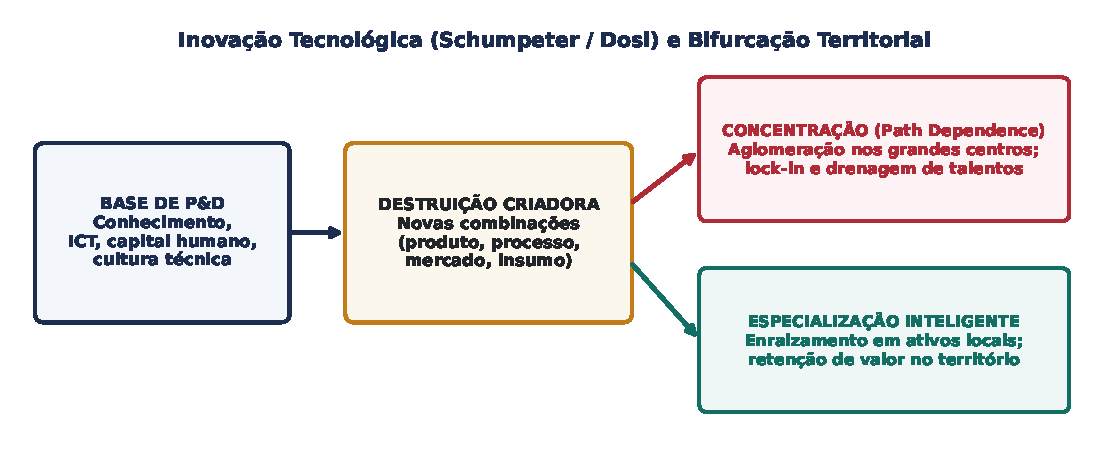
\includegraphics[width=0.94\textwidth]{figures/fig01_schumpeter_territorio.pdf}
  \caption{Integração entre dinâmica schumpeteriana (Mark I e Mark II), paradigmas e trajetórias tecnológicas (Kuhn e Dosi), intervenção pública (Mazzucato) e assimetrias do meio técnico-científico-informacional (Milton Santos).}
  \label{fig:schumpeter_territorio}
\end{figure}

\etapa{4}{Estudos de Caso e Aplicações Passo a Passo}

\begin{boxExemplo}{1}{Diagnóstico de EBT em Bioeconomia no Semiárido Baiano}
\passoEnunciado{Uma \textit{spin-off} acadêmica sediada em Feira de Santana (BA) desenvolve biofertilizantes encapsulados a partir de resíduos da mandiocultura. No último exercício fiscal, a empresa registrou receita operacional líquida de $\reais{1.200.000}$, despesas com P\&D de $\reais{270.000}$, ativos intangíveis avaliados em $\reais{960.000}$ (patente depositada no INPI e banco de cepas microbianas) e ativo imobilizado físico de $\reais{240.000}$.}
\passoDados{$R_{\text{op}} = \reais{1.200.000}$; $G_{\text{P\&D}} = \reais{270.000}$; $A_{\text{int}} = \reais{960.000}$; $A_{\text{imob}} = \reais{240.000}$.}
\passoPedido{Calcular a intensidade de P\&D ($I_{\text{P\&D}}$), a razão de intangibilidade ($\rho_{\text{int}}$) e classificar o empreendimento segundo a tipologia de EBTs.}
\passoMetodo{Aplicação das razões de intensidade tecnológica ($I_{\text{P\&D}} = G_{\text{P\&D}} / R_{\text{op}}$) e de estrutura patrimonial ($A_{\text{tot}} = A_{\text{int}} + A_{\text{imob}}$ e $\rho_{\text{int}} = A_{\text{int}} / A_{\text{tot}}$), seguida de enquadramento tipológico segundo Storey e Tether (1998) e Bailetti (2012).}
\passoContas{
  \begin{enumerate}[leftmargin=1.4em, itemsep=2pt]
    \item Cálculo do ativo total:
    \[
    A_{\text{tot}} = A_{\text{int}} + A_{\text{imob}} = 960.000 + 240.000 = \reais{1.200.000}
    \]
    \item Cálculo da intensidade de P\&D:
    \[
    I_{\text{P\&D}} = \frac{270.000}{1.200.000} \times 100\% = 0{,}225 \times 100\% = 22{,}5\%
    \]
    \item Cálculo da razão de intangibilidade:
    \[
    \rho_{\text{int}} = \frac{960.000}{1.200.000} \times 100\% = 0{,}80 \times 100\% = 80{,}0\%
    \]
  \end{enumerate}
}
\passoResposta{$I_{\text{P\&D}} = 22{,}5\%$ e $\rho_{\text{int}} = 80{,}0\%$. Trata-se de uma \textit{Spin-off} Acadêmica com perfil híbrido de \textit{Deep Tech} biotecnológica e Tecnologia Agroindustrial territorialmente enraizada.}
\passoVerificacao{Uma intensidade de P\&D de $22{,}5\%$ supera em mais de quatro vezes o limiar clássico de $5\%$ para setores de alta tecnologia, e $80\%$ do patrimônio está ancorado em conhecimento protegido. O resultado é consistente com uma EBT em estágio de validação de mercado e exige garantias financeiras baseadas em recebíveis ou subvenção, pois o baixo imobilizado limita o acesso a crédito bancário convencional.}
\end{boxExemplo}

\begin{boxExemplo}{2}{Transição Mark I para Mark II e Valor Presente do Ciclo de Maturação}
\passoEnunciado{Considere dois projetos de inovação em sensores ambientais: o Projeto A (regime \textit{Mark I}, startup independente) exige aporte único inicial de $\reais{300.000}$ em $t=0$ e gera um fluxo líquido único de $\reais{520.000}$ em $t=4$ anos após a certificação; o Projeto B (regime \textit{Mark II}, divisão de P\&D de empresa consolidada com rede comercial pronta) exige $\reais{300.000}$ em $t=0$ e gera fluxo líquido único de $\reais{460.000}$ em $t=2$ anos. A taxa mínima de atratividade (custo de oportunidade do capital) é de $12\%$ ao ano.}
\passoDados{$I_0 = \reais{300.000}$; $F_A = \reais{520.000}$ em $t_A = 4$; $F_B = \reais{460.000}$ em $t_B = 2$; $r = 0{,}12$ a.a.}
\passoPedido{Calcular o Valor Presente Líquido (VPL) de cada regime e analisar por que o ciclo longo penaliza o entrante \textit{Mark I}.}
\passoMetodo{Desconto intertemporal simples em período único: $\text{VPL} = \frac{F_t}{(1+r)^t} - I_0$.}
\passoContas{
  \begin{enumerate}[leftmargin=1.4em, itemsep=2pt]
    \item Fator de desconto para $t=4$ a $12\%$ a.a.:
    \[
    (1 + 0{,}12)^4 = 1{,}12^2 \times 1{,}12^2 = 1{,}2544 \times 1{,}2544 = 1{,}57351936
    \]
    \item VPL do Projeto A (\textit{Mark I}):
    \[
    \text{VPL}_A = \frac{520.000}{1{,}57351936} - 300.000 = 330.469{,}40 - 300.000 = \reais{30.469{,}40}
    \]
    \item Fator de desconto para $t=2$ a $12\%$ a.a.:
    \[
    (1 + 0{,}12)^2 = 1{,}2544
    \]
    \item VPL do Projeto B (\textit{Mark II}):
    \[
    \text{VPL}_B = \frac{460.000}{1{,}2544} - 300.000 = 366.709{,}18 - 300.000 = \reais{66.709{,}18}
    \]
  \end{enumerate}
}
\passoResposta{$\text{VPL}_A = \reais{30.469{,}40}$ e $\text{VPL}_B = \reais{66.709{,}18}$. Embora o retorno nominal de A seja maior ($\reais{520.000}$ contra $\reais{460.000}$), o projeto \textit{Mark II} apresenta VPL mais que dobrado devido à redução do ciclo de maturação pela metade.}
\passoVerificacao{O cálculo evidencia a vantagem estrutural das grandes empresas no regime \textit{Mark II}: ao disporem de canais de distribuição e escala prévia, encurtam o tempo até o mercado. Para que startups \textit{Mark I} sobrevivam com ciclos de $4$ a $8$ anos, tornam-se indispensáveis mecanismos de capital paciente, incubação e subvenção pública.}
\end{boxExemplo}

\begin{boxExemplo}{3}{Modelagem de \textit{Path Dependence} e Custo de Superação de \textit{Lock-in}}
\passoEnunciado{Uma cooperativa regional de beneficiamento de fibras naturais opera sob uma trajetória tecnológica antiga baseada em motores a diesel (Paradigma A), com custo operacional anual de $\reais{180.000}$/ano. Uma EBT local propõe um sistema híbrido solar-biomassa (Paradigma B) com custo operacional de $\reais{95.000}$/ano. Entretanto, a substituição exige investimento em novos equipamentos de $\reais{260.000}$ e retreinamento de operadores de $\reais{40.000}$ (custo total de transição $C_{\text{trans}} = \reais{300.000}$). O horizonte de planejamento da cooperativa é de apenas $3$ anos, sem financiamento subsidiado.}
\passoDados{$C_{\text{op},A} = \reais{180.000}$/ano; $C_{\text{op},B} = \reais{95.000}$/ano; $C_{\text{trans}} = \reais{300.000}$; horizonte $H = 3$ anos (sem desconto para análise de \textit{payback} simples).}
\passoPedido{Calcular a economia operacional anual, o tempo de retorno simples ($T_{\text{payback}}$) e verificar se há \textit{lock-in} no horizonte de decisão da cooperativa.}
\passoMetodo{Cálculo da economia anual $\Delta C_{\text{op}} = C_{\text{op},A} - C_{\text{op},B}$ e do tempo de retorno simples $T_{\text{payback}} = C_{\text{trans}} / \Delta C_{\text{op}}$, comparando com $H$.}
\passoContas{
  \begin{enumerate}[leftmargin=1.4em, itemsep=2pt]
    \item Economia operacional anual:
    \[
    \Delta C_{\text{op}} = 180.000 - 95.000 = \reais{85.000}\text{/ano}
    \]
    \item Economia acumulada no horizonte de $3$ anos:
    \[
    E_{3\text{ anos}} = 3 \times 85.000 = \reais{255.000}
    \]
    \item Saldo líquido em $3$ anos:
    \[
    S_3 = E_{3\text{ anos}} - C_{\text{trans}} = 255.000 - 300.000 = -\reais{45.000}
    \]
    \item Tempo de retorno simples necessário:
    \[
    T_{\text{payback}} = \frac{300.000}{85.000} \approx 3{,}53\text{ anos}
    \]
  \end{enumerate}
}
\passoResposta{A economia anual é de $\reais{85.000}$, exigindo $3{,}53$ anos para recuperar o custo de transição. Como o horizonte de decisão da cooperativa é de $3$ anos ($S_3 = -\reais{45.000}$), o território permanece aprisionado (\textit{lock-in}) no Paradigma A.}
\passoVerificacao{Mesmo sendo o Paradigma B tecnicamente superior e menos poluente, a combinação de custo de transição elevado com horizonte decisório curto bloqueia a mudança tecnológica. Políticas públicas de crédito verde ou compra pública garantida são instrumentos racionais para estender o horizonte para além de $3{,}53$ anos e romper o \textit{lock-in}.}
\end{boxExemplo}

\begin{boxExemplo}{4}{Assimetria do Meio Técnico-Científico-Informacional (Milton Santos)}
\passoEnunciado{Considere um estado hipotético dividido em duas macrorregiões: a Região Metropolitana (RM), com $3{,}6$ milhões de habitantes e $180$ depósitos anuais de patentes de invenção, e o Interior Semiárido (IS), com $4{,}4$ milhões de habitantes e $22$ depósitos anuais de patentes. Os gastos públicos estaduais em infraestrutura de P\&D totalizam $\reais{50.000.000}$/ano, sendo $\reais{42.500.000}$ alocados na RM e $\reais{7.500.000}$ no IS.}
\passoDados{População: $P_{\text{RM}} = 3{,}6\text{ mi}$, $P_{\text{IS}} = 4{,}4\text{ mi}$ ($P_{\text{tot}} = 8{,}0\text{ mi}$). Patentes: $N_{\text{RM}} = 180$, $N_{\text{IS}} = 22$ ($N_{\text{tot}} = 202$). Fomento: $F_{\text{RM}} = \reais{42{,}5\text{ mi}}$, $F_{\text{IS}} = \reais{7{,}5\text{ mi}}$ ($F_{\text{tot}} = \reais{50{,}0\text{ mi}}$).}
\passoPedido{Calcular a densidade de patentes por $100$ mil habitantes, o fomento \textit{per capita} em cada região e a razão de desigualdade entre RM e IS.}
\passoMetodo{Cálculo das taxas padronizadas por $100.000$ habitantes ($d_i = \frac{N_i}{P_i} \times 100.000$), fomento \textit{per capita} ($f_i = F_i / P_i$) e razão de disparidade ($R = d_{\text{RM}} / d_{\text{IS}}$).}
\passoContas{
  \begin{enumerate}[leftmargin=1.4em, itemsep=2pt]
    \item Densidade de patentes por $100$ mil habitantes:
    \[
    d_{\text{RM}} = \frac{180}{3.600.000} \times 100.000 = 5{,}00\text{ patentes / 100 mil hab.}
    \]
    \[
    d_{\text{IS}} = \frac{22}{4.400.000} \times 100.000 = 0{,}50\text{ patentes / 100 mil hab.}
    \]
    \item Razão de disparidade patentária:
    \[
    R_{\text{pat}} = \frac{5{,}00}{0{,}50} = 10{,}0\text{ vezes}
    \]
    \item Fomento \textit{per capita} em P\&D:
    \[
    f_{\text{RM}} = \frac{42.500.000}{3.600.000} = \reais{11{,}81}\text{/hab.} \qquad
    f_{\text{IS}} = \frac{7.500.000}{4.400.000} = \reais{1{,}70}\text{/hab.}
    \]
    \item Razão de disparidade de fomento:
    \[
    R_{\text{fom}} = \frac{11{,}81}{1{,}70} \approx 6{,}95\text{ vezes}
    \]
  \end{enumerate}
}
\passoResposta{A RM apresenta $5{,}00$ patentes/$100$ mil hab. e $\reais{11{,}81}$/hab. em fomento, contra $0{,}50$ patentes/$100$ mil hab. e $\reais{1{,}70}$/hab. no IS — uma assimetria de $10{,}0$ vezes na produção patentária e quase $7$ vezes no investimento \textit{per capita}.}
\passoVerificacao{Esses números materializam a seletividade espacial descrita por Milton Santos: embora o Interior concentre $55\%$ da população ($4{,}4$ de $8{,}0$ milhões), recebe apenas $15\%$ do fomento em P\&D ($\reais{7{,}5}$ de $\reais{50{,}0}$ milhões). Sem descentralização deliberada do meio técnico-científico-informacional, editais competitivos cegos ao território tendem a aprofundar essa concentração.}
\end{boxExemplo}

\begin{boxExemplo}{5}{Contraponto de Mazzucato: Subvenção Pública e Retenção Territorial ($\mu_{\text{loc}}$)}
\passoEnunciado{Uma EBT de tecnologia hídrica recebe uma subvenção econômica estadual não reembolsável de $G_{\text{pub}} = \reais{400.000}$ para desenvolver um dessalinizador solar modular. Esse aporte destrava $\reais{600.000}$ de investimento privado complementar ($G_{\text{tot}} = \reais{1.000.000}$). Nos dois anos seguintes, a operação da empresa gera no próprio território: $\reais{520.000}$ em salários de engenheiros e técnicos locais, $\reais{310.000}$ em compras de metalurgia local e $\reais{130.000}$ em tributos municipais e estaduais diretos. Os demais insumos são importados de fora da região.}
\passoDados{$G_{\text{pub}} = \reais{400.000}$; $G_{\text{priv}} = \reais{600.000}$; $G_{\text{tot}} = \reais{1.000.000}$; componentes locais: salários $\reais{520.000}$, fornecedores $\reais{310.000}$, tributos $\reais{130.000}$.}
\passoPedido{Calcular o fator de alavancagem privada ($A_{\text{priv}}$), o valor adicionado retido no território ($\Delta Y_{\text{loc}}$) e o multiplicador territorial sobre o recurso público ($\mu_{\text{loc,pub}}$) e sobre o P\&D total ($\mu_{\text{loc,tot}}$).}
\passoMetodo{Soma dos fluxos territorializados $\Delta Y_{\text{loc}} = W_{\text{loc}} + C_{\text{loc}} + T_{\text{loc}}$, cálculo da alavancagem $A_{\text{priv}} = G_{\text{priv}} / G_{\text{pub}}$ e dos multiplicadores $\mu_{\text{loc}}$.}
\passoContas{
  \begin{enumerate}[leftmargin=1.4em, itemsep=2pt]
    \item Fator de alavancagem privada:
    \[
    A_{\text{priv}} = \frac{600.000}{400.000} = 1{,}50\text{ (cada R\$ 1,00 público atraiu R\$ 1,50 privado)}
    \]
    \item Valor adicionado retido no território:
    \[
    \Delta Y_{\text{loc}} = 520.000 + 310.000 + 130.000 = \reais{960.000}
    \]
    \item Multiplicador territorial sobre o fomento público:
    \[
    \mu_{\text{loc,pub}} = \frac{960.000}{400.000} = 2{,}40
    \]
    \item Multiplicador territorial sobre o dispêndio total em P\&D:
    \[
    \mu_{\text{loc,tot}} = \frac{960.000}{1.000.000} = 0{,}96
    \]
  \end{enumerate}
}
\passoResposta{Alavancagem privada de $1{,}50\times$, retenção territorial de $\reais{960.000}$, multiplicador de $2{,}40$ sobre o aporte público e de $0{,}96$ sobre o gasto total.}
\passoVerificacao{Sob a ótica de Mazzucato, o Estado atuou como tomador de risco inicial viabilizando $\reais{600.000}$ privados e gerando $\reais{2{,}40}$ em circulação econômica local por real investido. Contudo, caso a empresa seja posteriormente adquirida e transfira sua sede e propriedade intelectual para outro polo, o multiplicador futuro cai e o território perde a renda tecnológica acumulada, justificando cláusulas contratuais de contrapartida territorial ou participação acionária pública.}
\end{boxExemplo}

\etapa{5}{Armadilhas Conceituais e Erros Mais Comuns}

\begin{boxErro}[Erro 1: Confundir Empresa Digital Genérica com \textit{Deep Tech}]
Muitos diagnósticos regionais classificam qualquer startup que utiliza um aplicativo ou plataforma de \textit{e-commerce} como empresa de alta intensidade tecnológica. Uma empresa de base digital que apenas adapta um modelo comercial existente sem P\&D proprietária possui baixa barreira técnica à imitação e $\rho_{\text{int}}$ reduzido quando excluído o gasto com marketing. Em políticas de fomento, equiparar revendas digitais a \textit{Deep Techs} distorce a alocação de subvenções de longo prazo.
\end{boxErro}

\begin{boxErro}[Erro 2: Reduzir Inovação à Invenção ou ao Depósito de Patentes]
Contabilizar apenas o número de patentes depositadas por universidades como medida de desenvolvimento territorial ignora a distinção schumpeteriana entre invenção e inovação. Patentes sem licenciamento, escalonamento industrial ou absorção produtiva local permanecem ativos ociosos no plano econômico, gerando custos de manutenção no INPI sem retorno territorial.
\end{boxErro}

\begin{boxErro}[Erro 3: Ignorar o Efeito do Ciclo de Maturação no Fluxo de Caixa]
Avaliar uma EBT de biotecnologia ou novos materiais com métricas de varejo de giro rápido conduz a decisões errôneas de investimento. Desconsiderar que o fator $(1+r)^{-t}$ comprime severamente o valor presente de receitas distantes leva empreendedores a subestimar a necessidade de capital paciente e a enfrentar insolvência técnica no chamado vale da morte.
\end{boxErro}

\begin{boxErro}[Erro 4: Tratar o Território como Espaço Neutro e Homogêneo]
Supor que boas ideias tecnológicas prosperam igualmente em qualquer município desconsidera as assimetrias do meio técnico-científico-informacional (Milton Santos). Em regiões periféricas, a ausência de laboratórios acreditados, consultoria de propriedade intelectual e compradores âncora eleva o custo de transação da EBT muito acima da média das metrópoles centrais.
\end{boxErro}

\etapa{6}{Lista de Exercícios (15 Questões Graduadas)}

\subsection*{Bloco A — Conceituais e Básicos (Questões 1 a 5)}

\begin{enumerate}[leftmargin=1.6em, itemsep=6pt]
  \item Explique, com base em Bailetti (2012) e Storey \& Tether (1998), por que a estrutura patrimonial de uma EBT difere radicalmente da estrutura de uma empresa comercial tradicional, destacando o papel dos ativos intangíveis e da propriedade intelectual.
  \espacoResolucao[1.8cm]

  \item Diferencie os quatro tipos de EBT apresentados no capítulo (\textit{Deep Tech}, Base Digital, \textit{Spin-off} Acadêmica e Tecnologia Social/Agro) quanto ao risco tecnológico predominante e ao ciclo de maturação.
  \espacoResolucao[1.8cm]

  \item Liste os cinco tipos de inovação propostos por Joseph Schumpeter (1911) e dê um exemplo territorialmente situado no Nordeste brasileiro para pelo menos dois deles.
  \espacoResolucao[1.8cm]

  \item Uma EBT de automação agrícola faturou $\reais{900.000}$ no ano e investiu $\reais{162.000}$ em P\&D. Calcule sua intensidade de P\&D ($I_{\text{P\&D}}$) e verifique se ela supera o patamar de referência de $5\%$ associado a setores de alta intensidade tecnológica.
  \espacoResolucao[1.8cm]

  \item Defina \textit{paradigma tecnológico} e \textit{trajetória tecnológica} segundo Giovanni Dosi (1982), explicando a relação desses conceitos com a noção de ciência normal em Thomas Kuhn (1962).
  \espacoResolucao[1.8cm]
\end{enumerate}

\subsection*{Bloco B — Intermediários e Aplicados (Questões 6 a 10)}

\begin{enumerate}[leftmargin=1.6em, itemsep=6pt, resume]
  \item Compare os regimes schumpeterianos \textit{Mark I} e \textit{Mark II} em relação à concentração de mercado, ao agente protagonista da inovação e à cumulatividade do conhecimento. Em qual regime se enquadra melhor uma \textit{spin-off} recém-criada em uma universidade estadual? Justifique.
  \espacoResolucao[2.0cm]

  \item Uma indústria de cerâmica vermelha no interior da Bahia gasta $\reais{240.000}$/ano com lenha nativa em fornos antigos. A adoção de fornos contínuos com biomassa residual certificada reduz o custo anual para $\reais{150.000}$/ano, mas exige investimento inicial de $\reais{315.000}$. Calcule o tempo de retorno simples ($T_{\text{payback}}$) e discuta como esse resultado ilustra o fenômeno de \textit{lock-in} quando os empresários operam com horizonte de $2{,}5$ anos.
  \espacoResolucao[2.2cm]

  \item Analise criticamente a tese de Mariana Mazzucato sobre o Estado Empreendedor frente ao conceito de destruição criadora de Schumpeter. Que mecanismos institucionais podem evitar a assimetria entre socialização dos riscos e privatização dos lucros?
  \espacoResolucao[2.0cm]

  \item Um projeto de EBT recebe $\reais{250.000}$ de subvenção pública e atrai $\reais{500.000}$ de investidores anjo. Nos três anos subsequentes, a empresa gera $\reais{450.000}$ em folha salarial local, $\reais{200.000}$ em compras regionais e $\reais{100.000}$ em tributos locais. Calcule o fator de alavancagem privada e o multiplicador territorial sobre o recurso público ($\mu_{\text{loc,pub}}$).
  \espacoResolucao[2.2cm]

  \item Com base em Milton Santos, explique como a desigualdade do meio técnico-científico-informacional entre metrópoles e regiões periféricas afeta a retenção de talentos e a apropriação de valor por EBTs nordestinas.
  \espacoResolucao[2.0cm]
\end{enumerate}

\subsection*{Bloco C — Questões Objetivas de Fixação (Questões 11 a 15)}

\begin{enumerate}[leftmargin=1.6em, itemsep=6pt, resume]
  \item Sobre as características estruturais das Empresas de Base Tecnológica (EBTs), assinale a alternativa \textbf{correta}:
  \begin{alternativas}
    \item O valor de uma EBT concentra-se prioritariamente em imóveis e estoques físicos, o que facilita o acesso imediato ao crédito bancário tradicional.
    \item Toda empresa que utiliza redes sociais para vendas configura uma \textit{Deep Tech} devido à adoção do meio digital.
    \item O ciclo longo de maturação e o predomínio de ativos intangíveis tornam a proteção por propriedade intelectual e o capital paciente elementos críticos para a sobrevivência da firma.
    \item A intensidade de P\&D de uma EBT madura deve ser inferior a $1\%$ da receita líquida para garantir lucratividade operacional.
    \item \textit{Spin-offs} acadêmicas não utilizam propriedade intelectual oriunda de universidades, pois dependem exclusivamente de aquisições de mercado.
  \end{alternativas}

  \item Na transição descrita por Schumpeter entre o modelo \textit{Mark I} (1911) e o modelo \textit{Mark II} (1942), observa-se que:
  \begin{alternativas}
    \item O modelo \textit{Mark II} substitui a P\&D interna rotinizada pelo improviso exclusivo de microempresários individuais sem capital.
    \item O modelo \textit{Mark I} caracteriza-se por alta concentração monopolista e barreiras intransponíveis à entrada de novas firmas.
    \item A destruição criadora elimina apenas empresas ineficientes sem afetar competências técnicas ou estruturas industriais estabelecidas.
    \item O regime \textit{Mark II} associa a inovação ao aprofundamento tecnológico e à cumulatividade em laboratórios de P\&D de grandes corporações.
    \item Nenhum dos dois regimes considera a introdução de novos métodos produtivos ou novas fontes de matéria-prima como formas de inovação.
  \end{alternativas}

  \item Em relação aos conceitos de paradigma tecnológico, trajetória tecnológica (Dosi, 1982) e aprisionamento (\textit{lock-in}), é correto afirmar que:
  \begin{alternativas}
    \item O \textit{lock-in} ocorre exclusivamente quando uma tecnologia é superior em eficiência energética a todas as suas concorrentes.
    \item A dependência de trajetória (\textit{path dependence}) implica que decisões históricas e retornos crescentes de adoção condicionam a evolução futura da tecnologia.
    \item Trajetórias tecnológicas evoluem de forma completamente independente de regras econômicas ou científicas acumuladas.
    \item O conceito de paradigma tecnológico nega qualquer analogia com a noção de paradigma científico formulada por Thomas Kuhn.
    \item Custos de transição nulos garantem a permanência indefinida de um sistema em estado de \textit{lock-in}.
  \end{alternativas}

  \item Uma empresa de tecnologia ambiental possui ativo intangível de $\reais{1.050.000}$ e ativo imobilizado de $\reais{450.000}$. A razão de intangibilidade ($\rho_{\text{int}}$) dessa empresa é igual a:
  \begin{alternativas}
    \item $30{,}0\%$
    \item $42{,}8\%$
    \item $57{,}1\%$
    \item $70{,}0\%$
    \item $85{,}0\%$
  \end{alternativas}

  \item Segundo a perspectiva crítica de Milton Santos sobre o meio técnico-científico-informacional, regiões periféricas enfrentam maior dificuldade para reter valor gerado por EBTs principalmente porque:
  \begin{alternativas}
    \item A internet elimina totalmente as diferenças geográficas de infraestrutura científica e financeira entre territórios.
    \item A distribuição seletiva de infraestrutura informacional, laboratórios, capital e serviços especializados concentra luminosidades em poucos polos centrais.
    \item Empresas de tecnologia não interagem com o espaço geográfico, operando em mercados puramente abstratos.
    \item O território periférico impede legalmente o depósito de patentes junto aos escritórios nacionais de propriedade intelectual.
    \item A presença de universidades locais elimina automaticamente qualquer assimetria espacial de renda e financiamento.
  \end{alternativas}
\end{enumerate}

\etapa{7}{Questões de Alta Complexidade (Estilo ANPAD / Pós-Graduação / CT\&I)}

\begin{enumerate}[leftmargin=1.6em, itemsep=8pt]
  \item \textbf{(Estilo Pós-Graduação / CT\&I)} Analise as proposições abaixo sobre a dinâmica tecnológica, o Estado Empreendedor e o desenvolvimento territorial:
  \begin{itemize}[leftmargin=1.2em, itemsep=2pt]
    \item[I.] Para Mazzucato, o financiamento público nas fases iniciais de alta incerteza tecnológica reduz o risco privado, mas sem mecanismos de contrapartida pode gerar assimetria entre socialização de riscos e privatização de ganhos.
    \item[II.] A ocorrência de \textit{path dependence} demonstra que mercados perfeitamente competitivos sempre selecionam instantaneamente a tecnologia de menor custo ambiental no longo prazo.
    \item[III.] No conceito de meio técnico-científico-informacional de Milton Santos, a densidade desigual de ciência, técnica e informação explica por que territórios periféricos frequentemente exportam cérebros e importam soluções tecnológicas acabadas.
  \end{itemize}
  Está correto o que se afirma em:
  \begin{alternativas}
    \item I, apenas.
    \item II, apenas.
    \item I e III, apenas.
    \item II e III, apenas.
    \item I, II e III.
  \end{alternativas}

  \item \textbf{(Estilo ANPAD / Gestão da Inovação)} Uma \textit{spin-off} de biotecnologia recebeu proposta de investimento para dois caminhos de desenvolvimento. No Caminho X, obtém retorno líquido único de $\reais{800.000}$ após $3$ anos com investimento inicial de $\reais{500.000}$. No Caminho Y, recebe uma subvenção não reembolsável que reduz seu desembolso inicial privado para $\reais{350.000}$, mantendo o retorno líquido de $\reais{800.000}$ em $3$ anos. Considerando custo de capital de $10\%$ ao ano ($(1{,}10)^3 = 1{,}331$), a variação absoluta no VPL privado da firma proporcionada pela subvenção é de:
  \begin{alternativas}
    \item $\reais{101.051{,}84}$
    \item $\reais{150.000{,}00}$
    \item $\reais{251.051{,}84}$
    \item $\reais{300.000{,}00}$
    \item $\reais{450.000{,}00}$
  \end{alternativas}

  \item \textbf{(Estilo Concurso CT\&I / FINEP)} Em uma avaliação de política pública de inovação regional, verificou-se que um programa estadual priorizou exclusivamente editais de subvenção baseados em mérito científico abstrato, sem critérios de enraizamento territorial. Como resultado, $82\%$ dos recursos foram captados por dois bairros da capital, enquanto municípios do interior com cadeias agroindustriais consolidadas captaram menos de $5\%$. À luz do referencial teórico deste capítulo, esse resultado evidencia:
  \begin{alternativas}
    \item O triunfo do modelo \textit{Mark I} sobre a concentração corporativa do modelo \textit{Mark II}.
    \item A superação definitiva do \textit{lock-in} institucional nas regiões interioranas.
    \item A reprodução das assimetrias do meio técnico-científico-informacional por políticas neutras ao espaço.
    \item A irrelevância das instituições públicas de ensino e pesquisa para a geração de \textit{spin-offs}.
    \item A comprovação de que tecnologias sociais possuem maior intensidade de patentes que \textit{Deep Techs}.
  \end{alternativas}
\end{enumerate}

\begin{boxDica}[Contraponto Crítico e Prática Territorial (Conexão AV1 e AV3)]
Na \textbf{AV1}, as questões exigem que você articule teoria econômica da inovação com leitura espacial: não basta citar Schumpeter ou Dosi isoladamente; é preciso demonstrar como o ciclo de maturação e o \textit{lock-in} afetam uma firma situada fora dos grandes centros. Já na \textbf{AV3} (projeto final territorializado), ao propor uma solução tecnológica para o território baiano ou nordestino, explicite qual é a trajetória tecnológica dominante que o projeto pretende tensionar, qual o ciclo estimado de maturação e como a empresa reterá valor adicionado localmente ($\mu_{\text{loc}}$).
\end{boxDica}

\clearpage
\etapa{8}{Gabarito Comentado (Questões 1 a 18)}

\begin{boxGabarito}[Respostas Comentadas — Exercícios 1 a 15 e Questões de Alta Complexidade 16 a 18]
\begin{enumerate}[leftmargin=1.6em, itemsep=4pt]
  \item \textbf{Resposta:} Diferentemente de firmas comerciais baseadas em estoque e giro rápido de mercadorias, a EBT ancora sua vantagem competitiva em conhecimento científico-tecnológico complexo (Storey \& Tether, 1998) e na mobilização de ativos especializados (Bailetti, 2012). Seu balanço patrimonial concentra-se em ativos intangíveis (patentes, software, \textit{know-how}), cuja apropriação econômica depende da proteção via propriedade intelectual para compensar o longo ciclo de P\&D.
  \item \textbf{Resposta:} \textit{Deep Techs} possuem alto risco científico-técnico e ciclo longo (3 a 10 anos); empresas de Base Digital têm risco predominantemente de mercado/adoção e ciclo mais curto; \textit{Spin-offs} Acadêmicas nascem da transferência de tecnologia universitária e enfrentam transição cultural da bancada ao mercado; Tecnologias Sociais/Agro combinam conhecimento técnico e saberes locais com foco em apropriação comunitária e cadeias territoriais.
  \item \textbf{Resposta:} Os 5 tipos de Schumpeter (1911) são: (1) novo bem ou qualidade; (2) novo método de produção; (3) abertura de novo mercado; (4) nova fonte de matéria-prima/insumos; (5) nova organização da indústria. Exemplos no Nordeste: bioinsumos adaptados ao Semiárido para substituir fertilizantes importados (tipo 4) ou consórcio digital de cooperativas de caprinocultura para venda direta (tipo 5).
  \item \textbf{Resposta:} $I_{\text{P\&D}} = (162.000 / 900.000) \times 100\% = 18{,}0\%$. Sim, supera amplamente o limiar de referência de $5\%$.
  \item \textbf{Resposta:} Para Dosi (1982), paradigma tecnológico é o modelo padrão de definição e solução de problemas técnicos (em analogia ao paradigma científico de Kuhn, 1962), enquanto trajetória tecnológica é o vetor de progresso incremental ao longo desse paradigma.
  \item \textbf{Resposta:} \textit{Mark I} caracteriza-se por baixa concentração, novos entrantes e liderança do empresário-inovador; \textit{Mark II} caracteriza-se por alta concentração, P\&D rotinizada em grandes corporações e alta cumulatividade. Uma \textit{spin-off} universitária recém-criada enquadra-se no regime \textit{Mark I}, pois atua como entrante disruptivo sem escala industrial prévia.
  \item \textbf{Resposta:} Economia anual $= 240.000 - 150.000 = \reais{90.000}$/ano. $T_{\text{payback}} = 315.000 / 90.000 = 3{,}5$ anos. Como o horizonte decisório é de $2{,}5$ anos (economia acumulada de $\reais{225.000} < \reais{315.000}$), o empresário rejeita a tecnologia mais limpa, evidenciando \textit{lock-in} econômico-financeiro.
  \item \textbf{Resposta:} Mazzucato mostra que o Estado assume o risco inicial das inovações radicais que alimentam a destruição criadora. Para evitar privatização assimétrica dos ganhos, recomendam-se cláusulas de retorno contingente (\textit{royalties}), participação acionária pública minoritária, metas de retenção de empregos locais e licenciamento aberto ou condicionado.
  \item \textbf{Resposta:} Alavancagem privada $= 500.000 / 250.000 = 2{,}00$. Retenção territorial $\Delta Y_{\text{loc}} = 450.000 + 200.000 + 100.000 = \reais{750.000}$. Multiplicador público $\mu_{\text{loc,pub}} = 750.000 / 250.000 = 3{,}00$.
  \item \textbf{Resposta:} A concentração de infraestrutura de pesquisa, conectividade, capital e serviços jurídicos nas metrópoles (luminosidades) faz com que EBTs periféricas enfrentem maiores custos de transação e sofram drenagem de talentos qualificados e de sede empresarial para polos centrais.
  \item \textbf{Gabarito: (C).} O ciclo longo e os intangíveis exigem PI e capital paciente.
  \item \textbf{Gabarito: (D).} O regime \textit{Mark II} (1942) descreve a rotinização da P\&D e o aprofundamento tecnológico em grandes corporações.
  \item \textbf{Gabarito: (B).} \textit{Path dependence} decorre de decisões históricas e retornos crescentes de adoção que condicionam a trajetória futura.
  \item \textbf{Gabarito: (D).} $A_{\text{tot}} = 1.050.000 + 450.000 = \reais{1.500.000}$. Logo, $\rho_{\text{int}} = (1.050.000 / 1.500.000) \times 100\% = 70{,}0\%$.
  \item \textbf{Gabarito: (B).} A seletividade espacial concentra infraestrutura científica e informacional em poucos nós luminosos.
  \item \textbf{Gabarito: (C).} A proposição II está incorreta porque \textit{path dependence} pode justamente aprisionar o mercado em tecnologias ambientalmente inferiores (\textit{lock-in}). I e III estão corretas.
  \item \textbf{Gabarito: (B).} $\text{VPL}_X = \frac{800.000}{1{,}331} - 500.000 = 601.051{,}84 - 500.000 = \reais{101.051{,}84}$. Com a subvenção, o investimento privado cai em $\reais{150.000}$ em $t=0$ ($\text{VPL}_Y = 601.051{,}84 - 350.000 = \reais{251.051{,}84}$). A variação absoluta é $251.051{,}84 - 101.051{,}84 = \reais{150.000{,}00}$.
  \item \textbf{Gabarito: (C).} Editais espacialmente cegos em territórios desiguais reproduzem a concentração do meio técnico-científico-informacional.
\end{enumerate}
\end{boxGabarito}

\begin{boxResumo}
\begin{itemize}[leftmargin=1.4em, itemsep=2pt]
  \item EBTs distinguem-se por alta intensidade de P\&D ($I_{\text{P\&D}}$), predomínio de intangíveis ($\rho_{\text{int}}$), proteção via PI e ciclo longo de maturação.
  \item Schumpeter opõe o empresário-inovador (\textit{Mark I}) à P\&D rotinizada (\textit{Mark II}), ambos inseridos na destruição criadora.
  \item Kuhn e Dosi explicam que a inovação segue paradigmas e trajetórias tecnológicas sujeitas a \textit{path dependence} e \textit{lock-in}.
  \item Mazzucato resgata o papel do Estado como tomador de risco inicial, enquanto Milton Santos revela as assimetrias espaciais do meio técnico-científico-informacional que desafiam o Nordeste e regiões periféricas.
\end{itemize}
\end{boxResumo}

\begin{boxTeste}
Responda sem consultar o texto e confira o gabarito logo abaixo:
\begin{enumerate}[leftmargin=1.4em, itemsep=3pt]
  \item (\V\ / \F) Uma empresa comercial que adquire softwares prontos de terceiros sem desenvolver P\&D ou ativos intangíveis proprietários configura uma \textit{Deep Tech}.
  \item (\V\ / \F) No modelo \textit{Mark II} de Schumpeter, a inovação é frequentemente internalizada em laboratórios de P\&D de grandes empresas com elevada cumulatividade.
  \item (\V\ / \F) O fenômeno de \textit{lock-in} ocorre quando custos de transição e retornos crescentes mantêm um setor preso a uma trajetória mesmo diante de alternativas mais eficientes.
  \item (\V\ / \F) Segundo Milton Santos, o meio técnico-científico-informacional distribui-se de maneira uniforme pelo território nacional, eliminando assimetrias regionais.
\end{enumerate}
\vspace{4pt}
\textbf{Gabarito do Checkpoint:} 1. \F\ (é usuária de tecnologia, não EBT produtora); 2. \V; 3. \V; 4. \F\ (sua distribuição é seletiva e assimétrica).
\end{boxTeste}

\chapter{Estruturas de Mercado, Barreiras de Entrada e Aglomerações Produtivas}
\tagAV{AV1 (30\%)}\ \tagTerritorio

\begin{capObjetivos}
Ao concluir este capítulo, você será capaz de:
\begin{itemize}[leftmargin=1.4em, itemsep=2pt]
  \item Distinguir as quatro estruturas clássicas de mercado (concorrência perfeita, monopólio, oligopólio e concorrência monopolística) quanto ao poder de precificação e à dinâmica de entrada.
  \item Aplicar o Modelo das Cinco Forças de Porter (1979; 1980) e as estratégias genéricas (liderança em custo, diferenciação e foco) à inserção competitiva de EBTs.
  \item Analisar barreiras econômicas, tecnológicas e regulatórias à entrada e à saída de mercados.
  \item Calcular e interpretar o Índice Herfindahl--Hirschman ($\text{HHI}$) e a variação de concentração ($\Delta \text{HHI}$) em operações de fusão ou entrada territorial.
  \item Explicar a transição da firma isolada para a Eficiência Coletiva em Arranjos Produtivos Locais (APLs), contrapondo a noção de espaço neutro ao território socialmente construído.
\end{itemize}
\end{capObjetivos}

\begin{capRevisao}
Para acompanhar a modelagem deste capítulo, relembre três fundamentos:
\begin{enumerate}[leftmargin=1.4em, itemsep=2pt]
  \item \textbf{Participação de mercado (\textit{market share}):} fração $s_i = q_i / Q_{\text{tot}}$ (em proporção de $0$ a $1$ ou em pontos percentuais de $0$ a $100$) detida pela firma $i$ nas vendas totais do setor relevante.
  \item \textbf{Economias de escala:} redução do custo médio unitário ($\text{CMe} = C_{\text{tot}} / Q$) à medida que o volume produzido $Q$ cresce, diluindo os custos fixos.
  \item \textbf{Custos afundados (\textit{sunk costs}):} investimentos específicos já realizados que não podem ser recuperados caso a empresa encerre suas atividades no setor.
\end{enumerate}
\end{capRevisao}

\etapa{3}{Estruturas de Mercado, Estratégia Competitiva e Eficiência Coletiva}

\begin{boxSimbolo}[Vocabulário Conceitual e Notação do Capítulo]
\begin{tabularx}{\linewidth}{@{}l X@{}}
  \toprule
  \textbf{Símbolo / Termo} & \textbf{Significado Analítico e Unidade} \\
  \midrule
  $s_i$ & Participação de mercado (\textit{market share}) da empresa $i$, expressa em \% ($0$ a $100$) ou proporção ($0$ a $1$). \\
  $\text{HHI}$ & Índice Herfindahl--Hirschman de concentração de mercado ($0$ a $10.000$ na escala percentual). \\
  $\Delta \text{HHI}$ & Variação do $\text{HHI}$ decorrente da fusão entre duas firmas $A$ e $B$ ($\Delta \text{HHI} = 2 s_A s_B$). \\
  $CR_k$ & Razão de concentração das $k$ maiores empresas do mercado ($CR_k = \sum_{i=1}^k s_i$). \\
  EME & Escala Mínima Eficiente: menor nível de produção em que o custo médio de longo prazo atinge seu mínimo. \\
  APL & Arranjo Produtivo Local: aglomeração territorial de agentes econômicos, políticos e sociais com foco em conjunto específico de atividades. \\
  EC & Eficiência Coletiva (Schmitz): vantagem competitiva derivada de economias externas locais somadas à ação conjunta deliberada. \\
  \bottomrule
\end{tabularx}
\end{boxSimbolo}

\section{Estruturas Clássicas de Mercado e Poder de Precificação}

A capacidade de uma Empresa de Base Tecnológica capturar valor depende diretamente da estrutura do mercado em que ingressa. Na teoria microeconômica, os mercados organizam-se em quatro arquétipos principais conforme o número de ofertantes, o grau de diferenciação do produto e a altura das barreiras à entrada. Na \textbf{Concorrência Perfeita}, um grande número de compradores e vendedores atomizados negocia produto homogêneo sob informação simétrica e livre entrada e saída, de modo que nenhuma firma controla o preço e todas atuam como tomadoras de preço ($P = \text{CMg}$ no equilíbrio de longo prazo). No extremo oposto encontra-se o \textbf{Monopólio}, caracterizado por um único ofertante de um bem ou serviço sem substitutos próximos, protegido por barreiras legais como patentes e concessões, pelo controle de insumo essencial ou por monopólio natural decorrente de custos fixos elevados frente à demanda, o que permite à firma definir preço ou quantidade e apropriar-se de rendas monopolistas.

Entre esses dois polos situam-se as estruturas mais frequentes na trajetória de EBTs. No \textbf{Oligopólio}, um pequeno número de grandes empresas domina a oferta e gera forte interdependência estratégica nas decisões de preço, capacidade e P\&D, compondo a estrutura típica de setores \textit{Mark II} como telecomunicações, semicondutores e defensivos agrícolas. Já na \textbf{Concorrência Monopolística}, numerosas firmas ofertam produtos diferenciados por marca, \textit{design}, funcionalidade ou atendimento localizado sob barreiras moderadas, conferindo a cada firma poder de mercado local sobre seu nicho, ainda que lucros extraordinários atraiam novos entrantes no longo prazo.

\section{Cinco Forças de Porter, Estratégias Genéricas e Barreiras}

Michael Porter (1979; 1980) estruturou a análise da atratividade setorial ao mostrar que a rentabilidade de uma indústria resulta da interação simultânea de cinco forças competitivas. Esse campo de forças combina a \textbf{rivalidade entre concorrentes existentes} e a \textbf{ameaça de novos entrantes} com a pressão exercida pela \textbf{ameaça de produtos ou serviços substitutos}, pelo \textbf{poder de barganha dos compradores} e pelo \textbf{poder de barganha dos fornecedores}.

Para posicionar-se de maneira defensável diante dessas forças, Porter (1980) propôs três \textbf{estratégias genéricas}. A \textbf{liderança em custo total} apoia-se em escala e eficiência operacional para ofertar preços menores, ao passo que a \textbf{diferenciação} constrói atributos únicos percebidos pelo cliente que justificam um prêmio de preço. A terceira via corresponde ao \textbf{foco}, voltado à atuação concentrada em um segmento, nicho tecnológico ou recorte territorial específico, operando tanto pela via do custo quanto pela diferenciação.

As \textbf{barreiras à entrada} determinam quão difícil é para uma nova EBT ingressar em um setor, envolvendo economias de escala exigidas na entrada, diferenciação e lealdade à marca, requisitos elevados de capital inicial, custos de mudança para o comprador, acesso restrito a canais de distribuição, desvantagens de custo independentes de escala (como patentes e curvas de aprendizagem) e regulação governamental (licenças sanitárias, ambientais ou registros no MAPA/ANVISA). De modo complementar, as \textbf{barreiras à saída} decorrem de ativos altamente especializados, custos fixos rescisórios, inter-relações estratégicas e compromissos sociais que mantêm empresas operando mesmo com margens negativas, acirrando a rivalidade do setor.

\begin{boxFormula}[Índice Herfindahl--Hirschman ($\text{HHI}$) de Concentração de Mercado]
\textbf{Origem.} Desenvolvido independentemente por Albert O. Hirschman (1945) e Orris C. Herfindahl (1950), é o indicador padrão utilizado por autoridades antitruste como o CADE (Brasil) e o DOJ/FTC (EUA) para medir concentração horizontal.

\textbf{Variáveis.} O cálculo considera o número total de empresas atuantes no mercado relevante $N$, a participação de mercado da empresa $i$ em pontos percentuais $s_i$ ($0 \le s_i \le 100$, com $\sum_{i=1}^N s_i = 100$) e as participações percentuais $s_A$ e $s_B$ de duas empresas candidatas a fusão ou aquisição.

\textbf{Fórmulas passo a passo:}
\[
\text{HHI} = \sum_{i=1}^{N} s_i^2
\qquad\qquad
\Delta \text{HHI} = \text{HHI}_{\text{pós}} - \text{HHI}_{\text{pré}} = (s_A + s_B)^2 - (s_A^2 + s_B^2) = 2 s_A s_B
\]

\textbf{Critérios interpretativos (escala $0$ a $10.000$).} Mercados com $\text{HHI} < 1.500$ são classificados como não concentrados, indicando estrutura competitiva. Quando $1.500 \le \text{HHI} \le 2.500$, observa-se concentração moderada, ao passo que valores de $\text{HHI} > 2.500$ caracterizam mercados altamente concentrados, correspondendo a oligopólio restrito ou a monopólio no limite de $\text{HHI} = 10.000$.

\textbf{Exemplo rápido.} Um mercado com $4$ empresas de participações $40\%$, $30\%$, $20\%$ e $10\%$ tem $\text{HHI} = 40^2 + 30^2 + 20^2 + 10^2 = 1.600 + 900 + 400 + 100 = 3.000$ (altamente concentrado). Se as duas menores ($20\%$ e $10\%$) se fundirem, $\Delta \text{HHI} = 2 \times 20 \times 10 = 400$, elevando o índice para $3.400$.
\end{boxFormula}

\section{Da Firma Isolada à Eficiência Coletiva em APLs e Território Social}

O modelo porteriano tradicional analisa a firma individual em confronto com forças externas. Contudo, pequenas e médias empresas tecnológicas enfrentam desvantagens severas de escala quando atuam isoladas. Hubert Schmitz (1995; 1999) evidenciou que a aglomeração geográfica em \textbf{Arranjos Produtivos Locais (APLs)} permite superar tais limitações por meio da \textbf{Eficiência Coletiva}, resultante da combinação de dois componentes complementares.

O primeiro componente abrange as \textbf{economias externas marshallianas} (não intencionais ou passivas), que reúnem benefícios gerados espontaneamente pela concentração espacial de firmas similares por meio da formação de um mercado de trabalho especializado, da atração de fornecedores dedicados de insumos, manutenção e serviços técnicos e dos transbordamentos tecnológicos e informacionais (\textit{spillovers}). O segundo componente corresponde à \textbf{ação conjunta deliberada} (intencional ou ativa), expressa na cooperação consciente entre empresas e instituições locais em arranjos horizontais (consórcios de compra, laboratórios compartilhados, certificação coletiva e feiras) ou verticais (programas de qualificação de fornecedores e codesenvolvimento tecnológico).

\begin{boxConceito}[Contraponto Crítico: Espaço Neutro vs. Território Socialmente Construído]
Na economia espacial neoclássica e em leituras simplificadas de clusters, o espaço é tratado como um \textbf{plano neutro e isotrópico}, no qual a localização ótima resulta apenas da minimização de custos de transporte e fatores. Em contraste, a geografia econômica crítica e a abordagem territorial latino-americana entendem o \textbf{território como construção social, histórica e política}. A simples aglomeração produtiva exige governança ativa para gerar eficiência coletiva, pois relações assimétricas de poder entre grandes compradores e microprodutores, desconfiança institucional, captura de consórcios por elites locais ou precarização do trabalho podem bloquear a cooperação e transformar um polo produtivo em enclave extrativo sem desenvolvimento endógeno.
\end{boxConceito}

Essa passagem da concorrência atomizada para a cooperação territorializada reorganiza o posicionamento estratégico das pequenas firmas frente aos grandes concorrentes. Conforme ilustra a Figura~\ref{fig:porter_eficiencia_coletiva}, a articulação entre economias externas marshallianas e ação conjunta deliberada desloca a firma isolada da vulnerabilidade estrutural das Cinco Forças de Porter para um patamar superior de competitividade sistêmica em Arranjos Produtivos Locais.

\begin{figure}[H]
  \centering
  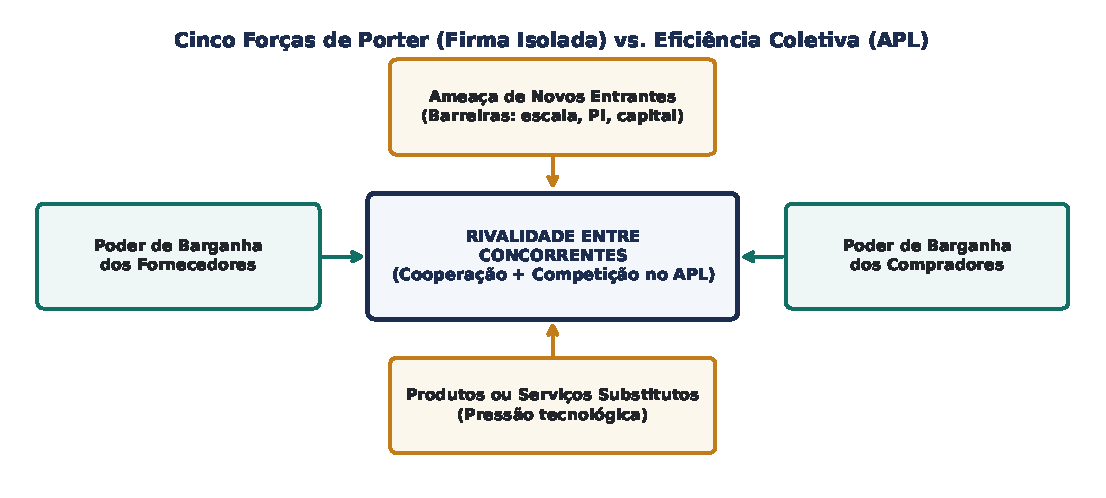
\includegraphics[width=0.94\textwidth]{figures/fig02_porter_eficiencia_coletiva.pdf}
  \caption{Transição analítica entre a firma isolada sob pressão das Cinco Forças de Porter e o ganho de Eficiência Coletiva (economias externas marshallianas + ação conjunta deliberada) em Arranjos Produtivos Locais.}
  \label{fig:porter_eficiencia_coletiva}
\end{figure}

\etapa{4}{Estudos de Caso e Aplicações Passo a Passo}

\begin{boxExemplo}{1}{Cálculo do Índice HHI, $CR_4$ e Impacto de Fusão em AgTechs}
\passoEnunciado{O mercado regional de softwares de gestão para agricultura familiar no Nordeste é atendido por cinco empresas com as seguintes participações nas vendas anuais: Empresa A ($35\%$), Empresa B ($25\%$), Empresa C ($20\%$), Empresa D ($12\%$) e Empresa E ($8\%$). A Empresa B propõe adquirir integralmente a Empresa D.}
\passoDados{$s_A = 35$; $s_B = 25$; $s_C = 20$; $s_D = 12$; $s_E = 8$ (soma $= 100\%$). Operação proposta: fusão B + D.}
\passoPedido{Calcular o $CR_4$ e o $\text{HHI}$ antes da fusão, a variação $\Delta \text{HHI}$ e o novo $\text{HHI}$ pós-fusão, classificando o grau de concentração segundo os critérios antitruste.}
\passoMetodo{Cálculo direto de $CR_4 = \sum_{i=1}^4 s_i$, $\text{HHI}_{\text{pré}} = \sum s_i^2$, $\Delta \text{HHI} = 2 s_B s_D$ e $\text{HHI}_{\text{pós}} = \text{HHI}_{\text{pré}} + \Delta \text{HHI}$.}
\passoContas{
  \begin{enumerate}[leftmargin=1.4em, itemsep=2pt]
    \item Razão de concentração das quatro maiores pré-fusão ($CR_4$):
    \[
    CR_4 = 35 + 25 + 20 + 12 = 92\%
    \]
    \item Cálculo do $\text{HHI}_{\text{pré}}$:
    \[
    \text{HHI}_{\text{pré}} = 35^2 + 25^2 + 20^2 + 12^2 + 8^2 = 1.225 + 625 + 400 + 144 + 64 = 2.458
    \]
    \item Variação $\Delta \text{HHI}$ com a fusão B + D ($s_{B+D} = 25 + 12 = 37\%$):
    \[
    \Delta \text{HHI} = 2 \times 25 \times 12 = 600
    \]
    \item Conferência direta do $\text{HHI}_{\text{pós}}$:
    \[
    \text{HHI}_{\text{pós}} = 35^2 + 37^2 + 20^2 + 8^2 = 1.225 + 1.369 + 400 + 64 = 3.058
    \]
    \[
    \text{Verificação:} \quad 2.458 + 600 = 3.058
    \]
  \end{enumerate}
}
\passoResposta{$CR_4 = 92\%$; $\text{HHI}_{\text{pré}} = 2.458$ (moderadamente concentrado); $\Delta \text{HHI} = 600$; $\text{HHI}_{\text{pós}} = 3.058$ (altamente concentrado).}
\passoVerificacao{Como o $\text{HHI}_{\text{pós}}$ ultrapassa $2.500$ com um salto $\Delta \text{HHI} = 600$ (muito acima do limiar típico de alerta de $200$ pontos), a operação gera risco anticompetitivo relevante, podendo elevar preços de licenciamento para cooperativas locais e criar barreiras à entrada de novas startups regionais.}
\end{boxExemplo}

\begin{boxExemplo}{2}{Matriz Ponderada das Cinco Forças de Porter para EBT Solar}
\passoEnunciado{Uma EBT de microinversores solares inteligentes avalia ingressar no segmento comercial de pequeno porte no Semiárido. Sua equipe atribuiu pesos estratégicos às Cinco Forças de Porter (soma $= 1{,}00$) e notas de pressão competitiva de $1$ (pressão muito baixa/favorável) a $5$ (pressão muito alta/desfavorável): Rivalidade ($w_1 = 0{,}30$, nota $4{,}0$); Novos Entrantes ($w_2 = 0{,}20$, nota $3{,}0$); Substitutos ($w_3 = 0{,}15$, nota $2{,}0$); Poder dos Compradores ($w_4 = 0{,}20$, nota $3{,}5$); Poder dos Fornecedores de chips asiáticos ($w_5 = 0{,}15$, nota $4{,}5$).}
\passoDados{Pesos $w = (0{,}30; 0{,}20; 0{,}15; 0{,}20; 0{,}15)$ e notas $N = (4{,}0; 3{,}0; 2{,}0; 3{,}5; 4{,}5)$.}
\passoPedido{Calcular o Índice Global de Pressão Setorial ($P_{\text{Porter}}$) e indicar qual estratégia genérica de Porter é mais defensável.}
\passoMetodo{Média aritmética ponderada $P_{\text{Porter}} = \sum_{j=1}^5 w_j N_j$.}
\passoContas{
  \begin{enumerate}[leftmargin=1.4em, itemsep=2pt]
    \item Contribuição ponderada de cada força:
    \[
    w_1 N_1 = 0{,}30 \times 4{,}0 = 1{,}20
    \]
    \[
    w_2 N_2 = 0{,}20 \times 3{,}0 = 0{,}60
    \]
    \[
    w_3 N_3 = 0{,}15 \times 2{,}0 = 0{,}30
    \]
    \[
    w_4 N_4 = 0{,}20 \times 3{,}5 = 0{,}70
    \]
    \[
    w_5 N_5 = 0{,}15 \times 4{,}5 = 0{,}675
    \]
    \item Soma ponderada total:
    \[
    P_{\text{Porter}} = 1{,}20 + 0{,}60 + 0{,}30 + 0{,}70 + 0{,}675 = 3{,}475\text{ (em escala de 1 a 5)}
    \]
  \end{enumerate}
}
\passoResposta{$P_{\text{Porter}} = 3{,}475$ (pressão competitivo-estrutural moderada a alta). A estratégia mais indicada é o \textbf{Foco com Diferenciação} em monitoramento térmico e assistência técnica local.}
\passoVerificacao{Competir por liderança em custo contra grandes fabricantes asiáticos (nota $4{,}5$ nos fornecedores e $4{,}0$ na rivalidade) inviabilizaria a EBT regional. O foco diferenciado (equipamento adaptado a altas temperaturas e suporte local ágil) reduz a sensibilidade a preço dos compradores e cria custos de mudança.}
\end{boxExemplo}

\begin{boxExemplo}{3}{Barreiras à Entrada e Escala Mínima Eficiente (EME) no Território}
\passoEnunciado{Para operar uma planta de envase asséptico de polpas funcionais da caatinga (como umbu e maracujá-do-mato) com certificação de exportação, a tecnologia impõe custos fixos anuais de $\text{CF} = \reais{900.000}$/ano e custo variável unitário de $\text{CVu} = \reais{4{,}00}$/litro. A demanda regional total do mercado endereçável é de $Q_{\text{merc}} = 600.000$ litros/ano, e o preço médio praticado no mercado é de $P = \reais{10{,}00}$/litro. Uma planta é considerada competitiva quando atinge a Escala Mínima Eficiente (EME) onde o custo médio unitário não ultrapassa $\reais{7{,}00}$/litro.}
\passoDados{$\text{CF} = \reais{900.000}$/ano; $\text{CVu} = \reais{4{,}00}$/L; $\text{CM}_{\text{alvo}} = \reais{7{,}00}$/L; $Q_{\text{merc}} = 600.000$ L/ano.}
\passoPedido{Calcular o volume correspondente à EME, o percentual do mercado regional que uma única planta precisa capturar para atingir a EME e o número máximo teórico de plantas eficientes comportadas pelo mercado.}
\passoMetodo{Custo médio $\text{CM}(Q) = \frac{\text{CF}}{Q} + \text{CVu}$. Igualar $\text{CM}(Q) = \text{CM}_{\text{alvo}}$ para encontrar $Q_{\text{EME}}$ e calcular a fração $s_{\text{EME}} = Q_{\text{EME}} / Q_{\text{merc}}$.}
\passoContas{
  \begin{enumerate}[leftmargin=1.4em, itemsep=2pt]
    \item Equação da Escala Mínima Eficiente:
    \[
    \frac{900.000}{Q_{\text{EME}}} + 4{,}00 = 7{,}00 \implies \frac{900.000}{Q_{\text{EME}}} = 3{,}00
    \]
    \[
    Q_{\text{EME}} = \frac{900.000}{3{,}00} = 300.000\text{ litros/ano}
    \]
    \item Participação de mercado exigida pela EME:
    \[
    s_{\text{EME}} = \frac{300.000}{600.000} \times 100\% = 50{,}0\%
    \]
    \item Número máximo de plantas na EME:
    \[
    N_{\max} = \frac{Q_{\text{merc}}}{Q_{\text{EME}}} = \frac{600.000}{300.000} = 2\text{ plantas}
    \]
  \end{enumerate}
}
\passoResposta{$Q_{\text{EME}} = 300.000$ L/ano; cada entrante precisa capturar $50\%$ do mercado regional; o território comporta no máximo $2$ plantas nessa escala.}
\passoVerificacao{O resultado demonstra como economias de escala formam uma barreira natural à entrada que induz estrutura oligopolista ($2$ firmas, $\text{HHI}$ mínimo de $50^2 + 50^2 = 5.000$). Uma alternativa territorial inteligente é a formação de uma agroindústria cooperativa compartilhada (ação conjunta) para diluir os $\reais{900.000}$ fixos entre dezenas de produtores.}
\end{boxExemplo}

\begin{boxExemplo}{4}{Quantificação da Eficiência Coletiva em Arranjo Produtivo Local}
\passoEnunciado{Considere uma microempresa isolada de confecção técnica/têxtil que produz $10.000$ peças/ano a um custo unitário base de $\reais{50{,}00}$/peça (total de $\reais{500.000}$/ano). Ao integrar-se a um APL estruturado no interior do estado, a empresa obtém dois ganhos distintos: (1) por economias externas marshallianas (proximidade de oficinas de manutenção e mão de obra treinada), reduz perdas e tempo ocioso em $8\%$ sobre o custo base; (2) por ação conjunta deliberada (consórcio de compras de tecido tecnológico e laboratório compartilhado de controle de qualidade), reduz em mais $12\%$ o custo já ajustado pelas economias externas. O consórcio cobra uma anuidade associativa fixa de $\reais{12.000}$/ano.}
\passoDados{$Q = 10.000$ peças; $\text{CM}_0 = \reais{50{,}00}$/peça; redução passiva $d_1 = 8\%$; redução ativa $d_2 = 12\%$; taxa associativa $F_{\text{assoc}} = \reais{12.000}$/ano.}
\passoPedido{Calcular o custo unitário após economias externas, o custo após ação conjunta (antes e depois da anuidade) e o ganho líquido anual em Eficiência Coletiva.}
\passoMetodo{Aplicação sequencial dos fatores $(1 - d_1)$ e $(1 - d_2)$, seguida da adição do custo fixo associativo diluído ($F_{\text{assoc}} / Q$).}
\passoContas{
  \begin{enumerate}[leftmargin=1.4em, itemsep=2pt]
    \item Custo unitário após economias externas marshallianas:
    \[
    \text{CM}_1 = 50{,}00 \times (1 - 0{,}08) = 50{,}00 \times 0{,}92 = \reais{46{,}00}\text{/peça}
    \]
    \item Custo unitário após ação conjunta deliberada (antes da anuidade):
    \[
    \text{CM}_2 = 46{,}00 \times (1 - 0{,}12) = 46{,}00 \times 0{,}88 = \reais{40{,}48}\text{/peça}
    \]
    \item Custo total anual no APL incluindo anuidade de $\reais{12.000}$:
    \[
    C_{\text{tot,APL}} = (10.000 \times 40{,}48) + 12.000 = 404.800 + 12.000 = \reais{416.800}\text{/ano}
    \]
    \item Custo unitário final líquido e economia total anual:
    \[
    \text{CM}_{\text{final}} = \frac{416.800}{10.000} = \reais{41{,}68}\text{/peça}
    \]
    \[
    \text{Ganho líquido anual} = 500.000 - 416.800 = \reais{83.200}\text{/ano} \quad (\text{redução líquida de } 16{,}64\%)
    \]
  \end{enumerate}
}
\passoResposta{$\text{CM}_1 = \reais{46{,}00}$, $\text{CM}_2 = \reais{40{,}48}$, $\text{CM}_{\text{final}} = \reais{41{,}68}$/peça e ganho líquido de $\reais{83.200}$/ano ($16{,}64\%$).}
\passoVerificacao{O exercício ilustra o núcleo da teoria de Schmitz: estar apenas geograficamente próximo gera $\reais{40.000}$ de economia passiva ($8\%$), mas a governança da ação conjunta acrescenta mais $\reais{43.200}$ líquidos após pagar a anuidade. O território socialmente organizado produz competitividade inacessível à firma isolada.}
\end{boxExemplo}

\begin{boxExemplo}{5}{Barreiras à Saída e Custos Afundados (\textit{Sunk Costs})}
\passoEnunciado{Uma empresa tradicional de processamento mineral investiu $\reais{2.000.000}$ em um forno rotativo dedicado cuja venda como sucata renderia apenas $\reais{250.000}$, além de enfrentar multa ambiental e rescisões trabalhistas de $\reais{350.000}$ caso encerre a operação hoje. No próximo ano, projeta-se receita de $\reais{1.100.000}$ e custos operacionais correntes de $\reais{1.220.000}$ (prejuízo operacional de $\reais{120.000}$).}
\passoDados{Investimento histórico $= \reais{2.000.000}$; valor de revenda $V_{\text{rev}} = \reais{250.000}$; custo de encerramento $C_{\text{enc}} = \reais{350.000}$; resultado operacional anual projetado $= -\reais{120.000}$.}
\passoPedido{Calcular o custo afundado (\textit{sunk cost}), o saldo líquido de saída imediata e explicar por que a firma pode optar por permanecer operando no curto prazo, agravando a rivalidade setorial.}
\passoMetodo{Cálculo do custo irrecuperável ($\text{SC} = I_0 - V_{\text{rev}}$) e comparação entre o fluxo de saída imediata ($V_{\text{rev}} - C_{\text{enc}}$) e a perda operacional de permanecer ($-\reais{120.000}$).}
\passoContas{
  \begin{enumerate}[leftmargin=1.4em, itemsep=2pt]
    \item Custo afundado do ativo dedicado:
    \[
    \text{SC} = 2.000.000 - 250.000 = \reais{1.750.000}
    \]
    \item Fluxo líquido de caixa caso decida sair hoje:
    \[
    F_{\text{saída}} = V_{\text{rev}} - C_{\text{enc}} = 250.000 - 350.000 = -\reais{100.000}
    \]
    \item Comparação com a manutenção da operação por mais $1$ ano (aguardando recuperação de preços): se permanecer, perde $\reais{120.000}$ no ano, mas preserva a opção de recuperar demanda; se sair, desembolsa $\reais{100.000}$ líquidos imediatamente e perde definitivamente o ativo produtivo.
  \end{enumerate}
}
\passoResposta{Custo afundado de $\reais{1.750.000}$ e saldo de saída imediata de $-\reais{100.000}$.}
\passoVerificacao{Em mercados com altas barreiras à saída (ativos específicos e altos encargos de encerramento), firmas deficitárias permanecem produzindo para cobrir parte dos custos ou aguardar reversão de ciclo, mantendo excesso de capacidade e intensificando a guerra de preços prevista por Porter.}
\end{boxExemplo}

\etapa{5}{Armadilhas Conceituais e Erros Mais Comuns}

\begin{boxErro}[Erro 1: Confundir Concentração de Mercado ($\text{HHI}$) com Lucro Garantido]
Um $\text{HHI}$ superior a $2.500$ indica alta concentração entre ofertantes atuais, mas não garante rentabilidade automática se a ameaça de substitutos ou o poder de barganha dos compradores (Forças 3 e 4 de Porter) forem extremos. Um monopólio local de transporte fluvial pode ter $\text{HHI} = 10.000$ e margens comprimidas pela concorrência do transporte rodoviário substituto.
\end{boxErro}

\begin{boxErro}[Erro 2: Misturar Escalas no Cálculo do Índice HHI]
Calcular o $\text{HHI}$ somando participações em proporção ($0{,}40^2 + 0{,}60^2 = 0{,}52$) e compará-lo diretamente com a faixa regulatória de $1.500$ a $2.500$ (que usa escala percentual de $0$ a $100$) é um erro clássico. Na escala percentual, $\text{HHI} \in (0, 10.000]$; na escala decimal, $\text{HHI}_{\text{dec}} \in (0, 1]$, sendo a conversão $\text{HHI} = 10.000 \times \text{HHI}_{\text{dec}}$.
\end{boxErro}

\begin{boxErro}[Erro 3: Reduzir APL a Simples Aglomeração Geográfica]
Muitos projetos territoriais chamam qualquer conjunto de empresas próximas de APL com eficiência coletiva. Sem ação conjunta deliberada (governança compartilhada, compras coletivas, inovação cooperativa), a simples proximidade espacial gera no máximo economias marshallianas passivas e pode degenerar em guerra predatória de preços entre vizinhos.
\end{boxErro}

\begin{boxErro}[Erro 4: Tentar Competir por Liderança em Custo em Nichos de Baixa Escala]
Startups e EBTs iniciantes frequentemente tentam vencer incumbentes baixando preços antes de atingir a Escala Mínima Eficiente (EME). Sem volume para diluir custos fixos de P\&D e estrutura, a estratégia de liderança em custo destrói o caixa inicial; o caminho viável na entrada costuma ser diferenciação ou foco territorial/tecnológico.
\end{boxErro}

\etapa{6}{Lista de Exercícios (15 Questões Graduadas)}

\subsection*{Bloco A: Conceituais e Básicos (Questões 1 a 5)}

\begin{enumerate}[leftmargin=1.6em, itemsep=6pt]
  \item Compare concorrência perfeita, concorrência monopolística e oligopólio quanto à diferenciação do produto, ao número de firmas e à capacidade de influenciar o preço de mercado.
  \espacoResolucao[1.8cm]

  \item Liste as Cinco Forças Competitivas de Porter (1979) e explique por que um alto poder de barganha de fornecedores especializados reduz a rentabilidade potencial de uma EBT.
  \espacoResolucao[1.8cm]

  \item Um mercado de serviços de geoprocessamento com drones é dividido igualmente entre $5$ empresas ($20\%$ cada). Calcule o $\text{HHI}$ desse mercado e classifique-o segundo as faixas usuais ($<1.500$, $1.500$--$2.500$, $>2.500$).
  \espacoResolucao[1.8cm]

  \item Diferencie barreiras à entrada de barreiras à saída, citando dois exemplos concretos de cada uma no contexto de empreendimentos industriais ou agroindustriais.
  \espacoResolucao[1.8cm]

  \item Defina \textit{Eficiência Coletiva} segundo Hubert Schmitz, explicando a diferença entre economias externas marshallianas e ação conjunta deliberada.
  \espacoResolucao[1.8cm]
\end{enumerate}

\subsection*{Bloco B: Intermediários e Aplicados (Questões 6 a 10)}

\begin{enumerate}[leftmargin=1.6em, itemsep=6pt, resume]
  \item Em um mercado regional de sensores de umidade do solo, quatro empresas detêm as seguintes participações: Firmas 1 ($40\%$), 2 ($30\%$), 3 ($15\%$) e 4 ($15\%$). Calcule o $\text{HHI}$ inicial, a variação $\Delta \text{HHI}$ caso as Firmas 3 e 4 se fundam, e o $\text{HHI}$ final após a fusão.
  \espacoResolucao[2.2cm]

  \item Uma pequena agroindústria de derivados de licuri possui custo fixo anual de $\reais{180.000}$ e custo variável unitário de $\reais{6{,}00}$/kg. Para atingir a Escala Mínima Eficiente (EME), seu custo médio unitário não pode ultrapassar $\reais{10{,}00}$/kg. Calcule a quantidade anual mínima ($Q_{\text{EME}}$) necessária para atingir essa eficiência.
  \espacoResolucao[2.2cm]

  \item Explique como uma EBT do Semiárido pode utilizar a estratégia genérica de \textbf{Foco com Diferenciação} para se proteger da rivalidade de grandes fabricantes multinacionais.
  \espacoResolucao[2.0cm]

  \item Em um APL de apicultura no Nordeste, $20$ associações produzem juntas $100.000$ kg de mel/ano a um custo médio de $\reais{14{,}00}$/kg. Por meio de economias externas locais, o custo cai $5\%$, e por meio de uma casa do mel e envase compartilhados (ação conjunta), cai mais $10\%$ sobre o valor já reduzido, mediante uma taxa anual compartilhada de $\reais{42.000}$ dividida pelo volume total. Calcule o custo unitário final por kg.
  \espacoResolucao[2.2cm]

  \item Discuta o contraponto entre ``espaço neutro'' e ``território socialmente construído'' aplicado à governança de um APL: por que a existência de muitas empresas próximas nem sempre gera inovação cooperativa?
  \espacoResolucao[2.0cm]
\end{enumerate}

\subsection*{Bloco C: Questões Objetivas de Fixação (Questões 11 a 15)}

\begin{enumerate}[leftmargin=1.6em, itemsep=6pt, resume]
  \item No Modelo das Cinco Forças de Porter, a presença de custos de mudança elevados para os clientes que desejam trocar de fornecedor de software atua diretamente para:
  \begin{alternativas}
    \item Reduzir o poder de barganha dos compradores e elevar a barreira à entrada de novos concorrentes.
    \item Eliminar completamente a necessidade de proteção por propriedade intelectual.
    \item Transformar o mercado em uma estrutura de concorrência perfeita com produto homogêneo.
    \item Aumentar o poder de barganha dos fornecedores de matérias-primas básicas.
    \item Reduzir as barreiras à saída das empresas incumbentes.
  \end{alternativas}

  \item Um setor apresenta quatro empresas com participações de $50\%$, $20\%$, $20\%$ e $10\%$. O Índice Herfindahl--Hirschman ($\text{HHI}$) desse mercado é:
  \begin{alternativas}
    \item $1.000$
    \item $2.400$
    \item $3.000$
    \item $3.400$
    \item $4.000$
  \end{alternativas}

  \item Na abordagem de Eficiência Coletiva (Schmitz), constituem exemplos de \textbf{economias externas marshallianas} (passivas) e de \textbf{ação conjunta deliberada} (ativa), respectivamente:
  \begin{alternativas}
    \item Consórcio de exportação e disponibilidade espontânea de mão de obra treinada na região.
    \item Disponibilidade espontânea de fornecedores locais de peças e criação de um laboratório de testes compartilhado pelas empresas.
    \item Guerra de preços entre firmas vizinhas e abertura de filiais em outro continente.
    \item Subsídio federal direto e monopólio legal por patente farmacêutica.
    \item Redução de impostos estaduais e venda isolada de commodities sem certificação.
  \end{alternativas}

  \item Sobre as estratégias genéricas de Porter (1980), assinale a alternativa \textbf{correta}:
  \begin{alternativas}
    \item A liderança em custo exige que a empresa opere sempre com baixos volumes e alta customização artesanal.
    \item A diferenciação busca entregar atributos únicos valorizados pelo comprador que permitam sustentar margem superior à média do setor.
    \item A estratégia de foco consiste em atender simultaneamente todos os segmentos de mercado com o menor preço possível.
    \item O modelo de Porter proíbe que empresas de base tecnológica atuem em nichos regionais.
    \item Barreiras à entrada altas e barreiras à saída baixas representam o pior cenário possível de rentabilidade setorial.
  \end{alternativas}

  \item Na análise de estruturas de mercado, um cenário caracterizado por \textbf{barreiras à entrada baixas} e \textbf{barreiras à saída altas} tende a gerar:
  \begin{alternativas}
    \item Retornos estáveis e elevados no longo prazo, com baixa rivalidade.
    \item Monopólio natural estável com regulação tarifária mínima.
    \item Retornos baixos e voláteis, pois novos concorrentes entram facilmente nos ciclos de alta e permanecem presos em guerras de preços nos ciclos de baixa.
    \item Eliminação imediata de todas as firmas ineficientes sem custos afundados.
    \item Transição automática para a concorrência perfeita sem diferenciação.
  \end{alternativas}
\end{enumerate}

\etapa{7}{Questões de Alta Complexidade (Estilo ANPAD / Pós-Graduação / CT\&I)}

\begin{enumerate}[leftmargin=1.6em, itemsep=8pt]
  \item \textbf{(Estilo ANPAD / Estratégia)} Em um mercado relevante de bioinsumos agrícolas composto por cinco firmas com participações $40\%$, $25\%$, $15\%$, $10\%$ e $10\%$, uma autoridade antitruste analisa duas propostas distintas de fusão: Proposta 1 (união das firmas de $40\%$ e $10\%$) e Proposta 2 (união das firmas de $25\%$ e $15\%$). Considerando a variação $\Delta \text{HHI}$, é correto afirmar que:
  \begin{alternativas}
    \item A Proposta 1 gera $\Delta \text{HHI} = 400$ e a Proposta 2 gera $\Delta \text{HHI} = 375$, portanto a Proposta 2 eleva mais a concentração.
    \item Ambas as propostas resultam no mesmo $\Delta \text{HHI} = 800$, pois envolvem o mesmo número de firmas remanescentes.
    \item A Proposta 1 gera $\Delta \text{HHI} = 800$ e a Proposta 2 gera $\Delta \text{HHI} = 750$, levando o mercado de um $\text{HHI}$ inicial de $2.650$ para $3.450$ ou $3.400$, respectivamente.
    \item O $\text{HHI}$ inicial do mercado é $1.850$ (moderadamente concentrado), tornando ambas as fusões isentas de análise.
    \item A Proposta 2 reduz o $\text{HHI}$ total por equilibrar as participações das duas maiores líderes.
  \end{alternativas}

  \item \textbf{(Estilo Pós-Graduação / Economia Regional)} Sobre a relação entre economias de aglomeração, Eficiência Coletiva e território socialmente construído, analise as assertivas:
  \begin{itemize}[leftmargin=1.2em, itemsep=2pt]
    \item[I.] Economias externas marshallianas explicam ganhos de produtividade decorrentes da proximidade espacial, mas não bastam para explicar respostas coordenadas a choques competitivos externos, que exigem ação conjunta deliberada.
    \item[II.] A concepção de território como espaço neutro garante que toda aglomeração industrial gere distribuição equitativa de renda e cooperação horizontal entre pequenas e grandes firmas.
    \item[III.] Em APLs periféricos, relações assimétricas de governança podem fazer com que grandes compradores externos capturem a maior parte dos ganhos da eficiência coletiva local.
  \end{itemize}
  Está correto o que se afirma em:
  \begin{alternativas}
    \item I, apenas.
    \item II, apenas.
    \item I e III, apenas.
    \item II e III, apenas.
    \item I, II e III.
  \end{alternativas}

  \item \textbf{(Estilo Concurso CT\&I / Desenvolvimento Regional)} Uma EBT de embalagens biodegradáveis de fécula de mandioca enfrenta forte poder de compra de grandes redes varejistas (Força 4 de Porter) e concorrência de embalagens plásticas convencionais (Força 3 de Porter). Para elevar sua defensabilidade estrutural sem entrar em guerra de preços, a decisão mais consistente com o referencial deste capítulo é:
  \begin{alternativas}
    \item Reduzir seus investimentos em P\&D e copiar exatamente o preço do plástico convencional, mesmo abaixo do custo médio.
    \item Buscar diferenciação certificada (compostabilidade e origem territorial) combinada com ação conjunta em consórcio de fornecedores locais para reduzir custos unitários de matéria-prima.
    \item Aumentar deliberadamente suas barreiras à saída imobilizando capital em máquinas sem uso alternativo.
    \item Operar em concorrência perfeita eliminando qualquer registro de patente ou marca própria.
    \item Transferir toda a cadeia produtiva para longe das áreas produtoras de mandioca, tratando a localização como espaço neutro.
  \end{alternativas}
\end{enumerate}

\begin{boxDica}[Contraponto Crítico e Prática Territorial (Conexão AV1 e AV3)]
Na \textbf{AV1}, lembre-se de que o $\text{HHI}$ mede concentração de oferta, enquanto as Cinco Forças de Porter avaliam a pressão estrutural completa do setor. Na \textbf{AV3}, ao desenhar o posicionamento competitivo do seu projeto territorial, evite propor que uma nova EBT vença grandes incumbentes apenas por preço baixo: mostre onde está a barreira de diferenciação, qual é a Escala Mínima Eficiente e como a articulação com um APL local (Eficiência Coletiva) viabiliza custos competitivos.
\end{boxDica}

\clearpage
\etapa{8}{Gabarito Comentado (Questões 1 a 18)}

\begin{boxGabarito}[Respostas Comentadas: Exercícios 1 a 15 e Questões de Alta Complexidade 16 a 18]
\begin{enumerate}[leftmargin=1.6em, itemsep=4pt]
  \item \textbf{Resposta:} Na concorrência perfeita há muitos ofertantes, produto homogêneo e nenhum poder de preço; na concorrência monopolística há muitos ofertantes com produtos diferenciados e poder de preço limitado ao nicho; no oligopólio há poucos grandes ofertantes com forte interdependência estratégica e alto poder de mercado.
  \item \textbf{Resposta:} As cinco forças são: rivalidade entre concorrentes, ameaça de novos entrantes, ameaça de substitutos, poder dos compradores e poder dos fornecedores. Fornecedores concentrados ou detentores de insumos críticos elevam preços e comprimem a margem operacional da EBT.
  \item \textbf{Resposta:} $\text{HHI} = 5 \times 20^2 = 5 \times 400 = 2.000$. Classificação: mercado moderadamente concentrado ($1.500 \le \text{HHI} \le 2.500$).
  \item \textbf{Resposta:} Barreiras à entrada dificultam o ingresso de novas firmas (ex.: exigência de grande capital inicial e registro sanitário/patentes). Barreiras à saída dificultam o encerramento (ex.: equipamentos altamente especializados sem revenda e multas/passivos contratuais ou ambientais).
  \item \textbf{Resposta:} Eficiência Coletiva (Schmitz) é a soma das economias externas marshallianas (ganhos espontâneos de aglomeração: mão de obra, fornecedores e \textit{spillovers}) com a ação conjunta deliberada (cooperação intencional via consórcios, compras ou certificações).
  \item \textbf{Resposta:} $\text{HHI}_{\text{pré}} = 40^2 + 30^2 + 15^2 + 15^2 = 1.600 + 900 + 225 + 225 = 2.950$. $\Delta \text{HHI} = 2 \times 15 \times 15 = 450$. $\text{HHI}_{\text{pós}} = 2.950 + 450 = 3.400$ (ou $40^2 + 30^2 + 30^2 = 3.400$).
  \item \textbf{Resposta:} $\frac{180.000}{Q_{\text{EME}}} + 6{,}00 = 10{,}00 \implies \frac{180.000}{Q_{\text{EME}}} = 4{,}00 \implies Q_{\text{EME}} = 45.000$ kg/ano.
  \item \textbf{Resposta:} Concentrando-se em um nicho geográfico ou funcional específico (ex.: adaptação climática ao Semiárido, assistência técnica local e integração com cooperativas), oferecendo atributos que multinacionais padronizadas não entregam com agilidade, evitando competição direta por escala pura.
  \item \textbf{Resposta:} Após economias externas ($-5\%$): $14{,}00 \times 0{,}95 = \reais{13{,}30}$/kg. Após ação conjunta ($-10\%$): $13{,}30 \times 0{,}90 = \reais{11{,}97}$/kg. Taxa associativa por kg: $42.000 / 100.000 = \reais{0{,}42}$/kg. Custo final $= 11{,}97 + 0{,}42 = \reais{12{,}39}$/kg.
  \item \textbf{Resposta:} O conceito de território socialmente construído mostra que a cooperação depende de confiança, regras de governança e equilíbrio de poder. Onde há desconfiança, assimetria extrema ou captura política, a proximidade física não gera ação conjunta.
  \item \textbf{Gabarito: (A).} Custos de mudança elevados fidelizam o comprador (reduzem seu poder de barganha) e dificultam a entrada de concorrentes.
  \item \textbf{Gabarito: (D).} $\text{HHI} = 50^2 + 20^2 + 20^2 + 10^2 = 2.500 + 400 + 400 + 100 = 3.400$.
  \item \textbf{Gabarito: (B).} Fornecedores locais espontâneos são economias externas marshallianas; laboratório compartilhado é ação conjunta deliberada.
  \item \textbf{Gabarito: (B).} A diferenciação entrega valor único percebido pelo cliente, sustentando prêmio de preço.
  \item \textbf{Gabarito: (C).} Entrantes ingressam na alta e não conseguem sair na baixa, gerando excesso de capacidade e guerra de preços.
  \item \textbf{Gabarito: (C).} $\text{HHI}_{\text{pré}} = 40^2 + 25^2 + 15^2 + 10^2 + 10^2 = 1.600 + 625 + 225 + 100 + 100 = 2.650$. Proposta 1: $\Delta \text{HHI} = 2 \times 40 \times 10 = 800$ ($\text{HHI}_{\text{pós}} = 3.450$). Proposta 2: $\Delta \text{HHI} = 2 \times 25 \times 15 = 750$ ($\text{HHI}_{\text{pós}} = 3.400$).
  \item \textbf{Gabarito: (C).} A assertiva II é falsa porque o espaço neutro ignora relações de poder e não garante cooperação nem distribuição equitativa.
  \item \textbf{Gabarito: (B).} Combina estratégia genérica de diferenciação/foco com ganhos de custo via Eficiência Coletiva (ação conjunta no APL).
\end{enumerate}
\end{boxGabarito}

\begin{boxResumo}
\begin{itemize}[leftmargin=1.4em, itemsep=2pt]
  \item Estruturas de mercado variam da concorrência perfeita ao monopólio, condicionando o poder de precificação da firma.
  \item As Cinco Forças de Porter e as estratégias genéricas (custo, diferenciação, foco) orientam a defesa competitiva frente a barreiras de entrada e saída.
  \item O Índice $\text{HHI} = \sum s_i^2$ mede a concentração horizontal e $\Delta \text{HHI} = 2 s_A s_B$ quantifica o impacto de fusões.
  \item Em APLs, a Eficiência Coletiva une economias externas marshallianas e ação conjunta deliberada, superando a visão de espaço neutro pela leitura do território socialmente construído.
\end{itemize}
\end{boxResumo}

\begin{boxTeste}
Responda sem consultar o texto e confira o gabarito logo abaixo:
\begin{enumerate}[leftmargin=1.4em, itemsep=3pt]
  \item (\V\ / \F) Em um mercado com $10$ empresas de $10\%$ cada, o $\text{HHI}$ é igual a $1.000$, indicando mercado não concentrado.
  \item (\V\ / \F) Barreiras à saída elevadas contribuem para reduzir a rivalidade em períodos de retração da demanda.
  \item (\V\ / \F) Na teoria de Schmitz, a ação conjunta deliberada ocorre de forma automática sem necessidade de governança ou coordenação entre os agentes.
  \item (\V\ / \F) A leitura do território como construção social incorpora relações de poder, confiança e instituições locais à análise da competitividade.
\end{enumerate}
\vspace{4pt}
\textbf{Gabarito do Checkpoint:} 1. \V\ ($10 \times 10^2 = 1.000$); 2. \F\ (elevam a rivalidade ao reter capacidade ociosa); 3. \F\ (ação conjunta é intencional e exige coordenação); 4. \V.
\end{boxTeste}

\chapter{Ecossistemas Empreendedores e Sistemas Regionais de Inovação}
\tagAV{AV1 (30\%)}\ \tagTerritorio

\begin{capObjetivos}
Ao concluir este capítulo, você será capaz de:
\begin{itemize}[leftmargin=1.4em, itemsep=2pt]
  \item Distinguir a abordagem dos Sistemas Regionais de Inovação (SRI) do conceito de Ecossistemas Empreendedores (EE) quanto ao agente central, fluxo de recursos e governança.
  \item Mapear e diagnosticar um território por meio dos seis domínios do Ecossistema Empreendedor de Daniel Isenberg (2011).
  \item Aplicar o Modelo Integrativo de Stam (2015) e Stam \& van de Ven (2021), diferenciando condições de base, condições sistêmicas, \textit{outputs} e \textit{outcomes}.
  \item Analisar as cinco dimensões da proximidade de Ron Boschma (2005) — geográfica, cognitiva, organizacional, social e institucional — e seu ponto ótimo em U invertido.
  \item Avaliar criticamente o paradoxo da proximidade (\textit{lock-in} cognitivo e institucional) e os limites da obsessão por empresas \textit{gazelles} em economias periféricas.
\end{itemize}
\end{capObjetivos}

\begin{capRevisao}
Para acompanhar a modelagem deste capítulo, relembre três conceitos matemáticos e analíticos:
\begin{enumerate}[leftmargin=1.4em, itemsep=2pt]
  \item \textbf{Média aritmética vs. média geométrica:} a média geométrica $\left(\prod_{i=1}^n x_i\right)^{1/n}$ penaliza desequilíbrios severos; se um único pilar do ecossistema for próximo de zero, todo o índice cai drasticamente (efeito gargalo).
  \item \textbf{Otimização de função quadrática côncava:} para uma função de desempenho do tipo $P(d) = \alpha d - \beta d^2$ (com $\alpha, \beta > 0$), o ponto de máximo ocorre onde a primeira derivada se anula, isto é, $d^* = \frac{\alpha}{2\beta}$.
  \item \textbf{Eficiência Coletiva (Cap. 2):} a transição da firma isolada para redes territoriais depende não apenas da proximidade física, mas da qualidade das instituições e da ação conjunta.
\end{enumerate}
\end{capRevisao}

\etapa{3}{Sistemas Regionais, Ecossistemas Empreendedores e Proximidades}

\begin{boxSimbolo}[Vocabulário Conceitual e Notação do Capítulo]
\begin{tabularx}{\linewidth}{@{}l X@{}}
  \toprule
  \textbf{Símbolo / Termo} & \textbf{Significado Analítico e Unidade} \\
  \midrule
  SRI & Sistema Regional de Inovação (ênfase em geração, difusão e absorção de conhecimento entre firmas e ICTs). \\
  EE & Ecossistema Empreendedor (ênfase no empreendedor ambicioso como agente central e na interação sistêmica de recursos). \\
  $I_{\text{EE}}$ & Índice Composto de Maturidade do Ecossistema Empreendedor (escala normalizada de $0$ a $10$). \\
  $I_{\text{CB}}, I_{\text{CS}}$ & Subíndices de Condições de Base e Condições Sistêmicas no modelo de Stam \& van de Ven (2021). \\
  $\Delta c$ & Distância cognitiva entre agentes parceiros (escala normalizada de $0$ a $10$). \\
  $P(\Delta c)$ & Desempenho inovador colaborativo em função da distância cognitiva (curva em U invertido de Boschma). \\
  \textit{Gazelle} & Empresa jovem com crescimento acelerado de receita ou emprego (tipicamente $\ge 20\%$ ao ano por três anos consecutivos). \\
  \bottomrule
\end{tabularx}
\end{boxSimbolo}

\section{Sistemas Regionais de Inovação (SRI) vs. Ecossistemas Empreendedores (EE)}

A literatura de desenvolvimento territorial desenvolveu duas lentes complementares para explicar por que certas regiões concentram maior dinamismo tecnológico. A abordagem dos \textbf{Sistemas Regionais de Inovação (SRI)}, consolidada por Philip Cooke e Bjørn Asheim na década de 1990, concentra-se na arquitetura institucional de geração e exploração de conhecimento: universidades, institutos de pesquisa, empresas estabelecidas, agências de transferência tecnológica e políticas regionais de P\&D. Seu foco analítico recai sobre o aprendizado organizacional e o fluxo de conhecimento científico-tecnológico.

Já a abordagem dos \textbf{Ecossistemas Empreendedores (EE)}, sistematizada por Daniel Isenberg (2011) e Erik Stam (2015), desloca o centro de gravidade da instituição de pesquisa ou da grande firma para o \textbf{empreendedor de alto potencial como agente protagonista}. O ecossistema não é uma simples lista de organizações, mas uma comunidade interdependente de atores e fatores coordenados de modo a viabilizar o surgimento, o financiamento e o escalonamento de empreendimentos produtivos no território.

\begin{boxConceito}[Os Seis Domínios de Isenberg (2011)]
Isenberg propôs que um Ecossistema Empreendedor saudável resulta da interação de seis domínios interdependentes, específicos a cada contexto regional:
\begin{enumerate}[leftmargin=1.4em, itemsep=2pt]
  \item \textbf{Política:} liderança pública comprometida, marco regulatório favorável, incentivos fiscais e instituições de fomento estáveis.
  \item \textbf{Finanças:} disponibilidade de capital ao longo do ciclo (investidores anjo, microcrédito produtivo, capital semente, \textit{venture capital} e subvenção).
  \item \textbf{Cultura:} tolerância ao risco e ao fracasso honesto, visibilidade de histórias de sucesso locais e valorização social da atividade empreendedora.
  \item \textbf{Suporte:} infraestrutura física e digital (conectividade, parques tecnológicos, incubadoras), profissões de apoio (contabilidade, propriedade intelectual, jurídico) e entidades não governamentais.
  \item \textbf{Capital Humano:} força de trabalho qualificada e empreendedores com formação gerencial e técnica.
  \item \textbf{Mercados:} redes locais e globais de clientes, primeiros adotantes (\textit{early adopters}) e compras públicas ou corporativas âncora.
\end{enumerate}
\end{boxConceito}

\section{O Modelo Integrativo de Stam (2015) e Stam \& van de Ven (2021)}

Enquanto o diagrama de Isenberg oferece um excelente mapa descritivo, Erik Stam (2015) e Stam \& van de Ven (2021) avançaram na construção de um modelo causal multinível que separa causas estruturais, dinâmica sistêmica e resultados territoriais:

\begin{itemize}[leftmargin=1.4em, itemsep=2pt]
  \item \textbf{Condições de Base (\textit{Framework Conditions}):} representam os fundamentos sociais e materiais da região — instituições formais (qualidade regulatória e segurança jurídica), cultura empreendedora, infraestrutura física/digital e demanda efetiva acessível.
  \item \textbf{Condições Sistêmicas (\textit{Systemic Conditions}):} constituem o núcleo ativo do ecossistema — redes de empreendedores, liderança territorial, finanças, talento, novo conhecimento (P\&D) e serviços intermediários especializados.
  \item \textbf{\textit{Outputs} (Produtos Intermediários):} manifestam-se na atividade empreendedora produtiva (criação de EBTs, novos modelos de negócio e inovação aplicada).
  \item \textbf{\textit{Outcomes} (Resultados Finais):} traduzem-se em criação de valor agregado, geração de empregos qualificados, produtividade e bem-estar territorial, os quais retroalimentam as condições de base e sistêmicas ao longo do tempo.
\end{itemize}

\begin{boxFormula}[Índice de Maturidade do Ecossistema ($I_{\text{EE}}$) e Curva de Boschma]
\textbf{Origem:} Adaptação operacional do modelo multiplicativo de Stam \& van de Ven (2021) para captura de gargalos sistêmicos e da função côncava de distância cognitiva de Boschma (2005).

\textbf{Variáveis:}
\begin{itemize}[leftmargin=1.4em, itemsep=1pt]
  \item $x_1, \dots, x_n$: escores normalizados ($0 < x_i \le 10$) dos domínios ou elementos do ecossistema.
  \item $\Delta c$: distância cognitiva entre dois agentes ou organizações ($0$ = conhecimento idêntico; $10$ = ausência total de base cognitiva comum).
  \item $\alpha, \beta > 0$: parâmetros empíricos de ganho de novidade ($\alpha$) e custo de incompreensão ($\beta$).
\end{itemize}

\textbf{Equações operacionais:}
\[
I_{\text{EE}}^{\text{geom}} = \left(\prod_{i=1}^{n} x_i\right)^{1/n}
\qquad\qquad
P(\Delta c) = \alpha\,\Delta c - \beta\,(\Delta c)^2
\quad\text{com ótimo em}\quad
\Delta c^* = \frac{\alpha}{2\beta}
\]

\textbf{Interpretação:} Na média geométrica $I_{\text{EE}}^{\text{geom}}$, um único domínio muito fraco (por exemplo, Finanças $= 1{,}0$ enquanto os demais são $8{,}0$) comprime o índice do ecossistema inteiro, refletindo a interdependência sistêmica. Na equação de Boschma, o aprendizado inovador cresce inicialmente com a diversidade cognitiva ($\alpha\,\Delta c$), mas cai quando a distância se torna excessiva ($-\beta\,(\Delta c)^2$) e os agentes deixam de se compreender.
\end{boxFormula}

\section{As Cinco Dimensões da Proximidade de Boschma (2005) e Contraponto Crítico}

Ron Boschma (2005) demonstrou que a proximidade geográfica não é condição suficiente nem estritamente necessária para a inovação interorganizacional. O aprendizado coletivo depende de cinco dimensões da proximidade:

\begin{enumerate}[leftmargin=1.4em, itemsep=2pt]
  \item \textbf{Proximidade Geográfica:} distância espacial física entre atores, que facilita encontros face a face e troca de conhecimento tácito.
  \item \textbf{Proximidade Cognitiva:} grau de compartilhamento de base de conhecimento e linguagem técnica entre agentes para absorver novas ideias.
  \item \textbf{Proximidade Organizacional:} grau em que relações são coordenadas sob arranjos organizacionais comuns (redes formais, grupos empresariais, alianças).
  \item \textbf{Proximidade Social:} vínculos interpessoais baseados em confiança, amizade, parentesco ou histórico profissional compartilhado.
  \item \textbf{Proximidade Institucional:} compartilhamento de normas formais (leis, regulações) e informais (hábitos, valores, convenções culturais).
\end{enumerate}

\textbf{Contraponto Crítico — Paradoxo da Proximidade e Obsessão por \textit{Gazelles}:} O excesso de proximidade em qualquer uma das cinco dimensões produz \textbf{\textit{lock-in} cognitivo, social ou institucional}. Redes excessivamente fechadas de amigos ou empresas do mesmo setor repetem as mesmas rotinas e perdem capacidade de absorver novidades externas (paradoxo da proximidade). Além disso, políticas públicas que copiam acriticamente o modelo do Vale do Silício tendem à \textbf{obsessão por \textit{gazelles}} — buscando apenas unicórnios digitais de crescimento exponencial e saída rápida por venda acionária —, negligenciando pequenas e médias EBTs territoriais que geram empregos estáveis, encadeamentos produtivos locais e retenção duradoura de renda em regiões periféricas.

\begin{figure}[H]
  \centering
  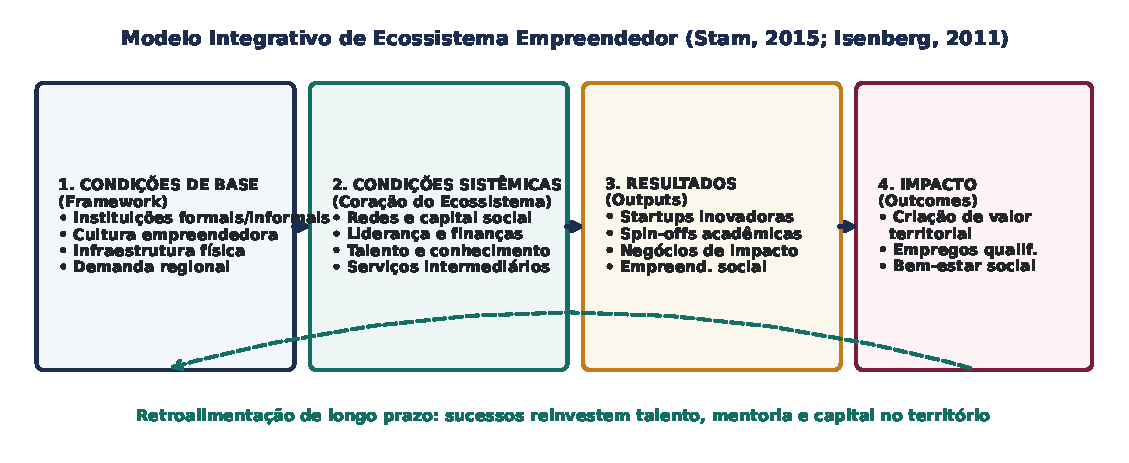
\includegraphics[width=0.94\textwidth]{figures/fig03_ecossistema_stam.pdf}
  \caption{Arquitetura multinível do Ecossistema Empreendedor segundo Stam \& van de Ven (2021) articulada aos seis domínios de Isenberg e às cinco dimensões da proximidade de Boschma (2005).}
  \label{fig:ecossistema_stam}
\end{figure}

\etapa{4}{Estudos de Caso e Aplicações Passo a Passo}

\begin{boxExemplo}{1}{Diagnóstico dos 6 Domínios de Isenberg e Efeito Gargalo}
\passoEnunciado{Uma equipe técnica avaliou os seis domínios de Isenberg em um polo regional do interior baiano (escala de $1{,}0$ a $10{,}0$), obtendo as seguintes notas: Capital Humano ($x_1 = 8{,}0$), Suporte/Universidades ($x_2 = 7{,}5$), Política ($x_3 = 6{,}0$), Cultura ($x_4 = 5{,}5$), Mercados ($x_5 = 5{,}0$) e Finanças/Capital de Risco ($x_6 = 1{,}5$).}
\passoDados{$x = (8{,}0;\; 7{,}5;\; 6{,}0;\; 5{,}5;\; 5{,}0;\; 1{,}5)$, com $n = 6$ domínios.}
\passoPedido{Calcular o índice pela média aritmética simples ($I_{\text{arit}}$) e pela média geométrica ($I_{\text{EE}}^{\text{geom}}$), explicando a diferença conceitual entre os resultados.}
\passoMetodo{Cálculo de $I_{\text{arit}} = \frac{1}{n}\sum x_i$ e $I_{\text{EE}}^{\text{geom}} = \left(\prod x_i\right)^{1/6}$.}
\passoContas{
  \begin{enumerate}[leftmargin=1.4em, itemsep=2pt]
    \item Média aritmética simples:
    \[
    I_{\text{arit}} = \frac{8{,}0 + 7{,}5 + 6{,}0 + 5{,}5 + 5{,}0 + 1{,}5}{6} = \frac{33{,}5}{6} \approx 5{,}58
    \]
    \item Produto dos seis domínios:
    \[
    \prod_{i=1}^{6} x_i = 8{,}0 \times 7{,}5 \times 6{,}0 \times 5{,}5 \times 5{,}0 \times 1{,}5
    \]
    \[
    8{,}0 \times 7{,}5 = 60{,}0; \quad 60{,}0 \times 6{,}0 = 360{,}0; \quad 360{,}0 \times 5{,}5 = 1.980{,}0; \quad 1.980{,}0 \times 5{,}0 = 9.900{,}0; \quad 9.900{,}0 \times 1{,}5 = 14.850{,}0
    \]
    \item Média geométrica (raiz sexta):
    \[
    I_{\text{EE}}^{\text{geom}} = (14.850{,}0)^{1/6} \approx 4{,}96
    \]
  \end{enumerate}
}
\passoResposta{$I_{\text{arit}} = 5{,}58$ e $I_{\text{EE}}^{\text{geom}} = 4{,}96$.}
\passoVerificacao{A média aritmética mascara a gravidade do gargalo financeiro ($1{,}5$), sugerindo um ecossistema mediano ($5{,}58$). A média geométrica penaliza o desequilíbrio ($4{,}96$). Se o território elevar Finanças de $1{,}5$ para $4{,}5$ (via fundos regionais ou subvenção), o produto triplica para $44.550$ e $I_{\text{EE}}^{\text{geom}}$ salta para $(44.550)^{1/6} \approx 5{,}95$, um ganho de quase $20\%$ no desempenho global atuando em um único gargalo.}
\end{boxExemplo}

\begin{boxExemplo}{2}{Modelo Integrativo de Stam \& van de Ven: Base vs. Sistêmicas}
\passoEnunciado{Na avaliação de dois municípios vizinhos (Município A e Município B) segundo o modelo de Stam \& van de Ven (2021), as médias das Condições de Base ($I_{\text{CB}}$) e das Condições Sistêmicas ($I_{\text{CS}}$), ambas em escala $0$--$10$, foram: Município A ($I_{\text{CB}} = 7{,}0$, $I_{\text{CS}} = 6{,}0$); Município B ($I_{\text{CB}} = 7{,}0$, $I_{\text{CS}} = 2{,}5$). Estima-se empiricamente que a taxa de \textit{output} empreendedor produtivo (EBTs por $100$ mil habitantes) siga a relação multiplicativa $O_{\text{EBT}} = 0{,}45 \times I_{\text{CB}} \times I_{\text{CS}}$.}
\passoDados{Município A: $I_{\text{CB},A} = 7{,}0$, $I_{\text{CS},A} = 6{,}0$. Município B: $I_{\text{CB},B} = 7{,}0$, $I_{\text{CS},B} = 2{,}5$. Coeficiente $k = 0{,}45$.}
\passoPedido{Calcular o \textit{output} esperado $O_{\text{EBT}}$ de cada município e a razão de desempenho entre A e B.}
\passoMetodo{Substituição direta na função de produção do ecossistema $O_{\text{EBT}} = 0{,}45 \times I_{\text{CB}} \times I_{\text{CS}}$.}
\passoContas{
  \begin{enumerate}[leftmargin=1.4em, itemsep=2pt]
    \item \textit{Output} do Município A:
    \[
    O_{\text{EBT},A} = 0{,}45 \times 7{,}0 \times 6{,}0 = 0{,}45 \times 42{,}0 = 18{,}90\text{ EBTs / 100 mil hab.}
    \]
    \item \textit{Output} do Município B:
    \[
    O_{\text{EBT},B} = 0{,}45 \times 7{,}0 \times 2{,}5 = 0{,}45 \times 17{,}5 = 7{,}875\text{ EBTs / 100 mil hab.}
    \]
    \item Razão de desempenho:
    \[
    \frac{O_{\text{EBT},A}}{O_{\text{EBT},B}} = \frac{18{,}90}{7{,}875} = 2{,}40\text{ vezes}
    \]
  \end{enumerate}
}
\passoResposta{$O_{\text{EBT},A} = 18{,}90$ e $O_{\text{EBT},B} = 7{,}875$ EBTs/$100$ mil hab. (Município A gera $2{,}40$ vezes mais EBTs).}
\passoVerificacao{Mesmo com condições de base idênticas ($I_{\text{CB}} = 7{,}0$, boa infraestrutura e segurança jurídica), a ausência de redes, liderança empreendedora e capital semente ($I_{\text{CS}} = 2{,}5$) reduz o resultado de B a menos da metade. Condições de base são necessárias, mas insuficientes sem ativação sistêmica.}
\end{boxExemplo}

\begin{boxExemplo}{3}{Ponto Ótimo da Proximidade Cognitiva (Boschma, 2005)}
\passoEnunciado{Em um programa de cooperação entre grupos de pesquisa universitários e pequenas indústrias de alimentos regionais, o desempenho inovador colaborativo ($P$, em índice de $0$ a $100$) em função da distância cognitiva $\Delta c \in [0, 10]$ é modelado pela curva em U invertido $P(\Delta c) = 24\,\Delta c - 3\,(\Delta c)^2$.}
\passoDados{$P(\Delta c) = 24\,\Delta c - 3\,(\Delta c)^2$, onde $\alpha = 24$ e $\beta = 3$.}
\passoPedido{Determinar a distância cognitiva ótima ($\Delta c^*$), o desempenho máximo $P(\Delta c^*)$ e comparar com dois casos extremos: excesso de proximidade ($\Delta c = 1$) e excesso de distância ($\Delta c = 7$).}
\passoMetodo{Derivação de $P(\Delta c)$ em relação a $\Delta c$ e igualação a zero ($\frac{dP}{d\Delta c} = 0$), seguida de avaliação pontual.}
\passoContas{
  \begin{enumerate}[leftmargin=1.4em, itemsep=2pt]
    \item Cálculo do ponto ótimo:
    \[
    \frac{dP}{d\Delta c} = 24 - 6\,\Delta c = 0 \implies 6\,\Delta c^* = 24 \implies \Delta c^* = 4{,}0
    \]
    \item Desempenho máximo em $\Delta c^* = 4{,}0$:
    \[
    P(4{,}0) = 24(4{,}0) - 3(4{,}0)^2 = 96 - 3(16) = 96 - 48 = 48{,}0
    \]
    \item Caso de excesso de proximidade ($\Delta c = 1{,}0$ — todos pensam igual):
    \[
    P(1{,}0) = 24(1{,}0) - 3(1{,}0)^2 = 24 - 3 = 21{,}0
    \]
    \item Caso de excesso de distância ($\Delta c = 7{,}0$ — falta linguagem comum):
    \[
    P(7{,}0) = 24(7{,}0) - 3(7{,}0)^2 = 168 - 3(49) = 168 - 147 = 21{,}0
    \]
  \end{enumerate}
}
\passoResposta{$\Delta c^* = 4{,}0$, com desempenho máximo $P(4{,}0) = 48{,}0$. Nos extremos ($\Delta c = 1$ ou $\Delta c = 7$), o desempenho cai para $21{,}0$ (redução de $56{,}25\%$).}
\passoVerificacao{O resultado comprova a tese de Boschma: nem a proximidade cognitiva absoluta ($\Delta c \to 0$, onde nada de novo se aprende), nem a distância extrema ($\Delta c \to 8$, onde cessa a comunicação) maximizam a inovação. A atuação de intermediários tecnológicos (NITs, consultores de extensão) serve justamente para calibrar $\Delta c$ próximo ao ponto ótimo.}
\end{boxExemplo}

\begin{boxExemplo}{4}{Paradoxo da Proximidade e Diagnóstico de \textit{Lock-in} em Rede Local}
\passoEnunciado{Uma incubadora territorial acompanha $20$ empresas de base tecnológica. Levantamento de redes mostrou que $16$ dessas empresas realizam $90\%$ de suas parcerias técnicas apenas com outras empresas da mesma cidade e ex-colegas da mesma graduação (alta proximidade social, geográfica e cognitiva), registrando taxa média de lançamento de novos produtos de $6\%$ ao ano. As outras $4$ empresas mantêm conexões híbridas com clientes e centros de pesquisa de outras regiões (proximidade balanceada), registrando taxa de $21\%$ ao ano.}
\passoDados{Grupo Fechado: $n_1 = 16$, taxa $= 6\%$/ano. Grupo Híbrido: $n_2 = 4$, taxa $= 21\%$/ano.}
\passoPedido{Calcular a taxa média ponderada de inovação do ecossistema atual e projetar a nova taxa caso políticas de conexão externa (missões técnicas e editais em rede) convertam metade do grupo fechado ($8$ empresas) para o perfil híbrido.}
\passoMetodo{Média ponderada $\bar{T} = \frac{n_1 t_1 + n_2 t_2}{n_1 + n_2}$.}
\passoContas{
  \begin{enumerate}[leftmargin=1.4em, itemsep=2pt]
    \item Taxa média atual ($n_1 = 16$, $n_2 = 4$):
    \[
    \bar{T}_{\text{atual}} = \frac{(16 \times 6\%) + (4 \times 21\%)}{20} = \frac{96\% + 84\%}{20} = \frac{180\%}{20} = 9{,}0\%\text{ ao ano}
    \]
    \item Taxa média após conversão de $8$ empresas ($n_1' = 8$, $n_2' = 12$):
    \[
    \bar{T}_{\text{proj}} = \frac{(8 \times 6\%) + (12 \times 21\%)}{20} = \frac{48\% + 252\%}{20} = \frac{300\%}{20} = 15{,}0\%\text{ ao ano}
    \]
    \item Ganho relativo sobre a taxa inicial:
    \[
    \Delta_{\text{rel}} = \frac{15{,}0 - 9{,}0}{9{,}0} \times 100\% = 66{,}67\%
    \]
  \end{enumerate}
}
\passoResposta{A taxa média do ecossistema sobe de $9{,}0\%$ para $15{,}0\%$ ao ano (aumento relativo de $66{,}67\%$).}
\passoVerificacao{O exercício quantifica o paradoxo da proximidade de Boschma: excesso de confiança fechada e homofilia acadêmica gera redundância informacional. Abrir ``pontes externas'' sem destruir o enraizamento local rompe o \textit{lock-in} cognitivo.}
\end{boxExemplo}

\begin{boxExemplo}{5}{Contraponto às \textit{Gazelles}: Retenção Territorial de Emprego e Renda}
\passoEnunciado{Um fundo estadual dispõe de $\reais{3.000.000}$ em fomento e analisa duas carteiras alternativas para $5$ anos: (A) apostar integralmente em $1$ startup \textit{gazelle} de plataforma digital urbana que gera $25$ empregos locais altamente remunerados ($\reais{8.000}$/mês médios), mas terceiriza $70\%$ de sua operação em nuvem internacional e planeja transferir a sede após a rodada Série A no ano $3$; (B) apoiar $10$ PMEs tecnológicas territoriais ($\reais{300.000}$ cada) em bioeconomia e automação regional que geram $8$ empregos diretos cada ($\reais{4.500}$/mês médios), permanecendo enraizadas pelos $5$ anos completos.}
\passoDados{Orçamento $= \reais{3.000.000}$; horizonte $= 60$ meses ($5$ anos); Opção A: $25$ empregos por $36$ meses a $\reais{8.000}$/mês; Opção B: $10 \times 8 = 80$ empregos por $60$ meses a $\reais{4.500}$/mês.}
\passoPedido{Calcular a massa salarial acumulada retida no território em cada opção ao longo dos $5$ anos e o custo público por emprego-ano gerado.}
\passoMetodo{Massa salarial $= N_{\text{emp}} \times W_{\text{mês}} \times M_{\text{meses}}$. Empregos-ano $= N_{\text{emp}} \times (\text{anos de permanência})$.}
\passoContas{
  \begin{enumerate}[leftmargin=1.4em, itemsep=2pt]
    \item Opção A (\textit{Gazelle}, $3$ anos $= 36$ meses no território):
    \[
    \text{Massa}_A = 25 \times 8.000 \times 36 = \reais{7.200.000}
    \]
    \[
    \text{Empregos-ano}_A = 25 \times 3 = 75\text{ empregos-ano} \implies \text{Custo} = \frac{3.000.000}{75} = \reais{40.000}\text{/emprego-ano}
    \]
    \item Opção B ($10$ PMEs enraizadas, $5$ anos $= 60$ meses):
    \[
    \text{Massa}_B = 80 \times 4.500 \times 60 = \reais{21.600.000}
    \]
    \[
    \text{Empregos-ano}_B = 80 \times 5 = 400\text{ empregos-ano} \implies \text{Custo} = \frac{3.000.000}{400} = \reais{7.500}\text{/emprego-ano}
    \]
  \end{enumerate}
}
\passoResposta{A Opção B retém $\reais{21.600.000}$ em massa salarial ($3{,}0$ vezes mais que a Opção A) a um custo de $\reais{7.500}$ por emprego-ano (contra $\reais{40.000}$ na Opção A).}
\passoVerificacao{Sem negar o papel das empresas de alto crescimento, os números expõem o risco de políticas periféricas focadas exclusivamente em \textit{gazelles} móveis: quando o capital e a sede migram após rodadas externas, o território subsidia a etapa de maior risco e perde os \textit{outcomes} de longo prazo.}
\end{boxExemplo}

\etapa{5}{Armadilhas Conceituais e Erros Mais Comuns}

\begin{boxErro}[Erro 1: Confundir Sistema Regional de Inovação (SRI) com Ecossistema Empreendedor (EE)]
Embora ambos tratem da dimensão territorial da inovação, o SRI coloca foco nas instituições de P\&D, universidades e firmas incumbentes, enquanto o EE coloca o empreendedor como agente central da criação de novos negócios. Tratar um parque tecnológico universitário sem empreendedores ativos como um EE maduro confunde infraestrutura acadêmica com dinamismo empreendedor.
\end{boxErro}

\begin{boxErro}[Erro 2: Usar Média Aritmética para Mascarar Gargalos Sistêmicos]
Em diagnósticos de ecossistemas (Isenberg e Stam), compensar uma nota péssima em Finanças ou Mercados com notas altas em Universidades via média aritmética esconde a trava estrutural do sistema. Um ecossistema funciona como cadeia multiplicativa: sem capital ou compradores iniciais, a pesquisa acadêmica não se converte em negócios sustentáveis.
\end{boxErro}

\begin{boxErro}[Erro 3: Assumir que ``Mais Proximidade'' é Sempre Melhor]
Um equívoco frequente em projetos de incubadoras e redes locais é supor que aproximar indefinidamente os atores maximiza a inovação. Como demonstrou Boschma (2005), proximidade cognitiva ou social excessiva gera redundância e \textit{lock-in}, exigindo abertura controlada a conhecimentos e parceiros externos.
\end{boxErro}

\begin{boxErro}[Erro 4: Importar Modelos de \textit{Gazelles} sem Leitura de Retenção Local]
Copiar métricas do Vale do Silício (número de unicórnios e rodadas de \textit{venture capital}) em regiões com baixa densidade financeira e cadeias agroindustriais tradicionais induz políticas que ignoram oportunidades reais de inovação incremental, bioeconomia e PMEs tecnológicas enraizadas.
\end{boxErro}

\etapa{6}{Lista de Exercícios (15 Questões Graduadas)}

\subsection*{Bloco A — Conceituais e Básicos (Questões 1 a 5)}

\begin{enumerate}[leftmargin=1.6em, itemsep=6pt]
  \item Explique a diferença central entre a abordagem dos Sistemas Regionais de Inovação (SRI) e a dos Ecossistemas Empreendedores (EE) quanto ao protagonista do processo inovativo.
  \espacoResolucao[1.8cm]

  \item Liste os seis domínios do Ecossistema Empreendedor de Daniel Isenberg (2011) e indique dois elementos concretos que compõem o domínio de \textit{Suporte}.
  \espacoResolucao[1.8cm]

  \item No modelo de Stam \& van de Ven (2021), diferencie \textit{condições de base}, \textit{condições sistêmicas}, \textit{outputs} e \textit{outcomes}.
  \espacoResolucao[1.8cm]

  \item Um ecossistema regional obteve notas $9{,}0$, $9{,}0$, $9{,}0$ e $1{,}0$ em quatro pilares analisados. Calcule a média aritmética e a média geométrica dessas notas e comente o efeito do pilar mais fraco.
  \espacoResolucao[1.8cm]

  \item Defina brevemente cada uma das cinco dimensões da proximidade propostas por Ron Boschma (2005).
  \espacoResolucao[1.8cm]
\end{enumerate}

\subsection*{Bloco B — Intermediários e Aplicados (Questões 6 a 10)}

\begin{enumerate}[leftmargin=1.6em, itemsep=6pt, resume]
  \item Em um diagnóstico territorial baseado em Stam \& van de Ven (2021), as Condições de Base receberam escore $I_{\text{CB}} = 8{,}0$ e as Condições Sistêmicas receberam $I_{\text{CS}} = 3{,}0$. Utilizando $O_{\text{EBT}} = 0{,}50 \times I_{\text{CB}} \times I_{\text{CS}}$, calcule o \textit{output} atual e o novo \textit{output} caso uma política de redes e capital semente eleve $I_{\text{CS}}$ para $5{,}5$.
  \espacoResolucao[2.2cm]

  \item Considere que o desempenho inovador de parcerias entre EBTs e cooperativas agrícolas siga a função $P(\Delta c) = 30\,\Delta c - 2{,}5\,(\Delta c)^2$, onde $\Delta c$ é a distância cognitiva ($0$ a $10$). Calcule a distância cognitiva ótima ($\Delta c^*$) e o desempenho máximo $P(\Delta c^*)$.
  \espacoResolucao[2.2cm]

  \item Explique como o excesso de proximidade social e institucional pode gerar \textit{lock-in} cognitivo em um polo tecnológico regional e proponha duas ações práticas para mitigar esse paradoxo.
  \espacoResolucao[2.0cm]

  \item Avalie criticamente a priorização exclusiva de empresas \textit{gazelles} em editais públicos estaduais no Nordeste brasileiro frente ao desenvolvimento territorial de médio e longo prazo.
  \espacoResolucao[2.0cm]

  \item Um município do interior apresenta forte proximidade geográfica e social entre suas empresas, mas baixa proximidade cognitiva com a universidade local ($\Delta c = 9{,}0$). Como a criação de um Núcleo de Inovação Tecnológica (NIT) ou escritório de extensão pode atuar sobre as dimensões de Boschma?
  \espacoResolucao[2.0cm]
\end{enumerate}

\subsection*{Bloco C — Questões Objetivas de Fixação (Questões 11 a 15)}

\begin{enumerate}[leftmargin=1.6em, itemsep=6pt, resume]
  \item No modelo de Ecossistema Empreendedor de Daniel Isenberg (2011), a tolerância ao fracasso honesto, a visibilidade de empreendedores locais e a aceitação social do risco pertencem ao domínio:
  \begin{alternativas}
    \item Política.
    \item Finanças.
    \item Cultura.
    \item Suporte.
    \item Mercados.
  \end{alternativas}

  \item No modelo integrativo de Stam (2015) e Stam \& van de Ven (2021), representam respectivamente uma \textbf{condição de base}, uma \textbf{condição sistêmica} e um \textbf{\textit{outcome}}:
  \begin{alternativas}
    \item Redes de mentoria, criação de startups e infraestrutura rodoviária.
    \item Instituições formais/segurança jurídica, financiamento/talento especializado e geração de valor agregado/bem-estar territorial.
    \item Capital de risco, cultura empreendedora e número de patentes depositadas.
    \item Demanda agregada, infraestrutura física e política monetária nacional.
    \item Serviços jurídicos, instituições formais e existência de parques tecnológicos.
  \end{alternativas}

  \item Segundo Ron Boschma (2005), a dimensão da proximidade que se refere ao grau em que dois atores compartilham bases de conhecimento e linguagem técnica suficientes para absorver e processar novas informações é a proximidade:
  \begin{alternativas}
    \item Geográfica.
    \item Social.
    \item Institucional.
    \item Cognitiva.
    \item Organizacional.
  \end{alternativas}

  \item Sobre o paradoxo da proximidade formulado por Boschma (2005), é correto afirmar que:
  \begin{alternativas}
    \item A distância cognitiva nula ($\Delta c = 0$) garante o maior volume possível de inovações radicais.
    \item A proximidade geográfica substitui integralmente todas as demais dimensões de proximidade.
    \item Tanto a ausência quanto o excesso de proximidade podem prejudicar a inovação, gerando falta de coordenação no primeiro caso e \textit{lock-in} no segundo.
    \item Redes sociais altamente fechadas impedem qualquer risco de acomodação ou redundância informacional.
    \item A proximidade institucional impede o surgimento de conflitos regulatórios ou de normas informais.
  \end{alternativas}

  \item Se quatro domínios de um ecossistema apresentam escores $4{,}0$, $4{,}0$, $9{,}0$ e $9{,}0$, sua média geométrica $I_{\text{EE}}^{\text{geom}}$ é exatamente igual a:
  \begin{alternativas}
    \item $5{,}5$
    \item $6{,}0$
    \item $6{,}5$
    \item $7{,}0$
    \item $7{,}5$
  \end{alternativas}
\end{enumerate}

\etapa{7}{Questões de Alta Complexidade (Estilo ANPAD / Pós-Graduação / CT\&I)}

\begin{enumerate}[leftmargin=1.6em, itemsep=8pt]
  \item \textbf{(Estilo Pós-Graduação / Desenvolvimento Territorial)} Considere as afirmações sobre Ecossistemas Empreendedores e Proximidades:
  \begin{itemize}[leftmargin=1.2em, itemsep=2pt]
    \item[I.] A existência de proximidade organizacional ou cognitiva forte permite que colaborações inovadoras ocorram mesmo entre atores geograficamente distantes, mostrando que a proximidade física não é condição absoluta.
    \item[II.] No modelo de Stam \& van de Ven (2021), as condições de base determinam isoladamente o surgimento de empresas de alto impacto, dispensando a formação de redes empreendedoras locais.
    \item[III.] Políticas de fomento voltadas exclusivamente a \textit{gazelles} podem subestimar o potencial multiplicador de PMEs tecnológicas enraizadas em cadeias produtivas regionais.
  \end{itemize}
  Está correto o que se afirma em:
  \begin{alternativas}
    \item I, apenas.
    \item II, apenas.
    \item I e III, apenas.
    \item II e III, apenas.
    \item I, II e III.
  \end{alternativas}

  \item \textbf{(Estilo ANPAD / Modelagem de Ecossistemas)} Um pesquisador modelou o desempenho colaborativo entre universidades e empresas em dois setores territoriais: no Setor Alfa, $P_A(\Delta c) = 18\,\Delta c - 1{,}5\,(\Delta c)^2$; no Setor Beta, $P_B(\Delta c) = 20\,\Delta c - 2{,}5\,(\Delta c)^2$. Comparando os pontos ótimos de distância cognitiva ($\Delta c^*$) e os respectivos desempenhos máximos ($P_{\max}$), conclui-se que:
  \begin{alternativas}
    \item $\Delta c_A^* = 6{,}0$ com $P_{A,\max} = 54{,}0$; $\Delta c_B^* = 4{,}0$ com $P_{B,\max} = 40{,}0$.
    \item $\Delta c_A^* = 4{,}0$ com $P_{A,\max} = 40{,}0$; $\Delta c_B^* = 6{,}0$ com $P_{B,\max} = 54{,}0$.
    \item $\Delta c_A^* = 12{,}0$ com $P_{A,\max} = 108{,}0$; $\Delta c_B^* = 8{,}0$ com $P_{B,\max} = 80{,}0$.
    \item Ambos possuem o mesmo ponto ótimo $\Delta c^* = 5{,}0$, variando apenas o nível máximo de desempenho.
    \item O Setor Beta apresenta maior desempenho máximo por tolerar maior distância cognitiva.
  \end{alternativas}

  \item \textbf{(Estilo Concurso CT\&I / Políticas de Inovação)} Um estado brasileiro investiu pesadamente na construção de prédios de parques tecnológicos (infraestrutura física) e na reforma de leis estaduais de desburocratização, mas após cinco anos registrou baixíssima taxa de criação de EBTs e saída precoce de startups para São Paulo. À luz de Isenberg (2011) e Stam (2015), a explicação mais precisa para esse resultado é:
  \begin{alternativas}
    \item A criação de infraestrutura física e legal (condições de base) é suficiente para gerar \textit{outputs}, indicando erro na mensuração estatística.
    \item A política concentrou-se em condições de base e infraestrutura sem ativar condições sistêmicas críticas como capital semente local, redes de mentoria empreendedora e mercados compradores regionais.
    \item O modelo de Isenberg recomenda eliminar as universidades do ecossistema para acelerar o surgimento de empresas.
    \item A saída de startups comprova que a proximidade institucional impede qualquer vínculo com investidores externos.
    \item O problema decorre exclusivamente do excesso de proximidade cognitiva entre os prédios do parque tecnológico.
  \end{alternativas}
\end{enumerate}

\begin{boxDica}[Contraponto Crítico e Prática Territorial (Conexão AV1 e AV3)]
Na \textbf{AV1}, ao comparar um ecossistema periférico com um polo metropolitano usando Isenberg ou Stam, evite diagnósticos genéricos do tipo ``falta apoio''. Identifique exatamente qual condição sistêmica (finanças, redes, mercados âncora) está agindo como gargalo multiplicativo. Na \textbf{AV3}, demonstre como seu empreendimento ou política utiliza as cinco proximidades de Boschma para conectar o saber acadêmico ao setor produtivo local sem cair em redes fechadas.
\end{boxDica}

\clearpage
\etapa{8}{Gabarito Comentado (Questões 1 a 18)}

\begin{boxGabarito}[Respostas Comentadas — Exercícios 1 a 15 e Questões de Alta Complexidade 16 a 18]
\begin{enumerate}[leftmargin=1.6em, itemsep=4pt]
  \item \textbf{Resposta:} O SRI foca na arquitetura institucional de geração e difusão de conhecimento (universidades, ICTs, políticas de P\&D e firmas estabelecidas), enquanto o EE coloca o empreendedor ambicioso como agente central, analisando como recursos e redes se articulam para criar e escalar negócios.
  \item \textbf{Resposta:} Os seis domínios de Isenberg são: Política, Finanças, Cultura, Suporte, Capital Humano e Mercados. Exemplos em \textit{Suporte}: infraestrutura física/digital (incubadoras, banda larga) e serviços especializados (contabilidade, advogados de PI).
  \item \textbf{Resposta:} Condições de base são os fundamentos estruturais (instituições, cultura, infraestrutura, demanda); condições sistêmicas são o motor ativo do ecossistema (redes, liderança, finanças, talento, conhecimento, intermediários); \textit{outputs} são as realizações empreendedoras (novas EBTs/inovações); \textit{outcomes} são os resultados finais de desenvolvimento (valor agregado, empregos e bem-estar territorial).
  \item \textbf{Resposta:} Média aritmética $= (9+9+9+1)/4 = 28/4 = 7{,}00$. Média geométrica $= (9 \times 9 \times 9 \times 1)^{1/4} = (729)^{1/4} = 27^{1/2} \approx 5{,}20$. A média geométrica reflete o efeito gargalo do pilar com nota $1{,}0$.
  \item \textbf{Resposta:} Geográfica (distância física); Cognitiva (base de conhecimento compartilhada); Organizacional (coordenação em arranjos formais/redes); Social (confiança e laços interpessoais); Institucional (normas formais e informais comuns).
  \item \textbf{Resposta:} Atual: $O_1 = 0{,}50 \times 8{,}0 \times 3{,}0 = 12{,}0$ EBTs/$100$ mil hab. Novo: $O_2 = 0{,}50 \times 8{,}0 \times 5{,}5 = 22{,}0$ EBTs/$100$ mil hab. (incremento de $83{,}3\%$).
  \item \textbf{Resposta:} $\frac{dP}{d\Delta c} = 30 - 5\,\Delta c = 0 \implies \Delta c^* = 6{,}0$. Desempenho máximo: $P(6{,}0) = 30(6) - 2{,}5(36) = 180 - 90 = 90{,}0$.
  \item \textbf{Resposta:} O excesso de proximidade social e institucional faz os atores repetirem rotinas e rejeitarem ideias externas (\textit{lock-in} cognitivo). Ações mitigadoras: editais obrigando parcerias inter-regionais e programas de intercâmbio técnico com outros ecossistemas.
  \item \textbf{Resposta:} Focar apenas em \textit{gazelles} pode drenar recursos escassos para poucos negócios que frequentemente migram de sede em busca de capital externo, enquanto PMEs tecnológicas locais geram mais empregos duradouros e retenção de renda regional.
  \item \textbf{Resposta:} O NIT atua como tradutor cognitivo e organizacional, reduzindo $\Delta c$ de $9{,}0$ para uma faixa funcional e criando pontes formais (contratos de P\&D, prestação de serviços) entre universidade e empresas locais.
  \item \textbf{Gabarito: (C).} Tolerância ao risco/fracasso e valorização do empreendedor compõem o domínio Cultura.
  \item \textbf{Gabarito: (B).} Instituições formais = condição de base; financiamento/talento = condição sistêmica; valor agregado/bem-estar = \textit{outcome}.
  \item \textbf{Gabarito: (D).} Proximidade cognitiva refere-se à base compartilhada de conhecimento e capacidade de absorção.
  \item \textbf{Gabarito: (C).} Tanto a distância excessiva quanto a proximidade excessiva prejudicam o desempenho inovador (curva em U invertido).
  \item \textbf{Gabarito: (B).} $(4 \times 4 \times 9 \times 9)^{1/4} = (16 \times 81)^{1/4} = 2 \times 3 = 6{,}0$.
  \item \textbf{Gabarito: (C).} A assertiva II é falsa pois condições de base precisam ser ativadas pelas condições sistêmicas.
  \item \textbf{Gabarito: (A).} Setor Alfa: $18 - 3\,\Delta c = 0 \implies \Delta c_A^* = 6{,}0$, $P_A(6) = 18(6) - 1{,}5(36) = 108 - 54 = 54{,}0$. Setor Beta: $20 - 5\,\Delta c = 0 \implies \Delta c_B^* = 4{,}0$, $P_B(4) = 20(4) - 2{,}5(16) = 80 - 40 = 40{,}0$.
  \item \textbf{Gabarito: (B).} Prédios e leis são condições de base/suporte; faltaram condições sistêmicas (capital, redes, compradores locais).
\end{enumerate}
\end{boxGabarito}

\begin{boxResumo}
\begin{itemize}[leftmargin=1.4em, itemsep=2pt]
  \item SRIs enfocam instituições de conhecimento e P\&D; Ecossistemas Empreendedores enfocam o empreendedor e a articulação dinâmica de recursos.
  \item Isenberg (2011) organiza o ecossistema em 6 domínios (Política, Finanças, Cultura, Suporte, Capital Humano e Mercados).
  \item Stam \& van de Ven (2021) distinguem condições de base e sistêmicas que geram \textit{outputs} empreendedores e \textit{outcomes} territoriais, capturados de forma não compensatória pela média geométrica.
  \item Boschma (2005) define 5 proximidades e alerta para o paradoxo da proximidade (\textit{lock-in}), complementado pela crítica à obsessão por \textit{gazelles}.
\end{itemize}
\end{boxResumo}

\begin{boxTeste}
Responda sem consultar o texto e confira o gabarito logo abaixo:
\begin{enumerate}[leftmargin=1.4em, itemsep=3pt]
  \item (\V\ / \F) No modelo de Stam \& van de Ven (2021), infraestrutura física e instituições formais são classificadas como condições sistêmicas.
  \item (\V\ / \F) Na curva em U invertido de Boschma, o máximo desempenho inovador ocorre em um nível intermediário de distância cognitiva.
  \item (\V\ / \F) A média geométrica é mais sensível a gargalos em um único domínio do ecossistema do que a média aritmética.
  \item (\V\ / \F) Políticas voltadas apenas para empresas \textit{gazelles} garantem automaticamente maior retenção salarial em territórios periféricos.
\end{enumerate}
\vspace{4pt}
\textbf{Gabarito do Checkpoint:} 1. \F\ (são condições de base); 2. \V; 3. \V; 4. \F\ (há risco de migração de sede e menor retenção territorial).
\end{boxTeste}

\chapter{Governança Territorial da Inovação e Políticas Públicas de CT\&I}
\label{cap:unid1_cap04}

\noindent\tagAV{AV1 (30\%)}\ \tagCritico

\vspace{6pt}

\begin{capObjetivos}
Ao concluir este capítulo, você deverá ser capaz de:
\begin{itemize}[leftmargin=1.4em, itemsep=3pt]
  \item Explicar a transição analítica da \textbf{Hélice Trípode} (Etzkowitz \& Leydesdorff) para os modelos de \textbf{Hélice Quádrupla} e \textbf{Hélice Quíntupla}, incorporando a sociedade civil e a transição socioecológica.
  \item Analisar o papel do \textbf{Estado Empreendedor} e das \textbf{Políticas Orientadas por Missões} (Mazzucato) no financiamento de risco tecnológico e na criação de mercados.
  \item Avaliar criticamente a eficácia de \textbf{habitats de inovação} (incubadoras, aceleradoras e parques tecnológicos), distinguindo ecossistemas enraizados de ``catedrais no deserto''.
  \item Interpretar e aplicar os principais instrumentos do \textbf{Marco Legal de CT\&I no Brasil} (Lei n.\textsuperscript{o} 10.973/2004, EC 85/2015, Lei n.\textsuperscript{o} 13.243/2016) e da \textbf{Lei do Bem} (Lei n.\textsuperscript{o} 11.196/2005).
  \item Formular críticas fundamentadas sobre a assimetria entre \textbf{socialização do risco e privatização dos ganhos} e sobre os riscos do \textbf{isomorfismo institucional} em políticas regionais.
\end{itemize}
\end{capObjetivos}

\begin{capRevisao}
No Capítulo~3, analisamos os Ecossistemas Empreendedores (Isenberg, Stam) e os Sistemas Regionais de Inovação (SRI), compreendendo como as cinco dimensões de proximidade de Boschma (cognitiva, organizacional, social, institucional e geográfica) condicionam a circulação de conhecimento. Neste Capítulo~4, damos um passo adiante para examinar \textbf{quem governa e quem financia} esses sistemas: as interações institucionais em hélice, os instrumentos jurídicos e fiscais de Ciência, Tecnologia e Inovação (CT\&I) e as tensões distributivas entre o setor público e o capital privado.
\end{capRevisao}

\etapa{3}{Fundamentação Teórica, Marco Legal e Modelagem}

\begin{boxSimbolo}[Vocabulário Conceitual e Símbolos do Capítulo]
\renewcommand{\arraystretch}{1.18}
\begin{tabular}{@{}p{2.4cm} p{12.0cm}@{}}
  $H_3, H_4, H_5$ & Modelos de Hélice Trípode, Quádrupla e Quíntupla de governança da inovação. \\
  $D_{P\&D}$ & Dispêndio total elegível em Pesquisa, Desenvolvimento e Inovação (em R\$). \\
  $\alpha_{excl}$ & Percentual de exclusão adicional na base de cálculo do IRPJ/CSLL (Lei do Bem). \\
  $\tau_{efetiva}$ & Alíquota tributária efetiva combinada de IRPJ e CSLL no regime de Lucro Real ($0{,}34$). \\
  $E_{LeiBem}$ & Economia fiscal líquida obtida via incentivos à P\&D da Lei n.\textsuperscript{o} 11.196/2005. \\
  $A_{pub}$ & Razão de alavancagem de investimento privado por unidade de recurso público ($I_{priv}/I_{pub}$). \\
  $E_{hab}$ & Índice de enraizamento territorial de um habitat de inovação ($0 \le E_{hab} \le 1$). \\
  ETEC / NIT & Encomenda Tecnológica / Núcleo de Inovação Tecnológica (Marco Legal de CT\&I). \\
\end{tabular}
\end{boxSimbolo}

\subsection{Da Hélice Trípode à Hélice Quádrupla e Quíntupla}

A governança da inovação territorial envolve a coordenação contínua de atores que operam sob lógicas institucionais distintas. Na formulação clássica de Henry Etzkowitz e Loet Leydesdorff, o modelo da \textbf{Hélice Trípode ($H_3$)} rompe com a visão linear de inovação (pesquisa básica $\to$ aplicada $\to$ mercado) ao propor uma dinâmica espiral de retroalimentação entre três esferas institucionais. Nessa arquitetura, a \textbf{Universidade} responde pela produção de conhecimento e formação avançada, a \textbf{Empresa} conduz a apropriação produtiva e a comercialização, e o \textbf{Governo} atua por meio da regulação, do fomento e do poder de compra. O elemento decisivo desse arranjo reside na sobreposição de papéis e na criação de organizações híbridas, de modo que universidades estruturam incubadoras e escritórios de transferência de tecnologia, empresas mantêm centros próprios de pesquisa e governos passam a operar como investidores de capital de risco.

\begin{boxConceito}[Evolução para a Hélice Quádrupla ($H_4$) e Quíntupla ($H_5$)]
Embora a Hélice Trípode explique com precisão a dinâmica de clusters industriais tradicionais, sua formulação original tende a negligenciar os usuários finais, os movimentos sociais e os limites ecológicos do território. Para superar essa restrição analítica, Carayannis e Campbell propuseram duas ampliações estruturais do modelo. A \textbf{Hélice Quádrupla ($H_4$)} incorpora a \textbf{sociedade civil organizada}, a cultura, a mídia e os usuários-cidadãos como quarta esfera de governança, fazendo com que a inovação seja coproduzida por meio de laboratórios vivos (\textit{living labs}), demandas sociais territorializadas e legitimação democrática das prioridades tecnológicas. Em um passo adicional, a \textbf{Hélice Quíntupla ($H_5$)} integra o \textbf{ambiente natural e a transição socioecológica} como quinta hélice, convertendo a crise climática, a conservação hídrica e a biodiversidade em vetores centrais que orientam e restringem a P\&D territorial.
\end{boxConceito}

Quando essas cinco esferas se articulam no território, as decisões tecnológicas deixam de responder apenas a critérios de eficiência industrial isolada e passam a incorporar legitimidade social e sustentabilidade ambiental. A Figura~\ref{fig:helice_quintupla} esquematiza essa arquitetura integrada, destacando os fluxos de conhecimento e governança entre Universidade, Empresa, Estado, Sociedade Civil e Transição Socioecológica.

\begin{figure}[H]
  \centering
  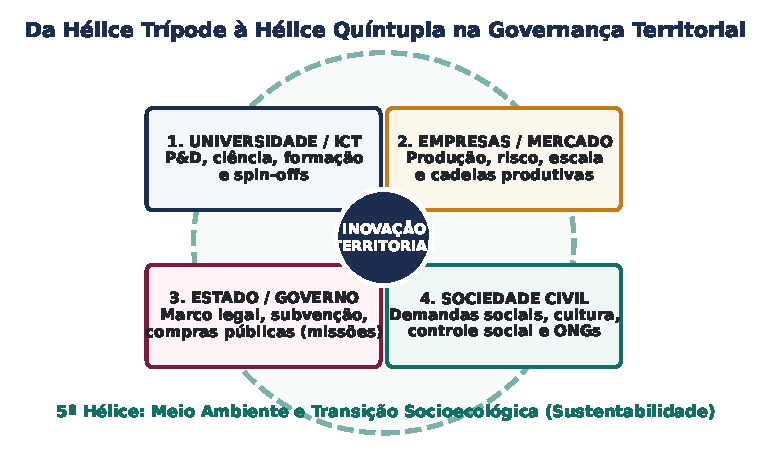
\includegraphics[width=0.90\textwidth]{figures/fig04_helice_quintupla.pdf}
  \caption{Modelo integrado da Hélice Quíntupla: articulação entre Universidade, Empresa, Estado, Sociedade Civil e Transição Socioecológica na governança territorial da inovação.}
  \label{fig:helice_quintupla}
\end{figure}

\subsection{Estado Empreendedor e Políticas Orientadas por Missões}

Na teoria econômica neoclássica convencional, a intervenção estatal em CT\&I justifica-se apenas para corrigir \textit{falhas de mercado}, como as externalidades positivas da pesquisa básica e as assimetrias de informação. Mariana Mazzucato contesta essa visão minimalista ao evidenciar que as grandes ondas tecnológicas contemporâneas (internet, GPS, telas sensíveis ao toque, biotecnologia e energias renováveis) dependeram de um \textbf{Estado Empreendedor}, isto é, de um setor público disposto a assumir a \textbf{incerteza radical} nos estágios iniciais da inovação, quando o capital privado e o \textit{venture capital} ainda se recusam a entrar devido ao longo prazo de maturação e ao elevado risco técnico.

Complementarmente, as \textbf{Políticas Orientadas por Missões} propõem organizar os instrumentos de CT\&I em torno de desafios territoriais concretos e mensuráveis, como a descarbonização de cadeias produtivas, a segurança hídrica no Semiárido ou a bioeconomia amazônica. Ao definir problemas públicos específicos como eixo coordenador, o poder público substitui a distribuição indiferenciada de subsídios horizontais por metas estratégicas com direcionalidade clara, mobilizando múltiplos setores e atores locais em torno de soluções verificáveis.

\subsection{Habitats de Inovação: Sucesso Territorial vs. ``Catedrais no Deserto''}

Incubadoras de empresas, aceleradoras e parques tecnológicos constituem \textbf{habitats de inovação} destinados a reduzir custos de transação e acelerar a maturação de empreendimentos intensivos em conhecimento. Contudo, a literatura de economia regional alerta para o fenômeno das \textbf{``catedrais no deserto''}, caracterizado por grandes complexos imobiliários financiados com recursos públicos em regiões desprovidas de base produtiva aderente, massa crítica de pesquisadores ou demanda empresarial local.

Sem densidade cognitiva nem encadeamentos produtivos regionais, as empresas graduadas nesses espaços tendem a migrar para metrópoles em busca de mercado e fornecedores especializados, drenando o investimento público municipal. Para evitar esse isolamento, o parque tecnológico ou a incubadora exige \textbf{enraizamento territorial}, que se efetiva mediante conexão orgânica com as cadeias produtivas locais, presença de âncoras demandantes e mecanismos concretos de retenção de talentos e empresas no próprio território.

\subsection{Marco Legal de CT\&I no Brasil e Lei do Bem}

O arcabouço jurídico brasileiro de incentivo à inovação evoluiu nas últimas duas décadas para reduzir a insegurança jurídica na interação entre universidades e empresas. O ponto de inflexão iniciou-se com a \textbf{Lei de Inovação (Lei n.\textsuperscript{o} 10.973/2004)}, que instituiu os Núcleos de Inovação Tecnológica (NITs) nas Instituições Científicas, Tecnológicas e de Inovação (ICTs), regulamentou o compartilhamento de laboratórios públicos e autorizou a subvenção econômica direta a empresas. Na sequência, a \textbf{Lei do Bem (Lei n.\textsuperscript{o} 11.196/2005, Cap. III)} criou incentivos fiscais automáticos, dispensando aprovação prévia de projeto e exigindo apenas prestação de contas posterior ao MCTI, para empresas tributadas pelo \textbf{Lucro Real} que realizem dispêndios em P\&D\&I, permitindo exclusão adicional de 60\% a 100\% desses gastos na apuração do IRPJ e da CSLL.

Esse conjunto normativo foi aprofundado pela \textbf{Emenda Constitucional n.\textsuperscript{o} 85/2015} e pelo \textbf{Novo Marco Legal de CT\&I (Lei n.\textsuperscript{o} 13.243/2016, regulamentada pelo Decreto n.\textsuperscript{o} 9.283/2018)}, que constitucionalizou o Sistema Nacional de CT\&I e simplificou procedimentos de compras para pesquisa. Além disso, o Novo Marco autorizou a participação minoritária do Estado no capital de empresas de base tecnológica e consolidou a \textbf{Encomenda Tecnológica (ETEC)}, instrumento que permite ao poder público contratar diretamente o esforço de P\&D de soluções com risco tecnológico, mesmo quando o resultado final ainda é incerto.

\begin{boxConceito}[Contraponto Crítico: Socialização do Risco e Isomorfismo Institucional]
Duas patologias recorrentes comprometem a eficácia das políticas territoriais de CT\&I. A primeira consiste na \textbf{socialização do risco com privatização dos ganhos}, situação em que o Estado financia a pesquisa básica e absorve a incerteza inicial, mas entrega a propriedade intelectual e os lucros futuros integralmente ao setor privado sem cláusulas de retorno, tais como \textit{royalties}, participação acionária, licenciamento acessível ou contrapartidas territoriais. A segunda patologia refere-se ao \textbf{isomorfismo institucional}, isto é, à tendência de gestores públicos replicarem acriticamente modelos de regiões centrais (como o Vale do Silício ou Cambridge) em territórios periféricos ou semiáridos, ignorando a estrutura produtiva local e gerando estruturas burocráticas ociosas.
\end{boxConceito}

\begin{boxFormula}[Modelagem Quantitativa da Lei do Bem e do Enraizamento de Habitats]
\textbf{1. Economia Fiscal Efetiva pela Lei do Bem (Lucro Real):}
Para uma empresa com lucro tributável sujeito à alíquota combinada de IRPJ (15\% + adicional de 10\%) e CSLL (9\%), totalizando $\tau_{efetiva} = 0{,}34$, a economia tributária adicional decorrente da exclusão incentivada de dispêndios em P\&D é:
\[
E_{LeiBem} = D_{P\&D} \times \alpha_{excl} \times \tau_{efetiva}
\]
onde $\alpha_{excl} = 0{,}60$ (regra geral), podendo receber acréscimo de $+0{,}20$ se houver incremento superior a 5\% no número de pesquisadores dedicados exclusivamente à P\&D (totalizando $0{,}80$), ou $+0{,}10$ se o incremento for de até 5\%, além de $+0{,}20$ caso haja patente concedida ou cultivar registrada (chegando a $\alpha_{excl} = 1{,}00$).

\vspace{4pt}
\textbf{2. Alavancagem de Fomento Público e Índice de Enraizamento de Habitat:}
\[
A_{pub} = \frac{I_{priv}}{I_{pub}} \qquad \text{e} \qquad E_{hab} = \left(\frac{E_{locais}}{E_{total}}\right) \times \left(\frac{C_{locais}}{C_{total}}\right)
\]
Em que $E_{locais}/E_{total}$ é a proporção de empresas graduadas que permanecem sediadas no território após 3 anos, e $C_{locais}/C_{total}$ é a fração de compras de insumos e serviços tecnológicos contratados junto a fornecedores regionais.
\end{boxFormula}

\etapa{4}{Exemplos Resolvidos e Estudos de Caso Comentados}

\begin{boxExemplo}{4.1}{Mapeamento da Hélice Quíntupla no Semiárido Baiano}
\passoEnunciado{Um consórcio intermunicipal do Semiárido baiano pretende estruturar um programa de inovação para a cadeia da caprinocultura leiteira e forragicultura adaptada à seca, evitando o modelo tradicional de pacotes tecnológicos importados.}
\passoDados{Participam: (i) universidade pública estadual com laboratório de genética e nutrição animal; (ii) 45 pequenas agroindústrias e laticínios regionais; (iii) secretaria estadual de ciência e tecnologia e banco regional de fomento; (iv) associações de agricultores familiares e sindicatos rurais; (v) plano estadual de convivência com o Semiárido e combate à desertificação.}
\passoPedido{Classificar cada ator segundo o modelo da Hélice Quíntupla ($H_5$) e identificar o risco caso a quarta e a quinta hélices sejam excluídas da governança.}
\passoMetodo{Aplicação analítica do modelo de Carayannis, Barth e Campbell ($H_5$), mapeando as cinco esferas institucionais e suas interfaces de retroalimentação.}
\passoContas{
Mapeamento das cinco hélices no território:
\begin{itemize}[leftmargin=1.4em, itemsep=2pt]
  \item \textbf{Hélice 1 (Academia):} Universidade estadual (P\&D em manejo forrageiro e melhoramento genético).
  \item \textbf{Hélice 2 (Empresa):} Laticínios e agroindústrias locais (processamento, logística e comercialização).
  \item \textbf{Hélice 3 (Estado):} Secretaria de CT\&I e banco de fomento (crédito direcionado, assistência técnica e compras públicas institucionais).
  \item \textbf{Hélice 4 (Sociedade Civil):} Associações de agricultores familiares (validação participativa das tecnologias e legitimidade social).
  \item \textbf{Hélice 5 (Transição Socioecológica):} Agenda de convivência com o Semiárido (uso racional de água, conservação da Caatinga e energia solar rural).
\end{itemize}
}
\passoResposta{Todas as cinco hélices estão representadas. A exclusão da Hélice 4 geraria rejeição por inadequação cultural e produtiva; a exclusão da Hélice 5 induziria sobrepastejo e esgotamento hídrico.}
\passoVerificacao{O diagnóstico demonstra coerência territorial: no Semiárido, a sustentabilidade ecológica (Hélice 5) e a organização comunitária (Hélice 4) são condições de viabilidade econômica, e não meros apêndices.}
\end{boxExemplo}

\begin{boxExemplo}{4.2}{Cálculo de Benefício Fiscal pela Lei do Bem (Lei n.\textsuperscript{o} 11.196/2005)}
\passoEnunciado{Uma empresa baiana de biotecnologia agrícola, tributada pelo Lucro Real e com lucro fiscal positivo, investiu em pesquisa para bioinsumos adaptados ao cerrado e ao semiárido.}
\passoDados{Dispêndio elegível em P\&D no ano-base: $D_{P\&D} = \reais{1.200.000,00}$. A empresa ampliou sua equipe exclusiva de pesquisadores em $8\%$ em relação ao ano anterior (acima do gatilho de $5\%$), não possuindo ainda patente concedida no período. Alíquota combinada efetiva de IRPJ e CSLL: $\tau_{efetiva} = 0{,}34$.}
\passoPedido{Calcular o percentual total de exclusão adicional ($\alpha_{excl}$), a economia fiscal líquida ($E_{LeiBem}$) e o custo líquido efetivo do investimento em P\&D após o incentivo.}
\passoMetodo{Aplicação direta da equação de economia fiscal da Lei do Bem: $E_{LeiBem} = D_{P\&D} \times \alpha_{excl} \times \tau_{efetiva}$.}
\passoContas{
1. Percentual de exclusão adicional:
\[
\alpha_{excl} = 0{,}60\ (\text{base}) + 0{,}20\ (\text{incremento de pesquisadores } > 5\%) = 0{,}80\ (80\%)
\]
2. Economia fiscal adicional (além da dedução normal como despesa operacional):
\[
E_{LeiBem} = 1.200.000 \times 0{,}80 \times 0{,}34 = 960.000 \times 0{,}34 = \reais{326.400,00}
\]
3. Note-se que, como despesa operacional dedutível, o dispêndio já reduz o imposto em $1.200.000 \times 0{,}34 = \reais{408.000,00}$. Somando a dedução normal à exclusão incentivada ($E_{LeiBem}$), a redução tributária total atinge $\reais{734.400,00}$, reduzindo o custo líquido desembolsado pela empresa para $\reais{465.600,00}$ ($38{,}8\%$ do valor original).
}
\passoResposta{Exclusão adicional $\alpha_{excl} = 80\%$; economia fiscal incentivada $E_{LeiBem} = \reais{326.400,00}$.}
\passoVerificacao{O resultado reflete o limite legal da Lei do Bem para empresas no Lucro Real com lucro tributável. Em empresas iniciantes (\textit{startups}) no Simples Nacional ou em prejuízo fiscal, esse incentivo não é utilizável, exigindo outros instrumentos como subvenção econômica.}
\end{boxExemplo}

\begin{boxExemplo}{4.3}{Diagnóstico de ``Catedral no Deserto'' em Parques Tecnológicos}
\passoEnunciado{Dois municípios do interior brasileiro inauguraram parques tecnológicos há cinco anos. O gestor estadual precisa comparar o desempenho territorial dos dois habitats para decidir a renovação de aportes públicos.}
\passoDados{
\textbf{Parque A:} Investimento público acumulado $I_{pub} = \reais{40\text{ milhões}}$; investimento privado atraído $I_{priv} = \reais{12\text{ milhões}}$; de $20$ empresas graduadas, apenas $4$ permaneceram no território ($E_{locais} = 4$); fração de compras locais de serviços e insumos $C_{locais}/C_{total} = 0{,}15$.\\
\textbf{Parque B:} $I_{pub} = \reais{25\text{ milhões}}$; $I_{priv} = \reais{50\text{ milhões}}$; de $22$ empresas graduadas, $18$ permaneceram no território; fração de compras locais $C_{locais}/C_{total} = 0{,}65$.
}
\passoPedido{Calcular a razão de alavancagem $A_{pub}$ e o índice de enraizamento $E_{hab}$ de ambos os parques, diagnosticando qual deles se configura como ``catedral no deserto''.}
\passoMetodo{Cálculo comparativo via $A_{pub} = I_{priv}/I_{pub}$ e $E_{hab} = (E_{locais}/E_{total}) \times (C_{locais}/C_{total})$.}
\passoContas{
\textbf{Parque A:}
\[
A_{pub, A} = \frac{12}{40} = 0{,}30 \qquad \text{e} \qquad E_{hab, A} = \left(\frac{4}{20}\right) \times 0{,}15 = 0{,}20 \times 0{,}15 = 0{,}030\ (3{,}0\%)
\]
\textbf{Parque B:}
\[
A_{pub, B} = \frac{50}{25} = 2{,}00 \qquad \text{e} \qquad E_{hab, B} = \left(\frac{18}{22}\right) \times 0{,}65 \approx 0{,}8182 \times 0{,}65 \approx 0{,}5318\ (53{,}2\%)
\]
}
\passoResposta{O Parque A apresenta baixa alavancagem ($0{,}30$) e enraizamento residual ($E_{hab} = 3{,}0\%$), caracterizando-se como ``catedral no deserto''. O Parque B alavanca $2{,}00$ reais privados por real público e retém mais de metade do efeito multiplicador ($E_{hab} = 53{,}2\%$).}
\passoVerificacao{A diferença expressiva mostra que infraestrutura física sem encadeamento produtivo local gera fuga de empresas graduadas para metrópoles, drenando o investimento público municipal.}
\end{boxExemplo}

\begin{boxExemplo}{4.4}{Encomenda Tecnológica (ETEC) para Segurança Hídrica}
\passoEnunciado{Um município do Polígono das Secas enfrenta salinização de poços artesianos. As tecnologias comerciais disponíveis têm custo energético proibitivo para comunidades rurais isoladas. A prefeitura decide utilizar o instrumento de Encomenda Tecnológica (ETEC), previsto na Lei n.\textsuperscript{o} 13.243/2016.}
\passoDados{Orçamento total de P\&D estimado para desenvolver um protótipo de dessalinizador solar de baixo custo: $\reais{2.000.000,00}$. Pelo contrato de compartilhamento de risco tecnológico, o poder público remunera $80\%$ dos custos de desenvolvimento conforme entregas de marcos técnicos e a \textit{startup} contratada assume $20\%$ como risco próprio, recebendo direito à encomenda em escala caso atinja a meta de eficiência.}
\passoPedido{Determinar o aporte máximo de risco assumido pelo Estado e pela \textit{startup}, explicando por que a licitação convencional por menor preço falharia nesse caso.}
\passoMetodo{Análise jurídico-econômica da ETEC (art. 20 da Lei n.\textsuperscript{o} 10.973/2004, alterado pela Lei n.\textsuperscript{o} 13.243/2016) e repartição contratual de risco.}
\passoContas{
1. Parcela de risco tecnológico assumida pelo ente público:
\[
R_{Estado} = 2.000.000 \times 0{,}80 = \reais{1.600.000,00}
\]
2. Parcela de contrapartida/risco assumida pela \textit{startup}:
\[
R_{Startup} = 2.000.000 \times 0{,}20 = \reais{400.000,00}
\]
Na licitação tradicional por menor preço, pressupõe-se que o objeto já exista pronto no mercado. Como a solução demanda P\&D com risco de insucesso técnico, nenhum fornecedor sério assumiria preço fixo sem margem proibitiva; a ETEC permite pagar pelo esforço de pesquisa validado por marcos, mesmo diante de incerteza.
}
\passoResposta{O Estado assume $\reais{1.600.000,00}$ ($80\%$) e a \textit{startup} assume $\reais{400.000,00}$ ($20\%$) do risco de desenvolvimento, viabilizando uma missão pública territorial.}
\passoVerificacao{Esse desenho concretiza o conceito de Estado Empreendedor e compras públicas para inovação, vinculando o gasto público a uma demanda real do território.}
\end{boxExemplo}

\begin{boxExemplo}{4.5}{Socialização do Risco vs. Privatização dos Ganhos}
\passoEnunciado{Uma agência pública de fomento aportou capital não reembolsável em uma empresa privada para o desenvolvimento de um software de monitoramento agrícola por satélite.}
\passoDados{Aporte público a fundo perdido: $I_{pub} = \reais{5.000.000,00}$. Após a validação da tecnologia, a empresa alcançou receita acumulada de $\reais{60.000.000,00}$ em 5 anos e Valor Presente Líquido privado de $\reais{25.000.000,00}$. Compare o Cenário 1 (contrato sem cláusula de retorno financeiro ao fundo público) com o Cenário 2 (contrato com cláusula de \textit{royalty} contingente ao sucesso comercial de $3\%$ sobre a receita bruta).}
\passoPedido{Calcular o retorno financeiro direto ao fundo público e a taxa de recuperação do aporte público em ambos os cenários.}
\passoMetodo{Cálculo do fluxo de retorno contratual ($R_{pub} = r \times \text{Receita}$) e da razão de recuperação ($R_{pub}/I_{pub}$).}
\passoContas{
\textbf{Cenário 1 (sem cláusula de retorno):}
\[
R_{pub, 1} = \reais{0,00} \implies \text{Recuperação} = 0\%
\]
\textbf{Cenário 2 (com \textit{royalty} contingente de $3\%$ sobre $\reais{60\text{ milhões}}$):}
\[
R_{pub, 2} = 60.000.000 \times 0{,}03 = \reais{1.800.000,00} \implies \text{Recuperação} = \frac{1.800.000}{5.000.000} = 0{,}36\ (36\%)
\]
}
\passoResposta{No Cenário 1 ocorre privatização integral dos ganhos ($0\%$ de retorno direto ao fundo). No Cenário 2, o fundo recupera $\reais{1.800.000,00}$ ($36\%$ do aporte), permitindo reinvestimento em novas missões territoriais sem inviabilizar o lucro privado.}
\passoVerificacao{Mecanismos como \textit{royalties} contingentes ao sucesso ou participação acionária pública (\textit{equity}) mitigam a assimetria apontada por Mazzucato, mantendo o fundo de inovação sustentável.}
\end{boxExemplo}

\etapa{5}{Armadilhas Conceituais e Erros Mais Comuns}

\begin{boxErro}[Erro 1: Confundir Hélice Quádrupla/Quíntupla com ``Mais Burocracia'']
Incluir sociedade civil ($H_4$) e transição socioecológica ($H_5$) não significa criar conselhos meramente consultivos e lentos. Significa incorporar a \textbf{demanda social} e a \textbf{restrição ecológica} na fase de concepção tecnológica, evitando que o projeto fracasse por rejeição comunitária ou inviabilidade ambiental na fase de difusão.
\end{boxErro}

\begin{boxErro}[Erro 2: Aplicar a Lei do Bem a Empresas do Simples Nacional ou Lucro Presumido]
Um erro técnico recorrente em projetos de consultoria é prometer economia fiscal via Lei n.\textsuperscript{o} 11.196/2005 para \textit{startups} recém-criadas. A Lei do Bem exige obrigatoriamente apuração pelo \textbf{Lucro Real} e existência de lucro fiscal no exercício; empresas em prejuízo ou no Simples Nacional não usufruem desse benefício.
\end{boxErro}

\begin{boxErro}[Erro 3: Reduzir o Estado Empreendedor a ``Gasto Público Sem Critério'']
Defender o Estado Empreendedor não equivale a aprovar subsídios incondicionais. A proposta de Mazzucato exige \textbf{direcionalidade por missões}, monitoramento de metas técnicas e mecanismos de compartilhamento de retornos quando o risco assumido pelo setor público gera lucros extraordinários.
\end{boxErro}

\begin{boxErro}[Erro 4: Replicar Parques Tecnológicos por Isomorfismo Institucional]
Construir prédios espelhados com salas de \textit{coworking} em municípios sem massa crítica científica nem vocação produtiva articulada cria apenas custos fixos de manutenção. O hardware (infraestrutura) nunca substitui o software institucional (confiança, demanda qualificada e capital humano).
\end{boxErro}

\etapa{6}{Exercícios Propostos (Básicos, Intermediários e Objetivos)}

\textbf{Parte A, Exercícios Básicos (Conceituação e Identificação)}

\textbf{1.} Diferencie, em até cinco linhas, o papel da Universidade e do Estado no modelo linear de inovação em comparação ao modelo da Hélice Trípode ($H_3$).
\espacoResolucao[1.8cm]

\textbf{2.} Explique por que a transição da Hélice Trípode ($H_3$) para a Hélice Quíntupla ($H_5$) é estratégica para territórios com alta vulnerabilidade climática, como o Semiárido nordestino.
\espacoResolucao[1.8cm]

\textbf{3.} Cite três instrumentos jurídicos introduzidos ou fortalecidos pelo Novo Marco Legal de CT\&I (Lei n.\textsuperscript{o} 13.243/2016) que facilitam a cooperação entre ICTs públicas e empresas.
\espacoResolucao[1.8cm]

\textbf{4.} Uma empresa optante pelo Lucro Presumido investiu $\reais{500.000,00}$ em P\&D e solicita o benefício fiscal da Lei do Bem. O pedido é juridicamente válido? Justifique.
\espacoResolucao[1.8cm]

\textbf{5.} Defina o conceito de ``catedral no deserto'' aplicado a parques tecnológicos e indique duas condições necessárias para evitá-la.
\espacoResolucao[1.8cm]

\textbf{Parte B, Exercícios Intermediários (Modelagem e Análise Quantitativa)}

\textbf{6.} Uma indústria farmacêutica no Lucro Real investiu $D_{P\&D} = \reais{2.500.000,00}$ em pesquisa de fitoterápicos nativos. A empresa não aumentou seu quadro de pesquisadores, mas obteve uma patente concedida no exercício, elevando $\alpha_{excl}$ para $0{,}80$ ($60\%$ base + $20\%$ patente). Com $\tau_{efetiva} = 0{,}34$, calcule a economia fiscal incentivada ($E_{LeiBem}$).
\espacoResolucao[2.0cm]

\textbf{7.} Um polo de inovação recebeu $\reais{15\text{ milhões}}$ de recursos públicos e atraiu $\reais{45\text{ milhões}}$ de investimento privado. Das $30$ empresas incubadas e graduadas, $21$ permanecem operando no município e realizam $50\%$ de suas compras de serviços na região. Calcule $A_{pub}$ e $E_{hab}$ e interprete o resultado.
\espacoResolucao[2.0cm]

\textbf{8.} Analise uma política pública estadual que concede subvenção econômica integral ($100\%$ a fundo perdido) para empresas estrangeiras instalarem centros de dados no território, sem exigência de contratação de pesquisadores locais nem transferência tecnológica para universidades regionais. Avalie à luz dos conceitos de \textit{enraizamento} e \textit{socialização do risco}.
\espacoResolucao[2.0cm]

\textbf{9.} Uma prefeitura deseja contratar o desenvolvimento de um sistema de alerta inteligente de enchentes com sensores ainda não disponíveis comercialmente. Compare os prós e contras de utilizar um pregão eletrônico tradicional versus uma Encomenda Tecnológica (ETEC).
\espacoResolucao[2.0cm]

\textbf{10.} Elabore o desenho sintético de uma \textbf{Política Orientada por Missões} para o seu território (ou para a Região Metropolitana de Feira de Santana), especificando: (a) o grande desafio territorial, (b) a missão mensurável com prazo, e (c) os instrumentos de fomento e poder de compra mobilizados.
\espacoResolucao[2.0cm]

\textbf{Parte C, Questões Objetivas (Estilo Exame / Concurso, A a E)}

\textbf{11.} Sobre a evolução dos modelos de Hélice de inovação (Etzkowitz, Leydesdorff, Carayannis e Campbell), assinale a alternativa \textbf{correta}:
\begin{alternativas}
  \item A Hélice Trípode exclui o setor público da dinâmica inovativa, restringindo-o à cobrança de tributos.
  \item A Hélice Quádrupla substitui as universidades pela mídia digital como principal produtora de conhecimento científico.
  \item A Hélice Quíntupla integra o ambiente natural e a transição socioecológica como dimensões estruturantes da governança da inovação.
  \item Na Hélice Trípode, as esferas institucionais atuam de forma estanque, sendo vedada a criação de organizações híbridas como os NITs.
  \item O modelo de Hélice Quíntupla aplica-se exclusivamente a países de alta renda com matriz energética nuclear.
\end{alternativas}

\textbf{12.} No debate econômico proposto por Mariana Mazzucato em \textit{O Estado Empreendedor}, a atuação estatal nas fases iniciais de tecnologias disruptivas caracteriza-se principalmente por:
\begin{alternativas}
  \item Limitar-se à correção de falhas de mercado após a consolidação comercial da tecnologia pelo capital privado.
  \item Assumir a incerteza radical por meio de financiamento paciente e compras públicas estratégicas, moldando e criando novos mercados.
  \item Substituir integralmente o empreendedorismo privado em todas as etapas de comercialização varejista.
  \item Eliminar a necessidade de proteção de propriedade intelectual em favor da desregulamentação tributária absoluta.
  \item Concentrar recursos apenas em empréstimos de curto prazo com taxas de juros superiores às de mercado.
\end{alternativas}

\textbf{13.} Em relação ao Marco Legal de CT\&I no Brasil (Lei n.\textsuperscript{o} 10.973/2004, EC 85/2015 e Lei n.\textsuperscript{o} 13.243/2016) e à Lei do Bem (Lei n.\textsuperscript{o} 11.196/2005), é \textbf{correto} afirmar que:
\begin{alternativas}
  \item A Lei do Bem permite que microempresas do Simples Nacional deduzam até $100\%$ de seus gastos de P\&D no imposto de renda.
  \item A Encomenda Tecnológica (ETEC) só pode ser utilizada para a compra de equipamentos padronizados de prateleira pelo critério de menor preço.
  \item Os Núcleos de Inovação Tecnológica (NITs) são proibidos por lei de negociar contratos de licenciamento de patentes com o setor privado.
  \item A Lei n.\textsuperscript{o} 13.243/2016 ampliou a segurança jurídica para o compartilhamento de laboratórios de ICTs públicas com empresas e para a realização de ETECs em projetos com risco tecnológico.
  \item A EC 85/2015 retirou da Constituição Federal a competência dos estados e municípios para legislar e fomentar sistemas locais de inovação.
\end{alternativas}

\textbf{14.} Uma empresa tributada pelo Lucro Real realiza dispêndio elegível de $\reais{1.000.000,00}$ em P\&D, enquadrando-se na exclusão adicional básica de $60\%$ da Lei do Bem ($\alpha_{excl} = 0{,}60$). Considerando $\tau_{efetiva} = 34\%$, o valor da economia fiscal adicional ($E_{LeiBem}$) proporcionada exclusivamente pelo incentivo da Lei do Bem é de:
\begin{alternativas}
  \item $\reais{170.000,00}$
  \item $\reais{204.000,00}$
  \item $\reais{340.000,00}$
  \item $\reais{544.000,00}$
  \item $\reais{600.000,00}$
\end{alternativas}

\textbf{15.} O fenômeno do \textit{isomorfismo institucional} em políticas regionais de CT\&I manifesta-se quando:
\begin{alternativas}
  \item Um território adapta instrumentos de fomento às suas vocações produtivas endógenas e à sua biodiversidade.
  \item Agências de fomento exigem cláusulas de retorno público (\textit{royalties}) proporcionais ao risco tecnológico assumido.
  \item Gestores locais copiam formatos institucionais de ecossistemas hegemônicos (como parques tecnológicos genéricos) sem aderência à base econômica e social do território.
  \item Cooperativas agrícolas utilizam a Encomenda Tecnológica para desenvolver máquinas adaptadas à agricultura familiar.
  \item Universidades regionais reorganizam seus NITs para priorizar demandas de cadeias produtivas locais.
\end{alternativas}

\etapa{7}{Questões Autorais Estilo Pós-Graduação e Concursos}

\textbf{16. (Estilo ENADE / Pós-Graduação em Políticas Públicas)} Analise criticamente a seguinte afirmação: \textit{``A criação de um parque tecnológico de alto padrão arquitetônico e a concessão de isenções fiscais genéricas são condições suficientes para transformar uma região periférica em um polo de inovação dinâmica.''} Fundamente sua resposta com os conceitos de Hélice Quíntupla, ``catedrais no deserto'' e isomorfismo institucional.
\espacoResolucao[2.2cm]

\textbf{17. (Estilo Concurso para Analista em CT\&I, FINEP/FAPs)} Uma fundação estadual de amparo à pesquisa (FAP) financiou a fundo perdido o desenvolvimento de um novo bioinseticida em parceria entre uma universidade estadual e uma empresa privada. Cinco anos depois, a empresa vendeu a patente para uma multinacional e desativou a planta fabril no estado. Proponha três mecanismos contratuais e de governança, amparados pelo Marco Legal de CT\&I e pela abordagem de Mazzucato, que poderiam ter evitado a socialização do risco com privatização integral dos ganhos e perda territorial.
\espacoResolucao[2.2cm]

\textbf{18. (Estilo Mestrado Profissional, PPGPT/UEFS)} Um município baiano pretende estruturar um sistema local de inovação para a cadeia da mandioca e derivados (farinha especial, fécula biodegradável e bioembalagens). Redija uma proposta de governança em Hélice Quíntupla indicando: (i) os atores de cada uma das cinco hélices; (ii) um instrumento do Marco Legal de CT\&I aplicável; e (iii) dois indicadores quantitativos para monitorar o enraizamento territorial do programa.
\espacoResolucao[2.2cm]

\begin{boxDica}[Contraponto Crítico e Preparação para a AV1 (30\%)]
Ao analisar políticas públicas de CT\&I no seu fichamento crítico ou seminário da \textbf{AV1}, evite avaliações puramente descritivas (``a lei existe e cria incentivos''). Pergunte sempre: \textbf{quem acessa o instrumento} (grandes empresas no Lucro Real ou cooperativas e \textit{startups} locais?), \textbf{quem assume o risco inicial} e \textbf{qual parcela do valor gerado permanece retida no território}.
\end{boxDica}

\clearpage
\etapa{8}{Gabarito Comentado dos 18 Exercícios}

\begin{boxGabarito}[Respostas Comentadas: Capítulo 4]
\textbf{1.} No modelo linear, a universidade gera ciência básica isoladamente e o Estado apenas financia pesquisas sem interação direta. Na Hélice Trípode ($H_3$), Universidade, Empresa e Estado sobrepõem esferas, criando organizações híbridas (NITs, incubadoras, fundos de risco) em interação contínua.

\textbf{2.} A Hélice Quíntupla incorpora a sociedade civil ($H_4$) e a transição socioecológica ($H_5$). No Semiárido, inovações que ignoram o balanço hídrico, a conservação da Caatinga e a organização comunitária tendem à degradação ambiental e à baixa adoção social.

\textbf{3.} Entre os principais instrumentos: (i) Encomenda Tecnológica (ETEC); (ii) compartilhamento de laboratórios e infraestrutura de ICTs com empresas; (iii) permissão para participação minoritária do poder público no capital social de empresas inovadoras e simplificação da gestão financeira pelos NITs.

\textbf{4.} Não é válido. O benefício fiscal da Lei do Bem (Cap. III da Lei n.\textsuperscript{o} 11.196/2005) restringe-se a pessoas jurídicas tributadas pelo regime do \textbf{Lucro Real} que apurem lucro fiscal no período.

\textbf{5.} ``Catedral no deserto'' é um habitat de inovação (ex.: parque tecnológico) com alto investimento imobiliário público, porém desconectado do tecido produtivo local. Para evitá-la, exige-se demanda empresarial/pública aderente e articulação densa com ICTs e cadeias locais.

\textbf{6.} $E_{LeiBem} = 2.500.000 \times 0{,}80 \times 0{,}34 = \reais{680.000,00}$.

\textbf{7.} $A_{pub} = 45 / 15 = 3{,}00$ (cada real público alavancou $\reais{3,00}$ privados). $E_{hab} = (21/30) \times 0{,}50 = 0{,}70 \times 0{,}50 = 0{,}35$ ($35\%$). O habitat apresenta forte alavancagem privada e retenção territorial moderada-alta.

\textbf{8.} A política promove socialização do risco (subsídio integral público) com baixa retenção territorial: centros de dados operam com pouca mão de obra local e, sem contrapartida de P\&D regional ou transferência tecnológica, funcionam como enclaves desconectados do território.

\textbf{9.} O pregão eletrônico exige especificação fechada e produto pronto, inviabilizando soluções inéditas ou induzindo sobrepreço pelo risco. A ETEC permite contratar o esforço de P\&D com risco tecnológico compartilhado e marcos de entrega, ainda que exija maior capacidade técnica de fiscalização do gestor público.

\textbf{10.} Resposta aberta estruturada: deve definir um desafio territorial concreto (ex.: gestão de resíduos sólidos industriais ou eficiência hídrica), uma meta quantificável com prazo (ex.: reduzir em $40\%$ o descarte inadequado em 5 anos) e combinar fomento à P\&D com compras públicas (ETEC).

\textbf{11. (C)} A Hélice Quíntupla amplia a Hélice Quádrupla ao inserir o ambiente natural e a sustentabilidade socioecológica no centro da governança inovativa.

\textbf{12. (B)} Mazzucato demonstra que o Estado Empreendedor assume a incerteza radical e cria mercados por meio de financiamento paciente e missões, não se limitando a corrigir falhas residuais.

\textbf{13. (D)} A Lei n.\textsuperscript{o} 13.243/2016 consolidou a segurança jurídica para compartilhamento de infraestrutura de ICTs e para a contratação via ETEC. (A) exige Lucro Real; (B) ETEC é para risco tecnológico; (C) NITs têm essa atribuição; (E) EC 85 fortaleceu competências subnacionais.

\textbf{14. (B)} $E_{LeiBem} = 1.000.000 \times 0{,}60 \times 0{,}34 = \reais{204.000,00}$.

\textbf{15. (C)} Isomorfismo institucional ocorre quando se copiam modelos externos (como parques tecnológicos genéricos) sem adequação à estrutura produtiva e institucional local.

\textbf{16.} A afirmação é falsa. Infraestrutura física e isenções genéricas não criam densidade cognitiva nem demanda qualificada; sem conexão com a base produtiva, com a sociedade civil ($H_4$) e com a sustentabilidade ($H_5$), reproduz-se o isomorfismo institucional e criam-se ``catedrais no deserto''.

\textbf{17.} Três mecanismos: (i) cláusula de \textit{royalties} contingentes ao sucesso comercial revertidos ao fundo estadual; (ii) cláusula de permanência produtiva territorial ou preferência de licenciamento local em caso de transferência de controle; (iii) participação acionária minoritária ou bônus de subscrição pública, além de retenção de co-titularidade da PI pela ICT pública via NIT.

\textbf{18.} Academia: universidade/instituto federal (biotecnologia de amidos e bioplásticos); Empresa: casas de farinha modernizadas e indústrias de embalagens; Estado: prefeitura/governo estadual (ETEC ou subvenção FAP); Sociedade Civil: cooperativas de mandiocultores; Transição Socioecológica: substituição de plásticos fósseis e aproveitamento da manipueira. Indicadores sugeridos: $A_{pub}$ e $E_{hab}$ (ou taxa de retenção de valor local).
\end{boxGabarito}

\begin{boxResumo}
\begin{itemize}[leftmargin=1.4em, itemsep=3pt]
  \item A governança territorial evoluiu da \textbf{Hélice Trípode} (Universidade--Empresa--Estado) para a \textbf{Quádrupla} (+ Sociedade Civil) e a \textbf{Quíntupla} (+ Transição Socioecológica).
  \item O \textbf{Estado Empreendedor} assume incerteza radical e orienta políticas por \textbf{missões}, evitando subsídios sem direcionalidade.
  \item No Brasil, o \textbf{Marco Legal de CT\&I} (Leis 10.973/2004 e 13.243/2016) e a \textbf{Lei do Bem} (11.196/2005, exclusiva do Lucro Real) oferecem instrumentos complementares de cooperação e fomento.
  \item Políticas territoriais devem evitar o \textbf{isomorfismo institucional} (``catedrais no deserto'') e a assimetria entre \textbf{socialização do risco e privatização dos ganhos}.
\end{itemize}
\end{boxResumo}

\begin{boxTeste}
Julgue os itens a seguir como Verdadeiros (\V) ou Falsos (\F):
\begin{enumerate}[leftmargin=1.6em, itemsep=3pt]
  \item (\quad) A Hélice Quíntupla acrescenta o ambiente natural e a transição socioecológica como eixo estruturante da inovação territorial.
  \item (\quad) Empresas enquadradas no Simples Nacional podem utilizar a exclusão adicional de $60\%$ a $100\%$ da Lei do Bem no cálculo de seus tributos.
  \item (\quad) A Encomenda Tecnológica (ETEC) permite que o poder público contrate diretamente soluções com risco tecnológico em que o resultado final ainda é incerto.
  \item (\quad) O índice de enraizamento $E_{hab}$ será baixo mesmo que um parque tecnológico tenha alto investimento público, caso as empresas graduadas migrem para fora do território.
\end{enumerate}
\textbf{Gabarito do Checkpoint:} 1. \V \quad 2. \F \text{ (exige Lucro Real)} \quad 3. \V \quad 4. \V
\end{boxTeste}

\chapter{Empreendedorismo Social e Negócios de Impacto Territorial}
\label{cap:unid1_cap05}

\noindent\tagAV{AV1 (30\%)}\ \tagCritico

\vspace{6pt}

\begin{capObjetivos}
Ao concluir este capítulo, você deverá ser capaz de:
\begin{itemize}[leftmargin=1.4em, itemsep=3pt]
  \item Aplicar o \textbf{Quadro PCDO} (Austin, Stevenson \& Wei-Skillern, 2006) para contrastar o empreendedorismo comercial e o empreendedorismo social em suas dimensões estruturais.
  \item Avaliar empreendimentos segundo os critérios nacionais dos \textbf{Negócios de Impacto} (Aliança pelos Investimentos e Negócios de Impacto).
  \item Construir e quantificar uma \textbf{Teoria da Mudança} (Insumos $\to$ Atividades $\to$ \textit{Outputs} $\to$ \textit{Outcomes} $\to$ Impacto), calculando o \textbf{SROI} com ajuste de peso morto e deslocamento.
  \item Analisar o \textbf{Espectro do Capital} e instrumentos financeiros híbridos, como \textbf{Títulos de Impacto Social (SIBs)} e \textbf{\textit{Blended Finance}}.
  \item Diagnosticar o risco de \textbf{\textit{mission drift}} (desvio de missão) e problematizar a \textbf{financeirização do social} e os limites do hibridismo organizacional.
\end{itemize}
\end{capObjetivos}

\begin{capRevisao}
No Capítulo~4, discutimos como o Estado Empreendedor, os NITs e as políticas orientadas por missões criam condições macroinstitucionais para a inovação. Contudo, muitas falhas sociais e ambientais nos territórios não são resolvidas apenas por agências estatais ou por empresas orientadas exclusivamente ao lucro acionário. Neste Capítulo~5, investigamos as organizações híbridas que buscam equacionar sustentabilidade financeira e transformação socioambiental mensurável.
\end{capRevisao}

\etapa{3}{Fundamentação Teórica, Teoria da Mudança e Modelagem}

\begin{boxSimbolo}[Vocabulário Conceitual e Símbolos do Capítulo]
\renewcommand{\arraystretch}{1.18}
\begin{tabular}{@{}p{2.4cm} p{12.0cm}@{}}
  PCDO & Quadro analítico: \textit{People} (Pessoas), \textit{Context} (Contexto), \textit{Deal} (Negócio) e \textit{Opportunity} (Oportunidade), articulados pela Proposição de Valor Social (SVP). \\
  \textit{Outputs} & Produtos ou entregas diretas e imediatas das atividades (ex.: cisternas instaladas). \\
  \textit{Outcomes} & Mudanças ou benefícios reais percebidos pelo público-alvo (ex.: redução de doenças hídricas). \\
  $SROI$ & Retorno Social sobre o Investimento (\textit{Social Return on Investment}). \\
  $DW,\ DL$ & Fatores de ajuste de impacto: \textit{Deadweight} (peso morto) e \textit{Displacement} (deslocamento). \\
  $k_{blend}$ & Custo médio ponderado de capital em operações de \textit{Blended Finance}. \\
  SIBs & \textit{Social Impact Bonds} (Títulos / Contratos de Impacto Social com pagamento por resultado). \\
  \textit{Mission Drift} & Desvio gradual da missão social em favor de metas financeiras ou públicos de maior renda. \\
\end{tabular}
\end{boxSimbolo}

\subsection{O Quadro PCDO: Empreendedorismo Comercial vs. Social}

Em trabalho seminal, James Austin, Howard Stevenson e Jane Wei-Skillern (2006) adaptaram o modelo de empreendedorismo de Sahlman para explicar o que distingue o empreendedorismo social do comercial. O \textbf{Quadro PCDO} organiza essa análise ao articular quatro variáveis interdependentes, correspondentes a \textbf{Pessoas} (\textit{People}), \textbf{Contexto} (\textit{Context}), \textbf{Negócio ou Acordo} (\textit{Deal}) e \textbf{Oportunidade} (\textit{Opportunity}), tendo no centro a \textbf{Proposição de Valor Social (SVP)}. Enquanto no empreendimento comercial os contratos entre sócios, investidores e clientes tendem a ser padronizados pelo retorno financeiro, no empreendimento social a SVP precisa alinhar beneficiários que muitas vezes não têm capacidade de pagamento integral com terceiros financiadores, como o Estado, doadores ou clientes de subsídio cruzado.

\renewcommand{\arraystretch}{1.20}
\small
\begin{tabularx}{\textwidth}{@{}p{2.4cm} X X@{}}
  \toprule
  \rowcolor{etIndigo}
  \textcolor{white}{\bfseries Dimensão} & \textcolor{white}{\bfseries Empreendedorismo Comercial} & \textcolor{white}{\bfseries Empreendedorismo Social} \\
  \midrule
  \textbf{Oportunidade (O)} & Mercado em crescimento capaz de gerar retorno econômico apropriável. & Falha de mercado ou vulnerabilidade socioambiental persistente (demanda social). \\
  \rowcolor{bgGray}
  \textbf{Pessoas (P)} & Remuneração competitiva de mercado e participação acionária (\textit{equity}) para atrair talentos. & Mobilização de recursos humanos frequentemente dependente de propósito, voluntariado e redes comunitárias. \\
  \textbf{Contexto (C)} & Regulação setorial, juros e concorrência de mercado. & Marco regulatório público, políticas sociais, cultura territorial e vulnerabilidade institucional. \\
  \rowcolor{bgGray}
  \textbf{Negócio / Deal (D)} & Acordos contratuais padronizados entre investidores, sócios e clientes pagantes. & Relações complexas com múltiplos \textit{stakeholders} (beneficiários frequentemente distintos dos pagadores). \\
  \bottomrule
\end{tabularx}
\normalsize

\subsection{Critérios dos Negócios de Impacto}

No Brasil, a \textbf{Aliança pelos Investimentos e Negócios de Impacto} estabelece quatro pilares articulados para diferenciar um Negócio de Impacto genuíno de ações filantrópicas ou de práticas isoladas de responsabilidade social corporativa. O primeiro pilar é a \textbf{intencionalidade}, segundo a qual o propósito explícito de resolver um problema socioambiental consta na estratégia central da organização. O segundo exige uma \textbf{atividade-fim geradora de impacto}, garantindo que o benefício coletivo decorra diretamente do produto ou serviço principal comercializado, sem se restringir a doações acessórias de parte do lucro.

Além desses dois critérios de propósito, o empreendimento precisa estruturar um \textbf{modelo de negócio financeiramente sustentável}, capaz de gerar receitas próprias (via venda a usuários, empresas ou poder público) que cubram os custos operacionais e permitam ganhar escala sem dependência perpétua de doações. Complementando essa arquitetura, o quarto pilar combina \textbf{impacto mensurável e governança}, exigindo métricas claras de acompanhamento de resultados e mecanismos estatutários que protejam a missão social ao longo do tempo diante de pressões comerciais.

\subsection{Teoria da Mudança e Espectro do Capital}

A \textbf{Teoria da Mudança (ToC)} explicita a cadeia causal pela qual os recursos mobilizados geram transformação territorial, conforme representado no encadeamento a seguir.
\[
\textbf{Insumos} \longrightarrow \textbf{Atividades} \longrightarrow \textbf{\textit{Outputs} (Entregas)} \longrightarrow \textbf{\textit{Outcomes} (Resultados)} \longrightarrow \textbf{Impacto Sistêmico}
\]
Enquanto os \textit{outputs} medem o volume operacional produzido pela organização, como o número de oficinas ministradas ou de kits solares entregues, os \textit{outcomes} mensuram a mudança efetiva na vida do público atendido, expressa no aumento da renda líquida familiar, na redução de internações ou na autonomia energética.

No financiamento dessas iniciativas, o \textbf{Espectro do Capital} posiciona as fontes de recursos em um contínuo que vai desde a \textbf{filantropia tradicional}, voltada exclusivamente ao retorno social com aceitação de perda total do principal, passando por investimentos \textbf{\textit{impact-first}} (que priorizam o impacto e aceitam retorno financeiro abaixo do mercado) e \textbf{\textit{finance-first}} (que exigem retorno de mercado com tese de impacto), até o \textbf{investimento tradicional} focado exclusivamente no retorno ajustado ao risco. A Figura~\ref{fig:teoria_mudanca_espectro} ilustra essa articulação entre a cadeia causal da Teoria da Mudança e o posicionamento dos instrumentos financeiros ao longo do Espectro do Capital.

\begin{figure}[H]
  \centering
  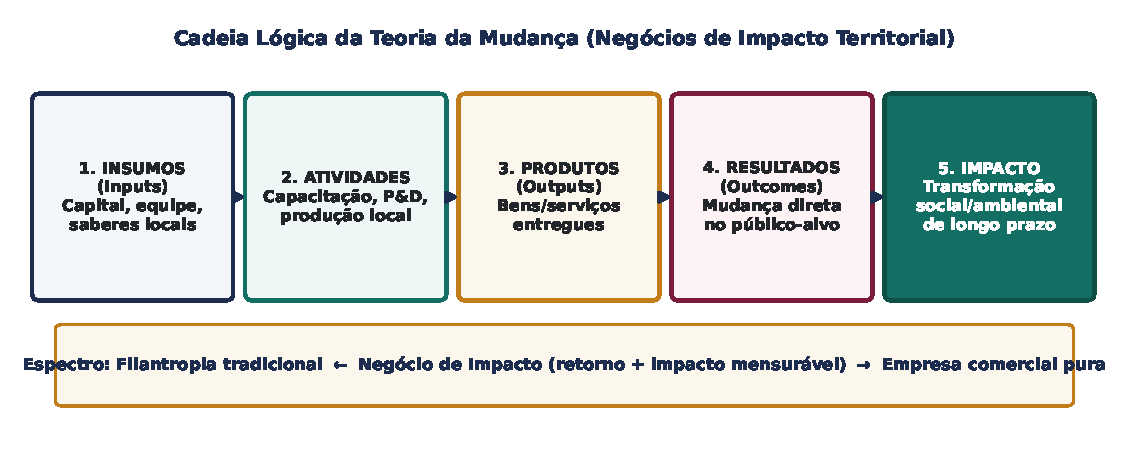
\includegraphics[width=0.94\textwidth]{figures/fig05_teoria_mudanca_espectro.pdf}
  \caption{Integração entre a cadeia causal da Teoria da Mudança e o posicionamento dos instrumentos financeiros ao longo do Espectro do Capital.}
  \label{fig:teoria_mudanca_espectro}
\end{figure}

\subsection{Instrumentos Financeiros Híbridos e Contraponto Crítico}

Dois instrumentos financeiros híbridos ganham destaque na agenda contemporânea de impacto por conectarem diferentes faixas do Espectro do Capital. O primeiro é o \textbf{\textit{Blended Finance} (Finanças Mistas)}, que combina estrategicamente capital concessional ou filantrópico (capaz de absorver primeiras perdas ou aceitar juros zero) com capital comercial privado, reduzindo o risco percebido e destravando investimentos em setores ou territórios periféricos. O segundo instrumento corresponde aos \textbf{Títulos de Impacto Social (SIBs / Contratos de Impacto Social)}, arranjo contratual em que investidores privados financiam antecipadamente uma intervenção social executada por um operador especializado, cabendo ao poder público reembolsar o investidor com remuneração pactuada apenas se metas independentes de \textit{outcome} forem comprovadamente atingidas.

\begin{boxConceito}[Contraponto Crítico: \textit{Mission Drift}, Financeirização do Social e Limites do Hibridismo]
A literatura crítica aponta três tensões estruturais que acompanham os negócios de impacto. A primeira é o \textbf{\textit{Mission Drift} (Desvio de Missão)}, que ocorre quando, diante da pressão de investidores por liquidez e margem, a empresa híbrida migra gradualmente para clientes de maior poder aquisitivo e abandona o público vulnerável de menor capacidade de pagamento. A segunda tensão envolve a \textbf{financeirização do social}, uma vez que os SIBs podem transformar direitos sociais constitucionais (educação, saúde, saneamento) em ativos financeiros sujeitos à lógica de retorno de curto prazo e à seleção adversa (\textit{cream-skimming}, priorizando casos mais fáceis de atingir a meta). A terceira tensão envolve os \textbf{limites do hibridismo}, pois nem todo problema territorial comporta um modelo de receita pagante; em situações de extrema pobreza ou provisão de bens públicos puros, a ação estatal direta e a economia solidária permanecem insubstituíveis.
\end{boxConceito}

\begin{boxFormula}[Modelagem Quantitativa: SROI Ajustado e Custo Ponderado em \textit{Blended Finance}]
\textbf{1. Valor de Impacto Líquido e Retorno Social sobre o Investimento ($SROI$):}
Para evitar superestimar o impacto atribuindo ao projeto mudanças que ocorreriam de qualquer maneira (\textit{deadweight}, $DW$) ou que apenas transferiram o problema para outro local (\textit{displacement}, $DL$), calcula-se o benefício líquido ajustado:
\[
V_{liq} = V_{bruto} \times (1 - DW) \times (1 - DL)
\]
A razão $SROI$ e o $SROI$ líquido percentual são dados por:
\[
SROI_{razao} = \frac{V_{liq}}{I_{total}} \qquad \text{e} \qquad SROI_{liq} = \frac{V_{liq} - I_{total}}{I_{total}}
\]

\textbf{2. Custo Médio Ponderado de Capital em \textit{Blended Finance} ($k_{blend}$):}
Sendo $w_i$ a fração de capital da camada $i$ (com $\sum w_i = 1$) e $k_i$ seu respectivo custo anual:
\[
k_{blend} = \sum_{i=1}^{n} w_i \cdot k_i
\]
\end{boxFormula}

\etapa{4}{Exemplos Resolvidos e Estudos de Caso Comentados}

\begin{boxExemplo}{5.1}{Aplicação do Quadro PCDO: \textit{Fintech} Urbana vs. Banco Comunitário Digital}
\passoEnunciado{Compare uma \textit{fintech} comercial de crédito pessoal em capital metropolitano com uma \textit{fintech} de impacto territorial voltada a microempreendedoras informais no Recôncavo Baiano.}
\passoDados{A \textit{fintech} comercial opera com garantia em folha ou histórico de crédito formal, captando em fundos de \textit{venture capital}. O negócio de impacto utiliza dados alternativos de comércio local, agentes comunitários de crédito e capital inicial subsidiado.}
\passoPedido{Estruturar a comparação pelas quatro dimensões do Quadro PCDO (Austin et al., 2006) e identificar a principal vulnerabilidade do negócio de impacto.}
\passoMetodo{Mapeamento comparativo qualitativo nas dimensões Oportunidade, Pessoas, Contexto e \textit{Deal}.}
\passoContas{
\begin{itemize}[leftmargin=1.4em, itemsep=2pt]
  \item \textbf{Oportunidade:} comercial busca margem sobre tomadores bancarizados; impacto busca inclusão produtiva de desbancarizados com redução de juros extorsivos.
  \item \textbf{Pessoas:} comercial remunera com \textit{stock options} de mercado; impacto combina equipe técnica com agentes locais remunerados por vínculo territorial.
  \item \textbf{Contexto:} impacto depende de regulação do Banco Central para sociedades de crédito direto e da informalidade da renda rural/urbana local.
  \item \textbf{Negócio (\textit{Deal}):} comercial tem relação bilateral investidor--cliente; impacto precisa conciliar retorno ao fundo concessional com taxas acessíveis às microempreendedoras.
\end{itemize}
}
\passoResposta{A principal vulnerabilidade do negócio de impacto no Quadro PCDO reside no \textit{Deal}: se o custo de captação subir, há pressão para elevar os juros às tomadoras, desencadeando \textit{mission drift}.}
\passoVerificacao{O Quadro PCDO explicita por que métricas comerciais padrão não capturam a complexidade de contratos com múltiplos interesses territoriais.}
\end{boxExemplo}

\begin{boxExemplo}{5.2}{Teoria da Mudança e Cálculo de SROI Ajustado em Saneamento Rural}
\passoEnunciado{Um negócio de impacto instalou sistemas modulares de tratamento de água cinza (biofiltros) em 200 residências rurais de um território semiárido, permitindo reuso agrícola em quintais produtivos.}
\passoDados{Investimento total do ciclo: $I_{total} = \reais{500.000,00}$. A valoração monetária bruta dos benefícios em 3 anos (economia de água comprada em carro-pipa, produção de hortaliças e redução de gastos com doenças de veiculação hídrica) somou $V_{bruto} = \reais{1.600.000,00}$. Auditoria independente estimou peso morto (\textit{deadweight}) de $DW = 20\%$ e efeito de deslocamento (\textit{displacement}) de $DL = 10\%$.}
\passoPedido{Distinguir um \textit{output} de um \textit{outcome} do projeto e calcular o benefício líquido ajustado ($V_{liq}$), o $SROI_{razao}$ e o $SROI_{liq}$.}
\passoMetodo{Aplicação da cadeia de Teoria da Mudança e das fórmulas de $SROI$ com descontos multiplicativos de $DW$ e $DL$.}
\passoContas{
1. Distinção causal: \textit{output} = 200 biofiltros instalados; \textit{outcome} = redução da incidência de diarreia infantil e aumento da segurança alimentar via reuso.\\
2. Benefício líquido ajustado:
\[
V_{liq} = 1.600.000 \times (1 - 0{,}20) \times (1 - 0{,}10) = 1.600.000 \times 0{,}80 \times 0{,}90 = 1.600.000 \times 0{,}72 = \reais{1.152.000,00}
\]
3. Indicadores de $SROI$:
\[
SROI_{razao} = \frac{1.152.000}{500.000} = 2{,}304 \approx 2{,}30 \qquad \text{e} \qquad SROI_{liq} = \frac{1.152.000 - 500.000}{500.000} = \frac{652.000}{500.000} = 1{,}304\ (130{,}4\%)
\]
}
\passoResposta{Cada $\reais{1,00}$ investido gerou $\reais{2,30}$ de valor socioambiental líquido ($SROI$ líquido de $130{,}4\%$).}
\passoVerificacao{O desconto de $28\%$ acumulado ($1 - 0{,}72$) evita a inflação artificial de resultados típica de relatórios promocionais sem grupo de controle.}
\end{boxExemplo}

\begin{boxExemplo}{5.3}{Estruturação de \textit{Blended Finance} para Bioeconomia Regional}
\passoEnunciado{Uma cooperativa de beneficiamento de frutas nativas necessita de $\reais{4.000.000,00}$ para ampliar sua câmara fria e linha de polpas. O crédito bancário comercial exige taxa de $14\%$ ao ano, inviabilizando o fluxo de caixa do projeto, que suporta no máximo $8\%$ ao ano.}
\passoDados{Estruturou-se uma operação de \textit{Blended Finance} com três camadas: (1) $30\%$ de doação/subvenção filantrópica a custo $k_1 = 0\%$ a.a.; (2) $40\%$ de fundo de investimento de impacto (\textit{impact-first}) a $k_2 = 6\%$ a.a.; (3) $30\%$ de empréstimo bancário comercial a $k_3 = 14\%$ a.a.}
\passoPedido{Calcular o custo médio ponderado de capital ($k_{blend}$) da operação e verificar se o projeto torna-se financeiramente viável.}
\passoMetodo{Cálculo da média ponderada $k_{blend} = w_1 k_1 + w_2 k_2 + w_3 k_3$.}
\passoContas{
\[
k_{blend} = (0{,}30 \times 0\%) + (0{,}40 \times 6\%) + (0{,}30 \times 14\%) = 0\% + 2{,}4\% + 4{,}2\% = 6{,}6\%\ \text{a.a.}
\]
Em termos monetários anuais sobre $\reais{4.000.000,00}$, o custo financeiro cai de $\reais{560.000,00}$ (a $14\%$) para $\reais{264.000,00}$ (a $6{,}6\%$).
}
\passoResposta{O custo ponderado reduz-se para $k_{blend} = 6{,}6\%$ a.a., abaixo do teto de $8\%$ suportado pela cooperativa, viabilizando o investimento.}
\passoVerificacao{O capital filantrópico atuou como alavanca catalítica para atrair o capital comercial sem sufocar a capacidade de pagamento do empreendimento territorial.}
\end{boxExemplo}

\begin{boxExemplo}{5.4}{Modelagem de Título de Impacto Social (SIB) em Educação Técnica}
\passoEnunciado{Um governo estadual analisa a contratação de um Título de Impacto Social (SIB) para reduzir a evasão escolar no ensino médio técnico de uma região industrial periférica.}
\passoDados{Custo público estimado por aluno evadido (perda fiscal e programas assistenciais futuros): $\reais{8.000,00}$. Meta contratual de retenção comprovada por auditoria: $250$ estudantes adicionais mantidos até a formatura. Capital privado antecipado pelos investidores ao operador social: $\reais{1.200.000,00}$. Cláusula de remuneração caso a meta seja integralmente cumprida: pagamento total de $120\%$ do capital investido (principal + $20\%$ de retorno).}
\passoPedido{Calcular a economia bruta gerada ao Estado se a meta for atingida, o pagamento máximo ao investidor e a economia líquida para os cofres públicos.}
\passoMetodo{Comparação entre o benefício fiscal evitado ($N \times \text{Custo unitário}$) e o desembolso contratual por resultado.}
\passoContas{
1. Economia pública bruta com a retenção dos $250$ estudantes:
\[
E_{bruta} = 250 \times 8.000 = \reais{2.000.000,00}
\]
2. Pagamento máximo ao investidor privado em caso de sucesso integral:
\[
P_{invest} = 1.200.000 \times 1{,}20 = \reais{1.440.000,00}
\]
3. Economia líquida efetiva para o Estado:
\[
E_{liq} = 2.000.000 - 1.440.000 = \reais{560.000,00}
\]
}
\passoResposta{Se a meta for cumprida, o investidor recebe $\reais{1.440.000,00}$ e o Estado obtém economia líquida de $\reais{560.000,00}$; se a meta falhar, o Estado não desembolsa o pagamento por resultado.}
\passoVerificacao{Apesar da atratividade fiscal, o gestor deve auditar o risco de \textit{cream-skimming}, garantindo que o operador não selecione apenas estudantes com menor risco prévio de evasão.}
\end{boxExemplo}

\begin{boxExemplo}{5.5}{Diagnóstico Quantitativo de \textit{Mission Drift}}
\passoEnunciado{Uma clínica popular de telemedicina, criada como negócio de impacto para atender comunidades rurais sem cobertura especializada, passou por uma rodada de capital de risco (\textit{finance-first}) no Ano 1.}
\passoDados{
\textbf{Ano 1:} $8.000$ atendimentos a pacientes de baixa renda (ticket $\reais{50,00}$) e $500$ atendimentos a planos empresariais de alta renda (ticket $\reais{200,00}$).\\
\textbf{Ano 3:} $6.000$ atendimentos a baixa renda (ticket $\reais{50,00}$) e $3.000$ atendimentos a planos empresariais (ticket $\reais{200,00}$).
}
\passoPedido{Calcular a receita total e a participação percentual do público-alvo vulnerável na receita e no volume de atendimentos entre o Ano 1 e o Ano 3, diagnosticando se houve \textit{mission drift}.}
\passoMetodo{Decomposição de receita por segmento ($R = Q \times P$) e cálculo de participação relativa.}
\passoContas{
\textbf{Ano 1:}\\
Receita baixa renda $= 8.000 \times 50 = \reais{400.000,00}$. Receita alta renda $= 500 \times 200 = \reais{100.000,00}$.\\
Receita total $= \reais{500.000,00}$. Participação da baixa renda na receita $= 400.000 / 500.000 = 80{,}0\%$.\\
\textbf{Ano 3:}\\
Receita baixa renda $= 6.000 \times 50 = \reais{300.000,00}$. Receita alta renda $= 3.000 \times 200 = \reais{600.000,00}$.\\
Receita total $= \reais{900.000,00}$. Participação da baixa renda na receita $= 300.000 / 900.000 \approx 33{,}3\%$.
}
\passoResposta{Embora o faturamento tenha crescido $80\%$ (de $\reais{500\text{ mil}}$ para $\reais{900\text{ mil}}$), o atendimento ao público vulnerável caiu de $8.000$ para $6.000$ consultas e sua participação na receita despencou de $80{,}0\%$ para $33{,}3\%$, confirmando \textit{mission drift}.}
\passoVerificacao{O subsídio cruzado só protege a missão quando a receita do segmento de alta renda expande o atendimento à base vulnerável, e não quando a substitui.}
\end{boxExemplo}

\etapa{5}{Armadilhas Conceituais e Erros Mais Comuns}

\begin{boxErro}[Erro 1: Confundir \textit{Output} com \textit{Outcome} na Teoria da Mudança]
Entregar $500$ cartilhas educativas ou realizar $40$ cursos é apenas um \textit{output} (volume de atividade). O \textit{outcome} exige comprovar o que mudou no território após a entrega (por exemplo, quantos agricultores adotaram a técnica e aumentaram sua produtividade líquida).
\end{boxErro}

\begin{boxErro}[Erro 2: Chamar Qualquer Projeto de Responsabilidade Social Corporativa (RSC) de Negócio de Impacto]
Uma mineradora ou banco que destina $1\%$ do lucro para patrocinar uma orquestra local pratica filantropia ou RSC, não um Negócio de Impacto. No Negócio de Impacto, a geração de valor socioambiental está no núcleo da atividade comercial principal.
\end{boxErro}

\begin{boxErro}[Erro 3: Ignorar Peso Morto (\textit{Deadweight}) no Cálculo de SROI]
Atribuir $100\%$ da melhoria observada ao empreendimento sem estimar o que teria acontecido na ausência da intervenção (tendência natural, políticas paralelas) superestima o SROI e compromete a credibilidade da avaliação perante investidores e o setor público.
\end{boxErro}

\begin{boxErro}[Erro 4: Tratar o SROI como Taxa Interna de Retorno Financeira (TIR)]
Um $SROI$ de $3{,}00$ não significa que o negócio possui caixa livre para pagar dividendos de $200\%$. O $SROI$ monetiza benefícios sociais e ambientais difusos (saúde, carbono evitado, coesão) que muitas vezes não entram no caixa da empresa.
\end{boxErro}

\etapa{6}{Exercícios Propostos (Básicos, Intermediários e Objetivos)}

\textbf{Parte A, Exercícios Básicos (Conceituação e Identificação)}

\textbf{1.} Explique a função central da Proposição de Valor Social (SVP) no Quadro PCDO de Austin, Stevenson e Wei-Skillern (2006).
\espacoResolucao[1.8cm]

\textbf{2.} Liste os quatro critérios essenciais definidos pela Aliança pelos Investimentos e Negócios de Impacto para caracterizar um Negócio de Impacto.
\espacoResolucao[1.8cm]

\textbf{3.} Em um projeto de capacitação digital para jovens de periferias urbanas, dê um exemplo de \textit{insumo}, um de \textit{output} e um de \textit{outcome}.
\espacoResolucao[1.8cm]

\textbf{4.} O que diferencia o investimento \textit{impact-first} do investimento \textit{finance-first} ao longo do Espectro do Capital?
\espacoResolucao[1.8cm]

\textbf{5.} Defina \textit{mission drift} (desvio de missão) e indique uma cláusula de governança capaz de preveni-lo.
\espacoResolucao[1.8cm]

\textbf{Parte B, Exercícios Intermediários (Modelagem e Análise Quantitativa)}

\textbf{6.} Um negócio de reciclagem inclusiva investiu $I_{total} = \reais{400.000,00}$ e gerou benefícios brutos estimados em $V_{bruto} = \reais{1.250.000,00}$ (economia de aterro sanitário e aumento de renda de catadores). Estudos apontam $DW = 12\%$ e $DL = 0\%$. Calcule $V_{liq}$, $SROI_{razao}$ e $SROI_{liq}$.
\espacoResolucao[2.0cm]

\textbf{7.} Calcule o custo médio ponderado de capital ($k_{blend}$) de um fundo territorial de $\reais{10\text{ milhões}}$ composto por: $20\%$ de recursos filantrópicos a $0\%$ a.a., $50\%$ de capital \textit{impact-first} a $5\%$ a.a. e $30\%$ de dívida bancária a $15\%$ a.a.
\espacoResolucao[2.0cm]

\textbf{8.} Um Título de Impacto Social (SIB) visa reduzir internações evitáveis por hipertensão em idosos. Cada internação evitada economiza $\reais{4.500,00}$ ao SUS. A meta é evitar $400$ internações com aporte privado de $\reais{1.000.000,00}$ e pagamento máximo de $\reais{1.300.000,00}$ em caso de sucesso. Calcule a economia líquida para o sistema público.
\espacoResolucao[2.0cm]

\textbf{9.} Analise criticamente o risco de \textit{cream-skimming} (seleção dos casos mais fáceis) em Contratos de Impacto Social na área de empregabilidade juvenil. Como a métrica contratual pode ser desenhada para neutralizar esse viés?
\espacoResolucao[2.0cm]

\textbf{10.} Uma escola técnica privada de impacto cobra mensalidade reduzida para estudantes de baixa renda e mensalidade integral para empresas conveniadas (subsídio cruzado). Em dois anos, a diretoria reduz as bolsas de baixa renda de $60\%$ para $25\%$ para acelerar o retorno aos sócios. Elabore um parecer avaliando se o modelo ainda atende aos critérios de Negócio de Impacto.
\espacoResolucao[2.0cm]

\textbf{Parte C, Questões Objetivas (Estilo Exame / Concurso, A a E)}

\textbf{11.} No Quadro PCDO (Austin et al., 2006), uma das distinções fundamentais entre o empreendedorismo social e o empreendedorismo comercial reside na dimensão \textit{Deal} (Negócio/Acordo), porque no empreendedorismo social:
\begin{alternativas}
  \item Não existem contratos formais nem prestação de contas financeiras.
  \item Os beneficiários diretos do serviço frequentemente não possuem capacidade de pagamento integral, exigindo articulação com terceiros pagadores (Estado, doadores ou subsídio cruzado).
  \item O lucro líquido é obrigatoriamente distribuído aos clientes finais na forma de dividendos.
  \item A oportunidade decorre exclusivamente de patentes de alta tecnologia protegidas no exterior.
  \item As pessoas envolvidas são proibidas por lei de receber remuneração salarial.
\end{alternativas}

\textbf{12.} Na estruturação de uma Teoria da Mudança, a sequência lógica correta do encadeamento causal é:
\begin{alternativas}
  \item \textit{Outcomes} $\to$ Insumos $\to$ \textit{Outputs} $\to$ Atividades $\to$ Impacto.
  \item Insumos $\to$ \textit{Outputs} $\to$ Atividades $\to$ Impacto $\to$ \textit{Outcomes}.
  \item Insumos $\to$ Atividades $\to$ \textit{Outputs} $\to$ \textit{Outcomes} $\to$ Impacto.
  \item Atividades $\to$ Insumos $\to$ Impacto $\to$ \textit{Outcomes} $\to$ \textit{Outputs}.
  \item Impacto $\to$ \textit{Outcomes} $\to$ \textit{Outputs} $\to$ Atividades $\to$ Insumos.
\end{alternativas}

\textbf{13.} Um fundo de \textit{Blended Finance} combina $40\%$ de capital concessional a $2\%$ a.a. com $60\%$ de capital comercial a $12\%$ a.a. O custo médio ponderado de capital ($k_{blend}$) dessa estrutura é:
\begin{alternativas}
  \item $6{,}0\%$ a.a.
  \item $7{,}0\%$ a.a.
  \item $8{,}0\%$ a.a.
  \item $9{,}2\%$ a.a.
  \item $10{,}0\%$ a.a.
\end{alternativas}

\textbf{14.} Sobre os Títulos de Impacto Social (SIBs) e a crítica à financeirização do social, assinale a alternativa \textbf{correta}:
\begin{alternativas}
  \item Nos SIBs, o poder público paga antecipadamente ao investidor privado, independentemente do alcance das metas sociais.
  \item O mecanismo de SIB elimina completamente os custos de auditoria e transação em políticas públicas.
  \item Uma crítica recorrente aos SIBs é o risco de \textit{cream-skimming}, isto é, a seleção de beneficiários mais fáceis de atender para garantir o retorno financeiro do contrato.
  \item Os SIBs são idênticos às debêntures incentivadas de infraestrutura rodoviária sem vínculo com indicadores de \textit{outcome}.
  \item O uso de SIBs impede a participação de organizações da sociedade civil como operadoras da intervenção.
\end{alternativas}

\textbf{15.} Em relação aos critérios da Aliança pelos Investimentos e Negócios de Impacto, uma empresa que vende refrigerantes ultraprocessados e destina $2\%$ de seu lucro para um projeto de hortas comunitárias classifica-se como:
\begin{alternativas}
  \item Negócio de Impacto pleno, pois possui intencionalidade filantrópica.
  \item Empresa tradicional com prática de investimento social privado / responsabilidade social corporativa, pois sua atividade-fim não gera o impacto socioambiental.
  \item Organização de economia solidária autogestionária.
  \item Título de Impacto Social com remuneração por \textit{outcome}.
  \item Fundo \textit{impact-first} de capital semente.
\end{alternativas}

\etapa{7}{Questões Autorais Estilo Pós-Graduação e Concursos}

\textbf{16. (Estilo Pós-Graduação em Gestão Social / Desenvolvimento Regional)} Discuta os limites do hibridismo organizacional diante da chamada ``tese da financeirização do social''. Em que situações territoriais o modelo de Negócio de Impacto (baseado em receita de mercado) é adequado e em quais situações a provisão pública estatal ou a economia solidária mostram-se superiores?
\espacoResolucao[2.2cm]

\textbf{17. (Estilo Concurso para Analista de Investimentos de Impacto, BNDES/BNB)} Uma aceleradora regional avalia dois projetos de impacto hídrico para receber capital em \textit{Blended Finance}. O Projeto X apresenta $SROI$ bruto de $4{,}0$, mas sem análise de peso morto e com receita dependente $90\%$ de doações. O Projeto Y apresenta $SROI$ líquido ajustado de $2{,}2$, modelo de receita recorrente junto a cooperativas de irrigação e cláusula estatutária de trava de missão (\textit{asset lock}). Com base nos critérios dos Negócios de Impacto e na Teoria da Mudança, justifique qual projeto deve ser priorizado.
\espacoResolucao[2.2cm]

\textbf{18. (Estilo Mestrado Profissional, PPGPT/UEFS)} Elabore uma \textbf{Teoria da Mudança} completa (Insumos, Atividades, \textit{Outputs}, \textit{Outcomes}, Impacto e duas hipóteses de risco/peso morto) para um negócio de impacto voltado à logística reversa de resíduos eletroeletrônicos em uma cidade média baiana.
\espacoResolucao[2.2cm]

\begin{boxDica}[Contraponto Crítico e Prática Territorial (AV1)]
Ao avaliar casos de negócios de impacto para a \textbf{AV1}, não aceite números de impacto sem perguntar sobre o \textbf{grupo de comparação} (peso morto) e sobre o \textbf{público efetivamente atendido}. Um negócio que cresce financeiramente às custas de abandonar a população mais vulnerável sofre de \textit{mission drift}, mesmo que mantenha o discurso de impacto no marketing.
\end{boxDica}

\clearpage
\etapa{8}{Gabarito Comentado dos 18 Exercícios}

\begin{boxGabarito}[Respostas Comentadas: Capítulo 5]
\textbf{1.} A Proposição de Valor Social (SVP) ocupa o centro do Quadro PCDO, integrando Pessoas, Contexto, Negócio (\textit{Deal}) e Oportunidade para garantir que todas as decisões operacionais e financeiras sirvam ao propósito socioambiental.

\textbf{2.} (i) Intencionalidade explícita de resolver problema socioambiental; (ii) atividade-fim diretamente geradora do impacto; (iii) modelo de negócio financeiramente sustentável; (iv) impacto mensurável com governança alinhada à missão.

\textbf{3.} Insumo: laboratório de informática e instrutores; \textit{Output}: 120 jovens formados no curso de programação; \textit{Outcome}: $70\%$ dos egressos inseridos em trabalho qualificado com aumento real de renda após 6 meses.

\textbf{4.} O capital \textit{impact-first} prioriza o alcance do impacto social/ambiental e aceita retorno financeiro abaixo do mercado (ou maior prazo de carência). O capital \textit{finance-first} exige retorno financeiro competitivo de mercado como condição inegociável, buscando impacto apenas dentro dessa restrição.

\textbf{5.} \textit{Mission drift} é o desvio gradual da missão social original em favor de margens financeiras maiores. Pode ser prevenido por travas estatutárias (\textit{asset lock}), limitação de distribuição de dividendos ou comitês independentes de auditoria de impacto com poder de veto.

\textbf{6.} $V_{liq} = 1.250.000 \times (1 - 0{,}12) \times 1{,}00 = \reais{1.100.000,00}$. $SROI_{razao} = 1.100.000 / 400.000 = 2{,}75$. $SROI_{liq} = (1.100.000 - 400.000)/400.000 = 1{,}75$ ($175\%$).

\textbf{7.} $k_{blend} = (0{,}20 \times 0\%) + (0{,}50 \times 5\%) + (0{,}30 \times 15\%) = 0\% + 2{,}5\% + 4{,}5\% = 7{,}0\%$ a.a.

\textbf{8.} Economia bruta $= 400 \times 4.500 = \reais{1.800.000,00}$. Pagamento máximo $= \reais{1.300.000,00}$. Economia líquida ao SUS $= 1.800.000 - 1.300.000 = \reais{500.000,00}$.

\textbf{9.} Para neutralizar o \textit{cream-skimming}, o contrato de SIB deve estratificar metas por perfil de vulnerabilidade (ex.: atribuir maior peso ou bônus para inserção de jovens sem ensino médio completo ou egressos do sistema socioeducativo) e utilizar sorteio/fila pública auditada na seleção dos participantes.

\textbf{10.} O modelo evidencia \textit{mission drift}: o subsídio cruzado foi invertido para maximizar retorno aos sócios em detrimento do público vulnerável, enfraquecendo o critério de intencionalidade e governança protetora da missão.

\textbf{11. (B)} No empreendedorismo social, a dissociação frequente entre usuário beneficiário e pagador torna o desenho do \textit{Deal} estruturalmente mais complexo.

\textbf{12. (C)} A sequência lógica da Teoria da Mudança parte dos recursos (Insumos), gera processos (Atividades), entregas diretas (\textit{Outputs}), mudanças nos beneficiários (\textit{Outcomes}) e transformações sistêmicas (Impacto).

\textbf{13. (C)} $k_{blend} = (0{,}40 \times 2\%) + (0{,}60 \times 12\%) = 0{,}8\% + 7{,}2\% = 8{,}0\%$ a.a.

\textbf{14. (C)} O pagamento nos SIBs é condicionado ao resultado, o que cria incentivo perverso para selecionar beneficiários com maior probabilidade prévia de sucesso (\textit{cream-skimming}).

\textbf{15. (B)} Como a atividade-fim (venda de ultraprocessados) não gera o impacto positivo alegado, trata-se de investimento social privado / RSC, e não de Negócio de Impacto.

\textbf{16.} O modelo de Negócio de Impacto funciona bem quando há bens ou serviços excludentes e algum grau de capacidade de pagamento (ou compra pública por resultado), como saneamento modular, crédito produtivo ou bioeconomia. Já em bens públicos puros, extrema pobreza sem capacidade de pagamento ou direitos sociais universais, a provisão estatal direta e a economia solidária evitam a exclusão por preço e a financeirização de direitos.

\textbf{17.} O Projeto Y deve ser priorizado: atende aos critérios de sustentabilidade financeira (receita própria recorrente, ao contrário do Projeto X dependente $90\%$ de doações), apresenta SROI auditado com desconto de peso morto e possui trava de governança contra \textit{mission drift}.

\textbf{18.} Resposta estruturada: Insumos (galpão, equipamentos de triagem, capital de giro); Atividades (coleta seletiva de e-lixo, desmanche seguro, venda de placas/metais); \textit{Outputs} (toneladas coletadas, catadores capacitados); \textit{Outcomes} (redução de contaminação por metais pesados, elevação da renda formal dos cooperados); Impacto (economia circular territorial). Riscos: queda no preço internacional de metais reciclados e peso morto por programas municipais paralelos.
\end{boxGabarito}

\begin{boxResumo}
\begin{itemize}[leftmargin=1.4em, itemsep=3pt]
  \item O \textbf{Quadro PCDO} evidencia que empreendimentos sociais têm \textit{Deals} mais complexos devido à separação frequente entre beneficiário e pagador.
  \item Negócios de Impacto exigem \textbf{intencionalidade}, \textbf{atividade-fim geradora de impacto}, \textbf{modelo sustentável} e \textbf{mensuração rigorosa}.
  \item A \textbf{Teoria da Mudança} e o \textbf{SROI ajustado} (descontando \textit{deadweight} e \textit{displacement}) impedem que entregas operacionais (\textit{outputs}) sejam confundidas com transformações reais (\textit{outcomes}).
  \item Instrumentos como \textbf{\textit{Blended Finance}} e \textbf{SIBs} ampliam o acesso a capital, mas exigem governança contra \textbf{\textit{mission drift}}, \textit{cream-skimming} e financeirização de direitos.
\end{itemize}
\end{boxResumo}

\begin{boxTeste}
Julgue os itens a seguir como Verdadeiros (\V) ou Falsos (\F):
\begin{enumerate}[leftmargin=1.6em, itemsep=3pt]
  \item (\quad) Na Teoria da Mudança, o número de cisternas construídas representa um \textit{output}, enquanto a redução de doenças hídricas na comunidade representa um \textit{outcome}.
  \item (\quad) O desconto de peso morto (\textit{deadweight}) no cálculo do SROI serve para aumentar artificialmente o retorno social de projetos pequenos.
  \item (\quad) Em uma operação de \textit{Blended Finance}, a inclusão de capital concessional a juros baixos ou zero reduz o custo médio ponderado de capital ($k_{blend}$) do empreendimento.
  \item (\quad) O fenômeno de \textit{mission drift} ocorre quando a organização abandona gradualmente o público vulnerável para atender clientes de maior rentabilidade.
\end{enumerate}
\textbf{Gabarito do Checkpoint:} 1. \V \quad 2. \F \text{ (evita superestimar o impacto)} \quad 3. \V \quad 4. \V
\end{boxTeste}

\chapter{Inovação Social no Território: Economia Solidária, Bioeconomia e Indicações Geográficas}
\label{cap:unid1_cap06}

\noindent\tagAV{AV1 (30\%)}\ \tagTerritorio

\vspace{6pt}

\begin{capObjetivos}
Ao concluir este capítulo, você deverá ser capaz de:
\begin{itemize}[leftmargin=1.4em, itemsep=3pt]
  \item Explicar por que nem toda tecnologia funciona em todo território, diferenciando \textbf{Tecnologia Convencional (TC)} e \textbf{Tecnologia Social (TS)} via \textbf{Adequação Sociotécnica} (Dagnino, 2014).
  \item Compreender os princípios da \textbf{Economia Solidária} e da \textbf{autogestão}, incluindo a lógica de distribuição de sobras produtivas.
  \item Analisar a \textbf{bioeconomia territorial} e as cadeias da sociobiodiversidade como alternativas ao extrativismo primário exportador.
  \item Distinguir as modalidades de \textbf{Indicações Geográficas (IGs)} no Brasil (Lei n.\textsuperscript{o} 9.279/1996, INPI): \textbf{Indicação de Procedência (IP)} e \textbf{Denominação de Origem (DO)}, aplicando exemplos baianos.
  \item Calcular o \textbf{prêmio de preço territorial ($\pi_{IG}$)}, o \textbf{ganho líquido unitário} e a \textbf{Retenção de Valor Local ($RVL$)}, integrando toda a Unidade I para o Seminário e Fichamento Crítico da \textbf{AV1 (30\%)}.
\end{itemize}
\end{capObjetivos}

\begin{capRevisao}
Nos Capítulos~1 a~5, percorremos a trajetória teórica da destruição criadora e da espacialidade (Cap.~1), das aglomerações produtivas e barreiras de entrada (Cap.~2), dos ecossistemas e proximidades (Cap.~3), da governança em Hélice Quíntupla e políticas públicas (Cap.~4) e dos negócios híbridos de impacto (Cap.~5). Neste Capítulo~6, fechamos a Unidade~I examinando como territórios constroem inovação \textbf{a partir de baixo}, combinando tecnologia social, autogestão, sociobiodiversidade e proteção jurídica da origem via Indicações Geográficas.
\end{capRevisao}

\etapa{3}{Fundamentação Teórica, Propriedade Intelectual Territorial e Modelagem}

\begin{boxSimbolo}[Vocabulário Conceitual e Símbolos do Capítulo]
\renewcommand{\arraystretch}{1.18}
\begin{tabular}{@{}p{2.4cm} p{12.0cm}@{}}
  TC / TS & Tecnologia Convencional vs. Tecnologia Social. \\
  AST & Adequação Sociotécnica (adaptação participativa de artefatos e processos ao contexto local). \\
  IG / IP / DO & Indicação Geográfica / Indicação de Procedência / Denominação de Origem (Lei 9.279/1996). \\
  $P_{IG},\ P_{comm}$ & Preço obtido com Indicação Geográfica vs. preço de referência como \textit{commodity}. \\
  $\pi_{IG}$ & Prêmio percentual de preço territorial conferido pela IG. \\
  $C_{cert},\ Q$ & Custo anual fixo de certificação/rastreabilidade e volume comercializado (kg, L ou sacas). \\
  $G_{unit}$ & Ganho líquido unitário após descontar o custo de certificação por unidade. \\
  $RVL$ & Taxa de Retenção de Valor Local ($V_{remunerado\_local} / V_{bruto\_final}$). \\
\end{tabular}
\end{boxSimbolo}

\subsection{Por que Nem Toda Tecnologia Funciona em Todo Território? Tecnologia Convencional vs. Tecnologia Social}

A visão tradicional assume que a ciência e a tecnologia são neutras e universais, pressupondo que bastaria transferir uma máquina eficiente de um país central para uma cooperativa rural para gerar desenvolvimento. Renato Dagnino (2014) desmonta essa tese ao mostrar que a \textbf{Tecnologia Convencional (TC)} é moldada pelos valores da empresa capitalista de grande escala, pois busca poupar mão de obra, exige grandes volumes de capital, depende de insumos sintéticos externos, segmenta o trabalho e concentra decisões na gerência. Quando inserida sem mediação em territórios de agricultura familiar ou economia popular, a TC frequentemente quebra financeiramente o empreendimento ou gera dependência técnica contínua.

Em contraposição, a \textbf{Tecnologia Social (TS)} compreende produtos, técnicas ou metodologias reaplicáveis, desenvolvidas na interação com a comunidade e que representam efetivas soluções de transformação social. Seu processo central consiste na \textbf{Adequação Sociotécnica (AST)}, entendida como o redesenho participativo de tecnologias existentes (ou a criação de novas) para compatibilizá-las com a escala produtiva, os saberes locais, a disponibilidade energética e a propriedade coletiva do território.

\subsection{Economia Solidária, Autogestão e Bioeconomia Territorial}

A \textbf{Economia Solidária}, sistematizada no Brasil por Paul Singer, organiza a produção com base na \textbf{autogestão}, arranjo em que os trabalhadores atuam simultaneamente como proprietários coletivos e gestores democráticos de cooperativas, associações e bancos comunitários. Diferentemente do lucro apropriado por acionistas externos, o excedente econômico recebe o nome de \textbf{sobras}, que, após deduções legais (como o Fundo de Reserva e o Fundo de Assistência Técnica, Educacional e Social, FATES), são distribuídas proporcionalmente ao trabalho ou à produção entregue por cada associado.

Quando articulada à \textbf{Bioeconomia Territorial}, a economia solidária supera o modelo de extrativismo primário exportador. Ao transcender a venda de matéria-prima bruta da sociobiodiversidade (como amêndoas, frutos da Caatinga ou óleos vegetais) a preços deprimidos, as redes locais internalizam etapas de beneficiamento, rastreabilidade e agroindustrialização, convertendo patrimônio biocultural em renda retida no território.

\subsection{Indicações Geográficas (IGs) no Brasil e Valorização do \textit{Terroir}}

No Brasil, a Lei da Propriedade Industrial (Lei n.\textsuperscript{o} 9.279/1996), operacionalizada pelo Instituto Nacional da Propriedade Industrial (INPI), protege a reputação e as qualidades vinculadas ao território por meio das \textbf{Indicações Geográficas (IGs)}, entendidas como ativos coletivos pertencentes ao conjunto dos produtores locais em regime de titularidade compartilhada. A legislação brasileira distingue duas modalidades principais de proteção territorial.

\begin{boxConceito}[Indicação de Procedência (IP) vs. Denominação de Origem (DO)]
A \textbf{Indicação de Procedência (IP, art. 177)} protege o nome geográfico de um país, cidade, região ou localidade que tenha se tornado \textbf{conhecido (notoriedade)} como centro de extração, produção ou fabricação de determinado produto ou prestação de serviço, exigindo comprovação histórica de reputação e caderno de especificações técnicas. Por sua vez, a \textbf{Denominação de Origem (DO, art. 178)} exige um nexo causal mais rigoroso, pois protege o nome geográfico cujo produto ou serviço possua qualidades ou características que se devam \textbf{exclusiva ou essencialmente ao meio geográfico}, incluídos fatores naturais (solo, clima, altitude, microrganismos) e fatores humanos (saber-fazer tradicional), conjunto conceituado como \textbf{\textit{terroir}}.
\end{boxConceito}

Na Bahia, o uso estratégico de IGs ilustra como a diferenciação territorial cria barreiras de entrada contra a concorrência baseada apenas em preço baixo, conectando-se diretamente aos mecanismos de eficiência coletiva. Nesse contexto, o \textbf{Cacau do Sul da Bahia (IP)} valoriza o sistema agroflorestal \textit{cabruca} e a qualidade pós-colheita por fermentação controlada para o mercado de chocolates especiais (\textit{bean-to-bar}), enquanto a \textbf{Cachaça da Microrregião de Abaíra (IP)} protege o saber-fazer secular da Chapada Diamantina e eleva o valor agregado da produção artesanal familiar. De modo complementar, o \textbf{Café da Chapada Diamantina e do Oeste da Bahia} exemplifica a segmentação entre cafés especiais de altitude com forte identidade de \textit{terroir} e cafés de alta tecnificação irrigada, ambos buscando diferenciação de origem. A Figura~\ref{fig:tecnologia_social_igs} integra esses três vetores ao esquematizar como a Tecnologia Social, a Economia Solidária, a Bioeconomia e as Indicações Geográficas convergem para ampliar a Retenção de Valor Local ($RVL$).

\begin{figure}[H]
  \centering
  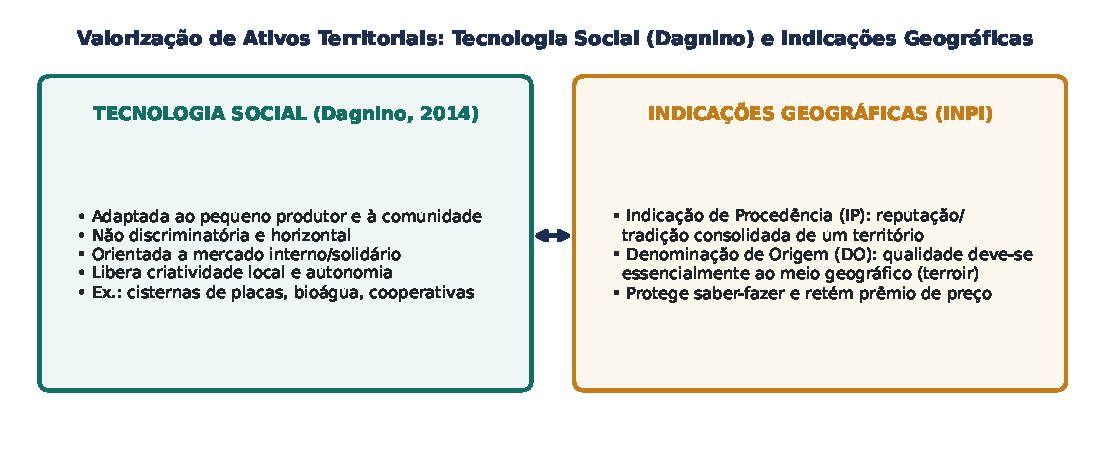
\includegraphics[width=0.94\textwidth]{figures/fig06_tecnologia_social_igs.pdf}
  \caption{Articulação entre Tecnologia Social, Economia Solidária, Bioeconomia e Indicações Geográficas para ampliação da Retenção de Valor Local ($RVL$).}
  \label{fig:tecnologia_social_igs}
\end{figure}

Essa convergência manifesta-se nos territórios baianos, conforme ilustram as subfiguras (a), (b) e (c) da Figura~\ref{fig:igs_tecnologia_bahia}.

\begin{figure}[H]
  \centering
  \begin{minipage}[t]{0.31\textwidth}
    \centering
    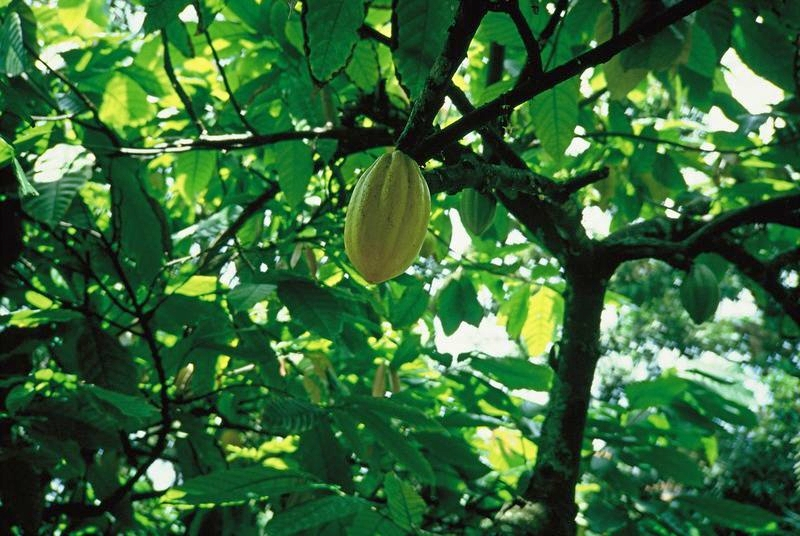
\includegraphics[width=\textwidth,height=3.4cm,keepaspectratio]{figures/foto_cacau_ilheus.jpg}
    \par\small\textbf{(a)} Cacau cultivado no Sul da Bahia (Ilhéus): base para Indicação de Procedência.
  \end{minipage}\hfill
  \begin{minipage}[t]{0.31\textwidth}
    \centering
    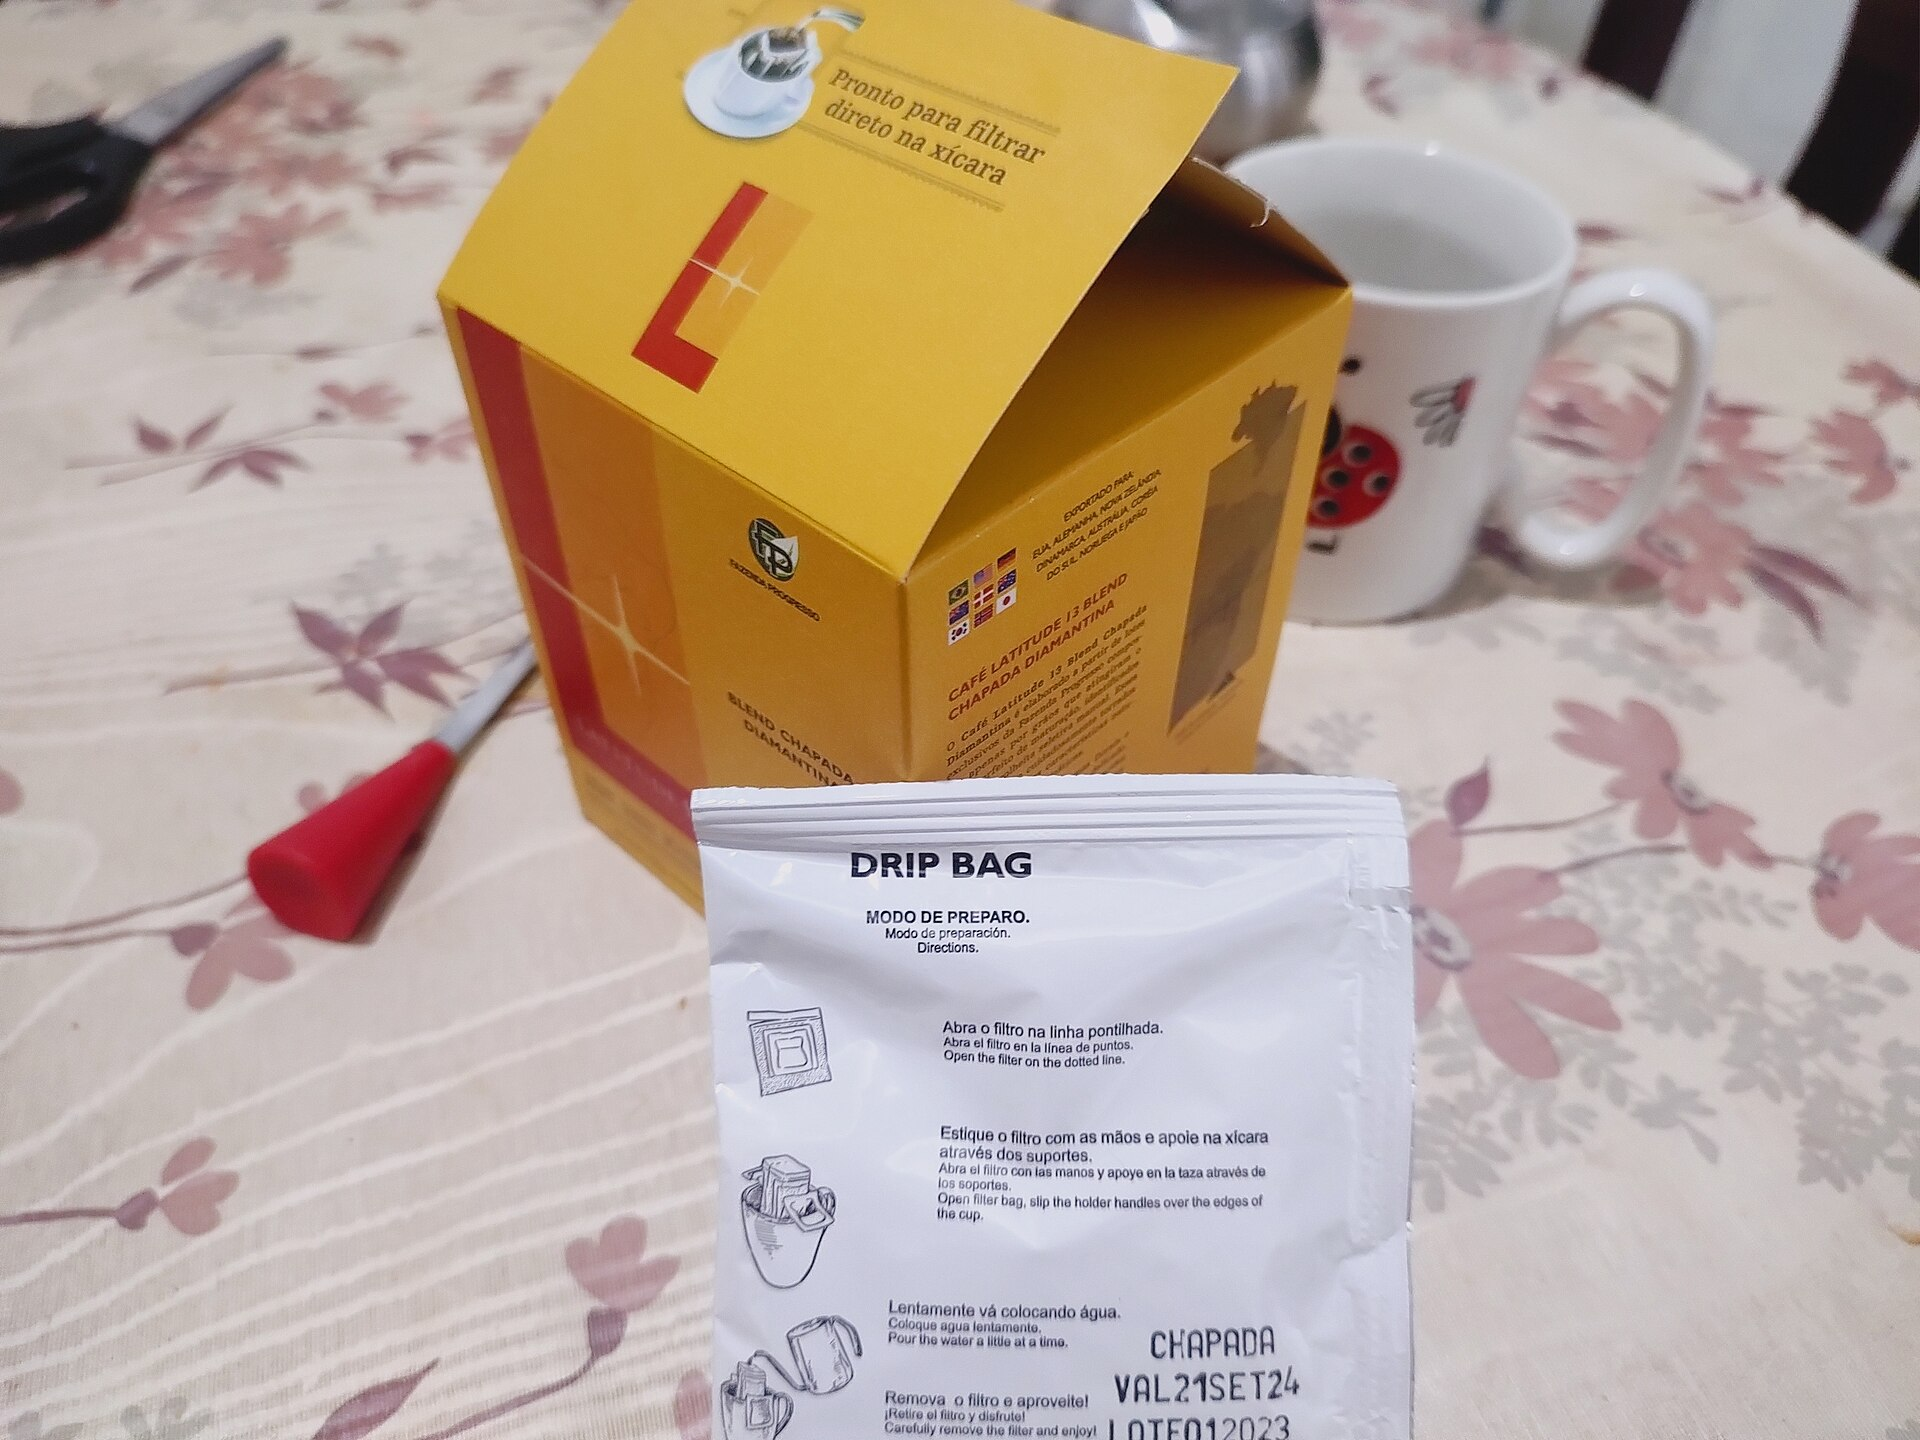
\includegraphics[width=\textwidth,height=3.4cm,keepaspectratio]{figures/foto_cafe_chapada_diamantina.jpg}
    \par\small\textbf{(b)} Café especial de Mucugê na Chapada Diamantina: diferenciação por \textit{terroir}.
  \end{minipage}\hfill
  \begin{minipage}[t]{0.31\textwidth}
    \centering
    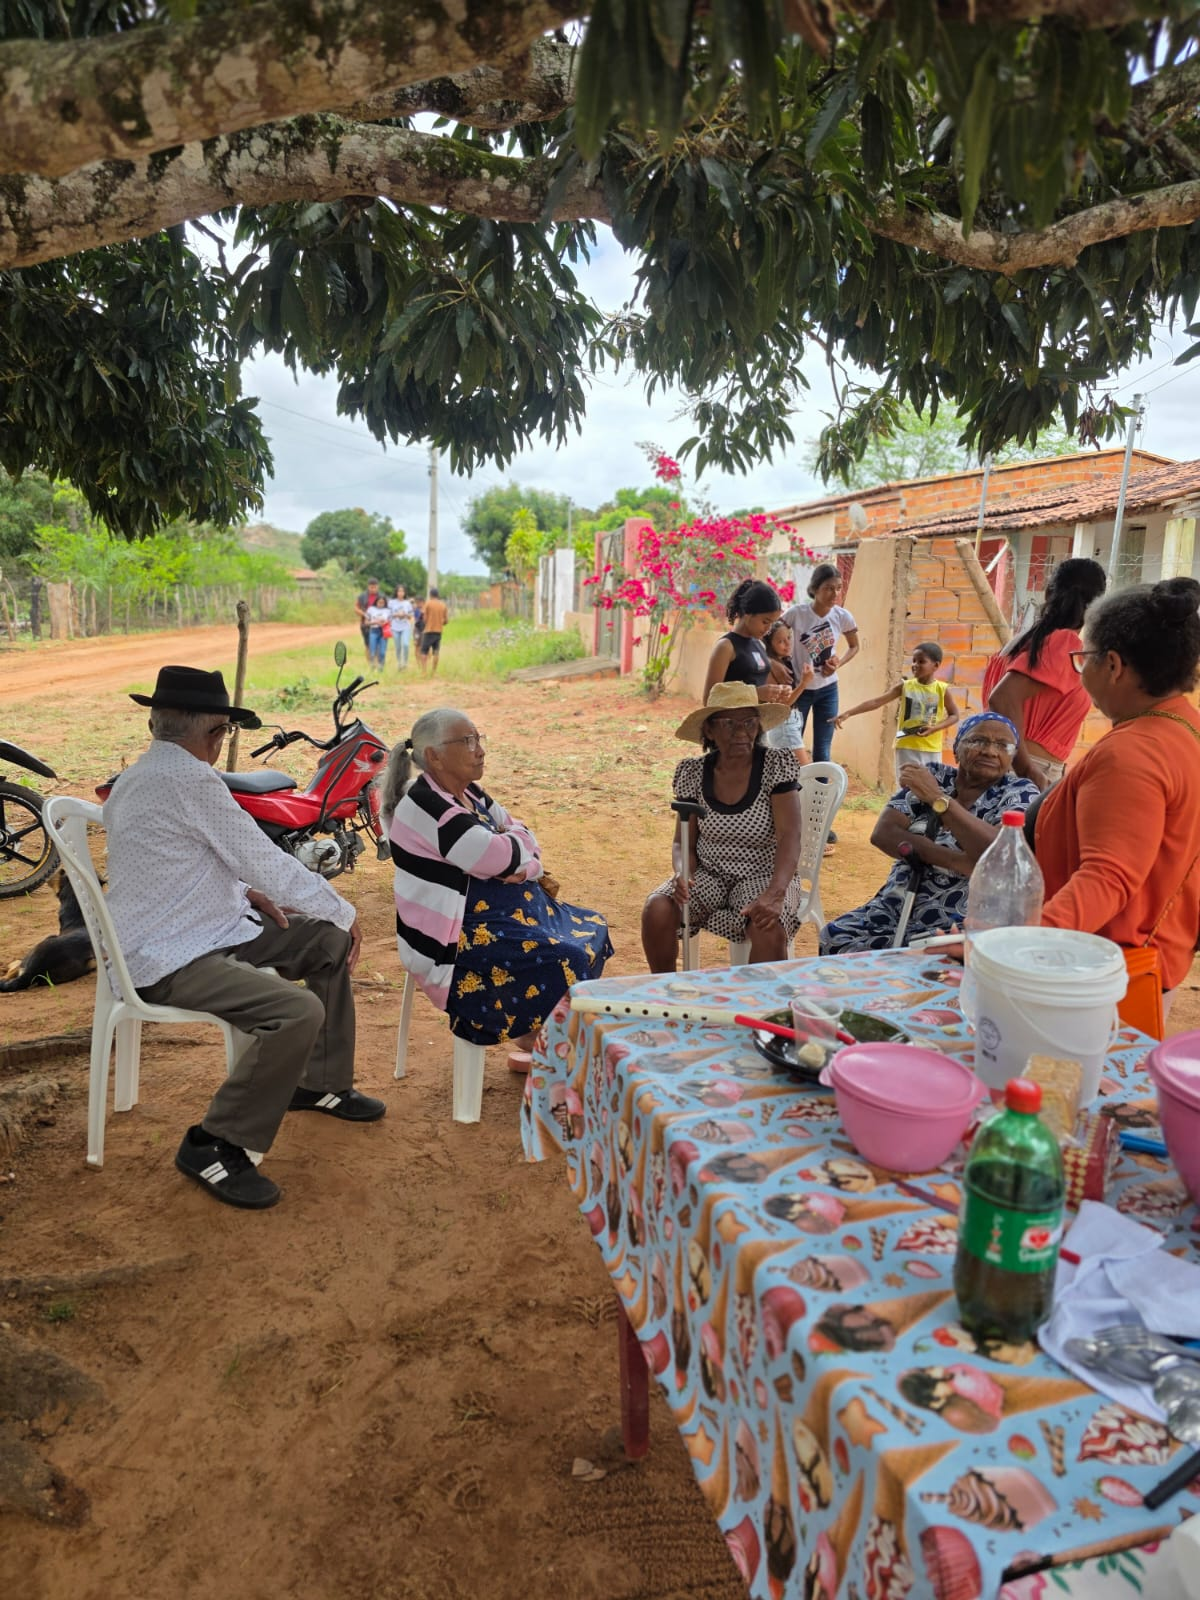
\includegraphics[width=\textwidth,height=3.4cm,keepaspectratio]{figures/foto_quilombo_territorio.jpg}
    \par\small\textbf{(c)} Organização comunitária quilombola em Tranqueira (BA): tecnologia social e território.
  \end{minipage}
  \caption{\textbf{Expressões de diferenciação territorial e tecnologia social na Bahia.} \textit{O que observar:} em (a) e (b), produtos vinculados à origem geográfica substituem a lógica de \textit{commodity} indiferenciada por prêmio de qualidade territorial. Em (c), a organização coletiva em comunidade quilombola exemplifica a retenção de valor apoiada em governança local e saberes tradicionais. Fonte: Wikimedia Commons, CC BY/CC BY-SA (a, b) e Projeto Catuxe/UEFS (c).}
  \label{fig:igs_tecnologia_bahia}
\end{figure}

\begin{boxFormula}[Prêmio de Preço Territorial, Ponto de Equilíbrio e Retenção de Valor Local]
\textbf{1. Prêmio Percentual de Preço Territorial ($\pi_{IG}$):}
\[
\pi_{IG} = \left(\frac{P_{IG} - P_{comm}}{P_{comm}}\right) \times 100\%
\]

\textbf{2. Ganho Líquido Unitário da Certificação ($G_{unit}$) e Volume de Equilíbrio ($Q^*$):}
Considerando o custo anual fixo de governança, rastreabilidade e auditoria da IG ($C_{cert}$) para um volume comercializado $Q$:
\[
G_{unit} = (P_{IG} - P_{comm}) - \frac{C_{cert}}{Q} \qquad \text{e} \qquad Q^* = \frac{C_{cert}}{P_{IG} - P_{comm}}
\]
A IG só gera ganho econômico líquido quando $Q > Q^*$.

\textbf{3. Taxa de Retenção de Valor Local ($RVL$):}
Mede a fração do preço final pago pelo consumidor que efetivamente remunera trabalho, renda e fornecedores dentro do território:
\[
RVL = \left(\frac{V_{remunerado\_local}}{V_{bruto\_final}}\right) \times 100\%
\]
\end{boxFormula}

\subsection{Síntese Integradora para a AV1 (30\%): Seminário e Fichamento Crítico}

A avaliação da Unidade~I (\textbf{AV1, 30\%}) exige que você integre os seis capítulos em um diagnóstico territorial coerente. Um bom fichamento crítico ou seminário deve articular o paradigma tecnológico e o espaço geográfico (Cap.~1) com as barreiras de entrada e a eficiência coletiva (Cap.~2), identificando as lacunas de proximidade e a estrutura do ecossistema local (Cap.~3). A partir dessa base, a análise avança para a governança em hélice e as políticas de CT\&I (Cap.~4), incorpora a arquitetura de impacto e o risco de \textit{mission drift} (Cap.~5) e culmina nas estratégias de adequação sociotécnica, economia solidária e proteção de origem territorial (Cap.~6).

\etapa{4}{Exemplos Resolvidos e Estudos de Caso Comentados}

\begin{boxExemplo}{6.1}{Adequação Sociotécnica no Beneficiamento do Umbu e do Licuri}
\passoEnunciado{Uma cooperativa de mulheres extrativistas no Semiárido recebeu, via doação, uma linha industrial importada de processamento de polpa dimensionada para $10$ toneladas/hora, movida a energia trifásica de alta potência.}
\passoDados{A comunidade produz no máximo $1{,}2$ tonelada/dia na safra sazonal, dispõe de rede elétrica rural monofásica instável e não possui técnicos externos para manutenção de placas eletrônicas proprietárias.}
\passoPedido{Diagnosticar por que a Tecnologia Convencional (TC) falhou no território e propor uma solução de Tecnologia Social (TS) baseada em Adequação Sociotécnica (AST).}
\passoMetodo{Aplicação dos critérios de Adequação Sociotécnica de Renato Dagnino (escala, matriz energética, autonomia de manutenção e controle coletivo).}
\passoContas{
1. Diagnóstico da TC: superdimensionamento ($10\text{ t/h}$ vs. oferta de $1{,}2\text{ t/dia}$ gera ociosidade superior a $95\%$ e custo fixo impagável); incompatibilidade elétrica; caixa-preta tecnológica dependente de peças importadas.\\
2. Redesenho via AST: adoção de despolpadeiras modulares de aço inox em pequena escala ($150\text{ kg/h}$ cada), alimentadas por sistema solar fotovoltaico descentralizado e com mecânica aberta passível de manutenção por serralheiros e eletricistas do próprio município.
}
\passoResposta{A TC geraria endividamento e paralisação; a TS via módulos solares descentralizados ajusta escala, energia e autonomia técnica à realidade da cooperativa.}
\passoVerificacao{O exemplo ilustra que eficiência técnica abstrata (litros ou toneladas por hora) não equivale à eficiência econômica e territorial.}
\end{boxExemplo}

\begin{boxExemplo}{6.2}{Distribuição de Sobras em Cooperativa Solidária Autogestionária}
\passoEnunciado{Uma cooperativa agroextrativista solidária encerrou o exercício anual e precisa deliberar em assembleia sobre a destinação de suas sobras líquidas.}
\passoDados{Receita bruta anual: $\reais{480.000,00}$. Custos operacionais e despesas administrativas totais: $\reais{330.000,00}$. O estatuto prevê destinação de $10\%$ da sobra bruta para o Fundo de Reserva e $5\%$ para o FATES (assistência técnica e educação cooperativista). O total de horas trabalhadas pelo conjunto dos cooperados no ano foi de $42.500\text{ h}$.}
\passoPedido{Calcular a sobra bruta, os valores retidos nos fundos coletivos, a sobra distribuível e o rateio correspondente a uma cooperada que trabalhou $1.800\text{ h}$ no ano.}
\passoMetodo{Apuração contábil cooperativista (Lei n.\textsuperscript{o} 5.764/1971) e rateio proporcional ao trabalho.}
\passoContas{
1. Sobra bruta: $S_{bruta} = 480.000 - 330.000 = \reais{150.000,00}$.\\
2. Retenções estatutárias: Fundo de Reserva ($10\%$) $= \reais{15.000,00}$; FATES ($5\%$) $= \reais{7.500,00}$. Total retido $= \reais{22.500,00}$.\\
3. Sobra distribuível:
\[
S_{dist} = 150.000 - 22.500 = \reais{127.500,00}
\]
4. Valor por hora trabalhada e cota da cooperada ($1.800\text{ h}$):
\[
v_h = \frac{127.500}{42.500} = \reais{3,00}/\text{hora} \implies \text{Cota} = 1.800 \times 3{,}00 = \reais{5.400,00}
\]
}
\passoResposta{A sobra distribuível é de $\reais{127.500,00}$ ($\reais{3,00}/\text{hora}$), cabendo $\reais{5.400,00}$ à cooperada, além de $\reais{22.500,00}$ reinvestidos na resiliência e formação coletiva.}
\passoVerificacao{Diferentemente de sociedades anônimas que remuneram o capital investido, a cooperativa remunera o trabalho efetivo e fortalece reservas indivisíveis do território.}
\end{boxExemplo}

\begin{boxExemplo}{6.3}{Prêmio de Preço Territorial e Ponto de Equilíbrio no Cacau do Sul da Bahia}
\passoEnunciado{Uma associação de produtores agroflorestais avalia aderir ao selo de Indicação de Procedência (IP) do Cacau do Sul da Bahia para comercializar amêndoas fermentadas finas.}
\passoDados{Preço de referência do cacau \textit{commodity}: $P_{comm} = \reais{18,00}/\text{kg}$. Preço alcançado com o selo IP e rastreabilidade: $P_{IG} = \reais{27,00}/\text{kg}$. Custo anual fixo de auditoria, selos e governança da associação para esse grupo: $C_{cert} = \reais{36.000,00}/\text{ano}$. Produção anual comercializada pelo grupo: $Q = 12.000\text{ kg/ano}$.}
\passoPedido{Calcular o prêmio percentual de preço ($\pi_{IG}$), o ganho líquido unitário ($G_{unit}$) e o volume mínimo de equilíbrio ($Q^*$).}
\passoMetodo{Aplicação das equações de prêmio territorial e ponto de equilíbrio de certificação.}
\passoContas{
1. Prêmio percentual de preço:
\[
\pi_{IG} = \left(\frac{27{,}00 - 18{,}00}{18{,}00}\right) \times 100\% = \frac{9{,}00}{18{,}00} \times 100\% = 50{,}0\%
\]
2. Custo de certificação por quilograma e ganho líquido unitário:
\[
\frac{C_{cert}}{Q} = \frac{36.000}{12.000} = \reais{3,00}/\text{kg} \implies G_{unit} = (27{,}00 - 18{,}00) - 3{,}00 = \reais{6,00}/\text{kg}
\]
3. Volume mínimo de equilíbrio ($Q^*$):
\[
Q^* = \frac{36.000}{27{,}00 - 18{,}00} = \frac{36.000}{9{,}00} = 4.000\text{ kg/ano}
\]
}
\passoResposta{O prêmio de preço é de $50{,}0\%$, gerando ganho líquido de $\reais{6,00}/\text{kg}$ ($\reais{72.000,00}/\text{ano}$ adicionais). O grupo opera bem acima do ponto de equilíbrio de $4.000\text{ kg/ano}$.}
\passoVerificacao{O resultado explica por que pequenos produtores individuais não conseguem arcar sozinhos com custos fixos de certificação ($C_{cert}$): a governança coletiva é condição econômica para diluir o custo fixo.}
\end{boxExemplo}

\begin{boxExemplo}{6.4}{Retenção de Valor Local ($RVL$) no Café da Chapada Diamantina}
\passoEnunciado{Compare duas estratégias de inserção comercial para o café especial produzido por uma cooperativa da Chapada Diamantina: venda como grão verde \textit{commodity} para exportadoras externas versus torrefação e embalagem própria com selo de Indicação Geográfica.}
\passoDados{Preço final médio pago pelo consumidor no varejo nacional: $V_{bruto\_final} = \reais{60,00}/\text{kg}$.\\
\textbf{Cenário A (grão verde sem marca territorial):} cooperativa vende o quilo a $\reais{22,00}$ para intermediário externo; insumos químicos externos consumidos na lavoura somam $\reais{10,00}/\text{kg}$.\\
\textbf{Cenário B (café torrado, embalado e certificado com IG local):} cooperativa vende diretamente ou via varejo parceiro retendo $\reais{54,00}/\text{kg}$ no território; insumos e embalagens adquiridos de fora do território somam $\reais{14,00}/\text{kg}$.}
\passoPedido{Calcular o valor líquido retido no território por quilograma e a Taxa de Retenção de Valor Local ($RVL$) em ambos os cenários.}
\passoMetodo{Cálculo de $V_{remunerado\_local} = \text{Receita local} - \text{Insumos externos}$ e razão $RVL = (V_{remunerado\_local}/V_{bruto\_final}) \times 100\%$.}
\passoContas{
\textbf{Cenário A (\textit{commodity}):}
\[
V_{local, A} = 22{,}00 - 10{,}00 = \reais{12,00}/\text{kg} \implies RVL_A = \left(\frac{12{,}00}{60{,}00}\right) \times 100\% = 20{,}0\%
\]
\textbf{Cenário B (agroindustrialização territorial + IG):}
\[
V_{local, B} = 54{,}00 - 14{,}00 = \reais{40,00}/\text{kg} \implies RVL_B = \left(\frac{40{,}00}{60{,}00}\right) \times 100\% \approx 66{,}7\%
\]
}
\passoResposta{A transição para torrefação local com IG eleva a retenção de valor de $\reais{12,00}/\text{kg}$ ($RVL = 20{,}0\%$) para $\reais{40,00}/\text{kg}$ ($RVL = 66{,}7\%$), mais que triplicando a renda retida no território.}
\passoVerificacao{O cálculo materializa a epígrafe da apostila: internalizar etapas industriais e proteger a origem impede o vazamento de valor agregado para fora da região.}
\end{boxExemplo}

\begin{boxExemplo}{6.5}{Roteiro Integrador da AV1: Caso da Cachaça de Abaíra}
\passoEnunciado{Para o Seminário da AV1, um grupo analisa a Indicação de Procedência da Cachaça da Microrregião de Abaíra (BA).}
\passoDados{Produção artesanal em alambiques de cobre por pequenos produtores, organizada via associação local (APAMA), com tradição histórica na Chapada Diamantina e desafios de sucessão geracional e tratamento de vinhoto.}
\passoPedido{Integrar os conceitos da Unidade~I (Caps.~2, 4 e 6) para estruturar um diagnóstico territorial sintético da cadeia.}
\passoMetodo{Síntese cruzada de barreiras de entrada (Cap.~2), Hélice Quíntupla (Cap.~4) e IG/Tecnologia Social (Cap.~6).}
\passoContas{
\begin{enumerate}[leftmargin=1.4em, itemsep=2pt]
  \item \textbf{Barreiras e Eficiência Coletiva (Cap.~2):} a IP cria uma barreira de entrada por diferenciação territorial impossível de ser copiada por destilarias industriais de grande escala; a associação dilui custos de engarrafamento e controle de qualidade.
  \item \textbf{Hélice Quíntupla (Cap.~4):} integração entre produtores, universidades/IFs (padronização fermentativa e aproveitamento do vinhoto para fertirrigação/biogás, Hélice 5), governo (FAPs e extensão rural) e turismo cultural local (Hélice 4).
  \item \textbf{Tecnologia Social e IG (Cap.~6):} preservação do saber-fazer artesanal com adequação sociotécnica sanitária, evitando descaracterização industrial.
\end{enumerate}
}
\passoResposta{O diagnóstico integra diferenciação de mercado, governança participativa e proteção jurídica coletiva do \textit{terroir}, atendendo integralmente à rubrica analítica da AV1.}
\passoVerificacao{A articulação entre capítulos transforma conceitos isolados em estratégia prática de desenvolvimento territorial.}
\end{boxExemplo}

\etapa{5}{Armadilhas Conceituais e Erros Mais Comuns}

\begin{boxErro}[Erro 1: Confundir Indicação de Procedência (IP) com Denominação de Origem (DO)]
Embora ambas sejam Indicações Geográficas registradas no INPI, a \textbf{IP} baseia-se na \textit{notoriedade} da região como centro produtor, enquanto a \textbf{DO} exige comprovação técnico-científica de que as características do produto decorrem essencial ou exclusivamente do meio geográfico (fatores naturais + humanos).
\end{boxErro}

\begin{boxErro}[Erro 2: Tratar a Indicação Geográfica como Marca Privada]
Uma marca comercial pertence a uma empresa específica e pode ser vendida ou licenciada a qualquer fábrica fora da região. A IG é um \textbf{direito coletivo de uso} vinculado ao território delimitado e ao cumprimento do caderno de especificações técnicas; ninguém de fora da área demarcada pode utilizá-la.
\end{boxErro}

\begin{boxErro}[Erro 3: Reduzir Tecnologia Social a ``Tecnologia Pobre ou Improvisada'']
Tecnologia Social não significa gambiarra de baixa qualidade. Exige rigor científico e engenharia aplicada para construir soluções eficientes em pequena escala, com baixo impacto ambiental e controle pelos trabalhadores locais.
\end{boxErro}

\begin{boxErro}[Erro 4: Achar que o Selo de IG Vende Sozinho Sem Governança]
Obter o registro no INPI é apenas o ponto de partida. Sem rastreabilidade efetiva, controle de qualidade contínuo e estratégia comercial coletiva, o selo não gera prêmio de preço ($\pi_{IG} = 0$) e o custo de certificação ($C_{cert}$) torna-se um passivo para os produtores.
\end{boxErro}

\etapa{6}{Exercícios Propostos (Básicos, Intermediários e Objetivos)}

\textbf{Parte A, Exercícios Básicos (Conceituação e Identificação)}

\textbf{1.} Explique a tese de Renato Dagnino sobre a não neutralidade da Tecnologia Convencional (TC) e defina Adequação Sociotécnica (AST).
\espacoResolucao[1.8cm]

\textbf{2.} Qual é a diferença fundamental entre o destino do excedente em uma empresa capitalista tradicional e em uma cooperativa de economia solidária?
\espacoResolucao[1.8cm]

\textbf{3.} Diferencie Indicação de Procedência (IP) de Denominação de Origem (DO) segundo a Lei n.\textsuperscript{o} 9.279/1996.
\espacoResolucao[1.8cm]

\textbf{4.} Cite dois exemplos de produtos baianos com Indicação Geográfica reconhecida (ou em consolidação) e descreva o ativo territorial protegido em cada um.
\espacoResolucao[1.8cm]

\textbf{5.} Por que a bioeconomia territorial se opõe ao modelo de extrativismo primário exportador?
\espacoResolucao[1.8cm]

\textbf{Parte B, Exercícios Intermediários (Modelagem e Análise Quantitativa)}

\textbf{6.} Uma associação de apicultores vende mel comum a $P_{comm} = \reais{20,00}/\text{kg}$. Após conquistar o registro de IG, passa a vender a $P_{IG} = \reais{31,00}/\text{kg}$. O custo fixo anual de auditoria e selos é $C_{cert} = \reais{22.000,00}$ para uma produção anual de $Q = 5.000\text{ kg}$. Calcule $\pi_{IG}$, $G_{unit}$ e $Q^*$.
\espacoResolucao[2.0cm]

\textbf{7.} Um queijo artesanal certificado é vendido no varejo a $V_{bruto\_final} = \reais{80,00}/\text{kg}$. Na venda direta via cooperativa territorial, os produtores retêm $\reais{52,00}/\text{kg}$ líquidos após descontar embalagens e fermentos comprados fora da região. Calcule a Taxa de Retenção de Valor Local ($RVL$).
\espacoResolucao[2.0cm]

\textbf{8.} Uma cooperativa solidária obteve sobra bruta de $\reais{100.000,00}$, destinou $10\%$ ao Fundo de Reserva e $10\%$ ao FATES. Com $20.000$ horas trabalhadas pelos sócios no ano, quanto receberá um cooperado que acumulou $1.500$ horas?
\espacoResolucao[2.0cm]

\textbf{9.} Um projeto de implantação de biodigestores rurais fracassou em um assentamento porque exigia peças importadas e manutenção de empresa sediada a $600\text{ km}$. Proponha três ajustes de Adequação Sociotécnica para viabilizar o projeto.
\espacoResolucao[2.0cm]

\textbf{10.} Estruture um roteiro de 4 etapas para o Fichamento Crítico da AV1 integrando um território de sua escolha aos conceitos de Tecnopolos/Habitats (Cap.~4), Impacto (Cap.~5) e IGs/TS (Cap.~6).
\espacoResolucao[2.0cm]

\textbf{Parte C, Questões Objetivas (Estilo Exame / Concurso, A a E)}

\textbf{11.} Segundo Renato Dagnino (2014), a Tecnologia Convencional frequentemente entra em conflito com empreendimentos de economia solidária porque:
\begin{alternativas}
  \item É gratuita e de código aberto, impedindo a proteção por patentes.
  \item Incorpora valores da grande empresa capitalista, como economia de mão de obra, alta escala e controle hierárquico, incompatíveis com a autogestão.
  \item Exige obrigatoriamente que todos os trabalhadores tenham título de doutorado.
  \item Não pode ser aplicada em ambientes urbanos industriais.
  \item Elimina a necessidade de energia elétrica ou insumos externos.
\end{alternativas}

\textbf{12.} De acordo com a Lei n.\textsuperscript{o} 9.279/1996 (Lei da Propriedade Industrial), a modalidade de Indicação Geográfica que exige comprovação de que as qualidades do produto decorrem exclusiva ou essencialmente do meio geográfico (fatores naturais e humanos) é denominada:
\begin{alternativas}
  \item Patente de Modelo de Utilidade.
  \item Marca de Alto Renome.
  \item Indicação de Procedência (IP).
  \item Denominação de Origem (DO).
  \item Desenho Industrial Coletivo.
\end{alternativas}

\textbf{13.} Uma cooperativa de derivados de mandioca comercializa farinha especial com IG a $\reais{15,00}/\text{kg}$, frente ao preço de $\reais{10,00}/\text{kg}$ da farinha comum. Sabendo que o custo fixo anual de certificação é de $\reais{25.000,00}$, o volume mínimo de equilíbrio ($Q^*$) para que a certificação comece a gerar ganho líquido positivo é de:
\begin{alternativas}
  \item $1.667\text{ kg/ano}$
  \item $2.500\text{ kg/ano}$
  \item $5.000\text{ kg/ano}$
  \item $7.500\text{ kg/ano}$
  \item $10.000\text{ kg/ano}$
\end{alternativas}

\textbf{14.} Sobre os princípios da Economia Solidária e da autogestão, assinale a alternativa \textbf{correta}:
\begin{alternativas}
  \item O poder de voto nas assembleias é proporcional ao capital integralizado por cada sócio.
  \item As sobras distribuíveis são partilhadas conforme critérios definidos coletivamente (como trabalho ou produção entregue), após constituição dos fundos legais.
  \item A propriedade dos equipamentos pertence a um investidor-anjo externo sem vínculo com o trabalho local.
  \item É vedada a formação de redes de cooperação entre empreendimentos solidários.
  \item Os empreendimentos solidários não podem atuar em cadeias da bioeconomia.
\end{alternativas}

\textbf{15.} Em cadeias produtivas da sociobiodiversidade, a elevação da Taxa de Retenção de Valor Local ($RVL$) ocorre principalmente quando o território:
\begin{alternativas}
  \item Exporta matéria-prima bruta sem beneficiamento e importa produtos acabados.
  \item Substitui espécies nativas por monoculturas dependentes de pacotes químicos externos.
  \item Internaliza etapas de beneficiamento, rastreabilidade e diferenciação por origem (como IGs), reduzindo a dependência de intermediários externos.
  \item Elimina cooperativas para concentrar a terra em um único comprador monopsônico.
  \item Adota pacotes tecnológicos convencionais sem adequação sociotécnica.
\end{alternativas}

\etapa{7}{Questões Autorais Estilo Pós-Graduação e Concursos}

\textbf{16. (Estilo Concurso para Analista de Propriedade Industrial, INPI)} Uma associação de produtores de mel de uma região semiárida deseja registrar uma Indicação Geográfica. A região já possui notoriedade histórica pela produção apícola há 40 anos, mas ainda não dispõe de estudos laboratoriais completos que comprovem a correlação exclusiva entre a flora nativa local e parâmetros físico-químicos específicos do mel. Oriente a associação sobre qual modalidade (IP ou DO) deve ser pleiteada inicialmente e quais evidências técnicas e documentais são exigidas.
\espacoResolucao[2.2cm]

\textbf{17. (Estilo Pós-Graduação em Desenvolvimento Territorial)} Analise o paradoxo da ``mercantilização sem retenção'': em diversas regiões, produtos tradicionais conquistam selos de qualidade e prêmios internacionais, mas a maior parte do valor adicionado continua apropriada por torrefadoras, distribuidoras ou marcas sediadas em metrópoles externas. Proponha estratégias combinadas de Tecnologia Social, Economia Solidária e governança de IG para reverter esse vazamento de valor.
\espacoResolucao[2.2cm]

\textbf{18. (Estilo Mestrado Profissional, PLANTERR/UEFS)} Escolha um arranjo produtivo da sociobiodiversidade baiana (ex.: licuri, umbu, piaçava, cacau cabruca ou cachaça artesanal) e redija um plano sintético articulando: (a) um processo de Adequação Sociotécnica; (b) um modelo de governança autogestionária ou híbrida sem \textit{mission drift}; e (c) estimativa conceitual de como a IG eleva o prêmio de preço ($\pi_{IG}$) e a $RVL$.
\espacoResolucao[2.2cm]

\begin{boxDica}[Checklist Final para a Entrega da AV1 (30\%)]
Antes de apresentar seu Seminário ou entregar o Fichamento Crítico da \textbf{AV1}, verifique se sua análise responde a três perguntas-chave da Unidade~I:
\begin{enumerate}[leftmargin=1.4em, itemsep=2pt]
  \item \textbf{Tecnologia e Território:} a solução proposta é compatível com a escala, a cultura e os recursos locais (AST)?
  \item \textbf{Governança:} as cinco hélices estão articuladas sem captura por interesses privados (socialização do risco)?
  \item \textbf{Retenção de Valor:} o modelo amplia a $RVL$ e protege o patrimônio coletivo territorial?
\end{enumerate}
\end{boxDica}

\clearpage
\etapa{8}{Gabarito Comentado dos 18 Exercícios}

\begin{boxGabarito}[Respostas Comentadas: Capítulo 6]
\textbf{1.} Para Dagnino, a TC embute relações sociais capitalistas (alta escala, substituição de trabalho, dependência de insumos externos), não sendo neutra. A AST consiste no processo participativo de adaptar ou redesenhar tecnologias para que se tornem compatíveis com o controle coletivo e a realidade local.

\textbf{2.} Na empresa capitalista, o lucro remunera o capital investido pelos acionistas; na cooperativa solidária, as sobras (após fundos coletivos) retornam proporcionalmente ao trabalho ou à produção entregue pelos cooperados.

\textbf{3.} A Indicação de Procedência (IP) protege a notoriedade/reputação geográfica do local como centro produtor; a Denominação de Origem (DO) exige nexo causal comprovado de que as qualidades do produto devem-se essencial ou exclusivamente ao meio geográfico (fatores naturais e humanos).

\textbf{4.} Cacau do Sul da Bahia (IP, protege a tradição do sistema cabruca e a qualidade das amêndoas) e Cachaça de Abaíra (IP, protege o saber-fazer artesanal da microrregião na Chapada Diamantina).

\textbf{5.} Porque busca internalizar etapas de processamento, conhecimento científico, rastreabilidade e agregação de valor no território de origem, conservando a sociobiodiversidade em pé em vez de exportar matéria-prima bruta a baixo preço.

\textbf{6.} $\pi_{IG} = [(31 - 20)/20] \times 100\% = 55{,}0\%$. Custo unitário de certificação $= 22.000 / 5.000 = \reais{4,40}/\text{kg}$. $G_{unit} = (31 - 20) - 4{,}40 = \reais{6,60}/\text{kg}$. $Q^* = 22.000 / (31 - 20) = 2.000\text{ kg/ano}$.

\textbf{7.} $RVL = (52{,}00 / 80{,}00) \times 100\% = 65{,}0\%$.

\textbf{8.} Retenção total $= 20\%$ ($\reais{20.000,00}$). Sobra distribuível $= \reais{80.000,00}$. Valor por hora $= 80.000 / 20.000 = \reais{4,00}/\text{h}$. Cota do cooperado $= 1.500 \times 4{,}00 = \reais{6.000,00}$.

\textbf{9.} (i) Substituir peças proprietárias por componentes padronizados disponíveis no comércio regional; (ii) capacitar jovens e moradores locais como técnicos de manutenção; (iii) adaptar a capacidade dos biodigestores ao volume real de biomassa de cada unidade familiar.

\textbf{10.} Roteiro sugerido: (1) caracterização produtiva e barreiras do território; (2) mapeamento da Hélice Quíntupla e instrumentos de CT\&I aplicáveis; (3) avaliação de impacto via Teoria da Mudança e risco de \textit{mission drift}; (4) estratégia de AST, autogestão e proteção via IG para maximizar a $RVL$.

\textbf{11. (B)} Dagnino demonstra que a TC não é neutra, pois incorpora objetivos de acumulação e controle hierárquico incompatíveis com a autogestão solidária.

\textbf{12. (D)} A Denominação de Origem (art. 178 da Lei n.\textsuperscript{o} 9.279/1996) exige nexo causal entre as características do produto e o meio geográfico (fatores naturais e humanos).

\textbf{13. (C)} $Q^* = 25.000 / (15 - 10) = 25.000 / 5 = 5.000\text{ kg/ano}$.

\textbf{14. (B)} Na autogestão cooperativista, cada sócio tem um voto (independentemente do capital) e as sobras distribuíveis remuneram o trabalho ou a produção entregue.

\textbf{15. (C)} A retenção de valor local aumenta quando o território internaliza processamento, governança e diferenciação de origem.

\textbf{16.} Deve pleitear inicialmente a \textbf{Indicação de Procedência (IP)}, pois já dispõe de notoriedade histórica de 40 anos como centro produtor. Exigirá: delimitação da área geográfica, regulamento de uso/caderno de especificações técnicas, comprovação documental da reputação (reportagens, registros históricos, feiras) e estrutura de controle pela associação representativa. Futuramente, com estudos polínicos e físico-químicos que comprovem o nexo com o \textit{terroir}, poderá evoluir para DO.

\textbf{17.} Para evitar que o selo apenas valorize o produto nas mãos de terceiros externos, deve-se: (i) exigir no caderno de especificações que etapas críticas de beneficiamento/embalagem ocorram dentro da área demarcada; (ii) constituir agroindústrias cooperativas autogestionárias com tecnologias sociais modulares; (iii) estruturar comercialização direta em redes solidárias e compras públicas territoriais.

\textbf{18.} Resposta aberta integrando o arranjo escolhido: deve detalhar o redesenho sociotécnico de equipamentos (AST), a proteção contra captura por atravessadores (governança cooperativa) e o mecanismo pelo qual o selo de origem converte commodity regional em produto diferenciado com maior $RVL$.
\end{boxGabarito}

\begin{boxResumo}
\begin{itemize}[leftmargin=1.4em, itemsep=3pt]
  \item A \textbf{Tecnologia Social} e a \textbf{Adequação Sociotécnica} (Dagnino) adaptam soluções produtivas à escala, cultura e autonomia dos trabalhadores do território.
  \item A \textbf{Economia Solidária} baseia-se na autogestão e na partilha de sobras proporcionais ao trabalho/produção, fortalecendo reservas coletivas.
  \item As \textbf{Indicações Geográficas} (IP por notoriedade; DO por nexo causal com o \textit{terroir}) são ativos coletivos que geram prêmio de preço ($\pi_{IG}$) e ampliam a \textbf{Retenção de Valor Local ($RVL$)}, desde que o volume supere o ponto de equilíbrio $Q^*$.
\end{itemize}
\end{boxResumo}

\begin{boxTeste}
Julgue os itens a seguir como Verdadeiros (\V) ou Falsos (\F):
\begin{enumerate}[leftmargin=1.6em, itemsep=3pt]
  \item (\quad) A Adequação Sociotécnica defende que toda tecnologia industrial de grande escala deve ser implantada sem alterações em cooperativas rurais.
  \item (\quad) Na Denominação de Origem (DO), exige-se comprovação de que as qualidades do produto decorrem exclusiva ou essencialmente do meio geográfico, incluindo fatores naturais e humanos.
  \item (\quad) Quando o volume comercializado $Q$ é inferior ao ponto de equilíbrio $Q^* = C_{cert}/(P_{IG} - P_{comm})$, o custo fixo de certificação supera o ganho adicional de preço da IG.
  \item (\quad) A internalização de etapas de beneficiamento e embalagem no território reduz a Taxa de Retenção de Valor Local ($RVL$).
\end{enumerate}
\textbf{Gabarito do Checkpoint:} 1. \F \quad 2. \V \quad 3. \V \quad 4. \F \text{ (eleva a } RVL\text{)}
\end{boxTeste}

\clearpage
\phantomsection
\addcontentsline{toc}{chapter}{Simulado I: Revisão Integrada da Unidade I (AV1)}
\chapter*{Simulado e Revisão Integrada da Unidade I (Preparatório AV1: 30\%)}
\markboth{SIMULADO, UNIDADE I}{SIMULADO, UNIDADE I}

\begin{capObjetivos}
Este simulado integra os conteúdos dos \textbf{Capítulos 1 a 6} (\textbf{Unidade I, Território e Ecossistemas}), servindo como preparação direta para o Seminário e Fichamento Crítico da \textbf{AV1 (30\%)}. Resolva as \textbf{8 questões objetivas (A--E)} e as \textbf{2 questões dissertativas críticas} antes de consultar o gabarito comentado, o espelho dissertativo e a tabela de diagnóstico.
\end{capObjetivos}

\etapa{1}{Questões Objetivas Integradas (Capítulos 1 a 6)}

\textbf{Questão 1 (Cap. 1, Schumpeter, Dosi e Espaço Territorial)}
Considerando a articulação entre inovação tecnológica e desenvolvimento territorial (Schumpeter, Kuhn, Dosi e Milton Santos), assinale a alternativa \textbf{correta}:
\begin{alternativas}
  \item A destruição criadora schumpeteriana distribui seus benefícios de modo uniforme por todo o espaço geográfico, independentemente da densidade técnica local.
  \item Paradigmas e trajetórias tecnológicas (Dosi) orientam a busca por soluções técnicas e tendem a se concentrar em territórios com maior densidade de infraestrutura, conhecimento e normas (meio técnico-científico-informacional).
  \item A inovação incremental corresponde a rupturas radicais de paradigma científico que inviabilizam todas as firmas incumbentes de imediato.
  \item Na leitura de Milton Santos, o território é apenas um suporte físico passivo, sem influência sobre a apropriação do valor tecnológico.
  \item O empreendedorismo de base tecnológica independe de trajetórias tecnológicas prévias ou de instituições regionais de ensino e pesquisa.
\end{alternativas}

\textbf{Questão 2 (Cap. 2, Estruturas de Mercado e Eficiência Coletiva)}
Em um Arranjo Produtivo Local (APL) de confecções ou calçados formado por microempresas, a superação de desvantagens de escala diante de grandes concorrentes externos ocorre principalmente por meio da \textbf{eficiência coletiva}, que combina:
\begin{alternativas}
  \item Monopólio legal concedido pelo município e eliminação de fornecedores especializados locais.
  \item Externalidades passivas da aglomeração (como concentração de mão de obra e fornecedores) somadas a ações conjuntas deliberadas (compras coletivas, consórcios de exportação e laboratórios compartilhados).
  \item Guerra fiscal predatória entre as próprias empresas do arranjo para reduzir salários abaixo do mínimo legal.
  \item Integração vertical absoluta de cada microempresa, proibindo a subcontratação local.
  \item Substituição integral da cooperação territorial pela importação de produtos acabados.
\end{alternativas}

\textbf{Questão 3 (Cap. 3, Ecossistemas Empreendedores e Proximidades de Boschma)}
Segundo Ron Boschma, a proximidade geográfica entre empresas e universidades \textbf{não garante} por si só o aprendizado inovativo, pois a cooperação eficaz exige equilíbrio entre outras dimensões de proximidade. O risco de \textit{lock-in} (aprisionamento cognitivo e rotinas obsoletas) em um território ocorre tipicamente quando há:
\begin{alternativas}
  \item Excesso de proximidade cognitiva, organizacional e institucional, reduzindo a entrada de novas ideias e o questionamento de práticas antigas.
  \item Baixa distância geográfica combinada com alta diversidade de atores em Hélice Quíntupla.
  \item Existência de intermediários tecnológicos (NITs) conectando a região a redes internacionais de pesquisa.
  \item Presença simultânea de \textit{startups}, cooperativas e fundos de fomento público.
  \item Renovação periódica das trajetórias tecnológicas por meio de políticas orientadas por missões.
\end{alternativas}

\textbf{Questão 4 (Cap. 4, Governança em Hélice Quíntupla e Marco Legal de CT\&I)}
Uma empresa tributada pelo \textbf{Lucro Real} investiu $\reais{1.500.000,00}$ em P\&D elegível e obteve direito à exclusão adicional de $\alpha_{excl} = 80\%$ pela Lei do Bem (Lei n.\textsuperscript{o} 11.196/2005). Considerando alíquota efetiva combinada de IRPJ e CSLL de $34\%$, a economia fiscal incentivada ($E_{LeiBem}$) e o instrumento adequado caso um órgão público queira contratar o desenvolvimento de uma solução com risco tecnológico ainda não disponível no mercado são, respectivamente:
\begin{alternativas}
  \item $\reais{306.000,00}$ e Pregão Eletrônico por Menor Preço.
  \item $\reais{408.000,00}$ e Encomenda Tecnológica (ETEC, Lei n.\textsuperscript{o} 13.243/2016).
  \item $\reais{510.000,00}$ e Parceria Público-Privada de Concessão Rodoviária.
  \item $\reais{408.000,00}$ e Isenção do Simples Nacional.
  \item $\reais{612.000,00}$ e Encomenda Tecnológica (ETEC, Lei n.\textsuperscript{o} 13.243/2016).
\end{alternativas}

\textbf{Questão 5 (Cap. 4, Estado Empreendedor e Habitats de Inovação)}
Na análise crítica de políticas de CT\&I, a expressão ``catedral no deserto'' e a crítica de Mariana Mazzucato à ``socialização do risco com privatização dos ganhos'' referem-se, respectivamente, a:
\begin{alternativas}
  \item Parques tecnológicos integrados às cadeias locais e cobrança de \textit{royalties} públicos sobre patentes financiadas pelo Estado.
  \item Infraestrutura física de inovação desconectada da base produtiva local e apropriação privada integral de lucros gerados a partir de P\&D financiada com risco público.
  \item Incubadoras rurais autogestionárias e atuação de bancos comunitários solidários.
  \item Encomendas tecnológicas bem-sucedidas e participação acionária minoritária do setor público em \textit{startups}.
  \item Universidades públicas com NITs atuantes e políticas orientadas por missões climáticas.
\end{alternativas}

\textbf{Questão 6 (Cap. 5, Teoria da Mudança, SROI e \textit{Blended Finance})}
Um negócio de impacto em habitação sustentável captou $\reais{2.000.000,00}$ por meio de \textit{Blended Finance}: $25\%$ de capital filantrópico a $0\%$ a.a., $50\%$ de fundo \textit{impact-first} a $4\%$ a.a. e $25\%$ de banco comercial a $12\%$ a.a. O projeto gerou benefícios brutos de $\reais{4.000.000,00}$, com peso morto (\textit{deadweight}) estimado em $25\%$ e deslocamento nulo ($0\%$). Os valores corretos do custo ponderado de capital ($k_{blend}$) e do $SROI_{razao}$ líquido ajustado são:
\begin{alternativas}
  \item $k_{blend} = 4{,}0\%$ a.a. e $SROI_{razao} = 1{,}50$.
  \item $k_{blend} = 5{,}0\%$ a.a. e $SROI_{razao} = 1{,}50$.
  \item $k_{blend} = 5{,}0\%$ a.a. e $SROI_{razao} = 2{,}00$.
  \item $k_{blend} = 6{,}0\%$ a.a. e $SROI_{razao} = 1{,}25$.
  \item $k_{blend} = 5{,}3\%$ a.a. e $SROI_{razao} = 1{,}75$.
\end{alternativas}

\textbf{Questão 7 (Cap. 5, Quadro PCDO e \textit{Mission Drift})}
Sobre o Quadro PCDO (Austin et al., 2006) e os riscos do hibridismo organizacional em Negócios de Impacto, assinale a alternativa \textbf{correta}:
\begin{alternativas}
  \item O fenômeno de \textit{mission drift} ocorre quando a empresa social prioriza receitas de clientes de alta renda em detrimento do público vulnerável previsto em sua missão original.
  \item No Quadro PCDO, o \textit{Deal} (Negócio) é mais simples no empreendedorismo social porque o beneficiário sempre paga integralmente pelo serviço.
  \item Contratos de Impacto Social (SIBs) são imunes ao risco de seleção adversa (\textit{cream-skimming}).
  \item Negócios de impacto não precisam de modelo de receita sustentável, pois dependem exclusivamente de doações contínuas.
  \item A Teoria da Mudança considera \textit{outputs} e \textit{outcomes} como sinônimos exatos de faturamento bruto.
\end{alternativas}

\textbf{Questão 8 (Cap. 6, Tecnologia Social, IGs e Retenção de Valor Local)}
Uma cooperativa de cacau fino no Sul da Bahia comercializa amêndoas com Indicação de Procedência (IP) a $\reais{30,00}/\text{kg}$, frente ao preço de $\reais{20,00}/\text{kg}$ da \textit{commodity} comum. O custo fixo anual de rastreabilidade e certificação é de $\reais{40.000,00}$ e o volume comercializado é de $10.000\text{ kg/ano}$. O prêmio percentual de preço ($\pi_{IG}$), o ganho líquido unitário ($G_{unit}$) e o volume mínimo de equilíbrio ($Q^*$) são, respectivamente:
\begin{alternativas}
  \item $\pi_{IG} = 33{,}3\%$, $G_{unit} = \reais{6,00}/\text{kg}$ e $Q^* = 4.000\text{ kg/ano}$.
  \item $\pi_{IG} = 50{,}0\%$, $G_{unit} = \reais{10,00}/\text{kg}$ e $Q^* = 4.000\text{ kg/ano}$.
  \item $\pi_{IG} = 50{,}0\%$, $G_{unit} = \reais{6,00}/\text{kg}$ e $Q^* = 4.000\text{ kg/ano}$.
  \item $\pi_{IG} = 50{,}0\%$, $G_{unit} = \reais{6,00}/\text{kg}$ e $Q^* = 2.000\text{ kg/ano}$.
  \item $\pi_{IG} = 40{,}0\%$, $G_{unit} = \reais{4,00}/\text{kg}$ e $Q^* = 5.000\text{ kg/ano}$.
\end{alternativas}

\etapa{2}{Questões Dissertativas Críticas (Preparatório AV1)}

\textbf{Questão Dissertativa 1 (Governança, Estado Empreendedor e Território, Caps. 3 e 4)}
Um governo estadual pretende implantar um polo de bioeconomia e energias renováveis em uma região semiárida com forte presença de agricultura familiar, mas baixa densidade industrial. Explique por que a simples construção de um parque tecnológico padrão (isomorfismo institucional) tende a fracassar e proponha uma arquitetura de governança baseada na \textbf{Hélice Quíntupla} e em \textbf{Políticas Orientadas por Missões}, indicando como evitar a socialização do risco com privatização integral dos ganhos.
\espacoResolucao[3.0cm]

\textbf{Questão Dissertativa 2 (Impacto, Adequação Sociotécnica e Retenção de Valor, Caps. 5 e 6)}
Uma cooperativa extrativista analisa duas propostas de parceria para beneficiar frutos nativos da Caatinga: (A) instalação de uma fábrica automatizada de grande porte financiada por um fundo \textit{finance-first} sem trava de missão, comprando matéria-prima bruta dos associados; ou (B) adoção de unidades modulares de Tecnologia Social sob gestão cooperativa, com capital em \textit{Blended Finance} e busca de registro de Indicação Geográfica. Avalie comparativamente as duas propostas utilizando os conceitos de \textbf{Adequação Sociotécnica}, \textbf{\textit{Mission Drift}}, \textbf{Teoria da Mudança} e \textbf{Retenção de Valor Local ($RVL$)}.
\espacoResolucao[3.0cm]

\clearpage
\etapa{3}{Gabarito Comentado, Espelho Dissertativo e Diagnóstico de Revisão}

\begin{boxGabarito}[Gabarito Comentado das Questões Objetivas (1 a 8)]
\textbf{1. (B)} Trajetórias tecnológicas (Dosi) são cumulativas e dependem da densidade territorial de infraestrutura, conhecimento e normas descrita por Milton Santos.

\textbf{2. (B)} A eficiência coletiva combina ganhos espontâneos da aglomeração (externalidades marshallianas passivas) com ações conjuntas deliberadas entre firmas e instituições de apoio.

\textbf{3. (A)} Boschma alerta que proximidade excessiva (especialmente cognitiva e institucional) gera fechamento a novas ideias e aprisionamento (\textit{lock-in}) em trajetórias obsoletas.

\textbf{4. (B)} $E_{LeiBem} = 1.500.000 \times 0{,}80 \times 0{,}34 = \reais{408.000,00}$. Para contratação pública de solução com risco tecnológico inexistente no mercado, o instrumento adequado é a Encomenda Tecnológica (ETEC).

\textbf{5. (B)} ``Catedral no deserto'' designa infraestrutura física desconectada do território; a crítica de Mazzucato aponta a assimetria em que o Estado assume o risco inicial e o setor privado apropria integralmente os lucros sem contrapartida.

\textbf{6. (B)} $k_{blend} = (0{,}25 \times 0\%) + (0{,}50 \times 4\%) + (0{,}25 \times 12\%) = 0\% + 2{,}0\% + 3{,}0\% = 5{,}0\%$ a.a. Benefício líquido ajustado: $V_{liq} = 4.000.000 \times (1 - 0{,}25) \times 1{,}00 = \reais{3.000.000,00}$. Logo, $SROI_{razao} = 3.000.000 / 2.000.000 = 1{,}50$.

\textbf{7. (A)} O \textit{mission drift} ocorre quando pressões por rentabilidade deslocam o atendimento do público vulnerável para segmentos de maior renda.

\textbf{8. (C)} $\pi_{IG} = [(30 - 20)/20] \times 100\% = 50{,}0\%$. Custo unitário de certificação $= 40.000 / 10.000 = \reais{4,00}/\text{kg}$. $G_{unit} = (30 - 20) - 4{,}00 = \reais{6,00}/\text{kg}$. $Q^* = 40.000 / (30 - 20) = 4.000\text{ kg/ano}$.
\end{boxGabarito}

\begin{boxGabarito}[Espelho Dissertativo e Critérios de Pontuação (AV1)]
\textbf{Espelho da Questão Dissertativa 1 (5,0 pontos):}
\begin{itemize}[leftmargin=1.4em, itemsep=2pt]
  \item \textbf{Crítica ao isomorfismo e ``catedral no deserto'' (1,5 pt):} demonstrar que copiar infraestrutura de polos metropolitanos sem densidade empresarial e demanda local gera ociosidade e fuga de empresas.
  \item \textbf{Arquitetura em Hélice Quíntupla e Missão (2,0 pts):} mapear Universidade/IFs, empresas locais/cooperativas, Estado (compras públicas, ETEC, fomento), Sociedade Civil (agricultores familiares, H4) e Transição Socioecológica (convivência com o Semiárido e energia limpa, H5), definindo uma missão mensurável.
  \item \textbf{Mecanismos de retorno público (1,5 pt):} propor cláusulas de \textit{royalties} contingentes ao sucesso, co-titularidade de PI via NITs, participação acionária pública ou contrapartidas de permanência produtiva no território.
\end{itemize}

\textbf{Espelho da Questão Dissertativa 2 (5,0 pontos):}
\begin{itemize}[leftmargin=1.4em, itemsep=2pt]
  \item \textbf{Adequação Sociotécnica (1,5 pt):} demonstrar que a Proposta A reproduz Tecnologia Convencional incompatível com a escala e a autogestão local, enquanto a Proposta B aplica AST (módulos adaptados e manutenção local).
  \item \textbf{\textit{Mission Drift} e Financiamento (1,5 pt):} explicar que o capital \textit{finance-first} sem trava estatutária na Proposta A tende a comprimir o preço pago aos extrativistas; na Proposta B, o \textit{Blended Finance} reduz $k_{blend}$ sem exigir retorno especulativo.
  \item \textbf{Teoria da Mudança e $RVL$ (2,0 pts):} contrastar a venda de matéria-prima bruta (baixa $RVL$ na Proposta A) com a agroindustrialização cooperativa e proteção coletiva via IG (elevada $RVL$ e geração de \textit{outcomes} duradouros na Proposta B).
\end{itemize}
\end{boxGabarito}

\subsection*{Tabela de Diagnóstico de Revisão: Unidade I}

Utilize o quadro abaixo para mapear eventuais erros no simulado e direcionar sua revisão final antes da \textbf{AV1 (30\%)}:

\renewcommand{\arraystretch}{1.18}
\small
\begin{tabularx}{\textwidth}{@{}c p{4.2cm} X p{3.0cm}@{}}
  \toprule
  \rowcolor{etIndigo}
  \textcolor{white}{\bfseries Questão} & \textcolor{white}{\bfseries Capítulo de Referência} & \textcolor{white}{\bfseries Conceito-Chave Avaliado} & \textcolor{white}{\bfseries Meu Status} \\
  \midrule
  Q1 & Cap. 1, Base Tecnológica & Schumpeter, Dosi e Meio Técnico-Científico & $\square$ Dominei \quad $\square$ Revisar \\
  \rowcolor{bgGray}
  Q2 & Cap. 2, Aglomerações & Eficiência Coletiva em APLs & $\square$ Dominei \quad $\square$ Revisar \\
  Q3 & Cap. 3, Ecossistemas & Proximidades de Boschma e \textit{Lock-in} & $\square$ Dominei \quad $\square$ Revisar \\
  \rowcolor{bgGray}
  Q4 & Cap. 4, Governança CT\&I & Lei do Bem e Encomenda Tecnológica (ETEC) & $\square$ Dominei \quad $\square$ Revisar \\
  Q5 & Cap. 4, Estado Empreendedor & Catedral no Deserto e Socialização do Risco & $\square$ Dominei \quad $\square$ Revisar \\
  \rowcolor{bgGray}
  Q6 & Cap. 5, Negócios de Impacto & \textit{Blended Finance} ($k_{blend}$) e SROI Ajustado & $\square$ Dominei \quad $\square$ Revisar \\
  Q7 & Cap. 5, Quadro PCDO & \textit{Mission Drift} e Complexidade do \textit{Deal} & $\square$ Dominei \quad $\square$ Revisar \\
  \rowcolor{bgGray}
  Q8 & Cap. 6, IGs e Bioeconomia & Prêmio ($\pi_{IG}$), $G_{unit}$ e Ponto de Equilíbrio ($Q^*$) & $\square$ Dominei \quad $\square$ Revisar \\
  D1 & Caps. 3 e 4 (Integrada) & Hélice Quíntupla, Missões e Retorno Público & $\square$ Dominei \quad $\square$ Revisar \\
  \rowcolor{bgGray}
  D2 & Caps. 5 e 6 (Integrada) & AST, \textit{Mission Drift}, Teoria da Mudança e $RVL$ & $\square$ Dominei \quad $\square$ Revisar \\
  \bottomrule
\end{tabularx}
\normalsize


% --- UNIDADE II — PROCESSO E ESTRATÉGIA ---
\aberturaModulo{UNIDADE II}{PROCESSO E ESTRATÉGIA}{Encontros 7 a 11 $\bullet$ Estruturação Estratégica do Projeto Final (AV3)}{%
  Na Unidade I, analisamos como estruturas de mercado, sistemas regionais de inovação, governança territorial e negócios de impacto condicionam a emergência de empreendimentos. Na \textbf{Unidade II — Processo e Estratégia}, deslocamos o foco para a lógica interna de decisão do empreendedor e para as ferramentas de arquitetura estratégica que sustentam a estruturação do Projeto Final (AV3):
  \begin{itemize}[leftmargin=1.4em, itemsep=3pt, topsep=4pt]
    \item \textbf{Capítulo 7 (Encontro 7):} Processo Empreendedor, nexo indivíduo–oportunidade, lógicas \textit{Causation} vs. \textit{Effectuation}, Curva J, Vale da Morte Tecnológico e maturidade TRL 1–9.
    \item \textbf{Capítulo 8 (Encontro 8):} Identificação e análise de oportunidades (Descoberta vs. Criação), 7 Fontes de Inovação de Drucker, dimensionamento TAM/SAM/SOM e Propriedade Intelectual.
    \item \textbf{Capítulo 9 (Encontro 9):} Modelos de Negócio, \textit{Business Model Canvas}, \textit{Customer Development}, ciclo \textit{Lean Startup} e métricas unitárias (CAC, LTV e relação LTV/CAC).
    \item \textbf{Capítulo 10 (Encontro 10):} Planos de Negócio, \textit{Pitch Deck}, Escada do Capital para EBTs, fomento regional (FINEP, CNPq, FAPESB, BNB/FNE, BNDES) e indicadores de tração (MRR, \textit{burn rate}, \textit{runway}).
    \item \textbf{Capítulo 11 (Encontro 11):} Empreendedorismo Corporativo, Intraempreendedorismo, \textit{Open Innovation} (\textit{inbound} e \textit{outbound}), \textit{Spin-offs} Acadêmicas (Lei 13.243/2016) e inovação pública territorial.
    \item \textbf{Simulado II:} Revisão integrada da Unidade II com 8 questões objetivas, 2 dissertativas, gabarito comentado e tabela de diagnóstico.
  \end{itemize}
}

\chapter{Processo Empreendedor e Criação de Novos Negócios}
\label{cap:07}
\markboth{CAPÍTULO 7 — PROCESSO EMPREENDEDOR}{CAPÍTULO 7 — PROCESSO EMPREENDEDOR}

\noindent\tagAV{Base AV3}

\begin{capObjetivos}
  Ao concluir este capítulo, você será capaz de:
  \begin{enumerate}[leftmargin=1.5em, itemsep=2pt]
    \item Explicar o processo empreendedor como o nexo dinâmico entre indivíduo e oportunidade (\textit{Shane \& Venkataraman, 2000}).
    \item Distinguir as lógicas de tomada de decisão \textit{Causation} e \textit{Effectuation} (\textit{Sarasvathy, 2001}) e aplicar os cinco princípios da racionalidade efetuacional a contextos de incerteza territorial.
    \item Modelar a transição da bancada acadêmica para o mercado, interpretando a Curva J, o Vale da Morte Tecnológico e a escala de maturidade tecnológica TRL 1–9.
    \item Calcular o fluxo de caixa acumulado, o fundo do Vale da Morte e o prazo de retorno (\textit{payback} simples) de projetos tecnológicos em estágio inicial.
  \end{enumerate}
\end{capObjetivos}

\begin{capRevisao}
  Antes de avançar, relembre três fundamentos tratados na Unidade I:
  \begin{itemize}[leftmargin=1.5em, itemsep=2pt]
    \item \textbf{Empreendedorismo de Base Tecnológica (EBT):} empreendimentos cuja vantagem competitiva decorre da aplicação sistemática de conhecimento científico ou tecnológico, exigindo ciclos mais longos de maturação antes da geração de receita.
    \item \textbf{Risco vs. Incerteza Knightiana:} no risco, as probabilidades de ocorrência dos cenários podem ser estimadas estatisticamente; na incerteza radical (comum em inovações de fronteira), a própria distribuição de probabilidades é desconhecida.
    \item \textbf{Ecossistema Territorial de Inovação:} a presença de universidades, laboratórios, cooperativas e fundos de fomento altera o custo de experimentação e reduz o isolamento do empreendedor na fase pré-comercial.
  \end{itemize}
\end{capRevisao}

\etapa{3}{Explicação Teórica, Vocabulário Prévio e Modelos}

\begin{boxSimbolo}[Vocabulário Conceitual e Símbolos do Capítulo 7]
  \begin{tabularx}{\textwidth}{@{}l >{\raggedright\arraybackslash}X@{}}
    \textbf{Nexo I–O} & Articulação entre características cognitivas/experienciais do indivíduo e a existência de oportunidades lucrativas ou transformadoras. \\
    \textbf{\textit{Causation}} & Lógica preditiva que parte de uma meta definida e seleciona os meios necessários para alcançá-la. \\
    \textbf{\textit{Effectuation}} & Lógica não preditiva que parte dos meios disponíveis (quem sou, o que sei, quem conheço) e constrói objetivos emergentes com parceiros. \\
    \textbf{TRL (1–9)} & \textit{Technology Readiness Level}, escala padronizada pela NASA/ISO que mede a maturidade de uma tecnologia desde o princípio básico (TRL 1) até a operação comercial comprovada (TRL 9). \\
    \textbf{$FC_t$ e $FCA_t$} & Fluxo de caixa líquido no período $t$ e fluxo de caixa acumulado até o período $t$ (em R\$). \\
    \textbf{Vale da Morte} & Intervalo entre a pesquisa financiada por fomento público e o ponto de equilíbrio financeiro comercial, marcado por $FCA_t < 0$. \\
  \end{tabularx}
\end{boxSimbolo}

\section{O Nexo Indivíduo–Oportunidade (Shane \& Venkataraman, 2000)}

Durante décadas, a literatura sobre empreendedorismo dividiu-se entre duas abordagens incompletas. A primeira concentrava-se exclusivamente nos traços psicológicos do fundador, buscando explicar o sucesso pela propensão ao risco ou pela necessidade de realização. A segunda focava apenas nas condições estruturais do ambiente, ignorando que diferentes agentes percebem e exploram de modo distinto a mesma conjuntura econômica.

Em artigo seminal, Scott Shane e Sankaran Venkataraman (2000) propuseram redefinir o campo a partir do \textbf{nexo indivíduo–oportunidade}. Para os autores, o fenômeno empreendedor ocorre na interseção entre a presença de oportunidades lucrativas e a presença de indivíduos capazes de descobri-las, avaliá-las e explorá-las. Uma oportunidade empreendedora surge quando bens, serviços, matérias-primas ou métodos organizacionais podem ser introduzidos e vendidos a um valor superior ao seu custo de produção, em função de assimetrias de informação, mudanças tecnológicas, alterações regulatórias ou reconfigurações territoriais.

Contudo, a mera existência objetiva de uma oportunidade não garante sua exploração. Dois fatores explicam por que apenas determinados atores agem sobre ela. O primeiro é a posse de \textbf{conhecimento prévio} (\textit{prior knowledge}) sobre mercados, problemas de clientes ou processos produtivos específicos, frequentemente acumulado em trajetórias acadêmicas, industriais ou comunitárias no próprio território. O segundo é a \textbf{capacidade cognitiva} de estabelecer conexões não óbvias entre tecnologias emergentes e necessidades latentes.

\begin{boxConceito}[Nexo Indivíduo–Oportunidade e Enraizamento Territorial]
  No planejamento territorial, o nexo indivíduo–oportunidade assume caráter situado. Um engenheiro agrônomo ou pesquisador inserido em uma região produtora de sisal, cacau ou fruticultura irrigada detém conhecimento tácito sobre gargalos pós-colheita que um investidor externo dificilmente identifica. A oportunidade não paira no vazio; ela é co-constituída pela leitura técnica do território e pela capacidade de mobilizar ativos locais.
\end{boxConceito}

\section{Lógicas de Decisão: \textit{Causation} vs. \textit{Effectuation} (Sarasvathy, 2001)}

Quando o futuro é previsível por séries históricas, planejar metas e alocar recursos para atingi-las constitui estratégia racional. Entretanto, na criação de novos negócios de base tecnológica, sobretudo em mercados incipientes, não há séries históricas confiáveis sobre demanda, elasticidade-preço ou padrão tecnológico dominante. Ao investigar como empreendedores experientes tomam decisões sob incerteza radical, Saras Sarasvathy (2001) identificou duas lógicas complementares: \textbf{\textit{Causation}} e \textbf{\textit{Effectuation}}.

Na lógica \textbf{\textit{Causation}} (causal ou preditiva), o empreendedor toma um efeito particular como dado (por exemplo, alcançar determinada participação de mercado ou faturamento) e concentra-se em selecionar os meios ótimos para produzi-lo. Essa abordagem exige pesquisa de mercado extensiva, projeções financeiras de longo prazo, análise competitiva detalhada e captação prévia de todo o capital requerido pelo plano. Sua premissa central é que, na medida em que podemos prever o futuro, podemos controlá-lo.

Na lógica \textbf{\textit{Effectuation}} (efetuacional ou transformadora), o processo é invertido. O empreendedor toma um conjunto de meios disponíveis como dado e concentra-se em selecionar entre os possíveis efeitos que podem ser criados com esses meios. A premissa central passa a ser que, na medida em que podemos controlar o futuro por meio de ações e alianças concretas, não precisamos prevê-lo. Sarasvathy sintetizou essa racionalidade em cinco princípios operacionais:

\begin{enumerate}[leftmargin=1.5em, itemsep=3pt]
  \item \textbf{Pássaro na mão (\textit{Bird-in-Hand}):} iniciar a jornada a partir dos meios imediatamente disponíveis em três dimensões — quem eu sou (identidade, valores, formação), o que eu sei (competências técnicas e tácitas) e quem eu conheço (rede de contatos pessoais, acadêmicos e territoriais) — em vez de aguardar condições ideais de capital.
  \item \textbf{Perda aceitável (\textit{Affordable Loss}):} em vez de calcular o retorno máximo esperado e imobilizar grandes quantias para persegui-lo, o empreendedor define previamente quanto está disposto a perder (em dinheiro, tempo e reputação) caso o experimento falhe, mantendo a sobrevivência do projeto intacta.
  \item \textbf{Colcha de retalhos (\textit{Crazy Quilt}):} em lugar de analisar concorrentes para defender segredos isoladamente, o empreendedor constrói alianças estratégicas e pré-compromissos com parceiros, fornecedores e primeiros clientes interessados em co-criar o produto e compartilhar riscos.
  \item \textbf{Limonada (\textit{Lemonade}):} tratar contingências, falhas de protótipo e surpresas do ambiente não como desvios a serem evitados a todo custo, mas como insumos para reconfigurar a proposta de valor e descobrir aplicações imprevistas.
  \item \textbf{Piloto no avião (\textit{Pilot-in-the-Plane}):} reconhecer que o futuro não é determinado por tendências macroeconômicas inevitáveis, mas pelas decisões humanas e negociações conduzidas pelos agentes envolvidos no presente.
\end{enumerate}

\begin{center}
\renewcommand{\arraystretch}{1.22}
\small
\begin{tabularx}{\textwidth}{@{}l >{\raggedright\arraybackslash}X >{\raggedright\arraybackslash}X@{}}
  \toprule
  \rowcolor{etIndigo}
  \textcolor{white}{\bfseries Dimensão} & \textcolor{white}{\bfseries Lógica \textit{Causation}} & \textcolor{white}{\bfseries Lógica \textit{Effectuation}} \\
  \midrule
  Ponto de partida & Meta ou efeito predefinido. & Meios disponíveis (identidade, saber, rede). \\
  \rowcolor{bgGray}
  Critério de decisão & Maximização do retorno esperado. & Perda aceitável (\textit{affordable loss}). \\
  Visão sobre parceiros & Análise competitiva e proteção contra rivais. & Alianças e pré-compromissos (\textit{crazy quilt}). \\
  \rowcolor{bgGray}
  Reação a imprevistos & Contingências ameaçam o plano original. & Contingências geram novas oportunidades (limonada). \\
  Contexto indicado & Mercados maduros com dados históricos. & Incerteza radical, EBTs nascentes e novos nichos. \\
  \bottomrule
\end{tabularx}
\end{center}

Importa destacar que \textit{Causation} e \textit{Effectuation} não são excludentes no ciclo de vida do negócio. Nas fases iniciais de validação tecnológica e territorial (TRL 3 a 6), a lógica efetuacional reduz a exposição ao risco financeiro e acelera o aprendizado com usuários reais. À medida que o modelo de negócios estabiliza e o empreendimento busca crédito bancário ou capital de risco para expansão (TRL 7 a 9), ferramentas causais de projeção financeira e planejamento tornam-se indispensáveis.

\section{Transição Bancada–Mercado, Curva J e Vale da Morte Tecnológico}

Em empreendimentos de base tecnológica originados em universidades ou centros de pesquisa, o intervalo entre a prova de conceito em laboratório e a sustentabilidade comercial raramente é linear. Essa travessia é descrita pela \textbf{Curva J} do fluxo de caixa acumulado e pelo conceito de \textbf{Vale da Morte Tecnológico}.

Nos primeiros estágios, o projeto consome recursos contínuos em pesquisa aplicada, prototipagem, ensaios de campo, certificações regulatórias e adequação industrial, enquanto a receita operacional é nula ou residual. Consequentemente, o fluxo de caixa acumulado torna-se progressivamente mais negativo até atingir um ponto mínimo, denominado fundo do Vale da Morte. Somente quando a tecnologia alcança maturidade comercial e conquista adoção recorrente no mercado é que os fluxos de caixa líquidos passam a ser positivos, fazendo a curva ascender até cruzar o eixo zero (ponto de equilíbrio acumulado ou \textit{payback}).

Para monitorar objetivamente essa travessia, adota-se internacionalmente a escala \textbf{TRL (\textit{Technology Readiness Level})}, estruturada em nove níveis:
\begin{itemize}[leftmargin=1.5em, itemsep=2pt]
  \item \textbf{TRL 1–3 (Pesquisa e Prova de Conceito):} observação de princípios básicos (TRL 1), formulação do conceito tecnológico (TRL 2) e prova de conceito experimental em laboratório (TRL 3). Tipicamente financiada por bolsas e editais acadêmicos.
  \item \textbf{TRL 4–6 (Validação e Demonstração — O Vale da Morte):} validação de componentes em laboratório (TRL 4), validação em ambiente relevante simulado (TRL 5) e demonstração de protótipo em ambiente relevante real (TRL 6). O fomento científico tradicional escasseia e o capital privado ainda considera o risco elevado.
  \item \textbf{TRL 7–9 (Escala Operacional e Mercado):} demonstração de sistema completo em ambiente operacional (TRL 7), sistema qualificado e certificado (TRL 8) e sistema comprovado em operação comercial plena (TRL 9).
\end{itemize}

\begin{figure}[H]
  \centering
  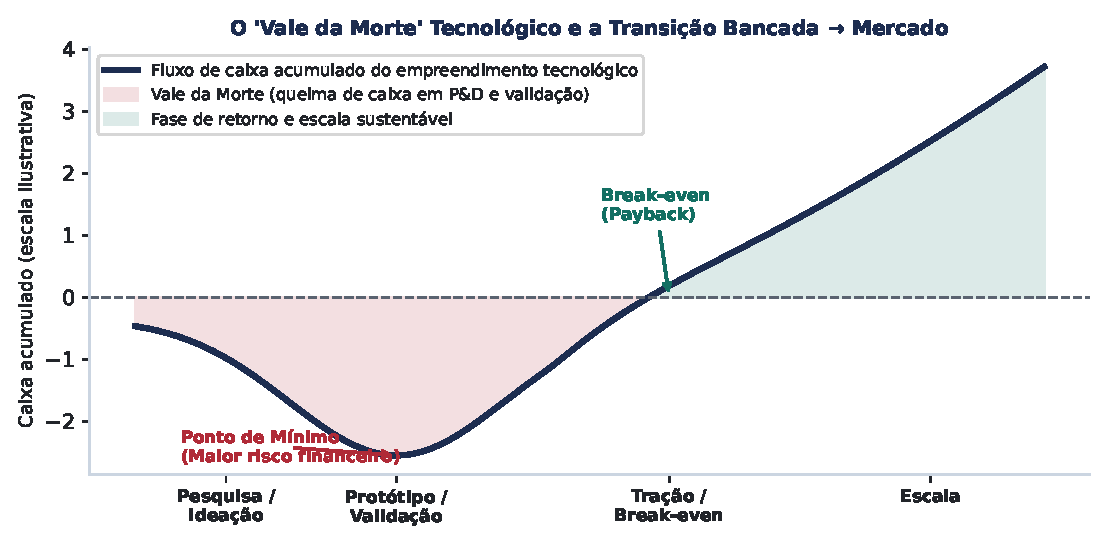
\includegraphics[width=0.90\textwidth]{figures/fig07_vale_da_morte.pdf}
  \caption{Curva J do fluxo de caixa acumulado, Vale da Morte Tecnológico e articulação com a escala de maturidade TRL 1–9.}
  \label{fig:07_vale_morte}
\end{figure}

\begin{boxFormula}[Modelo do Fluxo de Caixa Acumulado e \textit{Payback} no Vale da Morte]
  Considere um empreendimento tecnológico com fluxos de caixa líquidos anuais $FC_t$ para $t = 0, 1, \dots, n$. O fluxo de caixa acumulado no período $t$, denotado por $FCA_t$, é dado pela soma sequencial dos fluxos desde o instante inicial:
  \[
    FCA_t = \sum_{k=0}^{t} FC_k = FCA_{t-1} + FC_t, \quad \text{com } FCA_0 = FC_0.
  \]
  A profundidade máxima do Vale da Morte ($V_{\text{máx}}$) corresponde ao menor valor assumido pelo fluxo acumulado enquanto negativo:
  \[
    V_{\text{máx}} = \min_{t} \{FCA_t\}.
  \]
  O prazo de retorno simples (\textit{payback}) ocorre no intervalo entre o último período $t^*$ em que $FCA_{t^*} < 0$ e o período seguinte $t^* + 1$ em que $FCA_{t^*+1} \ge 0$, sendo interpolado linearmente por:
  \[
    \text{Payback} = t^* + \frac{|FCA_{t^*}|}{FC_{t^*+1}}.
  \]
  Note que a interpolação assume distribuição uniforme das entradas líquidas ao longo do ano $t^*+1$.
\end{boxFormula}

\etapa{4}{Estudos de Caso e Exemplos Resolvidos em 7 Passos}

\begin{boxExemplo}{7.1}{Perda Aceitável e Pássaro na Mão em Biofilme de Palma}
  \passoEnunciado{Uma pesquisadora egressa de mestrado desenvolveu um biofilme comestível à base de mucilagem de palma forrageira para ampliar a vida de prateleira de mangas no Vale do São Francisco. Ela avalia se deve buscar financiamento integral para uma planta piloto antes de testar clientes (\textit{Causation}) ou iniciar por validação enxuta (\textit{Effectuation}).}
  \passoDados{Reserva financeira pessoal disponível: R\$\,18.000,00. Acesso conveniado ao laboratório universitário de alimentos por 6 meses a custo zero de aluguel. Disponibilidade de dedicação: 15 horas semanais, mantendo bolsa de pesquisa de R\$\,3.200,00/mês. Orçamento de planta piloto completa (cenário \textit{Causation}): R\$\,140.000,00. Custo de produzir e testar 30 lotes-piloto com 3 cooperativas locais de fruticultura: R\$\,12.000,00.}
  \passoPedido{Comparar a exposição financeira entre as duas lógicas, calcular a margem de segurança da reserva pessoal sob a lógica efetuacional e identificar os princípios de Sarasvathy mobilizados.}
  \passoMetodo{Aplicação dos princípios \textit{Bird-in-Hand} (meios próprios), \textit{Affordable Loss} (perda aceitável) e \textit{Crazy Quilt} (parceria com cooperativas).}
  \passoContas{
    No cenário \textit{Causation}, o desembolso exigido de R\$\,140.000,00 supera a reserva pessoal em:
    \[
      \text{Déficit de capital} = 140.000,00 - 18.000,00 = \text{R\$\,122.000,00}.
    \]
    Além disso, abandonar a bolsa para dedicação integral sem validação comercial geraria custo de oportunidade de $6 \times 3.200,00 = \text{R\$\,19.200,00}$ no semestre.
    No cenário \textit{Effectuation}, a empreendedora fixa a perda aceitável em R\$\,12.000,00 (insumos para 30 lotes-piloto e análises físico-químicas básicas), preservando uma reserva de segurança de:
    \[
      \text{Reserva preservada} = 18.000,00 - 12.000,00 = \text{R\$\,6.000,00} \quad (33{,}33\% \text{ da reserva}).
    \]
    As 3 cooperativas fornecem as frutas e o espaço de câmara fria para teste em troca de acesso prioritário à tecnologia (pré-compromisso).
  }
  \passoResposta{A abordagem efetuacional reduz a necessidade imediata de capital em 91{,}43\% (de R\$\,140.000,00 para R\$\,12.000,00), preserva R\$\,6.000,00 de reserva e evita R\$\,19.200,00 de perda de renda no semestre inicial.}
  \passoVerificacao{Economicidade e aderência territorial estão preservadas: o laboratório universitário e as cooperativas locais funcionam como amortecedores do risco tecnológico sem endividamento precoce.}
\end{boxExemplo}

\begin{boxExemplo}{7.2}{Mapeamento da Curva J, Vale da Morte e \textit{Payback} em Sensoriamento IoT}
  \passoEnunciado{Uma startup de Feira de Santana desenvolve nós sensores IoT de baixo custo para monitoramento de umidade do solo em perímetros irrigados. O projeto encontra-se em transição do nível TRL 4 para TRL 7.}
  \passoDados{Fluxos de caixa líquidos anuais projetados (em R\$): Ano 0 = $-85.000$; Ano 1 = $-130.000$; Ano 2 = $-45.000$; Ano 3 = $+90.000$; Ano 4 = $+195.000$; Ano 5 = $+260.000$.}
  \passoPedido{Calcular o fluxo de caixa acumulado ano a ano, identificar o ano e o valor do fundo do Vale da Morte e determinar o \textit{payback} simples do projeto.}
  \passoMetodo{Cálculo recursivo de $FCA_t = FCA_{t-1} + FC_t$ e interpolação linear do \textit{payback}.}
  \passoContas{
    Calculando o fluxo acumulado período a período:
    \begin{itemize}[leftmargin=1.4em, itemsep=1pt]
      \item Ano 0: $FCA_0 = -85.000$
      \item Ano 1: $FCA_1 = -85.000 + (-130.000) = -215.000$
      \item Ano 2: $FCA_2 = -215.000 + (-45.000) = -260.000$
      \item Ano 3: $FCA_3 = -260.000 + 90.000 = -170.000$
      \item Ano 4: $FCA_4 = -170.000 + 195.000 = +25.000$
      \item Ano 5: $FCA_5 = +25.000 + 260.000 = +285.000$
    \end{itemize}
    O menor valor acumulado ocorre no Ano 2, com $V_{\text{máx}} = -\text{R\$\,260.000,00}$. Como $FCA_3 = -170.000 < 0$ e $FCA_4 = +25.000 > 0$, o ponto de equilíbrio acumulado ocorre durante o Ano 4 ($t^* = 3$):
    \[
      \text{Payback} = 3 + \frac{|-170.000|}{195.000} = 3 + 0{,}8718 \approx 3{,}87\text{ anos} \quad (\text{cerca de } 46{,}5\text{ meses}).
    \]
  }
  \passoResposta{O fundo do Vale da Morte ocorre no Ano 2, exigindo cobertura acumulada de caixa de R\$\,260.000,00; o \textit{payback} simples é atingido em 3{,}87 anos.}
  \passoVerificacao{O perfil em J é coerente com EBTs de hardware agrícola: os dois primeiros anos concentram prototipagem em campo e homologação (TRL 4–6), e o capital mínimo necessário para não quebrar antes da virada é de pelo menos R\$\,260.000,00.}
\end{boxExemplo}

\begin{boxExemplo}{7.3}{Nexo Indivíduo–Oportunidade na Cadeia do Sisal}
  \passoEnunciado{Dois empreendedores avaliam implantar uma unidade de extração de nanocelulose a partir de resíduos do desfibramento do sisal em Valente (BA). O Empreendedor A é engenheiro químico com 8 anos de atuação técnica em cooperativas sisaleiras; o Empreendedor B é gestor financeiro da capital sem experiência prévia na cadeia agrícola.}
  \passoDados{Acesso a fornecedores de resíduo: A obtém matéria-prima via acordo cooperativo a R\$\,40,00/t; B precisa contratar intermediários a R\$\,110,00/t. Demanda mensal de resíduo: 50 toneladas. Custo mensal de consultoria técnica externa para suprir desconhecimento de processo: R\$\,0,00 para A e R\$\,6.500,00 para B.}
  \passoPedido{Quantificar a vantagem de custo operacional mensal conferida pelo conhecimento prévio e pelas redes territoriais no nexo indivíduo–oportunidade.}
  \passoMetodo{Comparação direta de custos operacionais vinculados à assimetria de informação e conhecimento tácito (Shane \& Venkataraman, 2000).}
  \passoContas{
    Custo mensal com matéria-prima:
    \[
      \text{Custo MP}_A = 50 \times 40{,}00 = \text{R\$\,2.000,00}, \qquad \text{Custo MP}_B = 50 \times 110{,}00 = \text{R\$\,5.500,00}.
    \]
    Somando a consultoria técnica exigida pela ausência de conhecimento prévio:
    \[
      \text{Custo Total}_A = 2.000,00 + 0 = \text{R\$\,2.000,00/mês},
    \]
    \[
      \text{Custo Total}_B = 5.500,00 + 6.500,00 = \text{R\$\,12.000,00/mês}.
    \]
    A diferença mensal é de $12.000,00 - 2.000,00 = \text{R\$\,10.000,00/mês}$ (ou R\$\,120.000,00/ano).
  }
  \passoResposta{O nexo indivíduo–oportunidade enraizado no território gera uma economia operacional de R\$\,10.000,00 mensais para o Empreendedor A.}
  \passoVerificacao{O resultado explica empiricamente por que oportunidades tecnológicas territoriais são mais viáveis quando lideradas por agentes com conhecimento tácito da cadeia local ou em sociedade com eles.}
\end{boxExemplo}

\begin{boxExemplo}{7.4}{Orçamento Escalonado por Níveis de Maturidade TRL 3 a 7}
  \passoEnunciado{Um grupo de pesquisa em biotecnologia ambiental planeja levar um biofertilizante microencapsulado da prova de conceito em bancada (TRL 3) até a demonstração em propriedade agrícola real (TRL 7).}
  \passoDados{Custos estimados por transição de estágio: TRL 3$\to$4 = R\$\,35.000,00; TRL 4$\to$5 = R\$\,65.000,00; TRL 5$\to$6 = R\$\,120.000,00; TRL 6$\to$7 = R\$\,180.000,00. Um edital de subvenção econômica financia 75\% do orçamento total, e investidores-anjo cobrem os 25\% restantes.}
  \passoPedido{Calcular o orçamento total da travessia TRL 3$\to$7, o percentual concentrado na faixa crítica do Vale da Morte (TRL 4$\to$6) e a divisão de fontes de financiamento.}
  \passoMetodo{Soma segmentada por estágio de maturidade tecnológica e rateio proporcional.}
  \passoContas{
    Orçamento total:
    \[
      C_{\text{total}} = 35.000 + 65.000 + 120.000 + 180.000 = \text{R\$\,400.000,00}.
    \]
    Parcela correspondente às transições TRL 4$\to$5 e TRL 5$\to$6:
    \[
      C_{\text{4--6}} = 65.000 + 120.000 = \text{R\$\,185.000,00} \implies \frac{185.000}{400.000} = 0{,}4625 = 46{,}25\%.
    \]
    Parcela da subvenção econômica (75\%) e do investimento-anjo (25\%):
    \[
      \text{Subvenção} = 400.000 \times 0{,}75 = \text{R\$\,300.000,00}, \qquad \text{Anjo} = 400.000 \times 0{,}25 = \text{R\$\,100.000,00}.
    \]
  }
  \passoResposta{O orçamento total é de R\$\,400.000,00, com 46{,}25\% concentrados entre TRL 4 e TRL 6, coberto por R\$\,300.000,00 de subvenção e R\$\,100.000,00 de aporte-anjo.}
  \passoVerificacao{Note que os custos crescem monotonicamente com a escala do ambiente de teste (bancada para campo), justificando a combinação entre recurso público não reembolsável e capital privado paciente.}
\end{boxExemplo}

\begin{boxExemplo}{7.5}{Reconfiguração Efetuacional por Contingência (Princípio da Limonada)}
  \passoEnunciado{Uma startup desenvolveu um filtro cerâmico poroso para dessalinização de água salobra em comunidades rurais do Semiárido. Durante os testes em campo (TRL 6), constatou-se que a vazão obtida era 40\% inferior à necessária para abastecimento humano contínuo, inviabilizando o contrato original com a companhia estadual de saneamento.}
  \passoDados{A mesma cerâmica apresentou retenção de 96\% de corantes têxteis e óleos emulsionados em ensaios paralelos. Custo já investido (afundado): R\$\,90.000,00. Custo adicional para adaptar o módulo ao tratamento de efluentes de pequenas lavanderias industriais da região: R\$\,25.000,00. Receita anual potencial em 15 lavanderias locais: R\$\,11.000,00/lavanderia.}
  \passoPedido{Avaliar a decisão segundo o princípio da Limonada (\textit{Effectuation}) e calcular o retorno incremental sobre o novo aporte necessário.}
  \passoMetodo{Desconsideração de custos afundados (\textit{sunk costs}), reorientação estratégica pela contingência e cálculo de receita potencial incremental.}
  \passoContas{
    Os R\$\,90.000,00 já gastos constituem custo afundado e não devem condicionar a decisão futura. O investimento incremental exigido para pivotar para o mercado de efluentes têxteis é de R\$\,25.000,00. A receita bruta anual potencial com as 15 lavanderias regionais é:
    \[
      R_{\text{anual}} = 15 \times 11.000,00 = \text{R\$\,165.000,00/ano}.
    \]
    Comparando a receita anual potencial com o aporte incremental de adaptação:
    \[
      \frac{165.000}{25.000} = 6{,}6\text{ vezes o capital incremental necessário para a adaptação}.
    \]
  }
  \passoResposta{Aplicando o princípio da Limonada, a equipe aproveita a propriedade filtrante descoberta na falha de vazão para abrir um mercado industrial regional de R\$\,165.000,00/ano com aporte incremental de R\$\,25.000,00.}
  \passoVerificacao{A decisão evita o abandono prematuro do ativo tecnológico e demonstra como o diálogo com demandas produtivas do território transforma limitações técnicas em novos modelos de negócio.}
\end{boxExemplo}

\etapa{5}{Armadilhas Conceituais e Erros Mais Comuns}

\begin{boxErro}[Erro 1 — Confundir \textit{Effectuation} com Improvisação sem Método]
  Assumir que a lógica efetuacional dispensa disciplina analítica, registros financeiros ou metas verificáveis é um equívoco recorrente. Na realidade, o \textit{Effectuation} substitui a previsão de longo prazo pela experimentação controlada com perda aceitável (\textit{affordable loss}) e compromissos formais com parceiros. Improvisar sem definir o limite de perda leva à exaustão de caixa.
\end{boxErro}

\begin{boxErro}[Erro 2 — Subestimar o Custo da Transição TRL 4 para TRL 7]
  Muitos pesquisadores tratam a obtenção de um protótipo funcional em bancada (TRL 4) como sinônimo de produto pronto para venda. Na prática, certificação regulatória, engenharia de manufatura, embalagem, logística e assistência técnica em ambiente operacional costumam custar de três a dez vezes mais do que a pesquisa inicial de laboratório.
\end{boxErro}

\begin{boxErro}[Erro 3 — Ignorar o Fluxo Acumulado ao Analisar o Vale da Morte]
  Avaliar apenas o resultado positivo de um ano futuro (por exemplo, $+90.000$ no Ano 3) sem somar os déficits acumulados dos anos anteriores induz à falsa impressão de suficiência de caixa. Se o fundo do Vale da Morte exige R\$\,260.000,00 acumulados, o projeto quebrará no Ano 2 mesmo que o Ano 3 seja superavitário.
\end{boxErro}

\begin{boxErro}[Erro 4 — Aplicar Lógica \textit{Causation} Rígida em Mercados Inexistentes]
  Exigir projeções econométricas de cinco anos para uma tecnologia radical sem precedentes de consumo gera apenas ficção numérica. Quando não há série histórica confiável, o uso prematuro de planos rígidos imobiliza capital em premissas não testadas em vez de financiar ciclos curtos de aprendizado.
\end{boxErro}

\etapa{6}{Lista de Exercícios (15 Questões em 3 Níveis)}

\textbf{Nível 1 — Fundamentos Conceituais (Questões 1 a 5)}

\begin{enumerate}[leftmargin=1.5em, itemsep=6pt]
  \item Explique, com base em Shane e Venkataraman (2000), por que a existência de uma nova tecnologia em uma universidade não gera automaticamente um empreendimento sem a mediação do nexo indivíduo–oportunidade.
  \espacoResolucao[1.8cm]

  \item Diferencie os critérios de tomada de decisão das lógicas \textit{Causation} e \textit{Effectuation} quanto ao ponto de partida, à postura diante do risco e ao relacionamento com outros atores do mercado.
  \espacoResolucao[1.8cm]

  \item Associe cada um dos cinco princípios de Sarasvathy (pássaro na mão, perda aceitável, colcha de retalhos, limonada e piloto no avião) a uma ação prática de um grupo de pós-graduandos iniciando uma startup territorial.
  \espacoResolucao[2.0cm]

  \item Descreva o que caracteriza os níveis TRL 3, TRL 6 e TRL 9 e explique por que o Vale da Morte Tecnológico concentra-se tipicamente entre TRL 4 e TRL 6.
  \espacoResolucao[1.8cm]

  \item Por que o fluxo de caixa acumulado descreve uma Curva em J nos empreendimentos de base tecnológica? Indique o significado econômico do ponto mínimo da curva e do cruzamento do eixo horizontal.
  \espacoResolucao[1.8cm]

  \item \textbf{(Nível 2 — Aplicações Numéricas)} Uma startup de biotecnologia apresenta os seguintes fluxos de caixa líquidos anuais (em R\$): Ano 0 = $-60.000$; Ano 1 = $-90.000$; Ano 2 = $-30.000$; Ano 3 = $+75.000$; Ano 4 = $+150.000$. Calcule o fluxo de caixa acumulado para cada ano, o valor do fundo do Vale da Morte e o \textit{payback} simples.
  \espacoResolucao[2.4cm]

  \item Uma empreendedora possui R\$\,25.000,00 de reserva pessoal e define como perda aceitável exatamente 40\% desse valor para validar um aplicativo de rastreabilidade agrícola em 4 meses. Caso o experimento falhe, qual será o valor perdido e qual a reserva preservada? Se o custo de um desenvolvedor terceirizado fosse R\$\,18.000,00, o projeto caberia na perda aceitável?
  \espacoResolucao[2.2cm]

  \item Um projeto de equipamento agroindustrial estima custos de R\$\,40.000,00 (TRL 3$\to$4), R\$\,80.000,00 (TRL 4$\to$5), R\$\,130.000,00 (TRL 5$\to$6) e R\$\,250.000,00 (TRL 6$\to$7). Calcule o orçamento total e a participação percentual da etapa TRL 6$\to$7 no total necessário.
  \espacoResolucao[2.2cm]

  \item Dois projetos concorrem a um fundo territorial. O Projeto Alfa segue lógica \textit{Causation} e exige R\$\,320.000,00 iniciais para montar fábrica antes das vendas. O Projeto Beta usa \textit{Effectuation}, firmando pré-compromisso com uma cooperativa que cede galpão e reduz o investimento inicial em 62{,}5\%. Qual o aporte inicial necessário para o Projeto Beta?
  \espacoResolucao[2.2cm]

  \item Uma equipe obteve fluxo de caixa acumulado de $-\text{R\$\,180.000,00}$ ao final do Ano 2. Nos Anos 3 e 4, os fluxos líquidos positivos são de R\$\,100.000,00 e R\$\,160.000,00, respectivamente. Em quantos anos ocorre o \textit{payback} simples?
  \espacoResolucao[2.2cm]

  \item \textbf{(Nível 3 — Análise Territorial e Estratégica)} Analise como a presença de uma universidade estadual e de cooperativas agrícolas em um território semiárido altera os princípios "pássaro na mão" e "colcha de retalhos" para um pesquisador local em comparação a um empreendedor isolado em região sem infraestrutura de CT\&I.
  \espacoResolucao[2.2cm]

  \item Um projeto de dessalinização solar apresenta $FC_0 = -100.000$, $FC_1 = -140.000$, $FC_2 = +60.000$, $FC_3 = +120.000$ e $FC_4 = +150.000$. Caso um edital de subvenção econômica cubra R\$\,120.000,00 no Ano 1 (reduzindo o déficit do Ano 1 para $-20.000$), em quanto diminui a profundidade do Vale da Morte e qual passa a ser o novo \textit{payback} simples?
  \espacoResolucao[2.5cm]

  \item Discuta em que momento do ciclo de vida de uma EBT a equipe deve migrar da predominância de \textit{Effectuation} para a incorporação sistemática de ferramentas de \textit{Causation}, justificando os riscos de realizar essa transição cedo demais ou tarde demais.
  \espacoResolucao[2.2cm]

  \item Uma pesquisadora gastou R\$\,50.000,00 desenvolvendo um sensor para o setor petrolífero, mas o cliente cancelou o projeto por mudança regulatória. Para adaptar o sensor ao monitoramento de barragens de rejeitos minerais na Bahia, são necessários R\$\,30.000,00 adicionais, com receita líquida estimada de R\$\,45.000,00/ano durante 3 anos. Desconsiderando custos afundados, a adaptação é atrativa? Justifique quantitativamente.
  \espacoResolucao[2.4cm]

  \item Elabore uma matriz comparativa indicando como três falhas típicas no Vale da Morte (ausência de validação com usuário, falta de capital paciente e subestimação de certificação) podem ser mitigadas articulando \textit{Effectuation} e instrumentos territoriais de fomento.
  \espacoResolucao[2.4cm]
\end{enumerate}

\etapa{7}{Questões Autorais Estilo Pós-Graduação / Concursos de CT\&I}

\begin{enumerate}[leftmargin=1.5em, itemsep=6pt]
  \item \textbf{(Estilo ANPAD / Gestão da Inovação)} Considere as assertivas sobre o processo empreendedor segundo Shane \& Venkataraman (2000) e Sarasvathy (2001):
  I. O nexo indivíduo–oportunidade sustenta que oportunidades empreendedoras são percebidas igualmente por todos os agentes econômicos que têm acesso à mesma informação pública.
  II. Na lógica \textit{Effectuation}, o princípio da perda aceitável substitui o cálculo do retorno máximo esperado como critério de decisão em ambientes de incerteza knightiana.
  III. A lógica \textit{Causation} é inadequada para qualquer etapa de uma empresa, devendo ser abandonada mesmo após a consolidação do mercado.
  Assinale a alternativa correta:
  \begin{alternativas}
    \item Apenas I está correta.
    \item Apenas II está correta.
    \item Apenas I e II estão corretas.
    \item Apenas II e III estão corretas.
    \item I, II e III estão corretas.
  \end{alternativas}
  \espacoResolucao[1.5cm]

  \item \textbf{(Estilo Concurso Analista de CT\&I — FINEP/FAPs)} Uma empresa de base tecnológica apresenta os fluxos de caixa líquidos anuais (em milhares de R\$): Ano 0 = $-120$; Ano 1 = $-180$; Ano 2 = $-60$; Ano 3 = $+150$; Ano 4 = $+210$; Ano 5 = $+240$. Sobre o perfil da Curva J desse empreendimento, assinale a alternativa correta:
  \begin{alternativas}
    \item O fundo do Vale da Morte ocorre no Ano 1, com déficit acumulado de R\$\,300 mil.
    \item O fundo do Vale da Morte ocorre no Ano 2, com déficit acumulado de R\$\,360 mil, e o \textit{payback} simples ocorre exatamente ao final do Ano 4.
    \item O fundo do Vale da Morte ocorre no Ano 2, com déficit acumulado de R\$\,360 mil, e o \textit{payback} simples ocorre entre o Ano 3 e o Ano 4.
    \item O \textit{payback} simples ocorre aos 3{,}50 anos.
    \item O projeto nunca atinge saldo acumulado positivo até o Ano 5.
  \end{alternativas}
  \espacoResolucao[1.6cm]

  \item \textbf{(Estilo Discursiva de Seleção de Mestrado / PPGPT)} Analise criticamente a seguinte afirmação: ``O Vale da Morte Tecnológico resulta exclusivamente da escassez de crédito bancário comercial nos países em desenvolvimento''. Em sua resposta, articule os conceitos de maturidade tecnológica (TRL), incerteza knightiana e o papel das alianças efetuacionais (\textit{crazy quilt}) na superação dessa fase.
  \espacoResolucao[2.5cm]
\end{enumerate}

\begin{boxDica}[Contraponto Crítico e Prática Territorial (AV3)]
  Ao estruturar o seu Projeto Final (AV3), evite apresentar um plano de negócios puramente preditivo se a tecnologia ou o arranjo territorial ainda estiver em fase de validação (TRL 3–5). Explicite quais são os seus meios atuais (\textit{Bird-in-Hand}), qual é a perda aceitável para o primeiro ciclo de testes e quais cooperativas, laboratórios ou prefeituras compõem a sua colcha de retalhos (\textit{Crazy Quilt}).
\end{boxDica}

\clearpage
\etapa{8}{Gabarito Integralmente Comentado (Exercícios 1 a 18)}

\begin{boxGabarito}[Resolução Completa dos Exercícios da Etapa 6 (1 a 15) e Etapa 7 (16 a 18)]
  \begin{enumerate}[leftmargin=1.5em, itemsep=4pt]
    \item \textbf{Resposta:} Segundo Shane e Venkataraman (2000), a oportunidade tecnológica objetiva precisa ser percebida, avaliada e explorada por um indivíduo ou equipe dotado de conhecimento prévio e capacidade cognitiva para conectar a solução técnica a uma demanda real. Sem esse nexo, a patente ou protótipo permanece ocioso na bancada.
    \item \textbf{Resposta:} \textit{Causation} parte de uma meta fixa, decide pela maximização do retorno esperado e vê outros atores principalmente como concorrentes a analisar. \textit{Effectuation} parte dos meios disponíveis, decide pela perda aceitável e busca parcerias de pré-compromisso para co-criar o mercado.
    \item \textbf{Resposta:} \textit{Pássaro na mão}: mapear competências do grupo, equipamentos do laboratório e contatos locais; \textit{Perda aceitável}: limitar gastos iniciais a uma reserva definida; \textit{Colcha de retalhos}: envolver cooperativa ou prefeitura como parceira de teste; \textit{Limonada}: adaptar o produto caso o teste revele uso alternativo; \textit{Piloto no avião}: conduzir negociações ativas em vez de esperar tendências externas.
    \item \textbf{Resposta:} TRL 3 representa a prova de conceito experimental em laboratório; TRL 6, a demonstração de protótipo em ambiente relevante real; TRL 9, o sistema operando comercialmente. Entre TRL 4 e 6 ocorre o Vale da Morte porque os editais de pesquisa básica já terminaram e o capital privado ainda exige comprovação comercial para investir.
    \item \textbf{Resposta:} A curva tem formato de J porque os desembolsos iniciais em P\&D, prototipagem e certificação geram fluxos líquidos negativos antes das vendas recorrentes. O ponto mínimo indica a necessidade máxima de capital acumulado para atravessar o Vale da Morte; o cruzamento do eixo horizontal indica o \textit{payback} simples (recuperação do capital investido).
    \item \textbf{Resposta:} $FCA_0 = -60.000$; $FCA_1 = -60.000 - 90.000 = -150.000$; $FCA_2 = -150.000 - 30.000 = -180.000$ (fundo do Vale da Morte); $FCA_3 = -180.000 + 75.000 = -105.000$; $FCA_4 = -105.000 + 150.000 = +45.000$. O \textit{payback} ocorre no Ano 4: $3 + 105.000 / 150.000 = 3 + 0{,}70 = 3{,}70\text{ anos}$.
    \item \textbf{Resposta:} Perda aceitável = $25.000 \times 0{,}40 = \text{R\$\,10.000,00}$. Reserva preservada = $25.000 - 10.000 = \text{R\$\,15.000,00}$. A contratação de R\$\,18.000,00 excederia a perda aceitável em R\$\,8.000,00, não devendo ser realizada nessa configuração.
    \item \textbf{Resposta:} Orçamento total = $40.000 + 80.000 + 130.000 + 250.000 = \text{R\$\,500.000,00}$. Participação de TRL 6$\to$7 = $250.000 / 500.000 = 0{,}50 = 50\%$.
    \item \textbf{Resposta:} Redução = $320.000 \times 0{,}625 = \text{R\$\,200.000,00}$. Aporte inicial necessário para Beta = $320.000 - 200.000 = \text{R\$\,120.000,00}$.
    \item \textbf{Resposta:} Ao fim do Ano 2, $FCA_2 = -180.000$. No Ano 3, $FCA_3 = -180.000 + 100.000 = -80.000$. No Ano 4, $FCA_4 = -80.000 + 160.000 = +80.000$. Logo, $\text{Payback} = 3 + 80.000 / 160.000 = 3{,}50\text{ anos}$.
    \item \textbf{Resposta:} A universidade amplia o "pássaro na mão" (acesso a laboratórios, orientação científica e bolsistas) e as cooperativas viabilizam a "colcha de retalhos" (espaços de teste, matéria-prima e primeiros usuários), reduzindo o custo de experimentação frente a um empreendedor isolado.
    \item \textbf{Resposta:} Cenário original: $FCA_0 = -100.000$; $FCA_1 = -240.000$ (fundo); $FCA_2 = -180.000$; $FCA_3 = -60.000$; $FCA_4 = +90.000$. Payback original = $3 + 60.000 / 150.000 = 3{,}40\text{ anos}$. Com subvenção de R\$\,120.000 no Ano 1 ($FC_1 = -20.000$): $FCA_0 = -100.000$; $FCA_1 = -120.000$ (novo fundo); $FCA_2 = -60.000$; $FCA_3 = +60.000$. A profundidade do Vale da Morte cai em R\$\,120.000,00 (de R\$\,240.000 para R\$\,120.000, redução de 50\%), e o novo \textit{payback} cai para $2 + 60.000 / 120.000 = 2{,}50\text{ anos}$.
    \item \textbf{Resposta:} A transição deve ocorrer após a validação do problema, da solução e dos primeiros clientes pagantes (TRL 6–7). Migrar cedo demais para \textit{Causation} engessa o negócio em premissas falsas; migrar tarde demais impede a captação de crédito estruturado e a gestão de escala.
    \item \textbf{Resposta:} Sim. Os R\$\,50.000,00 iniciais são custo afundado. O investimento incremental é de R\$\,30.000,00 para gerar R\$\,45.000,00/ano $\times$ 3 anos = R\$\,135.000,00 de receita líquida acumulada, gerando saldo incremental positivo de R\$\,105.000,00 e retorno do aporte adicional em $30.000 / 45.000 \approx 0{,}67\text{ ano}$ (8 meses).
    \item \textbf{Resposta:} (1) Ausência de validação $\to$ mitigada com testes rápidos e pré-compromissos com usuários locais (\textit{Crazy Quilt}); (2) Falta de capital paciente $\to$ mitigada por subvenções estaduais/federais combinadas com perda aceitável; (3) Subestimação de certificação $\to$ mitigada por parcerias com laboratórios credenciados de ICTs desde TRL 4.
    \item \textbf{Questão 16 (Etapa 7) — Gabarito: (B).} I é falsa porque o conhecimento prévio é assimétrico, logo nem todos percebem a mesma oportunidade. II é verdadeira. III é falsa porque \textit{Causation} é útil na fase de escala e previsibilidade.
    \item \textbf{Questão 17 (Etapa 7) — Gabarito: (B).} $FCA_0 = -120$; $FCA_1 = -300$; $FCA_2 = -360$ (fundo do Vale da Morte); $FCA_3 = -210$; $FCA_4 = -210 + 210 = 0$. Logo, o \textit{payback} simples ocorre exatamente ao final do Ano 4 ($4{,}00$ anos).
    \item \textbf{Questão 18 (Etapa 7) — Espelho Discursivo:} A resposta deve refutar o reducionismo creditício, explicando que entre TRL 4 e 6 há elevada incerteza tecnológica e de mercado (incerteza knightiana), que impede a precificação tradicional de risco por bancos comerciais. Deve ainda demonstrar como editais de subvenção e alianças efetuacionais (\textit{crazy quilt}) com usuários-piloto compartilham o risco nessa travessia.
  \end{enumerate}
\end{boxGabarito}

\begin{boxResumo}
  \begin{itemize}[leftmargin=1.4em, itemsep=2pt]
    \item O empreendedorismo emerge do nexo entre indivíduos com conhecimento prévio/redes territoriais e oportunidades econômicas ou socioambientais.
    \item Sob incerteza radical, a lógica \textit{Effectuation} (pássaro na mão, perda aceitável, colcha de retalhos, limonada, piloto no avião) preserva caixa e acelera o aprendizado.
    \item A transição bancada–mercado forma uma Curva J cujo ponto mínimo define o Vale da Morte Tecnológico (TRL 4–6), exigindo planejamento de caixa acumulado e instrumentos híbridos de fomento.
  \end{itemize}
\end{boxResumo}

\begin{boxTeste}
  \begin{enumerate}[leftmargin=1.5em, itemsep=4pt]
    \item (\V/\F) Na lógica \textit{Effectuation}, o empreendedor fixa primeiro uma meta de participação de mercado em cinco anos e depois busca o capital total necessário para atingi-la.
    \item (\V/\F) O princípio da perda aceitável recomenda limitar o investimento experimental ao montante máximo que o empreendedor pode perder sem comprometer sua sobrevivência.
    \item (\V/\F) Um projeto com $FC_0 = -50.000$, $FC_1 = -70.000$ e $FC_2 = +120.000$ apresenta fundo do Vale da Morte de $-\text{R\$\,120.000,00}$ no Ano 1 e atinge \textit{payback} simples exatamente ao final do Ano 2.
    \item (\V/\F) Na escala TRL, o nível 3 corresponde à operação comercial plena em escala industrial.
  \end{enumerate}
  \begin{boxGabarito}[Respostas do Checkpoint — Capítulo 7]
    \textbf{1: \F} (Essa é a lógica \textit{Causation}). \quad \textbf{2: \V}. \quad \textbf{3: \V} ($FCA_1 = -120.000$; $FCA_2 = 0$). \quad \textbf{4: \F} (Operação comercial plena é TRL 9; TRL 3 é prova de conceito em laboratório).
  \end{boxGabarito}
\end{boxTeste}

\chapter{Identificação e Análise de Oportunidades Tecnológicas e Territoriais}
\label{cap:08}
\markboth{CAPÍTULO 8: ANÁLISE DE OPORTUNIDADES}{CAPÍTULO 8: ANÁLISE DE OPORTUNIDADES}

\noindent\tagQuant\ \tagTerritorio

\begin{capObjetivos}
  Ao concluir este capítulo, você será capaz de:
  \begin{enumerate}[leftmargin=1.5em, itemsep=2pt]
    \item Distinguir a Teoria da Descoberta da Teoria da Criação de Oportunidades (\textit{Alvarez \& Barney, 2007}) e suas implicações para a estratégia empresarial.
    \item Identificar sinais territoriais de oportunidade a partir das sete fontes de inovação sistematizadas por Peter Drucker (1985).
    \item Calcular e cruzar o dimensionamento de mercado \textbf{TAM, SAM e SOM} pelas abordagens \textit{top-down} e \textit{bottom-up}.
    \item Avaliar instrumentos de \textbf{Propriedade Intelectual (PI)}, patentes, modelos de utilidade, registro de software, cultivares, marcas e segredo industrial, e a função da busca de anterioridade.
  \end{enumerate}
\end{capObjetivos}

\begin{capRevisao}
  Retome três noções essenciais dos capítulos anteriores:
  \begin{itemize}[leftmargin=1.5em, itemsep=2pt]
    \item \textbf{Nexo Indivíduo–Oportunidade:} a identificação de oportunidades depende tanto das assimetrias do mercado quanto do conhecimento prévio acumulado pelo agente.
    \item \textbf{Incerteza vs. Risco:} oportunidades em mercados conhecidos permitem estimativas probabilísticas; oportunidades em mercados inéditos requerem construção iterativa.
    \item \textbf{Indicações Geográficas (IGs) e Ativos Territoriais:} conforme visto na Unidade I, ativos específicos de um território (saberes, biodiversidade, cadeias produtivas) podem gerar diferenciação não replicável.
  \end{itemize}
\end{capRevisao}

\etapa{3}{Explicação Teórica, Vocabulário Prévio e Modelos}

\begin{boxSimbolo}[Vocabulário Conceitual e Símbolos do Capítulo 8]
  \begin{tabularx}{\textwidth}{@{}l >{\raggedright\arraybackslash}X@{}}
    \textbf{TAM} & \textit{Total Addressable Market}: demanda total máxima global ou nacional para uma categoria de solução. \\
    \textbf{SAM} & \textit{Serviceable Available Market}: parcela do TAM alcançável pelo modelo de negócio, restrições geográficas e recorte regulatório. \\
    \textbf{SOM} & \textit{Serviceable Obtainable Market}: parcela realista do SAM que o empreendimento consegue capturar no horizonte de 3 a 5 anos dada sua capacidade produtiva e comercial. \\
    \textbf{PI / INPI} & Propriedade Intelectual e Instituto Nacional da Propriedade Industrial. \\
    \textbf{PI vs. MU} & Patente de Invenção (vigência de 20 anos) e Modelo de Utilidade (vigência de 15 anos). \\
    \textbf{FTO} & \textit{Freedom to Operate}: análise que verifica se uma tecnologia pode ser comercializada sem infringir patentes vigentes de terceiros. \\
  \end{tabularx}
\end{boxSimbolo}

\section{Teoria da Descoberta vs. Teoria da Criação (Alvarez \& Barney, 2007)}

Uma questão central na estratégia empreendedora indaga se as oportunidades existem objetivamente no ambiente econômico aguardando quem as encontre, ou se são construídas pelas ações dos próprios empreendedores. Sharon Alvarez e Jay Barney (2007) organizaram esse debate em duas teorias complementares.

Na \textbf{Teoria da Descoberta}, as oportunidades existem de forma independente dos empreendedores, originadas por choques exógenos como novas descobertas científicas, mudanças demográficas, alterações regulatórias ou falhas de mercado. O contexto decisório é de \textbf{risco}: é possível coletar dados, estimar o tamanho da demanda e formular planos baseados em lógica \textit{Causation}. O empreendedor diferencia-se pela atenção alerta (\textit{alertness}) para enxergar lacunas antes dos concorrentes.

Na \textbf{Teoria da Criação}, as oportunidades emergem de forma endógena à medida que empreendedores interagem com clientes, fornecedores e instituições, testando hipóteses e modificando preferências. O contexto decisório é de \textbf{incerteza knightiana}, pois inexistem dados prévios confiáveis para pesquisa de mercado tradicional. Nesse cenário, prevalece a lógica \textit{Effectuation}, na qual o aprendizado iterativo molda simultaneamente o produto e o mercado.

\begin{center}
\renewcommand{\arraystretch}{1.22}
\small
\begin{tabularx}{\textwidth}{@{}l >{\raggedright\arraybackslash}X >{\raggedright\arraybackslash}X@{}}
  \toprule
  \rowcolor{etIndigo}
  \textcolor{white}{\bfseries Critério} & \textcolor{white}{\bfseries Teoria da Descoberta} & \textcolor{white}{\bfseries Teoria da Criação} \\
  \midrule
  Natureza da oportunidade & Objetiva, gerada por choques exógenos. & Endógena, construída na ação social e técnica. \\
  \rowcolor{bgGray}
  Condição de informação & Risco mensurável por dados históricos. & Incerteza radical sem série histórica. \\
  Estratégia recomendada & Planejamento preditivo (\textit{Causation}). & Experimentação iterativa (\textit{Effectuation}). \\
  \rowcolor{bgGray}
  Exemplo territorial & Software para atender nova exigência fiscal agrícola. & Criação de mercado para créditos de biodiversidade da Caatinga. \\
  \bottomrule
\end{tabularx}
\end{center}

\section{As 7 Fontes de Inovação de Drucker (1985) e Sinais Territoriais}

Para sistematizar a observação de oportunidades sem depender de inspiração aleatória, Peter Drucker (1985) identificou sete fontes de oportunidade inovadora, divididas entre quatro fontes internas ao setor produtivo e três fontes externas situadas no ambiente social e intelectual. No planejamento territorial, as quatro primeiras emergem diretamente da dinâmica das cadeias produtivas locais. O \textbf{inesperado} manifesta-se em sucessos ou fracassos imprevistos de produtos regionais, como ocorre quando um subproduto descartado na agroindústria passa a atrair procura cosmética. A \textbf{incongruência} revela o descompasso entre a realidade econômica de um território e as premissas vigentes, visível em regiões com elevada produção primária e baixíssima agregação de valor local. De modo complementar, a \textbf{necessidade de processo} aponta gargalos técnicos específicos que travam o rendimento regional, a exemplo da elevada perda pós-colheita decorrente da falta de pré-resfriamento móvel, enquanto as \textbf{mudanças na estrutura da indústria ou do mercado} abrem brechas por meio da descentralização logística, da transição energética ou da abertura de compras públicas sustentáveis.

As três fontes externas ampliam esse diagnóstico ao captar transformações demográficas, culturais e científicas que reconfiguram a demanda territorial. As \textbf{mudanças demográficas} abrangem o envelhecimento da população rural, o êxodo ou o retorno de jovens qualificados pela interiorização do ensino superior, alterando a disponibilidade de mão de obra e o perfil de consumo. Já as \textbf{mudanças de percepção} refletem a valorização crescente de rastreabilidade, agroecologia, economia circular e origem territorial certificada por parte dos compradores. Integrando esse conjunto, o \textbf{novo conhecimento} decorre de avanços científicos em biotecnologia, sensoriamento remoto, novos materiais ou inteligência artificial passíveis de adaptação a problemas locais concretos.

\section{Dimensionamento de Mercado: TAM, SAM e SOM}

Identificar uma necessidade real exige quantificar a escala econômica da oportunidade antes de imobilizar capital. O funil \textbf{TAM–SAM–SOM} evita projeções infladas, como reivindicar um percentual arbitrário de um mercado bilionário, e conecta a ambição estratégica à capacidade operacional efetiva da equipe. Conforme ilustra a Figura~\ref{fig:08_tam_sam_som}, o dimensionamento parte da demanda máxima teórica (TAM), aplica filtros geográficos e regulatórios para delimitar o mercado alcançável (SAM) e converge para a fatia realista obtenível (SOM) no horizonte inicial de operação.

\begin{figure}[H]
  \centering
  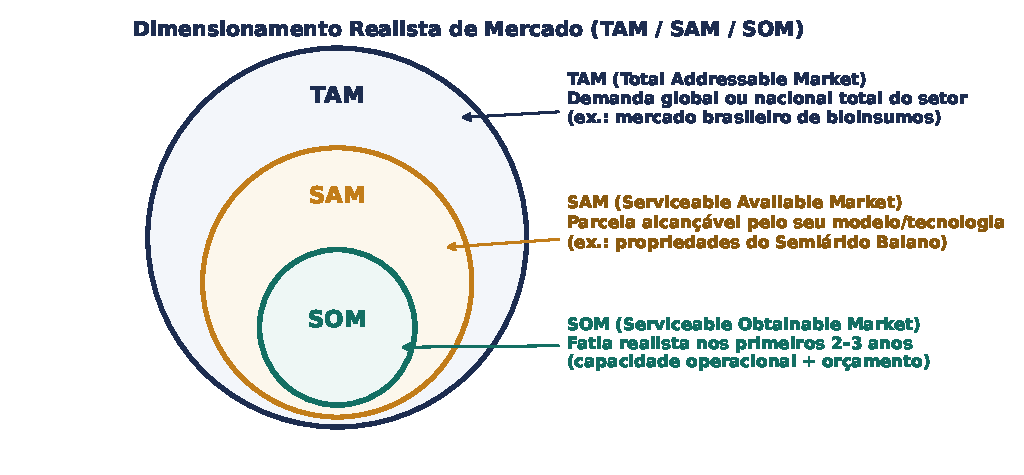
\includegraphics[width=0.90\textwidth]{figures/fig08_tam_sam_som.pdf}
  \caption{Funil de dimensionamento de mercado TAM, SAM e SOM articulando estimativas \textit{top-down} e \textit{bottom-up}.}
  \label{fig:08_tam_sam_som}
\end{figure}

\begin{boxFormula}[Modelagem Quantitativa TAM, SAM e SOM (\textit{Top-Down} e \textit{Bottom-Up})]
  \textbf{1. Abordagem \textit{Top-Down} (de cima para baixo):} parte de dados macroeconômicos ou setoriais agregados e aplica filtros sucessivos de segmentação geográfica e técnica.
  \[
    \text{TAM} = N_{\text{total}} \times T_{\text{anual}}, \qquad
    \text{SAM} = \text{TAM} \times f_{\text{geo}} \times f_{\text{seg}}, \qquad
    \text{SOM}_{\text{TD}} = \text{SAM} \times s_{\text{cap}},
  \]
  onde $N_{\text{total}}$ é o universo potencial de clientes no mercado amplo, $T_{\text{anual}}$ é o gasto médio anual por cliente, $f_{\text{geo}}$ e $f_{\text{seg}}$ são os fatores de recorte geográfico e de aderência ao modelo de negócio, e $s_{\text{cap}}$ é a fatia de mercado (\textit{market share}) realista no horizonte planejado.

  \vspace{4pt}
  \textbf{2. Abordagem \textit{Bottom-Up} (de baixo para cima):} constrói o SOM a partir da capacidade operacional efetiva da equipe, da produção ou dos canais de venda:
  \[
    \text{SOM}_{\text{BU}} = \min\bigl(C_{\text{máx}}, \; N_{\text{alvo}} \times Q_{\text{anual}}\bigr) \times P_{\text{unitário}},
  \]
  onde $C_{\text{máx}}$ é a capacidade máxima anual de entrega ou atendimento, $N_{\text{alvo}}$ é o número de clientes alcançáveis pela força comercial, $Q_{\text{anual}}$ é o volume médio anual por cliente e $P_{\text{unitário}}$ é o preço unitário. A consistência do plano exige verificar se $\text{SOM}_{\text{BU}} \le \text{SAM}$.
\end{boxFormula}

\section{Propriedade Intelectual (PI) na Avaliação de Oportunidades}

Em empreendimentos de base tecnológica, a apropriação dos retornos da inovação depende da estratégia de \textbf{Propriedade Intelectual (PI)}. No Brasil, a proteção industrial é regida principalmente pela Lei nº 9.279/1996 (Lei da Propriedade Industrial), pela Lei nº 9.609/1998 (Software) e pela Lei nº 9.456/1997 (Cultivares). A escolha do ativo de PI equilibra custo, tempo de concessão e risco de engenharia reversa entre diferentes regimes jurídicos. Para invenções técnicas, a \textbf{Patente de Invenção (PI)} protege produtos ou processos inéditos com atividade inventiva e aplicação industrial por 20 anos a partir do depósito, exigindo divulgação pública integral do método no documento patentário, ao passo que o \textbf{Modelo de Utilidade (MU)} resguarda por 15 anos objetos de uso prático com nova forma ou disposição que resulte em melhoria funcional no uso ou fabricação. No domínio digital e biológico, o \textbf{Registro de Programa de Computador (Software)} protege o código-fonte como direito autoral no INPI por 50 anos a partir de 1º de janeiro do ano subsequente à publicação ou criação, enquanto a \textbf{Proteção de Cultivares} junto ao SNPC/MAPA aplica-se a novas variedades vegetais desenvolvidas por melhoramento genético, sendo vital para a bioeconomia regional.

Quando a vantagem competitiva reside na identidade comercial, na origem ou no sigilo de processo, outros instrumentos tornam-se prioritários. As \textbf{Marcas} protegem sinais distintivos por 10 anos renováveis, e as \textbf{Indicações Geográficas (IGs)} vinculam reputação ou qualidade ao território por meio de Indicação de Procedência ou Denominação de Origem. Em contraposição ao registro público, o \textbf{Segredo Industrial} mantém sigilo sobre formulações, parâmetros de processo ou algoritmos internos sem prazo legal de expiração, desde que esses elementos resistam à descoberta por engenharia reversa.

Antes de investir em P\&D ou lançar um produto, é obrigatório realizar a \textbf{busca de anterioridade} em bases públicas (INPI, Espacenet, PATENTSCOPE, Google Patents). Essa busca cumpre duas funções complementares, evitando o desperdício de recursos ao reinventar soluções já existentes no estado da técnica e verificando a \textbf{liberdade de operação (\textit{Freedom to Operate}, FTO)} para assegurar que a comercialização não violará patentes vigentes no território de venda.

\etapa{4}{Estudos de Caso e Exemplos Resolvidos em 7 Passos}

\begin{boxExemplo}{8.1}{Dimensionamento \textit{Top-Down}: Plataforma de Rastreabilidade do Mel}
  \passoEnunciado{Uma startup baiana desenvolve uma plataforma digital de rastreabilidade sanitária e certificação de origem para cooperativas e produtores de mel do Semiárido.}
  \passoDados{Universo nacional estimado de apicultores formais e associados: $N_{\text{total}} = 120.000$ produtores. Assinatura anual da plataforma: $T_{\text{anual}} = \text{R\$\,1.800,00/ano}$. Recorte geográfico e de perfil cooperativado no Nordeste: $f_{\text{geo}} \times f_{\text{seg}} = 25\%$ ($0{,}25$). Meta realista de captura em 3 anos com equipe de 3 consultores territoriais: $s_{\text{cap}} = 4\%$ ($0{,}04$) do SAM.}
  \passoPedido{Calcular o TAM, o SAM e o SOM anual pela abordagem \textit{top-down}, além do número de apicultores pagantes necessários para atingir o SOM.}
  \passoMetodo{Aplicação sequencial das equações \textit{top-down} de TAM, SAM e SOM.}
  \passoContas{
    \[
      \text{TAM} = 120.000 \times 1.800 = \text{R\$\,216.000.000,00/ano}.
    \]
    Aplicando o fator de recorte regional e de aderência ($0{,}25$):
    \[
      \text{SAM} = 216.000.000 \times 0{,}25 = \text{R\$\,54.000.000,00/ano} \quad (30.000\text{ apicultores}).
    \]
    Aplicando a meta de captura ($4\%$ do SAM):
    \[
      \text{SOM}_{\text{TD}} = 54.000.000 \times 0{,}04 = \text{R\$\,2.160.000,00/ano}.
    \]
    O número de apicultores pagantes no SOM é $30.000 \times 0{,}04 = 1.200$ produtores (400 produtores atendidos por consultor).
  }
  \passoResposta{$\text{TAM} = \text{R\$\,216,0 milhões/ano}$; $\text{SAM} = \text{R\$\,54,0 milhões/ano}$; $\text{SOM} = \text{R\$\,2,16 milhões/ano}$ (1.200 produtores).}
  \passoVerificacao{Atender 1.200 apicultores por meio de cooperativas regionais com 3 consultores (cerca de 15 a 20 cooperativas de 60 a 80 associados cada) é operacionalmente factível no horizonte de 3 anos.}
\end{boxExemplo}

\begin{boxExemplo}{8.2}{Dimensionamento \textit{Bottom-Up}: Bioinsumo para Cacauicultura no Sul da Bahia}
  \passoEnunciado{Uma biofábrica emergente no Sul da Bahia produz um biofungicida à base de \textit{Trichoderma} para controle da vassoura-de-bruxa e podridão-parda em lavouras de cacau.}
  \passoDados{Capacidade máxima da biofábrica piloto: $C_{\text{máx}} = 48.000\text{ litros/ano}$. Dose recomendada: $8\text{ litros/ha/ano}$. Área média de cacau por propriedade atendida: $15\text{ ha}$. Preço unitário: $P_{\text{unitário}} = \text{R\$\,45,00/litro}$. Área regional de cacau tecnificado (SAM físico): $180.000\text{ ha}$.}
  \passoPedido{Calcular o SOM anual pela abordagem \textit{bottom-up}, o número máximo de hectares e propriedades atendidas, o SAM financeiro regional e a fatia do SAM representada pelo SOM.}
  \passoMetodo{Cálculo da restrição produtiva \textit{bottom-up} e comparação com o SAM regional.}
  \passoContas{
    Como a capacidade é de $48.000\text{ L/ano}$ e o preço é R\$\,45,00/L, o SOM limitado pela capacidade produtiva é:
    \[
      \text{SOM}_{\text{BU}} = 48.000 \times 45{,}00 = \text{R\$\,2.160.000,00/ano}.
    \]
    Hectares atendidos: $48.000 / 8 = 6.000\text{ ha/ano}$. Propriedades atendidas: $6.000 / 15 = 400\text{ propriedades/ano}$.
    O gasto anual por hectare é $8 \times 45{,}00 = \text{R\$\,360,00/ha}$. Assim, o SAM regional é:
    \[
      \text{SAM} = 180.000 \times 360{,}00 = \text{R\$\,64.800.000,00/ano}.
    \]
    A participação do SOM no SAM é:
    \[
      s_{\text{cap}} = \frac{2.160.000}{64.800.000} = 0{,}0333 = 3{,}33\%.
    \]
  }
  \passoResposta{$\text{SOM}_{\text{BU}} = \text{R\$\,2,16 milhões/ano}$ (6.000 ha; 400 propriedades), equivalente a 3{,}33\% do SAM regional de R\$\,64,80 milhões/ano.}
  \passoVerificacao{O cruzamento \textit{bottom-up} confirma que a restrição inicial está na capacidade da biofábrica e não na falta de área agrícola disponível.}
\end{boxExemplo}

\begin{boxExemplo}{8.3}{Diagnóstico de Oportunidade por Descoberta vs. Criação}
  \passoEnunciado{Uma equipe técnica compara duas propostas de negócio no Semiárido: (A) dispositivo acústico para detectar vazamentos em adutoras rurais já operadas por companhias de saneamento; (B) plataforma para comercializar créditos de conservação da biodiversidade da Caatinga para empresas globais.}
  \passoDados{Proposta A: existem 14.000 km de adutoras com índice médio de perda física de 38\% e orçamento anual conhecido de manutenção. Proposta B: não há marco regulatório consolidado nem padrão de precificação aceito por compradores para créditos de biodiversidade da Caatinga.}
  \passoPedido{Classificar cada proposta segundo Alvarez e Barney (2007) e definir o método de validação apropriado para cada caso.}
  \passoMetodo{Mapeamento epistemológico entre condição de risco/incerteza e teoria da oportunidade.}
  \passoContas{
    Na Proposta A, o problema (perda de 38\% em 14.000 km de rede) e o pagador existem objetivamente; a oportunidade é de \textbf{Descoberta}, permitindo calcular economia potencial de água e estruturar licitação ou venda técnica (\textit{Causation}). Na Proposta B, tanto a métrica do ativo quanto a disposição a pagar precisam ser negociadas e legitimadas com compradores-piloto e certificadoras; trata-se de oportunidade de \textbf{Criação}, exigindo prototipagem de contratos e alianças (\textit{Effectuation}).
  }
  \passoResposta{Proposta A corresponde à Teoria da Descoberta (risco mensurável, abordagem \textit{Causation}); Proposta B corresponde à Teoria da Criação (incerteza radical, abordagem \textit{Effectuation}).}
  \passoVerificacao{Tratar a Proposta B com pesquisa de mercado estatística tradicional produziria projeções irreais, pois o mercado ainda não está constituído.}
\end{boxExemplo}

\begin{boxExemplo}{8.4}{Leitura de Sinais Territoriais pelas 7 Fontes de Drucker}
  \passoEnunciado{No Recôncavo Baiano, observa-se forte crescimento da produção de mandioca por agricultores familiares, acompanhado de elevada perda de qualidade da farinha por secagem artesanal irregular em períodos chuvosos e aumento da demanda urbana por produtos sem glúten rastreados.}
  \passoDados{Perda atual por umidade excessiva: 18\% da produção nas safras de outono. Preço da farinha comum a granel: R\$\,4,50/kg. Preço da farinha embalada com certificação de origem e padrão granulométrico: R\$\,11,00/kg.}
  \passoPedido{Identificar quais fontes de Drucker (1985) estão presentes e calcular o ganho bruto de valor por tonelada processada ao migrar para o segmento diferenciado.}
  \passoMetodo{Mapeamento das sete fontes de inovação e cálculo de agregação de valor unitária.}
  \passoContas{
    Fontes presentes: \textbf{necessidade de processo} (secagem irregular gerando perda de 18\%) e \textbf{mudança de percepção} (busca urbana por alimentos sem glúten e rastreabilidade).
    Para 1.000 kg de produto base:
    \[
      \text{Receita comum (com perda de 18\%)} = 820\text{ kg} \times 4{,}50 = \text{R\$\,3.690,00}.
    \]
    Com secador solar híbrido que reduz a perda para 3\% e habilita embalagem certificada:
    \[
      \text{Receita diferenciada} = 970\text{ kg} \times 11{,}00 = \text{R\$\,10.670,00}.
    \]
    Ganho bruto adicional por lote de 1.000 kg iniciais: $10.670,00 - 3.690,00 = \text{R\$\,6.980,00}$ ($+189{,}16\%$).
  }
  \passoResposta{As fontes são necessidade de processo e mudança de percepção, gerando potencial de ganho bruto adicional de R\$\,6.980,00 por tonelada base processada.}
  \passoVerificacao{A análise deve ser complementada na modelagem de custos pelo CAPEX e OPEX do secador e da embalagem, tema da Unidade III.}
\end{boxExemplo}

\begin{boxExemplo}{8.5}{Estratégia de Propriedade Intelectual e Busca de Anterioridade}
  \passoEnunciado{Uma equipe desenvolveu um secador solar híbrido de frutas composto por: (i) novo arranjo mecânico de bandejas dobráveis de baixo custo; (ii) controlador eletrônico com algoritmo proprietário de ajuste térmico; e (iii) marca comercial para vender frutas desidratadas.}
  \passoDados{A busca de anterioridade no INPI e na base Espacenet não encontrou o arranjo mecânico específico das bandejas, mas identificou uma patente estrangeira vigente no Brasil sobre o circuito eletrônico básico de controle PWM utilizado.}
  \passoPedido{Definir o portfólio adequado de proteção de PI para os três ativos e indicar a implicação da patente estrangeira identificada na busca de FTO.}
  \passoMetodo{Adequação entre natureza do ativo tecnológico, regime jurídico de PI e análise de liberdade de operação (FTO).}
  \passoContas{
    (i) O arranjo mecânico de bandejas que melhora a ergonomia e eficiência de uso sem ruptura científica radical enquadra-se em \textbf{Modelo de Utilidade (MU)} (15 anos); (ii) o algoritmo embarcado pode ser protegido por \textbf{Registro de Software} (código-fonte) e \textbf{Segredo Industrial} (parâmetros de calibração térmica); (iii) a identidade comercial recebe proteção via \textbf{Registro de Marca} no INPI. Quanto à patente estrangeira vigente no Brasil para o circuito PWM, há risco de infração na análise de FTO: a startup deve substituir o circuito por componente comercial licenciado de prateleira ou redesenhar o estágio de potência (\textit{design around}).
  }
  \passoResposta{Portfólio recomendado: MU (bandejas) + Registro de Software/Segredo Industrial (algoritmo) + Marca (nome comercial), com substituição do circuito PWM patenteado para garantir FTO.}
  \passoVerificacao{A busca de anterioridade prévia evitou que a startup investisse em hardware sujeito a bloqueio judicial por infração de patente.}
\end{boxExemplo}

\etapa{5}{Armadilhas Conceituais e Erros Mais Comuns}

\begin{boxErro}[Erro 1: Confundir TAM com Receita Alcançável (\textit{Top-Down} Ingênuo)]
  Declarar em um projeto que ``se capturarmos apenas 1\% de um mercado nacional de R\$\,10 bilhões, faturaremos R\$\,100 milhões'' é uma falácia clássica. Sem explicitar os canais de venda, a força comercial e a capacidade produtiva (\textit{bottom-up}), esse número não possui sustentação operacional.
\end{boxErro}

\begin{boxErro}[Erro 2: Patentear Tudo Indiscriminadamente Sem Analisar Engenharia Reversa]
  Depositar uma patente de invenção exige divulgar integralmente o modo de fazer a tecnologia e arcar com taxas e anuidades por até 20 anos. Se o diferencial reside em um parâmetro de processo ou formulação interna difícil de detectar no produto final, o segredo industrial pode proteger melhor do que a patente pública.
\end{boxErro}

\begin{boxErro}[Erro 3: Ignorar a Territorialidade das Patentes na Busca de Anterioridade]
  Acreditar que uma patente concedida apenas nos Estados Unidos ou na Europa impede a produção no Brasil, ou, inversamente, assumir que uma tecnologia disponível em artigo acadêmico tem liberdade de operação comercial, leva a decisões jurídicas equivocadas. Patentes têm validade territorial nacional.
\end{boxErro}

\begin{boxErro}[Erro 4: Tratar Oportunidade de Criação como Se Fosse de Descoberta]
  Aplicar questionários de intenção de compra para produtos totalmente inéditos gera falsos positivos ou rejeições por incompreensão. Quando o mercado ainda está sendo criado, a validação requer protótipos reais e experimentos de uso, não pesquisas declaratórias abstratas.
\end{boxErro}

\etapa{6}{Lista de Exercícios (15 Questões em 3 Níveis)}

\textbf{Nível 1, Fundamentos Conceituais (Questões 1 a 5)}

\begin{enumerate}[leftmargin=1.5em, itemsep=6pt]
  \item Explique a diferença central entre a Teoria da Descoberta e a Teoria da Criação de oportunidades (Alvarez \& Barney, 2007) quanto ao papel da ação empreendedora e ao nível de incerteza.
  \espacoResolucao[1.8cm]

  \item Escolha três das sete fontes de inovação de Drucker (1985) e dê um exemplo concreto de sinal territorial no estado da Bahia para cada uma delas.
  \espacoResolucao[1.8cm]

  \item Defina TAM, SAM e SOM e explique por que as abordagens \textit{top-down} e \textit{bottom-up} devem ser cruzadas para validar um plano de negócios.
  \espacoResolucao[1.8cm]

  \item Compare Patente de Invenção, Modelo de Utilidade e Segredo Industrial quanto ao objeto protegido, ao prazo de vigência e à exigência de divulgação pública.
  \espacoResolucao[1.8cm]

  \item O que significa \textit{Freedom to Operate} (FTO) e por que sua análise difere da verificação de novidade para depósito de patente?
  \espacoResolucao[1.8cm]

  \item \textbf{(Nível 2, Aplicações Numéricas)} Um mercado nacional conta com $80.000$ pequenas indústrias de alimentos que gastam em média R\$\,3.000,00/ano em controle de qualidade laboratorial. O segmento regional aderente a um kit portátil rápido corresponde a 20\% desse universo. A startup estima capturar 5\% desse mercado regional em 4 anos. Calcule o TAM, o SAM e o SOM \textit{top-down}.
  \espacoResolucao[2.3cm]

  \item Considerando o exercício anterior, suponha que a startup disponha de capacidade inicial de montagem de apenas $600\text{ kits/ano}$ vendidos a R\$\,3.000,00 cada. Calcule o SOM \textit{bottom-up} e compare-o com o SOM \textit{top-down} obtido. Há gargalo produtivo ou comercial?
  \espacoResolucao[2.3cm]

  \item Uma cooperativa de agricultura familiar possui 250 associados com área média de 4 hectares de mandioca cada. Uma solução de bioestimulante custa R\$\,120,00/hectare/ano. Se a meta de adesão inicial na cooperativa for de 60\% dos associados no Ano 1, qual será o SOM \textit{bottom-up} dessa carteira?
  \espacoResolucao[2.2cm]

  \item O mercado endereçável disponível (SAM) para sensores de monitoramento hídrico em municípios do Semiárido é de 1.100 municípios, com receita anual média de R\$\,18.000,00/município. Uma startup projeta faturamento de R\$\,1.980.000,00 no Ano 3. Qual percentual do SAM esse faturamento representa e quantos municípios precisam ser contratados?
  \espacoResolucao[2.2cm]

  \item Uma empresa comercializa farinha de licuri a granel com perda de 15\% na armazenagem (preço de R\$\,16,00/kg). Ao adotar embalagem a vácuo com marca registrada, a perda cai para 2\% e o preço sobe para R\$\,25,00/kg. Para um lote bruto inicial de 500 kg, qual o aumento percentual de receita?
  \espacoResolucao[2.3cm]

  \item \textbf{(Nível 3, Análise Territorial e Estratégica)} Uma equipe de pesquisa desenvolveu uma nova variedade de palma forrageira resistente à cochonilha-do-carmim e um software de manejo hídrico associado. Indique os regimes jurídicos de PI adequados para cada ativo no Brasil e justifique.
  \espacoResolucao[2.2cm]

  \item Um empreendedor estimou seu TAM em R\$\,500 milhões, SAM em R\$\,100 milhões e SOM em R\$\,10 milhões/ano. Entretanto, seu produto custa R\$\,2.000,00/unidade e cada vendedor técnico fecha no máximo 25 vendas/ano, operando com apenas 4 vendedores. Demonstre matematicamente a inconsistência entre o SOM declarado e a capacidade comercial.
  \espacoResolucao[2.4cm]

  \item Explique como uma Indicação Geográfica (IG) pode atuar simultaneamente como mecanismo de proteção coletiva de PI e como barreira de diferenciação no cálculo do SAM e do SOM de pequenos produtores territoriais.
  \espacoResolucao[2.2cm]

  \item Uma busca de anterioridade revelou uma patente publicada nos Estados Unidos há 8 anos, mas não depositada no Brasil dentro do prazo legal do Tratado de Cooperação em Matéria de Patentes (PCT). A tecnologia pode ser produzida e vendida livremente no mercado brasileiro? Pode ser patenteada como invenção nova no Brasil? Justifique ambas as respostas.
  \espacoResolucao[2.4cm]

  \item Estruture um roteiro de 4 passos para avaliar uma oportunidade tecnológica territorial combinando as 7 fontes de Drucker, a distinção Descoberta/Criação, o funil TAM/SAM/SOM e a verificação de PI.
  \espacoResolucao[2.4cm]
\end{enumerate}

\etapa{7}{Questões Autorais Estilo Pós-Graduação / Concursos de CT\&I}

\begin{enumerate}[leftmargin=1.5em, itemsep=6pt]
  \item \textbf{(Estilo ANPAD / Estratégia)} Sobre o dimensionamento de mercado e a teoria das oportunidades, assinale a alternativa incorreta:
  \begin{alternativas}
    \item O TAM representa a demanda total máxima teórica caso o empreendimento detivesse 100\% do mercado amplo sem restrições geográficas ou operacionais.
    \item O SOM \textit{bottom-up} deve ser confrontado com a capacidade produtiva e comercial da equipe para evitar metas numericamente irreais.
    \item Na Teoria da Criação (Alvarez \& Barney, 2007), a oportunidade existe objetivamente antes da ação do empreendedor, bastando aplicar pesquisas estatísticas para descobri-la.
    \item A incongruência entre o desempenho atual de um setor produtivo e seu potencial técnico constitui uma das sete fontes de inovação descritas por Drucker (1985).
    \item Em modelos bem estruturados, verifica-se a relação $\text{SOM} \le \text{SAM} \le \text{TAM}$.
  \end{alternativas}
  \espacoResolucao[1.5cm]

  \item \textbf{(Estilo Concurso Analista de PI / INPI)} Uma startup de biotecnologia desenvolveu uma nova forma anatômica e funcional para um biorreator portátil de campo, além de uma formulação enzimática cujo código de preparação não é identificável por análise química do produto final. Assinale a combinação de proteção mais coerente com a legislação brasileira:
  \begin{alternativas}
    \item Patente de Modelo de Utilidade para o biorreator e Segredo Industrial para a formulação enzimática.
    \item Registro de Software para o biorreator e Marca Coletiva para a formulação enzimática.
    \item Patente de Invenção para o logotipo da empresa e Cultivar para o biorreator.
    \item Indicação Geográfica para o biorreator e Modelo de Utilidade para a formulação.
    \item Direito autoral literário para ambos os ativos sem necessidade de sigilo.
  \end{alternativas}
  \espacoResolucao[1.5cm]

  \item \textbf{(Estilo Discursiva, Planejamento Territorial)} Um edital de fomento exige que projetos territoriais apresentem estudo de mercado TAM/SAM/SOM e análise preliminar de anterioridade patentária. Explique por que esses dois requisitos, quando articulados, reduzem o risco de fracasso de EBTs originadas em programas de pós-graduação.
  \espacoResolucao[2.4cm]
\end{enumerate}

\begin{boxDica}[Contraponto Crítico e Prática Territorial (AV3)]
  No seu Projeto Final (AV3), evite apresentar apenas o TAM nacional para justificar o projeto. Construa o SOM \textit{bottom-up} detalhando quantas cooperativas, municípios ou empresas do território você consegue atender no primeiro triênio, e documente ao menos uma busca preliminar de anterioridade no INPI ou Google Patents.
\end{boxDica}

\clearpage
\etapa{8}{Gabarito Integralmente Comentado (Exercícios 1 a 18)}

\begin{boxGabarito}[Resolução Completa dos Exercícios da Etapa 6 (1 a 15) e Etapa 7 (16 a 18)]
  \begin{enumerate}[leftmargin=1.5em, itemsep=4pt]
    \item \textbf{Resposta:} Na Teoria da Descoberta, a oportunidade existe objetivamente por choques externos em contexto de risco mensurável; na Teoria da Criação, a oportunidade é construída pelas interações e experimentos do empreendedor em contexto de incerteza knightiana.
    \item \textbf{Resposta:} Exemplos coerentes: (i) \textit{Necessidade de processo}: perda pós-colheita na fruticultura do Vale do São Francisco; (ii) \textit{Mudança de percepção}: demanda por cacau fino rastreado no Sul da Bahia; (iii) \textit{Novo conhecimento}: aplicação de sensores IoT e bioinsumos desenvolvidos em universidades baianas.
    \item \textbf{Resposta:} TAM é o mercado total endereçável; SAM é o mercado disponível acessível pelo recorte geográfico/modelo; SOM é o mercado obtenível realista. Cruzar \textit{top-down} (macro para micro) com \textit{bottom-up} (capacidade de entrega para receita) evita superestimar vendas impossíveis para a estrutura da empresa.
    \item \textbf{Resposta:} Patente de Invenção: novo produto/processo com atividade inventiva, 20 anos, divulgação pública obrigatória. Modelo de Utilidade: melhoria funcional em forma/disposição de objeto prático, 15 anos, divulgação obrigatória. Segredo Industrial: conhecimento mantido em sigilo, sem prazo legal fixo, sem divulgação pública.
    \item \textbf{Resposta:} FTO verifica se a exploração comercial infringe patentes vigentes de terceiros no país de venda; já a busca de novidade verifica se a invenção é inédita no estado da técnica mundial para poder ser patenteada.
    \item \textbf{Resposta:} $\text{TAM} = 80.000 \times 3.000 = \text{R\$\,240.000.000,00/ano}$. $\text{SAM} = 240.000.000 \times 0{,}20 = \text{R\$\,48.000.000,00/ano}$ ($16.000$ indústrias). $\text{SOM}_{\text{TD}} = 48.000.000 \times 0{,}05 = \text{R\$\,2.400.000,00/ano}$ ($800$ indústrias).
    \item \textbf{Resposta:} $\text{SOM}_{\text{BU}} = 600 \times 3.000 = \text{R\$\,1.800.000,00/ano}$. Como $\text{SOM}_{\text{BU}} < \text{SOM}_{\text{TD}}$ (diferença de R\$\,600.000,00 ou 200 kits), há gargalo produtivo limitando a captura da demanda estimada.
    \item \textbf{Resposta:} Associados aderentes = $250 \times 0{,}60 = 150$. Área total aderente = $150 \times 4 = 600\text{ ha}$. $\text{SOM}_{\text{BU}} = 600 \times 120 = \text{R\$\,72.000,00/ano}$.
    \item \textbf{Resposta:} $\text{SAM} = 1.100 \times 18.000 = \text{R\$\,19.800.000,00/ano}$. Participação = $1.980.000 / 19.800.000 = 0{,}10 = 10\%$. Municípios contratados = $1.980.000 / 18.000 = 110\text{ municípios}$.
    \item \textbf{Resposta:} Receita anterior = $500 \times (1 - 0{,}15) \times 16{,}00 = 425 \times 16{,}00 = \text{R\$\,6.800,00}$. Receita nova = $500 \times (1 - 0{,}02) \times 25{,}00 = 490 \times 25{,}00 = \text{R\$\,12.250,00}$. Aumento = $(12.250 - 6.800) / 6.800 = 5.450 / 6.800 \approx 0{,}8015 = 80{,}15\%$.
    \item \textbf{Resposta:} A nova variedade de palma forrageira é protegida por \textbf{Proteção de Cultivar} (Lei nº 9.456/1997, via SNPC/MAPA); o software de manejo hídrico é protegido por \textbf{Registro de Programa de Computador} no INPI (Lei nº 9.609/1998).
    \item \textbf{Resposta:} Capacidade comercial máxima = $4\text{ vendedores} \times 25\text{ vendas/ano} = 100\text{ unidades/ano}$. $\text{SOM}_{\text{BU}} = 100 \times 2.000 = \text{R\$\,200.000,00/ano}$. O SOM declarado de R\$\,10 milhões exigiria $5.000\text{ vendas/ano}$ (ou 200 vendedores), sendo 50 vezes superior à capacidade comercial instalada.
    \item \textbf{Resposta:} A IG protege coletivamente o nome geográfico e os padrões de qualidade vinculados ao território, impedindo apropriação por concorrentes externos e permitindo acessar nichos de maior valor agregado no SAM e SOM.
    \item \textbf{Resposta:} Sim, pode ser produzida e vendida livremente no Brasil (FTO livre), pois a patente não foi depositada nem concedida em território brasileiro (princípio da territorialidade). Contudo, não pode ser patenteada como invenção nova no Brasil, pois a publicação norte-americana há 8 anos já integrou o estado da técnica mundial, destruindo o requisito de novidade absoluta.
    \item \textbf{Resposta:} Passo 1: mapear sinais de mudança/gargalos via Drucker; Passo 2: classificar se a oportunidade exige descoberta ou criação; Passo 3: dimensionar TAM/SAM/SOM cruzando \textit{top-down} e \textit{bottom-up}; Passo 4: executar busca de anterioridade e FTO para definir estratégia de PI.
    \item \textbf{Questão 16 (Etapa 7), Gabarito: (C).} A afirmativa (C) descreve a Teoria da Descoberta, não a da Criação.
    \item \textbf{Questão 17 (Etapa 7), Gabarito: (A).} Melhoria funcional de objeto prático corresponde a Modelo de Utilidade; formulação sem possibilidade de engenharia reversa adequa-se a Segredo Industrial.
    \item \textbf{Questão 18 (Etapa 7), Espelho Discursivo:} O funil TAM/SAM/SOM evita superdimensionamento comercial e alinha capacidade produtiva à demanda real do território, enquanto a busca de anterioridade/FTO evita investir em tecnologias já dominadas ou sujeitas a litígio patentário.
  \end{enumerate}
\end{boxGabarito}

\begin{boxResumo}
  \begin{itemize}[leftmargin=1.4em, itemsep=2pt]
    \item Oportunidades podem ser descobertas (risco mensurável) ou criadas (incerteza radical), exigindo estratégias distintas de validação.
    \item As sete fontes de Drucker traduzem mudanças produtivas, demográficas e científicas em sinais concretos no território.
    \item O dimensionamento rigoroso exige cruzar o funil \textit{top-down} (TAM $\to$ SAM $\to$ SOM) com a restrição operacional \textit{bottom-up}.
    \item A estratégia de PI e a verificação de liberdade de operação (FTO) garantem proteção competitiva sem bloqueios jurídicos.
  \end{itemize}
\end{boxResumo}

\begin{boxTeste}
  \begin{enumerate}[leftmargin=1.5em, itemsep=4pt]
    \item (\V/\F) Na Teoria da Criação, as oportunidades existem objetivamente independentemente da ação do empreendedor.
    \item (\V/\F) Se $\text{TAM} = \text{R\$\,100 milhões}$, fator regional/segmento $= 30\%$ e meta de captura $= 5\%$, então $\text{SAM} = \text{R\$\,30 milhões}$ e $\text{SOM} = \text{R\$\,1,5 milhão}$.
    \item (\V/\F) Uma Patente de Invenção no Brasil tem vigência de 20 anos a partir da data do depósito, enquanto o Modelo de Utilidade vigora por 15 anos.
    \item (\V/\F) Uma tecnologia descrita em patente publicada apenas no Japão há 5 anos pode ser livremente patenteada como invenção nova no Brasil.
  \end{enumerate}
  \begin{boxGabarito}[Respostas do Checkpoint: Capítulo 8]
    \textbf{1: \F} (Essa é a Teoria da Descoberta). \quad \textbf{2: \V} ($100 \times 0{,}30 = 30$; $30 \times 0{,}05 = 1{,}5$). \quad \textbf{3: \V}. \quad \textbf{4: \F} (A publicação no Japão destruiu a novidade absoluta mundial, embora haja liberdade de operação no Brasil caso não tenha sido depositada aqui).
  \end{boxGabarito}
\end{boxTeste}

\chapter{Modelos de Negócio e Proposta de Valor para Empreendimentos Tecnológicos}
\label{cap:09}
\markboth{CAPÍTULO 9: MODELOS DE NEGÓCIO}{CAPÍTULO 9: MODELOS DE NEGÓCIO}

\noindent\tagAV{Base AV3}

\begin{capObjetivos}
  Ao concluir este capítulo, você será capaz de:
  \begin{enumerate}[leftmargin=1.5em, itemsep=2pt]
    \item Explicar por que a superioridade tecnológica isolada não garante captura de valor sem um modelo de negócio coerente (\textit{Chesbrough \& Rosenbloom, 2002}).
    \item Estruturar os nove blocos do \textbf{\textit{Business Model Canvas}} (\textit{Osterwalder \& Pigneur, 2010}) e avaliar o ajuste entre Proposta de Valor e Segmento de Clientes.
    \item Integrar o processo de \textbf{\textit{Customer Development}} (\textit{Blank}) ao ciclo \textbf{\textit{Lean Startup}: Construir–Medir–Aprender} (\textit{Ries}), definindo Produtos Mínimos Viáveis (MVP).
    \item Distinguir métricas de vaidade de métricas acionáveis e calcular \textbf{CAC, LTV, razão LTV/CAC e \textit{payback} do CAC}.
  \end{enumerate}
\end{capObjetivos}

\begin{capRevisao}
  Conecte os conceitos deste capítulo com a trajetória percorrida até aqui:
  \begin{itemize}[leftmargin=1.5em, itemsep=2pt]
    \item \textbf{\textit{Effectuation} e Validação Enxuta:} o princípio da perda aceitável e a construção de alianças pré-comprometidas fornecem a base decisória para testar hipóteses antes de imobilizar capital fixo.
    \item \textbf{SOM \textit{Bottom-Up}:} o dimensionamento realista da demanda depende diretamente dos canais de distribuição e da estrutura de custos comerciais definidos no modelo de negócio.
    \item \textbf{Apropriação de Valor:} além da proteção por Propriedade Intelectual (Capítulo 8), a empresa precisa de uma arquitetura econômica que converta uso técnico em receita recorrente.
  \end{itemize}
\end{capRevisao}

\etapa{3}{Explicação Teórica, Vocabulário Prévio e Modelos}

\begin{boxSimbolo}[Vocabulário Conceitual e Símbolos do Capítulo 9]
  \begin{tabularx}{\textwidth}{@{}l >{\raggedright\arraybackslash}X@{}}
    \textbf{BMC} & \textit{Business Model Canvas}: quadro visual de nove blocos que descreve como uma organização cria, entrega e captura valor. \\
    \textbf{MVP} & \textit{Minimum Viable Product}: versão mínima de um produto capaz de completar o ciclo Construir–Medir–Aprender com o menor esforço. \\
    \textbf{CAC} & Custo de Aquisição de Cliente (despesas de marketing e vendas divididas pelos novos clientes adquiridos no período). \\
    \textbf{LTV} & \textit{Lifetime Value}: valor presente ou margem bruta acumulada gerada por um cliente durante todo o seu relacionamento com a empresa. \\
    \textbf{\textit{Churn} ($\delta$)} & Taxa mensal de cancelamento ou evasão de clientes da base ativa. \\
    \textbf{MC} & Margem de Contribuição unitária mensal por cliente ($\text{Ticket Médio} \times \text{Margem Bruta}$). \\
  \end{tabularx}
\end{boxSimbolo}

\section{Por que a Tecnologia Não Gera Valor Sozinha (Chesbrough \& Rosenbloom, 2002)}

Um equívoco recorrente em ambientes acadêmicos consiste em supor que uma invenção tecnicamente superior conquistará o mercado por mérito próprio. Ao estudar *spin-offs* tecnológicas da Xerox Corporation, Henry Chesbrough e Richard Rosenbloom (2002) indicaram que uma tecnologia possui apenas **valor econômico latente** enquanto permanece na bancada ou em relatórios técnicos. O mesmo artefato tecnológico, comercializado por meio de dois modelos de negócio distintos, produz resultados econômicos radicalmente diferentes.

Para os autores, o **modelo de negócio** atua como uma estrutura cognitiva mediadora entre o domínio técnico (insumos, parâmetros físicos, patentes) e o domínio econômico (proposta de valor para o usuário, arquitetura da cadeia de valor, estrutura de custos, margem e posição competitiva). Quando uma startup tenta vender uma tecnologia disruptiva usando o modelo de negócio legado do setor (por exemplo, exigindo alto investimento inicial em equipamento de clientes descapitalizados quando a oferta por assinatura de serviço viabilizaria a adoção), a inovação é rejeitada mesmo sendo tecnicamente superior.

\section{\textit{Business Model Canvas} (Osterwalder \& Pigneur, 2010)}

Para tornar explícita essa arquitetura de criação e captura de valor, Alexander Osterwalder e Yves Pigneur (2010) sistematizaram o **\textit{Business Model Canvas} (BMC)** em nove blocos interdependentes, divididos logicamente entre o eixo de entrega de valor (lado direito, voltado ao mercado) e o eixo de eficiência operacional (lado esquerdo, voltado à infraestrutura). No eixo de mercado, os \textbf{Segmentos de Clientes} delimitam os grupos de pessoas ou organizações com necessidades, comportamentos de compra e disposição a pagar específicas, como cooperativas agrícolas, agroindústrias médias ou secretarias municipais. Para cada segmento, a \textbf{Proposta de Valor} reúne os benefícios técnicos, econômicos ou socioambientais que resolvem uma dor relevante ou geram ganho mensurável. Essa entrega concretiza-se pelos \textbf{Canais}, que compreendem os pontos de contato físicos e digitais pelos quais a empresa comunica, vende, entrega e presta pós-venda, sendo sustentada pelo \textbf{Relacionamento com Clientes} (estratégias de aquisição, retenção e expansão via assistência técnica dedicada, autoatendimento digital ou comunidades de usuários) e monetizada pelas \textbf{Fontes de Receita}, mediante venda de ativos, assinatura recorrente, taxa de transação, licenciamento ou pagamento por desempenho.

No eixo de infraestrutura, a operação apoia-se nos \textbf{Recursos Principais} (ativos físicos, intelectuais como patentes, dados e software, humanos e financeiros indispensáveis ao modelo) e nas \textbf{Atividades-Chave}, que reúnem os processos críticos executados com excelência, como P\&D, calibração de campo, manufatura ou curadoria de dados. Como nenhuma organização jovem internaliza todas as capacidades sozinha, as \textbf{Parcerias Principais} articulam redes de fornecedores, ICTs, cooperativas e distribuidores para reduzir riscos e aportar recursos complementares, gerando ao final a \textbf{Estrutura de Custos} composta pelos gastos fixos e variáveis mais relevantes do empreendimento.

O núcleo estratégico do BMC reside no **ajuste entre Proposta de Valor e Segmento de Clientes** (*Value Proposition Fit*). Em contextos territoriais, esse ajuste exige compreender quem é o usuário técnico, quem é o decisor financeiro e quais barreiras culturais ou de infraestrutura existem no território (como conectividade intermitente no meio rural ou baixa disponibilidade de capital de giro).

\section{\textit{Customer Development}, \textit{Lean Startup} e Métricas Acionáveis}

Embora o BMC organize as hipóteses do negócio em uma única página, ele requer validação empírica contínua. Steve Blank (2005) argumentou que uma startup distingue-se de uma grande empresa consolidada por ser uma organização temporária em busca de um modelo repetível e escalável, enquanto a corporação madura executa um modelo já conhecido. Por isso, o desenvolvimento de tecnologia deve ser acompanhado pelo **\textit{Customer Development}** (Desenvolvimento de Clientes), estruturado em quatro etapas sequenciais: descoberta do cliente, validação do cliente, criação de demanda e construção da empresa.

Eric Ries (2011) operacionalizou essa lógica no movimento **\textit{Lean Startup}**, centrado no ciclo **Construir–Medir–Aprender**. Para evitar meses de desenvolvimento em sigilo sem contato com usuários, a equipe constrói um **Produto Mínimo Viável (MVP)**, que é a versão mais simples capaz de testar a hipótese central de valor com usuários reais, mede o comportamento observado e aprende se deve **perseverar** na estratégia ou **pivotar** (alterar um ou mais blocos do Canvas, como segmento, canal ou forma de cobrança).

Para que esse aprendizado seja objetivo, Ries distingue **métricas de vaidade** (números que crescem no tempo, mas falham em orientar decisões ou refletir saúde econômica, como curtidas em redes sociais, downloads brutos ou cadastros gratuitos inativos) de **métricas acionáveis**, que estabelecem relação causal entre ações operacionais e sustentabilidade financeira, como taxa de ativação, retenção por coorte, **Custo de Aquisição de Cliente (CAC)** e **Valor do Tempo de Vida do Cliente (LTV)**. A integração entre os nove blocos do BMC, o ajuste de proposta de valor ao cliente e o ciclo iterativo de validação está sintetizada na Figura~\ref{fig:09_canvas_lean}.

\begin{figure}[H]
  \centering
  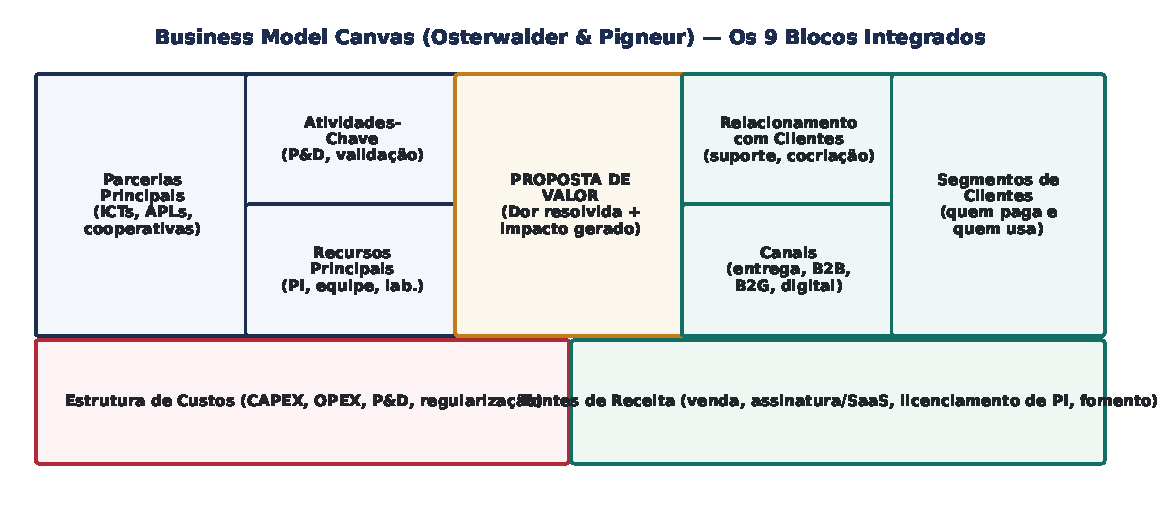
\includegraphics[width=0.95\textwidth]{figures/fig09_canvas_lean.pdf}
  \caption{Arquitetura integrada do \textit{Business Model Canvas}, ajuste Proposta de Valor–Cliente e ciclo \textit{Lean Startup} (Construir–Medir–Aprender).}
  \label{fig:09_canvas_lean}
\end{figure}

\begin{boxFormula}[Métricas Unitárias: CAC, LTV, Razão LTV/CAC e \textit{Payback} do CAC]
  \textbf{1. Custo de Aquisição de Cliente (CAC):} mede quanto custa, em média, conquistar um novo cliente pagante em determinado período:
  \[
    \text{CAC} = \frac{\text{Despesas de Marketing} + \text{Despesas de Vendas}}{\text{Número de Novos Clientes Adquiridos no Período}}.
  \]

  \textbf{2. Valor do Tempo de Vida do Cliente (LTV, \textit{Lifetime Value}):} mede a margem bruta total gerada por um cliente antes de cancelar o serviço. Sendo $\text{ARPU}$ o ticket médio mensal, $m$ a margem bruta percentual (em decimal) e $\delta$ a taxa mensal de cancelamento (\textit{churn}), o tempo médio de retenção é $\bar{T} = \frac{1}{\delta}$ meses, resultando em:
  \[
    \text{MC}_{\text{mensal}} = \text{ARPU} \times m, \qquad
    \text{LTV} = \text{MC}_{\text{mensal}} \times \bar{T} = \frac{\text{ARPU} \times m}{\delta}.
  \]

  \textbf{3. Razão LTV/CAC e Tempo de Retorno (\textit{Payback}) do CAC:}
  \[
    \text{Razão } \frac{\text{LTV}}{\text{CAC}} \ge 3{,}0 \text{ (referência saudável)}, \qquad
    \text{Payback}_{\text{CAC}} = \frac{\text{CAC}}{\text{MC}_{\text{mensal}}} \text{ (em meses)}.
  \]
  Se $\text{LTV}/\text{CAC} < 1$, a empresa destrói valor a cada novo cliente adquirido; entre $1$ e $3$, a margem para cobrir custos fixos de P\&D e estrutura é estreita; acima de $3$, o motor comercial sustenta crescimento com retorno sobre o capital investido em vendas.
\end{boxFormula}

\etapa{4}{Estudos de Caso e Exemplos Resolvidos em 7 Passos}

\begin{boxExemplo}{9.1}{Cálculo de CAC, LTV, Razão LTV/CAC e \textit{Payback} em SaaS Agrícola}
  \passoEnunciado{Uma agtech sediada em Juazeiro (BA) comercializa um software de manejo de irrigação por assinatura mensal para produtores de fruticultura.}
  \passoDados{Despesas mensais de marketing digital e feiras locais: R\$\,9.000,00. Despesas mensais com equipe de vendas técnicas (salários, comissões e deslocamento): R\$\,15.000,00. Novos clientes pagantes conquistados no mês: 20 produtores. Ticket médio mensal ($\text{ARPU}$): R\$\,450,00. Margem bruta operacional ($m$): 80\% ($0{,}80$). Taxa mensal de cancelamento (\textit{churn}, $\delta$): 4\% ($0{,}04$).}
  \passoPedido{Calcular o CAC, a margem de contribuição mensal por cliente, o tempo médio de retenção, o LTV, a razão LTV/CAC e o \textit{payback} do CAC.}
  \passoMetodo{Aplicação direta das equações unitárias de economia de assinaturas (SaaS).}
  \passoContas{
    Primeiro, calcula-se o CAC:
    \[
      \text{CAC} = \frac{9.000,00 + 15.000,00}{20} = \frac{24.000,00}{20} = \text{R\$\,1.200,00}.
    \]
    Em seguida, obtém-se a margem de contribuição mensal por cliente e o tempo médio de retenção:
    \[
      \text{MC}_{\text{mensal}} = 450,00 \times 0{,}80 = \text{R\$\,360,00/mês}, \qquad
      \bar{T} = \frac{1}{0{,}04} = 25\text{ meses}.
    \]
    Multiplicando a margem mensal pela permanência média, encontra-se o LTV:
    \[
      \text{LTV} = 360,00 \times 25 = \text{R\$\,9.000,00}.
    \]
    Por fim, avaliam-se a razão LTV/CAC e o \textit{payback} do CAC:
    \[
      \frac{\text{LTV}}{\text{CAC}} = \frac{9.000,00}{1.200,00} = 7{,}50, \qquad
      \text{Payback}_{\text{CAC}} = \frac{1.200,00}{360,00} = 3{,}33\text{ meses}.
    \]
  }
  \passoResposta{$\text{CAC} = \text{R\$\,1.200,00}$; $\text{LTV} = \text{R\$\,9.000,00}$; $\text{LTV/CAC} = 7{,}50$; \textit{payback} do CAC $= 3{,}33\text{ meses}$.}
  \passoVerificacao{Uma razão de 7{,}50 (muito acima do piso de 3{,}0) com recuperação do custo de venda em pouco mais de três meses indica forte sustentabilidade unitária para escalar a equipe comercial.}
\end{boxExemplo}

\begin{boxExemplo}{9.2}{Arquitetura do \textit{Business Model Canvas} para Rastreabilidade do Leite}
  \passoEnunciado{Uma equipe técnica propõe implantar um sistema de sensores térmicos e aplicativo de controle de qualidade do leite para cooperativas da bacia leiteira do Portal do Sertão.}
  \passoDados{Os produtores individuais têm baixa margem e resistência a mensalidades, mas os laticínios e cooperativas perdem em média 8\% do volume coletado por acidificação e pagam bônus por baixa contagem bacteriana.}
  \passoPedido{Estruturar o ajuste Proposta de Valor–Segmento de Clientes e definir os blocos críticos de Receita, Canais e Parcerias do BMC.}
  \passoMetodo{Modelagem nos nove blocos do BMC de Osterwalder e Pigneur (2010), distinguindo usuário de campo e pagador.}
  \passoContas{
    Se o modelo cobrasse dos produtores isolados, o CAC seria elevado e a conversão baixa. Ao reposicionar o \textbf{Segmento de Clientes} pagante para as cooperativas/laticínios (modelo B2B2C), a \textbf{Proposta de Valor} passa a ser a redução de descarte de leite contaminado e a elevação do preço pago por qualidade superior. Os \textbf{Canais} e \textbf{Parcerias} utilizam os próprios caminhões de coleta e técnicos de assistência rural já existentes na cooperativa, reduzindo drasticamente o custo de distribuição. A \textbf{Fonte de Receita} torna-se assinatura mensal por tanque resfriador monitorado paga pela cooperativa.
  }
  \passoResposta{Modelo B2B2C: o produtor usa o aplicativo sem custo direto; a cooperativa/laticínio paga pela assinatura por tanque monitorado em troca da redução de perdas de matéria-prima.}
  \passoVerificacao{O ajuste resolve a assimetria de capacidade de pagamento do território sem sacrificar a capilaridade de coleta de dados.}
\end{boxExemplo}

\begin{boxExemplo}{9.3}{Métricas de Vaidade vs. Métricas Acionáveis no Ciclo \textit{Lean}}
  \passoEnunciado{Um aplicativo de comercialização direta para agricultores familiares acumulou 12.000 downloads após campanha em redes sociais com gasto de R\$\,1.200,00, mas apenas 180 usuários realizaram compras recorrentes.}
  \passoDados{Investimento em mídia = R\$\,1.200,00. Downloads totais = 12.000. Compradores recorrentes antes do ajuste = 180 (taxa de conversão de download para comprador recorrente = $1{,}5\%$). Após redesenho do fluxo de cadastro (MVP 2) com o mesmo gasto de R\$\,1.200,00, os downloads foram 1.500, porém a conversão subiu para $20\%$ ($300$ compradores recorrentes).}
  \passoPedido{Identificar a métrica de vaidade e calcular o CAC efetivo por comprador recorrente antes e depois do ciclo Construir–Medir–Aprender.}
  \passoMetodo{Diferenciação entre volume bruto de exposição e custo efetivo de aquisição de usuário ativo pagante.}
  \passoContas{
    O número de downloads (12.000) é uma \textbf{métrica de vaidade}, pois mascara o abandono de $98{,}5\%$ dos usuários. Calculando o CAC efetivo por comprador recorrente:
    \[
      \text{CAC}_{\text{antes}} = \frac{1.200,00}{180} \approx \text{R\$\,6{,}67/comprador}, \qquad
      \text{CAC}_{\text{depois}} = \frac{1.200,00}{300} = \text{R\$\,4{,}00/comprador}.
    \]
    Apesar de os downloads caírem de 12.000 para 1.500, o CAC efetivo foi reduzido em $(6{,}67 - 4{,}00)/6{,}67 \approx 40{,}0\%$.
  }
  \passoResposta{Downloads constituem métrica de vaidade; o ciclo \textit{Lean} aumentou os compradores recorrentes de 180 para 300 e reduziu o CAC efetivo de R\$\,6{,}67 para R\$\,4{,}00.}
  \passoVerificacao{O exemplo ilustra por que decisões orientadas por métricas acionáveis evitam investir em divulgação antes de corrigir gargalos de ativação no MVP.}
\end{boxExemplo}

\begin{boxExemplo}{9.4}{Pivô de Modelo de Receita: Venda de Equipamento para HaaS}
  \passoEnunciado{Uma startup desenvolveu estações meteorológicas automatizadas para prefeituras e consórcios municipais. No modelo original, tentava vender cada estação por R\$\,24.000,00 à vista (CAPEX do cliente), mas esbarrava em processos licitatórios lentos e falta de manutenção local.}
  \passoDados{Custo de fabricação de cada estação: R\$\,9.000,00. Custo mensal de manutenção e conectividade: R\$\,120,00/estação. Novo modelo proposto (\textit{Hardware as a Service}, HaaS): assinatura de R\$\,920,00/mês em contrato de 36 meses, sem custo inicial de aquisição para o município.}
  \passoPedido{Calcular a margem de contribuição mensal líquida da manutenção e em quantos meses a startup recupera o custo de fabricação da estação no modelo HaaS.}
  \passoMetodo{Análise de transição CAPEX para OPEX e cálculo de \textit{payback} do equipamento.}
  \passoContas{
    Receita líquida mensal após custos recorrentes de conectividade/manutenção:
    \[
      \text{Saldo mensal por estação} = 920,00 - 120,00 = \text{R\$\,800,00/mês}.
    \]
    Tempo necessário para recuperar o custo de fabricação (R\$\,9.000,00):
    \[
      \text{Payback do hardware} = \frac{9.000,00}{800,00} = 11{,}25\text{ meses}.
    \]
    Ao longo do contrato de 36 meses, o fluxo líquido por estação após pagar o hardware será $36 \times 800,00 - 9.000,00 = 28.800,00 - 9.000,00 = \text{R\$\,19.800,00}$.
  }
  \passoResposta{O custo de fabricação é recuperado em 11{,}25 meses, gerando saldo líquido de R\$\,19.800,00 por estação ao longo de 36 meses.}
  \passoVerificacao{O pivô elimina a barreira de entrada orçamentária do cliente, mas exige da startup capital de giro para financiar os primeiros 11{,}25 meses de fabricação.}
\end{boxExemplo}

\begin{boxExemplo}{9.5}{Mediação Tecnológica e Captura de Valor (Chesbrough \& Rosenbloom)}
  \passoEnunciado{Um grupo universitário desenvolveu uma membrana filtrante cerâmica 30\% mais durável que as membranas poliméricas importadas usadas em pequenas queijarias artesanais.}
  \passoDados{A membrana importada custa R\$\,400,00 e dura 6 meses. A membrana cerâmica universitária tem custo de produção de R\$\,600,00 e dura 18 meses, mas exige um suporte de aço inox que custa R\$\,1.200,00 na primeira compra.}
  \passoPedido{Explicar por que tentar vender o conjunto inicial a R\$\,1.800,00 à vista fracassa junto às pequenas queijarias e propor uma reconfiguração de modelo de negócio.}
  \passoMetodo{Comparação de desembolso inicial vs. custo total de propriedade (TCO) e arquitetura de captura de valor.}
  \passoContas{
    Em 18 meses, a queijaria gastaria $3 \times 400,00 = \text{R\$\,1.200,00}$ com a membrana importada (desembolso parcelado de R\$\,400,00 a cada semestre). Embora a cerâmica seja tecnicamente superior, cobrar R\$\,1.800,00 à vista na entrada representa 4{,}5 vezes o desembolso semestral habitual do produtor. Se a startup mantiver a propriedade do suporte de aço inox em comodato e cobrar apenas R\$\,70,00/mês pelo serviço de filtração com reposição garantida, o gasto em 18 meses será $18 \times 70,00 = \text{R\$\,1.260,00}$ (praticamente igual ao importado), diluindo a barreira inicial e gerando receita previsível.
  }
  \passoResposta{A tecnologia fracassa no modelo de venda direta por causa da barreira de entrada de R\$\,1.800,00; o modelo de comodato com assinatura mensal destrava a adoção.}
  \passoVerificacao{O caso confirma a tese de Chesbrough e Rosenbloom (2002): a inovação está tanto no modelo de cobrança e relacionamento quanto no material cerâmico.}
\end{boxExemplo}

\etapa{5}{Armadilhas Conceituais e Erros Mais Comuns}

\begin{boxErro}[Erro 1: Preencher o \textit{Business Model Canvas} como Documento Estático]
  Muitos estudantes tratam o preenchimento dos nove quadros do BMC como o encerramento do planejamento. Na prática, um Canvas inicial é apenas um conjunto de hipóteses não verificadas; cada bloco precisa ser testado em campo e revisado à medida que entrevistas e MVPs revelam o comportamento real dos clientes.
\end{boxErro}

\begin{boxErro}[Erro 2: Calcular o LTV Sobre o Faturamento Bruto em Vez da Margem Bruta]
  Multiplicar o ticket médio pelo tempo de retenção sem aplicar a margem bruta ($m$) superestima gravemente o LTV. Em empresas com custos variáveis elevados (hardware, insumos físicos, taxas de pagamento), usar a receita bruta no numerador mascara um negócio deficitário como se tivesse boa relação LTV/CAC.
\end{boxErro}

\begin{boxErro}[Erro 3: Tratar o MVP como Produto Mal Acabado ou Defeituoso]
  Construir um MVP não significa entregar uma solução tecnicamente insegura ou inoperante ao cliente. Significa reduzir o escopo funcional ao núcleo mínimo necessário para validar a proposta de valor principal, preservando confiabilidade técnica no atributo testado.
\end{boxErro}

\begin{boxErro}[Erro 4: Subestimar Custos Comerciais no Cálculo do CAC]
  Computar apenas anúncios digitais no numerador do CAC e omitir salários de vendedores, viagens técnicas no território, comissões e tempo gasto em demonstrações distorce o indicador para baixo e compromete a projeção de capital de giro.
\end{boxErro}

\etapa{6}{Lista de Exercícios (15 Questões em 3 Níveis)}

\textbf{Nível 1, Fundamentos Conceituais (Questões 1 a 5)}

\begin{enumerate}[leftmargin=1.5em, itemsep=6pt]
  \item Explique a tese de Chesbrough e Rosenbloom (2002) sobre o papel mediador do modelo de negócio entre tecnologia e geração de valor econômico.
  \espacoResolucao[1.8cm]

  \item Liste os nove blocos do \textit{Business Model Canvas} e explique a diferença lógica entre os blocos do lado direito (valor/mercado) e os do lado esquerdo (eficiência/infraestrutura).
  \espacoResolucao[1.8cm]

  \item Diferencie as quatro etapas do \textit{Customer Development} de Steve Blank e explique por que elas antecedem a contratação de uma grande equipe de vendas.
  \espacoResolucao[1.8cm]

  \item Descreva o ciclo Construir–Medir–Aprender de Eric Ries e dê dois exemplos de métricas de vaidade e dois de métricas acionáveis para uma plataforma territorial.
  \espacoResolucao[1.8cm]

  \item Qual a diferença conceitual entre ajustar parâmetros de preço e realizar um pivô no modelo de negócio?
  \espacoResolucao[1.8cm]

  \item \textbf{(Nível 2, Aplicações Numéricas)} Uma startup investiu R\$\,18.000,00 em marketing e R\$\,27.000,00 em vendas em um trimestre, conquistando 30 novos clientes corporativos. Calcule o CAC desse período.
  \espacoResolucao[2.1cm]

  \item Um serviço de monitoramento de silos agrícolas cobra mensalidade de R\$\,600,00, apresenta margem bruta de 75\% e taxa de cancelamento (\textit{churn}) de 5\% ao mês. Calcule a margem de contribuição mensal por cliente, o tempo médio de retenção e o LTV.
  \espacoResolucao[2.2cm]

  \item Utilizando o LTV obtido no exercício anterior e considerando um $\text{CAC} = \text{R\$\,2.250,00}$, calcule a razão $\text{LTV/CAC}$ e o \textit{payback} do CAC em meses. O resultado atende ao padrão saudável do mercado?
  \espacoResolucao[2.2cm]

  \item Uma empresa tem $\text{ARPU} = \text{R\$\,200,00}$, margem bruta de 60\% e deseja manter a razão $\text{LTV/CAC} = 4{,}0$. Se o CAC atual é de R\$\,1.200,00, qual deve ser a taxa máxima mensal de \textit{churn} ($\delta$) tolerável?
  \espacoResolucao[2.3cm]

  \item Um marketplace regional gasta R\$\,4.000,00 por mês em aquisição digital. No Mês 1 obteve 2.000 cadastros gratuitos e apenas 40 vendedores ativos pagantes. No Mês 2, após simplificar o MVP, obteve 800 cadastros e 100 vendedores ativos pagantes. Calcule a variação percentual do CAC efetivo por vendedor ativo pagante.
  \espacoResolucao[2.3cm]

  \item \textbf{(Nível 3, Análise Territorial e Estratégica)} Uma cooperativa de apicultura pretende adotar um software de rastreabilidade. Estruture os nove blocos do BMC indicando explicitamente quem é o usuário de campo, quem é o pagador e quais parcerias territoriais reduzem o CAC.
  \espacoResolucao[2.3cm]

  \item Uma startup vende sensores de solo com $\text{CAC} = \text{R\$\,3.000,00}$, $\text{ARPU} = \text{R\$\,500,00}$, margem bruta $= 50\%$ e \textit{churn} $= 10\%$ ao mês. Demonstre numericamente por que escalar investimentos em vendas nessa configuração destruiria ou comprometeria o capital da empresa e proponha duas alavancas corretivas.
  \espacoResolucao[2.4cm]

  \item Explique como o uso de cooperativas, sindicatos rurais ou associações comerciais como **Canais** e **Parcerias Principais** no BMC altera simultaneamente o CAC e o tempo de retenção (LTV) em territórios interioranos.
  \espacoResolucao[2.2cm]

  \item Uma empresa vende um software agrícola com contrato anual pago à vista de R\$\,4.800,00 (equivalente a R\$\,400,00/mês) e margem bruta de 85\%. Se o \textit{churn} anualizado corresponder a uma permanência média de 30 meses e o CAC for de R\$\,2.040,00, calcule o LTV, a razão LTV/CAC e explique a vantagem financeira da cobrança anual antecipada sobre o fluxo de caixa.
  \espacoResolucao[2.4cm]

  \item Desenhe um protocolo de MVP de baixo custo (sem programação pesada) para validar a disposição a pagar de pequenas agroindústrias baianas por um serviço de certificação energética e rastreabilidade ambiental.
  \espacoResolucao[2.3cm]
\end{enumerate}

\etapa{7}{Questões Autorais Estilo Pós-Graduação / Concursos de CT\&I}

\begin{enumerate}[leftmargin=1.5em, itemsep=6pt]
  \item \textbf{(Estilo ANPAD / Estratégia e Inovação)} Sobre o ciclo \textit{Lean Startup} e a economia unitária de modelos de negócio, analise as afirmações:
  I. O LTV deve ser calculado considerando a margem bruta gerada pelo cliente ao longo do seu tempo de retenção, e não apenas o faturamento bruto, sob pena de superestimar a viabilidade de aquisição.
  II. Um elevado volume de downloads gratuitos ou seguidores em redes sociais caracteriza uma métrica acionável suficiente para validar o \textit{Product-Market Fit}.
  III. Em mercados territoriais pulverizados, parcerias institucionais com cooperativas e associações podem reduzir o CAC ao concentrar múltiplos usuários em um único canal de venda.
  Assinale a alternativa correta:
  \begin{alternativas}
    \item Apenas I está correta.
    \item Apenas II está correta.
    \item Apenas I e III estão corretas.
    \item Apenas II e III estão corretas.
    \item I, II e III estão corretas.
  \end{alternativas}
  \espacoResolucao[1.5cm]

  \item \textbf{(Estilo Concurso Analista de Projetos / Gestão)} Uma empresa de serviços digitais para gestão hídrica possui ticket médio mensal de R\$\,500,00, margem bruta de 70\%, \textit{churn} mensal de 2{,}5\% e CAC de R\$\,3.500,00. Assinale a alternativa que apresenta corretamente o LTV, a razão LTV/CAC e o \textit{payback} do CAC:
  \begin{alternativas}
    \item $\text{LTV} = \text{R\$\,14.000,00}$; $\text{LTV/CAC} = 4{,}0$; $\text{Payback} = 10{,}0\text{ meses}$.
    \item $\text{LTV} = \text{R\$\,20.000,00}$; $\text{LTV/CAC} = 5{,}7$; $\text{Payback} = 7{,}0\text{ meses}$.
    \item $\text{LTV} = \text{R\$\,14.000,00}$; $\text{LTV/CAC} = 4{,}0$; $\text{Payback} = 7{,}0\text{ meses}$.
    \item $\text{LTV} = \text{R\$\,10.500,00}$; $\text{LTV/CAC} = 3{,}0$; $\text{Payback} = 10{,}0\text{ meses}$.
    \item $\text{LTV} = \text{R\$\,17.500,00}$; $\text{LTV/CAC} = 5{,}0$; $\text{Payback} = 10{,}0\text{ meses}$.
  \end{alternativas}
  \espacoResolucao[1.6cm]

  \item \textbf{(Estilo Discursiva, PPGPT)} Um laboratório universitário desenvolveu um método eficiente para transformar resíduos de cacau em embalagem biodegradável, porém nenhuma indústria regional adquiriu o processo quando ofertado via venda direta de patente. Com base em Chesbrough \& Rosenbloom (2002) e Osterwalder \& Pigneur (2010), explique por que a excelência técnica falhou em gerar adoção e proponha uma reformulação de modelo de negócio.
  \espacoResolucao[2.4cm]
\end{enumerate}

\begin{boxDica}[Contraponto Crítico e Prática Territorial (AV3)]
  No Projeto Final (AV3), apresente o \textit{Business Model Canvas} completo do seu empreendimento ou arranjo territorial, mas não se limite a preencher os nove quadros: explicite qual é a hipótese mais arriscada do Canvas, qual MVP foi ou será usado para testá-la e calcule explicitamente o CAC e o LTV esperados.
\end{boxDica}

\clearpage
\etapa{8}{Gabarito Integralmente Comentado (Exercícios 1 a 18)}

\begin{boxGabarito}[Resolução Completa dos Exercícios da Etapa 6 (1 a 15) e Etapa 7 (16 a 18)]
  \begin{enumerate}[leftmargin=1.5em, itemsep=4pt]
    \item \textbf{Resposta:} Segundo Chesbrough e Rosenbloom (2002), a tecnologia possui apenas valor latente; o modelo de negócio funciona como mediador cognitivo e econômico que define proposta de valor, segmento, cadeia produtiva e mecanismo de captura de receita.
    \item \textbf{Resposta:} Os 9 blocos são: Segmentos de Clientes, Proposta de Valor, Canais, Relacionamento, Fontes de Receita (eixo de valor/mercado, lado direito); Recursos Principais, Atividades-Chave, Parcerias Principais e Estrutura de Custos (eixo de eficiência/infraestrutura, lado esquerdo).
    \item \textbf{Resposta:} Descoberta do cliente, Validação do cliente, Criação de demanda e Construção da empresa. As duas primeiras etapas verificam se há dor real e disposição a pagar antes de investir pesado em força comercial.
    \item \textbf{Resposta:} Construir (MVP) $\to$ Medir (comportamento real) $\to$ Aprender (perseverar ou pivotar). Vaidade: curtidas e downloads brutos. Acionáveis: taxa de ativação pagante, retenção mensal e CAC.
    \item \textbf{Resposta:} Ajustar preço é uma otimização tática dentro da mesma hipótese de negócio; pivotar é mudar estruturalmente um ou mais pilares do modelo (segmento, proposta de valor, canal ou forma de monetização).
    \item \textbf{Resposta:} $\text{CAC} = (18.000 + 27.000) / 30 = 45.000 / 30 = \text{R\$\,1.500,00}$.
    \item \textbf{Resposta:} $\text{MC}_{\text{mensal}} = 600 \times 0{,}75 = \text{R\$\,450,00/mês}$. Retenção média $= 1 / 0{,}05 = 20\text{ meses}$. $\text{LTV} = 450 \times 20 = \text{R\$\,9.000,00}$.
    \item \textbf{Resposta:} $\text{LTV/CAC} = 9.000 / 2.250 = 4{,}0$. $\text{Payback}_{\text{CAC}} = 2.250 / 450 = 5{,}0\text{ meses}$. Sim, atende ao padrão saudável ($\text{LTV/CAC} \ge 3{,}0$).
    \item \textbf{Resposta:} $\text{MC}_{\text{mensal}} = 200 \times 0{,}60 = \text{R\$\,120,00}$. Para $\text{LTV/CAC} = 4{,}0$, exige-se $\text{LTV} = 4 \times 1.200 = \text{R\$\,4.800,00}$. Como $\text{LTV} = \text{MC}_{\text{mensal}} / \delta$, tem-se $\delta = 120 / 4.800 = 0{,}025 = 2{,}5\%$ ao mês.
    \item \textbf{Resposta:} $\text{CAC}_{\text{M1}} = 4.000 / 40 = \text{R\$\,100,00}$. $\text{CAC}_{\text{M2}} = 4.000 / 100 = \text{R\$\,40,00}$. Redução de $(100 - 40)/100 = 60\%$.
    \item \textbf{Resposta:} Usuário: apicultor cooperado; Pagador: cooperativa ou entreposto exportador; Parcerias: cooperativas, SENAR/SEBRAE e ICTs; Canais: técnicos de campo da cooperativa, reduzindo drasticamente o CAC unitário.
    \item \textbf{Resposta:} $\text{MC}_{\text{mensal}} = 500 \times 0{,}50 = \text{R\$\,250,00}$. Retenção $= 1 / 0{,}10 = 10\text{ meses}$. $\text{LTV} = 250 \times 10 = \text{R\$\,2.500,00}$. Como $\text{CAC} = \text{R\$\,3.000,00}$, $\text{LTV/CAC} = 2.500 / 3.000 \approx 0{,}83 < 1{,}0$ e o \textit{payback} ($3.000 / 250 = 12\text{ meses}$) supera a permanência média (10 meses), destruindo R\$\,500,00 por cliente. Alavancas: reduzir o CAC via vendas em grupo (cooperativas) e reduzir o \textit{churn} com suporte pós-venda.
    \item \textbf{Resposta:} Vender via cooperativas dilui o esforço de prospecção em dezenas de produtores por contrato (reduzindo o CAC) e ancora o uso da solução na rotina coletiva (reduzindo o \textit{churn} e elevando o LTV).
    \item \textbf{Resposta:} $\text{MC}_{\text{mensal}} = 400 \times 0{,}85 = \text{R\$\,340,00}$. $\text{LTV} = 340 \times 30 = \text{R\$\,10.200,00}$. $\text{LTV/CAC} = 10.200 / 2.040 = 5{,}0$. A cobrança anual antecipada (R\$\,4.800,00 no ato) cobre imediatamente o CAC de R\$\,2.040,00, financiando o crescimento sem depender de capital de giro externo.
    \item \textbf{Resposta:} MVP tipo *concierge* ou página de pré-reserva: apresentar um dossiê demonstrativo a 10 agroindústrias com simulação personalizada de economia energética e solicitar carta de intenção ou pagamento simbólico de diagnóstico piloto antes de desenvolver a plataforma automatizada.
    \item \textbf{Questão 16 (Etapa 7), Gabarito: (C).} II é falsa porque downloads gratuitos e seguidores são métricas de vaidade.
    \item \textbf{Questão 17 (Etapa 7), Gabarito: (A).} $\text{MC}_{\text{mensal}} = 500 \times 0{,}70 = \text{R\$\,350,00}$; Retenção $= 1 / 0{,}025 = 40\text{ meses}$; $\text{LTV} = 350 \times 40 = \text{R\$\,14.000,00}$; $\text{LTV/CAC} = 14.000 / 3.500 = 4{,}0$; $\text{Payback} = 3.500 / 350 = 10{,}0\text{ meses}$.
    \item \textbf{Questão 18 (Etapa 7), Espelho Discursivo:} Deve explicar que a venda direta de patente transfere todo o risco tecnológico e de escala para indústrias locais que não têm P\&D interna. A reformulação propõe ofertar a embalagem pronta (via parceria com convertedor local ou produção sob contrato) ou licenciamento escalonado por volume com validação piloto compartilhada.
  \end{enumerate}
\end{boxGabarito}

\begin{boxResumo}
  \begin{itemize}[leftmargin=1.4em, itemsep=2pt]
    \item O modelo de negócio traduz potencial técnico em captura econômica de valor.
    \item O \textit{Business Model Canvas} integra mercado (lado direito) e operação (lado esquerdo) a partir do ajuste Proposta de Valor–Segmento de Clientes.
    \item O ciclo Construir–Medir–Aprender via MVPs substitui suposições por métricas acionáveis: $\text{LTV/CAC} \ge 3{,}0$ e \textit{payback} do CAC inferior ao tempo de retenção.
  \end{itemize}
\end{boxResumo}

\begin{boxTeste}
  \begin{enumerate}[leftmargin=1.5em, itemsep=4pt]
    \item (\V/\F) Segundo Chesbrough e Rosenbloom (2002), uma tecnologia superior captura valor automaticamente no mercado, independentemente do modelo de negócio adotado.
    \item (\V/\F) No cálculo do LTV, deve-se multiplicar a receita mensal pela margem bruta antes de dividir pela taxa mensal de \textit{churn}.
    \item (\V/\F) Se $\text{CAC} = \text{R\$\,1.000,00}$, $\text{ARPU} = \text{R\$\,250,00}$, margem bruta $= 80\%$ e \textit{churn} $= 5\%$ ao mês, então $\text{LTV} = \text{R\$\,4.000,00}$ e $\text{LTV/CAC} = 4{,}0$.
    \item (\V/\F) O total de curtidas e visualizações em redes sociais é exemplo clássico de métrica acionável para comprovar validação de modelo de negócio.
  \end{enumerate}
  \begin{boxGabarito}[Respostas do Checkpoint: Capítulo 9]
    \textbf{1: \F} (O modelo de negócio é o mediador indispensável). \quad \textbf{2: \V}. \quad \textbf{3: \V} ($\text{MC} = 200$; Retenção $= 20$; $\text{LTV} = 4.000$; $\text{LTV/CAC} = 4{,}0$). \quad \textbf{4: \F} (Trata-se de métrica de vaidade).
  \end{boxGabarito}
\end{boxTeste}

\chapter{Planos de Negócio e Instrumentos de Fomento Regional}
\label{cap:10}
\markboth{CAPÍTULO 10 — PLANOS DE NEGÓCIO E FOMENTO}{CAPÍTULO 10 — PLANOS DE NEGÓCIO E FOMENTO}

\noindent\tagTerritorio\ \tagAV{Base AV3}

\begin{capObjetivos}
  Ao concluir este capítulo, você será capaz de:
  \begin{enumerate}[leftmargin=1.5em, itemsep=2pt]
    \item Diferenciar a função contemporânea do Plano de Negócio completo, do Sumário Executivo e do \textit{Pitch Deck} conforme o interlocutor e o estágio do empreendimento.
    \item Mapear a \textbf{Escada do Capital} para Empreendimentos de Base Tecnológica (EBT), distinguindo recursos não dilutivos de capital societário (\textit{equity}) e crédito subsidiado.
    \item Identificar os principais instrumentos brasileiros e regionais de fomento à inovação (CNPq, FAPESB, FINEP, Programa Centelha, BNB/FNE Inovação e BNDES).
    \item Calcular indicadores de tração e fôlego financeiro: \textbf{MRR, \textit{Gross Burn Rate}, \textit{Net Burn Rate}, \textit{Runway}} em meses e prazo até o ponto de equilíbrio operacional.
  \end{enumerate}
\end{capObjetivos}

\begin{capRevisao}
  Recupere três elementos estruturantes dos capítulos anteriores:
  \begin{itemize}[leftmargin=1.5em, itemsep=2pt]
    \item \textbf{Vale da Morte Tecnológico (Cap. 7):} o intervalo entre TRL 4 e TRL 6 exige capital paciente capaz de suportar fluxos de caixa acumulados negativos antes da escala comercial.
    \item \textbf{Dimensionamento TAM/SAM/SOM (Cap. 8):} agências de fomento e investidores avaliam a coerência entre o montante solicitado e o mercado alcançável (\textit{bottom-up}).
    \item \textbf{Economia Unitária (Cap. 9):} antes de buscar capital de risco ou crédito de expansão, a empresa precisa demonstrar validação do MVP e relação $\text{LTV/CAC} \ge 3{,}0$.
  \end{itemize}
\end{capRevisao}

\etapa{3}{Explicação Teórica, Vocabulário Prévio e Modelos}

\begin{boxSimbolo}[Vocabulário Conceitual e Símbolos do Capítulo 10]
  \begin{tabularx}{\textwidth}{@{}l >{\raggedright\arraybackslash}X@{}}
    \textbf{MRR} & \textit{Monthly Recurring Revenue} — receita recorrente mensal contratada pela base ativa de clientes. \\
    \textbf{\textit{Gross Burn}} & Queima bruta de caixa: soma de todas as despesas operacionais mensais da empresa. \\
    \textbf{\textit{Net Burn}} & Queima líquida mensal de caixa ($\text{Despesas Operacionais} - \text{Receita Mensal}$). \\
    \textbf{\textit{Runway}} & Fôlego financeiro em meses: tempo até o caixa disponível zerar caso o \textit{Net Burn} atual permaneça constante. \\
    \textbf{Não Dilutivo} & Capital captado sem cessão de participação societária (subvenção econômica, bolsas, premiações). \\
    \textbf{\textit{Equity} / Diluição} & Capital investido em troca de percentual societário da empresa (anjo, \textit{seed}, \textit{Venture Capital}). \\
  \end{tabularx}
\end{boxSimbolo}

\section{Para que Serve o Plano de Negócio Hoje?}

Durante muito tempo, o ensino tradicional de empreendedorismo exigia que fundadores redigissem planos de negócio extensos (60 a 100 páginas) antes mesmo de conversar com um único cliente. O avanço das abordagens \textit{Effectuation} e \textit{Lean Startup} evidenciou que planos rígidos elaborados sem validação empírica tornam-se obsoletos no primeiro contato com o mercado. Contudo, isso não significa que o planejamento formal perdeu utilidade; sua função deslocou-se da etapa de descoberta inicial para a etapa de **alinhamento estratégico, captação de fomento e governança**.

Atualmente, três formatos coexistem com finalidades distintas:
\begin{itemize}[leftmargin=1.5em, itemsep=2pt]
  \item \textbf{\textit{Pitch Deck} (10 a 15 slides):} apresentação visual concisa usada para despertar interesse inicial de investidores-anjo, aceleradoras e bancas de programas como o Centelha. Sintetiza problema, solução, tamanho de mercado (TAM/SAM/SOM), modelo de negócio, tração atual, equipe e necessidade de capital.
  \item \textbf{Sumário Executivo (2 a 4 páginas):} documento textual objetivo voltado à triagem em editais de subvenção, parques tecnológicos e comitês de crédito, reunindo tese técnica, diferencial de PI, orçamento macro e metas de entrega.
  \item \textbf{Plano de Negócio Completo:} documento analítico detalhado exigido para aprovações de crédito regional (BNB/FNE, BNDES), rodadas estruturadas de \textit{Venture Capital}, projetos industriais ou articulações institucionais complexas (como o Projeto Final AV3). Contém análise locacional, engenharia de custos (CAPEX/OPEX) e projeções financeiras completas.
\end{itemize}

\section{A Escada do Capital para EBTs e o Fomento Regional}

Financiar uma empresa de base tecnológica com o instrumento errado no momento errado destrói valor. Tomar empréstimo bancário com juros comerciais em TRL 3 gera insolvência antes da primeira venda; inversamente, ceder 30\% da empresa a investidores privados para financiar pesquisa básica que poderia ser coberta por subvenção pública gera diluição desnecessária. A **Escada do Capital** organiza as fontes financeiras em sequência compatível com a maturidade tecnológica (TRL) e o risco do negócio:

\begin{enumerate}[leftmargin=1.5em, itemsep=2pt]
  \item \textbf{\textit{Bootstrapping} e FFF (\textit{Family, Friends and Fools}):} uso de recursos próprios dos fundadores, serviços de consultoria paralela ou pequenas contribuições de rede próxima para construir protótipos iniciais (TRL 2–4) sem diluição externa.
  \item \textbf{Subvenção Econômica e Fomento Não Reembolsável:} recursos públicos destinados a compartilhar o risco tecnológico em empresas nascentes sem exigir devolução financeira nem participação societária. Destacam-se o **CNPq** (bolsas RHAE e editais de pesquisa aplicada), as fundações estaduais como a **FAPESB** na Bahia (editais de inovação e *startups*), o **Programa Centelha** (FINEP/CNPq/FAPs para ideias inovadoras) e os editais **FINEP** (Tecnova, Subvenção Econômica e FINEP Startup).
  \item \textbf{Investidor-Anjo e Redes de Investidores:} pessoas físicas experientes que aportam capital próprio (tipicamente entre R\$\,100 mil e R\$\,1 milhão) somado a mentoria e rede de contatos (\textit{smart money}) via contratos de mútuo conversível ou participação societária minoritária, apoiando a validação comercial (TRL 5–7).
  \item \textbf{\textit{Venture Capital} (Seed e Série A):} fundos institucionais que investem capital de terceiros em empresas com modelo validado e tração comprovada (TRL 7–9) visando crescimento acelerado e saída futura.
  \item \textbf{Crédito Regional e de Fomento Industrial:} financiamentos reembolsáveis com taxas e prazos diferenciados para implantação fabril, capital de giro e expansão territorial. No Nordeste e na Bahia, destaca-se o **Banco do Nordeste (BNB)** por meio do **FNE Inovação** (com prazos longos e carência compatível com maturação de projetos), além das linhas do **BNDES** (BNDES Finem, BNDES Inovação) e agências estaduais como a Desenbahia.
\end{enumerate}

\begin{figure}[H]
  \centering
  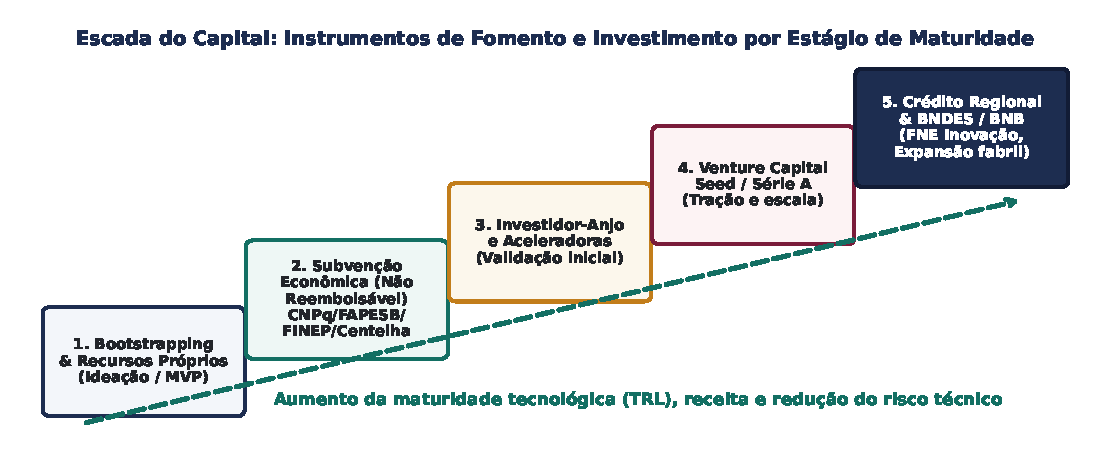
\includegraphics[width=0.94\textwidth]{figures/fig10_escada_capital.pdf}
  \caption{Escada do Capital para Empreendimentos de Base Tecnológica: alinhamento entre estágio TRL, instrumentos de fomento regional e diluição societária.}
  \label{fig:10_escada_capital}
\end{figure}

\section{Indicadores de Tração: MRR, \textit{Burn Rate} e \textit{Runway}}

Ao captar recursos na Escada do Capital, a gestão do tempo até a exaustão do caixa torna-se crítica. Três métricas operacionais governam a sobrevivência financeira de uma EBT em estágio inicial:

\begin{boxFormula}[Modelagem de Tração e Fôlego Financeiro: MRR, \textit{Burn Rate} e \textit{Runway}]
  \textbf{1. Receita Recorrente Mensal (MRR):} soma das assinaturas ou contratos mensais recorrentes ativos:
  \[
    \text{MRR} = \sum_{i=1}^{N} P_i = N_{\text{clientes}} \times \text{ARPU}.
  \]

  \textbf{2. Taxa de Queima de Caixa (\textit{Burn Rate}):} distingue-se entre queima bruta (\textit{Gross Burn}) e queima líquida (\textit{Net Burn}):
  \[
    \text{Gross Burn} = \text{Despesas Operacionais Mensais Totais},
  \]
  \[
    \text{Net Burn} = \text{Gross Burn} - \text{MRR}.
  \]
  Quando $\text{Net Burn} > 0$, a empresa consome reservas de caixa a cada mês. Quando $\text{MRR} \ge \text{Gross Burn}$, atinge-se o **ponto de equilíbrio operacional (\textit{break-even})**.

  \textbf{3. Fôlego Financeiro (\textit{Runway}):} número de meses de operação garantidos pelo caixa atual $K_0$, mantendo-se constante o \textit{Net Burn}:
  \[
    \text{Runway (meses)} = \frac{K_0}{\text{Net Burn}}.
  \]

  \textbf{4. Meses até o \textit{Break-Even} sob Crescimento Linear de Clientes:} se a empresa adiciona $\Delta N$ novos clientes líquidos por mês ao ticket $\text{ARPU}$, o incremento mensal de receita é $\Delta \text{MRR} = \Delta N \times \text{ARPU}$. O número de meses $t_{\text{BE}}$ para zerar o \textit{Net Burn} atual é:
  \[
    t_{\text{BE}} = \frac{\text{Net Burn}_{\text{atual}}}{\Delta \text{MRR}}.
  \]
\end{boxFormula}

\etapa{4}{Estudos de Caso e Exemplos Resolvidos em 7 Passos}

\begin{boxExemplo}{10.1}{Cálculo de MRR, \textit{Burn Rate}, \textit{Runway} e Tempo até \textit{Break-Even}}
  \passoEnunciado{Uma startup de automação hídrica sediada em Vitória da Conquista encerrou uma rodada combinada de subvenção estadual (FAPESB/Centelha) e aporte-anjo, dispondo de caixa imediato para escalar sua operação.}
  \passoDados{Caixa disponível atual ($K_0$): R\$\,360.000,00. Despesas operacionais mensais totais (folha técnica, insumos, nuvem e comercial): R\$\,48.000,00. Base ativa atual: 40 clientes pagantes com ticket médio ($\text{ARPU}$) de R\$\,450,00/mês. Ritmo líquido de aquisição projetado: 8 novos clientes pagantes por mês.}
  \passoPedido{Calcular o MRR atual, o \textit{Gross Burn}, o \textit{Net Burn}, o \textit{Runway} estático em meses e o tempo necessário para atingir o \textit{break-even} operacional.}
  \passoMetodo{Aplicação sequencial das equações de MRR, \textit{Burn Rate}, \textit{Runway} e crescimento linear de receita.}
  \passoContas{
    Primeiro, calcula-se o MRR atual e o \textit{Gross Burn}:
    \[
      \text{MRR} = 40 \times 450,00 = \text{R\$\,18.000,00/mês}, \qquad
      \text{Gross Burn} = \text{R\$\,48.000,00/mês}.
    \]
    Em seguida, calcula-se o \textit{Net Burn}:
    \[
      \text{Net Burn} = 48.000,00 - 18.000,00 = \text{R\$\,30.000,00/mês}.
    \]
    Com caixa de R\$\,360.000,00, o \textit{Runway} estático (caso a receita não cresça) é:
    \[
      \text{Runway} = \frac{360.000,00}{30.000,00} = 12{,}0\text{ meses}.
    \]
    Considerando a adição de 8 clientes líquidos/mês a R\$\,450,00, o ganho mensal de MRR é $\Delta \text{MRR} = 8 \times 450,00 = \text{R\$\,3.600,00/mês}$. O tempo até igualar as despesas de R\$\,48.000,00 (faltando R\$\,30.000,00 de MRR) é:
    \[
      t_{\text{BE}} = \frac{30.000,00}{3.600,00} \approx 8{,}33\text{ meses (no 9º mês)}.
    \]
  }
  \passoResposta{$\text{MRR} = \text{R\$\,18.000,00}$; $\text{Net Burn} = \text{R\$\,30.000,00/mês}$; $\text{Runway} = 12\text{ meses}$; \textit{break-even} atingido em 8{,}33 meses.}
  \passoVerificacao{Como $t_{\text{BE}} = 8{,}33 < 12{,}0$ meses de \textit{Runway} estático (e o consumo de caixa reduz a cada mês com o aumento do MRR), o caixa disponível é suficiente para levar a empresa ao equilíbrio operacional sem nova rodada emergencial.}
\end{boxExemplo}

\begin{boxExemplo}{10.2}{Subvenção Não Dilutiva vs. Capital Anjo na Escada do Capital}
  \passoEnunciado{Uma EBT em estágio TRL 5 precisa de R\$\,500.000,00 para concluir testes de campo e certificação de um biofertilizante. Ela compara duas rotas: (A) Subvenção Econômica (FINEP/FAPESB) com contrapartida financeira de 10\% dos sócios; ou (B) Captação integral de R\$\,500.000,00 com investidor-anjo em troca de 15\% de participação societária.}
  \passoDados{Valor total requerido: R\$\,500.000,00. Rota A: 90\% subvenção não reembolsável + 10\% contrapartida própria, 0\% de diluição. Rota B: 100\% capital anjo, 15\% de diluição societária.}
  \passoPedido{Calcular o valor da contrapartida própria na Rota A, o \textit{valuation post-money} implícito na Rota B e o custo societário evitado caso a empresa venha a valer R\$\,10.000.000,00 em 5 anos.}
  \passoMetodo{Análise comparativa de diluição societária e \textit{valuation} implícito na Escada do Capital.}
  \passoContas{
    Na Rota A, a subvenção aporta $500.000 \times 0{,}90 = \text{R\$\,450.000,00}$ e os sócios aportam $500.000 \times 0{,}10 = \text{R\$\,50.000,00}$ de contrapartida, mantendo 100\% das quotas.
    Na Rota B, se R\$\,500.000,00 compram 15\% ($0{,}15$) da empresa, o valor total pós-aporte (\textit{post-money}) é:
    \[
      V_{\text{post-money}} = \frac{500.000,00}{0{,}15} = \text{R\$\,3.333.333,33}.
    \]
    Se a empresa alcançar \textit{valuation} de R\$\,10.000.000,00 no Ano 5, os 15\% cedidos na Rota B equivalerão a $10.000.000 \times 0{,}15 = \text{R\$\,1.500.000,00}$ transferidos ao investidor em troca dos R\$\,500.000,00 iniciais.
  }
  \passoResposta{A Rota A exige R\$\,50.000,00 de contrapartida e preserva 100\% do controle; a Rota B implica \textit{valuation post-money} de R\$\,3,33 milhões e cede 15\% (equivalente a R\$\,1,5 milhão em um cenário futuro de R\$\,10 milhões).}
  \passoVerificacao{O cálculo demonstra por que instrumentos não dilutivos (FAPESB, FINEP, Centelha) devem ser priorizados nos estágios TRL 3–6 antes da abertura de capital societário.}
\end{boxExemplo}

\begin{boxExemplo}{10.3}{Crédito Regional BNB / FNE Inovação para Implantação Produtiva}
  \passoEnunciado{Uma agroindústria tecnológica no Semiárido baiano atingiu TRL 8 e precisa de R\$\,400.000,00 para instalar uma linha de beneficiamento de frutas nativas.}
  \passoDados{Financiamento via FNE Inovação (Banco do Nordeste): R\$\,400.000,00, taxa efetiva de 8{,}5\% ao ano, carência de 24 meses (pagando apenas juros sem amortização do principal durante a carência) e amortização nos 60 meses seguintes.}
  \passoPedido{Calcular o encargo anual de juros durante o período de carência e compará-lo com uma linha comercial de mercado a 20\% ao ano.}
  \passoMetodo{Cálculo de juros anuais sobre saldo devedor integral durante a carência e diferencial de custo financeiro.}
  \passoContas{
    No FNE Inovação (8{,}5\% a.a.):
    \[
      J_{\text{FNE/ano}} = 400.000,00 \times 0{,}085 = \text{R\$\,34.000,00/ano} \quad (\text{R\$\,68.000,00 nos 2 anos de carência}).
    \]
    Na linha comercial (20\% a.a.):
    \[
      J_{\text{comercial/ano}} = 400.000,00 \times 0{,}20 = \text{R\$\,80.000,00/ano} \quad (\text{R\$\,160.000,00 nos 2 anos de carência}).
    \]
    Economia financeira gerada apenas durante os 24 meses de carência:
    \[
      \text{Economia} = 160.000,00 - 68.000,00 = \text{R\$\,92.000,00}.
    \]
  }
  \passoResposta{O crédito FNE Inovação gera encargo de R\$\,34.000,00/ano na carência, economizando R\$\,92.000,00 em juros nos dois primeiros anos frente ao crédito comercial.}
  \passoVerificacao{A carência de 24 meses protege o fluxo de caixa durante a montagem da planta industrial, desde que o projeto já possua demanda contratada para iniciar a amortização no Ano 3.}
\end{boxExemplo}

\begin{boxExemplo}{10.4}{Escolha do Formato de Planejamento Conforme o Interlocutor}
  \passoEnunciado{Os fundadores de uma startup de monitoramento ambiental foram convidados na mesma semana para: (1) uma rodada rápida de 5 minutos com investidores-anjo; (2) submissão preliminar ao Programa Centelha; e (3) análise de crédito de implantação no BNDES/BNB.}
  \passoDados{Tempo e exigências de cada interlocutor: apresentação oral de 5 minutos; formulário de triagem de até 3 páginas; e dossiê de engenharia econômico-financeira com garantias e cronograma.}
  \passoPedido{Associar cada demanda ao formato adequado (Plano Completo, Sumário Executivo ou \textit{Pitch Deck}) e indicar o foco central de cada documento.}
  \passoMetodo{Alinhamento entre instrumento de comunicação estratégica e critério de decisão do financiador.}
  \passoContas{
    (1) Rodada de 5 minutos $\to$ \textbf{\textit{Pitch Deck}} (10–12 slides visuais focados em dor, tração, TAM/SAM/SOM e equipe); (2) Triagem no Programa Centelha $\to$ \textbf{Sumário Executivo} (2–4 páginas com mérito inovador, grau de novidade/PI e orçamento enxuto); (3) Crédito no BNDES/BNB $\to$ \textbf{Plano de Negócio Completo} (projeção de fluxo de caixa, capacidade de pagamento, garantias e impacto regional).
  }
  \passoResposta{(1) \textit{Pitch Deck}; (2) Sumário Executivo; (3) Plano de Negócio Completo.}
  \passoVerificacao{Enviar um plano de 80 páginas para um investidor-anjo na primeira abordagem ou tentar aprovar crédito bancário apenas com slides de \textit{pitch} resulta em rejeição imediata.}
\end{boxExemplo}

\begin{boxExemplo}{10.5}{Timing da Captação e Preservação de Controle Acionário}
  \passoEnunciado{Uma EBT precisa captar R\$\,600.000,00. Se captar hoje com MRR = R\$\,0 (pré-validação), o fundo avalia a empresa em R\$\,1.200.000,00 (\textit{pre-money}). Se usar R\$\,120.000,00 de subvenção estadual primeiro para atingir MRR = R\$\,25.000,00/mês, o fundo passará a avaliá-la em R\$\,3.400.000,00 (\textit{pre-money}).}
  \passoDados{Captação alvo: R\$\,600.000,00. Cenário 1 (\textit{pre-money} = R\$\,1,2M). Cenário 2 (\textit{pre-money} = R\$\,3,4M).}
  \passoPedido{Calcular a diluição societária em cada cenário ($\% \text{ cedido} = \frac{\text{Aporte}}{\text{Pre-money} + \text{Aporte}}$).}
  \passoMetodo{Cálculo de participação acionária pós-aporte (\textit{post-money}).}
  \passoContas{
    Cenário 1 (antes da tração):
    \[
      \text{Diluição}_1 = \frac{600.000}{1.200.000 + 600.000} = \frac{600.000}{1.800.000} = 33{,}33\%.
    \]
    Cenário 2 (após validação com subvenção):
    \[
      \text{Diluição}_2 = \frac{600.000}{3.400.000 + 600.000} = \frac{600.000}{4.000.000} = 15{,}00\%.
    \]
    A validação prévia com recurso não dilutivo economizou $33{,}33\% - 15{,}00\% = 18{,}33$ pontos percentuais de participação dos fundadores.
  }
  \passoResposta{A diluição cai de 33{,}33\% para 15{,}00\%, preservando 18{,}33\% adicionais da empresa para os empreendedores.}
  \passoVerificacao{Subir um degrau na Escada do Capital usando fomento público antes de buscar \textit{equity} multiplica o poder de barganha dos fundadores.}
\end{boxExemplo}

\etapa{5}{Armadilhas Conceituais e Erros Mais Comuns}

\begin{boxErro}[Erro 1 — Confundir \textit{Gross Burn} com \textit{Net Burn} ao Calcular o \textit{Runway}]
  Dividir o caixa disponível apenas pelas despesas totais (\textit{Gross Burn}) ignora as entradas de receita mensal (MRR), subestimando o fôlego real; inversamente, esquecer despesas não mensais (13º salário, impostos trimestrais ou manutenção anual) superestima o \textit{Runway}.
\end{boxErro}

\begin{boxErro}[Erro 2 — Captar Crédito Bancário Reembolsável em TRL 3 ou 4]
  Assumir dívida com juros e prazo fixo antes de ter receita previsível transfere o risco tecnológico integralmente para o patrimônio pessoal dos sócios. Em TRL 3–5, o instrumento adequado é subvenção não reembolsável ou capital paciente, nunca dívida comercial.
\end{boxErro}

\begin{boxErro}[Erro 3 — Tratar Subvenção Econômica como Dinheiro Livre de Prestação de Contas]
  Embora a subvenção (CNPq, FAPESB, FINEP) não exija devolução do principal nem participação societária, ela impõe execução estrita ao plano de trabalho aprovado, rubricas específicas, contrapartidas e prestação de contas físico-financeira rigorosa.
\end{boxErro}

\begin{boxErro}[Erro 4 — Esperar o Caixa Chegar a 2 Meses de \textit{Runway} para Iniciar Captação]
  Processos de aprovação em editais públicos, bancos regionais (BNB/BNDES) ou fundos de \textit{Venture Capital} levam tipicamente de 6 a 12 meses. Iniciar a busca por recursos apenas quando o \textit{Runway} é inferior a 6 meses coloca a empresa em posição de insolvência ou negociação desfavorável.
\end{boxErro}

\etapa{6}{Lista de Exercícios (15 Questões em 3 Níveis)}

\textbf{Nível 1 — Fundamentos Conceituais (Questões 1 a 5)}

\begin{enumerate}[leftmargin=1.5em, itemsep=6pt]
  \item Diferencie o objetivo, a extensão e o público-alvo do \textit{Pitch Deck}, do Sumário Executivo e do Plano de Negócio Completo.
  \espacoResolucao[1.8cm]

  \item Explique a diferença entre capital não dilutivo e capital dilutivo (\textit{equity}) na Escada do Capital para EBTs.
  \espacoResolucao[1.8cm]

  \item Indique a vocação principal de cada instrumento no ecossistema brasileiro e baiano: Programa Centelha, FAPESB, FINEP, BNB/FNE Inovação e BNDES.
  \espacoResolucao[1.8cm]

  \item Defina MRR, \textit{Gross Burn Rate}, \textit{Net Burn Rate} e \textit{Runway}, explicando em que condição o \textit{Net Burn} torna-se zero ou negativo.
  \espacoResolucao[1.8cm]

  \item Por que um investidor-anjo costuma ser classificado como \textit{smart money} e em que estágio TRL sua entrada faz mais sentido?
  \espacoResolucao[1.8cm]

  \item \textbf{(Nível 2 — Aplicações Numéricas)} Uma startup possui 60 clientes pagando assinatura mensal de R\$\,350,00 e despesas operacionais mensais totais de R\$\,39.000,00. Seu caixa atual é de R\$\,216.000,00. Calcule o MRR, o \textit{Net Burn} e o \textit{Runway} estático em meses.
  \espacoResolucao[2.2cm]

  \item No exercício anterior, se a startup conquistar 6 novos clientes líquidos por mês ao mesmo ticket de R\$\,350,00, em quantos meses atingirá o \textit{break-even} operacional?
  \espacoResolucao[2.2cm]

  \item Uma EBT aprovou projeto de R\$\,300.000,00 em edital de subvenção econômica que exige 20\% de contrapartida econômica ou financeira da empresa. Qual o valor repassado pela agência de fomento e qual o valor da contrapartida?
  \espacoResolucao[2.1cm]

  \item Um investidor-anjo aporta R\$\,250.000,00 por 12{,}5\% de participação societária em uma startup tecnológica. Qual o \textit{valuation post-money} e o \textit{valuation pre-money} da operação?
  \espacoResolucao[2.2cm]

  \item Uma empresa tem despesas operacionais de R\$\,55.000,00/mês, MRR de R\$\,25.000,00/mês e caixa de R\$\,180.000,00. Caso reduza suas despesas em R\$\,10.000,00/mês mantendo o MRR constante, em quantos meses aumentará seu \textit{Runway}?
  \espacoResolucao[2.2cm]

  \item \textbf{(Nível 3 — Análise Territorial e Estratégica)} Descreva uma sequência ótima na Escada do Capital para levar uma tecnologia agroindustrial desenvolvida na UEFS do nível TRL 3 até a escala industrial (TRL 9) no interior da Bahia, articulando ao menos três fontes distintas de recursos.
  \espacoResolucao[2.3cm]

  \item Uma empresa pode captar R\$\,400.000,00 via \textit{Venture Capital} cedendo 20\% do capital ou combinar R\$\,250.000,00 de subvenção (0\% diluição) com R\$\,150.000,00 de empréstimo FNE Inovação. Analise os riscos e benefícios de cada alternativa sob a ótica da diluição e da pressão sobre o fluxo de caixa.
  \espacoResolucao[2.3cm]

  \item Explique por que o \textit{Runway} mínimo recomendado para iniciar uma nova rodada de captação ou submissão a crédito estruturado é de 9 a 12 meses.
  \espacoResolucao[2.1cm]

  \item Uma startup tem caixa de R\$\,240.000,00, \textit{Gross Burn} de R\$\,50.000,00/mês e MRR de R\$\,20.000,00/mês. Ao longo dos próximos 3 meses, o MRR cresce R\$\,5.000,00 por mês (Mês 1 = 25.000; Mês 2 = 30.000; Mês 3 = 35.000). Calcule o saldo exato de caixa ao final do Mês 3.
  \espacoResolucao[2.4cm]

  \item Estruture o roteiro de um \textit{Pitch Deck} de 10 slides para submissão de um projeto territorial de bioeconomia a um comitê regional de fomento.
  \espacoResolucao[2.3cm]
\end{enumerate}

\etapa{7}{Questões Autorais Estilo Pós-Graduação / Concursos de CT\&I}

\begin{enumerate}[leftmargin=1.5em, itemsep=6pt]
  \item \textbf{(Estilo ANPAD / Finanças Empreendedoras)} Uma empresa de base tecnológica apresenta caixa disponível de R\$\,420.000,00, despesas operacionais mensais de R\$\,65.000,00 e receita recorrente mensal (MRR) de R\$\,30.000,00. Considerando essas variáveis constantes, o \textit{Net Burn Rate} e o \textit{Runway} da empresa são, respectivamente:
  \begin{alternativas}
    \item R\$\,65.000,00/mês e 6{,}46 meses.
    \item R\$\,35.000,00/mês e 12{,}0 meses.
    \item R\$\,30.000,00/mês e 14{,}0 meses.
    \item R\$\,35.000,00/mês e 6{,}46 meses.
    \item R\$\,95.000,00/mês e 4{,}42 meses.
  \end{alternativas}
  \espacoResolucao[1.5cm]

  \item \textbf{(Estilo Concurso Analista de Fomento — FINEP/BNDES)} Relacione os instrumentos financeiros às suas características na Escada do Capital:
  I. Subvenção econômica (FINEP/FAPESB/Centelha) atua no compartilhamento de risco tecnológico pré-comercial sem diluição societária nem devolução financeira do principal.
  II. O crédito regional (como o FNE Inovação do BNB) dispensa capacidade de pagamento porque atua na mesma lógica de fundo perdido da subvenção.
  III. O \textit{Venture Capital} busca empresas com modelo validado e alto potencial de escala, aceitando risco de negócio em troca de participação societária.
  Assinale a alternativa correta:
  \begin{alternativas}
    \item Apenas I está correta.
    \item Apenas II está correta.
    \item Apenas I e III estão corretas.
    \item Apenas II e III estão corretas.
    \item I, II e III estão corretas.
  \end{alternativas}
  \espacoResolucao[1.5cm]

  \item \textbf{(Estilo Discursiva — PPGPT)} Explique por que a ausência de coordenação entre instrumentos não reembolsáveis (CNPq/FAPESB/FINEP) e instrumentos de crédito regional (BNB/BNDES) pode perpetuar o Vale da Morte Tecnológico em regiões periféricas.
  \espacoResolucao[2.3cm]
\end{enumerate}

\begin{boxDica}[Contraponto Crítico e Prática Territorial (AV3)]
  No Projeto Final (AV3), evite indicar genericamente ``buscar financiamento''. Especifique exatamente qual degrau da Escada do Capital corresponde ao estágio TRL atual do seu projeto (por exemplo, Centelha/FAPESB para prototipagem TRL 4–5 ou FNE Inovação para planta TRL 8), apresente o \textit{Net Burn} mensal estimado e o \textit{Runway} necessário para atingir o ponto de equilíbrio.
\end{boxDica}

\clearpage
\etapa{8}{Gabarito Integralmente Comentado (Exercícios 1 a 18)}

\begin{boxGabarito}[Resolução Completa dos Exercícios da Etapa 6 (1 a 15) e Etapa 7 (16 a 18)]
  \begin{enumerate}[leftmargin=1.5em, itemsep=4pt]
    \item \textbf{Resposta:} \textit{Pitch Deck} (10–15 slides) visa atrair interesse inicial de investidores/bancas; Sumário Executivo (2–4 páginas) sintetiza mérito e orçamento para triagem de editais; Plano Completo detalha engenharia, mercado, localização e projeções financeiras para crédito e governança.
    \item \textbf{Resposta:} Não dilutivo aporta recursos sem ceder quotas da empresa (subvenção, prêmios); dilutivo (\textit{equity}) troca capital por participação societária (anjo, VC).
    \item \textbf{Resposta:} Centelha: ideação e validação inicial; FAPESB: fomento científico e inovação estadual na Bahia; FINEP: subvenção e financiamento à inovação tecnológica nacional; BNB/FNE Inovação: crédito regional subsidiado para o Nordeste; BNDES: crédito de longo prazo e infraestrutura produtiva.
    \item \textbf{Resposta:} MRR é a receita recorrente mensal; \textit{Gross Burn} são as despesas operacionais totais; \textit{Net Burn} é $\text{Despesas} - \text{MRR}$; \textit{Runway} é $\text{Caixa} / \text{Net Burn}$. Quando $\text{MRR} \ge \text{Gross Burn}$, o \textit{Net Burn} zera ou torna-se negativo (geração líquida de caixa).
    \item \textbf{Resposta:} Porque além de dinheiro, o anjo aporta mentoria, governança e rede de clientes; sua entrada é mais adequada entre TRL 5 e 7, após prova de conceito inicial.
    \item \textbf{Resposta:} $\text{MRR} = 60 \times 350 = \text{R\$\,21.000,00}$. $\text{Net Burn} = 39.000 - 21.000 = \text{R\$\,18.000,00/mês}$. $\text{Runway} = 216.000 / 18.000 = 12{,}0\text{ meses}$.
    \item \textbf{Resposta:} Incremento mensal de MRR $= 6 \times 350 = \text{R\$\,2.100,00/mês}$. Faltam R\$\,18.000,00 de MRR para igualar R\$\,39.000,00. Logo, $t_{\text{BE}} = 18.000 / 2.100 \approx 8{,}57\text{ meses}$ (no 9º mês).
    \item \textbf{Resposta:} Se o projeto total é R\$\,300.000,00 e a contrapartida é 20\% sobre esse valor, a contrapartida é R\$\,60.000,00 e o repasse da agência é R\$\,240.000,00 (caso os 20\% sejam calculados adicionalmente sobre o repasse de R\$\,300.000,00, a contrapartida será de R\$\,60.000,00 totalizando R\$\,360.000,00; convém sempre verificar a regra do edital).
    \item \textbf{Resposta:} $V_{\text{post-money}} = 250.000 / 0{,}125 = \text{R\$\,2.000.000,00}$. $V_{\text{pre-money}} = 2.000.000 - 250.000 = \text{R\$\,1.750.000,00}$.
    \item \textbf{Resposta:} Antes: $\text{Net Burn} = 55.000 - 25.000 = \text{R\$\,30.000,00}$; $\text{Runway} = 180.000 / 30.000 = 6{,}0\text{ meses}$. Depois: $\text{Net Burn} = 45.000 - 25.000 = \text{R\$\,20.000,00}$; $\text{Runway} = 180.000 / 20.000 = 9{,}0\text{ meses}$. Aumento de $3{,}0\text{ meses}$ ($+50\%$).
    \item \textbf{Resposta:} TRL 3–4: bolsa/edital CNPq ou FAPESB e Programa Centelha; TRL 5–7: subvenção FINEP Tecnova + investidor-anjo para validação comercial; TRL 8–9: crédito FNE Inovação (BNB) para montagem da planta agroindustrial.
    \item \textbf{Resposta:} VC (20\%): sem dívida fixa, mas alta diluição permanente. Subvenção + FNE: preserva 100\% do controle societário, porém exige contrapartida/prestação de contas na subvenção e capacidade de pagamento de juros/principal no crédito FNE.
    \item \textbf{Resposta:} Porque editais, análises de crédito e rodadas de investimento duram tipicamente de 6 a 12 meses entre submissão, diligência e desembolso; negociar com menos de 6 meses reduz o poder de barganha e gera risco de quebra.
    \item \textbf{Resposta:} Mês 1: $\text{Net Burn}_1 = 50.000 - 25.000 = 25.000 \implies \text{Caixa}_1 = 240.000 - 25.000 = 215.000$. Mês 2: $\text{Net Burn}_2 = 50.000 - 30.000 = 20.000 \implies \text{Caixa}_2 = 215.000 - 20.000 = 195.000$. Mês 3: $\text{Net Burn}_3 = 50.000 - 35.000 = 15.000 \implies \text{Caixa}_3 = \text{R\$\,180.000,00}$.
    \item \textbf{Resposta:} 1. Capa/Propósito; 2. Dor territorial; 3. Solução tecnológica; 4. Mercado (TAM/SAM/SOM); 5. Modelo de Negócio (BMC); 6. Tração/MVP; 7. Diferencial/PI; 8. Impacto Territorial; 9. Equipe; 10. Necessidade de Capital e Uso dos Recursos.
    \item \textbf{Questão 16 (Etapa 7) — Gabarito: (B).} $\text{Net Burn} = 65.000 - 30.000 = \text{R\$\,35.000,00/mês}$; $\text{Runway} = 420.000 / 35.000 = 12{,}0\text{ meses}$.
    \item \textbf{Questão 17 (Etapa 7) — Gabarito: (C).} II é falsa porque crédito regional (FNE Inovação) é reembolsável e exige análise de capacidade de pagamento e garantias.
    \item \textbf{Questão 18 (Etapa 7) — Espelho Discursivo:} Deve explicar que, se o fomento não reembolsável financia apenas a pesquisa (TRL 1–3) e o crédito regional exige histórico de faturamento e garantias reais (TRL 8–9), cria-se um hiato de financiamento entre TRL 4 e 7 que bloqueia a transição de tecnologias locais para a escala produtiva.
  \end{enumerate}
\end{boxGabarito}

\begin{boxResumo}
  \begin{itemize}[leftmargin=1.4em, itemsep=2pt]
    \item O formato do planejamento deve adequar-se ao interlocutor (\textit{Pitch Deck}, Sumário Executivo ou Plano Completo).
    \item A Escada do Capital alinha risco tecnológico (TRL) e fonte de financiamento: \textit{bootstrapping} e subvenção nos estágios iniciais, capital de risco na validação/escala e crédito regional (BNB/BNDES) na implantação produtiva.
    \item O monitoramento contínuo de MRR, \textit{Net Burn} e \textit{Runway} assegura que a captação ocorra antes da zona crítica de caixa.
  \end{itemize}
\end{boxResumo}

\begin{boxTeste}
  \begin{enumerate}[leftmargin=1.5em, itemsep=4pt]
    \item (\V/\F) Um \textit{Pitch Deck} de 10 slides substitui integralmente o Plano de Negócio Completo na solicitação de crédito industrial junto ao BNB ou BNDES.
    \item (\V/\F) A subvenção econômica (CNPq/FAPESB/FINEP) é considerada capital não dilutivo porque não exige cessão de participação societária.
    \item (\V/\F) Se uma startup possui $\text{MRR} = \text{R\$\,20.000,00}$, despesas mensais de R\$\,50.000,00 e caixa de R\$\,150.000,00, seu \textit{Runway} estático é de 5 meses.
    \item (\V/\F) Captar \textit{Venture Capital} antes de validar o MVP e o modelo de negócio tende a provocar maior diluição societária dos fundadores.
  \end{enumerate}
  \begin{boxGabarito}[Respostas do Checkpoint — Capítulo 10]
    \textbf{1: \F} (Bancos de fomento exigem plano completo e análise de garantias). \quad \textbf{2: \V}. \quad \textbf{3: \V} ($\text{Net Burn} = 30.000$; $150.000 / 30.000 = 5\text{ meses}$). \quad \textbf{4: \V}.
  \end{boxGabarito}
\end{boxTeste}

\chapter{Empreendedorismo Corporativo, Intraempreendedorismo e \textit{Spin-offs}}
\label{cap:11}
\markboth{CAPÍTULO 11: INTRAEMPREENDEDORISMO E SPIN-OFFS}{CAPÍTULO 11: INTRAEMPREENDEDORISMO E SPIN-OFFS}

\noindent\tagAV{Base AV3}

\begin{capObjetivos}
  Ao concluir este capítulo, você será capaz de:
  \begin{enumerate}[leftmargin=1.5em, itemsep=2pt]
    \item Distinguir \textbf{intraempreendedorismo} (\textit{Pinchot, 1985}) e \textbf{empreendedorismo corporativo} (\textit{Guth \& Ginsberg, 1990}) como estratégias de renovação e criação de novos negócios em organizações existentes.
    \item Analisar fluxos de \textbf{\textit{Open Innovation}} (\textit{Chesbrough}) nas vertentes \textit{inbound} (incorporação externa) e \textit{outbound} (externalização e licenciamento).
    \item Modelar a criação de \textbf{\textit{spin-offs} acadêmicas} na transição ICT/NIT para o mercado, calculando taxas de \textit{royalties} e repartição de ganhos econômicos sob o Marco Legal de CT\&I (\textbf{Lei nº 13.243/2016}).
    \item Aplicar o conceito de \textbf{intraempreendedorismo público} e instrumentos como a Encomenda Tecnológica (ETEC) ao planejamento territorial.
  \end{enumerate}
\end{capObjetivos}

\begin{capRevisao}
  Conecte os temas deste capítulo ao percurso da Unidade II:
  \begin{itemize}[leftmargin=1.5em, itemsep=2pt]
    \item \textbf{Vale da Morte e TRL (Cap. 7):} o licenciamento de tecnologias já validadas em ICTs ou corporações reduz o tempo de travessia até o mercado.
    \item \textbf{Propriedade Intelectual (Cap. 8):} a transferência de tecnologia em \textit{spin-offs} e inovação aberta depende de ativos protegidos (patentes, software, cultivares) e de contratos de FTO.
    \item \textbf{Escada do Capital (Cap. 10):} \textit{spin-offs} e projetos de intraempreendedorismo podem combinar orçamento corporativo/público com fomento da FINEP, FAPs e crédito regional.
  \end{itemize}
\end{capRevisao}

\etapa{3}{Explicação Teórica, Vocabulário Prévio e Modelos}

\begin{boxSimbolo}[Vocabulário Conceitual e Símbolos do Capítulo 11]
  \begin{tabularx}{\textwidth}{@{}l >{\raggedright\arraybackslash}X@{}}
    \textbf{Intraempreendedor} & Colaborador que atua com autonomia empreendedora dentro de uma organização privada ou pública para criar novos produtos, serviços ou processos. \\
    \textbf{\textit{Open Innovation}} & Paradigma em que empresas usam fluxos internos e externos de conhecimento para acelerar a inovação e ampliar mercados. \\
    \textbf{\textit{Inbound} / \textit{Outbound}} & \textit{Inbound}: absorção de tecnologias externas pela empresa; \textit{Outbound}: licenciamento ou \textit{spin-out} de tecnologias internas ociosas. \\
    \textbf{ICT / NIT} & Instituição Científica, Tecnológica e de Inovação (universidades/institutos) e seu Núcleo de Inovação Tecnológica. \\
    \textbf{\textit{Spin-off} Acadêmica} & Nova empresa constituída para explorar comercialmente conhecimento ou PI gerados no âmbito de uma ICT. \\
    \textbf{$R_{\text{roy}}$, $r$, $\alpha_{\text{inv}}$} & Receita anual de \textit{royalties}, alíquota contratual sobre faturamento líquido e parcela destinada aos inventores (art. 13 da Lei de Inovação). \\
  \end{tabularx}
\end{boxSimbolo}

\section{Inovar Sem Começar do Zero: Intraempreendedorismo e Empreendedorismo Corporativo}

A criação de valor tecnológico ocorre tanto em startups independentes quanto no interior de organizações já estabelecidas. Organizações consolidadas (empresas industriais, cooperativas agropecuárias, hospitais e órgãos públicos) detêm ativos complementares valiosos, como canais de distribuição, base de clientes, infraestrutura laboratorial e marca, mas frequentemente sofrem de inércia burocrática.

Em 1985, Gifford Pinchot cunhou o termo \textbf{intraempreendedorismo} (\textit{intrapreneurship}) para descrever o comportamento de profissionais que assumem responsabilidade direta por transformar ideias em inovações rentáveis dentro das fronteiras da organização empregadora. Enquanto o intraempreendedorismo foca o nível individual ou de equipe, William Guth e Ari Ginsberg (1990) formalizaram o **empreendedorismo corporativo** no nível estratégico da firma, abrangendo duas dimensões complementares: o **\textit{corporate venturing}** (criação de novos negócios internos ou *spin-outs* dentro ou fora da empresa-mãe) e a **renovação estratégica** (reconfiguração do modelo de negócio e das competências centrais para responder a mudanças ambientais).

\section{\textit{Open Innovation}: Fluxos \textit{Inbound} e \textit{Outbound} (Chesbrough)}

No modelo fechado tradicional de P\&D, grandes corporações mantinham laboratórios isolados, acreditando que apenas a pesquisa própria garantia qualidade e apropriação. Henry Chesbrough (2003) indicou que a mobilidade de talentos e a dispersão global do conhecimento tornaram esse modelo lento e oneroso, propondo a **Inovação Aberta (\textit{Open Innovation})**.

A inovação aberta opera em duas direções estratégicas complementares que conectam a empresa ao ecossistema territorial. No fluxo \textbf{\textit{Open Innovation Inbound} (de fora para dentro)}, a organização incorpora tecnologias, patentes ou soluções desenvolvidas por universidades, startups ou fornecedores externos, reduzindo o tempo de desenvolvimento e o risco técnico, como ocorre quando uma indústria alimentícia regional licencia um biofilme conservante desenvolvido por uma universidade estadual. No sentido oposto, o fluxo \textbf{\textit{Open Innovation Outbound} (de dentro para fora)} permite que a organização identifique tecnologias geradas internamente que escapam ao seu negócio central (\textit{core business}) e as monetize por meio de licenciamento para terceiros, venda de patentes ou criação de uma nova empresa (\textit{spin-out}).

\section{\textit{Spin-offs} Acadêmicas e o Marco Legal de CT\&I (Lei nº 13.243/2016)}

Uma **\textit{spin-off} acadêmica** é uma empresa nascente originada a partir de pesquisas, competências ou Propriedade Intelectual geradas dentro de uma Instituição Científica, Tecnológica e de Inovação (ICT). No Brasil, a relação entre universidade e empresa foi profundamente modernizada pela **Lei nº 13.243/2016** (Marco Legal de Ciência, Tecnologia e Inovação), que alterou a Lei de Inovação (Lei nº 10.973/2004) e foi regulamentada pelo Decreto nº 9.283/2018.

Esse marco legal instituiu mecanismos específicos para destravar *spin-offs* e parcerias territoriais. Os **Núcleos de Inovação Tecnológica (NITs)** passaram a gerir a política de PI da ICT, apoiando a proteção patentária e negociando contratos de transferência de tecnologia e licenciamento, com possibilidade inclusive de constituírem personalidade jurídica própria por meio de fundações de apoio ou associações. Além disso, a legislação autoriza o **compartilhamento de laboratórios e infraestrutura**, permitindo que a ICT ceda o uso de equipamentos e capital intelectual a empresas e startups mediante contrapartida financeira ou não financeira, o que reduz o CAPEX inicial na fase TRL 3–6. No plano da governança de pessoas, o pesquisador público em regime de dedicação exclusiva pode afastar-se ou atuar em atividades de pesquisa e participação societária em *spin-offs* conforme regulamentação da ICT, além de receber bolsa de estímulo à inovação. Para alinhar incentivos econômicos, o art. 13 da Lei nº 10.973/2004 assegura aos criadores (inventores) **participação nos ganhos econômicos (\textit{royalties})** situada entre o mínimo de **5\%** e o máximo de **1/3 (33{,}33\%)** dos valores auferidos pela ICT com o licenciamento ou cessão da criação protegida.

\section{Intraempreendedorismo Público no Planejamento Territorial}

O intraempreendedorismo estende-se também à esfera governamental e comunitária. No setor público (prefeituras, consórcios intermunicipais, secretarias estaduais e agências de desenvolvimento), servidores intraempreendedores mobilizam compras públicas, laboratórios de governo e parcerias com ICTs para resolver gargalos territoriais. O Marco Legal de CT\&I autoriza instrumentos como a **Encomenda Tecnológica (ETEC)** (art. 20), que permite à administração pública contratar diretamente ICTs ou empresas para desenvolver soluções com risco tecnológico inédito em benefício do território, como sistemas de monitoramento de secas, saneamento rural ou gestão de resíduos. A articulação entre fluxos de inovação aberta, transferência tecnológica via NIT e emergência de *spin-offs* acadêmicas rumo ao mercado sob a Lei nº 13.243/2016 está sintetizada na Figura~\ref{fig:11_open_innovation_spinoff}.

\begin{figure}[H]
  \centering
  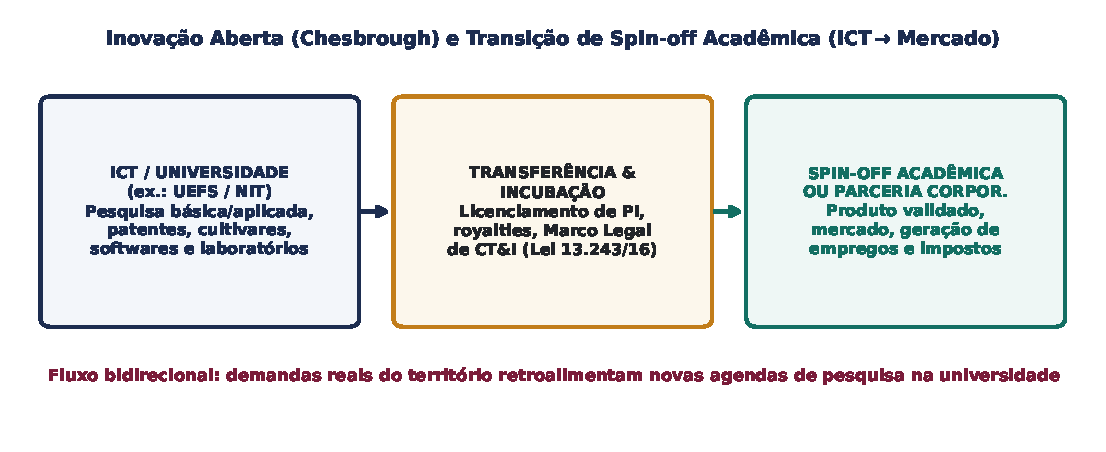
\includegraphics[width=0.94\textwidth]{figures/fig11_open_innovation_spinoff.pdf}
  \caption{Fluxos de \textit{Open Innovation} (\textit{inbound} e \textit{outbound}) e transição de \textit{spin-off} acadêmica da ICT/NIT para o mercado sob a Lei nº 13.243/2016.}
  \label{fig:11_open_innovation_spinoff}
\end{figure}

\begin{boxFormula}[Cálculo de \textit{Royalties} e Repartição Legal em Licenciamento de ICT (Lei 13.243/2016)]
  Considere uma \textit{spin-off} acadêmica (ou empresa licenciada) que comercializa um produto baseado em tecnologia protegida da ICT, obtendo faturamento líquido anual $F_{\text{líq}}$ (receita bruta deduzida de impostos sobre vendas e devoluções). Sendo $r$ a taxa contratual de \textit{royalty} (em decimal), a receita anual de licenciamento paga à ICT é:
  \[
    R_{\text{roy}} = F_{\text{líq}} \times r.
  \]
  De acordo com o art. 13 da Lei nº 10.973/2004 (atualizada pela Lei nº 13.243/2016), a parcela destinada aos criadores/inventores ($\alpha_{\text{inv}}$) deve situar-se no intervalo $0{,}05 \le \alpha_{\text{inv}} \le \frac{1}{3}$ (entre $5\%$ e $33{,}33\%$). Assim:
  \[
    G_{\text{inventores}} = R_{\text{roy}} \times \alpha_{\text{inv}}, \qquad
    G_{\text{ICT/NIT}} = R_{\text{roy}} \times (1 - \alpha_{\text{inv}}).
  \]
  Se houver $k$ inventores com participação igualitária na criação, cada inventor recebe $G_{\text{inventores}} / k$.
\end{boxFormula}

\etapa{4}{Estudos de Caso e Exemplos Resolvidos em 7 Passos}

\begin{boxExemplo}{11.1}{Licenciamento e Repartição de \textit{Royalties} em \textit{Spin-off} da UEFS}
  \passoEnunciado{Uma \textit{spin-off} fundada por egressos do PPGPT/UEFS licenciou junto ao NIT da universidade uma patente de sensor de umidade do solo de baixo custo.}
  \passoDados{Faturamento líquido anual da \textit{spin-off} com o sensor licenciado: $F_{\text{líq}} = \text{R\$\,1.200.000,00}$. Alíquota contratual de \textit{royalty}: $r = 4\%$ ($0{,}04$) sobre o faturamento líquido. Política de inovação da ICT: destina o teto legal de $\alpha_{\text{inv}} = 1/3$ ($33{,}33\%$) aos criadores (equipe de 2 inventores com partes iguais) e $2/3$ ($66{,}67\%$) à ICT/laboratório/NIT.}
  \passoPedido{Calcular o valor anual total de \textit{royalties} transferido à ICT, a parcela total dos inventores, o ganho individual de cada inventor e a parcela retida pela ICT/NIT.}
  \passoMetodo{Aplicação das equações de licenciamento e repartição conforme o art. 13 da Lei de Inovação.}
  \passoContas{
    Primeiro, calcula-se a receita total anual de \textit{royalties}:
    \[
      R_{\text{roy}} = 1.200.000,00 \times 0{,}04 = \text{R\$\,48.000,00/ano}.
    \]
    Em seguida, realiza-se a repartição entre os inventores ($1/3$) e a ICT/NIT ($2/3$):
    \[
      G_{\text{inventores}} = 48.000,00 \times \frac{1}{3} = \text{R\$\,16.000,00/ano},
    \]
    \[
      G_{\text{ICT/NIT}} = 48.000,00 \times \frac{2}{3} = \text{R\$\,32.000,00/ano}.
    \]
    Como há 2 inventores com participação igualitária, cada um recebe:
    \[
      G_{\text{por inventor}} = \frac{16.000,00}{2} = \text{R\$\,8.000,00/ano}.
    \]
  }
  \passoResposta{\textit{Royalties} totais $= \text{R\$\,48.000,00/ano}$; inventores $= \text{R\$\,16.000,00/ano}$ (R\$\,8.000,00 cada); ICT/NIT $= \text{R\$\,32.000,00/ano}$.}
  \passoVerificacao{Uma alíquota de 4\% sobre o faturamento líquido preserva a margem operacional da \textit{spin-off} enquanto gera retorno contínuo para retroalimentar o laboratório de origem.}
\end{boxExemplo}

\begin{boxExemplo}{11.2}{\textit{Open Innovation Inbound}: Licenciamento vs. P\&D Interno}
  \passoEnunciado{Uma indústria média de beneficiamento de couro e curtume no polo industrial de Feira de Santana precisa implantar um sistema de tratamento biológico de efluentes para atender à fiscalização ambiental.}
  \passoDados{Opção 1 (P\&D Interno fechado): investimento inicial de R\$\,600.000,00, prazo de desenvolvimento de 24 meses e custo de oportunidade por atraso de adequação ambiental de R\$\,15.000,00/mês. Opção 2 (\textit{Open Innovation Inbound}): licenciar tecnologia TRL 6 de uma ICT regional com taxa de adaptação de R\$\,180.000,00, prazo de 8 meses e pagamento fixo anual de licença de R\$\,36.000,00.}
  \passoPedido{Calcular a economia de CAPEX inicial, o ganho de tempo até a operação e o custo evitado de atraso na Opção 2.}
  \passoMetodo{Análise comparativa entre desenvolvimento fechado (\textit{make}) e incorporação aberta (\textit{buy/license}).}
  \passoContas{
    Economia de desembolso inicial (CAPEX de P\&D):
    \[
      \Delta \text{CAPEX} = 600.000,00 - 180.000,00 = \text{R\$\,420.000,00} \quad \left(\frac{420.000}{600.000} = 70{,}0\%\text{ de redução}\right).
    \]
    Ganho de tempo até a implantação: $24 - 8 = 16\text{ meses}$.
    Economia com custos evitados de atraso ambiental durante esses 16 meses:
    \[
      \text{Economia de atraso} = 16 \times 15.000,00 = \text{R\$\,240.000,00}.
    \]
    Mesmo pagando R\$\,36.000,00/ano de licença, os R\$\,420.000,00 economizados na entrada cobririam mais de 11 anos de anuidade de licenciamento.
  }
  \passoResposta{A estratégia \textit{inbound} reduz o CAPEX inicial em 70{,}0\% (R\$\,420.000,00), antecipa a operação em 16 meses e evita R\$\,240.000,00 em custos de atraso.}
  \passoVerificacao{O resultado explica por que médias empresas regionais sem laboratório próprio obtêm maior retorno adotando inovação aberta junto a ICTs.}
\end{boxExemplo}

\begin{boxExemplo}{11.3}{Empreendedorismo Corporativo e Renovação em Cooperativa Agroindustrial}
  \passoEnunciado{Uma cooperativa de processamento de mandioca observa queda de margem na venda de fécula comum e analisa uma proposta interna de dois engenheiros colaboradores para criar uma unidade de biogás e bioenergia a partir da manipueira (resíduo líquido tóxico do processamento).}
  \passoDados{Custo atual de descarte e tratamento da manipueira em lagoas: R\$\,14.000,00/mês. Investimento corporativo interno na planta de biodigestão: R\$\,480.000,00. Economia mensal de energia elétrica gerada pelo biogás: R\$\,16.000,00/mês (além de eliminar os R\$\,14.000,00/mês de custo de descarte).}
  \passoPedido{Classificar a iniciativa segundo Pinchot (1985) e Guth \& Ginsberg (1990) e calcular o ganho econômico mensal total e o \textit{payback} simples da unidade interna.}
  \passoMetodo{Identificação de intraempreendedorismo/renovação estratégica e cálculo de retorno sobre economia operacional.}
  \passoContas{
    Trata-se de \textbf{intraempreendedorismo} liderado pelos dois engenheiros e de \textbf{empreendedorismo corporativo} (criação de unidade interna de negócio e renovação ambiental da cooperativa).
    O benefício econômico mensal total soma a eliminação do custo de descarte e a economia de energia:
    \[
      \text{Benefício mensal} = 14.000,00 + 16.000,00 = \text{R\$\,30.000,00/mês}.
    \]
    O \textit{payback} simples do investimento corporativo de R\$\,480.000,00 é:
    \[
      \text{Payback} = \frac{480.000,00}{30.000,00} = 16\text{ meses}.
    \]
  }
  \passoResposta{A iniciativa gera benefício econômico de R\$\,30.000,00/mês e retorna o capital corporativo em 16 meses, convertendo um passivo ambiental em ativo energético.}
  \passoVerificacao{A infraestrutura já existente da cooperativa (fluxo garantido de manipueira e demanda própria de energia) elimina o risco comercial que uma startup independente enfrentaria.}
\end{boxExemplo}

\begin{boxExemplo}{11.4}{\textit{Open Innovation Outbound}: Monetização de Tecnologia Não Central}
  \passoEnunciado{Uma empresa de logística agrícola desenvolveu internamente um algoritmo de roteirização para estradas vicinais não pavimentadas do interior baiano. Como seu negócio principal é transporte de cargas próprias e não venda de software, o algoritmo atendia apenas à frota interna.}
  \passoDados{Custo adicional para empacotar a API para terceiros (\textit{outbound}): R\$\,45.000,00. Contrato de licenciamento não exclusivo para 15 cooperativas regionais a R\$\,1.500,00/mês por cooperativa.}
  \passoPedido{Calcular a receita anual bruta gerada pelo fluxo \textit{outbound} e em quantos meses o investimento de empacotamento é recuperado.}
  \passoMetodo{Análise de monetização de ativos ociosos via \textit{Open Innovation Outbound}.}
  \passoContas{
    Receita mensal do licenciamento para 15 cooperativas:
    \[
      R_{\text{mensal}} = 15 \times 1.500,00 = \text{R\$\,22.500,00/mês}.
    \]
    Receita anual bruta:
    \[
      R_{\text{anual}} = 22.500,00 \times 12 = \text{R\$\,270.000,00/ano}.
    \]
    Tempo para recuperar o custo de empacotamento da API (R\$\,45.000,00):
    \[
      \text{Payback} = \frac{45.000,00}{22.500,00} = 2{,}0\text{ meses}.
    \]
  }
  \passoResposta{O licenciamento \textit{outbound} gera R\$\,270.000,00/ano de nova receita com recuperação do custo de adaptação em apenas 2 meses.}
  \passoVerificacao{Em vez de deixar o ativo subutilizado dentro da firma ou tentar virar uma empresa de software concorrente do próprio negócio, a estratégia \textit{outbound} gera receita de alta margem.}
\end{boxExemplo}

\begin{boxExemplo}{11.5}{Intraempreendedorismo Público e Encomenda Tecnológica (ETEC)}
  \passoEnunciado{Um consórcio intermunicipal do Semiárido enfrenta recorrentes perdas de água em cisternas comunitárias por falta de detecção precoce de fissuras e contaminação microbiológica, sem encontrar solução comercial pronta no mercado para regiões sem cobertura celular.}
  \passoDados{Orçamento disponível para compras de emergência com caminhões-pipa: R\$\,900.000,00/ano. Uma servidora intraempreendedora propõe estruturar uma Encomenda Tecnológica (ETEC, art. 20 da Lei nº 10.973/2004) junto a uma ICT regional e uma startup local por R\$\,320.000,00 em 12 meses para desenvolver sensores autônomos via rádio LoRa.}
  \passoPedido{Explicar por que a licitação tradicional de menor preço falharia nesse caso e calcular a economia potencial se o sistema reduzir em 30\% o gasto anual com caminhões-pipa após implantado.}
  \passoMetodo{Aplicação do regime jurídico de ETEC (risco tecnológico) e estimativa de benefício fiscal territorial.}
  \passoContas{
    A licitação comum exige especificações técnicas já existentes no mercado; como há risco tecnológico inédito (sensores de baixo custo sem rede celular), a ETEC é o instrumento legal adequado.
    Se a solução reduzir em 30\% o gasto anual de R\$\,900.000,00 com caminhões-pipa, a economia anual será:
    \[
      \text{Economia anual} = 900.000,00 \times 0{,}30 = \text{R\$\,270.000,00/ano}.
    \]
    Comparando com o valor da ETEC (R\$\,320.000,00), o investimento público paga-se em $320.000 / 270.000 \approx 1{,}19\text{ ano}$ (cerca de 14{,}2 meses de operação).
  }
  \passoResposta{A ETEC viabiliza contratação pública sob risco tecnológico; a economia estimada de R\$\,270.000,00/ano recupera o investimento público em 1{,}19 ano.}
  \passoVerificacao{O intraempreendedorismo público transforma o poder de compra do Estado em motor de desenvolvimento tecnológico territorial.}
\end{boxExemplo}

\etapa{5}{Armadilhas Conceituais e Erros Mais Comuns}

\begin{boxErro}[Erro 1: Confundir \textit{Spin-off} Acadêmica com Projeto de Extensão sem Modelo de Negócio]
  Muitas equipes universitárias registram um CNPJ formal mantendo a lógica acadêmica de dependência exclusiva de bolsas, sem definir clientes pagantes, preços ou governança societária. Uma \textit{spin-off} exige separação clara entre a pesquisa acadêmica da ICT e a operação comercial autônoma da empresa.
\end{boxErro}

\begin{boxErro}[Erro 2: Fixar Taxas de \textit{Royalties} Proibitivas no Contrato com o NIT]
  Exigir \textit{royalties} elevados logo nos primeiros meses (ou pagamentos mínimos anuais desconectados da receita) inviabiliza a sobrevivência da \textit{spin-off} durante o Vale da Morte. A prática moderna adota taxas escalonadas ou vinculadas ao faturamento líquido após o início das vendas comerciais.
\end{boxErro}

\begin{boxErro}[Erro 3: Promover Intraempreendedorismo sem Autonomia nem Proteção contra Falhas]
  Pedir inovação aos colaboradores enquanto se pune qualquer experimento malsucedido com sanções na carreira destrói o intraempreendedorismo. Organizações precisam criar espaços protegidos de experimentação com métricas de aprendizado e perda aceitável definida.
\end{boxErro}

\begin{boxErro}[Erro 4: Tratar \textit{Open Innovation} como Terceirização Simples de Serviços]
  Contratar uma empresa de TI para executar um escopo fechado não é \textit{Open Innovation}. A inovação aberta envolve compartilhamento genuíno de risco, conhecimento tecnológico e propriedade intelectual entre parceiros externos e internos.
\end{boxErro}

\etapa{6}{Lista de Exercícios (15 Questões em 3 Níveis)}

\textbf{Nível 1, Fundamentos Conceituais (Questões 1 a 5)}

\begin{enumerate}[leftmargin=1.5em, itemsep=6pt]
  \item Diferencie intraempreendedorismo (Pinchot, 1985) de empreendedorismo corporativo (Guth \& Ginsberg, 1990) quanto ao nível de análise e aos resultados esperados na organização.
  \espacoResolucao[1.8cm]

  \item Explique a diferença entre \textit{Open Innovation Inbound} e \textit{Open Innovation Outbound}, citando um exemplo territorial para cada fluxo.
  \espacoResolucao[1.8cm]

  \item Qual é o papel do Núcleo de Inovação Tecnológica (NIT) na criação de uma \textit{spin-off} acadêmica sob a Lei nº 13.243/2016?
  \espacoResolucao[1.8cm]

  \item Cite três instrumentos previstos no Marco Legal de CT\&I (Lei nº 13.243/2016) que facilitam a transição da pesquisa universitária para o setor produtivo.
  \espacoResolucao[1.8cm]

  \item O que caracteriza o intraempreendedorismo público e em que situações a Encomenda Tecnológica (ETEC) substitui a licitação tradicional?
  \espacoResolucao[1.8cm]

  \item \textbf{(Nível 2, Aplicações Numéricas)} Uma \textit{spin-off} faturou R\$\,800.000,00 líquidos no ano com um produto licenciado de uma universidade pública, sob alíquota de \textit{royalty} de 5\%. Sabendo que a ICT destina 25\% dos ganhos aos inventores, calcule o total de \textit{royalties} pagos pela empresa, o valor recebido pelos inventores e o valor retido pela ICT/NIT.
  \espacoResolucao[2.3cm]

  \item No exercício anterior, se o pedido de patente teve 4 inventores com participação igualitária, quanto cada inventor recebeu no ano?
  \espacoResolucao[2.0cm]

  \item Uma cooperativa agroindustrial avalia duas opções para implantar rastreabilidade por QR Code: desenvolver internamente por R\$\,220.000,00 em 14 meses ou licenciar uma solução externa (\textit{inbound}) com implantação de R\$\,55.000,00 em 3 meses. Qual a economia percentual de desembolso inicial e quantos meses foram economizados?
  \espacoResolucao[2.2cm]

  \item Uma empresa licenciou em fluxo \textit{outbound} uma tecnologia não central para 8 empresas parceiras, cobrando taxa fixa de R\$\,2.500,00/mês por empresa. Sabendo que o custo anual de suporte técnico às licenciadas é de R\$\,40.000,00, qual é o ganho líquido anual gerado pelo licenciamento?
  \espacoResolucao[2.2cm]

  \item Um projeto de intraempreendedorismo em uma indústria têxtil exigiu R\$\,300.000,00 de investimento interno e passou a gerar economia mensal de água e insumos químicos de R\$\,25.000,00. Qual é o \textit{payback} simples desse projeto interno em meses?
  \espacoResolucao[2.1cm]

  \item \textbf{(Nível 3, Análise Territorial e Estratégica)} Analise por que uma \textit{spin-off} instalada em um município interiorano se beneficia mais do compartilhamento de laboratórios da ICT previsto na Lei nº 13.243/2016 do que da aquisição imediata de equipamentos próprios.
  \espacoResolucao[2.2cm]

  \item Uma universidade e uma \textit{spin-off} negociam contrato de licenciamento de patente. A \textit{spin-off} projeta faturamento líquido de R\$\,500.000,00 no Ano 1 e R\$\,1.500.000,00 no Ano 2. Compare dois modelos de cobrança pela ICT: Modelo A = taxa fixa anual de R\$\,60.000,00 desde o Ano 1; Modelo B = \textit{royalty} variável de 4\% sobre o faturamento líquido. Qual modelo protege melhor a \textit{spin-off} no Ano 1 e qual gera maior retorno acumulado para a ICT ao final dos 2 anos?
  \espacoResolucao[2.5cm]

  \item Discuta os principais conflitos de interesse que podem surgir quando um docente ou pesquisador público participa simultaneamente da ICT e de uma \textit{spin-off} acadêmica, e indique como a governança do NIT deve mitigá-los.
  \espacoResolucao[2.2cm]

  \item Uma prefeitura gasta R\$\,1.200.000,00/ano com coleta e destinação ineficiente de resíduos orgânicos de feiras livres. Um servidor intraempreendedor propõe uma ETEC de R\$\,240.000,00 com um instituto tecnológico para desenvolver biodigestor modular que reduza em 25\% o custo anual de destinação. Qual será a economia anual após a implantação e em quantos meses o investimento público se paga?
  \espacoResolucao[2.4cm]

  \item Elabore um fluxograma textual de 5 etapas mostrando como uma tecnologia protegida por uma ICT baiana percorre o caminho da bancada até o mercado via \textit{spin-off} acadêmica.
  \espacoResolucao[2.3cm]
\end{enumerate}

\etapa{7}{Questões Autorais Estilo Pós-Graduação / Concursos de CT\&I}

\begin{enumerate}[leftmargin=1.5em, itemsep=6pt]
  \item \textbf{(Estilo ANPAD / Gestão da Inovação)} Sobre inovação aberta (\textit{Open Innovation}) e empreendedorismo corporativo, assinale a alternativa correta:
  \begin{alternativas}
    \item O fluxo \textit{outbound} ocorre quando uma empresa adquire startups externas para substituir seu departamento de vendas.
    \item O empreendedorismo corporativo, segundo Guth e Ginsberg (1990), limita-se à criação de programas de sugestões de baixo custo sem impacto na estratégia da empresa.
    \item O fluxo \textit{inbound} permite à empresa absorver tecnologias externas desenvolvidas por ICTs ou startups, reduzindo tempo de desenvolvimento e risco técnico.
    \item Na inovação fechada, as empresas priorizam o licenciamento de patentes ociosas para concorrentes regionais.
    \item O intraempreendedorismo exige obrigatoriamente que o colaborador peça demissão para fundar uma empresa independente.
  \end{alternativas}
  \espacoResolucao[1.5cm]

  \item \textbf{(Estilo Concurso Gestor de CT\&I / NIT)} Uma ICT licenciou patente de bioinsumo para uma \textit{spin-off} sob taxa de \textit{royalty} de 3\% sobre o faturamento líquido. No exercício anual, a \textit{spin-off} faturou R\$\,2.000.000,00 líquidos. Sabendo que a política de inovação da ICT fixa a participação dos inventores no limite máximo permitido pela Lei nº 10.973/2004 (1/3 dos ganhos econômicos), o valor destinado aos inventores e o valor retido pela ICT são, respectivamente:
  \begin{alternativas}
    \item R\$\,3.000,00 e R\$\,57.000,00.
    \item R\$\,20.000,00 e R\$\,40.000,00.
    \item R\$\,15.000,00 e R\$\,45.000,00.
    \item R\$\,30.000,00 e R\$\,30.000,00.
    \item R\$\,60.000,00 e R\$\,120.000,00.
  \end{alternativas}
  \espacoResolucao[1.6cm]

  \item \textbf{(Estilo Discursiva, PPGPT)} Explique como o intraempreendedorismo público e a Encomenda Tecnológica (ETEC) previstos no Marco Legal de CT\&I podem atuar como indutores de sistemas locais de inovação em municípios de pequeno e médio porte.
  \espacoResolucao[2.3cm]
\end{enumerate}

\begin{boxDica}[Contraponto Crítico e Prática Territorial (AV3)]
  Se o seu Projeto Final (AV3) nasce de uma pesquisa de laboratório (ICT/UEFS) ou ocorre dentro de uma cooperativa/órgão público, explicite na seção estratégica qual é o regime de transferência tecnológica (licenciamento via NIT, compartilhamento de laboratório, *spin-off* ou intraempreendedorismo) e apresente o cálculo de *royalties* ou economia operacional esperado.
\end{boxDica}

\clearpage
\etapa{8}{Gabarito Integralmente Comentado (Exercícios 1 a 18)}

\begin{boxGabarito}[Resolução Completa dos Exercícios da Etapa 6 (1 a 15) e Etapa 7 (16 a 18)]
  \begin{enumerate}[leftmargin=1.5em, itemsep=4pt]
    \item \textbf{Resposta:} Intraempreendedorismo (Pinchot) foca a ação empreendedora de colaboradores dentro da organização; empreendedorismo corporativo (Guth \& Ginsberg) foca o nível estratégico da firma via criação de novos negócios (\textit{corporate venturing}) e renovação estratégica.
    \item \textbf{Resposta:} \textit{Inbound} é trazer tecnologia externa para dentro (ex.: indústria local licenciando biofilme de universidade); \textit{Outbound} é levar tecnologia interna para fora (ex.: empresa de logística licenciando algoritmo ocioso para cooperativas).
    \item \textbf{Resposta:} O NIT protege a PI da ICT, realiza busca de anterioridade, negocia contratos de transferência de tecnologia e licenciamento, e orienta a formalização da relação entre ICT e \textit{spin-off}.
    \item \textbf{Resposta:} Compartilhamento de laboratórios/infraestrutura da ICT com empresas; participação dos criadores em 5\% a 1/3 dos ganhos econômicos; Encomenda Tecnológica (ETEC) pelo poder público.
    \item \textbf{Resposta:} Intraempreendedorismo público é a inovação liderada por servidores dentro da administração pública. A ETEC substitui a licitação tradicional quando a solução desejada ainda não existe no mercado e envolve risco tecnológico inédito.
    \item \textbf{Resposta:} $R_{\text{roy}} = 800.000 \times 0{,}05 = \text{R\$\,40.000,00/ano}$. Parcela dos inventores $= 40.000 \times 0{,}25 = \text{R\$\,10.000,00/ano}$. Parcela da ICT/NIT $= 40.000 - 10.000 = \text{R\$\,30.000,00/ano}$.
    \item \textbf{Resposta:} Cada inventor recebeu $10.000,00 / 4 = \text{R\$\,2.500,00/ano}$.
    \item \textbf{Resposta:} Economia $= 220.000 - 55.000 = \text{R\$\,165.000,00}$, o que equivale a $165.000 / 220.000 = 75{,}0\%$ de redução no desembolso inicial. Economia de tempo $= 14 - 3 = 11\text{ meses}$.
    \item \textbf{Resposta:} Receita bruta anual $= 8 \times 2.500 \times 12 = \text{R\$\,240.000,00/ano}$. Ganho líquido anual $= 240.000 - 40.000 = \text{R\$\,200.000,00/ano}$.
    \item \textbf{Resposta:} $\text{Payback} = 300.000 / 25.000 = 12\text{ meses}$.
    \item \textbf{Resposta:} Porque reduz drasticamente o CAPEX inicial na fase TRL 3–6, evitando que a \textit{spin-off} imobilize capital escasso em equipamentos analíticos caros antes de validar vendas recorrentes no território.
    \item \textbf{Resposta:} Modelo A (fixo): Ano 1 = R\$\,60.000; Ano 2 = R\$\,60.000; Total 2 anos = R\$\,120.000. Modelo B (4\%): Ano 1 = $500.000 \times 0{,}04 = \text{R\$\,20.000}$; Ano 2 = $1.500.000 \times 0{,}04 = \text{R\$\,60.000}$; Total 2 anos = R\$\,80.000. O Modelo B protege melhor a \textit{spin-off} no Ano 1 (reduz o peso de R\$\,60 mil para R\$\,20 mil na fase inicial), enquanto o Modelo A gera maior retorno acumulado à ICT (R\$\,120 mil vs. R\$\,80 mil).
    \item \textbf{Resposta:} Conflitos comuns envolvem uso indevido de horas de dedicação exclusiva, desvio de insumos públicos ou favorecimento sem registro. Mitigam-se com declarações formais de conflito de interesse, contratos de compartilhamento precificados via NIT e separação contábil e societária.
    \item \textbf{Resposta:} Economia anual $= 1.200.000 \times 0{,}25 = \text{R\$\,300.000,00/ano}$ (equivalente a R\$\,25.000,00/mês). Tempo de retorno da ETEC $= 240.000 / 25.000 = 9{,}6\text{ meses}$ (ou $0{,}8\text{ ano}$).
    \item \textbf{Resposta:} (1) Invenção e comunicação de invento ao NIT; (2) Busca de anterioridade e depósito de PI; (3) Constituição da \textit{spin-off} e negociação de contrato de licenciamento/compartilhamento; (4) Captação de fomento (Centelha/FAPESB/FINEP) para travessia TRL 4–7; (5) Comercialização e pagamento de \textit{royalties} à ICT/inventores.
    \item \textbf{Questão 16 (Etapa 7), Gabarito: (C).} O fluxo \textit{inbound} consiste exatamente na incorporação de conhecimento e tecnologia externa.
    \item \textbf{Questão 17 (Etapa 7), Gabarito: (B).} $R_{\text{roy}} = 2.000.000 \times 0{,}03 = \text{R\$\,60.000,00}$. Inventores $= 60.000 / 3 = \text{R\$\,20.000,00}$. ICT $= 60.000 - 20.000 = \text{R\$\,40.000,00}$.
    \item \textbf{Questão 18 (Etapa 7), Espelho Discursivo:} Deve explicar que o poder de compra municipal/consortiado direcionado via ETEC cria demanda garantida para problemas locais específicos, estimulando ICTs e startups regionais a desenvolverem soluções tecnológicas territorializadas sem depender de importação.
  \end{enumerate}
\end{boxGabarito}

\begin{boxResumo}
  \begin{itemize}[leftmargin=1.4em, itemsep=2pt]
    \item Intraempreendedorismo e empreendedorismo corporativo renovam organizações existentes aproveitando ativos complementares já instalados.
    \item A inovação aberta integra fluxos \textit{inbound} (redução de custo e tempo de P\&D) e \textit{outbound} (monetização de tecnologias fora do negócio central).
    \item A Lei nº 13.243/2016 viabiliza \textit{spin-offs} acadêmicas, compartilhamento de laboratórios, repartição legal de \textit{royalties} (5\% a 1/3 aos inventores) e Encomendas Tecnológicas (ETEC) no setor público.
  \end{itemize}
\end{boxResumo}

\begin{boxTeste}
  \begin{enumerate}[leftmargin=1.5em, itemsep=4pt]
    \item (\V/\F) Na inovação aberta, o fluxo \textit{outbound} refere-se à compra de tecnologia externa para uso exclusivo dentro da fábrica.
    \item (\V/\F) Pela Lei nº 10.973/2004 (alterada pela Lei nº 13.243/2016), os inventores têm direito a uma parcela entre 5\% e 1/3 dos ganhos econômicos auferidos pela ICT com o licenciamento.
    \item (\V/\F) Se uma ICT recebe R\$\,90.000,00 de \textit{royalties} no ano e destina 20\% aos inventores, a ICT retém R\$\,72.000,00 e os inventores recebem R\$\,18.000,00.
    \item (\V/\F) A Encomenda Tecnológica (ETEC) permite ao poder público contratar o desenvolvimento de solução inédita com risco tecnológico junto a ICTs ou empresas.
  \end{enumerate}
  \begin{boxGabarito}[Respostas do Checkpoint: Capítulo 11]
    \textbf{1: \F} (Isso é \textit{inbound}; \textit{outbound} é externalizar tecnologia própria). \quad \textbf{2: \V}. \quad \textbf{3: \V} ($90.000 \times 0{,}20 = 18.000$; $90.000 - 18.000 = 72.000$). \quad \textbf{4: \V}.
  \end{boxGabarito}
\end{boxTeste}

\clearpage
\phantomsection
\addcontentsline{toc}{chapter}{Simulado II: Revisão Integrada da Unidade II}
\chapter*{Simulado II: Revisão Integrada da Unidade II (Processo e Estratégia)}
\markboth{SIMULADO II, UNIDADE II}{SIMULADO II, UNIDADE II}

\noindent\tagAV{Base AV3} \tagQuant\ \tagTerritorio

\begin{tcolorbox}[colback=bgSoft, colframe=etIndigo, arc=3pt, boxrule=0.7pt, left=10pt, right=10pt, top=7pt, bottom=7pt]
  \textbf{Instruções para Estudo Autônomo:} Este simulado integra os conteúdos dos \textbf{Capítulos 7 a 11} (Unidade II, Processo e Estratégia). Resolva as \textbf{8 questões objetivas (A–E)} e as \textbf{2 questões dissertativas} sem consultar o gabarito. Ao concluir, confira o gabarito comentado, o espelho dissertativo e preencha a Tabela de Diagnóstico na página seguinte.
\end{tcolorbox}

\section*{Parte A: Questões Objetivas (Capítulos 7 a 11)}

\begin{enumerate}[leftmargin=1.5em, itemsep=8pt]
  \item \textbf{(Cap. 7, Processo Empreendedor e \textit{Effectuation})} Um grupo de pesquisadores da UEFS desenvolveu um sensor óptico para detectar adulteração em méis regionais. Sem histórico de vendas desse dispositivo, decidiram limitar o investimento inicial a R\$\,15.000,00 próprios e firmar pré-compromisso com duas cooperativas de apicultores que cederam amostras e espaço de teste em troca de prioridade no uso. À luz de Sarasvathy (2001), essa estratégia exemplifica, respectivamente, os princípios:
  \begin{alternativas}
    \item Causation preditiva e maximização do retorno esperado.
    \item Perda aceitável (\textit{affordable loss}) e colcha de retalhos (\textit{crazy quilt}).
    \item Limonada (\textit{lemonade}) e análise competitiva de Porter.
    \item Piloto no avião e planejamento causal de longo prazo.
    \item Nexo indivíduo–oportunidade e diluição acionária.
  \end{alternativas}
  \espacoResolucao[1.2cm]

  \item \textbf{(Cap. 7, Curva J e Vale da Morte Tecnológico)} Uma startup de biotecnologia apresenta os seguintes fluxos de caixa líquidos anuais (em R\$): Ano 0 = $-90.000$; Ano 1 = $-110.000$; Ano 2 = $-40.000$; Ano 3 = $+120.000$; Ano 4 = $+160.000$. O fundo do Vale da Morte e o prazo de \textit{payback} simples desse empreendimento são, respectivamente:
  \begin{alternativas}
    \item $-\text{R\$\,200.000,00}$ no Ano 1 e 3{,}50 anos.
    \item $-\text{R\$\,240.000,00}$ no Ano 2 e 3{,}75 anos.
    \item $-\text{R\$\,240.000,00}$ no Ano 2 e 3{,}25 anos.
    \item $-\text{R\$\,120.000,00}$ no Ano 3 e 4{,}00 anos.
    \item $-\text{R\$\,240.000,00}$ no Ano 1 e 2{,}75 anos.
  \end{alternativas}
  \espacoResolucao[1.5cm]

  \item \textbf{(Cap. 8, Dimensionamento TAM, SAM e SOM)} Uma empresa desenvolveu uma plataforma de gestão hídrica para pequenas agroindústrias. No Brasil existem $50.000$ agroindústrias desse porte, com gasto médio potencial de R\$\,2.400,00/ano. O recorte regional do Nordeste e perfil aderente representa 30\% desse universo. Sabendo que a equipe comercial tem capacidade operacional (\textit{bottom-up}) para atender no máximo $450$ agroindústrias por ano no horizonte de 3 anos, o TAM, o SAM e o SOM \textit{bottom-up} anuais são, respectivamente:
  \begin{alternativas}
    \item R\$\,120,0 milhões; R\$\,36,0 milhões; R\$\,1,08 milhão.
    \item R\$\,120,0 milhões; R\$\,18,0 milhões; R\$\,1,08 milhão.
    \item R\$\,36,0 milhões; R\$\,10,8 milhões; R\$\,1,08 milhão.
    \item R\$\,120,0 milhões; R\$\,36,0 milhões; R\$\,3,60 milhões.
    \item R\$\,60,0 milhões; R\$\,36,0 milhões; R\$\,0,90 milhão.
  \end{alternativas}
  \espacoResolucao[1.5cm]

  \item \textbf{(Cap. 8, Propriedade Intelectual e Anterioridade)} Uma startup baiana desenvolveu um método inédito de extração enzimática de óleo de licuri (processo industrial) e um algoritmo de controle de temperatura embarcado no extrator. Uma busca no INPI identificou que o processo enzimático não possui anterioridade mundial, mas o algoritmo de controle baseia-se em código aberto sob licença permissiva. A estratégia de proteção mais adequada para os ativos próprios da startup é:
  \begin{alternativas}
    \item Modelo de Utilidade para o algoritmo e Marca Coletiva para o processo enzimático.
    \item Patente de Invenção para o processo enzimático inédito e Segredo Industrial ou Registro de Software apenas para as adaptações proprietárias do controle, respeitando a licença do código-base.
    \item Indicação Geográfica para o processo enzimático e Cultivar para o extrator mecânico.
    \item Patente de Invenção para o código aberto de terceiros e Direito Autoral para o óleo de licuri.
    \item Nenhuma proteção é possível, pois o uso de qualquer componente de código aberto impede o depósito de patente do processo químico.
  \end{alternativas}
  \espacoResolucao[1.2cm]

  \item \textbf{(Cap. 9, \textit{Business Model Canvas} e Economia Unitária)} Um serviço de monitoramento de solo por assinatura cobra $\text{ARPU} = \text{R\$\,400,00/mês}$, opera com margem bruta de 75\% e apresenta taxa mensal de \textit{churn} de 5\%. Se a empresa gastou R\$\,15.000,00 em marketing e vendas para adquirir 10 novos clientes no mês, o CAC, o LTV e a razão LTV/CAC são, respectivamente:
  \begin{alternativas}
    \item $\text{CAC} = \text{R\$\,1.500,00}$; $\text{LTV} = \text{R\$\,8.000,00}$; $\text{LTV/CAC} = 5{,}33$.
    \item $\text{CAC} = \text{R\$\,1.500,00}$; $\text{LTV} = \text{R\$\,6.000,00}$; $\text{LTV/CAC} = 4{,}00$.
    \item $\text{CAC} = \text{R\$\,1.000,00}$; $\text{LTV} = \text{R\$\,6.000,00}$; $\text{LTV/CAC} = 6{,}00$.
    \item $\text{CAC} = \text{R\$\,1.500,00}$; $\text{LTV} = \text{R\$\,4.500,00}$; $\text{LTV/CAC} = 3{,}00$.
    \item $\text{CAC} = \text{R\$\,3.000,00}$; $\text{LTV} = \text{R\$\,6.000,00}$; $\text{LTV/CAC} = 2{,}00$.
  \end{alternativas}
  \espacoResolucao[1.5cm]

  \item \textbf{(Cap. 10, Escada do Capital e Indicadores de Tração)} Uma empresa de base tecnológica possui caixa disponível de R\$\,320.000,00, despesas operacionais mensais totais (\textit{Gross Burn}) de R\$\,60.000,00 e 50 clientes pagando assinatura mensal de R\$\,400,00. Considerando essas condições constantes, o MRR, o \textit{Net Burn} e o \textit{Runway} estático são, respectivamente:
  \begin{alternativas}
    \item $\text{MRR} = \text{R\$\,20.000,00}$; $\text{Net Burn} = \text{R\$\,40.000,00/mês}$; $\text{Runway} = 8{,}0\text{ meses}$.
    \item $\text{MRR} = \text{R\$\,20.000,00}$; $\text{Net Burn} = \text{R\$\,60.000,00/mês}$; $\text{Runway} = 5{,}3\text{ meses}$.
    \item $\text{MRR} = \text{R\$\,25.000,00}$; $\text{Net Burn} = \text{R\$\,35.000,00/mês}$; $\text{Runway} = 9{,}1\text{ meses}$.
    \item $\text{MRR} = \text{R\$\,20.000,00}$; $\text{Net Burn} = \text{R\$\,40.000,00/mês}$; $\text{Runway} = 16{,}0\text{ meses}$.
    \item $\text{MRR} = \text{R\$\,30.000,00}$; $\text{Net Burn} = \text{R\$\,30.000,00/mês}$; $\text{Runway} = 10{,}7\text{ meses}$.
  \end{alternativas}
  \espacoResolucao[1.5cm]

  \item \textbf{(Cap. 10, Fomento Regional e Diluição)} Assinale a alternativa que apresenta o alinhamento correto entre estágio tecnológico e instrumento da Escada do Capital para uma EBT localizada na Bahia:
  \begin{alternativas}
    \item TRL 2–3 deve ser financiado prioritariamente por crédito bancário comercial de curto prazo com garantia real dos sócios.
    \item Subvenções econômicas como Programa Centelha, FAPESB e FINEP Tecnova têm caráter não dilutivo e compartilham o risco tecnológico na travessia TRL 3–6.
    \item O FNE Inovação do Banco do Nordeste atua exclusivamente como capital de risco (\textit{equity}), exigindo assento no conselho e cessão de 20\% das quotas.
    \item Investidores-anjo substituem a necessidade de validação de MVP, pois aportam capital apenas em ideias sem contato prévio com clientes.
    \item O \textit{Pitch Deck} substitui integralmente o Plano de Negócio Completo na aprovação de linhas de financiamento industrial do BNDES.
  \end{alternativas}
  \espacoResolucao[1.2cm]

  \item \textbf{(Cap. 11, \textit{Open Innovation}, \textit{Spin-offs} e Lei nº 13.243/2016)} Uma \textit{spin-off} acadêmica licenciou junto ao NIT de uma universidade pública uma patente de biofilme para frutas sob alíquota de \textit{royalty} de 5\% sobre o faturamento líquido. No ano de referência, a empresa obteve faturamento líquido de R\$\,1.000.000,00 com o produto. Sabendo que a resolução interna da ICT destina 30\% dos ganhos econômicos aos inventores (dentro do intervalo legal de 5\% a 1/3 da Lei nº 10.973/2004), o valor anual transferido aos inventores e o valor retido pela ICT/NIT são, respectivamente:
  \begin{alternativas}
    \item R\$\,50.000,00 e R\$\,100.000,00.
    \item R\$\,15.000,00 e R\$\,35.000,00.
    \item R\$\,16.666,67 e R\$\,33.333,33.
    \item R\$\,25.000,00 e R\$\,25.000,00.
    \item R\$\,5.000,00 e R\$\,45.000,00.
  \end{alternativas}
  \espacoResolucao[1.5cm]
\end{enumerate}

\section*{Parte B: Questões Dissertativas (Integração Estratégica e Territorial)}

\begin{enumerate}[leftmargin=1.5em, itemsep=8pt, start=9]
  \item \textbf{(Integração Caps. 7, 8 e 9, Do Vale da Morte ao Modelo de Negócio)} Um laboratório universitário desenvolveu um secador solar automatizado para amêndoas de cacau (TRL 4), mas não encontra compradores dispostos a pagar R\$\,35.000,00 à vista pelo equipamento. Proponha uma estratégia integrada de travessia do Vale da Morte combinando: (a) dois princípios de \textit{Effectuation}; (b) cruzamento de SOM \textit{bottom-up}; e (c) reformulação do bloco Fontes de Receita do \textit{Business Model Canvas} (Chesbrough \& Rosenbloom, 2002).
  \espacoResolucao[2.8cm]

  \item \textbf{(Integração Caps. 10 e 11, Escada do Capital e \textit{Spin-off} Acadêmica)} Explique como uma \textit{spin-off} acadêmica originada em uma ICT pública pode combinar a Lei nº 13.243/2016 (compartilhamento de laboratórios e licenciamento via NIT) com os degraus da Escada do Capital (Centelha/FAPESB/FINEP $\to$ anjo $\to$ FNE Inovação) para reduzir a diluição societária dos fundadores antes de captar \textit{Venture Capital}.
  \espacoResolucao[2.8cm]
\end{enumerate}

\clearpage
\section*{Gabarito Comentado, Espelho Dissertativo e Diagnóstico: Simulado II}

\begin{boxGabarito}[Gabarito Comentado das Questões Objetivas (1 a 8)]
  \begin{enumerate}[leftmargin=1.5em, itemsep=4pt]
    \item \textbf{Gabarito: (B).} Limitar o desembolso a R\$\,15.000,00 próprios corresponde à perda aceitável (\textit{affordable loss}); firmar pré-compromissos com cooperativas para co-testar o produto corresponde à colcha de retalhos (\textit{crazy quilt}).
    \item \textbf{Gabarito: (B).} $FCA_0 = -90.000$; $FCA_1 = -200.000$; $FCA_2 = -240.000$ (fundo do Vale da Morte); $FCA_3 = -120.000$; $FCA_4 = +40.000$. $\text{Payback} = 3 + 120.000 / 160.000 = 3{,}75\text{ anos}$.
    \item \textbf{Gabarito: (A).} $\text{TAM} = 50.000 \times 2.400 = \text{R\$\,120.000.000,00}$ (R\$\,120,0 milhões). $\text{SAM} = 120.000.000 \times 0{,}30 = \text{R\$\,36.000.000,00}$ (R\$\,36,0 milhões). $\text{SOM}_{\text{BU}} = 450 \times 2.400 = \text{R\$\,1.080.000,00}$ (R\$\,1,08 milhão).
    \item \textbf{Gabarito: (B).} Processos industriais inéditos são protegidos por Patente de Invenção; o código proprietário agregado pode ser protegido por Registro de Software ou Segredo Industrial, observando os termos da licença aberta utilizada na base.
    \item \textbf{Gabarito: (B).} $\text{CAC} = 15.000 / 10 = \text{R\$\,1.500,00}$. $\text{MC}_{\text{mensal}} = 400 \times 0{,}75 = \text{R\$\,300,00}$. Retenção $= 1 / 0{,}05 = 20\text{ meses}$. $\text{LTV} = 300 \times 20 = \text{R\$\,6.000,00}$. $\text{LTV/CAC} = 6.000 / 1.500 = 4{,}00$.
    \item \textbf{Gabarito: (A).} $\text{MRR} = 50 \times 400 = \text{R\$\,20.000,00}$. $\text{Net Burn} = 60.000 - 20.000 = \text{R\$\,40.000,00/mês}$. $\text{Runway} = 320.000 / 40.000 = 8{,}0\text{ meses}$.
    \item \textbf{Gabarito: (B).} Subvenções não exigem participação societária nem devolução do principal, atuando exatamente na travessia TRL 3–6; crédito FNE é reembolsável (não é \textit{equity}).
    \item \textbf{Gabarito: (B).} $R_{\text{roy}} = 1.000.000 \times 0{,}05 = \text{R\$\,50.000,00}$. Parcela dos inventores $= 50.000 \times 0{,}30 = \text{R\$\,15.000,00}$. Parcela da ICT/NIT $= 50.000 - 15.000 = \text{R\$\,35.000,00}$.
  \end{enumerate}
\end{boxGabarito}

\begin{boxGabarito}[Espelho Dissertativo: Questões 9 e 10]
  \begin{itemize}[leftmargin=1.4em, itemsep=4pt]
    \item \textbf{Questão 9 (Critérios de Correção):}
    (a) \textit{Effectuation}: mobilizar \textit{Pássaro na mão} (uso do laboratório universitário para protótipos) e \textit{Colcha de retalhos} (cooperativa cacaueira cede amêndoas e galpão para validar TRL 5–6 com perda aceitável definida).
    (b) \textit{SOM bottom-up}: estimar quantas unidades a oficina local consegue montar e instalar por ano multiplicado pelo preço/assinatura anual, confrontando com o SAM do Sul da Bahia.
    (c) \textit{Fontes de Receita / BMC}: substituir venda de ativo por assinatura/serviço (HaaS ou cobrança por lote secado), eliminando a barreira de R\$\,35.000,00 de CAPEX inicial do produtor.
    \item \textbf{Questão 10 (Critérios de Correção):}
    Deve articular que o compartilhamento de infraestrutura da ICT (Lei nº 13.243/2016) e o licenciamento com *royalties* variáveis via NIT reduzem o \textit{Burn Rate} inicial. Ao combinar isso com subvenções não dilutivas (Centelha, FAPESB, FINEP) para elevar a maturidade de TRL 3 a TRL 6–7 e gerar MRR inicial, a \textit{spin-off} aumenta seu \textit{valuation pre-money} antes de buscar investidor-anjo ou \textit{Venture Capital} (e pode usar crédito FNE Inovação para planta produtiva), preservando maior participação dos fundadores.
  \end{itemize}
\end{boxGabarito}

\section*{Tabela de Diagnóstico e Plano de Revisão (Unidade II)}

\begin{center}
\renewcommand{\arraystretch}{1.24}
\small
\begin{tabularx}{\textwidth}{@{}c l >{\raggedright\arraybackslash}X l@{}}
  \toprule
  \rowcolor{etIndigo}
  \textcolor{white}{\bfseries Questões} & \textcolor{white}{\bfseries Capítulo} & \textcolor{white}{\bfseries Competência Avaliada} & \textcolor{white}{\bfseries Acerto (\checkmark / $\times$)} \\
  \midrule
  1 e 2 & Cap. 7 & \textit{Effectuation}, Curva J, Vale da Morte e \textit{payback} & \rule{1.8cm}{0.4pt} \\
  \rowcolor{bgGray}
  3 e 4 & Cap. 8 & TAM/SAM/SOM (\textit{top-down}/\textit{bottom-up}) e PI/FTO & \rule{1.8cm}{0.4pt} \\
  5 & Cap. 9 & BMC, \textit{Lean Startup}, CAC, LTV e razão LTV/CAC & \rule{1.8cm}{0.4pt} \\
  \rowcolor{bgGray}
  6 e 7 & Cap. 10 & Escada do Capital, fomento regional, MRR, \textit{Burn} e \textit{Runway} & \rule{1.8cm}{0.4pt} \\
  8 & Cap. 11 & \textit{Open Innovation}, \textit{spin-off}, NIT e \textit{royalties} (Lei 13.243/2016) & \rule{1.8cm}{0.4pt} \\
  \rowcolor{bgTeal}
  9 e 10 & Síntese & Integração estratégica e territorial para a AV3 & \rule{1.8cm}{0.4pt} \\
  \bottomrule
\end{tabularx}
\end{center}


% --- UNIDADE III — PROJETOS E VIABILIDADE ---
\aberturaModulo{UNIDADE III}{PROJETOS E VIABILIDADE}{Encontros 12 a 14 $\bullet$ Base da AV2 (20\%) e Engenharia Financeira da AV3}{%
Esta unidade converte a estratégia territorial e o modelo de negócios da Unidade II em engenharia econômica e modelagem financeira auditável. Ao longo de três encontros e um simulado quantitativo, o estudante aprende a estruturar projetos executivos de investimento, decidir sua localização territorial com rigor multicritério, projetar fluxos de caixa livres, aplicar métricas de viabilidade sob risco e estimar o valor econômico de empreendimentos tecnológicos e de impacto.
\begin{itemize}[leftmargin=1.4em, itemsep=3pt]
  \item \textbf{Capítulo 12: Elaboração de Projetos de Investimento e Decisão Locacional:} ciclo do projeto (Woiler \& Mathias, 2008), fatores locacionais clássicos (Weber, Von Thünen), Matriz Locacional Ponderada, orçamento de CAPEX, Ciclo Financeiro / Capital de Giro (NLCG), OPEX e Ponto de Equilíbrio Contábil.
  \item \textbf{Capítulo 13: Métodos e Ferramentas para Análise de Investimentos:} valor do dinheiro no tempo, Fluxo de Caixa Livre (FCL), VPL, TIR (e suas anomalias), MTIR, VAUE para vidas úteis distintas, Payback Simples e Descontado, análise de sensibilidade e cenários.
  \item \textbf{Capítulo 14: Valuation de Empreendimentos Tecnológicos e Projetos de Impacto:} preço versus valor, Fluxo de Caixa Descontado (Damodaran, 2010), WACC, perpetuidade de Gordon, Enterprise Value e Equity Value, \textit{Dark Side of Valuation}, Método de Venture Capital e Opções Reais.
  \item \textbf{Simulado III: Preparatório Quantitativo da AV2 (20\%):} 8 questões objetivas de cálculo integral (A--E), 2 estudos dirigidos dissertativos, gabarito passo a passo, espelho e diagnóstico.
\end{itemize}
}

\chapter{Elaboração de Projetos de Investimento e Decisão Locacional}
\label{cap:12}

\noindent\tagAV{AV2 (20\%)}\ \tagQuant\ \tagTerritorio
\vspace{6pt}

\begin{capObjetivos}
Ao concluir este capítulo, você será capaz de:
\begin{enumerate}[leftmargin=1.4em, itemsep=2pt]
  \item Estruturar a passagem da ideia empreendedora ao projeto executivo de investimento segundo o ciclo de estudo de mercado, engenharia, localização e orçamento (Woiler \& Mathias, 2008).
  \item Avaliar alternativas territoriais combinando fatores locacionais clássicos (Weber e Von Thünen), infraestrutura energética e hídrica, densidade de P\&D e incentivos fiscais por meio da \textbf{Matriz Locacional Ponderada}.
  \item Dimensionar a estrutura orçamentária completa de um projeto: investimento fixo (\textbf{CAPEX}), Necessidade Líquida de Capital de Giro (\textbf{NLCG}) derivada do ciclo financeiro e custos operacionais (\textbf{OPEX}).
  \item Calcular e interpretar o \textbf{Ponto de Equilíbrio Contábil} (em unidades e em receita) e a margem de segurança operacional diante de variações locacionais e tributárias.
\end{enumerate}
\end{capObjetivos}

\begin{capRevisao}
Antes de avançar para a modelagem orçamentária e locacional, relembre três fundamentos das Unidades I e II:
\begin{itemize}[leftmargin=1.4em, itemsep=2pt]
  \item \textbf{Aglomerações e Eficiência Coletiva (Cap. 2):} a localização não é apenas custo de frete; proximidade a fornecedores especializados, universidades e mão de obra qualificada gera economias externas que reduzem custos unitários e aceleram o aprendizado tecnológico.
  \item \textbf{Proposta de Valor e Estrutura de Custos no Canvas (Cap. 9):} todo bloco de atividades-chave e recursos-chave do modelo de negócios precisa ser traduzido em imobilizações (CAPEX) e despesas recorrentes (OPEX) para que o empreendimento saia do plano discursivo.
  \item \textbf{Instrumentos de Fomento Regional (Cap. 10):} linhas como BNB/FNE, BNDES, FINEP e FAPESB financiam parcelas distintas do projeto (máquinas, obras, P\&D ou capital de giro), exigindo separação contábil clara entre investimento fixo e giro.
\end{itemize}
\end{capRevisao}

\etapa{3}{Fundamentação Teórica, Fatores Locacionais e Orçamento do Projeto}

\subsection{Da ideia ao projeto executivo (Woiler \& Mathias, 2008)}

Uma ideia tecnológica ou territorialmente enraizada só se torna financiável quando convertida em um \textbf{projeto de investimento}, isto é, um conjunto sistematizado de informações técnicas, mercadológicas, locacionais, jurídicas e econômico-financeiras que permite decidir se vale a pena imobilizar recursos escassos hoje em troca de benefícios futuros incertos. Na tradição brasileira de elaboração e análise de projetos sistematizada por Woiler e Mathias (2008), essa trajetória percorre três estágios progressivos de redução de incerteza, nos quais cada etapa filtra riscos antes de comprometer capital em engenharia dispendiosa.

No estágio inicial de \textbf{Identificação da Oportunidade e Estudo de Pré-Viabilidade}, você delimita o problema territorial ou tecnológico, estima a demanda potencial (TAM/SAM/SOM) e verifica restrições legais ou ambientais eliminatórias antes de gastar com engenharia detalhada. Superada essa triagem preliminar, o \textbf{Anteprojeto ou Estudo de Viabilidade Técnica e Econômica (EVTE)} define a escala de produção, a tecnologia de processo, a localização ótima, o cronograma físico-financeiro, o orçamento de CAPEX, Capital de Giro e OPEX, além das projeções de fluxo de caixa que sustentam a decisão de investir. Por sua vez, o \textbf{Projeto Executivo (Final)} detalha plantas arquitetônicas, memoriais descritivos de equipamentos, especificações elétricas e hidráulicas, contratos de fornecimento e licenças ambientais definitivas, servindo de base direta para contratação de obras e liberação de crédito junto a bancos de fomento.

\begin{boxSimbolo}[Vocabulário Conceitual e Símbolos do Capítulo 12]
Na modelagem locacional, $w_i$ representa o peso atribuído ao critério $i$ na Matriz Locacional Ponderada ($\sum_{i=1}^{m} w_i = 1$), $n_{ij}$ indica a nota atribuída à localidade candidata $j$ no critério $i$ em escala padronizada (por exemplo, de $0$ a $10$), e $Nota_j$ corresponde à pontuação global ponderada da localidade $j$. Na teoria clássica de Weber, $IM$ designa o Índice Material, definido como a razão entre o peso dos insumos localizados transportados e o peso do produto acabado.

Na estrutura orçamentária, \textbf{CAPEX} (\textit{Capital Expenditure}) refere-se ao investimento fixo em ativos de longo prazo (terrenos, obras civis, máquinas, equipamentos, licenças e softwares imobilizados), enquanto \textbf{OPEX} (\textit{Operational Expenditure}) reúne as despesas e os custos recorrentes necessários para manter a operação funcionando (matéria-prima, energia, salários, manutenção, fretes e aluguel). O dimensionamento do giro utiliza $PME$, $PMR$ e $PMP$, que correspondem respectivamente ao Prazo Médio de Estocagem, ao Prazo Médio de Recebimento de vendas e ao Prazo Médio de Pagamento a fornecedores (em dias), originando o Ciclo Financeiro ($CF_{ciclo}$, em dias) e a Necessidade Líquida de Capital de Giro ($NLCG$, em \reais{}). Para a análise de equilíbrio operacional, $CF$ representa os Custos e Despesas Fixas totais no período (em \reais{}), $P$ o preço unitário de venda, $CV_u$ o custo variável unitário, $MC_u = P - CV_u$ a margem de contribuição unitária e $PE$ o Ponto de Equilíbrio Contábil.
\end{boxSimbolo}

\subsection{Fatores locacionais clássicos e contemporâneos}

A escolha de onde implantar uma unidade produtiva, laboratório ou centro de distribuição altera permanentemente a estrutura de custos e a capacidade de inovação do negócio. A teoria econômica espacial oferece dois marcos clássicos que dialogam diretamente com os fatores contemporâneos de base tecnológica.

\begin{boxConceito}[Teoria Locacional Clássica: Von Thünen e Alfred Weber]
\textbf{Johann Heinrich von Thünen (1826: Renda da Terra e Distância ao Mercado)} analisou como o custo de transporte até o centro consumidor determina o uso ótimo do solo agrícola em anéis concêntricos. Produtos perecíveis ou de frete caro por unidade de valor ocupam áreas próximas ao mercado, ao passo que atividades extensivas de baixo custo de transporte deslocam-se para a periferia.

\textbf{Alfred Weber (1909: Triângulo Locacional e Índice Material)} formulou a localização industrial de mínimo custo de transporte entre fontes de matéria-prima e mercado consumidor. Quando o processo produtivo perde muito peso (matéria-prima bruta volumosa gerando produto leve e concentrado, isto é, $IM > 1$), a fábrica tende a se localizar \textbf{junto à fonte de matéria-prima}, caracterizando a orientação à matéria-prima típica de beneficiamento mineral, celulose e agroindústrias como fécula de mandioca ou desfibramento de sisal. Quando o produto ganha peso ou volume no envase ou montagem (como bebidas engarrafadas com água local), a fábrica orienta-se \textbf{para o mercado consumidor}.
\end{boxConceito}

Em empreendimentos tecnológicos e agroindustriais contemporâneos no Brasil, especialmente no Nordeste e na Bahia, a decisão locacional amplia a análise do frete ao incorporar seis vetores territoriais decisivos. O primeiro vetor envolve os \textbf{custos de transporte e logística multimodal}, medidos pela distância a rodovias duplicadas, ferrovias como a FIOL, portos como Salvador, Aratu e Ilhéus, além da qualidade das vias vicinais de escoamento. O segundo vetor trata da \textbf{infraestrutura energética e hídrica}, abrangendo disponibilidade de rede trifásica estável, tarifas industriais, irradiação solar e segurança hídrica para processos industriais ou de bioeconomia no Semiárido. O terceiro vetor corresponde à \textbf{densidade de P\&D e capital humano}, traduzida na proximidade a universidades (como UEFS, UFBA, UFRB, UNEB e SENAI CIMATEC), institutos tecnológicos e oferta de técnicos e engenheiros.

A esses elementos somam-se os \textbf{incentivos fiscais e fundiários}, como redução de ICMS estadual, isenção de IPTU e ISS municipal, cessão de terrenos em distritos industriais e acesso a fundos constitucionais (FNE/SUDENE). A \textbf{aglomeração setorial e a rede de fornecedores} em Arranjos Produtivos Locais (APLs) também pesam na escolha, pois reduzem custos de manutenção, peças de reposição e serviços especializados. Todo esse conjunto permanece condicionado às \textbf{restrições ambientais e de licenciamento}, que exigem compatibilidade com o zoneamento ecológico-econômico, outorga d'água e distanciamento de áreas de preservação permanente. A Figura~\ref{fig:12_ciclo} ilustra como o ciclo de elaboração de projetos articula esses vetores locacionais à estrutura orçamentária do empreendimento.

\begin{figure}[H]
  \centering
  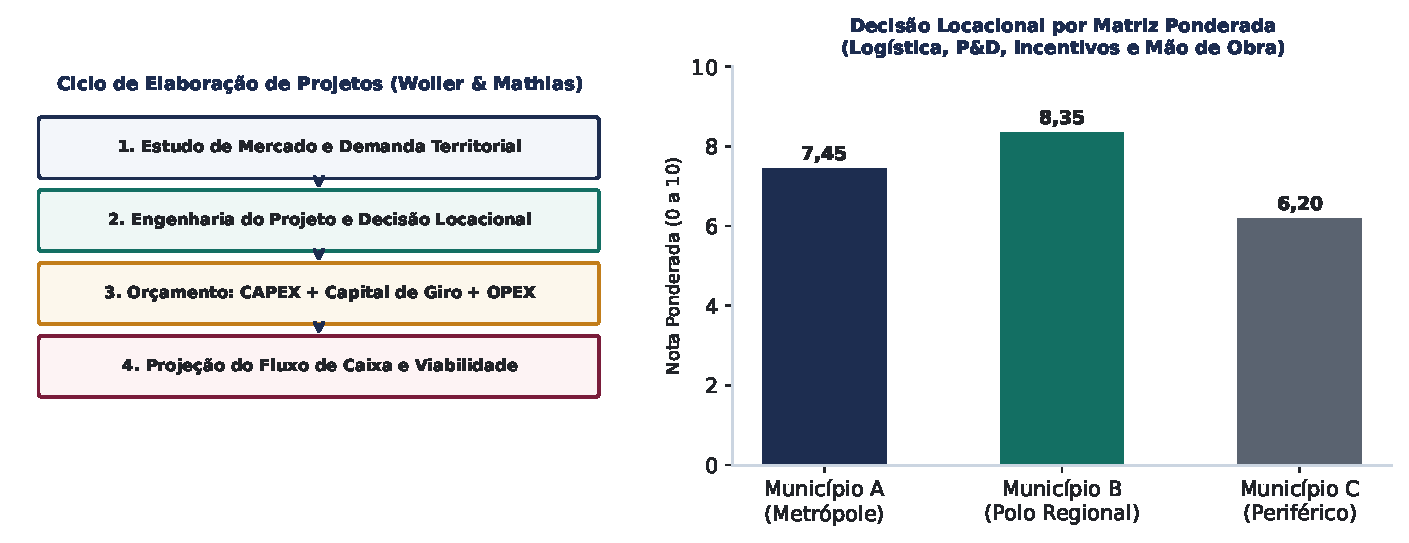
\includegraphics[width=0.95\textwidth]{figures/fig12_ciclo_projetos_localizacao.pdf}
  \caption{Ciclo de elaboração de projetos de investimento, vetores locacionais e integração orçamentária (CAPEX, Capital de Giro e OPEX).}
  \label{fig:12_ciclo}
\end{figure}

\subsection{Matriz Locacional Ponderada}

Quando múltiplos critérios qualitativos e quantitativos competem entre si, o projetista utiliza a \textbf{Matriz Locacional Ponderada} (método de pontuação compensatória). O procedimento exige definir pesos normalizados que reflitam a estratégia do negócio e atribuir notas comparáveis a cada município ou distrito candidato.

\begin{boxFormula}[Matriz Locacional Ponderada]
\[
  Nota_j = \sum_{i=1}^{m} w_i \cdot n_{ij}, \qquad \text{com} \quad \sum_{i=1}^{m} w_i = 1
\]
Para aplicar a matriz com rigor, inicia-se pela definição dos critérios eliminatórios e classificatórios, descartando previamente locais sem licença ambiental viável ou energia mínima exigida. Em seguida, atribuem-se os pesos ($w_i$), distribuindo $1{,}00$ ($100\%$) entre os $m$ critérios conforme o impacto econômico-tecnológico no projeto. Cada localidade $j$ recebe então uma pontuação ($n_{ij}$) em escala uniforme (por exemplo, $0$ a $10$) com base em dados objetivos como tarifas, distância em quilômetros e alíquotas. Multiplica-se $w_i \cdot n_{ij}$ para cada critério e soma-se a coluna da localidade $j$, escolhendo o território de maior $Nota_j$ após verificar a sensibilidade do ranking a pequenas alterações de pesos.
\end{boxFormula}

\subsection{Estrutura Orçamentária: CAPEX, Capital de Giro e OPEX}

Todo projeto de investimento organiza suas saídas de caixa em três grandes blocos que exigem tratamento contábil e financeiro separado. O primeiro bloco é o \textbf{CAPEX (\textit{Capital Expenditure}, ou Investimento Fixo)}, que engloba aquisições de ativos imobilizados e intangíveis de vida útil superior a um ano, tais como terreno, terraplanagem, galpão industrial, máquinas, equipamentos de laboratório, instalações elétricas, veículos utilitários, patentes e softwares corporativos. Esse investimento sofre \textbf{depreciação} (ou amortização) contábil ao longo do tempo e é desembolsado principalmente no Ano $0$ ou em fases programadas de expansão.

O segundo bloco corresponde ao \textbf{Capital de Giro e à Necessidade Líquida de Capital de Giro (NLCG)}, representando o recurso financeiro mantido em circulação para sustentar o descasamento temporal entre pagar fornecedores, estocar insumos, produzir, vender e receber dos clientes. Mesmo um projeto altamente lucrativo perde solvência se falhar no financiamento de seu ciclo financeiro.

O terceiro bloco reúne o \textbf{OPEX (\textit{Operational Expenditure}, ou Custos e Despesas Operacionais)}, composto pelos gastos contínuos do dia a dia para operar a capacidade instalada. Esses gastos dividem-se em \textbf{Custos e Despesas Fixas ($CF$)}, que permanecem constantes diante de variações no volume produzido dentro da faixa de capacidade (aluguel, folha administrativa, depreciação contábil, seguro e vigilância), e \textbf{Custos Variáveis ($CV$)}, que crescem proporcionalmente às unidades produzidas e vendidas (matéria-prima direta, embalagens, energia de processo, comissões e impostos sobre venda).

\begin{boxFormula}[Ciclo Financeiro, NLCG e Ponto de Equilíbrio Contábil]
\textbf{1. Ciclo Financeiro e Necessidade Líquida de Capital de Giro:}
\[
  CF_{ciclo} = PME + PMR - PMP \qquad \Longrightarrow \qquad NLCG = CF_{ciclo} \times \frac{\text{OPEX desembolsável anual}}{360}
\]
onde $PME$ é o prazo médio de estocagem, $PMR$ o prazo médio de recebimento e $PMP$ o prazo médio de pagamento (em dias). Se $CF_{ciclo} > 0$, a empresa precisa financiar $NLCG$ em caixa; se $CF_{ciclo} < 0$, os fornecedores financiam a operação.

\vspace{6pt}
\textbf{2. Ponto de Equilíbrio Contábil ($PE$) e Margem de Segurança ($MS$):}
\[
  PE_{\text{unid}} = \frac{CF}{P - CV_u} = \frac{CF}{MC_u}, \qquad PE_{\text{receita}} = PE_{\text{unid}} \times P, \qquad MS(\%) = \frac{Q_{\text{prevista}} - PE_{\text{unid}}}{Q_{\text{prevista}}} \times 100\%
\]
onde $CF$ são os custos e despesas fixas do período, $P$ o preço unitário de venda, $CV_u$ o custo variável unitário e $MC_u = P - CV_u$ a margem de contribuição unitária. O $PE_{\text{unid}}$ indica o volume mínimo de vendas para que o lucro operacional (LAJIR) seja exatamente zero. Caso haja uma meta de lucro operacional $L_{\text{alvo}}$, soma-se $L_{\text{alvo}}$ ao numerador: $Q_{\text{meta}} = \frac{CF + L_{\text{alvo}}}{P - CV_u}$.
\end{boxFormula}

\etapa{4}{Exemplos Resolvidos Passo a Passo (Padrão de Engenharia Econômica)}

\begin{boxExemplo}{12.1}{Matriz Locacional Ponderada para Agroindústria no Território do Sisal}
\passoEnunciado{Uma cooperativa de inovação rural planeja instalar uma planta de extração de celulose e compósitos a partir de resíduo de sisal. Três municípios baianos foram pré-selecionados: Valente, Conceição do Coité e Feira de Santana.}
\passoDados{Critérios e pesos definidos pela equipe técnica: Proximidade à matéria-prima ($w_1 = 0{,}35$), Disponibilidade de energia e água ($w_2 = 0{,}25$), Infraestrutura logística e acesso a mercados ($w_3 = 0{,}25$) e Incentivos fiscais/terreno municipal ($w_4 = 0{,}15$). As notas técnicas de $0$ a $10$ foram: Valente $[9;\, 8;\, 7;\, 8]$, Conceição do Coité $[7;\, 8;\, 8;\, 7]$ e Feira de Santana $[6;\, 9;\, 9;\, 6]$.}
\passoPedido{Calcular a pontuação ponderada de cada município e indicar a localização recomendada.}
\passoMetodo{Aplicação direta da Matriz Locacional Ponderada: $Nota_j = \sum_{i=1}^{4} w_i \cdot n_{ij}$, verificando antes que $\sum w_i = 0{,}35 + 0{,}25 + 0{,}25 + 0{,}15 = 1{,}00$.}
\passoContas{%
\begin{align*}
  Nota_{\text{Valente}} &= (0{,}35 \times 9) + (0{,}25 \times 8) + (0{,}25 \times 7) + (0{,}15 \times 8) \\
  &= 3{,}15 + 2{,}00 + 1{,}75 + 1{,}20 = 8{,}10 \\[4pt]
  Nota_{\text{Coité}} &= (0{,}35 \times 7) + (0{,}25 \times 8) + (0{,}25 \times 8) + (0{,}15 \times 7) \\
  &= 2{,}45 + 2{,}00 + 2{,}00 + 1{,}05 = 7{,}50 \\[4pt]
  Nota_{\text{Feira}} &= (0{,}35 \times 6) + (0{,}25 \times 9) + (0{,}25 \times 9) + (0{,}15 \times 6) \\
  &= 2{,}10 + 2{,}25 + 2{,}25 + 0{,}90 = 7{,}50
\end{align*}
}
\passoResposta{O município selecionado é \textbf{Valente}, com nota global \textbf{8,10}, superando Conceição do Coité (7,50) e Feira de Santana (7,50) em 0,60 ponto.}
\passoVerificacao{A vantagem de Valente decorre do peso elevado da proximidade à matéria-prima ($35\%$), coerente com o Índice Material de Weber ($IM > 1$) para resíduos agrícolas volumosos: transportar talos e mucilagem bruta por longas distâncias até Feira de Santana destruiria a margem operacional.}
\end{boxExemplo}

\begin{boxExemplo}{12.2}{Dimensionamento de CAPEX Total e Capital de Giro pelo Ciclo Financeiro}
\passoEnunciado{Uma startup de sensores IoT para irrigação localizada no Oeste Baiano (Barreiras) está fechando seu orçamento de implantação para submissão ao FNE Inovação.}
\passoDados{Investimentos fixos previstos: galpão modular e bancadas técnicas \reais{180.000}, equipamentos de soldagem SMD e calibração \reais{220.000}, softwares e registro de firmware \reais{50.000}. Para a operação anual, o OPEX desembolsável projetado é de \reais{720.000}/ano (base comercial de $360$ dias). Os prazos médios negociados são: $PME = 30$ dias, $PMR = 45$ dias e $PMP = 25$ dias.}
\passoPedido{Calcular o CAPEX total, o Ciclo Financeiro ($CF_{ciclo}$), a Necessidade Líquida de Capital de Giro ($NLCG$) e o investimento inicial total requerido no Ano $0$.}
\passoMetodo{Soma dos ativos imobilizados para o CAPEX; cálculo de $CF_{ciclo} = PME + PMR - PMP$; conversão do ciclo em caixa pela taxa diária de desembolso ($\text{OPEX}/360$).}
\passoContas{%
\begin{align*}
  CAPEX &= 180.000 + 220.000 + 50.000 = \reais{450.000} \\[4pt]
  CF_{ciclo} &= 30 + 45 - 25 = 50\text{ dias} \\[4pt]
  \text{Desembolso diário} &= \frac{720.000}{360} = \reais{2.000/\text{dia}} \\[4pt]
  NLCG &= 50 \times 2.000 = \reais{100.000} \\[4pt]
  \text{Investimento Inicial Total} &= CAPEX + NLCG = 450.000 + 100.000 = \reais{550.000}
\end{align*}
}
\passoResposta{CAPEX = \textbf{\reais{450.000}}; Ciclo Financeiro = \textbf{50 dias}; NLCG = \textbf{\reais{100.000}}; Investimento Total no Ano 0 = \textbf{\reais{550.000}}.}
\passoVerificacao{O resultado faz pleno sentido econômico: embora o equipamento custe \reais{450.000}, a startup vende a prazo para produtores rurais ($45$ dias) e mantém estoque de componentes ($30$ dias) pagando fornecedores em $25$ dias, exigindo \reais{100.000} adicionais em caixa para não ficar insolvente nos primeiros meses.}
\end{boxExemplo}

\begin{boxExemplo}{12.3}{Ponto de Equilíbrio Contábil e Margem de Segurança em Bioinsumos}
\passoEnunciado{Uma biofábrica instalada no Recôncavo Baiano (Cruz das Almas) produz inoculantes biológicos líquidos em bombonas de 20 litros para agricultura familiar e médios produtores.}
\passoDados{Custos e despesas fixas anuais ($CF$) = \reais{180.000}; preço de venda por bombona ($P$) = \reais{120,00}; custo variável unitário ($CV_u$, incluindo meio de cultura, embalagem, comissão e imposto sobre venda) = \reais{75,00}; demanda anual contratada ($Q_{\text{prevista}}$) = $5.000$ bombonas.}
\passoPedido{Determinar a margem de contribuição unitária ($MC_u$), o Ponto de Equilíbrio em unidades ($PE_{\text{unid}}$) e em receita ($PE_{\text{receita}}$), além da Margem de Segurança ($MS$).}
\passoMetodo{Aplicação das equações de equilíbrio linear: $MC_u = P - CV_u$, $PE_{\text{unid}} = CF / MC_u$ e $MS = (Q_{\text{prevista}} - PE_{\text{unid}}) / Q_{\text{prevista}}$.}
\passoContas{%
\begin{align*}
  MC_u &= 120{,}00 - 75{,}00 = \reais{45{,}00/\text{bombona}} \\[4pt]
  PE_{\text{unid}} &= \frac{180.000}{45{,}00} = 4.000\text{ bombonas/ano} \\[4pt]
  PE_{\text{receita}} &= 4.000 \times 120{,}00 = \reais{480.000/\text{ano}} \\[4pt]
  MS(\%) &= \frac{5.000 - 4.000}{5.000} \times 100\% = \frac{1.000}{5.000} \times 100\% = 20\%
\end{align*}
}
\passoResposta{$MC_u = \mathbf{\reais{45{,}00}}$; $PE_{\text{unid}} = \mathbf{4.000\text{ bombonas}}$; $PE_{\text{receita}} = \mathbf{\reais{480.000}}$; Margem de Segurança = \textbf{20\%}.}
\passoVerificacao{Uma margem de segurança de $20\%$ indica que as vendas podem cair até $1.000$ bombonas abaixo do planejado antes que a biofábrica entre em prejuízo operacional. Esse colchão de segurança é coerente para agroindústrias expostas à sazonalidade climática.}
\end{boxExemplo}

\begin{boxExemplo}{12.4}{Orientação Locacional de Weber e Índice Material}
\passoEnunciado{Uma cooperativa de agricultores analisa onde instalar uma unidade de processamento de mandioca para produção de fécula seca: junto à zona produtora rural (Fonte), no meio do caminho (Entroncamento) ou na capital consumidora (Mercado).}
\passoDados{Para produzir $250\text{ t/ano}$ de fécula (produto acabado, PA), são necessárias $1.000\text{ t/ano}$ de raiz de mandioca bruta (matéria-prima, MP). A distância entre a fonte de MP e o mercado consumidor é de $100\text{ km}$. O frete rodoviário da MP custa \reais{2{,}00}$/(\text{t}\cdot\text{km})$ e o frete do PA custa \reais{3{,}00}$/(\text{t}\cdot\text{km})$.}
\passoPedido{Calcular o Índice Material ($IM$) de Weber e o custo total anual de transporte ($CT$) para as três localizações: na Fonte ($d_{MP}=0$, $d_{PA}=100$), no Entroncamento ($d_{MP}=50$, $d_{PA}=50$) e no Mercado ($d_{MP}=100$, $d_{PA}=0$).}
\passoMetodo{Cálculo de $IM = \text{Peso}_{MP} / \text{Peso}_{PA}$ e da função linear de custo de transporte $CT = Q_{MP} \cdot t_{MP} \cdot d_{MP} + Q_{PA} \cdot t_{PA} \cdot d_{PA}$.}
\passoContas{%
\begin{align*}
  IM &= \frac{1.000}{250} = 4{,}0 \quad (\text{perda de } 75\% \text{ de massa em água e casca}) \\[4pt]
  CT_{\text{Fonte}} &= (1.000 \times 2{,}00 \times 0) + (250 \times 3{,}00 \times 100) = 0 + 75.000 = \reais{75.000/\text{ano}} \\[4pt]
  CT_{\text{Entroncamento}} &= (1.000 \times 2{,}00 \times 50) + (250 \times 3{,}00 \times 50) = 100.000 + 37.500 = \reais{137.500/\text{ano}} \\[4pt]
  CT_{\text{Mercado}} &= (1.000 \times 2{,}00 \times 100) + (250 \times 3{,}00 \times 0) = 200.000 + 0 = \reais{200.000/\text{ano}}
\end{align*}
}
\passoResposta{$IM = \mathbf{4{,}0}$; a localização de menor custo de transporte é \textbf{na Fonte de matéria-prima} (\reais{75.000/ano}), gerando economia anual de \reais{125.000} em relação ao Mercado.}
\passoVerificacao{Mesmo com o frete unitário do produto acabado sendo $50\%$ mais caro que o da matéria-prima (\reais{3{,}00} contra \reais{2{,}00}), a redução de massa de $4$ para $1$ no beneficiamento torna economicamente irracional transportar água e resíduos brutos até a capital. Isso fundamenta a agroindustrialização descentralizada no interior.}
\end{boxExemplo}

\begin{boxExemplo}{12.5}{Análise de Trade-off: Incentivo Fiscal Territorial versus Custo Variável de Frete}
\passoEnunciado{Uma empresa de embalagens biodegradáveis avalia transferir sua planta da região metropolitana para um município do interior que oferece incentivos fiscais e fundiários, porém aumenta o custo de frete de entrega.}
\passoDados{Cenário Base (metropolitano): $CF = \reais{240.000/\text{ano}}$, $P = \reais{200{,}00/\text{unidade}}$ e $CV_u = \reais{120{,}00/\text{unidade}}$. Cenário Interior: cessão de galpão e isenção de taxas locais reduzem $CF$ em $25\%$, mas o frete adicional eleva $CV_u$ para \reais{128{,}00/\text{unidade}}.}
\passoPedido{Comparar o Ponto de Equilíbrio Contábil antes e depois da mudança locacional e avaliar se a transferência reduz o risco operacional.}
\passoMetodo{Cálculo de $PE_{\text{base}}$ e $PE_{\text{interior}}$ após atualização de $CF' = 0{,}75 \times CF$ e $CV_u' = 128{,}00$.}
\passoContas{%
\begin{align*}
  \text{Cenário Base:} \quad MC_u &= 200{,}00 - 120{,}00 = \reais{80{,}00}, \qquad PE_{\text{base}} = \frac{240.000}{80{,}00} = 3.000\text{ unidades} \\[6pt]
  \text{Cenário Interior:} \quad CF' &= 240.000 \times (1 - 0{,}25) = \reais{180.000} \\
  MC_u' &= 200{,}00 - 128{,}00 = \reais{72{,}00} \\
  PE_{\text{interior}} &= \frac{180.000}{72{,}00} = 2.500\text{ unidades}
\end{align*}
}
\passoResposta{O Ponto de Equilíbrio cai de \textbf{3.000 para 2.500 unidades/ano} (redução de $500$ unidades ou $16{,}7\%$), diminuindo o risco de prejuízo em cenários de baixa demanda.}
\passoVerificacao{O incentivo territorial compensa o frete adicional porque a redução de $25\%$ no custo fixo supera a perda de $10\%$ na margem de contribuição unitária. Acima de $7.500$ unidades ($60.000 / 8{,}00$), porém, o custo variável maior faria o cenário metropolitano gerar lucro total superior, evidenciando que a decisão depende da escala esperada.}
\end{boxExemplo}

\etapa{5}{Armadilhas Conceituais e Erros Mais Comuns}

\begin{boxErro}[Erro 1: Somar CAPEX e OPEX como se fossem despesas do mesmo período]
Incluir o valor integral de compra de máquinas (\reais{400.000} de CAPEX) dentro do custo fixo anual do Ponto de Equilíbrio distorce o cálculo, elevando artificialmente o $PE$. O ativo imobilizado entra no custo contábil anual apenas via \textbf{depreciação} (ou é tratado integralmente como investimento no Ano $0$ do Fluxo de Caixa Livre).
\end{boxErro}

\begin{boxErro}[Erro 2: Esquecer o Capital de Giro (NLCG) no investimento inicial]
Projetar apenas terrenos e máquinas e ignorar que a empresa precisa financiar estoques ($PME$) e vendas a prazo ($PMR$) leva à quebra de liquidez nos primeiros meses de operação, mesmo quando o produto tem boa margem de contribuição.
\end{boxErro}

\begin{boxErro}[Erro 3: Pesos não normalizados ou critérios redundantes na Matriz Locacional]
Atribuir pesos que não somam $1{,}00$ (ou $100\%$) ou duplicar o mesmo fator sob dois nomes diferentes (ex.: ``proximidade à rodovia'' e ``acesso rodoviário'') infla artificialmente um critério e invalida a comparação entre municípios.
\end{boxErro}

\begin{boxErro}[Erro 4: Confundir Ponto de Equilíbrio Contábil com Viabilidade Econômica]
Atingir o $PE_{\text{unid}}$ significa apenas que o lucro contábil operacional é zero, não que o projeto remunera o capital investido (TMA). Um projeto pode operar acima do Ponto de Equilíbrio e ainda assim destruir valor econômico se o retorno não superar o custo de oportunidade (Cap. 13).
\end{boxErro}

\etapa{6}{Lista de Exercícios de Fixação (15 Questões)}

\begin{enumerate}[leftmargin=1.6em, itemsep=5pt]
  \item Explique a diferença funcional entre estudo de pré-viabilidade, EVTE (anteprojeto) e projeto executivo segundo Woiler e Mathias (2008). \espacoResolucao[1.5cm]
  \item Por que uma agroindústria de processamento de polpa de frutas ou sisal tende a se localizar próxima à zona produtora, enquanto uma engarrafadora de refrigerantes tende a se localizar próxima ao mercado urbano? Utilize o conceito de Índice Material ($IM$) de Weber. \espacoResolucao[1.5cm]
  \item Uma empresa avalia dois municípios ($A$ e $B$) usando três critérios com pesos $w = [0{,}40;\, 0{,}30;\, 0{,}30]$. O Município $A$ obteve notas $[8;\, 7;\, 9]$ e o Município $B$ obteve $[9;\, 8;\, 6]$. Calcule as notas ponderadas e indique o vencedor. \espacoResolucao[1.6cm]
  \item Uma unidade de beneficiamento processa $500\text{ t/ano}$ de matéria-prima bruta para gerar $100\text{ t/ano}$ de produto acabado ($IM = 5$). A distância entre a fonte e o mercado é de $80\text{ km}$. O frete da MP custa \reais{1{,}50}$/(\text{t}\cdot\text{km})$ e o do PA custa \reais{2{,}50}$/(\text{t}\cdot\text{km})$. Compare o custo anual de transporte na Fonte versus no Mercado. \espacoResolucao[1.8cm]
  \item Calcule a Necessidade Líquida de Capital de Giro ($NLCG$) de uma startup cujo $PME = 40$ dias, $PMR = 35$ dias, $PMP = 30$ dias e o OPEX desembolsável anual é de \reais{1.080.000} (ano comercial de $360$ dias). \espacoResolucao[1.6cm]
  \item Classifique os seguintes itens em \textbf{CAPEX} ou \textbf{OPEX}: (a) aquisição de espectrofotômetro; (b) energia elétrica mensal da fábrica; (c) obras de fundação do galpão; (d) salários da equipe de vendas; (e) compra de licença perpétua de software CAD. \espacoResolucao[1.5cm]
  \item Calcule o CAPEX total de um laboratório de biotecnologia que prevê: terreno \reais{120.000}, obras civis \reais{280.000}, máquinas e biorreatores \reais{350.000} e softwares imobilizados \reais{50.000}. \espacoResolucao[1.4cm]
  \item Uma fábrica de sensores ambientais possui $CF = \reais{150.000/\text{ano}}$, preço unitário $P = \reais{90{,}00}$ e custo variável unitário $CV_u = \reais{40{,}00}$. Calcule o Ponto de Equilíbrio em unidades e em receita anual. \espacoResolucao[1.6cm]
  \item Considerando um projeto com $CF = \reais{120.000/\text{ano}}$, $P = \reais{100{,}00}$ e $CV_u = \reais{60{,}00}$, quantas unidades devem ser vendidas para atingir um lucro operacional alvo de \reais{40.000/\text{ano}}? \espacoResolucao[1.6cm]
  \item Se as vendas previstas de um empreendimento são de $5.000$ unidades/ano e seu Ponto de Equilíbrio Contábil é de $3.500$ unidades/ano, qual é a Margem de Segurança percentual e o que ela significa na gestão de risco? \espacoResolucao[1.5cm]
  \item Uma cooperativa produz $2.000$ unidades/ano com custos fixos de \reais{80.000/\text{ano}} e custo variável unitário de \reais{30{,}00}. Qual é o OPEX total anual e qual é o custo unitário total por unidade produzida? \espacoResolucao[1.5cm]
  \item Três cidades ($X, Y, Z$) concorrem para abrigar um centro de P\&D com pesos $w = [0{,}30;\, 0{,}40;\, 0{,}30]$ (Talentos, Infraestrutura, Incentivos). As notas são: $X=[7;\, 9;\, 6]$, $Y=[8;\, 8;\, 7]$ e $Z=[9;\, 6;\, 8]$. Calcule a pontuação de cada cidade. \espacoResolucao[1.8cm]
  \item O que ocorre com a Necessidade Líquida de Capital de Giro quando uma empresa digital apresenta $PME = 15$ dias, $PMR = 10$ dias e $PMP = 45$ dias? Calcule o Ciclo Financeiro e interprete. \espacoResolucao[1.5cm]
  \item Explique como a presença de uma universidade ou instituto de pesquisa (fator P\&D) e de um APL (economias externas) altera a Matriz Locacional de uma startup de base tecnológica em comparação com uma indústria tradicional. \espacoResolucao[1.5cm]
  \item Por que incentivos fiscais isolados (como redução temporária de ICMS) podem gerar armadilhas locacionais caso o território não possua infraestrutura logística nem capital humano compatíveis com o projeto? \espacoResolucao[1.5cm]
\end{enumerate}

\etapa{7}{Desafios Autorais e Aplicação Territorial (Preparação AV3)}

\begin{enumerate}[leftmargin=1.6em, itemsep=5pt]
  \item \textbf{Projeto Territorial Aplicado:} Escolha o território onde seu grupo desenvolve o projeto da AV3. Defina $4$ critérios locacionais relevantes (com pesos somando $1{,}00$) e compare dois municípios candidatos com justificativa técnica das notas atribuídas. \espacoResolucao[1.8cm]
  \item \textbf{Orçamento Mínimo Viável:} Liste os $5$ principais itens de CAPEX e os $4$ principais itens de OPEX do seu projeto da AV3, identificando qual linha de fomento (BNDES, FINEP, BNB/FNE ou FAPESB) seria mais aderente ao financiamento do CAPEX. \espacoResolucao[1.8cm]
  \item \textbf{Análise Crítica de Risco Operacional:} Explique como uma redução de $15\%$ no preço de venda praticado no mercado afetaria o Ponto de Equilíbrio Contábil de um empreendimento com alta proporção de custos fixos (alavancagem operacional elevada). \espacoResolucao[1.6cm]
\end{enumerate}

\begin{boxDica}[Contraponto Crítico e Prática Territorial (AV2 e AV3)]
Na defesa oral da AV3, a banca avalia se o orçamento do projeto conversa com a realidade do território. Não basta apresentar um CAPEX genérico: demonstre de onde vêm as cotações de equipamentos, justifique a necessidade de capital de giro pelo prazo real de pagamento das cadeias locais (agricultura familiar, cooperativas ou editais públicos costumam ter $PMR$ elevado) e evidencie por que a localização escolhida maximiza o valor líquido do empreendimento.
\end{boxDica}

\clearpage
\etapa{8}{Gabarito Integralmente Comentado (Exercícios 1 a 15 + Desafios 1 a 3)}

\begin{boxGabarito}[Resolução Passo a Passo: Exercícios de Fixação (1 a 15)]
\begin{enumerate}[leftmargin=1.5em, itemsep=4pt]
  \item \textbf{Estágios do projeto:} O estudo de pré-viabilidade testa a ideia preliminarmente para descartar inviabilidades óbvias a baixo custo; o EVTE (anteprojeto) quantifica mercado, tecnologia, localização, CAPEX, giro, OPEX e retorno financeiro; o projeto executivo detalha plantas e especificações finais para execução de obra e financiamento.
  \item \textbf{Weber ($IM$):} Na polpa de frutas ou sisal, perde-se grande massa em casca, água e resíduos ($IM > 1$), logo o frete da matéria-prima bruta pesa mais e atrai a planta para a fonte rural. No refrigerante, transporta-se xarope concentrado e adiciona-se água local no destino ($IM < 1$), atraindo a fábrica para o mercado urbano.
  \item \textbf{Matriz Locacional:}
  $Nota_A = 0{,}40(8) + 0{,}30(7) + 0{,}30(9) = 3{,}20 + 2{,}10 + 2{,}70 = \mathbf{8{,}00}$. \\
  $Nota_B = 0{,}40(9) + 0{,}30(8) + 0{,}30(6) = 3{,}60 + 2{,}40 + 1{,}80 = \mathbf{7{,}80}$. \\
  Vencedor: \textbf{Município A} (8,00 pontos).
  \item \textbf{Transporte (Weber):}
  Na Fonte ($d_{MP}=0, d_{PA}=80$): $CT_{\text{Fonte}} = 100 \times 2{,}50 \times 80 = \mathbf{\reais{20.000/\text{ano}}}$. \\
  No Mercado ($d_{MP}=80, d_{PA}=0$): $CT_{\text{Mercado}} = 500 \times 1{,}50 \times 80 = \mathbf{\reais{60.000/\text{ano}}}$. \\
  Economia de \reais{40.000/ano} ao localizar na Fonte.
  \item \textbf{NLCG:} $CF_{ciclo} = 40 + 35 - 30 = 45\text{ dias}$. Desembolso diário $= 1.080.000 / 360 = \reais{3.000/\text{dia}}$. Logo, $NLCG = 45 \times 3.000 = \mathbf{\reais{135.000}}$.
  \item \textbf{Classificação:} (a) CAPEX; (b) OPEX; (c) CAPEX; (d) OPEX; (e) CAPEX.
  \item \textbf{CAPEX total:} $120.000 + 280.000 + 350.000 + 50.000 = \mathbf{\reais{800.000}}$.
  \item \textbf{Ponto de Equilíbrio:} $MC_u = 90 - 40 = \reais{50{,}00}$. $PE_{\text{unid}} = 150.000 / 50 = \mathbf{3.000\text{ unidades}}$. $PE_{\text{receita}} = 3.000 \times 90 = \mathbf{\reais{270.000}}$.
  \item \textbf{PE com lucro alvo:} $MC_u = 100 - 60 = \reais{40{,}00}$. $Q_{\text{meta}} = (120.000 + 40.000) / 40 = 160.000 / 40 = \mathbf{4.000\text{ unidades}}$.
  \item \textbf{Margem de Segurança:} $MS = (5.000 - 3.500) / 5.000 = 1.500 / 5.000 = \mathbf{30\%}$. As vendas podem recuar até $30\%$ antes de haver prejuízo operacional.
  \item \textbf{OPEX e custo unitário:} $OPEX = 80.000 + (2.000 \times 30) = 80.000 + 60.000 = \mathbf{\reais{140.000/\text{ano}}}$. Custo unitário total $= 140.000 / 2.000 = \mathbf{\reais{70{,}00/\text{unidade}}}$.
  \item \textbf{Matriz 3 cidades:}
  $Nota_X = 0{,}3(7) + 0{,}4(9) + 0{,}3(6) = 2{,}1 + 3{,}6 + 1{,}8 = \mathbf{7{,}50}$. \\
  $Nota_Y = 0{,}3(8) + 0{,}4(8) + 0{,}3(7) = 2{,}4 + 3{,}2 + 2{,}1 = \mathbf{7{,}70}$. \\
  $Nota_Z = 0{,}3(9) + 0{,}4(6) + 0{,}3(8) = 2{,}7 + 2{,}4 + 2{,}4 = \mathbf{7{,}50}$. \\
  Vencedora: \textbf{Cidade Y} (7,70 pontos).
  \item \textbf{Ciclo Financeiro negativo:} $CF_{ciclo} = 15 + 10 - 45 = \mathbf{-20\text{ dias}}$. A empresa recebe dos clientes antes de pagar os fornecedores, gerando folga de caixa (capital de giro negativo) em vez de exigir imobilização financeira.
  \item \textbf{P\&D e APL:} Em startups tecnológicas, o custo de transporte físico pesa menos que o acesso a pesquisadores, laboratórios compartilhados e fluxos de conhecimento tácito; assim, os pesos de P\&D e aglomeração superam o peso tradicional do frete.
  \item \textbf{Armadilha fiscal:} Benefícios fiscais têm prazo determinado e não corrigem gargalos estruturais de estradas, falta de energia confiável ou escassez de técnicos; quando o incentivo expira, a operação torna-se antieconômica.
\end{enumerate}
\end{boxGabarito}

\begin{boxGabarito}[Diretrizes de Resposta: Desafios Autorais (1 a 3)]
\begin{enumerate}[leftmargin=1.5em, itemsep=3pt]
  \item \textbf{Desafio 1:} Deve apresentar matriz com $\sum w_i = 1{,}00$, notas justificadas por dados verificáveis (distância em km, tarifa elétrica, presença de ICTs) e conclusão coerente com a maior pontuação ponderada.
  \item \textbf{Desafio 2:} Deve separar claramente imobilizações (CAPEX) de gastos recorrentes (OPEX) e associar equipamentos/obras a linhas como BNDES Automático ou BNB/FNE e P\&D a subvenção/crédito FINEP ou FAPESB.
  \item \textbf{Desafio 3:} Uma queda de $15\%$ no preço reduz diretamente a margem de contribuição unitária ($MC_u = P - CV_u$) em proporção maior que $15\%$, elevando fortemente o $PE_{\text{unid}}$. Em estruturas com $CF$ alto, pequenas quedas de preço comprimem o lucro rapidamente.
\end{enumerate}
\end{boxGabarito}

\begin{boxResumo}
\begin{itemize}[leftmargin=1.4em, itemsep=2pt]
  \item Projetos executivos amadurecem da pré-viabilidade ao EVTE e ao projeto final (Woiler \& Mathias, 2008).
  \item A decisão locacional integra custos de transporte (Weber/Von Thünen), infraestrutura, P\&D e incentivos via \textbf{Matriz Locacional Ponderada} ($Nota_j = \sum w_i \cdot n_{ij}$).
  \item O orçamento separa investimento fixo (\textbf{CAPEX}), Necessidade Líquida de Capital de Giro ($NLCG = CF_{ciclo} \times \text{OPEX}/360$) e gastos contínuos (\textbf{OPEX}).
  \item O Ponto de Equilíbrio Contábil ($PE = CF / (P - CV_u)$) mede o volume mínimo para zerar o prejuízo operacional, mas não substitui a análise de viabilidade intertemporal.
\end{itemize}
\end{boxResumo}

\begin{boxTeste}
\begin{enumerate}[leftmargin=1.5em, itemsep=4pt]
  \item Uma startup tem $CF = \reais{96.000/\text{ano}}$, $P = \reais{80{,}00}$ e $CV_u = \reais{56{,}00}$. Qual é o Ponto de Equilíbrio Contábil em unidades?
  \item Na Matriz Locacional com pesos $[0{,}50;\, 0{,}30;\, 0{,}20]$, uma cidade recebe notas $[8;\, 6;\, 9]$. Qual é sua nota final?
  \item (\V/\F) Na teoria de Weber, processos industriais com grande perda de massa ($IM > 1$) tendem a se localizar junto ao mercado consumidor.
  \item (\V/\F) Um Ciclo Financeiro positivo ($PME + PMR > PMP$) exige aporte de Capital de Giro no início do projeto.
\end{enumerate}
\vspace{4pt}
\noindent\textbf{Gabarito do Checkpoint:} \textbf{1.} $MC_u = 80 - 56 = \reais{24{,}00} \Rightarrow PE = 96.000 / 24 = \mathbf{4.000\text{ unidades}}$. \quad \textbf{2.} $0{,}5(8) + 0{,}3(6) + 0{,}2(9) = 4{,}0 + 1{,}8 + 1{,}8 = \mathbf{7{,}60}$. \quad \textbf{3.} \F\ (tendem a se localizar junto à fonte de matéria-prima). \quad \textbf{4.} \V.
\end{boxTeste}

\chapter{Métodos e Ferramentas para Análise de Investimentos}
\label{cap:13}

\noindent\tagAV{AV2 (20\%)}\ \tagQuant
\vspace{6pt}

\begin{capObjetivos}
Ao concluir este capítulo, você será capaz de:
\begin{enumerate}[leftmargin=1.4em, itemsep=2pt]
  \item Aplicar o princípio do valor do dinheiro no tempo por meio de juros compostos, desconto intertemporal e definição da Taxa Mínima de Atratividade (\textbf{TMA}) como custo de oportunidade.
  \item Construir passo a passo o \textbf{Fluxo de Caixa Livre (FCL)} a partir de receitas, OPEX, depreciação, imposto de renda, variação de capital de giro e CAPEX.
  \item Calcular, interpretar e decidir com base nos principais indicadores de viabilidade: \textbf{VPL}, \textbf{TIR} (reconhecendo múltiplas TIRs e a hipótese de reinvestimento), \textbf{MTIR}, \textbf{VAUE} (para projetos com vidas úteis distintas), \textbf{Payback Simples} e \textbf{Payback Descontado}.
  \item Conduzir análises de sensibilidade e cenários (otimista, base e pessimista) para avaliar a robustez de projetos tecnológicos e territoriais.
\end{enumerate}
\end{capObjetivos}

\begin{capRevisao}
Antes de modelar os fluxos descontados, retome três conceitos do Capítulo 12:
\begin{itemize}[leftmargin=1.4em, itemsep=2pt]
  \item \textbf{CAPEX versus OPEX:} o investimento fixo ocorre no Ano $0$ (ou em expansões pontuais) e é recuperado economicamente ao longo da vida útil, enquanto o OPEX se repete a cada período operacional.
  \item \textbf{Capital de Giro ($NLCG$):} variações positivas na necessidade de giro consomem caixa no período em que ocorrem e são recuperadas ao final do horizonte do projeto.
  \item \textbf{Limitação do Ponto de Equilíbrio:} o equilíbrio contábil anual não incorpora o custo de oportunidade do capital imobilizado nem a distribuição dos fluxos ao longo dos anos.
\end{itemize}
\end{capRevisao}

\etapa{3}{Valor do Dinheiro no Tempo, Fluxo de Caixa Livre e Indicadores}

\subsection{Valor do dinheiro no tempo e Taxa Mínima de Atratividade (TMA)}

Um real recebido hoje vale mais do que um real a ser recebido daqui a um ano por três razões objetivas: \textbf{custo de oportunidade} (o capital disponível hoje pode render juros em aplicações alternativas), \textbf{inflação} (perda de poder de compra) e \textbf{risco} (incerteza quanto ao recebimento futuro). No regime de juros compostos, um Valor Presente ($VP$) capitalizado à taxa $i$ por $t$ períodos gera um Valor Futuro $VF = VP \cdot (1 + i)^t$; inversamente, trazer um fluxo futuro $FC_t$ para a data zero exige dividi-lo pelo fator $(1 + TMA)^t$.

A \textbf{Taxa Mínima de Atratividade (TMA)} é a taxa de retorno mínima que o investidor ou empreendedor exige para aceitar o projeto, equivalente ao rendimento da melhor alternativa disponível de risco comparável (custo de oportunidade do capital).

\begin{boxSimbolo}[Vocabulário Conceitual e Símbolos do Capítulo 13]
Na modelagem intertemporal, $FC_t$ ou $FCL_t$ indica o Fluxo de Caixa Livre no período $t$ ($t = 0, 1, \dots, n$), descontado pela Taxa Mínima de Atratividade ($TMA$, expressa em decimal, como $0{,}12$ para $12\%$ a.a.). A criação absoluta de riqueza em moeda presente é medida pelo Valor Presente Líquido ($VPL$, em \reais{}), complementado pelo Índice de Lucratividade ($IL$).

Entre os indicadores de taxa e prazo, $TIR$ designa a Taxa Interna de Retorno que anula o VPL, enquanto $MTIR$ representa a Taxa Interna de Retorno Modificada, calculada com taxa de financiamento $k_f$ e taxa de reinvestimento $k_r$. Por meio do Fator de Recuperação de Capital $FRC(i,n)$, o Valor Anual Uniforme Equivalente ($VAUE$) permite comparar alternativas de durações distintas. O tempo de recuperação do capital é aferido pelo Payback Simples ($PBS$) e pelo Payback Descontado ($PBD$, em anos ou períodos), ao passo que a apuração do fluxo parte do Lucro Antes do Imposto de Renda ($LAIR$), da Depreciação contábil ($Depr$) e da Variação de Capital de Giro ($\Delta CG$).
\end{boxSimbolo}

\subsection{Construção do Fluxo de Caixa Livre (FCL)}

A análise de investimentos utiliza \textbf{caixa efetivo}, nunca apenas lucro contábil. Como a depreciação reduz o lucro tributável sem representar saída de dinheiro do caixa, ela é subtraída para calcular o imposto de renda e somada de volta após o imposto.

\begin{boxFormula}[Estrutura Padrão do Fluxo de Caixa Livre ($FCL_t$)]
\begin{align*}
  \text{LAIR}_t &= \text{Receita}_t - \text{OPEX}_{\text{desembolsável}, t} - \text{Depreciação}_t \\
  \text{Lucro Líquido}_t &= \text{LAIR}_t \times (1 - T_{\text{IR/CSLL}}) \\
  \text{FCO}_t &= \text{Lucro Líquido}_t + \text{Depreciação}_t \\
  \text{FCL}_t &= \text{FCO}_t - \Delta \text{CG}_t - \text{CAPEX}_t + \text{Valor Residual líquido}_t
\end{align*}
No Ano $0$, geralmente $\text{FCL}_0 = -\text{CAPEX}_0 - \text{CG}_0$. Ao final do horizonte $n$, o capital de giro acumulado é recuperado ($\Delta \text{CG}_n < 0$, somando caixa).
\end{boxFormula}

\subsection{Métodos de Análise de Investimentos}

\begin{boxFormula}[VPL, TIR, MTIR, VAUE e Payback]
\textbf{1. Valor Presente Líquido (VPL):} origem na matemática financeira de Irving Fisher (1930); mede a riqueza líquida absoluta criada pelo projeto em moeda de hoje.
\[
  VPL = \sum_{t=0}^{n} \frac{FCL_t}{(1 + TMA)^t} = FCL_0 + \frac{FCL_1}{(1+TMA)^1} + \dots + \frac{FCL_n}{(1+TMA)^n}
\]
\textit{Critério de decisão:} aceitar se $VPL > 0$; rejeitar se $VPL < 0$; indiferente se $VPL = 0$. Entre projetos mutuamente excludentes de mesma duração, escolher o de maior $VPL$. O Índice de Lucratividade complementar é $IL = \frac{\sum_{t=1}^{n} FCL_t/(1+TMA)^t}{|FCL_0|}$ (aceitar se $IL > 1$).

\vspace{5pt}
\textbf{2. Taxa Interna de Retorno (TIR):} taxa de desconto $r^*$ que iguala o VPL a zero:
\[
  \sum_{t=0}^{n} \frac{FCL_t}{(1 + TIR)^t} = 0
\]
\textit{Critério de decisão:} para projetos convencionais (um sinal negativo em $t=0$ seguido de positivos), aceitar se $TIR > TMA$. Dois problemas críticos limitam esse indicador. Em fluxos não convencionais, com múltiplas inversões de sinal (como descomissionamento ambiental no último ano), a equação polinomial gera \textbf{múltiplas TIRs} ou nenhuma raiz real (Regra dos Sinais de Descartes); além disso, a TIR pressupõe implicitamente que os fluxos intermediários positivos são reinvestidos à própria $TIR$, o que é irrealista quando a $TIR$ é muito superior à taxa de mercado.

\vspace{5pt}
\textbf{3. Taxa Interna de Retorno Modificada (MTIR):} corrige o pressuposto irrealista de reinvestimento da TIR descontando os fluxos negativos à taxa de financiamento ($k_f$) até $t=0$ e capitalizando os fluxos positivos à taxa de reinvestimento ($k_r$, geralmente a $TMA$) até $t=n$:
\[
  MTIR = \left( \frac{\sum_{t: FCL_t > 0} FCL_t (1 + k_r)^{n-t}}{\sum_{t: FCL_t < 0} \frac{|FCL_t|}{(1 + k_f)^t}} \right)^{\frac{1}{n}} - 1
\]
\textit{Critério de decisão:} aceitar se $MTIR > TMA$. Garante solução única mesmo com múltiplos fluxos negativos.

\vspace{5pt}
\textbf{4. Valor Anual Uniforme Equivalente (VAUE):} indispensável para comparar projetos mutuamente excludentes com \textbf{vidas úteis diferentes} ($n_A \neq n_B$), pois converte o VPL total em uma série uniforme anual equivalente:
\[
  VAUE = VPL \times FRC(TMA, n), \qquad \text{onde} \quad FRC(i, n) = \frac{i(1+i)^n}{(1+i)^n - 1}
\]
\textit{Critério de decisão:} entre alternativas de durações distintas com possibilidade de renovação, escolher o projeto de maior $VAUE$ positivo.

\vspace{5pt}
\textbf{5. Payback Simples ($PBS$) e Payback Descontado ($PBD$):} medem o tempo necessário para recuperar o investimento inicial. O $PBS$ soma fluxos nominais (ignorando o valor do dinheiro no tempo); o $PBD$ soma os fluxos já trazidos a valor presente pela $TMA$. Se a recuperação ocorrer entre os anos $k$ e $k+1$:
\[
  PBD = k + \frac{|\text{Saldo Descontado Acumulado}_{k}|}{VP(FCL_{k+1})}
\]
\end{boxFormula}

A Figura~\ref{fig:13_perfil} ilustra o comportamento do Valor Presente Líquido em função da taxa de desconto, evidenciando o ponto em que a curva cruza o eixo horizontal (a própria TIR) e permitindo comparar projetos mutuamente excludentes sob diferentes custos de oportunidade.

\begin{figure}[H]
  \centering
  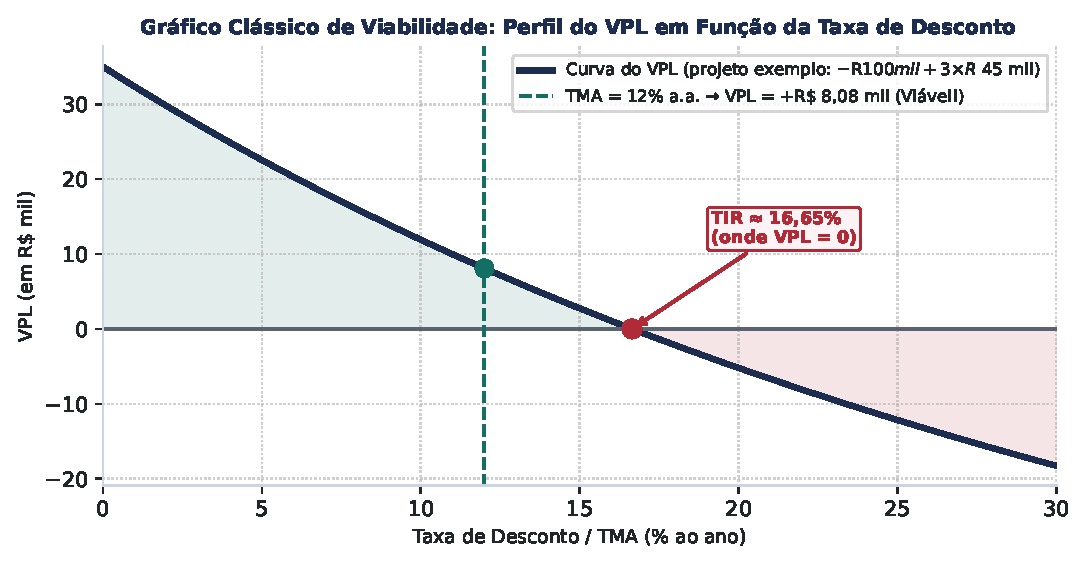
\includegraphics[width=0.88\textwidth]{figures/fig13_perfil_vpl_tir.pdf}
  \caption{Perfil do Valor Presente Líquido (VPL) em função da taxa de desconto, interseção com a TIR e comparação de projetos.}
  \label{fig:13_perfil}
\end{figure}

\subsection{Análise de sensibilidade e cenários}

Como projeções financeiras contêm incerteza quanto a preços, custos e demanda territorial, avalia-se a robustez do VPL por dois caminhos complementares. Na \textbf{Análise de Sensibilidade (univariada)}, você varia uma única premissa por vez, mantendo as demais constantes (por exemplo, preço em $-10\%$, OPEX em $+15\%$ ou $TMA$ oscilando de $8\%$ a $16\%$), para identificar qual variável exerce maior impacto sobre a viabilidade do projeto. Já na \textbf{Análise de Cenários (multivariada)}, definem-se estados macroeconômicos e territoriais consistentes (\textit{Pessimista}, \textit{Base} e \textit{Otimista}) com probabilidades atribuídas $p_s$ ($\sum p_s = 1$), calculando-se o VPL esperado pela média ponderada $\mathbb{E}[VPL] = \sum_s p_s \cdot VPL_s$.

\etapa{4}{Exemplos Resolvidos Passo a Passo}

\begin{boxExemplo}{13.1}{Construção Completa do Fluxo de Caixa Livre (FCL)}
\passoEnunciado{Uma empresa de tecnologia limpa implanta um biodigestor modular para agroindústria regional com horizonte de $3$ anos.}
\passoDados{Ano $0$: CAPEX = \reais{300.000} (depreciação linear em $3$ anos, sem valor residual) e capital de giro inicial ($CG_0$) = \reais{40.000}. Anos $1$ a $3$: Receita anual = \reais{250.000}; OPEX desembolsável anual = \reais{110.000}; alíquota de IR/CSLL = $34\%$. No Ano $1$, há reforço adicional de capital de giro ($\Delta CG_1 = +\reais{10.000}$); no Ano $2$, $\Delta CG_2 = 0$; no Ano $3$, todo o capital de giro acumulado (\reais{50.000}) é recuperado ($\Delta CG_3 = -\reais{50.000}$). $TMA = 10\%$ a.a.}
\passoPedido{Calcular o $FCL_0, FCL_1, FCL_2, FCL_3$ e o $VPL$ do projeto.}
\passoMetodo{Cálculo da depreciação anual ($300.000 / 3$), apuração do LAIR e IR/CSLL, soma da depreciação de volta para obter o FCO e ajuste pela variação de capital de giro e CAPEX.}
\passoContas{%
\begin{align*}
  \text{Depreciação anual} &= \frac{300.000}{3} = \reais{100.000/\text{ano}} \\
  \text{LAIR}_{1,2,3} &= 250.000 - 110.000 - 100.000 = \reais{40.000/\text{ano}} \\
  \text{IR/CSLL (34\%)} &= 40.000 \times 0{,}34 = \reais{13.600/\text{ano}} \\
  \text{Lucro Líquido}_{1,2,3} &= 40.000 - 13.600 = \reais{26.400/\text{ano}} \\
  \text{FCO}_{1,2,3} &= 26.400 + 100.000 = \reais{126.400/\text{ano}} \\[6pt]
  FCL_0 &= -300.000 - 40.000 = -\reais{340.000} \\
  FCL_1 &= 126.400 - 10.000 = \reais{116.400} \\
  FCL_2 &= 126.400 - 0 = \reais{126.400} \\
  FCL_3 &= 126.400 + 50.000 = \reais{176.400} \\[6pt]
  VPL &= -340.000 + \frac{116.400}{1{,}10} + \frac{126.400}{1{,}10^2} + \frac{176.400}{1{,}10^3} \\
  &= -340.000 + 105.818{,}18 + 104.462{,}81 + 132.531{,}93 = +\reais{2.812{,}92}
\end{align*}
}
\passoResposta{$FCL = [-\reais{340.000};\, \reais{116.400};\, \reais{126.400};\, \reais{176.400}]$ e $VPL = \mathbf{+\reais{2.812{,}92}}$ (projeto marginalmente viável).}
\passoVerificacao{Se o projetista esquecesse de somar a depreciação de volta ou ignorasse a recuperação dos \reais{50.000} de capital de giro no Ano $3$, o projeto pareceria inviável.}
\end{boxExemplo}

\begin{boxExemplo}{13.2}{Cálculo de VPL e Índice de Lucratividade (Energia Solar Comunitária)}
\passoEnunciado{Uma cooperativa de irrigação no Semiárido avalia instalar uma usina solar fotovoltaica compartilhada para reduzir custos de bombeamento.}
\passoDados{Investimento inicial $FCL_0 = -\reais{200.000}$. Economia líquida anual constante durante $4$ anos: $FCL_1 = FCL_2 = FCL_3 = FCL_4 = \reais{75.000/\text{ano}}$. $TMA = 12\%$ a.a.}
\passoPedido{Calcular o Valor Presente das entradas ($VP_{+}$), o $VPL$ e o Índice de Lucratividade ($IL$).}
\passoMetodo{Desconto individual de cada fluxo pela fator $(1{,}12)^t$, subtração de $|FCL_0|$ e cálculo de $IL = VP_{+} / |FCL_0|$.}
\passoContas{%
\begin{align*}
  VP_1 &= \frac{75.000}{1{,}12^1} = \frac{75.000}{1{,}12} = \reais{66.964{,}29} \\
  VP_2 &= \frac{75.000}{1{,}12^2} = \frac{75.000}{1{,}2544} = \reais{59.789{,}54} \\
  VP_3 &= \frac{75.000}{1{,}12^3} = \frac{75.000}{1{,}404928} = \reais{53.383{,}52} \\
  VP_4 &= \frac{75.000}{1{,}12^4} = \frac{75.000}{1{,}573519} = \reais{47.663{,}86} \\[4pt]
  VP_{+} &= 66.964{,}29 + 59.789{,}54 + 53.383{,}52 + 47.663{,}86 = \reais{227.801{,}20} \\
  VPL &= 227.801{,}20 - 200.000 = +\reais{27.801{,}20} \\
  IL &= \frac{227.801{,}20}{200.000} = 1{,}139
\end{align*}
}
\passoResposta{$VP_{+} = \mathbf{\reais{227.801{,}20}}$; $VPL = \mathbf{+\reais{27.801{,}20}}$; $IL = \mathbf{1{,}14}$ (projeto aprovado).}
\passoVerificacao{O $IL = 1{,}139$ mostra que cada \reais{1{,}00} investido retorna \reais{1{,}14} em valor presente já descontado à TMA de $12\%$ a.a.}
\end{boxExemplo}

\begin{boxExemplo}{13.3}{TIR por Interpolação Linear, Payback Simples e Payback Descontado}
\passoEnunciado{Uma startup de logística reversa avalia um projeto com fluxo de caixa $FCL = [-\reais{100.000};\, \reais{40.000};\, \reais{50.000};\, \reais{60.000}]$ e $TMA = 10\%$ a.a.}
\passoDados{$FCL_0 = -100.000$; $FCL_1 = 40.000$; $FCL_2 = 50.000$; $FCL_3 = 60.000$; $TMA = 10\%$ a.a.}
\passoPedido{Calcular o Payback Simples ($PBS$), o Payback Descontado ($PBD$) à $TMA = 10\%$ e estimar a $TIR$ por interpolação entre $20\%$ e $25\%$.}
\passoMetodo{Acumulação nominal para $PBS$; desconto de cada fluxo a $10\%$ e acumulação para $PBD$; cálculo de $VPL(20\%)$ e $VPL(25\%)$ seguido de interpolação linear para a $TIR$.}
\passoContas{%
\textbf{1. Payback Simples ($PBS$):} \\
Saldo Ano $0 = -100.000$; Ano $1 = -100.000 + 40.000 = -60.000$; Ano $2 = -60.000 + 50.000 = -10.000$. No Ano $3$, entram \reais{60.000}:
\[
  PBS = 2 + \frac{10.000}{60.000} = 2{,}17\text{ anos}
\]
\textbf{2. Payback Descontado ($PBD$ a $10\%$):} \\
$VP_1 = 40.000 / 1{,}10 = \reais{36.363{,}64}$ (Saldo $= -63.636{,}36$) \\
$VP_2 = 50.000 / 1{,}21 = \reais{41.322{,}31}$ (Saldo $= -22.314{,}05$) \\
$VP_3 = 60.000 / 1{,}331 = \reais{45.078{,}89}$ (Saldo $= +22.764{,}84 = VPL$)
\[
  PBD = 2 + \frac{22.314{,}05}{45.078{,}89} = 2{,}50\text{ anos}
\]
\textbf{3. Estimativa da TIR:} \\
$VPL(20\%) = -100.000 + \frac{40.000}{1{,}20} + \frac{50.000}{1{,}44} + \frac{60.000}{1{,}728} = -100.000 + 33.333{,}33 + 34.722{,}22 + 34.722{,}22 = +\reais{2.777{,}78}$ \\
$VPL(25\%) = -100.000 + \frac{40.000}{1{,}25} + \frac{50.000}{1{,}5625} + \frac{60.000}{1{,}953125} = -100.000 + 32.000 + 32.000 + 30.720 = -\reais{5.280{,}00}$
\[
  TIR \approx 20\% + 5\% \times \frac{2.777{,}78}{2.777{,}78 - (-5.280{,}00)} = 20\% + 5\% \times 0{,}3447 = 21{,}72\%\quad (\text{exata: } 21{,}65\%)
\]
}
\passoResposta{$PBS = \mathbf{2{,}17\text{ anos}}$; $PBD = \mathbf{2{,}50\text{ anos}}$; $VPL(10\%) = \mathbf{+\reais{22.764{,}84}}$; $TIR = \mathbf{21{,}65\%\text{ a.a.}}$ ($> 10\%$).}
\passoVerificacao{O $PBD$ ($2{,}50$ anos) é sempre maior que o $PBS$ ($2{,}17$ anos) quando $TMA > 0$, pois os fluxos futuros descontados valem menos em moeda de hoje.}
\end{boxExemplo}

\begin{boxExemplo}{13.4}{Comparação entre TIR e MTIR (Reinvestimento Realista)}
\passoEnunciado{Um projeto de automação agroindustrial exige \reais{120.000} em $t=0$ e gera fluxos de \reais{55.000}, \reais{65.000} e \reais{70.000} nos anos $1$, $2$ e $3$.}
\passoDados{$FCL = [-120.000;\, 55.000;\, 65.000;\, 70.000]$; taxa de financiamento $k_f = 8\%$ a.a.; taxa de reinvestimento de mercado $k_r = TMA = 12\%$ a.a.}
\passoPedido{Calcular a $MTIR$ e compará-la com a $TIR$ exata do projeto ($25{,}77\%$ a.a.).}
\passoMetodo{Capitalização de todas as entradas positivas até $t=3$ à taxa $k_r = 12\%$, manutenção da saída negativa em $t=0$ (já está na data zero) e extração da raiz cúbica.}
\passoContas{%
\begin{align*}
  VF_{+} &= 55.000 \times 1{,}12^2 + 65.000 \times 1{,}12^1 + 70.000 \\
  &= (55.000 \times 1{,}2544) + (65.000 \times 1{,}12) + 70.000 \\
  &= 68.992{,}00 + 72.800{,}00 + 70.000{,}00 = \reais{211.792{,}00} \\[4pt]
  VP_{-} &= \reais{120.000{,}00} \\[4pt]
  MTIR &= \left(\frac{211.792{,}00}{120.000{,}00}\right)^{\frac{1}{3}} - 1 = (1{,}764933)^{0{,}333333} - 1 = 1{,}2085 - 1 = 20{,}85\%\text{ a.a.}
\end{align*}
}
\passoResposta{$MTIR = \mathbf{20{,}85\%\text{ a.a.}}$ (inferior à TIR de $25{,}77\%$, mas ainda superior à TMA de $12\%$).}
\passoVerificacao{A TIR ($25{,}77\%$) superestimou a rentabilidade porque assumiu que os \reais{55.000} do Ano $1$ seriam reaplicados a $25{,}77\%$ ao ano. A MTIR ($20{,}85\%$) reflete o retorno composto real quando os saldos intermediários são reinvestidos à taxa realista de $12\%$.}
\end{boxExemplo}

\begin{boxExemplo}{13.5}{VAUE para Vidas Úteis Diferentes e Análise de Cenários}
\passoEnunciado{Uma prefeitura e um consórcio tecnológico devem escolher entre dois equipamentos mutuamente excludentes para triagem automatizada de resíduos: Equipamento $A$ (vida útil de $2$ anos) ou Equipamento $B$ (vida útil de $3$ anos), ambos renováveis e avaliados à $TMA = 10\%$ a.a. Em seguida, avalia-se a sensibilidade probabilística do projeto vencedor.}
\passoDados{Equipamento $A$: $FCL_A = [-100.000;\, 65.000;\, 65.000]$. Equipamento $B$: $FCL_B = [-140.000;\, 65.000;\, 65.000;\, 65.000]$. Para a análise de cenários de mercado do projeto, estimam-se três estados: Otimista ($p=25\%$, $VPL = \reais{80.000}$), Base ($p=50\%$, $VPL = \reais{30.000}$) e Pessimista ($p=25\%$, $VPL = -\reais{20.000}$).}
\passoPedido{Calcular $VPL_A$, $VPL_B$, $VAUE_A$ e $VAUE_B$ para decidir qual equipamento adotar; em seguida, calcular o $VPL$ esperado ($\mathbb{E}[VPL]$).}
\passoMetodo{Cálculo dos VPLs individuais, conversão para base anual via $VAUE = VPL \times \frac{i(1+i)^n}{(1+i)^n - 1}$ e média ponderada pelas probabilidades dos cenários.}
\passoContas{%
\begin{align*}
  VPL_A &= -100.000 + \frac{65.000}{1{,}10} + \frac{65.000}{1{,}21} = -100.000 + 59.090{,}91 + 53.719{,}01 = \reais{12.809{,}92} \\
  FRC(10\%, 2) &= \frac{0{,}10 \times 1{,}21}{1{,}21 - 1} = \frac{0{,}121}{0{,}21} = 0{,}576190 \\
  VAUE_A &= 12.809{,}92 \times 0{,}576190 = \reais{7.380{,}95/\text{ano}} \\[6pt]
  VPL_B &= -140.000 + \frac{65.000}{1{,}10} + \frac{65.000}{1{,}21} + \frac{65.000}{1{,}331} \\
  &= -140.000 + 59.090{,}91 + 53.719{,}01 + 48.835{,}46 = \reais{21.645{,}38} \\
  FRC(10\%, 3) &= \frac{0{,}10 \times 1{,}331}{1{,}331 - 1} = \frac{0{,}1331}{0{,}331} = 0{,}402115 \\
  VAUE_B &= 21.645{,}38 \times 0{,}402115 = \reais{8.703{,}93/\text{ano}} \\[6pt]
  \mathbb{E}[VPL] &= (0{,}25 \times 80.000) + (0{,}50 \times 30.000) + (0{,}25 \times (-20.000)) \\
  &= 20.000 + 15.000 - 5.000 = +\reais{30.000{,}00}
\end{align*}
}
\passoResposta{Deve-se escolher o \textbf{Equipamento B} ($VAUE_B = \mathbf{\reais{8.703{,}93/\text{ano}}} > VAUE_A = \reais{7.380{,}95/\text{ano}}$). O $VPL$ esperado nos cenários é \textbf{+\reais{30.000,00}}.}
\passoVerificacao{Comparar apenas os VPLs brutos ($12{,}8$ mil contra $21{,}6$ mil) seria metodologicamente incorreto porque $B$ dura $3$ anos e $A$ dura $2$ anos. O $VAUE$ coloca ambos na mesma régua anual e confirma a superioridade de $B$.}
\end{boxExemplo}

\etapa{5}{Armadilhas Conceituais e Erros Mais Comuns}

\begin{boxErro}[Erro 1: Esquecer de somar a depreciação de volta no FCL]
A depreciação não gera desembolso de caixa; ela apenas reduz o lucro tributável (benefício fiscal da depreciação). Se você subtrair a depreciação para achar o LAIR e não a somar novamente após o IR/CSLL, subestimará o fluxo de caixa do projeto.
\end{boxErro}

\begin{boxErro}[Erro 2: Usar VPL bruto para comparar projetos com vidas úteis diferentes]
Comparar o VPL de uma máquina que dura $2$ anos com o de outra que dura $5$ anos favorece artificialmente o projeto mais longo. Para horizontes distintos e renováveis, é obrigatório converter ambos em \textbf{VAUE}.
\end{boxErro}

\begin{boxErro}[Erro 3: Confiar cegamente na TIR em projetos com inversão de sinal ou escalas distintas]
Um projeto pequeno pode ter $TIR = 50\%$ e $VPL = \reais{5.000}$, enquanto um projeto maior tem $TIR = 22\%$ e $VPL = \reais{80.000}$. Além disso, fluxos com saída negativa no final geram múltiplas TIRs. Na dúvida entre projetos mutuamente excludentes de mesma duração, decida pelo \textbf{maior VPL}.
\end{boxErro}

\begin{boxErro}[Erro 4: Decidir exclusivamente pelo Payback Simples]
O Payback Simples ignora o valor do dinheiro no tempo e desconsidera todos os fluxos posteriores à data de recuperação. Projetos de infraestrutura ou P\&D que maturam nos anos $3$ a $5$ seriam injustamente descartados pelo critério exclusivo de payback curto.
\end{boxErro}

\etapa{6}{Lista de Exercícios de Fixação (15 Questões)}

\begin{enumerate}[leftmargin=1.6em, itemsep=5pt]
  \item Qual é o valor futuro de um capital de \reais{50.000} aplicado durante $3$ anos à taxa composta de $12\%$ a.a.? \espacoResolucao[1.5cm]
  \item Uma unidade produtiva projeta no Ano $1$: Receita = \reais{400.000}, OPEX desembolsável = \reais{220.000}, Depreciação = \reais{60.000}, alíquota de IR = $25\%$ e aumento de capital de giro ($\Delta CG$) = \reais{20.000} (sem CAPEX adicional no Ano $1$). Calcule o $FCL_1$. \espacoResolucao[1.8cm]
  \item Calcule o $VPL$ e o Índice de Lucratividade ($IL$) do fluxo $FCL = [-\reais{150.000};\, \reais{60.000};\, \reais{70.000};\, \reais{80.000}]$ à $TMA = 10\%$ a.a. \espacoResolucao[1.8cm]
  \item Determine a $TIR$ exata do projeto de $2$ anos com fluxo $FCL = [-\reais{100.000};\, \reais{50.000};\, \reais{84.000}]$. (Dica: resolva a equação quadrática em $x = 1 + TIR$). \espacoResolucao[1.8cm]
  \item Para o fluxo $FCL = [-\reais{90.000};\, \reais{33.000};\, \reais{48.400};\, \reais{53.240}]$ e $TMA = 10\%$ a.a., calcule o Payback Simples ($PBS$) e o Payback Descontado ($PBD$). \espacoResolucao[1.8cm]
  \item Calcule a $MTIR$ do projeto $FCL = [-\reais{100.000};\, \reais{50.000};\, \reais{50.000};\, \reais{50.000}]$, adotando taxa de financiamento $k_f = 10\%$ a.a. e taxa de reinvestimento $k_r = 10\%$ a.a. \espacoResolucao[1.8cm]
  \item Dois projetos mutuamente excludentes têm vidas úteis diferentes e serão avaliados à $TMA = 10\%$ a.a.: Projeto $X$ ($2$ anos) apresenta $VPL_X = \reais{20.000}$; Projeto $Y$ ($4$ anos) apresenta $VPL_Y = \reais{34.000}$. Calcule o $VAUE$ de cada projeto e indique qual deve ser escolhido. \espacoResolucao[1.8cm]
  \item Demonstre que o projeto não convencional $FCL = [-\reais{100.000};\, \reais{230.000};\, -\reais{132.000}]$ possui duas TIRs distintas: $10\%$ e $20\%$. Calcule o $VPL$ em ambas as taxas. \espacoResolucao[1.7cm]
  \item Em uma análise de cenários, um projeto apresenta $VPL = -\reais{30.000}$ no cenário Pessimista ($20\%$), $VPL = \reais{40.000}$ no cenário Base ($50\%$) e $VPL = \reais{100.000}$ no cenário Otimista ($30\%$). Calcule o $VPL$ esperado. \espacoResolucao[1.6cm]
  \item Avalie a sensibilidade à taxa de desconto do projeto $FCL = [-\reais{100.000};\, \reais{60.000};\, \reais{60.000}]$ calculando o $VPL$ para $TMA = 8\%$ a.a. e para $TMA = 15\%$ a.a. \espacoResolucao[1.7cm]
  \item Explique por que a hipótese de reinvestimento da TIR tradicional distorce a avaliação de projetos com retornos muito elevados (ex.: $TIR = 60\%$ a.a.) quando o mercado oferece $12\%$ a.a. \espacoResolucao[1.5cm]
  \item Qual é o impacto de um aumento na alíquota de IR/CSLL sobre o $VPL$ de um projeto e por que a depreciação funciona como escudo fiscal? \espacoResolucao[1.5cm]
  \item Quando o $VPL$ de um projeto é exatamente igual a zero, o que isso significa em termos de remuneração do investidor e relação entre $TIR$ e $TMA$? \espacoResolucao[1.5cm]
  \item Por que a recuperação do capital de giro no último ano do projeto ($t=n$) deve ser somada ao fluxo de caixa, mesmo que não gere lucro contábil? \espacoResolucao[1.5cm]
  \item Em projetos de infraestrutura hídrica ou saneamento territorial com benefícios sociais difusos e longo prazo de maturação, por que uma $TMA$ excessivamente alta tende a inviabilizar iniciativas socialmente desejáveis? \espacoResolucao[1.5cm]
\end{enumerate}

\etapa{7}{Desafios Autorais e Aplicação Territorial (Preparação AV3)}

\begin{enumerate}[leftmargin=1.6em, itemsep=5pt]
  \item \textbf{Modelagem de FCL na AV3:} Estruture os 3 primeiros anos do Fluxo de Caixa Livre do projeto do seu grupo (Receita estimada, OPEX, Depreciação, IR, $\Delta CG$ e CAPEX inicial), justificando a $TMA$ adotada com base no custo de oportunidade ou taxa do financiamento regional. \espacoResolucao[2.0cm]
  \item \textbf{Sensibilidade Territorial:} Escolha a variável mais crítica do seu projeto (preço pago ao produtor, produtividade agrícola ou tarifa de energia) e simule o impacto de uma variação adversa de $20\%$ sobre o $VPL$. \espacoResolucao[1.8cm]
  \item \textbf{Vida Útil e Tecnologia:} Compare duas alternativas tecnológicas para o seu projeto com vidas úteis distintas (por exemplo, equipamento nacional de $3$ anos versus importado de $5$ anos), explicando como o $VAUE$ resolve o impasse. \espacoResolucao[1.6cm]
\end{enumerate}

\begin{boxDica}[Contraponto Crítico e Prática Territorial (AV2 e AV3)]
Na modelagem financeira de projetos de base territorial, nunca utilize $TMA = 0\%$ nem omita o efeito do tempo. Mesmo projetos apoiados por subvenção econômica a fundo perdido (como editais FINEP/FAPESB) precisam demonstrar sustentabilidade operacional após o término do subsídio: calcule o $VPL$ considerando a reposição de equipamentos ($CAPEX$ de manutenção) e a formação de capital de giro próprio.
\end{boxDica}

\clearpage
\etapa{8}{Gabarito Integralmente Comentado (Exercícios 1 a 15 + Desafios 1 a 3)}

\begin{boxGabarito}[Resolução Passo a Passo: Exercícios de Fixação (1 a 15)]
\begin{enumerate}[leftmargin=1.5em, itemsep=4pt]
  \item \textbf{Juros compostos:} $VF = 50.000 \times (1{,}12)^3 = 50.000 \times 1{,}404928 = \mathbf{\reais{70.246{,}40}}$.
  \item \textbf{FCL Ano 1:} $LAIR = 400.000 - 220.000 - 60.000 = \reais{120.000}$. $IR(25\%) = \reais{30.000}$. Lucro Líquido $= \reais{90.000}$. $FCO = 90.000 + 60.000 = \reais{150.000}$. $FCL_1 = 150.000 - 20.000 = \mathbf{\reais{130.000}}$.
  \item \textbf{VPL e IL:} $VP_1 = 60.000/1{,}1 = 54.545{,}45$; $VP_2 = 70.000/1{,}21 = 57.851{,}24$; $VP_3 = 80.000/1{,}331 = 60.105{,}18$. $VP_{+} = \reais{172.501{,}88}$. $VPL = 172.501{,}88 - 150.000 = \mathbf{+\reais{22.501{,}88}}$. $IL = 172.501{,}88 / 150.000 = \mathbf{1{,}15}$.
  \item \textbf{TIR exata:} $-100.000 + \frac{50.000}{x} + \frac{84.000}{x^2} = 0 \Rightarrow x^2 - 0{,}5x - 0{,}84 = 0$. Discriminante $\Delta = 0{,}25 + 3{,}36 = 3{,}61 \Rightarrow \sqrt{\Delta} = 1{,}90$. Raiz positiva: $x = (0{,}5 + 1{,}90)/2 = 1{,}20 \Rightarrow TIR = \mathbf{20\%\text{ a.a.}}$.
  \item \textbf{PBS e PBD:}
  $PBS$: Ano $1$ ($33.000$, falta $57.000$); Ano $2$ ($48.400$, falta $8.600$); Ano $3$ ($53.240$) $\Rightarrow PBS = 2 + 8.600/53.240 = \mathbf{2{,}16\text{ anos}}$. \\
  $PBD(10\%)$: $VP_1 = 33.000/1{,}1 = 30.000$ (saldo $-60.000$); $VP_2 = 48.400/1{,}21 = 40.000$ (saldo $-20.000$); $VP_3 = 53.240/1{,}331 = 40.000 \Rightarrow PBD = 2 + 20.000/40.000 = \mathbf{2{,}50\text{ anos}}$.
  \item \textbf{MTIR:} $VF_{+} = 50.000(1{,}10^2 + 1{,}10^1 + 1) = 50.000(1{,}21 + 1{,}10 + 1) = 50.000 \times 3{,}31 = \reais{165.500}$. $MTIR = (165.500 / 100.000)^{1/3} - 1 = (1{,}655)^{1/3} - 1 = \mathbf{18{,}29\%\text{ a.a.}}$.
  \item \textbf{VAUE:}
  $FRC(10\%, 2) = 0{,}10 \times 1{,}21 / 0{,}21 = 0{,}576190 \Rightarrow VAUE_X = 20.000 \times 0{,}576190 = \mathbf{\reais{11.523{,}81/\text{ano}}}$. \\
  $FRC(10\%, 4) = 0{,}10 \times 1{,}4641 / 0{,}4641 = 0{,}315471 \Rightarrow VAUE_Y = 34.000 \times 0{,}315471 = \mathbf{\reais{10.726{,}01/\text{ano}}}$. \\
  Escolher \textbf{Projeto X} (maior VAUE).
  \item \textbf{Múltiplas TIRs:}
  Para $10\%$: $-100.000 + 230.000/1{,}1 - 132.000/1{,}21 = -100.000 + 209.090{,}91 - 109.090{,}91 = \mathbf{0}$. \\
  Para $20\%$: $-100.000 + 230.000/1{,}2 - 132.000/1{,}44 = -100.000 + 191.666{,}67 - 91.666{,}67 = \mathbf{0}$. Ambas anulam o VPL.
  \item \textbf{VPL Esperado:} $\mathbb{E}[VPL] = 0{,}20(-30.000) + 0{,}50(40.000) + 0{,}30(100.000) = -6.000 + 20.000 + 30.000 = \mathbf{+\reais{44.000}}$.
  \item \textbf{Sensibilidade à TMA:}
  Para $8\%$: $VPL = -100.000 + 60.000/1{,}08 + 60.000/1{,}1664 = -100.000 + 55.555{,}56 + 51.440{,}33 = \mathbf{+\reais{6.995{,}88}}$. \\
  Para $15\%$: $VPL = -100.000 + 60.000/1{,}15 + 60.000/1{,}3225 = -100.000 + 52.173{,}91 + 45.368{,}62 = \mathbf{-\reais{2.457{,}47}}$.
  \item \textbf{Reinvestimento da TIR:} A fórmula matemática da TIR assume implicitamente que cada fluxo positivo intermediário é reaplicado à própria TIR ($60\%$), o que raramente existe no mercado. A MTIR corrige isso usando a TMA ($12\%$).
  \item \textbf{IR e depreciação:} Maior alíquota de IR reduz o fluxo de caixa após impostos e diminui o VPL. A depreciação reduz o lucro tributável sem saída de caixa, gerando economia fiscal igual a $\text{Depreciação} \times T$.
  \item \textbf{VPL = 0:} O projeto remunera exatamente a TMA (custo de oportunidade), não gerando riqueza extra além do mínimo exigido; nesse ponto, $TIR = TMA$.
  \item \textbf{Recuperação de CG:} O capital de giro imobilizado em estoques e contas a receber durante a operação retorna ao caixa na liquidação do ciclo no ano final, compondo o fluxo livre disponível ao investidor.
  \item \textbf{TMA alta e longo prazo:} Taxas de desconto elevadas penalizam exponencialmente os fluxos distantes no fator $(1+TMA)^t$, tornando projetos de longa maturação inviáveis sob ótica estritamente privada de curto prazo.
\end{enumerate}
\end{boxGabarito}

\begin{boxGabarito}[Diretrizes de Resposta: Desafios Autorais (1 a 3)]
\begin{enumerate}[leftmargin=1.5em, itemsep=3pt]
  \item \textbf{Desafio 1:} O grupo deve explicitar a tabela completa Receita $\to$ OPEX $\to$ Depreciação $\to$ LAIR $\to$ IR $\to$ FCO $\to$ $\Delta CG$ $\to$ FCL, vinculando a TMA à Selic ou ao custo de captação do FNE/BNDES acrescido de prêmio de risco.
  \item \textbf{Desafio 2:} Deve recalcular o FCL após o choque de $-20\%$ na variável crítica e comparar o novo VPL com o cenário base, identificando o ponto de virada (break-even financeiro).
  \item \textbf{Desafio 3:} Deve demonstrar que o VAUE iguala os horizontes temporais distintos ao converter cada VPL em uma anuidade equivalente à TMA do projeto.
\end{enumerate}
\end{boxGabarito}

\begin{boxResumo}
\begin{itemize}[leftmargin=1.4em, itemsep=2pt]
  \item O \textbf{Fluxo de Caixa Livre} parte do lucro operacional após impostos, soma a depreciação de volta e desconta investimentos em CAPEX e variações de Capital de Giro.
  \item O \textbf{VPL} mede a criação absoluta de riqueza líquida em valor presente ($VPL > 0$ aprova o projeto).
  \item A \textbf{TIR} falha em fluxos não convencionais (múltiplas raízes) e assume reinvestimento à própria TIR; a \textbf{MTIR} resolve ambas as falhas.
  \item Projetos mutuamente excludentes com vidas úteis diferentes devem ser comparados pelo \textbf{VAUE}, nunca pelo VPL bruto.
\end{itemize}
\end{boxResumo}

\begin{boxTeste}
\begin{enumerate}[leftmargin=1.5em, itemsep=4pt]
  \item Calcule o $VPL$ do fluxo $FCL = [-\reais{80.000};\, \reais{44.000};\, \reais{48.400}]$ à $TMA = 10\%$ a.a.
  \item Calcule o Payback Descontado ($PBD$) do fluxo $FCL = [-\reais{60.000};\, \reais{22.000};\, \reais{36.300};\, \reais{26.620}]$ à $TMA = 10\%$ a.a.
  \item (\V/\F) Na comparação entre dois projetos mutuamente excludentes de $2$ e $4$ anos, o critério correto de desempate é o maior VPL bruto.
  \item (\V/\F) O Payback Descontado é sempre maior ou igual ao Payback Simples quando a $TMA > 0$ e os fluxos operacionais são positivos.
\end{enumerate}
\vspace{4pt}
\noindent\textbf{Gabarito do Checkpoint:} \textbf{1.} $VP_1 = 44.000/1{,}1 = 40.000$; $VP_2 = 48.400/1{,}21 = 40.000 \Rightarrow VPL = -80.000 + 40.000 + 40.000 = \mathbf{\reais{0{,}00}}$ ($TIR = 10\%$). \quad \textbf{2.} $VP_1 = 20.000$ (saldo $-40.000$); $VP_2 = 30.000$ (saldo $-10.000$); $VP_3 = 20.000 \Rightarrow PBD = 2 + 10.000/20.000 = \mathbf{2{,}50\text{ anos}}$. \quad \textbf{3.} \F\ (deve-se usar o VAUE). \quad \textbf{4.} \V.
\end{boxTeste}

\chapter{Valuation de Empreendimentos Tecnológicos e Projetos de Impacto}
\label{cap:14}

\noindent\tagAV{AV2 (20\%)}\ \tagQuant
\vspace{6pt}

\begin{capObjetivos}
Ao concluir este capítulo, você será capaz de:
\begin{enumerate}[leftmargin=1.4em, itemsep=2pt]
  \item Distinguir \textbf{preço} (negociação de mercado) de \textbf{valor intrínseco} (capacidade de geração de caixa futuro ajustada ao risco) no processo de \textit{Valuation}.
  \item Calcular o Custo Médio Ponderado de Capital (\textbf{WACC}), o \textbf{Valor Terminal} pela perpetuidade de Gordon, o \textbf{Enterprise Value (EV)} e a passagem para o \textbf{Equity Value} no modelo de Fluxo de Caixa Descontado (Damodaran, 2010).
  \item Reconhecer os desafios de avaliar empresas jovens e sem histórico contábil (\textit{The Dark Side of Valuation}) e aplicar o \textbf{Método de Venture Capital} para determinar valor \textit{post-money}, \textit{pre-money} e diluição societária.
  \item Compreender o valor econômico da flexibilidade gerencial por meio da abordagem de \textbf{Opções Reais} (adiar, expandir ou abandonar projetos).
\end{enumerate}
\end{capObjetivos}

\begin{capRevisao}
Antes de avançar para o \textit{Valuation} de negócios e startups, relembre três pilares dos Capítulos 12 e 13:
\begin{itemize}[leftmargin=1.4em, itemsep=2pt]
  \item \textbf{Fluxo de Caixa Livre ($FCL$):} representa o caixa gerado pela operação disponível para remunerar todos os provedores de capital (credores e sócios), após investimentos em CAPEX e Capital de Giro.
  \item \textbf{Desconto Intertemporal:} trazer fluxos futuros a valor presente exige uma taxa de desconto coerente com o risco do fluxo — em projetos isolados usamos a TMA; na avaliação da empresa inteira, usamos o WACC.
  \item \textbf{Escada do Capital (Cap. 10):} rodadas de investimento anjo, semente e Venture Capital exigem saber quanto vale o negócio hoje para definir qual percentual societário o investidor receberá pelo aporte.
\end{itemize}
\end{capRevisao}

\etapa{3}{Fluxo de Caixa Descontado (FCD), Venture Capital e Opções Reais}

\subsection{O que significa avaliar (\textit{Valuation})? Preço versus Valor}

\textit{Valuation} é o processo sistemático de estimar o valor justo de um ativo, projeto ou empresa. Como destaca Aswath Damodaran (2010), \textbf{valor} e \textbf{preço} não são sinônimos:
\begin{itemize}[leftmargin=1.4em, itemsep=2pt]
  \item \textbf{Valor Intrínseco:} determinado pelos fundamentos do negócio — capacidade de gerar fluxos de caixa futuros, crescimento esperado e risco associado.
  \item \textbf{Preço:} valor efetivamente pago em uma transação de mercado, influenciado por oferta e demanda, liquidez, poder de barganha e sentimento dos investidores.
\end{itemize}
Uma metodologia robusta de \textit{Valuation} ancora a negociação nos fundamentos, evitando que empreendedores territoriais vendam participação societária abaixo do valor intrínseco ou que investidores paguem preços desconectados da geração real de caixa.

\begin{boxSimbolo}[Vocabulário Conceitual e Símbolos do Capítulo 14]
\begin{itemize}[leftmargin=1.3em, itemsep=2pt]
  \item $E$ e $D$: valor de mercado do Patrimônio Líquido (\textit{Equity}) e da Dívida onerosa (\textit{Debt}).
  \item $K_e$ e $K_d$: custo do capital próprio (estimado via CAPM: $K_e = R_f + \beta(R_m - R_f)$) e custo da dívida antes dos impostos.
  \item $T$: alíquota marginal de imposto sobre a renda (IR/CSLL); $(1-T)$ captura o benefício fiscal dos juros.
  \item $WACC$: Custo Médio Ponderado de Capital (\textit{Weighted Average Cost of Capital}).
  \item $VT$: Valor Terminal ao final do período explícito $n$; $g$: taxa de crescimento perpétuo ($g < WACC$).
  \item $EV$: \textit{Enterprise Value} (Valor da Firma/Operação); $Equity$: \textit{Equity Value} (Valor dos Acionistas).
  \item \textit{Post-money} e \textit{Pre-money}: valor da startup imediatamente após e imediatamente antes do aporte do investidor.
\end{itemize}
\end{boxSimbolo}

\subsection{Fluxo de Caixa Descontado (FCD — Damodaran, 2010)}

No modelo FCD para a firma (FCFF), o valor operacional do negócio (\textit{Enterprise Value}) corresponde à soma do valor presente dos Fluxos de Caixa Livres projetados no horizonte explícito ($t = 1, \dots, n$) mais o valor presente do \textbf{Valor Terminal ($VT_n$)}, todos descontados pelo \textbf{WACC}.

\begin{boxFormula}[Equações Centrais do Fluxo de Caixa Descontado (FCD)]
\textbf{1. Custo Médio Ponderado de Capital (WACC):}
\[
  WACC = \left(\frac{E}{D + E}\right) K_e + \left(\frac{D}{D + E}\right) K_d (1 - T)
\]
\textbf{2. Valor Terminal ($VT_n$) pela Perpetuidade de Gordon:}
\[
  VT_n = \frac{FCL_{n+1}}{WACC - g} = \frac{FCL_n (1 + g)}{WACC - g}, \qquad \text{com} \quad g < WACC
\]
\textbf{3. Enterprise Value ($EV$) e Passagem para Equity Value ($Equity$):}
\[
  EV = \sum_{t=1}^{n} \frac{FCL_t}{(1 + WACC)^t} + \frac{VT_n}{(1 + WACC)^n}
\]
\[
  Equity = EV - \text{Dívida Bruta} + \text{Caixa e Equivalentes}
\]
\end{boxFormula}

A passagem do $EV$ para o $Equity$ é intuitiva: o $EV$ mede o valor do motor operacional da empresa para todos os financiadores. Como os credores têm prioridade sobre os sócios, subtrai-se a Dívida Bruta e soma-se o Caixa disponível (ou subtrai-se a Dívida Líquida = $\text{Dívida Bruta} - \text{Caixa}$) para encontrar o valor pertencente exclusivamente aos acionistas.

\begin{figure}[H]
  \centering
  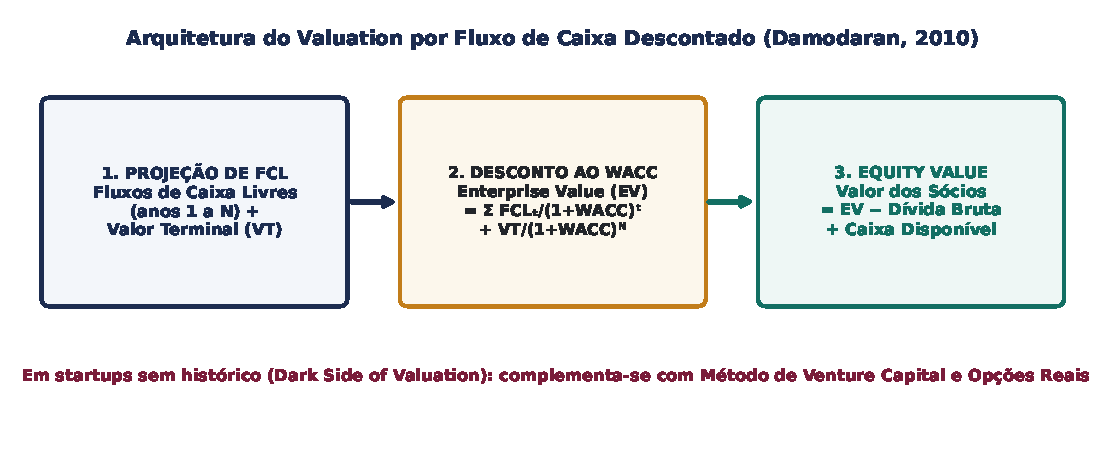
\includegraphics[width=0.94\textwidth]{figures/fig14_valuation_fcd_vc.pdf}
  \caption{Arquitetura de Valuation: Fluxo de Caixa Descontado (WACC, Gordon, EV e Equity) versus Método de Venture Capital.}
  \label{fig:14_valuation}
\end{figure}

\subsection{\textit{The Dark Side of Valuation}, Venture Capital e Opções Reais}

Quando tentamos aplicar o FCD tradicional a startups nascentes, de base tecnológica ou projetos de impacto em estágio pré-operacional, enfrentamos o que Damodaran (2010) denomina \textit{The Dark Side of Valuation}: ausência de histórico contábil, fluxos de caixa negativos nos primeiros anos, alta taxa de mortalidade e incerteza sobre o tamanho futuro do mercado. Nesses casos, dois instrumentos complementam ou substituem o FCD:

\begin{boxConceito}[Método de Venture Capital e Opções Reais]
\begin{enumerate}[leftmargin=1.4em, itemsep=3pt]
  \item \textbf{Método de Venture Capital (VC):} o fundo parte do futuro para o presente. Estima o \textbf{Valor de Saída ($EV_{\text{saída}}$)} em um horizonte $n$ (tipicamente $3$ a $7$ anos) aplicando um múltiplo de mercado (ex.: $EV/EBITDA$ ou $EV/\text{Receita}$) sobre a métrica projetada. Em seguida, desconta esse valor pela \textbf{TIR-alvo do fundo} ($r_{VC}$, alta para compensar o risco do portfólio):
  \[
    \text{Post-money} = \frac{\text{Valor de Saída}}{(1 + r_{VC})^n}, \qquad \text{Pre-money} = \text{Post-money} - \text{Aporte}, \qquad \%\text{Participação} = \frac{\text{Aporte}}{\text{Post-money}}
  \]
  \item \textbf{Opções Reais:} diferente do VPL estático (que assume decisão rígida ``agora ou nunca''), a teoria de Opções Reais incorpora o valor econômico da \textbf{flexibilidade gerencial}: o direito, mas não a obrigação, de \textbf{adiar} o investimento aguardando redução de incerteza, \textbf{expandir} a planta se a demanda superar o esperado, ou \textbf{abandonar} o projeto vendendo ativos caso o cenário seja adverso. Assim:
  \[
    VPL_{\text{expandido}} = VPL_{\text{estático}} + \text{Valor da Opção Real}
  \]
\end{enumerate}
\end{boxConceito}

\etapa{4}{Exemplos Resolvidos Passo a Passo}

\begin{boxExemplo}{14.1}{Cálculo do Custo Médio Ponderado de Capital (WACC)}
\passoEnunciado{Uma empresa de tecnologia limpa instalada em parque tecnológico regional financia suas operações com capital próprio e dívida de longo prazo junto a banco de fomento.}
\passoDados{Valor de mercado do Patrimônio Líquido ($E$) = \reais{6.000.000}; Dívida onerosa ($D$) = \reais{4.000.000}; Custo do capital próprio ($K_e$) = $16\%$ a.a.; Custo da dívida antes dos impostos ($K_d$) = $10\%$ a.a.; Alíquota efetiva de IR/CSLL ($T$) = $34\%$.}
\passoPedido{Calcular os pesos de capital ($E/(D+E)$ e $D/(D+E)$) e o $WACC$ anual da empresa.}
\passoMetodo{Cálculo da estrutura de capital total ($D+E$), aplicação do escudo fiscal na dívida $K_d(1-T)$ e média ponderada.}
\passoContas{%
\begin{align*}
  D + E &= 4.000.000 + 6.000.000 = \reais{10.000.000} \\
  \frac{E}{D + E} &= \frac{6.000.000}{10.000.000} = 0{,}60 \ (60\%), \qquad \frac{D}{D + E} = \frac{4.000.000}{10.000.000} = 0{,}40 \ (40\%) \\[4pt]
  K_d (1 - T) &= 10\% \times (1 - 0{,}34) = 10\% \times 0{,}66 = 6{,}60\% \\[4pt]
  WACC &= (0{,}60 \times 16\%) + (0{,}40 \times 6{,}60\%) \\
  &= 9{,}60\% + 2{,}64\% = 12{,}24\%\text{ a.a.}
\end{align*}
}
\passoResposta{O Custo Médio Ponderado de Capital ($WACC$) é de \textbf{12,24\% a.a.}}
\passoVerificacao{O $WACC$ ($12{,}24\%$) situa-se entre o custo líquido da dívida ($6{,}60\%$) e o custo do capital próprio ($16\%$), refletindo exatamente o peso de $60\%$ de sócios e $40\%$ de credores.}
\end{boxExemplo}

\begin{boxExemplo}{14.2}{Valuation Completo por FCD: Gordon, Enterprise Value e Equity Value}
\passoEnunciado{Um fundo de investimento avalia a aquisição de uma empresa de automação agrícola que possui projeção explícita de FCL para os próximos $3$ anos.}
\passoDados{$FCL_1 = \reais{500.000}$, $FCL_2 = \reais{600.000}$, $FCL_3 = \reais{720.000}$. $WACC = 12\%$ a.a.; taxa de crescimento perpétuo após o Ano $3$ ($g$) = $3\%$ a.a. A empresa possui Dívida Bruta de \reais{1.500.000}, Caixa de \reais{300.000} e $1.000.000$ de ações emitidas.}
\passoPedido{Calcular o Valor Presente dos FCLs explícitos, o Valor Terminal ($VT_3$), o $EV$, o $Equity\ Value$ e o valor justo por ação.}
\passoMetodo{Desconto individual de $FCL_1, FCL_2, FCL_3$ a $12\%$; aplicação da perpetuidade de Gordon em $t=3$; desconto de $VT_3$ por $(1{,}12)^3$; ajuste de dívida e caixa.}
\passoContas{%
\begin{align*}
  VP(FCL_{1..3}) &= \frac{500.000}{1{,}12} + \frac{600.000}{1{,}12^2} + \frac{720.000}{1{,}12^3} \\
  &= 446.428{,}57 + 478.316{,}33 + 512.481{,}78 = \reais{1.437.226{,}68} \\[6pt]
  VT_3 &= \frac{720.000 \times (1 + 0{,}03)}{0{,}12 - 0{,}03} = \frac{741.600}{0{,}09} = \reais{8.240.000{,}00} \\
  VP(VT_3) &= \frac{8.240.000}{1{,}12^3} = \frac{8.240.000}{1{,}404928} = \reais{5.865.069{,}24} \\[6pt]
  EV &= 1.437.226{,}68 + 5.865.069{,}24 = \reais{7.302.295{,}92} \\
  Equity &= 7.302.295{,}92 - 1.500.000 + 300.000 = \reais{6.102.295{,}92} \\
  \text{Preço justo por ação} &= \frac{6.102.295{,}92}{1.000.000} \approx \reais{6{,}10/\text{ação}}
\end{align*}
}
\passoResposta{$EV = \mathbf{\reais{7.302.295{,}92}}$; $Equity\ Value = \mathbf{\reais{6.102.295{,}92}}$; Valor por ação = \textbf{\reais{6,10}}.}
\passoVerificacao{Note que $VP(VT_3)$ representa $80{,}3\%$ do $EV$ total ($\frac{5{,}865}{7{,}302}$), fenômeno clássico em \textit{Valuation} que exige rigor na escolha de $g$ (nunca superior ao crescimento nominal de longo prazo da economia).}
\end{boxExemplo}

\begin{boxExemplo}{14.3}{Método de Venture Capital: Post-money, Pre-money e Participação}
\passoEnunciado{Uma healthtech universitária busca um aporte de \reais{2.000.000} junto a um fundo de Venture Capital para escalar sua plataforma de telemonitoramento no SUS regional.}
\passoDados{Aporte solicitado = \reais{2.000.000}; horizonte de saída do fundo ($n$) = $4$ anos; EBITDA projetado no Ano $4$ = \reais{2.500.000}; múltiplo setorial de saída ($EV/EBITDA$) = $8\times$; TIR-alvo exigida pelo fundo ($r_{VC}$) = $40\%$ a.a. (sem dívida ou caixa relevantes na saída).}
\passoPedido{Calcular o Valor de Saída, o \textit{Post-money Valuation}, o \textit{Pre-money Valuation} e o percentual de participação societária exigido pelo fundo.}
\passoMetodo{Cálculo de $\text{Saída} = EBITDA_4 \times 8$; desconto por $(1{,}40)^4$ para achar o \textit{Post-money}; subtração do aporte para o \textit{Pre-money}; divisão $\text{Aporte}/\text{Post-money}$.}
\passoContas{%
\begin{align*}
  \text{Valor de Saída (Ano 4)} &= 2.500.000 \times 8 = \reais{20.000.000{,}00} \\[4pt]
  \text{Post-money} &= \frac{20.000.000}{(1{,}40)^4} = \frac{20.000.000}{3{,}8416} = \reais{5.206.164{,}10} \\[4pt]
  \text{Pre-money} &= 5.206.164{,}10 - 2.000.000 = \reais{3.206.164{,}10} \\[4pt]
  \%\text{Participação do Fundo} &= \frac{2.000.000}{5.206.164{,}10} \times 100\% = 38{,}42\%
\end{align*}
}
\passoResposta{Saída = \textbf{\reais{20,00 mi}}; \textit{Post-money} = \textbf{\reais{5.206.164,10}}; \textit{Pre-money} = \textbf{\reais{3.206.164,10}}; Participação exigida = \textbf{38,42\%}.}
\passoVerificacao{Se os fundadores aceitarem ceder $38{,}42\%$ hoje, em $4$ anos essa fatia valerá $0{,}3842 \times 20.000.000 = \reais{7.684.000}$, entregando exatamente os $40\%$ ao ano compostos sobre os \reais{2,00 mi} investidos ($2{,}0 \times 3{,}8416 = 7{,}6832\text{ mi}$).}
\end{boxExemplo}

\begin{boxExemplo}{14.4}{Dark Side of Valuation: Múltiplo de Receita Recorrente (ARR) em Startup Inicial}
\passoEnunciado{Uma agtech SaaS (software como serviço para gestão de cooperativas) possui apenas $18$ meses de operação, margem EBITDA ainda negativa ($-\reais{300.000/\text{ano}}$) devido a gastos de P\&D, mas forte tração comercial.}
\passoDados{Receita Recorrente Anual ($ARR$) atual = \reais{1.200.000}; crescimento anual de $50\%$; empresas SaaS comparáveis no mercado brasileiro negociam a um múltiplo mediano $EV/ARR = 4{,}0\times$.}
\passoPedido{Explicar por que o FCD tradicional com base no lucro atual falha e estimar o $EV$ referencial pelo múltiplo de $ARR$.}
\passoMetodo{Aplicação de avaliação relativa por múltiplo de receita ($EV = ARR \times \text{Múltiplo}$), típica de startups em estágio de crescimento com margem negativa.}
\passoContas{%
\[
  EV_{\text{ARR}} = 1.200.000 \times 4{,}0 = \reais{4.800.000{,}00}
\]
}
\passoResposta{$EV$ referencial de \textbf{\reais{4.800.000,00}}.}
\passoVerificacao{Um múltiplo de $EBITDA$ seria impossível (geraria valor negativo). O múltiplo de $ARR$ contorna o \textit{Dark Side of Valuation} no curto prazo, desde que a startup apresente economia unitária saudável ($LTV > 3 \times CAC$) que garanta lucratividade futura.}
\end{boxExemplo}

\begin{boxExemplo}{14.5}{Opções Reais: Valor da Flexibilidade de Abandono em Biorrefinaria}
\passoEnunciado{Um projeto piloto de biorrefinaria de resíduos agroindustriais exige investimento inicial $I_0 = \reais{1.000.000}$. No Ano $1$, o mercado se define com igual probabilidade ($50\%$) entre um cenário favorável (Valor Presente dos fluxos futuros em $t=1$ igual a \reais{1.600.000}) e um cenário adverso (Valor Presente igual a \reais{600.000}). A $TMA$ é de $10\%$ a.a.}
\passoDados{$I_0 = \reais{1.000.000}$; $p_{\text{bom}} = 0{,}50$ ($V_1 = 1.600.000$); $p_{\text{ruim}} = 0{,}50$ ($V_1 = 600.000$); $TMA = 10\%$. Entretanto, o contrato permite \textbf{abandonar} o projeto no Ano $1$ e liquidar os equipamentos modulares por \reais{800.000}.}
\passoPedido{Calcular o $VPL_{\text{estático}}$ (sem opção de abandono), o $VPL_{\text{expandido}}$ (com opção de abandono) e o Valor da Opção Real ($VOR$).}
\passoMetodo{Cálculo do valor esperado em $t=1$ sem flexibilidade e com substituição do payoff adverso pelo valor de liquidação ($\max(600.000;\, 800.000) = 800.000$), descontado a $10\%$.}
\passoContas{%
\begin{align*}
  VPL_{\text{estático}} &= \frac{(0{,}50 \times 1.600.000) + (0{,}50 \times 600.000)}{1{,}10} - 1.000.000 \\
  &= \frac{800.000 + 300.000}{1{,}10} - 1.000.000 = \frac{1.100.000}{1{,}10} - 1.000.000 = \reais{0{,}00} \\[6pt]
  VPL_{\text{expandido}} &= \frac{(0{,}50 \times 1.600.000) + (0{,}50 \times \max(600.000;\, 800.000))}{1{,}10} - 1.000.000 \\
  &= \frac{800.000 + 400.000}{1{,}10} - 1.000.000 = \frac{1.200.000}{1{,}10} - 1.000.000 \\
  &= 1.090.909{,}09 - 1.000.000 = +\reais{90.909{,}09} \\[6pt]
  VOR &= VPL_{\text{expandido}} - VPL_{\text{estático}} = 90.909{,}09 - 0 = \reais{90.909{,}09}
\end{align*}
}
\passoResposta{$VPL_{\text{estático}} = \mathbf{\reais{0{,}00}}$; $VPL_{\text{expandido}} = \mathbf{+\reais{90.909{,}09}}$; Valor da Opção Real de Abandono = \textbf{\reais{90.909,09}}.}
\passoVerificacao{Pela análise estática ($VPL = 0$), o projeto seria indiferente e provavelmente descartado. Ao incorporar equipamentos modulares com mercado secundário (flexibilidade de abandono), o risco de perda extrema é limitado e o projeto passa a criar \reais{90.909,09} de valor líquido.}
\end{boxExemplo}

\etapa{5}{Armadilhas Conceituais e Erros Mais Comuns}

\begin{boxErro}[Erro 1: Assumir taxa de crescimento perpétuo $g \ge WACC$ na fórmula de Gordon]
Se $g \ge WACC$, o denominador $(WACC - g)$ torna-se zero ou negativo, produzindo valor infinito ou negativo absurdo. Além disso, nenhuma empresa pode crescer perpetuamente acima do PIB nominal da economia sem se tornar maior que o próprio mercado.
\end{boxErro}

\begin{boxErro}[Erro 2: Esquecer o benefício fiscal da dívida $(1 - T)$ no WACC]
Os juros pagos sobre empréstimos são dedutíveis da base de cálculo do IR/CSLL no lucro real. Usar $K_d$ bruto em vez de $K_d(1-T)$ superestima o WACC e subestima o $Enterprise\ Value$.
\end{boxErro}

\begin{boxErro}[Erro 3: Confundir Enterprise Value ($EV$) com Equity Value ($Equity$)]
Ao vender $100\%$ das quotas ou negociar uma rodada de investimento, o valor que pertence aos acionistas é o \textbf{Equity Value} ($EV - \text{Dívida Bruta} + \text{Caixa}$), não o $EV$. Ignorar a dívida na negociação faz o comprador assumir passivos sem ajuste de preço.
\end{boxErro}

\begin{boxErro}[Erro 4: Usar $FCL_n$ em vez de $FCL_{n+1}$ no numerador de Gordon]
Na perpetuidade de Gordon aplicada ao final do ano $n$, o numerador exige o fluxo do primeiro ano da perpetuidade: $FCL_{n+1} = FCL_n (1+g)$. Esquecer o fator $(1+g)$ subestima o Valor Terminal.
\end{boxErro}

\etapa{6}{Lista de Exercícios de Fixação (15 Questões)}

\begin{enumerate}[leftmargin=1.6em, itemsep=5pt]
  \item Diferencie \textbf{preço} de \textbf{valor intrínseco} segundo Damodaran (2010), explicando por que uma startup pode ser negociada a um preço acima ou abaixo de seu valor fundamental. \espacoResolucao[1.5cm]
  \item Calcule o custo do capital próprio ($K_e$) pelo modelo CAPM sabendo que a taxa livre de risco ($R_f$) é $10\%$ a.a., o beta ($\beta$) setorial é $1{,}2$ e o prêmio de risco de mercado ($R_m - R_f$) é $5\%$ a.a. \espacoResolucao[1.5cm]
  \item Uma empresa tem estrutura de capital composta por $70\%$ de capital próprio ($K_e = 15\%$ a.a.) e $30\%$ de dívida ($K_d = 10\%$ a.a.), com alíquota de IR/CSLL $T = 34\%$. Calcule o $WACC$. \espacoResolucao[1.6cm]
  \item Uma firma gera $FCL_n = \reais{400.000}$ no último ano do horizonte explícito, com crescimento perpétuo $g = 4\%$ a.a. e $WACC = 12\%$ a.a. Calcule o Valor Terminal ($VT_n$) pela perpetuidade de Gordon. \espacoResolucao[1.6cm]
  \item Sabendo que o \textit{Enterprise Value} ($EV$) de uma empresa é \reais{8.500.000}, sua Dívida Bruta é de \reais{2.200.000} e seu Caixa disponível é de \reais{700.000}, calcule o \textit{Equity Value}. \espacoResolucao[1.5cm]
  \item Calcule o $EV$ completo de uma startup madura com $FCL_1 = \reais{300.000}$, $FCL_2 = \reais{360.000}$, $WACC = 10\%$ a.a. e crescimento perpétuo $g = 2\%$ a.a. após o Ano $2$. \espacoResolucao[2.0cm]
  \item Pelo Método de Venture Capital, um fundo projeta que uma edtech valerá \reais{12.500.000} na saída no Ano $3$ e exige uma TIR-alvo de $50\%$ a.a. Se o fundo aportar \reais{1.000.000} hoje, calcule o \textit{Post-money}, o \textit{Pre-money} e a participação societária (\%) exigida. \espacoResolucao[1.9cm]
  \item Um empreendedor detém $100\%$ de sua startup. Na rodada Seed, vende $20\%$ da empresa para um investidor anjo. Dois anos depois, na Série A, um fundo entra adquirindo $25\%$ da empresa (diluição proporcional). Qual será a participação final do fundador após a Série A? \espacoResolucao[1.6cm]
  \item Um projeto possui $VPL_{\text{estático}} = -\reais{100.000}$ ($VP = \reais{900.000}$ e $I_0 = \reais{1.000.000}$). Entretanto, no Ano $1$, com probabilidade de $40\%$, a empresa pode exercer uma \textbf{opção real de expansão}: investir \reais{400.000} adicionais para gerar um valor presente adicional de \reais{950.000} em $t=1$. À $TMA = 10\%$ a.a., qual é o $VPL_{\text{expandido}}$? \espacoResolucao[1.9cm]
  \item Por que o modelo FCD apresenta limitações severas (\textit{The Dark Side of Valuation}) quando aplicado a startups pré-operacionais ou projetos de P\&D profundo? \espacoResolucao[1.5cm]
  \item Explique por que o Valor Terminal costuma responder por $60\%$ a $85\%$ do $EV$ total em empresas em crescimento e qual o risco de inflar a taxa $g$ na avaliação. \espacoResolucao[1.5cm]
  \item Em negócios de impacto territorial (como cooperativas tecnológicas ou bioeconomia), como o retorno socioambiental não precificado no FCL dialoga com o valor econômico estimado? \espacoResolucao[1.5cm]
  \item Qual é a diferença conceitual entre descontar o $FCL$ pelo $WACC$ (para achar o $EV$) e descontar o Valor de Saída pela TIR-alvo no Método de Venture Capital? \espacoResolucao[1.5cm]
  \item Cite e exemplifique os três tipos principais de Opções Reais em projetos tecnológicos: opção de adiar, opção de expandir e opção de abandonar. \espacoResolucao[1.5cm]
  \item Se uma empresa possui mais Caixa do que Dívida Bruta (Dívida Líquida negativa), o seu \textit{Equity Value} será maior ou menor que o seu \textit{Enterprise Value}? Justifique pela equação contábil. \espacoResolucao[1.5cm]
\end{enumerate}

\etapa{7}{Desafios Autorais e Aplicação Territorial (Preparação AV3)}

\begin{enumerate}[leftmargin=1.6em, itemsep=5pt]
  \item \textbf{Valuation do Projeto da AV3:} Estime o $EV$ e o $Equity\ Value$ do empreendimento do seu grupo utilizando o FCD em $3$ a $5$ anos com perpetuidade conservadora ($g \le 3\%$ a.a.), explicitando a composição do $WACC$. \espacoResolucao[2.0cm]
  \item \textbf{Simulação de Rodada de Investimento:} Suponha que seu grupo precise captar o CAPEX inicial via investidor-anjo ou fundo de impacto com TIR-alvo de $30\%$ a.a. em $4$ anos. Calcule qual percentual societário seria cedido pelo Método de Venture Capital e avalie se a diluição é aceitável para os fundadores. \espacoResolucao[1.9cm]
  \item \textbf{Flexibilidade Territorial:} Identifique uma Opção Real concreta no projeto da AV3 (ex.: implantar em módulos escaláveis conforme adesão da cooperativa ou manter opção de uso alternativo do galpão) e explique como ela reduz o risco de perda máxima. \espacoResolucao[1.6cm]
\end{enumerate}

\begin{boxDica}[Contraponto Crítico e Prática Territorial (AV2 e AV3)]
Ao apresentar um \textit{Valuation} para investidores ou bancos de fomento, evite ``planilhas mágicas'' em que o Valor Terminal justifica sozinho um negócio deficitário nos primeiros cinco anos. Mostre em quanto tempo o negócio atinge o equilíbrio operacional (Cap. 12), qual é o VPL dos fluxos explícitos (Cap. 13) e qual é o múltiplo implícito na saída (Cap. 14).
\end{boxDica}

\clearpage
\etapa{8}{Gabarito Integralmente Comentado (Exercícios 1 a 15 + Desafios 1 a 3)}

\begin{boxGabarito}[Resolução Passo a Passo — Exercícios de Fixação (1 a 15)]
\begin{enumerate}[leftmargin=1.5em, itemsep=4pt]
  \item \textbf{Preço vs. Valor:} Valor intrínseco reflete a geração futura de caixa descontada pelo risco; preço é o resultado da negociação de mercado em dado momento, podendo desviar-se do valor por escassez de liquidez, euforia ou assimetria de informação.
  \item \textbf{CAPM:} $K_e = 10\% + 1{,}2 \times 5\% = 10\% + 6\% = \mathbf{16{,}00\%\text{ a.a.}}$.
  \item \textbf{WACC:} $WACC = (0{,}70 \times 15\%) + (0{,}30 \times 10\% \times (1 - 0{,}34)) = 10{,}50\% + 1{,}98\% = \mathbf{12{,}48\%\text{ a.a.}}$.
  \item \textbf{Gordon:} $FCL_{n+1} = 400.000 \times 1{,}04 = \reais{416.000}$. $VT_n = 416.000 / (0{,}12 - 0{,}04) = 416.000 / 0{,}08 = \mathbf{\reais{5.200.000}}$.
  \item \textbf{EV para Equity:} $Equity = 8.500.000 - 2.200.000 + 700.000 = \mathbf{\reais{7.000.000}}$.
  \item \textbf{FCD completo:}
  $VT_2 = \frac{360.000 \times 1{,}02}{0{,}10 - 0{,}02} = \frac{367.200}{0{,}08} = \reais{4.590.000}$. \\
  $EV = \frac{300.000}{1{,}10} + \frac{360.000 + 4.590.000}{1{,}10^2} = 272.727{,}27 + \frac{4.950.000}{1{,}21} = 272.727{,}27 + 4.090.909{,}09 = \mathbf{\reais{4.363.636{,}36}}$.
  \item \textbf{Venture Capital:}
  $\text{Post-money} = \frac{12.500.000}{1{,}50^3} = \frac{12.500.000}{3{,}375} = \mathbf{\reais{3.703.703{,}70}}$. \\
  $\text{Pre-money} = 3.703.703{,}70 - 1.000.000 = \mathbf{\reais{2.703.703{,}70}}$. \\
  $\%\text{Participação} = \frac{1.000.000}{3.703.703{,}70} \times 100\% = \mathbf{27{,}00\%}$.
  \item \textbf{Diluição:} Após Seed, fundador mantém $80\%$. Na Série A, novos investidores ficam com $25\%$, restando $75\%$ para os acionistas anteriores: $0{,}80 \times 0{,}75 = \mathbf{60{,}00\%}$ para o fundador.
  \item \textbf{Opção de Expansão:} No Ano $1$, o ganho líquido da expansão é $950.000 - 400.000 = \reais{550.000}$ (positivo, logo a opção é exercida se o cenário ocorrer). $VP(\text{Opção}) = \frac{0{,}40 \times 550.000}{1{,}10} = \frac{220.000}{1{,}10} = \reais{200.000}$. Assim, $VPL_{\text{expandido}} = -100.000 + 200.000 = \mathbf{+\reais{100.000}}$.
  \item \textbf{Dark Side:} Startups jovens não têm histórico de receita estável, operam com margens negativas, dependem de rodadas futuras incertas e têm alta taxa de fracasso, tornando o $FCL$ de curto prazo negativo e o $VT$ extremamente sensível a premissas especulativas.
  \item \textbf{Peso do VT:} Em empresas em expansão, o caixa se concentra no longo prazo após a maturação do CAPEX. Inflar $g$ reduz $(WACC - g)$ no denominador, multiplicando artificialmente o $VT$ e distorcendo o $EV$.
  \item \textbf{Impacto territorial:} O $Valuation$ financeiro mede o valor capturável em moeda pelo empreendimento; externalidades positivas (emprego local, conservação de solo/água, segurança alimentar) devem ser reportadas paralelamente por métricas de impacto (Cap. 5) para atrair capital paciente ou subvenção.
  \item \textbf{WACC vs. TIR-alvo VC:} O $WACC$ reflete o custo ponderado de capital de uma empresa em operação contínua com risco estabilizado. A TIR-alvo de VC ($30\%$ a $60\%$) incorpora o risco de mortalidade e iliquidez de startups, servindo como taxa de desconto ajustada ao portfólio do fundo.
  \item \textbf{Tipos de Opções Reais:} \textit{Adiar}: esperar definição regulatória ou preço de commodity antes de construir; \textit{Expandir}: instalar planta modular com capacidade de dobrar linha de produção se a demanda validar; \textit{Abandonar}: vender ativos ou sublocar estrutura caso o mercado fracasse.
  \item \textbf{Caixa > Dívida:} Pela equação $Equity = EV - \text{Dívida Bruta} + \text{Caixa}$, se $\text{Caixa} > \text{Dívida Bruta}$, soma-se um valor líquido positivo ao $EV$, logo o \textbf{Equity Value será maior que o Enterprise Value}.
\end{enumerate}
\end{boxGabarito}

\begin{boxGabarito}[Diretrizes de Resposta — Desafios Autorais (1 a 3)]
\begin{enumerate}[leftmargin=1.5em, itemsep=3pt]
  \item \textbf{Desafio 1:} Deve apresentar $WACC$ coerente com a estrutura de financiamento do projeto (ex.: parcela subsidiada FNE/BNDES como $D$ e capital dos sócios como $E$), calcular $VT_n$ com $g < WACC$ e realizar a passagem $EV \to Equity$.
  \item \textbf{Desafio 2:} Deve projetar uma métrica de saída realista ($EBITDA_4 \times \text{múltiplo}$), descontar por $(1{,}30)^4 = 2{,}8561$ para obter o \textit{Post-money} e discutir o equilíbrio entre capital captado e governança dos fundadores.
  \item \textbf{Desafio 3:} Deve demonstrar como a modularização de investimentos reduz o comprometimento irreversível de capital no Ano $0$, convertendo risco de perda fixa em opção estratégica de baixo custo.
\end{enumerate}
\end{boxGabarito}

\begin{boxResumo}
\begin{itemize}[leftmargin=1.4em, itemsep=2pt]
  \item \textit{Valuation} estima o \textbf{valor intrínseco} pelos fundamentos, distinto do \textbf{preço} negociado.
  \item No \textbf{FCD} (Damodaran, 2010), desconta-se o $FCL$ e o Valor Terminal de Gordon ($VT_n = \frac{FCL_{n+1}}{WACC - g}$) pelo $WACC$ para obter o $EV$, ajustando-se Dívida e Caixa para chegar ao $Equity\ Value$.
  \item Em startups sem histórico (\textit{Dark Side}), o \textbf{Método de Venture Capital} parte do valor de saída descontado pela TIR-alvo do fundo para definir \textit{Post-money}, \textit{Pre-money} e participação.
  \item \textbf{Opções Reais} quantificam o valor da flexibilidade gerencial de adiar, expandir ou abandonar projetos.
\end{itemize}
\end{boxResumo}

\begin{boxTeste}
\begin{enumerate}[leftmargin=1.5em, itemsep=4pt]
  \item Calcule o $WACC$ de uma empresa com $80\%$ de capital próprio ($K_e = 15\%$), $20\%$ de dívida ($K_d = 10\%$) e alíquota $T = 30\%$.
  \item Se $EV = \reais{5.000.000}$, Dívida Bruta = \reais{1.200.000} e Caixa = \reais{400.000}, qual é o \textit{Equity Value}?
  \item (\V/\F) Na fórmula de Gordon, a taxa de crescimento perpétuo $g$ deve ser estritamente menor que o $WACC$.
  \item (\V/\F) Na análise de Opções Reais, a flexibilidade gerencial de abandonar um projeto deficitário reduz seu valor em relação ao $VPL$ estático.
\end{enumerate}
\vspace{4pt}
\noindent\textbf{Gabarito do Checkpoint:} \textbf{1.} $WACC = 0{,}80(15\%) + 0{,}20(10\%)(1 - 0{,}30) = 12{,}00\% + 1{,}40\% = \mathbf{13{,}40\%\text{ a.a.}}$. \quad \textbf{2.} $Equity = 5.000.000 - 1.200.000 + 400.000 = \mathbf{\reais{4.200.000}}$. \quad \textbf{3.} \V. \quad \textbf{4.} \F\ (aumenta ou preserva valor ao limitar perdas nos cenários adversos).
\end{boxTeste}

\clearpage
\phantomsection
\addcontentsline{toc}{chapter}{Simulado III — Preparatório AV2 (20\%) e Engenharia Financeira}
\chapter*{Simulado III — Estudo Dirigido Quantitativo (AV2 — 20\%)}
\markboth{SIMULADO III — PREPARATÓRIO AV2}{SIMULADO III — PREPARATÓRIO AV2}

\noindent\tagAV{SIMULADO AV2 (20\%)}\ \tagQuant\ \tagTerritorio
\vspace{6pt}

\begin{tcolorbox}[colback=bgSoft, colframe=etIndigo, boxrule=0.8pt, arc=3pt, title={\bfseries INSTRUÇÕES DE APLICAÇÃO E RESOLUÇÃO}, coltitle=white, colbacktitle=etIndigo]
Este simulado reproduz o padrão quantitativo e analítico da \textbf{AV2 (20\%)} e consolida a engenharia financeira exigida na defesa da \textbf{AV3}. Resolva as \textbf{8 questões objetivas} (múltipla escolha A--E) e as \textbf{2 questões dissertativas} sem consultar o gabarito antes de concluir todas as contas. Ao final, confira cada passo numérico no Gabarito Integralmente Comentado e preencha a Tabela de Diagnóstico.
\end{tcolorbox}

\section*{Parte I — Questões Objetivas de Cálculo Integral (8 Questões)}

\begin{enumerate}[leftmargin=1.6em, itemsep=8pt]

  \item \textbf{(Matriz Locacional Ponderada — Cap. 12)} Uma agroindústria de bioembalagens avalia três municípios ($A$, $B$ e $C$) segundo três critérios ponderados: Logística ($w_1 = 0{,}40$), Infraestrutura Energética/Hídrica ($w_2 = 0{,}35$) e Proximidade a Centros de P\&D ($w_3 = 0{,}25$). As notas atribuídas de $0$ a $10$ foram:
  \begin{center}
  \small
  \begin{tabular}{@{}lccc@{}}
    \toprule
    \textbf{Critério (Peso)} & \textbf{Município A} & \textbf{Município B} & \textbf{Município C} \\
    \midrule
    Logística ($0{,}40$) & 8 & 9 & 7 \\
    Energia e Água ($0{,}35$) & 8 & 6 & 8 \\
    Centros de P\&D ($0{,}25$) & 6 & 8 & 8 \\
    \bottomrule
  \end{tabular}
  \end{center}
  Com base na Matriz Locacional Ponderada, o município vencedor e sua pontuação final são:
  \begin{alternativas}
    \item Município A, com 7,50 pontos.
    \item Município C, com 7,60 pontos.
    \item Município B, com 7,70 pontos.
    \item Município B, com 7,85 pontos.
    \item Empate entre B e C, com 7,65 pontos.
  \end{alternativas}

  \item \textbf{(Capital de Giro e Ponto de Equilíbrio — Cap. 12)} Uma startup de sensores ambientais apresenta os seguintes prazos médios operacionais: $PME = 25$ dias, $PMR = 35$ dias e $PMP = 20$ dias, com OPEX desembolsável anual de \reais{900.000} (ano comercial de $360$ dias). Em sua estrutura de custos, os custos fixos anuais somam \reais{144.000}, o preço unitário de venda é \reais{150,00} e o custo variável unitário é \reais{90,00}. Assinale a alternativa que apresenta corretamente a Necessidade Líquida de Capital de Giro ($NLCG$) e o Ponto de Equilíbrio Contábil em unidades ($PE_{\text{unid}}$):
  \begin{alternativas}
    \item $NLCG = \reais{80.000}$ e $PE_{\text{unid}} = 1.600$ unidades.
    \item $NLCG = \reais{100.000}$ e $PE_{\text{unid}} = 2.400$ unidades.
    \item $NLCG = \reais{100.000}$ e $PE_{\text{unid}} = 1.600$ unidades.
    \item $NLCG = \reais{150.000}$ e $PE_{\text{unid}} = 2.400$ unidades.
    \item $NLCG = \reais{200.000}$ e $PE_{\text{unid}} = 2.880$ unidades.
  \end{alternativas}

  \item \textbf{(Valor Presente Líquido — Cap. 13)} Um projeto de irrigação inteligente exige investimento inicial de \reais{120.000} em $t=0$ e gera fluxos de caixa livres de \reais{55.000} no Ano $1$, \reais{60.500} no Ano $2$ e \reais{66.550} no Ano $3$. Considerando uma $TMA = 10\%$ a.a., o Valor Presente Líquido ($VPL$) do projeto é:
  \begin{alternativas}
    \item $+\reais{15.000,00}$
    \item $+\reais{25.000,00}$
    \item $+\reais{30.000,00}$
    \item $+\reais{45.000,00}$
    \item $+\reais{62.050,00}$
  \end{alternativas}

  \item \textbf{(Payback Descontado — Cap. 13)} Uma cooperativa investe \reais{100.000} em $t=0$ para modernizar sua unidade de beneficiamento, projetando fluxos de caixa livres de \reais{44.000} (Ano $1$), \reais{48.400} (Ano $2$) e \reais{53.240} (Ano $3$). Adotando $TMA = 10\%$ a.a., o Payback Descontado ($PBD$) do projeto é de:
  \begin{alternativas}
    \item $2{,}00$ anos.
    \item $2{,}15$ anos.
    \item $2{,}25$ anos.
    \item $2{,}50$ anos.
    \item $2{,}75$ anos.
  \end{alternativas}

  \item \textbf{(VAUE para Vidas Úteis Diferentes — Cap. 13)} Uma empresa deve escolher entre dois equipamentos mutuamente excludentes e renováveis à $TMA = 10\%$ a.a.: o Equipamento Alfa tem vida útil de $2$ anos e $VPL_{\text{Alfa}} = \reais{21.000,00}$; o Equipamento Beta tem vida útil de $3$ anos e $VPL_{\text{Beta}} = \reais{24.868,52}$. Calcule o Valor Anual Uniforme Equivalente ($VAUE$) de cada alternativa e assinale a decisão correta:
  \begin{alternativas}
    \item $VAUE_{\text{Alfa}} = \reais{10.500,00/\text{ano}}$ e $VAUE_{\text{Beta}} = \reais{8.289,51/\text{ano}}$; escolher Alfa.
    \item $VAUE_{\text{Alfa}} = \reais{12.100,00/\text{ano}}$ e $VAUE_{\text{Beta}} = \reais{10.000,00/\text{ano}}$; escolher Alfa.
    \item $VAUE_{\text{Alfa}} = \reais{12.100,00/\text{ano}}$ e $VAUE_{\text{Beta}} = \reais{12.434,26/\text{ano}}$; escolher Beta.
    \item $VAUE_{\text{Alfa}} = \reais{11.550,00/\text{ano}}$ e $VAUE_{\text{Beta}} = \reais{10.000,00/\text{ano}}$; escolher Alfa.
    \item Como $VPL_{\text{Beta}} > VPL_{\text{Alfa}}$, deve-se escolher Beta independentemente da vida útil.
  \end{alternativas}

  \item \textbf{(WACC — Cap. 14)} Uma empresa de base tecnológica possui valor de mercado do capital próprio $E = \reais{6.000.000}$ e dívida onerosa $D = \reais{4.000.000}$. O custo do capital próprio é $K_e = 15\%$ a.a., o custo bruto da dívida é $K_d = 10\%$ a.a. e a alíquota efetiva de IR/CSLL é $T = 34\%$. O Custo Médio Ponderado de Capital ($WACC$) dessa empresa é:
  \begin{alternativas}
    \item $10{,}64\%$ a.a.
    \item $11{,}64\%$ a.a.
    \item $12{,}00\%$ a.a.
    \item $13{,}00\%$ a.a.
    \item $13{,}40\%$ a.a.
  \end{alternativas}

  \item \textbf{(FCD, Gordon, EV e Equity Value — Cap. 14)} Na avaliação por Fluxo de Caixa Descontado de uma empresa com $WACC = 10\%$ a.a., projetaram-se $FCL_1 = \reais{220.000}$ e $FCL_2 = \reais{242.000}$, além de crescimento perpétuo $g = 2\%$ a.a. após o Ano $2$. Sabe-se que a empresa possui Dívida Bruta de \reais{1.000.000} e Caixa de \reais{300.000}. O \textit{Enterprise Value} ($EV$) e o \textit{Equity Value} ($Equity$) são, respectivamente:
  \begin{alternativas}
    \item $EV = \reais{2.550.000}$ e $Equity = \reais{1.850.000}$.
    \item $EV = \reais{2.950.000}$ e $Equity = \reais{2.250.000}$.
    \item $EV = \reais{2.950.000}$ e $Equity = \reais{1.950.000}$.
    \item $EV = \reais{3.085.500}$ e $Equity = \reais{2.385.500}$.
    \item $EV = \reais{3.485.500}$ e $Equity = \reais{2.785.500}$.
  \end{alternativas}

  \item \textbf{(Método de Venture Capital — Cap. 14)} Uma startup de biotecnologia negocia um aporte de \reais{2.000.000} com um fundo de Venture Capital que exige TIR-alvo de $50\%$ a.a. em um horizonte de saída de $3$ anos. O valor de saída estimado da empresa no Ano $3$ (via múltiplo setorial de $EV/EBITDA$) é de \reais{27.000.000}. Pelo Método de Venture Capital, o \textit{Post-money Valuation}, o \textit{Pre-money Valuation} e o percentual de participação societária exigido pelo fundo são, respectivamente:
  \begin{alternativas}
    \item \reais{8.000.000}; \reais{6.000.000}; $25{,}00\%$.
    \item \reais{9.000.000}; \reais{7.000.000}; $22{,}22\%$.
    \item \reais{6.000.000}; \reais{4.000.000}; $33{,}33\%$.
    \item \reais{10.000.000}; \reais{8.000.000}; $20{,}00\%$.
    \item \reais{8.000.000}; \reais{8.000.000}; $25{,}00\%$.
  \end{alternativas}

\end{enumerate}

\section*{Parte II — Questões Dissertativas / Estudo Dirigido (2 Questões)}

\begin{enumerate}[leftmargin=1.6em, itemsep=8pt]
  \item \textbf{(Integração Locacional, Ponto de Equilíbrio e Análise de Investimentos — Caps. 12 e 13)} Uma cooperativa regional analisa implantar uma planta de processamento de polpa e biomassa de frutas no interior da Bahia. Explique tecnicamente: (a) como o Índice Material de Weber ($IM$) orienta a escolha entre localizar a planta junto à zona rural produtora ou na capital consumidora; (b) por que a análise do Ponto de Equilíbrio Contábil ($PE$) é necessária para gestão operacional, mas insuficiente para aprovar o investimento; e (c) quais dois problemas metodológicos da TIR justificam o uso conjunto do $VPL$ e da $MTIR$. \espacoResolucao[2.6cm]

  \item \textbf{(Valuation de Startups Tecnológicas e Projetos de Impacto — Cap. 14)} Uma agtech universitária ainda pré-lucrativa desenvolve sensores de baixo custo para agricultura familiar no Semiárido. Explique: (a) por que o Fluxo de Caixa Descontado tradicional sofre com o \textit{Dark Side of Valuation} nesse estágio; (b) como o Método de Venture Capital contorna essa limitação na definição de participação societária; e (c) como o conceito de Opções Reais (por exemplo, implantação modular escalável) agrega valor não capturado pelo $VPL$ estático. \espacoResolucao[2.6cm]
\end{enumerate}

\clearpage
\section*{Gabarito Integralmente Comentado — Simulado III}

\begin{boxGabarito}[Resolução Passo a Passo das Questões Objetivas (1 a 8)]
\begin{enumerate}[leftmargin=1.5em, itemsep=5pt]
  \item \textbf{Resposta: (C) Município B, com 7,70 pontos.} \\
  $Nota_A = (0{,}40 \times 8) + (0{,}35 \times 8) + (0{,}25 \times 6) = 3{,}20 + 2{,}80 + 1{,}50 = 7{,}50$. \\
  $Nota_B = (0{,}40 \times 9) + (0{,}35 \times 6) + (0{,}25 \times 8) = 3{,}60 + 2{,}10 + 2{,}00 = \mathbf{7{,}70}$. \\
  $Nota_C = (0{,}40 \times 7) + (0{,}35 \times 8) + (0{,}25 \times 8) = 2{,}80 + 2{,}80 + 2{,}00 = 7{,}60$.

  \item \textbf{Resposta: (B) $NLCG = \reais{100.000}$ e $PE_{\text{unid}} = 2.400$ unidades.} \\
  Ciclo Financeiro: $CF_{ciclo} = 25 + 35 - 20 = 40\text{ dias}$. \\
  Desembolso diário $= 900.000 / 360 = \reais{2.500/\text{dia}}$. \\
  $NLCG = 40 \times 2.500 = \mathbf{\reais{100.000}}$. \\
  Margem de Contribuição unitária: $MC_u = 150 - 90 = \reais{60{,}00}$. \\
  $PE_{\text{unid}} = 144.000 / 60 = \mathbf{2.400\text{ unidades}}$.

  \item \textbf{Resposta: (C) $+\reais{30.000,00}$.} \\
  $VP_1 = 55.000 / 1{,}10 = \reais{50.000{,}00}$. \\
  $VP_2 = 60.500 / 1{,}10^2 = 60.500 / 1{,}21 = \reais{50.000{,}00}$. \\
  $VP_3 = 66.550 / 1{,}10^3 = 66.550 / 1{,}331 = \reais{50.000{,}00}$. \\
  $VPL = -120.000 + 50.000 + 50.000 + 50.000 = \mathbf{+\reais{30.000{,}00}}$.

  \item \textbf{Resposta: (D) $2{,}50$ anos.} \\
  $VP_1 = 44.000 / 1{,}10 = \reais{40.000}$ $\Rightarrow$ Saldo descontado $= -100.000 + 40.000 = -\reais{60.000}$. \\
  $VP_2 = 48.400 / 1{,}21 = \reais{40.000}$ $\Rightarrow$ Saldo descontado $= -60.000 + 40.000 = -\reais{20.000}$. \\
  $VP_3 = 53.240 / 1{,}331 = \reais{40.000}$. \\
  $PBD = 2 + \frac{20.000}{40.000} = \mathbf{2{,}50\text{ anos}}$.

  \item \textbf{Resposta: (B) $VAUE_{\text{Alfa}} = \reais{12.100,00/\text{ano}}$ e $VAUE_{\text{Beta}} = \reais{10.000,00/\text{ano}}$; escolher Alfa.} \\
  $FRC(10\%, 2) = \frac{0{,}10 \times 1{,}21}{1{,}21 - 1} = \frac{0{,}121}{0{,}21} = 0{,}57619048 \Rightarrow VAUE_{\text{Alfa}} = 21.000 \times 0{,}57619048 = \mathbf{\reais{12.100{,}00/\text{ano}}}$. \\
  $FRC(10\%, 3) = \frac{0{,}10 \times 1{,}331}{1{,}331 - 1} = \frac{0{,}1331}{0{,}331} = 0{,}40211480 \Rightarrow VAUE_{\text{Beta}} = 24.868{,}52 \times 0{,}40211480 = \mathbf{\reais{10.000{,}00/\text{ano}}}$. \\
  Como $VAUE_{\text{Alfa}} > VAUE_{\text{Beta}}$, escolhe-se \textbf{Alfa}.

  \item \textbf{Resposta: (B) $11{,}64\%$ a.a.} \\
  $D + E = 4.000.000 + 6.000.000 = \reais{10.000.000}$ ($w_E = 0{,}60$, $w_D = 0{,}40$). \\
  $WACC = (0{,}60 \times 15\%) + (0{,}40 \times 10\% \times (1 - 0{,}34)) = 9{,}00\% + 2{,}64\% = \mathbf{11{,}64\%\text{ a.a.}}$.

  \item \textbf{Resposta: (B) $EV = \reais{2.950.000}$ e $Equity = \reais{2.250.000}$.} \\
  $VP(FCL_1) = 220.000 / 1{,}10 = \reais{200.000}$. \\
  $VP(FCL_2) = 242.000 / 1{,}21 = \reais{200.000}$. \\
  $VT_2 = \frac{242.000 \times 1{,}02}{0{,}10 - 0{,}02} = \frac{246.840}{0{,}08} = \reais{3.085.500}$. \\
  $VP(VT_2) = 3.085.500 / 1{,}21 = \mathbf{\reais{2.550.000}}$. \\
  $EV = 200.000 + 200.000 + 2.550.000 = \mathbf{\reais{2.950.000}}$. \\
  $Equity = 2.950.000 - 1.000.000 + 300.000 = \mathbf{\reais{2.250.000}}$.

  \item \textbf{Resposta: (A) \reais{8.000.000}; \reais{6.000.000}; $25{,}00\%$.} \\
  $\text{Post-money} = \frac{27.000.000}{(1{,}50)^3} = \frac{27.000.000}{3{,}375} = \mathbf{\reais{8.000.000}}$. \\
  $\text{Pre-money} = 8.000.000 - 2.000.000 = \mathbf{\reais{6.000.000}}$. \\
  $\%\text{Participação} = \frac{2.000.000}{8.000.000} \times 100\% = \mathbf{25{,}00\%}$.
\end{enumerate}
\end{boxGabarito}

\begin{boxGabarito}[Espelho de Correção — Questões Dissertativas (1 e 2)]
\textbf{Questão Dissertativa 1 (10 pontos):}
\begin{itemize}[leftmargin=1.4em, itemsep=2pt]
  \item \textbf{(a) Índice Material de Weber (3,5 pts):} Explicar que $IM = \text{Peso MP}/\text{Peso PA} > 1$ indica grande perda de massa (casca, água) no beneficiamento de frutas, tornando o frete da matéria-prima bruta mais caro e orientando a planta para a zona produtora rural.
  \item \textbf{(b) Limite do Ponto de Equilíbrio (3,0 pts):} Apontar que o $PE$ indica apenas o volume em que o lucro contábil operacional zera ($LAJIR = 0$), mas ignora o custo de oportunidade do capital ($TMA$), o valor do dinheiro no tempo e o investimento inicial ($CAPEX + NLCG$).
  \item \textbf{(c) Problemas da TIR vs. VPL e MTIR (3,5 pts):} Citar (i) múltiplas TIRs ou ausência de raiz em fluxos não convencionais (inversões de sinal) e (ii) hipótese irrealista de reinvestimento dos fluxos intermediários à própria TIR; explicar que o $VPL$ mede riqueza absoluta à TMA e a $MTIR$ corrige o reinvestimento usando $k_r = TMA$.
\end{itemize}
\vspace{4pt}
\textbf{Questão Dissertativa 2 (10 pontos):}
\begin{itemize}[leftmargin=1.4em, itemsep=2pt]
  \item \textbf{(a) Dark Side of Valuation (3,5 pts):} Explicar a ausência de histórico financeiro, fluxos de caixa negativos iniciais, alta incerteza de adoção tecnológica e dependência excessiva do Valor Terminal no FCD.
  \item \textbf{(b) Método de Venture Capital (3,5 pts):} Descrever o cálculo retroativo a partir do valor de saída futuro (múltiplo sobre métrica projetada), descontado pela TIR-alvo do fundo para definir \textit{Post-money}, \textit{Pre-money} e percentual societário.
  \item \textbf{(c) Opções Reais (3,0 pts):} Explicar que o $VPL$ estático trata a decisão como irreversível e rígida, enquanto Opções Reais precificam a flexibilidade de adiar, expandir em módulos após validação ou abandonar limitando perdas ($VPL_{\text{expandido}} = VPL_{\text{estático}} + VOR$).
\end{itemize}
\end{boxGabarito}

\section*{Tabela de Diagnóstico para a AV2 (Autoavaliação)}

\renewcommand{\arraystretch}{1.25}
\small
\begin{center}
\begin{tabular}{@{}p{4.6cm} c p{5.5cm} p{2.8cm}@{}}
  \toprule
  \rowcolor{etIndigo}
  \textcolor{white}{\bfseries Eixo Avaliado} & \textcolor{white}{\bfseries Questões} & \textcolor{white}{\bfseries Seu Desempenho (Acertos / Notas)} & \textcolor{white}{\bfseries Revisão Indicada} \\
  \midrule
  Localização, NLCG e Ponto de Equilíbrio & Obj. 1, 2 + Diss. 1 & \rule{2.5cm}{0.4pt} / 2 obj. + \rule{1.2cm}{0.4pt} pts & Cap. 12 (Etapas 3 e 4) \\
  \rowcolor{bgGray}
  VPL, Payback Descontado e VAUE & Obj. 3, 4, 5 + Diss. 1 & \rule{2.5cm}{0.4pt} / 3 obj. + \rule{1.2cm}{0.4pt} pts & Cap. 13 (Etapas 3 e 4) \\
  WACC, Gordon, EV/Equity e Venture Capital & Obj. 6, 7, 8 + Diss. 2 & \rule{2.5cm}{0.4pt} / 3 obj. + \rule{1.2cm}{0.4pt} pts & Cap. 14 (Etapas 3 e 4) \\
  \bottomrule
\end{tabular}
\end{center}
\normalsize


% --- UNIDADE IV — SÍNTESE TERRITORIAL E ENCERRAMENTO ---
% ============================================================================
% UNIDADE IV: CAPÍTULO 15: SEMINÁRIO FINAL DE INTEGRAÇÃO (AV3, 50%)
% ============================================================================

\aberturaModulo{UNIDADE IV}{SÍNTESE TERRITORIAL E SEMINÁRIO INTEGRADOR}{Encontro 15 $\bullet$ Projeto Final Aplicado e Defesa Oral: AV3 (50\%)}{%
Esta unidade conclusiva promove a síntese epistemológica, estratégica e econômico-financeira de todo o percurso formativo da disciplina. O foco recai sobre a estruturação, a defesa oral e a avaliação do \textbf{Projeto Final Integrador (AV3, 50\% da nota)}, conectando a leitura territorial crítica da Unidade I (APLs, SRIs, Hélice Quádrupla/Quíntupla e Tecnologia Social), a modelagem de oportunidade e estratégia da Unidade II (TAM/SAM/SOM, Canvas, PI e fomento regional) e a engenharia de viabilidade da Unidade III (Matriz Locacional, VPL, TIR, \textit{Valuation} e retenção de valor). Ao final, orienta-se a conversão do projeto técnico em artigo científico para fóruns de Planejamento Urbano e Regional e Gestão (ANPUR, ENANPAD e ENGEMA).%
}

\chapter{Seminário Final de Integração: Ecossistemas, Negócios e Viabilidade Territorial}
\tagAV{AV3 (50\%)}\ \tagTerritorio

\begin{capObjetivos}
Ao concluir este capítulo, você será capaz de:
\begin{itemize}[leftmargin=1.4em, itemsep=2pt]
  \item Articular, em um único projeto aplicado, o diagnóstico territorial (Unidade I), a modelagem estratégica do negócio ou política de inovação (Unidade II) e a viabilidade locacional e econômico-financeira (Unidade III);
  \item Aplicar integralmente a \textbf{Matriz Oficial da Rubrica AV3} (30\% Leitura Territorial, 30\% Estratégia e Modelo, 25\% Viabilidade e \textit{Valuation}, 15\% Comunicação e Defesa) para auditar a qualidade do próprio trabalho;
  \item Estruturar uma defesa oral objetiva em \textbf{10 slides (20 minutos de apresentação + 10 minutos de arguição)}, equilibrando rigor conceitual e evidência quantitativa;
  \item Traduzir o relatório técnico do Projeto Final Integrador em manuscrito científico apto à submissão em eventos e periódicos de Planejamento Urbano e Regional e Gestão (ANPUR, ENANPAD, ENGEMA).
\end{itemize}
\end{capObjetivos}

\begin{capRevisao}
Antes de montar a versão definitiva do Projeto Final Integrador (AV3), certifique-se de dominar os seguintes pilares das unidades anteriores:
\begin{itemize}[leftmargin=1.4em, itemsep=2pt]
  \item \textbf{Unidade I (Território e Ecossistemas):} superação do isomorfismo institucional; cálculo de concentração de mercado ($\text{HHI}$); distinção entre APLs, Sistemas Regionais de Inovação (SRIs) e Hélice Quádrupla/Quíntupla; Teoria da Mudança e Tecnologia Social.
  \item \textbf{Unidade II (Processo e Estratégia):} lógica \textit{Effectuation} vs.\ \textit{Causation}; funil $\text{TAM/SAM/SOM}$; métricas de tração ($\text{LTV/CAC}$, \textit{Burn Rate} e \textit{Runway}); proteção de Propriedade Intelectual (PI) e instrumentos regionais de fomento (FINEP, BNDES, BNB, FAPESB).
  \item \textbf{Unidade III (Projetos e Viabilidade):} Matriz Locacional Ponderada ($S_j$); Fluxo de Caixa Livre ($\text{FCL}$); $\text{VPL}$, $\text{TIR}$, $\text{MTIR}$, $\text{VAUE}$ e \textit{Payback} Descontado; $\text{WACC}$, Valor Terminal de Gordon, \textit{Enterprise Value} ($\text{EV}$), \textit{Equity Value} ($EqV$) e Método de \textit{Venture Capital}.
\end{itemize}
\end{capRevisao}

\etapa{3}{Articulação Epistemológica, Rubrica AV3 e Roteiro de Defesa}

\begin{boxSimbolo}[Vocabulário Conceitual e Símbolos do Capítulo]
Na avaliação conclusiva da disciplina, $N_{\text{AV3}}$ representa a nota ponderada obtida no Projeto Final Integrador (em escala de $0{,}0$ a $10{,}0$), composta por quatro dimensões: $L_T$, que mede a \textbf{Leitura Territorial e Ecossistêmica} (peso $30\%$); $E_M$, referente a \textbf{Estratégia, Oportunidade e Modelo de Negócio} (peso $30\%$); $V_F$, correspondente a \textbf{Viabilidade Locacional, Financeira e \textit{Valuation}} (peso $25\%$); e $C_D$, que avalia \textbf{Comunicação Técnica e Defesa Oral} (peso $15\%$). A Média Final da disciplina ($M_F$) integra as três avaliações pela ponderação $\text{AV1} \cdot 0{,}30 + \text{AV2} \cdot 0{,}20 + \text{AV3} \cdot 0{,}50$. Complementarmente, $\text{IRV}$ designa o Índice de Retenção Territorial de Valor (proporção dos gastos operacionais, massa salarial e excedentes que permanece no território de origem), e $\text{TRL}$ indica o \textit{Technology Readiness Level} (nível de maturidade tecnológica, de $1$ a $9$).
\end{boxSimbolo}

\subsection{Articulação Epistemológica entre as Unidades I, II e III}

Um projeto de empreendedorismo tecnológico voltado ao desenvolvimento territorial fracassa quando trata o território como mero suporte físico neutro ou quando adota modelos importados sem aderência produtiva. A arquitetura desta disciplina exige uma tripla amarração lógica que integra diagnóstico, estratégia e engenharia financeira.

Na \textbf{Ancoragem Territorial (Unidade I)}, o projeto parte da leitura crítica das vocações, dos gargalos e das assimetrias do território. Superando o isomorfismo de parques tecnológicos descontextualizados, você identifica como o empreendimento se acopla a Arranjos Produtivos Locais (APLs), fortalece a eficiência coletiva, mobiliza a Hélice Quádrupla/Quíntupla e evita o aprisionamento cognitivo (\textit{lock-in}). Quando há foco socioambiental, o projeto explicita a Teoria da Mudança e os mecanismos contra o desvio de missão (\textit{mission drift}).

Na \textbf{Arquitetura Estratégica e de Mercado (Unidade II)}, com o problema territorial delimitado, a proposta converte a dor identificada em oportunidade tecnológica ou de impacto. O funil $\text{TAM/SAM/SOM}$ quantifica a demanda real alcançável, o \textit{Business Model Canvas} (ou \textit{Lean Canvas}) alinha proposta de valor, canais e estrutura de custos, o plano de PI protege ativos críticos (patentes, marcas, Indicações Geográficas ou licenças abertas de Tecnologia Social) e a estratégia de capital combina receitas próprias com editais de fomento regional (FAPESB, BNB/ETENE, FINEP e BNDES).

No \textbf{Rigor Locacional, Viabilidade e Retenção de Valor (Unidade III)}, a estratégia fecha a conta sem sacrificar o território. A decisão locacional apoia-se em matriz multicritério ponderada, os investimentos ($\text{CAPEX}$) e despesas ($\text{OPEX}$) alimentam um Fluxo de Caixa Livre ($\text{FCL}$) descontado pela $\text{TMA}$ ou pelo $\text{WACC}$, e indicadores como $\text{VPL}$, $\text{TIR}$, $\text{MTIR}$ e \textit{Payback} Descontado atestam a sustentabilidade econômica. Nesse estágio, o \textit{Valuation} (FCD ou Método VC) dialoga com o Índice de Retenção Territorial de Valor ($\text{IRV}$), indicando que parcela expressiva da riqueza gerada irriga fornecedores, trabalho qualificado e cadeias locais.

\subsection{Matriz Oficial da Rubrica AV3 (50\% da Nota)}

O Seminário Final Integrador é composto pela entrega do relatório técnico-estratégico e pela \textbf{defesa oral presencial de 20 minutos de apresentação seguidos de 10 minutos de arguição} pela banca. A nota $N_{\text{AV3}}$ obedece à ponderação oficial formalizada no modelo matemático abaixo.

\begin{boxFormula}[Modelo Matemático da Rubrica Oficial AV3 e Média Final]
A nota do Projeto Final Integrador ($N_{\text{AV3}}$) é a média ponderada dos quatro blocos avaliativos, cada qual pontuado de $0{,}0$ a $10{,}0$:
\[
N_{\text{AV3}} = 0{,}30\,L_T + 0{,}30\,E_M + 0{,}25\,V_F + 0{,}15\,C_D
\]
A Média Final ($M_F$) na disciplina integra as três avaliações oficiais:
\[
M_F = 0{,}30\,\text{AV1} + 0{,}20\,\text{AV2} + 0{,}50\,N_{\text{AV3}}
\]
Como indicador complementar de enraizamento econômico, define-se o Índice de Retenção Territorial de Valor ($\text{IRV}$):
\[
\text{IRV} = \frac{\text{Gastos com Fornecedores Locais} + \text{Massa Salarial Local} + \text{Reinvestimento Territorial}}{\text{Valor Total Gerado / Desembolso Operacional Total}}
\]
\end{boxFormula}

A Figura~\ref{fig:fig15_av3} ilustra essa ponderação oficial da Rubrica AV3 e o tripé de integração entre território, modelo de negócio e viabilidade econômico-financeira.

\begin{figure}[H]
  \centering
  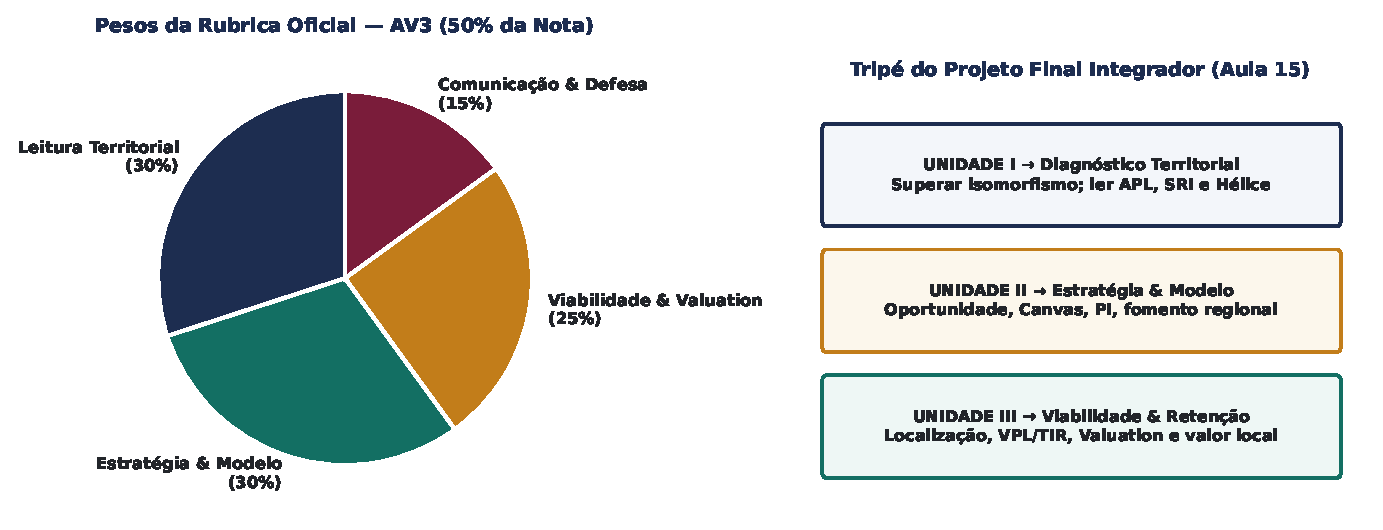
\includegraphics[width=0.94\textwidth]{figures/fig15_projeto_final_av3.pdf}
  \caption{Pesos oficiais da Rubrica AV3 (50\% da nota) e tripé de integração entre território, modelo de negócio e viabilidade econômico-financeira.}
  \label{fig:fig15_av3}
\end{figure}

A Tabela~\ref{tab:rubrica_av3} detalha os níveis de desempenho esperados em cada dimensão da rubrica oficial.

\begin{table}[H]
\centering
\caption{Matriz Oficial de Avaliação do Projeto Final Integrador (AV3).}
\label{tab:rubrica_av3}
\renewcommand{\arraystretch}{1.22}
\footnotesize
\begin{tabularx}{\textwidth}{@{}p{2.7cm} c >{\raggedright\arraybackslash}X >{\raggedright\arraybackslash}X@{}}
  \toprule
  \rowcolor{etIndigo}
  \textcolor{white}{\bfseries Dimensão} & \textcolor{white}{\bfseries Peso} & \textcolor{white}{\bfseries Padrão Insuficiente / Regular ($0{,}0$–$6{,}9$)} & \textcolor{white}{\bfseries Padrão Bom / Excelente ($7{,}0$–$10{,}0$)} \\
  \midrule
  \textbf{1. Leitura Territorial e Ecossistêmica ($L_T$)} & \textbf{30\%} & Descrição genérica da região; importação acrítica de modelos externos (isomorfismo); ausência de dados de APL, SRI ou atores da Hélice. & Diagnóstico territorial com dados empíricos; articulação precisa com APL/SRI, Hélice Quádrupla/Quíntupla, proximidades de Boschma e impacto socioambiental. \\
  \rowcolor{bgGray}
  \textbf{2. Estratégia, Oportunidade e Modelo ($E_M$)} & \textbf{30\%} & Oportunidade vaga sem TAM/SAM/SOM; Canvas desconectado do problema; omissão de PI e de fontes reais de fomento regional. & Funil TAM/SAM/SOM auditável; Canvas coerente com métricas (LTV/CAC, Burn/Runway); estratégia clara de PI e captação (FINEP, BNDES, BNB, FAPESB). \\
  \textbf{3. Viabilidade e \textit{Valuation} ($V_F$)} & \textbf{25\%} & Escolha locacional intuitiva; fluxo de caixa com premissas sem lastro; ausência de TMA/WACC, VPL, TIR ou confusão entre EV e Equity. & Matriz locacional ponderada; FCL consistente com CAPEX/OPEX; cálculo correto de VPL, TIR, Payback, WACC, \textit{Valuation} (FCD/VC) e análise de sensibilidade/IRV. \\
  \rowcolor{bgGray}
  \textbf{4. Comunicação e Defesa Oral ($C_D$)} & \textbf{15\%} & Slides poluídos, extrapolação severa dos 20 min, leitura integral de texto e respostas defensivas ou imprecisas na arguição. & Síntese visual limpa em 10 slides dentro dos 20 min; domínio conceitual e numérico na arguição de 10 min, reconhecendo limites e premissas. \\
  \bottomrule
\end{tabularx}
\end{table}

\subsection{Roteiro Estruturado de Apresentação em 10 Slides (20 min + 10 min)}

Para cumprir rigorosamente o tempo de 20 minutos, recomenda-se a cadência média de 2 minutos por slide, reservando 10 minutos finais para a arguição técnica da banca:

\begin{table}[H]
\centering
\caption{Roteiro padrão de 10 slides para a Defesa Oral da AV3 (20 minutos).}
\label{tab:roteiro_10_slides}
\renewcommand{\arraystretch}{1.18}
\footnotesize
\begin{tabularx}{\textwidth}{@{}c p{4.0cm} c >{\raggedright\arraybackslash}X@{}}
  \toprule
  \rowcolor{etTeal}
  \textcolor{white}{\bfseries Slide} & \textcolor{white}{\bfseries Título Funcional} & \textcolor{white}{\bfseries Tempo} & \textcolor{white}{\bfseries Conteúdo Essencial e Evidências Exigidas} \\
  \midrule
  \textbf{1} & Título, Equipe e Recorte Territorial & 1 min & Nome do projeto/empreendimento, território-alvo (município/região), problema central e vínculo com APL/SRI. \\
  \rowcolor{bgGray}
  \textbf{2} & Diagnóstico Territorial e Ecossistêmico & 2 min & Dados do território, estrutura de mercado ($\text{HHI}$ ou densidade produtiva), gargalos e atores da Hélice Quádrupla/Quíntupla. \\
  \textbf{3} & Oportunidade e Enquadramento Tecnológico & 2 min & Origem da oportunidade (\textit{discovery}/\textit{creation}), maturidade tecnológica ($\text{TRL}$), solução proposta e diferencial frente a incumbentes. \\
  \rowcolor{bgGray}
  \textbf{4} & Mercado (\text{TAM/SAM/SOM}) e Impacto & 2 min & Funil quantificado de mercado alcançável e, quando aplicável, Teoria da Mudança (insumos, produtos, resultados, impacto). \\
  \textbf{5} & Modelo de Negócio e Tração & 2 min & Síntese do \textit{Canvas} (proposta de valor, segmentos, receitas/custos) e métricas unitárias ($\text{CAC}$, $\text{LTV}$, $\text{LTV/CAC}$). \\
  \rowcolor{bgGray}
  \textbf{6} & Propriedade Intelectual e Fomento & 2 min & Estratégia de PI (patente, registro, IG, Tecnologia Social) e escada de capital (subvenção FAPESB/FINEP, crédito BNB/BNDES). \\
  \textbf{7} & Decisão Locacional Multicritério & 2 min & Tabela resumida da Matriz Locacional comparando alternativas municipais/distritais e justificando os pesos adotados. \\
  \rowcolor{bgGray}
  \textbf{8} & Viabilidade Econômico-Financeira & 3 min & $\text{CAPEX}$, $\text{OPEX}$, $\text{FCL}$ projetado, $\text{TMA}/\text{WACC}$, $\text{VPL}$, $\text{TIR}$/\text{MTIR}, \textit{Payback} Descontado e análise de sensibilidade. \\
  \textbf{9} & \textit{Valuation} e Retenção Territorial & 2 min & Estimativa de $\text{EV}$ e \textit{Equity Value} (FCD ou VC), diluição (se houver rodada) e cálculo do $\text{IRV}$ / externalidades locais. \\
  \rowcolor{bgGray}
  \textbf{10} & Riscos, Cronograma e Encaminhamentos & 2 min & Principais riscos técnicos/territoriais com mitigação, marcos de 12–24 meses e agenda de publicação ou implantação. \\
  \bottomrule
\end{tabularx}
\end{table}

\subsection{Encaminhamentos para Publicação Científica (ANPUR, ENANPAD e ENGEMA)}

No âmbito da pós-graduação (PLANTERR/UEFS), o Projeto Final Integrador não deve se encerrar na defesa em sala, pois um relatório técnico bem estruturado contém os elementos centrais para gerar um artigo científico competitivo nos principais fóruns brasileiros de Planejamento Urbano e Regional, Administração e Sustentabilidade.

No \textbf{ENANPUR (Encontro Nacional da ANPUR) e na Revista Brasileira de Estudos Urbanos e Regionais (RBEUR)}, privilegiam-se o recorte espacial, a economia política do território, a governança de APLs e SRIs, as desigualdades regionais e a crítica ao isomorfismo de políticas de CT\&I; para esse público, o foco do artigo deve enfatizar a leitura territorial ($L_T$), a distribuição espacial da renda e os limites institucionais do ecossistema local. Já o \textbf{ENANPAD (Divisões de Estratégia, Empreendedorismo e Gestão Pública/Inovação) e periódicos como \textit{Organizações \& Sociedade (O\&S)}} valorizam a articulação entre teoria da firma e ecossistemas (Shane \& Venkataraman, Sarasvathy, Stam, Teece/Chesbrough), modelos de negócio, \textit{spin-offs} acadêmicas e mensuração rigorosa de desempenho e \textit{Valuation}. Por sua vez, o \textbf{ENGEMA (Encontro Internacional sobre Gestão Empresarial e Meio Ambiente)} acolhe estudos sobre negócios de impacto socioambiental, bioeconomia, Tecnologia Social, Indicações Geográficas sustentáveis, transição energética e métricas de retenção territorial e ambiental.

\begin{boxConceito}[Da Proposta Aplicada ao Artigo Científico Auditável]
Para converter o projeto da AV3 em artigo publicável, realize quatro ajustes metodológicos: (1) substitua a linguagem prescritiva de plano de negócios por uma \textbf{pergunta de pesquisa} explícita (por exemplo, ``Em que medida o acoplamento a um APL regional altera a viabilidade e a retenção de valor de uma \textit{spin-off} de base tecnológica?''); (2) explicite o \textbf{desenho metodológico} (estudo de caso único/múltiplo, modelagem multicritério ou simulação de FCD com análise de sensibilidade); (3) documente as fontes primárias e secundárias (IBGE, RAIS, INPI, editais, entrevistas); e (4) discuta \textbf{achados e limites} com modéstia epistêmica, evitando generalizações para territórios distintos sem controle contextual.
\end{boxConceito}

\etapa{4}{Estudos de Caso e Exemplos Resolvidos Passo a Passo}

\begin{boxExemplo}{15.1}{Cálculo da Nota na Rubrica AV3 e Planejamento da Média Final}
\passoEnunciado{Um mestrando do PLANTERR/UEFS obteve nota $8{,}2$ na AV1 (peso $30\%$) e $7{,}5$ na AV2 (peso $20\%$). Na defesa oral do Projeto Final Integrador (AV3, peso $50\%$), a banca atribuiu as seguintes notas parciais: Leitura Territorial $L_T = 8{,}5$; Estratégia e Modelo $E_M = 8{,}0$; Viabilidade e \textit{Valuation} $V_F = 8{,}8$; Comunicação e Defesa $C_D = 9{,}0$.}
\passoDados{$\text{AV1} = 8{,}2$; $\text{AV2} = 7{,}5$; $L_T = 8{,}5$; $E_M = 8{,}0$; $V_F = 8{,}8$; $C_D = 9{,}0$. Pesos da rubrica AV3: $0{,}30$; $0{,}30$; $0{,}25$; $0{,}15$. Pesos da disciplina: $0{,}30$; $0{,}20$; $0{,}50$.}
\passoPedido{Calcular a nota $N_{\text{AV3}}$, a Média Final $M_F$ e determinar qual teria sido a nota mínima necessária na AV3 para o discente alcançar $M_F = 8{,}0$.}
\passoMetodo{Aplicação direta das médias ponderadas da Rubrica Oficial AV3 e do Sistema de Avaliação da disciplina.}
\passoContas{
1. Cálculo de $N_{\text{AV3}}$:
\[
N_{\text{AV3}} = 0{,}30(8{,}5) + 0{,}30(8{,}0) + 0{,}25(8{,}8) + 0{,}15(9{,}0)
\]
\[
N_{\text{AV3}} = 2{,}55 + 2{,}40 + 2{,}20 + 1{,}35 = 8{,}50
\]
2. Cálculo da Média Final ($M_F$):
\[
M_F = 0{,}30(8{,}2) + 0{,}20(7{,}5) + 0{,}50(8{,}50) = 2{,}46 + 1{,}50 + 4{,}25 = 8{,}21
\]
3. Nota mínima na AV3 para atingir $M_F = 8{,}00$:
\[
0{,}30(8{,}2) + 0{,}20(7{,}5) + 0{,}50\,N_{\text{AV3,mín}} = 8{,}00 \implies 3{,}96 + 0{,}50\,N_{\text{AV3,mín}} = 8{,}00
\]
\[
N_{\text{AV3,mín}} = \frac{8{,}00 - 3{,}96}{0{,}50} = \frac{4{,}04}{0{,}50} = 8{,}08
\]
}
\passoResposta{$N_{\text{AV3}} = 8{,}50$; $M_F = 8{,}21$; nota mínima na AV3 para alcançar $M_F = 8{,}00$ era $8{,}08$.}
\passoVerificacao{Como a AV3 responde por metade da média final, um desempenho equilibrado acima de $8{,}0$ em todos os blocos garantiu folga sobre a meta, com destaque para a robustez em viabilidade financeira ($8{,}8$) e defesa oral ($9{,}0$).}
\end{boxExemplo}

\begin{boxExemplo}{15.2}{Integração Territorial-Financeira de uma \textit{Spin-off} de Bioeconomia no Semiárido}
\passoEnunciado{Uma \textit{spin-off} originada na UEFS desenvolve biopolímeros a partir de subprodutos do sisal no Território do Sisal / Portal do Sertão (BA). O projeto prevê investimento inicial ($\text{CAPEX}_0$) de $\reais{350.000}$, com Fluxos de Caixa Livres anuais de $\reais{130.000}$ (Ano 1), $\reais{170.000}$ (Ano 2) e $\reais{210.000}$ (Ano 3), descontados a uma $\text{TMA}$ de $12\%$ ao ano. Do desembolso operacional anual médio de $\reais{400.000}$, estima-se que $\reais{272.000}$ sejam pagos a cooperativas locais de matéria-prima e mão de obra técnica residente na região.}
\passoDados{$I_0 = \reais{350.000}$; $\text{FCL}_1 = \reais{130.000}$; $\text{FCL}_2 = \reais{170.000}$; $\text{FCL}_3 = \reais{210.000}$; $i = 12\%\text{ a.a.}$; gasto local $= \reais{272.000}$ sobre desembolso operacional total de $\reais{400.000}$.}
\passoPedido{Calcular o $\text{VPL}$, o \textit{Payback} Descontado, a $\text{TIR}$ aproximada e o Índice de Retenção Territorial de Valor ($\text{IRV}$).}
\passoMetodo{Fluxo de Caixa Descontado (Unidade III) integrado ao indicador de retenção territorial ($\text{IRV}$).}
\passoContas{
1. Valor Presente de cada fluxo a $i = 12\%$ a.a.:
\[
\text{VP}_1 = \frac{130.000}{1{,}12^1} = \frac{130.000}{1{,}12} = \reais{116.071{,}43}
\]
\[
\text{VP}_2 = \frac{170.000}{1{,}12^2} = \frac{170.000}{1{,}2544} = \reais{135.522{,}96}
\]
\[
\text{VP}_3 = \frac{210.000}{1{,}12^3} = \frac{210.000}{1{,}404928} = \reais{149.473{,}85}
\]
2. Cálculo do $\text{VPL}$:
\[
\text{VPL} = -350.000 + 116.071{,}43 + 135.522{,}96 + 149.473{,}85 = \reais{51.068{,}24}
\]
3. Cálculo do \textit{Payback} Descontado ($PB_d$):
\begin{itemize}[leftmargin=1.4em]
  \item Saldo acumulado em $t = 1$: $-350.000 + 116.071{,}43 = -\reais{233.928{,}57}$.
  \item Saldo acumulado em $t = 2$: $-233.928{,}57 + 135.522{,}96 = -\reais{98.405{,}61}$.
  \item No Ano 3, recupera-se o saldo negativo restante:
  \[
  PB_d = 2 + \frac{98.405{,}61}{149.473{,}85} = 2 + 0{,}6583 \approx 2{,}66\text{ anos}
  \]
\end{itemize}
4. Verificação da $\text{TIR}$: testando $i = 19{,}65\%$ a.a., tem-se:
\[
\frac{130.000}{1{,}1965} + \frac{170.000}{1{,}1965^2} + \frac{210.000}{1{,}1965^3} = 108.650{,}23 + 118.747{,}23 + 122.601{,}11 \approx \reais{349.998{,}57} \implies \text{TIR} \approx 19{,}65\%\text{ a.a.}
\]
5. Cálculo do $\text{IRV}$:
\[
\text{IRV} = \frac{272.000}{400.000} = 0{,}68 = 68\%
\]
}
\passoResposta{$\text{VPL} = \reais{51.068{,}24}$; $PB_d \approx 2{,}66\text{ anos}$; $\text{TIR} \approx 19{,}65\%\text{ a.a.}$; $\text{IRV} = 68\%$.}
\passoVerificacao{O projeto é financeiramente viável ($\text{VPL} > 0$ e $\text{TIR} = 19{,}65\% > \text{TMA} = 12\%$) e apresenta elevado enraizamento produtivo, mantendo $68\%$ do dispêndio operacional no próprio território sisaleiro.}
\end{boxExemplo}

\begin{boxExemplo}{15.3}{Decisão Locacional Multicritério e Método de \textit{Venture Capital} (VC)}
\passoEnunciado{Uma \textit{cleantech} baiana de microgeração solar comunitária avalia três municípios (Feira de Santana, Alagoinhas e Juazeiro) segundo quatro critérios ponderados: (C1) Proximidade ao APL e universidade/ICT (peso $0{,}35$); (C2) Infraestrutura logística e energia (peso $0{,}25$); (C3) Incentivos fiscais e fomento estadual/BNB (peso $0{,}25$); e (C4) Disponibilidade de mão de obra técnica (peso $0{,}15$). As notas ($0$ a $10$) foram: Feira de Santana $(9; 8; 7; 8)$, Alagoinhas $(7; 7; 8; 7)$ e Juazeiro $(8; 6; 9; 9)$. Para financiar a planta piloto no município vencedor, a empresa negocia um aporte de $\reais{600.000}$ com um fundo de impacto que exige retorno-alvo de $40\%$ ao ano em 4 anos, projetando valor de saída de $\reais{9.600.000}$ no Ano 4.}
\passoDados{Pesos $w = (0{,}35; 0{,}25; 0{,}25; 0{,}15)$; notas das três cidades; aporte $I = \reais{600.000}$; $k_{\text{VC}} = 40\%\text{ a.a.}$; $T = 4$ anos; $V_{\text{saída}} = \reais{9.600.000}$.}
\passoPedido{Definir o município vencedor pela Matriz Locacional e calcular o \textit{Valuation Post-Money}, o \textit{Valuation Pre-Money} e a participação societária (diluição) cedida ao fundo.}
\passoMetodo{Média ponderada da Matriz Locacional (Cap.\ 12) combinada ao Método de \textit{Venture Capital} (Cap.\ 14).}
\passoContas{
1. Pontuação na Matriz Locacional ($S_j = \sum w_i n_{ij}$):
\begin{itemize}[leftmargin=1.4em]
  \item Feira de Santana: $S_{\text{FSA}} = 0{,}35(9) + 0{,}25(8) + 0{,}25(7) + 0{,}15(8) = 3{,}15 + 2{,}00 + 1{,}75 + 1{,}20 = 8{,}10$.
  \item Alagoinhas: $S_{\text{ALA}} = 0{,}35(7) + 0{,}25(7) + 0{,}25(8) + 0{,}15(7) = 2{,}45 + 1{,}75 + 2{,}00 + 1{,}05 = 7{,}25$.
  \item Juazeiro: $S_{\text{JUA}} = 0{,}35(8) + 0{,}25(6) + 0{,}25(9) + 0{,}15(9) = 2{,}80 + 1{,}50 + 2{,}25 + 1{,}35 = 7{,}90$.
\end{itemize}
Logo, \textbf{Feira de Santana} obtém a maior pontuação ($8{,}10$).

2. Cálculo do \textit{Valuation} pelo Método de \textit{Venture Capital}:
\[
V_{\text{Post-Money}} = \frac{V_{\text{saída}}}{(1 + k_{\text{VC}})^T} = \frac{9.600.000}{(1{,}40)^4} = \frac{9.600.000}{3{,}8416} = \reais{2.498.958{,}77}
\]
\[
V_{\text{Pre-Money}} = V_{\text{Post-Money}} - \text{Aporte} = 2.498.958{,}77 - 600.000{,}00 = \reais{1.898.958{,}77}
\]
\[
\text{Participação do Fundo (Diluição)} = \frac{600.000{,}00}{2.498.958{,}77} \approx 0{,}2401 = 24{,}01\%
\]
}
\passoResposta{Município selecionado: Feira de Santana ($8{,}10$); $V_{\text{Post-Money}} = \reais{2.498.958{,}77}$; $V_{\text{Pre-Money}} = \reais{1.898.958{,}77}$; diluição de $24{,}01\%$.}
\passoVerificacao{Feira de Santana vence pela força da proximidade com ICTs e logística central, embora Juazeiro fique próximo ($7{,}90$) devido aos incentivos e à insolação. A diluição de $24{,}01\%$ está dentro da faixa usual ($15\%$ a $30\%$) para rodadas \textit{Seed}, preservando o controle dos fundadores e a governança contra \textit{mission drift}.}
\end{boxExemplo}

\begin{boxExemplo}{15.4}{Diagnóstico Comparativo de Dois Projetos na Banca AV3}
\passoEnunciado{Durante o Seminário Final (AV3), dois projetos disputam indicação para incubação tecnológica. O \textbf{Projeto A} propõe um aplicativo genérico de entregas urbanas sem vínculo com cadeias produtivas locais, recebendo $L_T = 4{,}5$, $E_M = 7{,}5$, $V_F = 7{,}0$ e $C_D = 8{,}0$. O \textbf{Projeto B} propõe uma plataforma de rastreabilidade e certificação digital acoplada a uma Indicação Geográfica de cafés especiais da Chapada Diamantina, recebendo $L_T = 9{,}0$, $E_M = 8{,}5$, $V_F = 8{,}2$ e $C_D = 8{,}0$.}
\passoDados{Notas de A: $(4{,}5; 7{,}5; 7{,}0; 8{,}0)$. Notas de B: $(9{,}0; 8{,}5; 8{,}2; 8{,}0)$. Pesos AV3: $(0{,}30; 0{,}30; 0{,}25; 0{,}15)$.}
\passoPedido{Calcular a nota final $N_{\text{AV3}}$ de ambos os projetos, a diferença absoluta entre eles e identificar qual dimensão explica a maior parcela dessa diferença.}
\passoMetodo{Aplicação da Rubrica Oficial AV3 com decomposição das contribuições ponderadas.}
\passoContas{
1. Projeto A:
\[
N_A = 0{,}30(4{,}5) + 0{,}30(7{,}5) + 0{,}25(7{,}0) + 0{,}15(8{,}0) = 1{,}35 + 2{,}25 + 1{,}75 + 1{,}20 = 6{,}55
\]
2. Projeto B:
\[
N_B = 0{,}30(9{,}0) + 0{,}30(8{,}5) + 0{,}25(8{,}2) + 0{,}15(8{,}0) = 2{,}70 + 2{,}55 + 2{,}05 + 1{,}20 = 8{,}50
\]
3. Diferença total e decomposição:
\[
N_B - N_A = 8{,}50 - 6{,}55 = 1{,}95\text{ ponto}
\]
Contribuição por critério:
\begin{itemize}[leftmargin=1.4em]
  \item $\Delta L_T = 0{,}30(9{,}0 - 4{,}5) = 1{,}35$ ponto ($69{,}2\%$ da diferença total);
  \item $\Delta E_M = 0{,}30(8{,}5 - 7{,}5) = 0{,}30$ ponto;
  \item $\Delta V_F = 0{,}25(8{,}2 - 7{,}0) = 0{,}30$ ponto;
  \item $\Delta C_D = 0{,}15(8{,}0 - 8{,}0) = 0{,}00$ ponto.
\end{itemize}
}
\passoResposta{$N_A = 6{,}55$; $N_B = 8{,}50$; diferença de $1{,}95$ ponto, explicada em $69{,}2\%$ pela Leitura Territorial ($L_T$).}
\passoVerificacao{Mesmo com comunicação oral idêntica ($8{,}0$) e estratégia razoável, o isomorfismo territorial penalizou severamente o Projeto A, mostrando que o alinhamento com ativos territoriais específicos (como uma IG) é decisivo na AV3.}
\end{boxExemplo}

\begin{boxExemplo}{15.5}{Conversão do Projeto AV3 em Artigo Científico: Desconcentração de Mercado ($\text{HHI}$)}
\passoEnunciado{Para submeter seu Projeto AV3 ao ENANPUR/ENANPAD, uma pesquisadora avalia o impacto competitivo da entrada de uma cooperativa de base tecnológica em um mercado regional de beneficiamento agrícola anteriormente concentrado em quatro empresas com participações de $40\%$, $30\%$, $20\%$ e $10\%$. Após dois anos de operação apoiada por edital da FAPESB, a cooperativa captura $20\%$ do mercado, reduzindo proporcionalmente a fatia das incumbentes para $32\%$, $24\%$, $16\%$ e $8\%$.}
\passoDados{Cenário inicial: $s = (40, 30, 20, 10)$. Cenário pós-entrada: $s' = (32, 24, 16, 8, 20)$.}
\passoPedido{Calcular o Índice Herfindahl-Hirschman ($\text{HHI}$) antes e depois da entrada da cooperativa e classificar a mudança estrutural para inclusão na seção de resultados do artigo.}
\passoMetodo{Cálculo de $\text{HHI} = \sum_{i=1}^{n} s_i^2$ (escala $0$ a $10.000$) e critérios usuais de concentração (desconcentrado $< 1.500$; moderadamente concentrado $1.500$–$2.500$; altamente concentrado $> 2.500$).}
\passoContas{
1. $\text{HHI}$ antes da entrada:
\[
\text{HHI}_{\text{antes}} = 40^2 + 30^2 + 20^2 + 10^2 = 1.600 + 900 + 400 + 100 = 3.000
\]
2. $\text{HHI}$ após a entrada da cooperativa tecnológica:
\[
\text{HHI}_{\text{depois}} = 32^2 + 24^2 + 16^2 + 8^2 + 20^2 = 1.024 + 576 + 256 + 64 + 400 = 2.320
\]
3. Redução absoluta:
\[
\Delta\text{HHI} = 3.000 - 2.320 = 680\text{ pontos}
\]
}
\passoResposta{$\text{HHI}_{\text{antes}} = 3.000$ (altamente concentrado); $\text{HHI}_{\text{depois}} = 2.320$ (moderadamente concentrado); redução de $680$ pontos.}
\passoVerificacao{O resultado quantitativo oferece evidência auditável para o artigo científico: a inovação associativa não apenas viabilizou uma nova firma, mas reduziu a concentração oligopolística regional de alta para moderada.}
\end{boxExemplo}

\etapa{5}{Armadilhas Conceituais e Erros Mais Comuns na AV3}

\begin{boxErro}[Erro 1: Isomorfismo Institucional (``Vale do Silício de Papel'')]
Propor incubadoras, \textit{hubs} digitais ou plataformas genéricas sem demonstrar conexão com a base produtiva, a densidade institucional ou os gargalos reais do território estudado. Na Rubrica AV3, esse descolamento derruba a nota de Leitura Territorial ($L_T$, $30\%$ do peso) mesmo que os slides sejam visualmente atraentes.
\end{boxErro}

\begin{boxErro}[Erro 2: Desconexão entre TAM/SAM/SOM, Canvas e Fluxo de Caixa]
Apresentar um $\text{SOM}$ milionário no Slide 4 e, no Slide 8, projetar receitas ou custos operacionais incompatíveis com o número de clientes alcançáveis, com o $\text{CAC}$ ou com a capacidade instalada definida no $\text{CAPEX}$. Toda premissa financeira deve derivar diretamente do modelo de negócio e do funil de mercado.
\end{boxErro}

\begin{boxErro}[Erro 3: Omitir Custo de Oportunidade ou Confundir EV com Equity Value]
Avaliar o projeto somando fluxos de caixa nominais sem desconto pela $\text{TMA}/\text{WACC}$, ou apresentar o \textit{Enterprise Value} ($\text{EV}$) como se fosse o valor líquido disponível aos sócios, esquecendo de subtrair a dívida bruta e somar o caixa disponível para obter o \textit{Equity Value}.
\end{boxErro}

\begin{boxErro}[Erro 4: Desequilíbrio de Tempo na Defesa Oral (10 Slides em 20 min)]
Consumir $12$ minutos na contextualização teórica inicial (Slides 1 a 3) e acelerar ou suprimir os slides de Decisão Locacional, Viabilidade Financeira e \textit{Valuation} (Slides 7 a 9). A banca avalia a síntese integradora; cada bloco exige seu tempo proporcional.
\end{boxErro}

\etapa{6}{Exercícios Propostos (3 Níveis)}

\subsection*{Nível 1: Básico (Rubrica, Média Final e Retenção Territorial)}

\begin{enumerate}[leftmargin=1.5em, itemsep=4pt]
  \item Um projeto obteve na banca AV3 as notas $L_T = 8{,}0$, $E_M = 9{,}0$, $V_F = 7{,}0$ e $C_D = 8{,}0$. Calcule a nota final $N_{\text{AV3}}$ utilizando os pesos oficiais da rubrica.
  \espacoResolucao[1.8cm]

  \item Considere um discente com $\text{AV1} = 7{,}0$, $\text{AV2} = 8{,}0$ e $N_{\text{AV3}} = 8{,}6$. Determine sua Média Final ($M_F$) na disciplina.
  \espacoResolucao[1.8cm]

  \item Uma estudante obteve $\text{AV1} = 6{,}0$ e $\text{AV2} = 7{,}0$. Qual deve ser a nota mínima na AV3 para que sua Média Final seja exatamente $7{,}0$?
  \espacoResolucao[1.8cm]

  \item Um empreendimento agroindustrial tecnológico gera desembolso operacional anual de $\reais{600.000}$, dos quais $\reais{420.000}$ correspondem a salários locais e compra de insumos de produtores do próprio território. Calcule o Índice de Retenção Territorial de Valor ($\text{IRV}$).
  \espacoResolucao[1.8cm]

  \item Na defesa oficial da AV3 ($20$ min de exposição + $10$ min de arguição), qual o tempo médio disponível por slide em um roteiro de $10$ slides e qual percentual do tempo total da sessão é dedicado à arguição da banca?
  \espacoResolucao[1.8cm]
\end{enumerate}

\subsection*{Nível 2: Intermediário (Mercado, Tração e Decisão Locacional)}

\begin{enumerate}[leftmargin=1.5em, itemsep=4pt, resume]
  \item Em um projeto de saúde digital para municípios do semiárido, o mercado total endereçável ($\text{TAM}$) é de $\reais{50.000.000}$/ano. O mercado endereçável acessível ($\text{SAM}$) corresponde a $20\%$ do $\text{TAM}$, e a meta realista de captura em 3 anos ($\text{SOM}$) é de $8\%$ do $\text{SAM}$. Calcule $\text{SAM}$ e $\text{SOM}$ em reais.
  \espacoResolucao[2.0cm]

  \item Uma edtech regional cobra assinatura mensal de $\reais{400}$, possui margem de contribuição de $60\%$, retenção média de $15$ meses e custo de aquisição de cliente ($\text{CAC}$) de $\reais{1.200}$. Calcule o $\text{LTV}$ e a razão $\text{LTV/CAC}$, interpretando o resultado.
  \espacoResolucao[2.0cm]

  \item Uma \textit{spin-off} possui $\reais{240.000}$ em caixa, queima bruta mensal (\textit{gross burn}) de $\reais{55.000}$ e receita mensal recorrente de $\reais{25.000}$. Calcule o \textit{net burn} e o \textit{runway} em meses.
  \espacoResolucao[2.0cm]

  \item Uma matriz locacional utiliza três critérios: C1 (peso $0{,}40$), C2 (peso $0{,}35$) e C3 (peso $0{,}25$). O Município A recebeu notas $(8; 7; 6)$ e o Município B recebeu $(6; 9; 8)$. Qual município deve ser escolhido?
  \espacoResolucao[2.0cm]

  \item Um laboratório de prototipagem territorial tem custos fixos mensais de $\reais{36.000}$, preço médio por serviço de $\reais{180}$ e custo variável unitário de $\reais{100}$. Calcule o Ponto de Equilíbrio contábil mensal em unidades de serviço.
  \espacoResolucao[2.0cm]
\end{enumerate}

\subsection*{Nível 3: Avançado (Viabilidade, Valuation e Simulação de Banca)}

\begin{enumerate}[leftmargin=1.5em, itemsep=4pt, resume]
  \item Um projeto apresenta $\text{CAPEX}_0 = \reais{200.000}$ e fluxos líquidos anuais de $\reais{90.000}$ (Ano 1), $\reais{100.000}$ (Ano 2) e $\reais{110.000}$ (Ano 3), com $\text{TMA} = 10\%$ a.a. Calcule o $\text{VPL}$ e o \textit{Payback} Descontado.
  \espacoResolucao[2.4cm]

  \item Uma empresa de base tecnológica financia seus ativos com $\reais{600.000}$ de capital próprio ($K_e = 16\%$ a.a.) e $\reais{400.000}$ de dívida ($K_d = 10\%$ a.a.), sob alíquota de imposto de renda $T = 34\%$. Calcule o $\text{WACC}$.
  \espacoResolucao[2.2cm]

  \item Um empreendimento projeta $\text{VP}(\text{FCL}_{1..3}) = \reais{320.000}$ e $\text{FCL}_3 = \reais{150.000}$. Após o Ano 3, estima-se crescimento perpétuo $g = 3\%$ a.a. com $\text{WACC} = 13\%$ a.a. Sabendo que a empresa tem dívida bruta de $\reais{180.000}$ e caixa de $\reais{50.000}$, calcule o Valor Terminal ($VT$), o $\text{EV}$ e o \textit{Equity Value}.
  \espacoResolucao[2.5cm]

  \item Um fundo de \textit{Venture Capital} exige retorno de $50\%$ a.a. em $3$ anos para aportar $\reais{500.000}$ em uma \textit{agtech}, cujo valor de saída projetado no Ano 3 é de $\reais{8.000.000}$. Calcule o \textit{Post-Money}, o \textit{Pre-Money} e a diluição do empreendedor.
  \espacoResolucao[2.4cm]

  \item Na pré-banca da AV3, um grupo obteve $L_T = 6{,}0$. Após incorporar dados de $\text{HHI}$, matriz locacional e vínculos com o APL local, elevou esse único critério para $L_T = 9{,}0$, mantendo os demais inalterados. Qual foi o ganho absoluto na nota $N_{\text{AV3}}$ e na Média Final ($M_F$)?
  \espacoResolucao[2.0cm]
\end{enumerate}

\etapa{7}{Questões Autorais Estilo ANPAD / POSCOMP / Concursos de CT\&I}

\begin{enumerate}[leftmargin=1.5em, itemsep=5pt]
  \item \textbf{(Estilo ANPAD / Planejamento Territorial)} Um consórcio intermunicipal no semiárido pretende implantar um polo de inovação em energias renováveis. Para evitar o chamado ``isomorfismo institucional'' na avaliação de projetos (critério de leitura territorial e ecossistêmica), a proposta deve priorizar:
  \begin{alternativas}
    \item A replicação integral do estatuto de parques tecnológicos metropolitanos sem adaptação às cadeias locais.
    \item O acoplamento da solução tecnológica às capacidades produtivas regionais, às ICTs próximas e aos atores da Hélice Quádrupla/Quíntupla.
    \item A substituição imediata de toda mão de obra local por consultorias externas permanentes de grandes centros.
    \item A exclusão de instrumentos públicos de fomento para operar exclusivamente com capital especulativo de curto prazo.
    \item A apresentação de projeções financeiras sem matriz locacional nem análise de retenção territorial de valor.
  \end{alternativas}

  \item \textbf{(Estilo Concursos de CT\&I / Fomento)} Na preparação de uma \textit{spin-off} acadêmica para defesa em banca de avaliação e submissão ao edital de subvenção econômica (FAPESB/FINEP), a articulação correta entre estratégia de mercado e engenharia financeira exige que:
  \begin{alternativas}
    \item O \textit{Business Model Canvas} seja elaborado após a definição do \textit{Valuation} terminal, independentemente do $\text{SOM}$.
    \item O $\text{VPL}$ seja calculado somando os fluxos nominais sem taxa de desconto, pois projetos de CT\&I não possuem custo de oportunidade.
    \item O funil $\text{TAM/SAM/SOM}$ sustente as premissas de receita do $\text{FCL}$, enquanto a $\text{TMA}$ ou $\text{WACC}$ desconte os fluxos futuros para aferir o $\text{VPL}$.
    \item O \textit{Enterprise Value} seja tratado como sinônimo exato de \textit{Equity Value}, mesmo na presença de endividamento bancário relevante.
    \item A proteção de Propriedade Intelectual seja adiada para depois da divulgação pública integral da tecnologia em congresso.
  \end{alternativas}

  \item \textbf{(Estilo POSCOMP / Gestão da Inovação)} Ao converter o relatório técnico de um projeto territorial em artigo científico para o ENANPUR, ENANPAD ou ENGEMA, o principal requisito metodológico que diferencia a publicação acadêmica do plano de negócios é:
  \begin{alternativas}
    \item A supressão de todas as equações financeiras e dados secundários para privilegiar apenas opiniões pessoais dos autores.
    \item A formulação de pergunta de pesquisa clara, explicitação do método auditável, documentação das fontes e discussão crítica dos limites do estudo.
    \item A garantia de que o artigo apresente $\text{VPL}$ positivo, independentemente da coerência das premissas territoriais.
    \item O uso exclusivo de referências estrangeiras recentes, omitindo marcos regulatórios brasileiros e autores de planejamento regional.
    \item A apresentação em formato de 10 slides sem revisão bibliográfica nem análise de sensibilidade.
  \end{alternativas}
\end{enumerate}

\begin{boxDica}[Contraponto Crítico e Prática Territorial (AV3)]
Mesmo quando um projeto apresenta $\text{VPL}$ positivo e $\text{LTV/CAC} > 3$, a banca do PLANTERR/UEFS examina \textbf{quem captura o valor gerado}. Projetos com alta rentabilidade privada podem produzir baixo desenvolvimento territorial se importarem todos os insumos tecnológicos e remeterem os lucros para fora da região. Por isso, combine sempre os indicadores financeiros clássicos com métricas de enraizamento ($\text{IRV}$, empregos qualificados locais, encadeamento com APLs e preservação socioambiental).
\end{boxDica}

\clearpage
\etapa{8}{Gabarito Integralmente Comentado}

\begin{boxGabarito}[Resolução Passo a Passo: Exercícios da Etapa 6]
\begin{enumerate}[leftmargin=1.5em, itemsep=4pt]
  \item $N_{\text{AV3}} = 0{,}30(8{,}0) + 0{,}30(9{,}0) + 0{,}25(7{,}0) + 0{,}15(8{,}0) = 2{,}40 + 2{,}70 + 1{,}75 + 1{,}20 = \mathbf{8{,}05}$.
  \item $M_F = 0{,}30(7{,}0) + 0{,}20(8{,}0) + 0{,}50(8{,}6) = 2{,}10 + 1{,}60 + 4{,}30 = \mathbf{8{,}00}$.
  \item $0{,}30(6{,}0) + 0{,}20(7{,}0) + 0{,}50\,N_{\text{AV3}} = 7{,}0 \implies 1{,}80 + 1{,}40 + 0{,}50\,N_{\text{AV3}} = 7{,}0 \implies N_{\text{AV3}} = \frac{3{,}80}{0{,}50} = \mathbf{7{,}60}$.
  \item $\text{IRV} = \frac{420.000}{600.000} = 0{,}70 = \mathbf{70\%}$.
  \item Tempo médio por slide: $\frac{20}{10} = \mathbf{2{,}0\text{ min/slide}}$. Proporção da arguição no tempo total ($30$ min): $\frac{10}{30} = \mathbf{33{,}33\%}$.
  \item $\text{SAM} = 0{,}20 \times 50.000.000 = \mathbf{\reais{10.000.000}}$/ano; $\text{SOM} = 0{,}08 \times 10.000.000 = \mathbf{\reais{800.000}}$/ano.
  \item $\text{LTV} = 400 \times 0{,}60 \times 15 = \mathbf{\reais{3.600}}$; $\text{LTV/CAC} = \frac{3.600}{1.200} = \mathbf{3{,}0}$ (limiar saudável de sustentabilidade comercial).
  \item $\text{Net Burn} = 55.000 - 25.000 = \mathbf{\reais{30.000}}$/mês; $\text{Runway} = \frac{240.000}{30.000} = \mathbf{8\text{ meses}}$.
  \item $S_A = 0{,}40(8) + 0{,}35(7) + 0{,}25(6) = 3{,}20 + 2{,}45 + 1{,}50 = 7{,}15$; $S_B = 0{,}40(6) + 0{,}35(9) + 0{,}25(8) = 2{,}40 + 3{,}15 + 2{,}00 = \mathbf{7{,}55}$. Escolhe-se o \textbf{Município B}.
  \item $Q_{\text{PE}} = \frac{36.000}{180 - 100} = \frac{36.000}{80} = \mathbf{450\text{ unidades/mês}}$.
  \item $\text{VP}_1 = \frac{90.000}{1{,}10} = 81.818{,}18$; $\text{VP}_2 = \frac{100.000}{1{,}21} = 82.644{,}63$; $\text{VP}_3 = \frac{110.000}{1{,}331} = 82.644{,}63$. $\text{VPL} = -200.000 + 81.818{,}18 + 82.644{,}63 + 82.644{,}63 = \mathbf{\reais{47.107{,}44}}$. Saldo em $t=2$: $-200.000 + 81.818{,}18 + 82.644{,}63 = -35.537{,}19$. $PB_d = 2 + \frac{35.537{,}19}{82.644{,}63} \approx \mathbf{2{,}43\text{ anos}}$.
  \item Pesos: $w_E = \frac{600}{1.000} = 0{,}60$; $w_D = \frac{400}{1.000} = 0{,}40$. $\text{WACC} = 0{,}60(0{,}16) + 0{,}40(0{,}10)(1 - 0{,}34) = 0{,}096 + 0{,}0264 = 0{,}1224 = \mathbf{12{,}24\%\text{ a.a.}}$.
  \item $VT = \frac{150.000 \times 1{,}03}{0{,}13 - 0{,}03} = \frac{154.500}{0{,}10} = \mathbf{\reais{1.545.000}}$. $\text{VP}(VT) = \frac{1.545.000}{1{,}13^3} = \frac{1.545.000}{1{,}442897} = \reais{1.070.762{,}50}$. $\text{EV} = 320.000 + 1.070.762{,}50 = \mathbf{\reais{1.390.762{,}50}}$. $\text{Equity Value} = 1.390.762{,}50 - 180.000 + 50.000 = \mathbf{\reais{1.260.762{,}50}}$.
  \item $V_{\text{Post}} = \frac{8.000.000}{1{,}50^3} = \frac{8.000.000}{3{,}375} = \mathbf{\reais{2.370.370{,}37}}$; $V_{\text{Pre}} = 2.370.370{,}37 - 500.000 = \mathbf{\reais{1.870.370{,}37}}$; Diluição $= \frac{500.000}{2.370.370{,}37} \approx \mathbf{21{,}09\%}$.
  \item Ganho na AV3: $\Delta N_{\text{AV3}} = 0{,}30(9{,}0 - 6{,}0) = \mathbf{+0{,}90\text{ ponto}}$. Ganho na Média Final: $\Delta M_F = 0{,}50 \times 0{,}90 = \mathbf{+0{,}45\text{ ponto}}$.
\end{enumerate}
\end{boxGabarito}

\begin{boxGabarito}[Resolução Comentada: Questões da Etapa 7]
\begin{itemize}[leftmargin=1.4em, itemsep=3pt]
  \item \textbf{Questão 1 (Alternativa B):} A superação do isomorfismo exige enraizamento nas capacidades regionais e articulação entre universidade, empresa, governo e sociedade/ambiente (Hélice Quádrupla/Quíntupla).
  \item \textbf{Questão 2 (Alternativa C):} Há encadeamento causal obrigatório entre o mercado alcançável ($\text{SOM}$), o $\text{FCL}$ projetado e o desconto pela $\text{TMA}/\text{WACC}$ para aferição do $\text{VPL}$.
  \item \textbf{Questão 3 (Alternativa B):} A publicação científica em ANPUR, ENANPAD ou ENGEMA requer pergunta de pesquisa, método reprodutível, fontes documentadas e delimitação crítica de alcance e limites.
\end{itemize}
\end{boxGabarito}

\begin{boxResumo}
\begin{itemize}[leftmargin=1.4em, itemsep=2pt]
  \item O Projeto Final Integrador (\textbf{AV3, 50\%}) sintetiza Leitura Territorial ($30\%$), Estratégia e Modelo ($30\%$), Viabilidade e \textit{Valuation} ($25\%$) e Comunicação/Defesa ($15\%$).
  \item A defesa oral dura \textbf{20 minutos} (roteiro em 10 slides) seguidos de \textbf{10 minutos de arguição}.
  \item A coerência do projeto exige amarração numérica: $\text{SOM} \to \text{Receitas/FCL} \to \text{VPL/TIR/Valuation} \to \text{IRV}$.
  \item O mesmo arcabouço empírico e quantitativo pode ser convertido em artigo científico para ENANPUR/RBEUR, ENANPAD/O\&S ou ENGEMA mediante explicitação de pergunta de pesquisa e método auditável.
\end{itemize}
\end{boxResumo}

\begin{boxTeste}
Marque \textbf{V} (Verdadeiro) ou \textbf{F} (Falso) para checar sua prontidão para a defesa AV3:
\begin{enumerate}[leftmargin=1.5em, itemsep=2pt]
  \item (\quad) Na Rubrica Oficial AV3, Leitura Territorial ($L_T$) e Estratégia/Modelo ($E_M$) somam juntas $60\%$ da nota do projeto.
  \item (\quad) Se um projeto tem $\text{VPL} > 0$, é dispensável verificar o Índice de Retenção Territorial de Valor ($\text{IRV}$), pois lucro privado garante desenvolvimento regional.
  \item (\quad) Para obter o \textit{Equity Value} a partir do \textit{Enterprise Value}, subtrai-se a dívida bruta e soma-se o caixa disponível.
  \item (\quad) O roteiro de 10 slides em 20 minutos deve dedicar os slides finais à decisão locacional, viabilidade financeira, \textit{Valuation} e riscos.
  \item (\quad) Um relatório técnico da AV3 pode originar artigo científico para ANPUR, ENANPAD ou ENGEMA ao explicitar pergunta de pesquisa, método e limites empíricos.
\end{enumerate}
\footnotesize\textit{Gabarito rápido:} 1-\V; 2-\F\ (lucro privado pode vazar para fora do território); 3-\V; 4-\V; 5-\V.
\end{boxTeste}

% ============================================================================
% AVALIAÇÃO GERAL INTEGRADA (UNIDADES I A IV) — CAPÍTULOS 1 A 15
% ============================================================================

\cleardoublepage
\phantomsection
\addcontentsline{toc}{chapter}{Avaliação Geral Integrada (Unidades I a IV)}
\chapter*{Avaliação Geral Integrada (Unidades I a IV)}
\markboth{AVALIAÇÃO GERAL INTEGRADA}{AVALIAÇÃO GERAL INTEGRADA}

Esta avaliação final reúne \textbf{12 questões objetivas (A--E)} e \textbf{4 questões dissertativas integradoras}, cobrindo integralmente os Capítulos 1 a 15 das Unidades I, II, III e IV. Recomenda-se resolvê-la em condições simuladas de prova (duração sugerida: 2 horas, sem consulta ao gabarito) e registrar suas respostas na folha imprimível abaixo antes de conferir o espelho comentado.

\section*{Parte I: Questões Objetivas Integradas (12 Questões)}

\subsection*{Unidade I: Território, Estruturas de Mercado e Ecossistemas (Caps. 1 a 6)}

\begin{enumerate}[leftmargin=1.5em, itemsep=5pt]
  \item \textbf{(Caps. 1 e 3, Schumpeter, Milton Santos e Ecossistemas)} A crítica de Milton Santos ao uso técnico-informacional do território, articulada à visão evolucionária de Dosi e à abordagem de ecossistemas empreendedores de Stam, permite afirmar que uma política pública de inovação regional tende ao fracasso quando:
  \begin{alternativas}
    \item Fortalece a proximidade cognitiva moderada entre universidades locais e pequenas empresas do APL.
    \item Copia modelos institucionais de polos globais (isomorfismo) sem enraizamento na base produtiva e na governança local.
    \item Combina financiamento público paciente (Mazzucato) com capacitação de fornecedores regionais.
    \item Utiliza a Hélice Quíntupla para incorporar demandas socioambientais na agenda de P\&D.
    \item Articula Tecnologia Social e Indicações Geográficas para ampliar a apropriação local de renda.
  \end{alternativas}

  \item \textbf{(Cap. 2, Concentração de Mercado e HHI)} Em um município polo regional, quatro empresas concentram $100\%$ da oferta de serviços de logística refrigerada, com participações de mercado iguais a $50\%$, $25\%$, $15\%$ e $10\%$. O Índice Herfindahl-Hirschman ($\text{HHI}$) desse mercado e sua classificação usual são:
  \begin{alternativas}
    \item $\text{HHI} = 2.500$; mercado desconcentrado.
    \item $\text{HHI} = 3.125$; mercado moderadamente concentrado.
    \item $\text{HHI} = 3.450$; mercado altamente concentrado.
    \item $\text{HHI} = 4.000$; monopólio puro.
    \item $\text{HHI} = 1.850$; mercado perfeitamente competitivo.
  \end{alternativas}

  \item \textbf{(Caps. 4, 5 e 6, Hélice, Negócios de Impacto e Tecnologia Social)} Sobre a distinção entre empreendedorismo tradicional, negócios de impacto territorial e Tecnologia Social (Dagnino), assinale a afirmação correta:
  \begin{alternativas}
    \item A Tecnologia Social caracteriza-se por patentes fechadas de alto custo e gestão estritamente centralizada fora da comunidade.
    \item O fenômeno do \textit{mission drift} ocorre quando um negócio de impacto abandona sua finalidade socioambiental primária para atender apenas à pressão por retorno financeiro de curto prazo.
    \item A Hélice Tríplice exclui o Estado das políticas de CT\&I, restringindo-se a empresas, bancos e investidores anjo.
    \item Na Teoria da Mudança, ``insumos'' e ``impacto estrutural de longo prazo'' são sinônimos operacionais.
    \item Uma Indicação Geográfica (IG) impede a participação de cooperativas e associações de produtores familiares.
  \end{alternativas}
\end{enumerate}

\subsection*{Unidade II: Processo Empreendedor, Mercado e Fomento (Caps. 7 a 11)}

\begin{enumerate}[leftmargin=1.5em, itemsep=5pt, resume]
  \item \textbf{(Caps. 7 e 9, Effectuation, Lean Startup e Canvas)} De acordo com Sarasvathy (2001) e Osterwalder \& Pigneur (2010), a lógica \textit{effectuation} aplicada a estágios iniciais de alta incerteza tecnológica distingue-se da lógica \textit{causation} porque:
  \begin{alternativas}
    \item Parte de uma meta fixa e imutável de receita no Ano 5 antes de conhecer os recursos disponíveis.
    \item Elimina a necessidade de validar hipóteses com clientes reais (Blank/Ries), priorizando planos extensos em gabinete.
    \item Parte dos meios disponíveis (quem sou, o que sei, quem conheço), orienta-se pela perda aceitável e constrói parcerias estratégicas para cocriar o mercado.
    \item Proíbe a adaptação da proposta de valor ou o pivô no \textit{Business Model Canvas}.
    \item Aplica-se exclusivamente a grandes corporações estatais com monopólio legal.
  \end{alternativas}

  \item \textbf{(Cap. 8, Funil de Mercado TAM/SAM/SOM)} Uma \textit{agtech} baiana estima que existem $25.000$ estabelecimentos agropecuários potenciais no estado ($\text{TAM}$ em unidades). Desse total, $40\%$ possuem conectividade e perfil produtivo elegível à solução ($\text{SAM}$). A empresa projeta capturar $5\%$ desse mercado acessível em três anos ($\text{SOM}$), a um ticket médio anual de $\reais{2.400}$ por estabelecimento. A receita anual correspondente ao $\text{SOM}$ é de:
  \begin{alternativas}
    \item $\reais{600.000}$.
    \item $\reais{1.200.000}$.
    \item $\reais{2.400.000}$.
    \item $\reais{3.000.000}$.
    \item $\reais{12.000.000}$.
  \end{alternativas}

  \item \textbf{(Caps. 9, 10 e 11, Métricas de Tração, Fomento e Spin-offs)} Uma \textit{spin-off} acadêmica B2B cobra mensalidade de $\reais{250}$ por cliente, opera com margem de contribuição de $80\%$, apresenta taxa de cancelamento mensal (\textit{churn}) de $5\%$ e custo de aquisição de cliente ($\text{CAC}$) de $\reais{1.000}$. Considerando vida média do cliente igual a $1/\text{churn}$, o $\text{LTV}$ e a razão $\text{LTV/CAC}$ são, respectivamente:
  \begin{alternativas}
    \item $\text{LTV} = \reais{2.500}$ e $\text{LTV/CAC} = 2{,}5$.
    \item $\text{LTV} = \reais{3.200}$ e $\text{LTV/CAC} = 3{,}2$.
    \item $\text{LTV} = \reais{4.000}$ e $\text{LTV/CAC} = 4{,}0$.
    \item $\text{LTV} = \reais{5.000}$ e $\text{LTV/CAC} = 5{,}0$.
    \item $\text{LTV} = \reais{1.000}$ e $\text{LTV/CAC} = 1{,}0$.
  \end{alternativas}
\end{enumerate}

\subsection*{Unidade III: Projetos de Investimento, Localização e Valuation (Caps. 12 a 14)}

\begin{enumerate}[leftmargin=1.5em, itemsep=5pt, resume]
  \item \textbf{(Cap. 12, Matriz de Decisão Locacional)} Uma indústria de bioinsumos avalia três municípios (X, Y e Z) por meio de matriz ponderada com três critérios: C1, Proximidade de matéria-prima (peso $0{,}40$); C2, Qualificação técnica e ICT (peso $0{,}35$); C3, Incentivos e infraestrutura distrital (peso $0{,}25$). As notas atribuídas são: Município X $(8; 7; 9)$, Município Y $(9; 8; 5)$ e Município Z $(7; 9; 8)$. As pontuações finais e a alternativa vencedora são:
  \begin{alternativas}
    \item $S_X = 7{,}90$; $S_Y = 7{,}65$; $S_Z = 7{,}95$ $\rightarrow$ vence o Município Z.
    \item $S_X = 8{,}00$; $S_Y = 7{,}80$; $S_Z = 7{,}70$ $\rightarrow$ vence o Município X.
    \item $S_X = 7{,}65$; $S_Y = 8{,}10$; $S_Z = 7{,}95$ $\rightarrow$ vence o Município Y.
    \item $S_X = 7{,}90$; $S_Y = 7{,}65$; $S_Z = 7{,}85$ $\rightarrow$ vence o Município X.
    \item $S_X = 8{,}15$; $S_Y = 7{,}35$; $S_Z = 7{,}95$ $\rightarrow$ vence o Município X.
  \end{alternativas}

  \item \textbf{(Cap. 13, VPL e Payback Descontado)} Um projeto de modernização tecnológica exige investimento inicial de $\reais{100.000}$ e gera fluxos de caixa livres de $\reais{44.000}$ (Ano 1), $\reais{60.500}$ (Ano 2) e $\reais{66.550}$ (Ano 3), sob $\text{TMA}$ de $10\%$ ao ano. O $\text{VPL}$ e o \textit{Payback} Descontado desse projeto são:
  \begin{alternativas}
    \item $\text{VPL} = \reais{71.050{,}00}$ e $PB_d = 1{,}93\text{ ano}$.
    \item $\text{VPL} = \reais{40.000{,}00}$ e $PB_d = 2{,}20\text{ anos}$.
    \item $\text{VPL} = \reais{35.000{,}00}$ e $PB_d = 2{,}50\text{ anos}$.
    \item $\text{VPL} = \reais{40.000{,}00}$ e $PB_d = 2{,}80\text{ anos}$.
    \item $\text{VPL} = -\reais{10.000{,}00}$ e não há recuperação do capital.
  \end{alternativas}

  \item \textbf{(Cap. 14, WACC, Enterprise Value e Equity Value)} Uma empresa de base tecnológica possui estrutura de capital composta por $70\%$ de capital próprio ($K_e = 15\%$ a.a.) e $30\%$ de dívida ($K_d = 10\%$ a.a.), com alíquota de imposto de renda de $34\%$. Se o seu \textit{Enterprise Value} ($\text{EV}$) apurado por Fluxo de Caixa Descontado for de $\reais{1.500.000}$, com dívida bruta de $\reais{450.000}$ e caixa disponível de $\reais{120.000}$, então o $\text{WACC}$ e o \textit{Equity Value} valem, respectivamente:
  \begin{alternativas}
    \item $\text{WACC} = 13{,}50\%$ e $\text{Equity Value} = \reais{1.050.000}$.
    \item $\text{WACC} = 12{,}48\%$ e $\text{Equity Value} = \reais{1.170.000}$.
    \item $\text{WACC} = 12{,}48\%$ e $\text{Equity Value} = \reais{1.830.000}$.
    \item $\text{WACC} = 11{,}82\%$ e $\text{Equity Value} = \reais{1.170.000}$.
    \item $\text{WACC} = 12{,}00\%$ e $\text{Equity Value} = \reais{930.000}$.
  \end{alternativas}
\end{enumerate}

\subsection*{Unidade IV: Síntese Territorial e Seminário Integrador (Cap. 15)}

\begin{enumerate}[leftmargin=1.5em, itemsep=5pt, resume]
  \item \textbf{(Cap. 15, Articulação Epistemológica e Retenção Territorial)} Na perspectiva integradora do Seminário Final (AV3), um empreendimento tecnológico só promove desenvolvimento territorial efetivo quando:
  \begin{alternativas}
    \item Maximiza o $\text{VPL}$ privado por meio da importação integral de insumos e remessa total de dividendos para fora da região.
    \item Combina viabilidade econômico-financeira ($\text{VPL} > 0$, $\text{TIR} > \text{WACC}$) com elevado Índice de Retenção Territorial de Valor ($\text{IRV}$), encadeamento em APLs/SRIs e governança na Hélice Quádrupla/Quíntupla.
    \item Substitui a análise de fluxo de caixa por declarações qualitativas de boas intenções socioambientais.
    \item Ignora os limites do $\text{SOM}$ regional para adotar projeções globais padronizadas sem validação local.
    \item Evita qualquer interação com editais públicos regionais (FAPESB, BNB, FINEP) para não prestar contas territoriais.
  \end{alternativas}

  \item \textbf{(Cap. 15, Rubrica Oficial AV3 e Média Final)} Um estudante obteve $\text{AV1} = 7{,}5$ e $\text{AV2} = 8{,}0$. Na apresentação da AV3, recebeu $L_T = 9{,}0$, $E_M = 8{,}0$, $V_F = 8{,}4$ e $C_D = 8{,}0$. Aplicando os pesos oficiais da rubrica AV3 ($30\%$, $30\%$, $25\%$, $15\%$) e os pesos da disciplina ($30\%$ AV1, $20\%$ AV2, $50\%$ AV3), a nota $N_{\text{AV3}}$ e a Média Final ($M_F$) são:
  \begin{alternativas}
    \item $N_{\text{AV3}} = 8{,}35$ e $M_F = 8{,}02$.
    \item $N_{\text{AV3}} = 8{,}40$ e $M_F = 8{,}05$.
    \item $N_{\text{AV3}} = 8{,}40$ e $M_F = 7{,}95$.
    \item $N_{\text{AV3}} = 8{,}50$ e $M_F = 8{,}10$.
    \item $N_{\text{AV3}} = 8{,}20$ e $M_F = 7{,}95$.
  \end{alternativas}

  \item \textbf{(Cap. 15, Defesa Oral e Publicação Científica)} Em relação à defesa oral da AV3 e ao encaminhamento de resultados para publicação em fóruns como ENANPUR, ENANPAD e ENGEMA, assinale a alternativa correta:
  \begin{alternativas}
    \item A defesa oral dura $45$ minutos contínuos sem arguição, dispensando o limite de $10$ slides.
    \item O roteiro de $10$ slides em $20$ minutos deve equilibrar diagnóstico territorial, modelo de negócio, decisão locacional, viabilidade financeira e \textit{Valuation}, reservando $10$ minutos para arguição.
    \item Para publicar no ENANPUR ou ENANPAD, basta copiar o \textit{pitch} comercial sem pergunta de pesquisa nem referencial teórico.
    \item O ENGEMA aceita exclusivamente estudos sobre bolsas de valores internacionais, rejeitando bioeconomia e Tecnologia Social.
    \item A análise de sensibilidade é irrelevante em artigos científicos de planejamento territorial e projetos.
  \end{alternativas}
\end{enumerate}

\begin{tcolorbox}[colback=bgSoft, colframe=etIndigo, arc=3pt, boxrule=0.8pt, title={\bfseries Folha de Respostas Imprimível, Avaliação Geral Integrada (Parte I)}, coltitle=white, colbacktitle=etIndigo]
\textbf{Nome:} \rule{7.2cm}{0.4pt} \hfill \textbf{Matrícula:} \rule{3.0cm}{0.4pt} \hfill \textbf{Data:} \rule{2.2cm}{0.4pt}\\[6pt]
\renewcommand{\arraystretch}{1.25}
\centering
\footnotesize
\begin{tabularx}{\textwidth}{@{}c c c c c c | c c c c c c@{}}
  \toprule
  \rowcolor{bgGray}
  \textbf{Q.} & \textbf{A} & \textbf{B} & \textbf{C} & \textbf{D} & \textbf{E} & \textbf{Q.} & \textbf{A} & \textbf{B} & \textbf{C} & \textbf{D} & \textbf{E} \\
  \midrule
  \textbf{01} & $\bigcirc$ & $\bigcirc$ & $\bigcirc$ & $\bigcirc$ & $\bigcirc$ & \textbf{07} & $\bigcirc$ & $\bigcirc$ & $\bigcirc$ & $\bigcirc$ & $\bigcirc$ \\
  \textbf{02} & $\bigcirc$ & $\bigcirc$ & $\bigcirc$ & $\bigcirc$ & $\bigcirc$ & \textbf{08} & $\bigcirc$ & $\bigcirc$ & $\bigcirc$ & $\bigcirc$ & $\bigcirc$ \\
  \textbf{03} & $\bigcirc$ & $\bigcirc$ & $\bigcirc$ & $\bigcirc$ & $\bigcirc$ & \textbf{09} & $\bigcirc$ & $\bigcirc$ & $\bigcirc$ & $\bigcirc$ & $\bigcirc$ \\
  \textbf{04} & $\bigcirc$ & $\bigcirc$ & $\bigcirc$ & $\bigcirc$ & $\bigcirc$ & \textbf{10} & $\bigcirc$ & $\bigcirc$ & $\bigcirc$ & $\bigcirc$ & $\bigcirc$ \\
  \textbf{05} & $\bigcirc$ & $\bigcirc$ & $\bigcirc$ & $\bigcirc$ & $\bigcirc$ & \textbf{11} & $\bigcirc$ & $\bigcirc$ & $\bigcirc$ & $\bigcirc$ & $\bigcirc$ \\
  \textbf{06} & $\bigcirc$ & $\bigcirc$ & $\bigcirc$ & $\bigcirc$ & $\bigcirc$ & \textbf{12} & $\bigcirc$ & $\bigcirc$ & $\bigcirc$ & $\bigcirc$ & $\bigcirc$ \\
  \bottomrule
\end{tabularx}
\end{tcolorbox}

\section*{Parte II: Questões Dissertativas Integradoras (4 Questões)}

\begin{enumerate}[leftmargin=1.5em, itemsep=6pt]
  \item \textbf{(Unidade I, Território, Eficiência Coletiva e Hélice Quíntupla)} Explique por que a mera instalação física de um parque tecnológico ou incubadora em um município periférico pode reproduzir o isomorfismo institucional e gerar baixo impacto regional. Na sua resposta, mobilize os conceitos de eficiência coletiva (Schmitz), proximidades (Boschma) e Hélice Quádrupla/Quíntupla.
  \espacoResolucao[3.2cm]

  \item \textbf{(Unidade II, Oportunidade, PI e Escada do Capital)} Um grupo de pesquisa desenvolveu um bioprocesso para reaproveitamento de resíduos agroindustriais. Descreva como articular a lógica \textit{effectuation}, o funil $\text{TAM/SAM/SOM}$, a proteção de Propriedade Intelectual (Lei 9.279/1996 e Lei 13.243/2016) e a escada de fomento regional (FAPESB, FINEP, BNB, BNDES) para atravessar o ``Vale da Morte''.
  \espacoResolucao[3.2cm]

  \item \textbf{(Unidade III, Localização, Viabilidade e Valuation)} Justifique por que um projeto com $\text{TIR}$ superior à $\text{TMA}$ pode, ainda assim, destruir valor territorial ou enfrentar restrições de financiamento. Explique o papel complementar da Matriz Locacional Ponderada, do $\text{VPL}$, do \textit{Payback} Descontado e da diferença entre $\text{EV}$ e \textit{Equity Value}.
  \espacoResolucao[3.2cm]

  \item \textbf{(Unidade IV, Síntese AV3 e Agenda de Pesquisa)} Suponha que você esteja defendendo seu Projeto Final Integrador (AV3) em $20$ minutos e queira, em seguida, submetê-lo ao ENANPUR, ENANPAD ou ENGEMA. Indique como estruturar os argumentos nos $10$ slides para atender aos quatro critérios da Rubrica AV3 e quais adaptações metodológicas são indispensáveis para transformar o projeto em artigo científico.
  \espacoResolucao[3.2cm]
\end{enumerate}

\clearpage
\section*{Gabarito Integralmente Comentado e Diagnóstico Final}

\begin{boxGabarito}[Gabarito Comentado: Parte I (12 Questões Objetivas)]
\begin{enumerate}[leftmargin=1.5em, itemsep=4pt]
  \item \textbf{(B)} O isomorfismo institucional ocorre ao importar modelos exógenos desvinculados da estrutura produtiva, das proximidades locais e da governança territorial.
  \item \textbf{(C)} $\text{HHI} = 50^2 + 25^2 + 15^2 + 10^2 = 2.500 + 625 + 225 + 100 = \mathbf{3.450}$ ($> 2.500$: mercado altamente concentrado).
  \item \textbf{(B)} \textit{Mission drift} designa o desvio da missão socioambiental original sob pressão financeira ou de investidores.
  \item \textbf{(C)} Na lógica \textit{effectuation} (Sarasvathy), parte-se dos meios disponíveis, com foco na perda aceitável e na construção de alianças estratégicas.
  \item \textbf{(B)} $\text{SAM}_{\text{unidades}} = 25.000 \times 0{,}40 = 10.000$ estabelecimentos; $\text{SOM}_{\text{unidades}} = 10.000 \times 0{,}05 = 500$ estabelecimentos; Receita $\text{SOM} = 500 \times \reais{2.400} = \mathbf{\reais{1.200.000}}$.
  \item \textbf{(C)} Vida média $= \frac{1}{0{,}05} = 20$ meses. $\text{LTV} = 250 \times 0{,}80 \times 20 = \mathbf{\reais{4.000}}$; $\text{LTV/CAC} = \frac{4.000}{1.000} = \mathbf{4{,}0}$.
  \item \textbf{(A)} $S_X = 0{,}40(8)+0{,}35(7)+0{,}25(9) = 3{,}20+2{,}45+2{,}25 = 7{,}90$; $S_Y = 0{,}40(9)+0{,}35(8)+0{,}25(5) = 3{,}60+2{,}80+1{,}25 = 7{,}65$; $S_Z = 0{,}40(7)+0{,}35(9)+0{,}25(8) = 2{,}80+3{,}15+2{,}00 = \mathbf{7{,}95}$ (vence Z).
  \item \textbf{(B)} $\text{VP}_1 = \frac{44.000}{1{,}10} = 40.000$; $\text{VP}_2 = \frac{60.500}{1{,}21} = 50.000$; $\text{VP}_3 = \frac{66.550}{1{,}331} = 50.000$. Logo, $\text{VPL} = -100.000 + 40.000 + 50.000 + 50.000 = \mathbf{\reais{40.000}}$. Em $t=2$, o saldo acumulado é $-100.000 + 40.000 + 50.000 = -10.000$; portanto, $PB_d = 2 + \frac{10.000}{50.000} = \mathbf{2{,}20\text{ anos}}$.
  \item \textbf{(B)} $\text{WACC} = 0{,}70(15\%) + 0{,}30(10\%)(1 - 0{,}34) = 10{,}50\% + 1{,}98\% = \mathbf{12{,}48\%}$. $\text{Equity Value} = 1.500.000 - 450.000 + 120.000 = \mathbf{\reais{1.170.000}}$.
  \item \textbf{(B)} O desenvolvimento territorial exige convergência entre sustentabilidade financeira privada e retenção local de valor ($\text{IRV}$), encadeamento produtivo e governança ecossistêmica.
  \item \textbf{(B)} $N_{\text{AV3}} = 0{,}30(9{,}0) + 0{,}30(8{,}0) + 0{,}25(8{,}4) + 0{,}15(8{,}0) = 2{,}70 + 2{,}40 + 2{,}10 + 1{,}20 = \mathbf{8{,}40}$. $M_F = 0{,}30(7{,}5) + 0{,}20(8{,}0) + 0{,}50(8{,}40) = 2{,}25 + 1{,}60 + 4{,}20 = \mathbf{8{,}05}$.
  \item \textbf{(B)} A defesa oficial da AV3 segue o formato de 10 slides em 20 minutos mais 10 minutos de arguição, integrando todas as unidades da disciplina.
\end{enumerate}
\end{boxGabarito}

\begin{boxGabarito}[Espelho de Correção: Parte II (4 Questões Dissertativas)]
\begin{itemize}[leftmargin=1.4em, itemsep=4pt]
  \item \textbf{D1 (Unidade I):} Espera-se que o(a) discente explique que infraestrutura física isolada não gera inovação sem eficiência coletiva (economias externas incidentais e ações conjuntas deliberadas em APLs), sem distância cognitiva adequada (Boschma: nem excesso de proximidade que gere \textit{lock-in}, nem distância extrema que impeça aprendizado) e sem governança na Hélice Quádrupla/Quíntupla (incluindo sociedade civil e sustentabilidade).
  \item \textbf{D2 (Unidade II):} Espera-se articulação clara entre: (i) \textit{effectuation} na experimentação inicial com recursos do grupo de pesquisa e perda aceitável; (ii) quantificação realista de $\text{SOM}$ para validação comercial; (iii) registro de PI no INPI antes da exposição comercial e uso das regras de transferência de tecnologia das ICTs (Marco Legal de CT\&I, Lei 13.243/2016); e (iv) financiamento em estágios (\textit{grants} FAPESB/FINEP no Vale da Morte antes de crédito BNB/BNDES ou VC).
  \item \textbf{D3 (Unidade III):} Espera-se demonstração de que: (i) a $\text{TIR}$ pode divergir do $\text{VPL}$ em fluxos não convencionais ou projetos de escalas diferentes, além de não medir o $\text{IRV}$; (ii) a Matriz Locacional pondera externalidades e custos espaciais; (iii) o \textit{Payback} Descontado avalia o risco de liquidez no tempo; e (iv) o $\text{EV}$ representa o valor operacional total da firma, devendo-se descontar a dívida líquida para apurar o \textit{Equity Value} dos sócios.
  \item \textbf{D4 (Unidade IV):} Espera-se distribuição coerente nos 10 slides (Slides 1–2: $L_T$; Slides 3–6: $E_M$; Slides 7–9: $V_F$; Slide 10 e postura: $C_D$) e explicitação dos requisitos acadêmicos para publicação (pergunta de pesquisa, revisão de literatura, método auditável, fontes documentadas e análise crítica de limitações).
\end{itemize}
\end{boxGabarito}

\begin{tcolorbox}[colback=bgTeal, colframe=etTeal, arc=3pt, boxrule=0.8pt, title={\bfseries Painel de Diagnóstico Final, Prontidão para a AV3 e Publicação}, coltitle=white, colbacktitle=etTeal]
\renewcommand{\arraystretch}{1.2}
\footnotesize
\begin{tabularx}{\textwidth}{@{}c >{\raggedright\arraybackslash}X >{\raggedright\arraybackslash}X@{}}
  \toprule
  \rowcolor{etIndigo}
  \textcolor{white}{\bfseries Acertos (Parte I)} & \textcolor{white}{\bfseries Nível de Domínio} & \textcolor{white}{\bfseries Recomendação Pedagógica Imediata} \\
  \midrule
  \textbf{10 a 12} & \textbf{Domínio Pleno} & Apto(a) à defesa AV3 e à conversão do projeto em manuscrito para ENANPUR, ENANPAD ou ENGEMA. \\
  \rowcolor{bgGray}
  \textbf{7 a 9} & \textbf{Domínio Intermediário} & Revisar especificamente os capítulos correspondentes aos erros (ex.: $\text{HHI}$, $\text{LTV/CAC}$, $\text{VPL}$ ou $\text{WACC}$) no Formulário Técnico. \\
  \textbf{0 a 6} & \textbf{Reforço Necessário} & Refazer os Estudos de Caso (Etapa 4) e os Exercícios Propostos (Etapa 6) das unidades com maior déficit antes da banca AV3. \\
  \bottomrule
\end{tabularx}
\end{tcolorbox}

% ============================================================================
% FORMULÁRIO TÉCNICO, GLOSSÁRIO ALFABÉTICO E REFERÊNCIAS BIBLIOGRÁFICAS
% ============================================================================

\cleardoublepage
\phantomsection
\addcontentsline{toc}{chapter}{Formulário Técnico, Glossário e Referências}
\chapter*{Formulário Técnico, Glossário e Referências}
\markboth{FORMULÁRIO, GLOSSÁRIO E REFERÊNCIAS}{FORMULÁRIO, GLOSSÁRIO E REFERÊNCIAS}

% ============================================================================
% SEÇÃO 1 — FORMULÁRIO TÉCNICO DE CONSULTA RÁPIDA
% ============================================================================
\section*{1. Formulário Técnico de Consulta Rápida}

Este formulário reúne as 16 expressões analíticas centrais da disciplina, acompanhadas de seus critérios de decisão e unidades de referência.

\begin{boxFormula}[Bloco A — Território, Mercado, Tração e Localização (Unidades I, II e III)]
\begin{enumerate}[leftmargin=1.5em, itemsep=4pt]
  \item \textbf{Índice Herfindahl-Hirschman ($\text{HHI}$):}
  \[
  \text{HHI} = \sum_{i=1}^{n} s_i^2 \quad (s_i \text{ em } \%, \text{ escala } 0 \text{ a } 10.000)
  \]
  \textit{Critério:} $<1.500$ (desconcentrado); $1.500$–$2.500$ (moderado); $>2.500$ (altamente concentrado).

  \item \textbf{Funil de Mercado ($\text{TAM}$, $\text{SAM}$, $\text{SOM}$):}
  \[
  \text{TAM} = N_{\text{total}} \times \bar{P}, \qquad \text{SAM} = \alpha_{\text{acessível}} \cdot \text{TAM}, \qquad \text{SOM} = \beta_{\text{captura}} \cdot \text{SAM}
  \]

  \item \textbf{Métricas de Tração ($\text{CAC}$ e $\text{LTV}$):}
  \[
  \text{CAC} = \frac{\text{Despesas de Marketing e Vendas}}{\text{Novos Clientes Adquiridos}}, \qquad \text{LTV} = \text{Ticket} \times \text{Margem \%} \times \text{Tempo de Retenção}
  \]
  Quando a retenção é dada pela taxa de cancelamento (\textit{churn}): $\text{Tempo de Retenção} = \frac{1}{\text{churn}}$. \textit{Meta saudável:} $\text{LTV/CAC} \ge 3{,}0$.

  \item \textbf{\textit{Burn Rate} e \textit{Runway}:}
  \[
  \text{Burn Líquido} = \text{Desembolsos Mensais} - \text{Receitas Mensais}, \qquad \text{Runway (meses)} = \frac{\text{Caixa Disponível}}{\text{Burn Líquido}}
  \]

  \item \textbf{Matriz Locacional Ponderada:}
  \[
  S_j = \sum_{i=1}^{m} w_i\,n_{ij}, \quad \text{com } \sum_{i=1}^{m} w_i = 1
  \]

  \item \textbf{Ponto de Equilíbrio Contábil ($\text{PE}$):}
  \[
  Q_{\text{PE}} = \frac{CF}{p - CV_u}, \qquad \text{Receita}_{\text{PE}} = \frac{CF}{\text{Margem de Contribuição \%}}
  \]
\end{enumerate}
\end{boxFormula}

\begin{boxFormula}[Bloco B — Viabilidade Econômico-Financeira e Avaliação de Projetos (Unidade III)]
\begin{enumerate}[leftmargin=1.5em, itemsep=4pt, resume]
  \item \textbf{Fluxo de Caixa Livre ($\text{FCL}$):}
  \[
  \text{FCL}_t = \text{EBIT}_t(1 - T) + \text{Depreciação}_t - \text{CAPEX}_t - \Delta \text{NCG}_t
  \]

  \item \textbf{Valor Presente Líquido ($\text{VPL}$):}
  \[
  \text{VPL} = -I_0 + \sum_{t=1}^{n} \frac{\text{FCL}_t}{(1 + i)^t}
  \]
  \textit{Critério:} aceitar se $\text{VPL} > 0$ (taxa de desconto $i = \text{TMA}$ ou $\text{WACC}$).

  \item \textbf{Taxa Interna de Retorno ($\text{TIR}$) e $\text{TIR}$ Modificada ($\text{MTIR}$):}
  \[
  0 = -I_0 + \sum_{t=1}^{n} \frac{\text{FCL}_t}{(1 + \text{TIR})^t}, \qquad \text{MTIR} = \left(\frac{\text{VF}_{\text{entradas à } i_{\text{reinv}}}}{\text{VP}_{\text{saídas à } i_{\text{fin}}}}\right)^{1/n} - 1
  \]
  \textit{Critério:} aceitar se $\text{TIR} > \text{TMA}$ (ou $\text{MTIR} > \text{TMA}$).

  \item \textbf{Valor Anual Uniforme Equivalente ($\text{VAUE}$):}
  \[
  \text{VAUE} = \text{VPL} \cdot \left[\frac{i(1 + i)^n}{(1 + i)^n - 1}\right]
  \]

  \item \textbf{\textit{Payback} Descontado ($PB_d$):}
  \[
  PB_d = (t^* - 1) + \frac{\left|\text{Saldo Acumulado}_{t^*-1}\right|}{\text{VP}(\text{FCL}_{t^*})}
  \]
  onde $t^*$ é o primeiro período em que o saldo acumulado descontado torna-se não negativo.
\end{enumerate}
\end{boxFormula}

\begin{boxFormula}[Bloco C — Valuation, Venture Capital e Rubrica AV3 (Unidades III e IV)]
\begin{enumerate}[leftmargin=1.5em, itemsep=4pt, resume]
  \item \textbf{Custo Médio Ponderado de Capital ($\text{WACC}$):}
  \[
  \text{WACC} = \left(\frac{E}{E + D}\right)K_e + \left(\frac{D}{E + D}\right)K_d(1 - T)
  \]

  \item \textbf{Valor Terminal de Gordon ($VT$):}
  \[
  VT_n = \frac{\text{FCL}_n(1 + g)}{\text{WACC} - g} \quad (\text{com } \text{WACC} > g)
  \]

  \item \textbf{\textit{Enterprise Value} ($\text{EV}$) e \textit{Equity Value} ($EqV$):}
  \[
  \text{EV} = \sum_{t=1}^{n} \frac{\text{FCL}_t}{(1 + \text{WACC})^t} + \frac{VT_n}{(1 + \text{WACC})^n}, \qquad EqV = \text{EV} - \text{Dívida Bruta} + \text{Caixa}
  \]

  \item \textbf{Método de \textit{Venture Capital} ($\text{VC}$):}
  \[
  V_{\text{Post-Money}} = \frac{V_{\text{saída}}}{(1 + k_{\text{VC}})^T}, \qquad V_{\text{Pre-Money}} = V_{\text{Post-Money}} - \text{Aporte}, \qquad \text{Diluição} = \frac{\text{Aporte}}{V_{\text{Post-Money}}}
  \]

  \item \textbf{Rubrica Oficial AV3 e Média Final ($M_F$):}
  \[
  N_{\text{AV3}} = 0{,}30\,L_T + 0{,}30\,E_M + 0{,}25\,V_F + 0{,}15\,C_D, \qquad M_F = 0{,}30\,\text{AV1} + 0{,}20\,\text{AV2} + 0{,}50\,N_{\text{AV3}}
  \]
\end{enumerate}
\end{boxFormula}

% ============================================================================
% SEÇÃO 2 — GLOSSÁRIO TÉCNICO ALFABÉTICO
% ============================================================================
\section*{2. Glossário Técnico Alfabético}

\begin{description}[leftmargin=1.2em, style=nextline, itemsep=3pt]
  \item[Aglomeração Produtiva] Concentração geográfica e setorial de empresas, fornecedores e serviços especializados em um mesmo território, capaz de gerar economias externas e ganhos de produtividade.
  \item[APL (Arranjo Produtivo Local)] Aglomeração territorial de agentes econômicos, políticos e sociais com foco em um conjunto específico de atividades produtivas, que mantêm vínculos de articulação, interação, cooperação e aprendizagem.
  \item[Bootstrapping] Estratégia de criação e crescimento de um negócio utilizando exclusivamente recursos próprios dos fundadores e fluxo de caixa operacional inicial, sem aportes externos de investidores.
  \item[Burn Rate] Velocidade com que uma empresa em estágio inicial consome seu caixa disponível por mês; distingue-se entre \textit{gross burn} (desembolso total) e \textit{net burn} (desembolso menos receitas).
  \item[CAPEX (\textit{Capital Expenditure})] Despesas de capital destinadas à aquisição, construção ou melhoria de ativos físicos e intangíveis de longo prazo (máquinas, instalações, equipamentos, licenças).
  \item[Causation] Lógica de tomada de decisão empreendedora que parte de um objetivo predeterminado e seleciona os meios necessários para alcançá-lo por meio de planejamento preditivo.
  \item[Deep Tech] Empreendimento baseado em descobertas científicas ou avanços de engenharia profundos, geralmente protegido por Propriedade Intelectual e com ciclos longos de P\&D antes da escala comercial.
  \item[Destruição Criadora] Processo schumpeteriano pelo qual inovações radicais (novos produtos, métodos, mercados ou formas organizacionais) substituem estruturas econômicas antigas, renovando a dinâmica capitalista.
  \item[Effectuation] Lógica de ação empreendedora sob incerteza proposta por Sarasvathy (2001), que parte dos meios disponíveis, adota o princípio da perda aceitável e cocria objetivos via parcerias.
  \item[Eficiência Coletiva] Vantagem competitiva derivada da combinação de economias externas locais incidentais e ações conjuntas deliberadas entre empresas e instituições de um aglomerado produtivo (Schmitz, 1995).
  \item[Enterprise Value ($\text{EV}$)] Valor econômico total das operações de um empreendimento, pertencente conjuntamente a acionistas e credores, calculado pelo valor presente dos Fluxos de Caixa Livres da firma.
  \item[Equity Value] Valor líquido pertencente exclusivamente aos sócios e acionistas, obtido pela subtração da dívida bruta e adição do caixa ao \textit{Enterprise Value}.
  \item[FCD (Fluxo de Caixa Descontado)] Método de avaliação econômica que estima o valor intrínseco de um ativo ou empresa trazendo seus fluxos de caixa futuros a valor presente por uma taxa de desconto ajustada ao risco.
  \item[Gazelle] Empresa jovem e de alto crescimento acelerado de receita ou emprego em um intervalo curto de tempo, independentemente do setor de atuação.
  \item[Hélice Quádrupla / Quíntupla] Extensão do modelo Universidade-Empresa-Governo (Hélice Tríplice) que incorpora a sociedade civil e a mídia/cultura (Quádrupla) e o meio ambiente natural/sustentabilidade (Quíntupla) na governança da inovação.
  \item[Indicação Geográfica (IG)] Ativo de Propriedade Industrial concedido pelo INPI que protege produtos ou serviços característicos de sua origem geográfica (Indicação de Procedência ou Denominação de Origem).
  \item[Isomorfismo] Reprodução acrítica de estruturas, políticas ou modelos institucionais de outros territórios (como imitar o Vale do Silício) sem aderência às capacidades e demandas locais.
  \item[Lock-in] Aprisionamento tecnológico, cognitivo ou institucional de um território ou firma em trajetórias históricas passadas, dificultando a transição para novos paradigmas produtivos.
  \item[Mission Drift] Desvio gradual da missão socioambiental original de um negócio de impacto ou organização social em função de pressões comerciais ou financeiras de curto prazo.
  \item[MTIR (Taxa Interna de Retorno Modificada)] Variante da TIR que elimina o pressuposto irrealista de reinvestimento à própria TIR, capitalizando entradas à taxa de reinvestimento e descontando saídas ao custo de financiamento.
  \item[OPEX (\textit{Operational Expenditure})] Despesas operacionais recorrentes necessárias para manter o funcionamento contínuo do negócio (folha salarial, aluguel, energia, insumos, marketing).
  \item[Open Innovation (Inovação Aberta)] Paradigma proposto por Chesbrough (2003) no qual organizações combinam fluxos internos e externos de conhecimento e tecnologia para acelerar inovações e ampliar mercados.
  \item[Path Dependence] Dependência da trajetória histórica: condição na qual escolhas e investimentos realizados no passado restringem e moldam o leque de opções tecnológicas e territoriais no presente.
  \item[Payback Descontado] Tempo necessário para que o valor presente dos fluxos de caixa futuros de um projeto recupere integralmente o investimento inicial, considerando o custo de oportunidade do capital.
  \item[Proximidade Cognitiva] Grau de similaridade entre as bases de conhecimento de dois ou mais agentes; segundo Boschma (2005), níveis moderados favorecem o aprendizado interativo sem gerar redundância ou incompreensão.
  \item[Spin-off Acadêmica] Nova empresa criada para explorar comercialmente conhecimentos, tecnologias ou ativos de Propriedade Intelectual gerados no interior de universidades ou institutos de pesquisa.
  \item[SRI (Sistema Regional de Inovação)] Rede territorialmente enraizada de empresas, universidades, centros de P\&D, agências de fomento e instituições de apoio que interagem na geração e difusão de inovações.
  \item[Tecnologia Social] Conjunto de técnicas, produtos ou metodologias reaplicáveis, desenvolvidas na interação com a comunidade e que representam efetivas soluções de transformação social e inclusão produtiva (Dagnino, 2014).
  \item[Teoria da Mudança] Ferramenta lógica que explicita o encadeamento causal entre insumos, atividades, produtos, resultados e impacto socioambiental de longo prazo de um projeto.
  \item[TIR (Taxa Interna de Retorno)] Taxa de desconto que iguala a zero o Valor Presente Líquido ($\text{VPL}$) de um fluxo de caixa; representa a rentabilidade intrínseca percentual do projeto.
  \item[TMA (Taxa Mínima de Atratividade)] Taxa de retorno mínima exigida pelo investidor ou empreendedor para aceitar um projeto, refletindo o custo de oportunidade do capital em alternativas de risco equivalente.
  \item[TRL (\textit{Technology Readiness Level})] Escala padronizada de $1$ a $9$ que mede o grau de maturidade de uma tecnologia, desde a observação de princípios básicos (TRL 1) até a operação comprovada em ambiente real (TRL 9).
  \item[Vale da Morte] Intervalo crítico entre a pesquisa científica ou protótipo laboratorial e a validação comercial autossustentável, marcado por escassez de capital privado e elevado risco tecnológico.
  \item[VAUE (Valor Anual Uniforme Equivalente)] Série anual uniforme equivalente ao $\text{VPL}$ de um projeto ao longo de sua vida útil; utilizada sobretudo na comparação de alternativas com horizontes temporais distintos.
  \item[VPL (Valor Presente Líquido)] Soma algébrica dos fluxos de caixa futuros descontados pela $\text{TMA}$ (ou $\text{WACC}$) menos o investimento inicial; mede a criação absoluta de valor econômico.
  \item[WACC (\textit{Weighted Average Cost of Capital})] Custo médio ponderado entre o capital próprio ($K_e$) e o capital de terceiros líquido do benefício fiscal ($K_d(1-T)$), utilizado como taxa de desconto no FCD da firma.
\end{description}

% ============================================================================
% SEÇÃO 3 — REFERÊNCIAS BIBLIOGRÁFICAS DA DISCIPLINA
% ============================================================================
\section*{3. Referências Bibliográficas da Disciplina}

\begin{enumerate}[leftmargin=1.5em, itemsep=3.5pt]
  \item ALVAREZ, S. A.; BARNEY, J. B. Discovery and creation: alternative theories of entrepreneurial action. \textit{Strategic Entrepreneurship Journal}, v. 1, n. 1--2, p. 11--26, 2007.
  \item AUSTIN, J.; STEVENSON, H.; WEI-SKILLERN, J. Social and commercial entrepreneurship: same, different, or both? \textit{Entrepreneurship Theory and Practice}, v. 30, n. 1, p. 1--22, 2006.
  \item BAILETTI, T. Technology entrepreneurship: overview, definition, and distinctive aspects. \textit{Technology Innovation Management Review}, v. 2, n. 2, p. 5--12, 2012.
  \item BLANK, S. Why the lean start-up changes everything. \textit{Harvard Business Review}, v. 91, n. 5, p. 63--72, 2013.
  \item BOSCHMA, R. Proximity and innovation: a critical assessment. \textit{Regional Studies}, v. 39, n. 1, p. 61--74, 2005.
  \item BRASIL. \textit{Lei nº 9.279, de 14 de maio de 1996}. Regula direitos e obrigações relativos à propriedade industrial. Brasília, DF: Presidência da República, 1996.
  \item BRASIL. \textit{Lei nº 10.973, de 2 de dezembro de 2004}. Dispõe sobre incentivos à inovação e à pesquisa científica e tecnológica no ambiente produtivo. Brasília, DF: Presidência da República, 2004.
  \item BRASIL. \textit{Lei nº 11.196, de 21 de novembro de 2005} (Lei do Bem). Institui incentivos fiscais à inovação tecnológica. Brasília, DF: Presidência da República, 2005.
  \item BRASIL. \textit{Lei nº 13.243, de 11 de janeiro de 2016} (Marco Legal de CT\&I). Dispõe sobre estímulos ao desenvolvimento científico, à pesquisa, à capacitação científica e tecnológica e à inovação. Brasília, DF: Presidência da República, 2016.
  \item CHESBROUGH, H. \textit{Open Innovation: The New Imperative for Creating and Profiting from Technology}. Boston: Harvard Business School Press, 2003.
  \item CHESBROUGH, H.; ROSENBLOOM, R. S. The role of the business model in capturing value from innovation: evidence from Xerox Corporation's technology spin-off companies. \textit{Industrial and Corporate Change}, v. 11, n. 3, p. 529--555, 2002.
  \item DAGNINO, R. \textit{Tecnologia Social: contribuições conceituais e metodológicas}. Campina Grande: EDUEPB, 2014.
  \item DAMODARAN, A. \textit{Avaliação de Investimentos: ferramentas e técnicas para a determinação do valor de qualquer ativo}. 2. ed. Rio de Janeiro: Qualitymark, 2010.
  \item DOSI, G. Technological paradigms and technological trajectories: a suggested interpretation of the determinants and directions of technical change. \textit{Research Policy}, v. 11, n. 3, p. 147--162, 1982.
  \item DRUCKER, P. F. \textit{Innovation and Entrepreneurship: Practice and Principles}. New York: Harper \& Row, 1985.
  \item ETZKOWITZ, H.; LEYDESDORFF, L. The dynamics of innovation: from National Systems and ``Mode 2'' to a Triple Helix of university--industry--government relations. \textit{Research Policy}, v. 29, n. 2, p. 109--123, 2000.
  \item GUTH, W. D.; GINSBERG, A. Guest editors' introduction: corporate entrepreneurship. \textit{Strategic Management Journal}, v. 11, p. 5--15, 1990.
  \item ISENBERG, D. \textit{The Entrepreneurship Ecosystem Strategy as a New Paradigm for Economic Policy: Principles for Cultivating Entrepreneurship}. Babson Park: Babson Entrepreneurship Ecosystem Project, 2011.
  \item KUHN, T. S. \textit{The Structure of Scientific Revolutions}. Chicago: University of Chicago Press, 1962.
  \item MAZZUCATO, M. \textit{The Entrepreneurial State: Debunking Public vs. Private Sector Myths}. London: Anthem Press, 2013.
  \item MAZZUCATO, M. \textit{The Value of Everything: Making and Taking in the Global Economy}. London: Allen Lane, 2018.
  \item OSTERWALDER, A.; PIGNEUR, Y. \textit{Business Model Generation}. Hoboken: John Wiley \& Sons, 2010.
  \item PINCHOT, G. \textit{Intrapreneuring: Why You Don't Have to Leave the Corporation to Become an Entrepreneur}. New York: Harper \& Row, 1985.
  \item PORTER, M. E. How competitive forces shape strategy. \textit{Harvard Business Review}, v. 57, n. 2, p. 137--145, 1979.
  \item PORTER, M. E. \textit{Competitive Strategy: Techniques for Analyzing Industries and Competitors}. New York: Free Press, 1980.
  \item RIES, E. \textit{The Lean Startup}. New York: Crown Business, 2011.
  \item SANTOS, M. \textit{A Natureza do Espaço: Técnica e Tempo, Razão e Emoção}. São Paulo: Hucitec, 1996.
  \item SARASVATHY, S. D. Causation and effectuation: toward a theoretical shift from economic inevitability to entrepreneurial contingency. \textit{Academy of Management Review}, v. 26, n. 2, p. 243--263, 2001.
  \item SCHMITZ, H. Collective efficiency: growth path for small-scale industry. \textit{Journal of Development Studies}, v. 31, n. 4, p. 529--566, 1995.
  \item SCHUMPETER, J. A. \textit{The Theory of Economic Development}. Cambridge, MA: Harvard University Press, 1911.
  \item SCHUMPETER, J. A. \textit{Capitalism, Socialism and Democracy}. New York: Harper \& Brothers, 1942.
  \item SHANE, S.; VENKATARAMAN, S. The promise of entrepreneurship as a field of research. \textit{Academy of Management Review}, v. 25, n. 1, p. 217--226, 2000.
  \item STAM, E. Entrepreneurial ecosystems and regional policy: a sympathetic critique. \textit{European Planning Studies}, v. 23, n. 9, p. 1759--1769, 2015.
  \item STAM, E.; VAN DE VEN, A. Entrepreneurial ecosystem elements. \textit{Small Business Economics}, v. 56, n. 2, p. 809--832, 2021.
  \item STOREY, D. J.; TETHER, B. S. New technology-based firms in the European Union: an introduction. \textit{Research Policy}, v. 26, n. 9, p. 933--946, 1998.
  \item WOILER, S.; MATHIAS, W. F. \textit{Projetos: planejamento, elaboração, análise}. 2. ed. São Paulo: Atlas, 2008.
\end{enumerate}


\end{document}
